%%%%%%%%%%%%%%%%%%%%%%%%%%%%%%%%%%%%%%%%%%%%%%
%% Compile: XeLaTeX BibTeX XeLaTeX XeLaTeX
%% Slides: Antonio Machicao y Priemer
%% Course: GK Linguistik
%%%%%%%%%%%%%%%%%%%%%%%%%%%%%%%%%%%%%%%%%%%%%%

\documentclass[a4paper,10pt, bibtotoc]{beamer}
%\documentclass[10pt,a4paper]{beamer}
%\documentclass[10pt,handout]{beamer}


%%%%%%%%%%%%%%%%%%%%%%%%%%%%%%%%%%%%%%%%%%%%%%

% Die funktionieren:
%\includeonly{00-Organisatorisches-include,01a-sprache-sprachwissenschaft-include,01b-sprache-sprachwissenschaft-include,02-phonetik-include,03a-phonologie-include,03b-phonologie-include,04-graphematik-include,05a-wortbildung-include,05b-flexion-include,06-syntax-stefan-include}


%%%%%%%%%%%%%%%%%%%%%%%%
%%     PACKAGES       %%
%%%%%%%%%%%%%%%%%%%%%%%%

%%%%%%%%%%%%%%%%%%%%%%%%
%%     PACKAGES       %%
%%%%%%%%%%%%%%%%%%%%%%%%



%\usepackage[utf8]{inputenc}
%\usepackage[vietnamese, english,ngerman]{babel}   % seems incompatible with german.sty
%\usepackage[T3,T1]{fontenc} breaks xelatex

\usepackage{lmodern}
\usepackage{calligra}

\usepackage{amsmath}
\usepackage{amsfonts}
\usepackage{amssymb}
%% MnSymbol: Mathematische Klammern und Symbole (Inkompatibel mit ams-Packages!)
%% Bedeutungs- und Graphemklammern: $\lsem$ Tisch $\rsem$ $\langle TEXT \rangle$ $\llangle$ TEXT $\rrangle$ 
\usepackage{MnSymbol}
%% ulem: Strike out
\usepackage[normalem]{ulem}  

%% Special Spaces (s. Commands)
\usepackage{xspace}				
\usepackage{setspace}
%	\onehalfspacing

%% mdwlist: Special lists
\usepackage{mdwlist}	


%%%%%%%%%%%%%%%%%%%%%%%%%%%%%%%%
%% TIPA & Phonetics

\usepackage[
%noenc,
safe]{tipa}

%% TIPA Problems/Solutions:
%% Problems with U, serif fonts and ligatures

%%Test 1
%\DeclareFontSubstitution{T3}{cmss}{m}{n}

%%Test 2
%\DeclareFontSubstitution{T3}{ptm}{m}{n}

%%Test 3
%\usepackage{tipx}


%\usepackage{vowel}


%%%%%%%%%%%%%%%%%%%%%%%%%%%%%%%%
%% Examples

\usepackage{jambox}



%\usepackage{forest-v105}
%\usepackage{langsci-forest-v105-setup}


%%%%%%%%%%%%%%%%%%%%%%%%%%%%%%%%
%% Fonts for Chinese, Vietnamese, etc. (s. Graphematik)

\usepackage{xeCJK}
\setCJKmainfont{SimSun}


%\usepackage{natbib}
%\setcitestyle{notesep={:~}}


% for toggles, is loaded in hu-beamer-includes-pdflatex
%\usepackage{etex}


%%%%%%%%%%%%%%%%%%%%%%%%%%%%%%%%
%% Fonts for Fraktur

\usepackage{yfonts}

\usepackage{url}

% für UDOP
\usepackage{adjustbox}


%% huberlin: Style sheet
%\usepackage{huberlin}
\usepackage{hu-beamer-includes-pdflatex}
\huberlinlogon{0.86cm}

% %% % use this definition, if you want to see the outlines in the handout
\renewcommand{\outline}[1]{%
%\beamertemplateemptyfootbar%
\huberlinjustbarfootline
\frame{\frametitle{\outlineheading}#1}%
%\beamertemplatecopyrightfootframenumber%
\huberlinnormalfootline 
\huberlinpagedec
}



%% Last Packages
%\usepackage{hyperref}	%URLs
%\usepackage{gb4e}		%Linguistic examples

% sorry this was incompatible with gb4e and had to go.
%\usepackage{linguex-cgloss}	%Linguistic examples (patched version that works with jambox

\usepackage{multirow}  %Mehrere Zeilen in einer Tabelle
\usepackage{adjustbox} %adjusting tables
%\usepackage{array}
\usepackage{marginnote}	%Notizen





%%%%%%%%%%%%%%%%%%%%%%%%%%%%%%%%%%%%%%%%%%%%%%%%%%%%
%%%             Preamble's End                   %%%
%%%%%%%%%%%%%%%%%%%%%%%%%%%%%%%%%%%%%%%%%%%%%%%%%%%% 

\begin{document}

%%%%%%%%%%%%%%%%%%%%%%%%%%%%%%%%%%%%%%%%%%%%%%%%%%%%
%%%            MyP-Commands                     
%%%%%%%%%%%%%%%%%%%%%%%%%%%%%%%%%%%%%%%%%%%%%%%%%%%%


%%%%%%%%%%%%%%%%%%%%%%%%%%%%%%%%
% Delete Caption from Figures and Tables
\setbeamertemplate{caption}{\centering\insertcaption\par }


%%%%%%%%%%%%%%%%%%%%%%%%%%%%%%%%
% German quotation marks:
\newcommand{\gqq}[1]{\glqq{}#1\grqq{}}		%double
\newcommand{\gq}[1]{\glq{}#1\grq{}}			%simple


%%%%%%%%%%%%%%%%%%%%%%%%%%%%%%%%
% Abbreviations in German
% package needed: xspace
% Short space in German abbreviations: \,	
\newcommand{\idR}{\mbox{i.\,d.\,R.}\xspace}
\newcommand{\su}{\mbox{s.\,u.}\xspace}
%\newcommand{\ua}{\mbox{u.\,a.}\xspace}       % in abbrev
\newcommand{\vgl}{\mbox{vgl.}\xspace}       % in abbrev
%\newcommand{\zB}{\mbox{z.\,B.}\xspace}       % in abbrev
%\newcommand{\s}{s.~}
%not possibel: \dh --> d.\,h.

%rot unterstrichen
%\newcommand{\rotul}[1]{\textcolor{red}{\underline{#1}}}

%%%%%%%%%%%%%%%%%%%%%%%%%%%%%%%%
%Abbreviations in English
\newcommand{\ao}{a.o.\ }	% among others
%\newcommand{\cf}[1]{(cf.~#1)}	% confer = compare
\renewcommand{\ia}{i.a.}	% inter alia = among others
%\newcommand{\ie}{i.e.~}	% id est = that is
\newcommand{\fe}{e.g.~}	% exempli gratia = for example
%not possible: \eg --> e.g.~
\newcommand{\vs}{vs.\ }	% versus
\newcommand{\wrt}{w.r.t.\ }	% with respect to


%%%%%%%%%%%%%%%%%%%%%%%%%%%%%%%%
% Dash:
\newcommand{\gs}[1]{--\,#1\,--}


%%%%%%%%%%%%%%%%%%%%%%%%%%%%%%%%
% Rightarrow with and without space
\def\ra{\ensuremath\rightarrow}			%without space
\def\ras{\ensuremath\rightarrow\ }		%with space


%%%%%%%%%%%%%%%%%%%%%%%%%%%%%%%%
%% X-bar notation

%% Notation with primes (not emphasized): \xbar{X}
\newcommand{\MyPxbar}[1]{#1$^{\prime}$}
\newcommand{\xxbar}[1]{#1$^{\prime\prime}$}
\newcommand{\xxxbar}[1]{#1$^{\prime\prime\prime}$}

%% Notation with primes (emphasized): \exbar{X}
\newcommand{\exbar}[1]{\emph{#1}$^{\prime}$}
\newcommand{\exxbar}[1]{\emph{#1}$^{\prime\prime}$}
\newcommand{\exxxbar}[1]{\emph{#1}$^{\prime\prime\prime}$}

% Notation with zero and max (not emphasized): \xbar{X}
\newcommand{\zerobar}[1]{#1$^{0}$}
\newcommand{\maxbar}[1]{#1$^{\textsc{max}}$}

% Notation with zero and max (emphasized): \xbar{X}
\newcommand{\ezerobar}[1]{\emph{#1}$^{0}$}
\newcommand{\emaxbar}[1]{\emph{#1}$^{\textsc{max}}$}

%% Notation with bars (already implemented in gb4e):
% \obar{X}, \ibar{X}, \iibar{X}, \mbar{X} %Problems with \mbar!
%
%% Without gb4e:
\newcommand{\overbar}[1]{\mkern 1.5mu\overline{\mkern-1.5mu#1\mkern-1.5mu}\mkern 1.5mu}
%
%% OR:
\newcommand{\MyPibar}[1]{$\overline{\textrm{#1}}$}
\newcommand{\MyPiibar}[1]{$\overline{\overline{\textrm{#1}}}$}
%% (emphasized):
\newcommand{\eibar}[1]{$\overline{#1}$}
\newcommand{\eiibar}[1]{\overline{$\overline{#1}}$}

%%%%%%%%%%%%%%%%%%%%%%%%%%%%%%%%
%% Subscript & Superscript: no italics
\newcommand{\MyPdown}[1]{\textsubscript{#1}}
\newcommand{\MyPup}[1]{\textsuperscript{#1}}

%%%%%%%%%%%%%%%%%%%%%%%%%%%%%%%%
%% Small caps subscripts & superscripts
\newcommand{\scdown}[1]{\textsubscript{\textsc{#1}}}
\newcommand{\scup}[1]{\textsuperscript{\textsc{#1}}}

%%%%%%%%%%%%%%%%%%%%%%%%%%%%%%%%
% Objekt language marking:
%\newcommand{\obj}[1]{\glqq{}#1\grqq{}}	%German double quotes
%\newcommand{\obj}[1]{``#1''}			%English double quotes
%\newcommand{\MyPobj}[1]{\emph{#1}}		%Emphasising
\newcommand{\MyPobj}[1]{\textit{#1}}		%Emphasising

%%%%%%%%%%%%%%%%%%%%%%%%%%%%%%%%
% Size:
\newcommand{\size}[1]{#1}	% f.e. resize citations


%%%%%%%%%%%%%%%%%%%%%%%%%%%%%%%%
%% Semantic types (<e,t>), features, variables and graphemes in angled brackets 

%%% types and variables, in math mode: angled brackets + italics + no space
%\newcommand{\type}[1]{$<#1>$}

%%% OR more correctly: 
%%% types and variables, in math mode: chevrons! + italics + no space
\newcommand{\MyPtype}[1]{$\langle #1 \rangle$}

%%% features and graphemes, in math mode: chevrons! + italics + no space
\newcommand{\abe}[1]{$\langle #1 \rangle$}


%%% features and graphemes, in math mode: chevrons! + no italics + space
\newcommand{\ab}[1]{$\langle$#1$\rangle$}  %%same as \abu  
\newcommand{\abu}[1]{$\langle$#1$\rangle$} %%Umlaute


%% Presuppositions
\newcommand{\prspp}{$\gg$} 

%% Implicature
\newcommand{\implc}{$+ \mkern-5mu >$} 

%% Enttailment
\newcommand{\ent}{$\vDash$}

%% Other semantic symbols: 
%% entailment: $\Rightarrow$ $\vDash$
%% equivalence: $\Leftrightarrow$ $\equiv$
%% biconditional: $\leftrightarrow$ 
%% lexical rule: $\mapsto$
%% greater/less/equal: $>$ $\geq$ $<$ $\leq$
%% definition: $:=$ $=$\textsubscript{def}


%%%%%%%%%%%%%%%%%%%%%%%%%%%%%%%%
% Marking text with colour:
% package needed: xcolor
% Command \alert{} in Beamer >> FU-grün (leider!! @Stefan)

%%%neue Farbbefehle in Anlehnung an rotul
%%%(s. hu-beamer-includes-pdflatex.sty in texmf)

%% Farbdefinitionen:

\definecolor{HUred}{RGB}{138,15,20}
\definecolor{HUblue}{RGB}{0,55,108}
\definecolor{HUgreen}{RGB}{0,87,44}

%\newcommand{\alertred}[1]{\textcolor{red}{#1}}  % basic red
\newcommand<>{\alertred}[1]{{\color#2[RGB]{138,15,20}#1}}  %HU rot + overlay

%\newcommand{\alertblue}[1]{\textcolor{blue}{#1}} 		% basic blue
\newcommand<>{\alertblue}[1]{{\color#2[RGB]{0,55,108}#1}} %HU blue + overlay

%\newcommand{\alertgreen}[1]{\textcolor{green}{#1}}	% basic green
\newcommand<>{\alertgreen}[1]{{\color#2[RGB]{0,87,44}#1}} %HU green + overlay


%%% Verwendung der oben definierten Farben mit Unterschied in Handout und Beamer:

\mode<handout>{%
	\newcommand<>{\hured}[1]{\only#2{\underline{#1}}}
	\newcommand<>{\hublue}[1]{\only#2{\textbf{#1}}}
	\newcommand<>{\hugreen}[1]{\only#2{\textsc{#1}}}
}
%
\mode<beamer>{%
	\newcommand<>{\hured}[1]{\alertred#2{#1}}
	\newcommand<>{\hublue}[1]{\alertblue#2{#1}}
	\newcommand<>{\hugreen}[1]{\alertgreen#2{#1}}
}


%%%%%%%%%%%%%%%%%%%%%%%%%%%%%%%%
%% Outputbox
\newcommand{\outputbox}[1]{\noindent\fbox{\parbox[t][][t]{0.98\linewidth}{#1}}\vspace{0.5em}}


%%%%%%%%%%%%%%%%%%%%%%%%%%%%%%%%
%% (Syntactic) Trees
% package needed: forest
%
%% Setting for simple trees
\forestset{
	MyP edges/.style={for tree={parent anchor=south, child anchor=north}}
}

%% this is taken from langsci-setup file
%% Setting for complex trees
%% \forestset{
%% 	sm edges/.style={for tree={parent anchor=south, child anchor=north,align=center}}, 
%% background tree/.style={for tree={text opacity=0.2,draw opacity=0.2,edge={draw opacity=0.2}}}
%% }

\newcommand\HideWd[1]{%
	\makebox[0pt]{#1}%
}

%%%%%%%%%%%%%%%%%%%%%%%%%%%%%%%
%%solutions in green + w/ jambox
\newcommand{\loesung}[2]{\jambox{\visible<#1->{\alertgreen{#2}}}}

%%%%%%%%%%%%%%%%%%%%%%%%%%%%%%%%
%% TIPA Lösungen           

%%Tipa serif font fixed (requires package 'Linux Libertine B')

%% Solution 1 (RF)
%% Tipa font:
%\renewcommand\textipa[1]{{\fontfamily{cmr}\tipaencoding #1}}

%% Solution 2 (RF): older code for texlive 2017?
%\newfontfamily{\tipacm}[Scale=MatchUppercase]{Linux Libertine B}
%\renewcommand\useTIPAfont{\tipacm}

%\NewEnviron{IPA}{\expandafter\textipa\expandafter{\BODY}} %% not needed anymore

%% Solution 3 (RF): this solution is working but with problems with ligatures
%%% works for texlive 2018
\newfontfamily{\ipafont}[Scale=MatchUppercase]{Linux Libertine B}
\def\useTIPAfont{\ipafont}

%% Solution 4 (Kopecky & MyP): Test package: tipx (s. localpackages) and comment "Solution 3" 


%%%%%%%%%%%%%%%%%%%%%%%%%%%%%%%%
%% Toggles                  


\newtoggle{uebung}
\newtoggle{loesung}\togglefalse{loesung}

\newtoggle{hausaufgabe}

%\newtoggle{ha-loesung}\togglefalse{ha-loesung}
\newtoggle{phonologie-loesung}
\newtoggle{graphematik-loesung}


%% Neue Toggle-Struktur
\newtoggle{toc}
\newtoggle{sectoc}
\newtoggle{gliederung}

\newtoggle{ue-loesung}
\newtoggle{ha-loesung}
%%

% The toc is not needed on Handouts. Save trees.
\mode<handout>{
\togglefalse{toc}
}

\newtoggle{hpsgvorlesung}\togglefalse{hpsgvorlesung}
\newtoggle{syntaxvorlesungen}\togglefalse{syntaxvorlesungen}

%\includecomment{psgbegriffe}
%\excludecomment{konstituentenprobleme}
%\includecomment{konstituentenprobleme-hinweis}

\newtoggle{konstituentenprobleme}\togglefalse{konstituentenprobleme}
\newtoggle{konstituentenprobleme-hinweis}\toggletrue{konstituentenprobleme-hinweis}

%\includecomment{einfsprachwiss-include}
%\excludecomment{einfsprachwiss-exclude}
\newtoggle{einfsprachwiss-include}\toggletrue{einfsprachwiss-include}
\newtoggle{einfsprachwiss-exclude}\togglefalse{einfsprachwiss-exclude}

\newtoggle{psgbegriffe}\toggletrue{psgbegriffe}

\newtoggle{gb-intro}\togglefalse{gb-intro}


%%%%%%%%%%%%%%%%%%%%%%%%%%%%%%%%
%% Useful commands                    

%%%%%%%%%%%%%%%%%%%%%
%% FOR ITEMS:
%\begin{itemize}
%  \item<2-> from point 2
%  \item<3-> from point 3 
%  \item<4-> from point 4 
%\end{itemize}
%
% or: \onslide<2->
% or \only<2->{Text}
% or: \pause

%%%%%%%%%%%%%%%%%%%%%
%% VERTICAL SPACE:
% \vspace{.5cm}
% \vfill

%%%%%%%%%%%%%%%%%%%%%
% RED MARKING OF TEXT:
%\alert{bis spätestens Mittwoch, 18 Uhr}
%\newcommand{\alertred}[1]{\textcolor{red}{#1}}

%%%%%%%%%%%%%%%%%%%%%
%% RESCALE BIG TABLES:
%\scalebox{0.8}{
%For Big Tables
%}

%%%%%%%%%%%%%%%%%%%%%
%% BLOCKS:
%\begin{alertblock}{Title}
%Text
%\end{alertblock}
%
%\begin{block}{Title}
%Text
%\end{block}
%
%\begin{exampleblock}{Title}
%Text
%\end{exampleblock}

%%%%%%%%%%%%%%%%%%%%%
%% JAMBOX FOR EXAMPLES:
%\ea 
%\settowidth\jamwidth{Test} 
%Die Studierenden, die weitgehend von Stipendien leben, erhalten einen Mietzuschuss. 
%\jambox{Test}
%\z 

%%%%%%%%%%%%%%%%%%%%%
%% TOGGLES:


%%%%%%%%%%%%%%%%%%%%%%%%%%%%%%%%%%
%%%%%%%%%%%%%%%%%%%%%%%%%%%%%%%%%%
%\subsection{Übung}
%
%%%%%%%%%%%%%%%%%%%%%%%%%%%%%%%%%%
%%%%%%%%%%%%%%%%%%%%%%%%%%%%%%%%%%
%\iftoggle{uebung}{
%%%%%%%%%%%%%%%%%%%%%%%%%%%%%%%%%%
%\begin{frame}
%\frametitle{Übung}
%
%\end{frame}
%
%} 
%%% END true = Q
%%% BEGIN false = Q + A
%{
%%%%%%%%%%%%%%%%%%%%%%%%%%%%%%%%%%
%\begin{frame}
%\frametitle{Übung}
%
%\end{frame}
%%%%%%%%%%%%%%%%%%%%%%%%%%%%%%%%%%
%
%\begin{frame}
%\frametitle{Lösung}
%
%\end{frame}
%
%}%% END LOESUNG	
%%%%%%%%%%%%%%%%%%%%%%%%%%%%%%%%%%


%%%%%%%%%%%%%%%%%%%%%%%%%%%%%%%%%%
%%%%%%%%%%%%%%%%%%%%%%%%%%%%%%%%%%
%\subsection{Hausaufgabe}
%
%%%%%%%%%%%%%%%%%%%%%%%%%%%%%%%%%%
%%%%%%%%%%%%%%%%%%%%%%%%%%%%%%%%%%
%\iftoggle{hausaufgabe}{
%%%%%%%%%%%%%%%%%%%%%%%%%%%%%%%%%%
%
%\begin{frame}
%\frametitle{Hausaufgabe}
%
%\end{frame}
%
%} 
%%% END true = Q
%%% BEGIN false = Q + A
%{
%%%%%%%%%%%%%%%%%%%%%%%%%%%%%%%%%%
%
%\begin{frame}
%\frametitle{Hausaufgabe}
%
%\end{frame}
%
%
%%%%%%%%%%%%%%%%%%%%%%%%%%%%%%%%%%
%%%%%%%%%%%%%%%%%%%%%%%%%%%%%%%%%%
%\subsection*{Lösung der Hausaufgabe}
%
%%%%%%%%%%%%%%%%%%%%%%%%%%%%%%%%%%
%
%\begin{frame}
%\frametitle{Lösung}
%
%\end{frame}
%
%}%% END LOESUNG	
%%%%%%%%%%%%%%%%%%%%%%%%%%%%%%%%%%


%% Neue Toggles:
\toggletrue{ue-loesung}
\toggletrue{ha-loesung}
%%

%\togglefalse{uebung}
\toggletrue{uebung}
%\togglefalse{loesung}
\toggletrue{loesung}
%\togglefalse{toc}
\toggletrue{toc}
\toggletrue{hausaufgabe}
%\togglefalse{hausaufgabe}


%%%%%%%%%%%%%%%%%%%%%%%%%%%%%%%%%%%%%%%%%%%%%%%%
%% Compile the master file!
%% 		Slides: Antonio Machicao y Priemer
%% 		Course: GK Linguistik
%%%%%%%%%%%%%%%%%%%%%%%%%%%%%%%%%%%%%%%%%%%%%%%%

%% -*- coding:utf-8 -*-

%\newtoggle{ba-linguistik}\toggletrue{ba-linguistik}

\include{00a-titel-include-myp}

%%%%%%%%%%%%%%%%%%%%%%%%%%%%%%%%%%%%%%%%%%%%%%%%
%% Compile the master file!
%% 		Slides: Antonio Machicao y Priemer
%% 		Course: GK Linguistik
%%%%%%%%%%%%%%%%%%%%%%%%%%%%%%%%%%%%%%%%%%%%%%%%


%%%%%%%%%%%%%%%%%%%%%%%%%%%%%%%%%%%%%%%%%%%%%%%%%%%%
%%%             Metadata                         
%%%%%%%%%%%%%%%%%%%%%%%%%%%%%%%%%%%%%%%%%%%%%%%%%%%%      

\title{Grundkurs Linguistik}

\subtitle{Formelles}

\author[aMyP]{
	{\small Antonio Machicao y Priemer}
	\\
	{\footnotesize \url{www.linguistik.hu-berlin.de/staff/amyp}}
%	\\
%	{\footnotesize \href{mailto:mapriema@hu-berlin.de}{mapriema@hu-berlin.de}}
}

\institute{Institut für deutsche Sprache und Linguistik}

\date{ }

%\publishers{\textbf{6. linguistischer Methodenworkshop \\ Humboldt-Universität zu Berlin}}

%\hyphenation{nobreak}


%%%%%%%%%%%%%%%%%%%%%%%%%%%%%%%%%%%%%%%%%%%%%%%%%%%%
%%%             Preamble's End                   
%%%%%%%%%%%%%%%%%%%%%%%%%%%%%%%%%%%%%%%%%%%%%%%%%%%%      


%%%%%%%%%%%%%%%%%%%%%%%%%      
\huberlintitlepage[22pt]

\iftoggle{toc}{
	\frame{
%		\begin{multicols}{2}
			\frametitle{Inhaltsverzeichnis}\tableofcontents
			%[pausesections]
%		\end{multicols}
	}
}


%%%%%%%%%%%%%%%%%%%%%%%%%%%%%%%%%%
%%%%%%%%%%%%%%%%%%%%%%%%%%%%%%%%%%
%%%%%LITERATURE:

%%% Allgemein
%\nocite{Glueck&Roedel16a}
%\nocite{Luedeling2009}
%\nocite{Meibauer&Co07a} 
%\nocite{Repp&Co15a} 

%% Morphologie
%\nocite{Eisenberg04}

%% Syntax
%\nocite{Adger04a}
%\nocite{Altmann&Hofmann08a} % Satztypen & Satzmodi
%\nocite{Altmann93a} % Satztypen & Satzmodi
%\nocite{Brandt&Co06a} 
%\nocite{Fanselow&Sascha87a}
%\nocite{Fanselow&Sascha93a}
%\nocite{Fries&MyP16b} % Akzeptabilität
%\nocite{Fries16a} % Grammatikalität
%\nocite{Fries&MyP16d} % Kompetenz vs Performanz
%\nocite{Fries&MyP16c} % GG
%\nocite{Fries&MyP16a} % X-Bar-Theorie
%\nocite{Fries16e} % Satztyp
%\nocite{Fries16d} % Satzmodus 
%\nocite{Grewendorf&Co91a} 
%\nocite{MyP17b} % Kerngrammatik
%\nocite{MyP18a} % Konstituententest
%\nocite{MyP18b} % Kopf
%\nocite{MyP18c} % Phrase
%\nocite{MyP18s} % Funktionale Kategorie
%\nocite{MyP18t} % Argumentstruktur
%\nocite{MuellerS13f} 
%\nocite{MuellerS15b}
%\nocite{Stechow&Sternefeld88a}
%\nocite{Sternefeld06a}
%\nocite{Sternefeld06b}
%\nocite{Woellstein10a} % Topologisches Feldermodell

%% Semantik & Pragmatik
%\nocite{Loebner15a} %% Semantics
%\nocite{Loebner15b} %% Semantics
%\nocite{Lohnstein11} %% Semantics
%\nocite{MyP16a} %% Bikonditional
%\nocite{Partee&Co93a} %% Semantics
%\nocite{ZimmermannT&Sternefeld13a} %% Semantics

	
%%%%%%%%%%%%%%%%%%%%%%%%%%%%%%%%%%%
%%%%%%%%%%%%%%%%%%%%%%%%%%%%%%%%%%%
%
\section{Kontakt}
\iftoggle{sectoc}{
\frame{
\begin{multicols}{2}
\frametitle{~}
	\tableofcontents[currentsection]
\end{multicols}
}
}
%%%%%%%%%%%%%%%%%%%%%%%%%%%%%%%%%%%

\begin{frame}{Kontakt}

\begin{itemize}
	\item \textbf{Dozent:} Antonio Machicao y Priemer \textipa{[ma.\t{tS}i.\textprimstress ka.o \textprimstress Pi \textprimstress pKi:.m5]}
	
	\item \textbf{Büro:} Dorotheenstraße 24, Raum: 3.305
	
	\item \textbf{Telefon:} +49 (30) 2093-9702
	
	\item \textbf{Webseite:} \url{www.linguistik.hu-berlin.de/staff/amyp}
	
	\item \textbf{E-Mail:} \href{mailto:mapriema@hu-berlin.de}{mapriema@hu-berlin.de}
	\item[]
	
	\item \textbf{Sprechstunde}: Mo. 10--12h (Anmeldung per E-Mail erforderlich!)
	\item[] \textbf{Keine Sprechstunden}: %14.01.--20.01.
\end{itemize}	

\end{frame}


%%%%%%%%%%%%%%%%%%%%%%%%%%%%%%%%%%%
%%%%%%%%%%%%%%%%%%%%%%%%%%%%%%%%%%%
\section{Sekretariat}
 \iftoggle{sectoc}{
 \frame{
 \begin{multicols}{2}
 \frametitle{~}
 	\tableofcontents[currentsection]
 \end{multicols}
 }
}
%%%%%%%%%%%%%%%%%%%%%%%%%%%%%%%%%%%

\begin{frame}{Sekretariat}
	
\begin{itemize}
	\item[] \textbf{Anina Klein}	
	\item \textbf{Büro:} Dorotheenstraße 24, Raum: 3.306
	\item \textbf{Telefon:} +49 (30) 2093-9639
	\item \textbf{E-Mail:} \href{mailto:Anina.Klein@cms.hu-berlin.de}{Anina.Klein@cms.hu-berlin.de}
\end{itemize}	

\end{frame}


%%%%%%%%%%%%%%%%%%%%%%%%%%%%%%%%%%%
%%%%%%%%%%%%%%%%%%%%%%%%%%%%%%%%%%%
\section{Moodle}	
\iftoggle{sectoc}{
\frame{
\begin{multicols}{2}
\frametitle{~}
	\tableofcontents[currentsection]
\end{multicols}
}
}
%%%%%%%%%%%%%%%%%%%%%%%%%%%%%%%%%%%

\begin{frame}{Moodle}

\begin{itemize}
	\item Alle \textbf{Folien} und \textbf{Materialien} werden über Moodle zur Verfügung gestellt.
	\item[]
	\item Wichtige \textbf{Hinweise} (Ausfälle, etc.) werden immer über Moodle bekannt gegeben.
	\item[]
	\item \textbf{Moodleseite des Kurses:} \url{https://moodle.hu-berlin.de/course/view.php?id=83975}\\
	\textbf{Moodleschlüssel:} Performanz
\end{itemize}		

\end{frame}


%%%%%%%%%%%%%%%%%%%%%%%%%%%%%%%%%%%
%%%%%%%%%%%%%%%%%%%%%%%%%%%%%%%%%%%
\section{Tutorien}
\iftoggle{sectoc}{
\frame{
\begin{multicols}{2}
\frametitle{~}
	\tableofcontents[currentsection]
\end{multicols}
}
}
%%%%%%%%%%%%%%%%%%%%%%%%%%%%%%%%%%%

\begin{frame}{Tutorien}

	\begin{itemize}
		\item \textbf{Online-Tutorium Linguistik} 
		\begin{itemize}
			\item Fragen mit automatischer Korrektur (über Moodle)!
			\item \textbf{Moodle:} \url{https://moodle.hu-berlin.de/course/view.php?id=38846}\\
			\textbf{Moodleschlüssel:} tutonline
		\end{itemize}
		

		\item[]
		\item \textbf{Präsenztutorien}
		
		\begin{itemize}
			\item \textbf{Lehrende:} Mareike Lisker, Henrike Prochno, Pia Linscheid
			\item \textbf{Raum:} 0.01 (SO22) $|$ Zeit: Mo. 18--20 oder Do. 08--10
			\item \textbf{Raum:} 1.102 (DOR24) $|$ Zeit: Di. 18--20 oder Mi. 08--10
			\item \textbf{Moodle:} \url{https://moodle.hu-berlin.de/course/view.php?id=85175}\\
				\textbf{Moodleschlüssel:} Suffix
			\item Die Präsenztutorien fangen erst \textbf{in der zweiten Woche} an!
		\end{itemize}
		
	\end{itemize}
	
\end{frame}


%%%%%%%%%%%%%%%%%%%%%%%%%%%%%%%%%%%
%%%%%%%%%%%%%%%%%%%%%%%%%%%%%%%%%%%
\section{Zu erbringende Leistungen}
\iftoggle{sectoc}{
\frame{
\begin{multicols}{2}
\frametitle{~}
	\tableofcontents[currentsection]
\end{multicols}
}
}
%%%%%%%%%%%%%%%%%%%%%%%%%%%%%%%%%%%

\begin{frame}{Zu erbringende Leistungen}

	\begin{itemize}
	\item[] Regelmäßige und \textbf{aktive!} Teilnahme (45 h)
	
    \item[+] \textbf{Vor-} und \textbf{Nachbereitung} 105 h (17 * 6 h 11 min)
	
	\item[+] Abgabe von 10 (aus 12) \textbf{Übungsaufgaben }
	
	(Abgabe ist \textbf{nur über Moodle} möglich)
	
	\item[+] \textbf{Erklärung} von 1--2 Hausaufgaben an der Tafel 
	
	\item[=] Voraussetzung für die \textbf{MAP-Zulassung}

\pause

	\item[+] \textbf{Modulabschlussprüfung} \ras GK Linguistik + UE Deutsche Grammatik

	Achtung: Klausurergebnis taucht bei allen auf dem Zeugnis auf!

	\item[]
	\item Klausurtermin: 20.02.2019, 14:00--16:00
              
	\end{itemize}
	
\end{frame}


%%%%%%%%%%%%%%%%%%%%%%%%%%%%%%%%%%%

\begin{frame}{Übungsaufgaben}

\begin{itemize}
	\item \textbf{Abgabedatum} der Hausaufgaben \ras Semesterplan
	
	\item Die Hausaufgaben werden \textbf{nur über Moodle angenommen}.
	
	 \item Sie können Ihre Hausaufgaben \textbf{in Gruppen} lösen, die Abgabe erfolgt aber \textbf{individuell}!
\end{itemize}
\end{frame}

%%%%%%%%%%%%%%%%%%%%%%%%%%%%%%%%%%%
\begin{frame}

Was wird noch erwartet\dots

\begin{itemize}
	\item Befassen Sie sich mit der angegebenen Literatur!
	
	\item Fragen und Diskussionen!
	
	\item Während des Seminars bitte kein Facebook, Twitter, Tumblr,
	Youtube, WhatsApp, Netflix, \dots
	
	\item Wenn Sie früher gehen müssen, sagen Sie mir bitte zu Beginn der
	Stunde Bescheid, und nehmen Sie bitte Platz in der Nähe der Tür.
	
\end{itemize}

\end{frame}


%%%%%%%%%%%%%%%%%%%%%%%%%%%%%%%%%%%
%%%%%%%%%%%%%%%%%%%%%%%%%%%%%%%%%%%
\section{Literatur}
\iftoggle{sectoc}{
\frame{
\begin{multicols}{2}
\frametitle{~}
	\tableofcontents[currentsection]
\end{multicols}
}
}
%%%%%%%%%%%%%%%%%%%%%%%%%%%%%%%%%%%

\begin{frame}{Literatur}

\begin{itemize}
	\item Für jede Sitzung wird die Literatur im Semesterplan (s.\ Handout bzw.\ Semesterplan in Moodle) vorausgesetzt
	
	\item Die Lektüre für jede Sitzung wird als PDF über Moodle bereitgestellt.
	
	\item Die \textbf{Lexika} \citet{Glueck&Roedel16a} und \citet{Schierholz&Co18} sind durch die Webseite der HU-Bibliothek kostenlos konsultierbar.
	
	\item Die \textbf{AM} \citep{Abramowski2016} erhalten sie kostenlos, eine PDF wird im Moodle bereitgestellt.
	
	\item Das \textbf{Einführungsbuch} von \citet{SchaeferR16a} ist OpenAccess veröffentlicht und somit kostenlos herunterladbar aus der angegebenen URL.
	
\bigskip

	\item Dieser Kurs basiert hauptsächlich auf \citet{Luedeling2009a}, \citet{Meibauer&Co07a} und \citet{Abramowski2016}.
\end{itemize}		

\end{frame}


%%%%%%%%%%%%%%%%%%%%%%%%%%%%%%%%%%%
%%%%%%%%%%%%%%%%%%%%%%%%%%%%%%%%%%%
\section{Verbesserungsvorschläge}
\iftoggle{sectoc}{
\frame{
\begin{multicols}{2}
\frametitle{~}
	\tableofcontents[currentsection]
\end{multicols}
}
}
%%%%%%%%%%%%%%%%%%%%%%%%%%%%%%%%%%%

\begin{frame}
\frametitle{Beschwerden, Verbesserungsvorschläge}

\begin{itemize}
      \item mündlich
      \item per Mail oder 
      \item anonym durch die Lehrevaluation am Ende des Jahres
\end{itemize}
\end{frame}


%%%%%%%%%%%%%%%%%%%%%%%%%%%%%%%%%%%
%%%%%%%%%%%%%%%%%%%%%%%%%%%%%%%%%%%
\section{Mailverkehr}
\iftoggle{sectoc}{
\frame{
\begin{multicols}{2}
\frametitle{~}
	\tableofcontents[currentsection]
\end{multicols}
}
}
%%%%%%%%%%%%%%%%%%%%%%%%%%%%%%%%%%%

\begin{frame}
\frametitle{Mailverkehr}

\begin{itemize}
	\item \textbf{HU-Mail-Adresse} verwenden (wegen Spam-Gefahr)
	
	\item Geben Sie Ihren \textbf{Vor- und Nachname} richtig an.
	
	\item Geben Sie an in welcher \textbf{Veranstaltung} Sie sind.

	\item Überlegen Sie zuerst, ob Ihre Kommilitonen Ihnen nicht eine Antwort auf die Frage geben können.
	
	\ras Benutzen Sie das \textbf{Forum} auf unserer Moodleseite.
	
	\item Bitte beachten Sie die gängigen Höflichkeitsregeln beim Mailverkehr.
\end{itemize}

\end{frame}


%%%%%%%%%%%%%%%%%%%%%%%%%%%%%%%%%%%%%%%%%%%%%%%%
%% Compile the master file!
%% 		Slides: Antonio Machicao y Priemer
%% 		Course: GK Linguistik
%%%%%%%%%%%%%%%%%%%%%%%%%%%%%%%%%%%%%%%%%%%%%%%%


%%%%%%%%%%%%%%%%%%%%%%%%%%%%%%%%%%%%%%%%%%%%%%%%%%%%
%%%             Metadata                         
%%%%%%%%%%%%%%%%%%%%%%%%%%%%%%%%%%%%%%%%%%%%%%%%%%%%      

\title{Grundkurs Linguistik}

\subtitle{Sprache \& Sprachwissenschaft I}

\author[A. Machicao y Priemer]{
	{\small Antonio Machicao y Priemer}
	\\
	{\footnotesize \url{http://www.linguistik.hu-berlin.de/staff/amyp}}
	%	\\
	%	\href{mailto:mapriema@hu-berlin.de}{mapriema@hu-berlin.de}}
}

\institute{Institut für deutsche Sprache und Linguistik}

% bitte lassen, sonst kann man nicht sehen, von wann die PDF-Datei ist.

%\date{ }

%\publishers{\textbf{6. linguistischer Methodenworkshop \\ Humboldt-Universität zu Berlin}}

%\hyphenation{nobreak}


%%%%%%%%%%%%%%%%%%%%%%%%%%%%%%%%%%%%%%%%%%%%%%%%%%%%
%%%             Preamble's End                   
%%%%%%%%%%%%%%%%%%%%%%%%%%%%%%%%%%%%%%%%%%%%%%%%%%%%      


%%%%%%%%%%%%%%%%%%%%%%%%%      
\huberlintitlepage[22pt]

\iftoggle{toc}{
\frame{
\begin{multicols}{2}
	\frametitle{Inhaltsverzeichnis}
	\tableofcontents
\end{multicols}
	}
	}


%%%%%%%%%%%%%%%%%%%%%%%%%%%%%%%%%%
%%%%%%%%%%%%%%%%%%%%%%%%%%%%%%%%%%
%%%%%LITERATURE:

%% Allgemein
\nocite{Glueck&Roedel16a}
\nocite{Schierholz&Co18}
\nocite{Luedeling2009a}
\nocite{Meibauer&Co07a} 
\nocite{Repp&Co15a} 

%%% Sprache & Sprachwissenschaft
%\nocite{Fries16c} %Adäquatheit
%\nocite{Fries16a} %Grammatikalität
%\nocite{Fries&MyP16c} %GG
\nocite{Fries&MyP16b} %Akzeptabilität
%\nocite{Fries&MyP16d} %Kompetenz vs. Performanz
%\nocite{MuellerGT-Eng2} %Grammatical Theory (2nd Ed.)

%% Morphologie
%\nocite{Eisenberg04}

%% Syntax
%\nocite{Adger04a}
%\nocite{Altmann&Hofmann08a} % Satztypen & Satzmodi
%\nocite{Altmann93a} % Satztypen & Satzmodi
%\nocite{Brandt&Co06a} 
%\nocite{Fanselow&Sascha87a}
%\nocite{Fanselow&Sascha93a}
%\nocite{Fries&MyP16b} % Akzeptabilität
%\nocite{Fries16a} % Grammatikalität
%\nocite{Fries&MyP16d} % Kompetenz vs Performanz
%\nocite{Fries&MyP16c} % GG
%\nocite{Fries&MyP16a} % X-Bar-Theorie
%\nocite{Fries16e} % Satztyp
%\nocite{Fries16d} % Satzmodus 
%\nocite{Grewendorf&Co91a} 
%\nocite{MyP17b} % Kerngrammatik
%\nocite{MyP18a} % Konstituententest
%\nocite{MyP18b} % Kopf
%\nocite{MyP18c} % Phrase
%\nocite{MyP18s} % Funktionale Kategorie
%\nocite{MyP18t} % Argumentstruktur
%\nocite{MuellerS13f} 
%\nocite{MuellerS15b}
%\nocite{Stechow&Sternefeld88a}
%\nocite{Sternefeld06a}
%\nocite{Sternefeld06b}
%\nocite{Woellstein10a} % Topologisches Feldermodell

%% Semantik & Pragmatik
%\nocite{Loebner15a} %% Semantics
%\nocite{Loebner15b} %% Semantics
%\nocite{Lohnstein11} %% Semantics
%\nocite{MyP16a} %% Bikonditional
%\nocite{Partee&Co93a} %% Semantics
%\nocite{ZimmermannT&Sternefeld13a} %% Semantics

%%%%%%%%%%%%%%%%%%%%%%%%%%%%%%%%%%%
%%%%%%%%%%%%%%%%%%%%%%%%%%%%%%%%%%%
\section{Sprache \& Sprachwissenschaft I}

%%%%%%%%%%%%%%%%%%%%%%%%%%%%%%%%%%%

\begin{frame}
\frametitle{Begleitlektüre}

\begin{itemize}
	\item AM S.~2--6
	\item \citet{Luedeling2009a}: Kapitel 1 (S.~8--17) \& Kapitel 3 (S.~28--41)
\end{itemize}
\end{frame}


%%%%%%%%%%%%%%%%%%%%%%%%%%%%%%%%%%%
%%%%%%%%%%%%%%%%%%%%%%%%%%%%%%%%%%%	
\subsection{Ziel des Kurses}
%% MyP: Contents
\iftoggle{sectoc}{
\frame{
%\begin{multicols}{2}
\frametitle{~}
\tableofcontents[currentsubsection, subsubsectionstyle=hide]
%\end{multicols}
}
}

%% StM: Contents
\iftoggle{gliederung}{
	
	\outline{
		\begin{itemize}
			
			\item \blaubf{Ziel des Kurses}
			\item Sprache und natürliche Sprache
			\item Zeichensysteme
			\item Merkmale natürlicher Sprachen
			%% Bidirektionalität
			%% Situationelle Ungebundenheit
			%% Rückkopplung
			%% Diskretheit
			%% Produktivität
			%% Arbitrarität
			%% Fazit
			
		\end{itemize}
	}
}
%%%%%%%%%%%%%%%%%%%%%%%%%%%%%%%%%%%

\begin{frame}{Ziel des Kurses}
		In diesem Kurs werden wir den folgenden Fragen nachgehen:
		
\begin{itemize}
		\item<1-> Was ist \textbf{Sprache}?
		\item<2-> Was ist \textbf{Sprachwissenschaft}?
		\item<3-> Welche \textbf{Ebenen} der Sprache sind bei ihrer Analyse zu berücksichtigen?
		\item<4-> Was sind die \textbf{Minimaleinheiten} der verschiedenen sprachlichen Ebenen und wie können diese miteinander \textbf{kombiniert} werden?
		\item<5-> Wie sehen linguistische \textbf{Fragestellungen} aus?
		\item<6-> Mit welchen \textbf{Methoden} können wir uns den Fragestellungen nähern?
		\item<7-> Außerdem: einige \textbf{Grammatiktheorien} (v.\,a.\ in der Phonologie, Morphologie und Syntax) und einige linguistische Phänomene
\end{itemize}

\end{frame}


%%%%%%%%%%%%%%%%%%%%%%%%%%%%%%%%%%

\subsection{Sprache und natürliche Sprache}
%% MyP: Contents
\iftoggle{sectoc}{
	\frame{
		%\begin{multicols}{2}
		\frametitle{~}
		\tableofcontents[currentsubsection, subsubsectionstyle=hide]
		%\end{multicols}
	}
}

%% StM: Contents
\iftoggle{gliederung}{
	
	\outline{
		\begin{itemize}
			
			\item Ziel des Kurses
			\item \blaubf{Sprache und natürliche Sprache}
			\item Zeichensysteme
			\item Merkmale natürlicher Sprachen
			%% Bidirektionalität
			%% Situationelle Ungebundenheit
			%% Rückkopplung
			%% Diskretheit
			%% Produktivität
			%% Arbitrarität
			%% Fazit
			
		\end{itemize}
	}
}

\begin{frame}{Sprache und natürliche Sprache}
	

\begin{itemize}
	\item Was ist der \textbf{Untersuchungsgegenstand} der Linguistik?\\
              \dash: Was wird sprachwissenschaftlich untersucht und was nicht?
	\item[]
	\item Die Linguistik ist das Studium der \textbf{Sprache}, genauer der \textbf{natürlichen Sprachen}.
	\item[]
	\item Komplexe Definition von Sprache (wie die meisten Definitionen!)
	\item[]
	\item Terminus \gqq{Sprache} wird sehr vielfältig gebraucht.
\end{itemize}

\end{frame}


%%%%%%%%%%%%%%%%%%%%%%%%%%%%%%%%%%%
\begin{frame}
\frametitle{Sprache: weite Definition I}

\begin{itemize}
	\item<1-> Duden Universalwörterbuch $\rightarrow$ weite Definition \citep[vgl.][]{Duden13a}:
	
	\begin{enumerate}
		\item<2->\label{DefSprache1} Die Sprache als \textbf{Fähigkeit} des Menschen zu sprechen.
		\item<3->\label{DefSprache2} Die Sprache im Sinne von \gqq{Sprechen} oder im Sinne von \gqq{\textbf{Rede}}.
		\item<4->\label{DefSprache3} Die Sprache als Redeweise oder als \textbf{Ausdrucksweise}.
		\item<5->\label{DefSprache4} Die Sprache als \textbf{System} von Zeichen und Regeln

		\begin{enumerate}
			\item<5->\label{DefSprache4a} als Verständigungsmittel für eine \textbf{Sprachgemeinschaft} oder
			\item<5->\label{DefSprache4b} als Kommunikationsmittel im \textbf{Allgemeinen}
		\end{enumerate}
			
	\end{enumerate}
	
\end{itemize}

\end{frame}


%%%%%%%%%%%%%%%%%%%%%%%%%%%%%%%%%%%%%%%%%%%%%%%%%%%%%%%%%%%%%

\begin{frame}
\frametitle{Sprache: weite Definition II}
		
\begin{itemize}
	\item<1-> Weit gefasste Definition von Sprache $\rightarrow$ alle vier Punkte (von einem \textbf{Universal}wörterbuch erwartbar).
	\item<2-> ABER: nicht \textit{nur} die menschliche Sprache, sondern auch \textbf{andere Arten von Kommunikationsmitteln} wie Tiersprachen, Körpersprache, künstliche Sprachen, etc. (s. Definition \ref{DefSprache4}) und ebenso \textbf{übertragene Bedeutungen} wie Sprache als Stil (s. Definition 	\ref{DefSprache3}), Sprache als \textbf{Handlung} (s. Definition \ref{DefSprache2}) oder Sprache als \textbf{Fähigkeit} (s. Definition \ref{DefSprache1}).

\end{itemize}
		
\end{frame}


%%%%%%%%%%%%%%%%%%%%%%%%%%%%%%%%%%%%%%%%%%%%%%%%%%%%%%%%%%%%%

\begin{frame}
\frametitle{Sprache: enge Definition I}

\begin{itemize}
	\item<1-> Eng gefasste Definition von Sprache (als Gegenstand der Linguistik) \ras nur ein kleiner Teil der \textbf{Definitionen 1} (Sprache als Fähigkeit) und \textbf{4.1} (Sprache als Kommunikationsmittel einer Sprachgemeinschaft)
	\item<2-> Auszug aus der Definition von \gqq{Sprache} aus dem \textit{Metzler Lexikon Sprache} \citep{Glueck&Roedel16a}:
\end{itemize}
			
\begin{block}<3->{Sprache}
    	   Wichtigstes und artspezif. Kommunikationsmittel der Menschen, das dem Austausch von Informationen dient sowie epistem. (die Organisation des Denkens betreffende), kognitive und affektive Funktionen erfüllt {[}\ldots].
\end{block}

(affektive Funktion = Vermittlung von Gefühlen)
	
\end{frame}

%%%%%%%%%%%%%%%%%%%%%%%%%%%%%%%%%%%%%%%%%%%%%%%%%%%%%%%%%%%%%%

\begin{frame}
\frametitle{Sprache: enge Definition II}

\begin{itemize}
	\item<1-> Demnach: Sprache (in erster Linie) als \textbf{Kommunikationsmittel} zum Austausch von Informationen
	\medskip
	\item<2-> Sie ist \textbf{artspezifisch}, \dash dass nur Menschen eine Sprache (in dem
          oben genannten Sinne) haben.
          \medskip
%\footnote{Vergleiche auch \citet{Bussmann83a}: \gqq{Sprache als eine {[}\ldots] nur dem Menschen eigene Ausdrucksform {[}\ldots]}.}.\\
	Siehe \textbf{Nim Chimpsky}:\\
	\url{http://www.npr.org/2011/07/20/138467156/project-nim-a-chimps-very-human-very-sad-life}
	\medskip
	\item<3-> Unterschied zwischen menschlicher Sprache, \dash der sog. \textbf{natürlichen
          Sprache}, und anderer Sprachformen wie Tiersprachen und Plansprachen\\
 (\zb Esperanto), formalen Sprachen (\zb C++), etc. \citep[vgl.][]{Thuemmel00a}.\
\end{itemize}		

\nocite{Bussmann83a-removed}
\end{frame}


%%%%%%%%%%%%%%%%%%%%%%%%%%%%%%%%%%%
%%%%%%%%%%%%%%%%%%%%%%%%%%%%%%%%%%%
%
\subsection{Zeichensysteme}

%% MyP: Contents
\iftoggle{sectoc}{
	\frame{
		%\begin{multicols}{2}
		\frametitle{~}
		\tableofcontents[currentsubsection, subsubsectionstyle=hide]
		%\end{multicols}
	}
}

%% StM: Contents
\iftoggle{gliederung}{
	
	\outline{
		\begin{itemize}
			
			\item Ziel des Kurses
			\item Sprache und natürliche Sprache
			\item \blaubf{Zeichensysteme}
			\item Merkmale natürlicher Sprachen
			%% Bidirektionalität
			%% Situationelle Ungebundenheit
			%% Rückkopplung
			%% Diskretheit
			%% Produktivität
			%% Arbitrarität
			%% Fazit
			
		\end{itemize}
	}
}

%%%%%%%%%%%%%%%%%%%%%%%%%%%%%%%%%%%
	
\begin{frame}{Zeichensysteme}
			
\begin{itemize}
	\item<1-> Sprachen sind \textbf{Zeichensysteme}.
	\item<1-> andere Zeichensysteme $\rightarrow$ Verkehrszeichen oder Partituren
	\item<2-> Zeichensysteme = Zeichen + Regeln zur Kombinatorik
	\item<3-> Zeichen = Formseite + Bedeutungs-/Funktionsseite
	\item<3-> Die Formseite ist abstrakt und kann graphisch, lautlich oder gestisch\\
                  (im Falle von Gebärdensprachen) sein.
\end{itemize}			
			
%\begin{figure}[H]
%\centering
				
%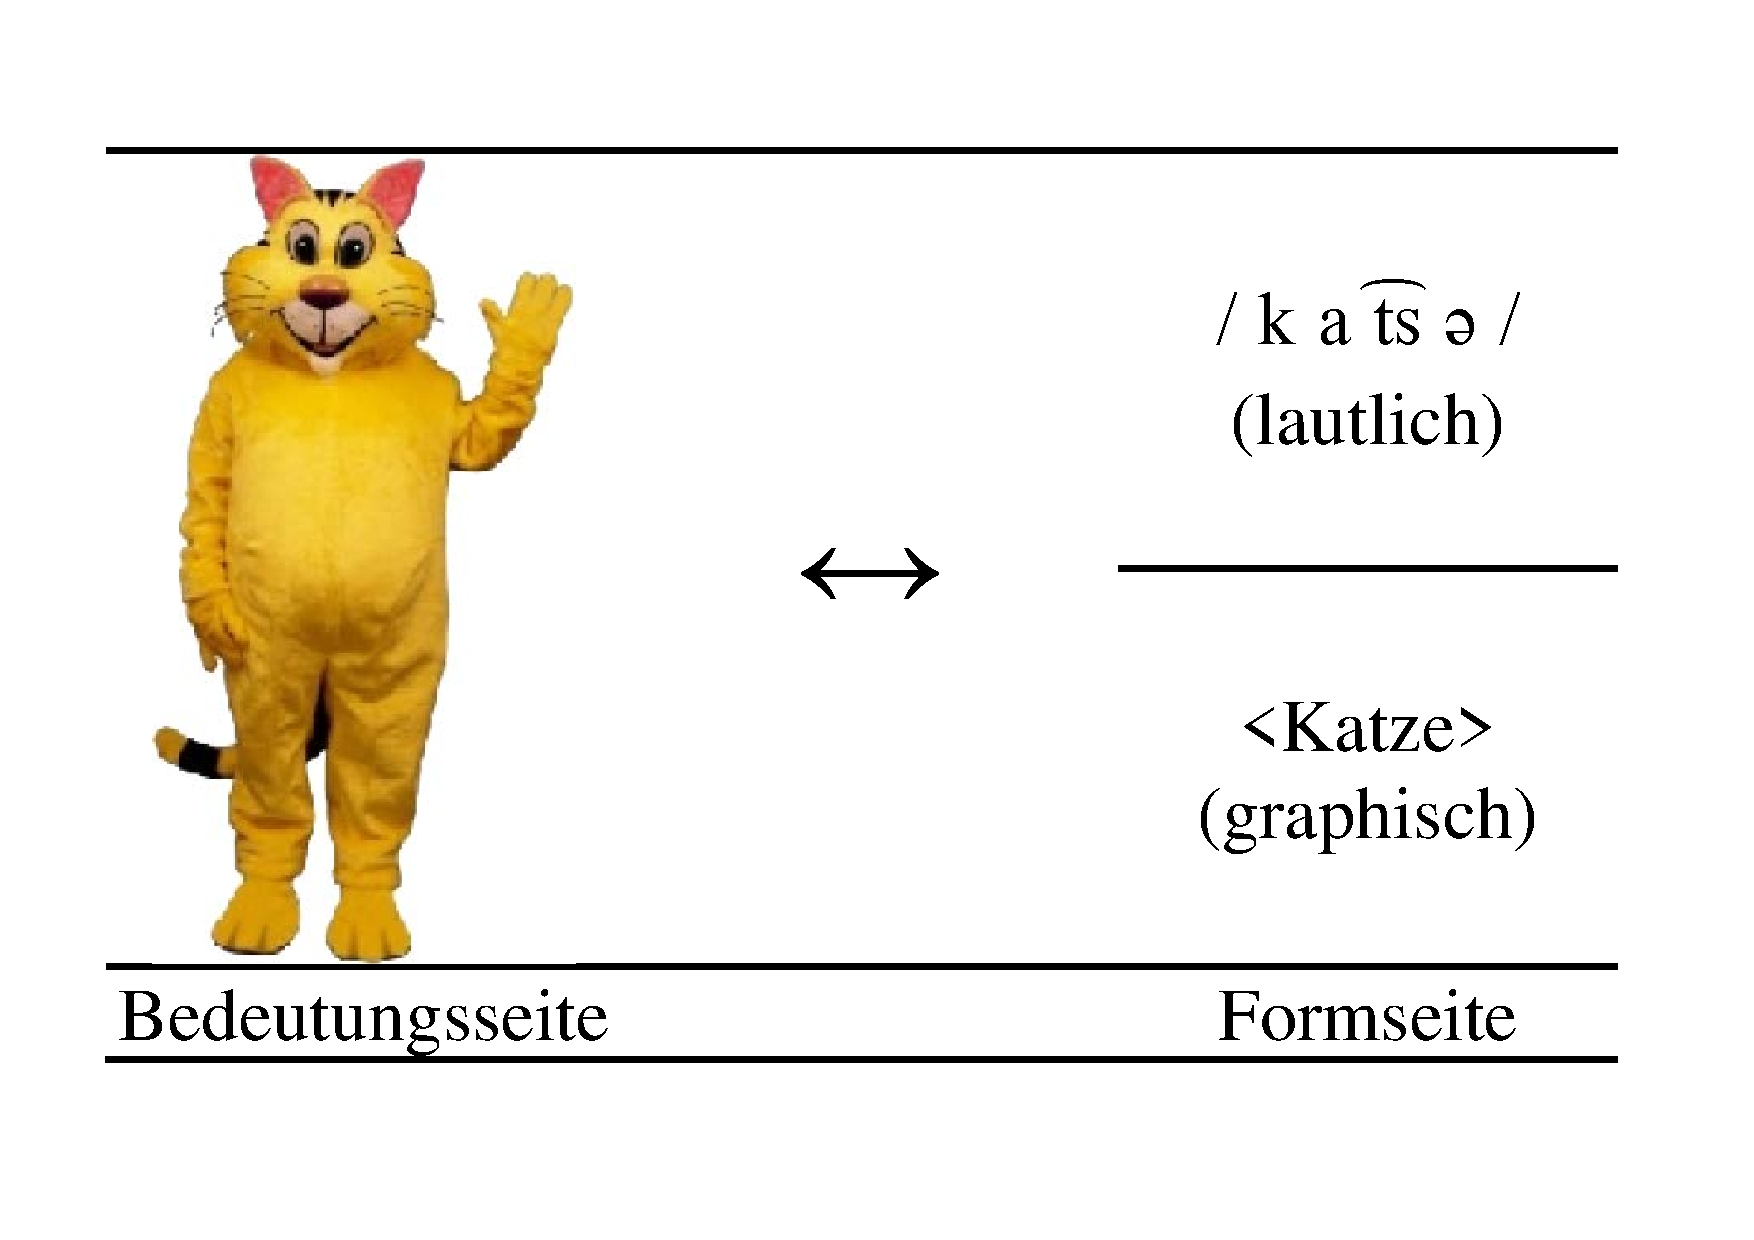
\includegraphics[scale=0.15]{material/01SSZeichenKatze}
%\caption{Beziehung zwischen Funktions-/Bedeutungs- und Formseite}
%\label{Zeichen1}
%\end{figure}

\end{frame}			


%%%%%%%%%%%%%%%%%%%%%%%%%%%%%%%%%%%
%Alternative zur Gelben Katze:

\begin{frame}
\frametitle{Sprachliche Zeichen: Form-Bedeutungs-Paare}
\begin{table}

\centering

\scalebox{1.7}{
\begin{tabular}{c|c}
\multirow{5}*{
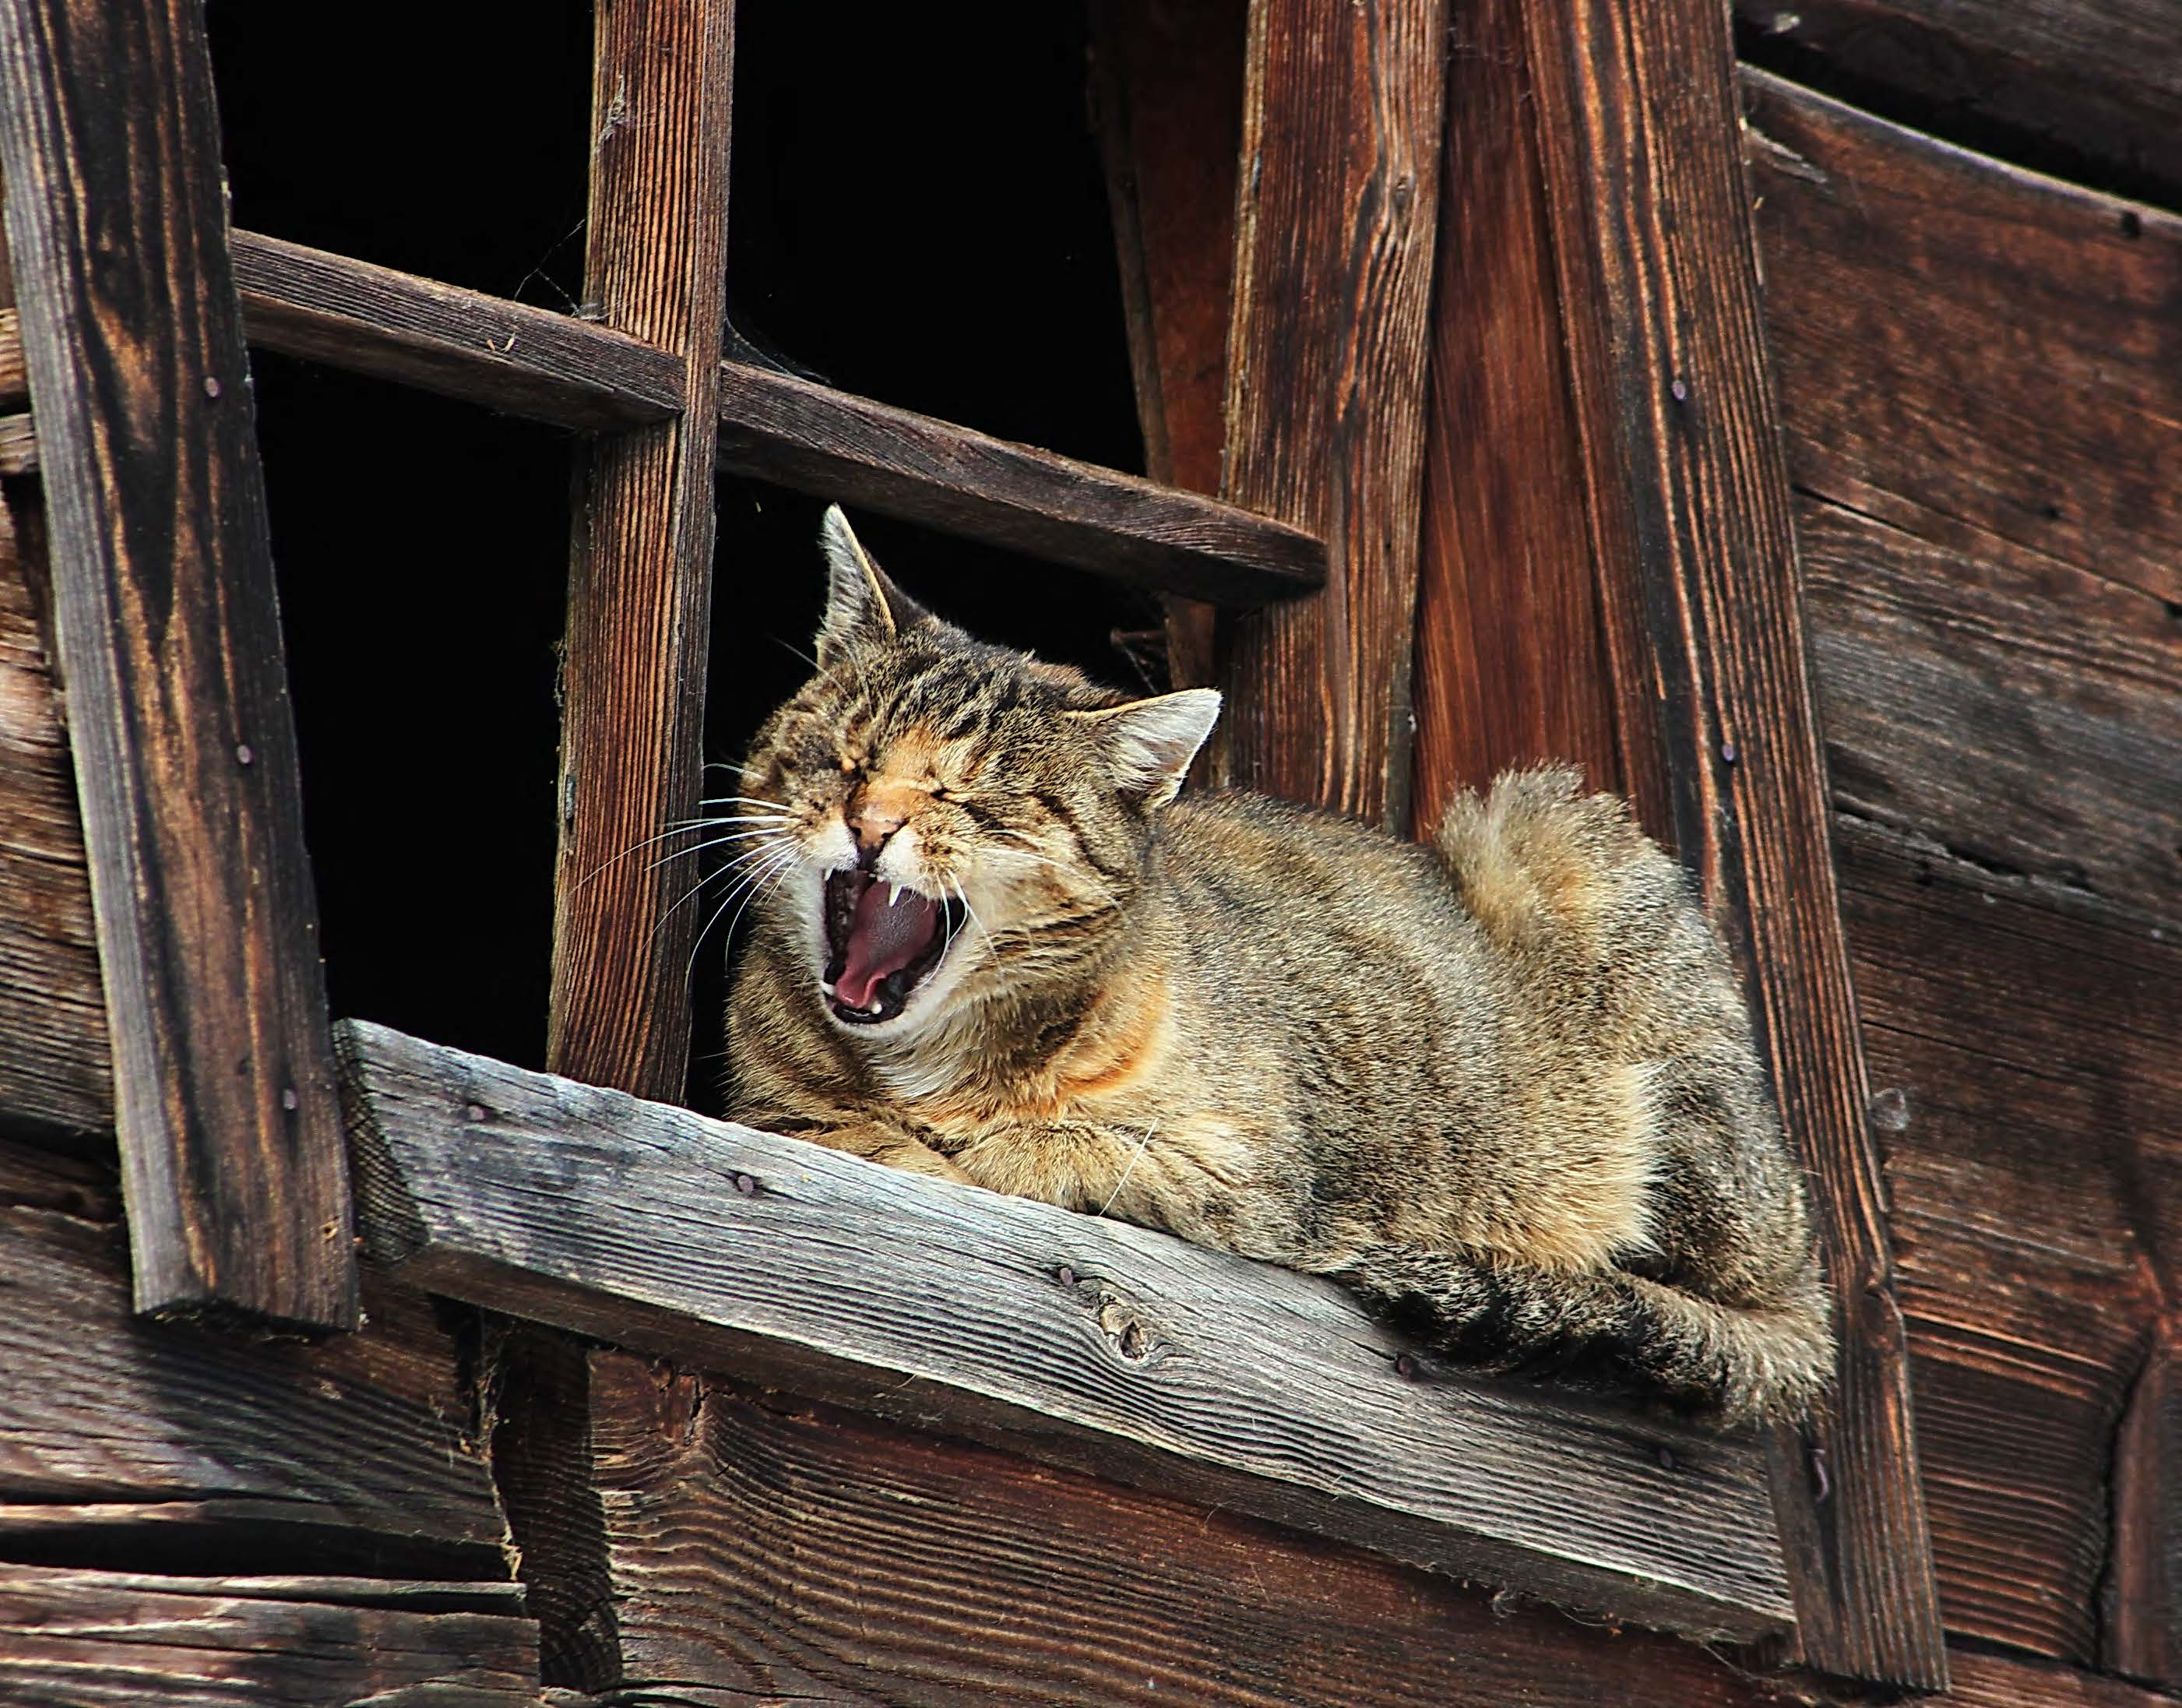
\includegraphics[scale=.024]{material/Hauskatze-an-einem-Scheunenfenster-in-Grossarl}
}&
{\footnotesize /\textipa{ka\t{ts}@}/}\\
&{\tiny (lautlich)}\\
%\cline{2-2}
\\
& {\footnotesize $\langle$Katze$\rangle$} \\
& {\tiny (graphisch)} \\
\hline
{\scriptsize \textbf{Bedeutungsseite}} & {\scriptsize \textbf{Formseite}}\\
\end{tabular}
}
\end{table}

\hfill vgl.\ \citet{Saussure16x}

\end{frame}


%%%%%%%%%%%%%%%%%%%%%%%%%%%%%%%%%%%
\begin{frame}
\frametitle{Zeichensysteme in der Tierkommunikation}

\begin{itemize}
	\item<1-> Tiere verwenden auch Zeichensysteme zur Kommunikation.
\end{itemize}			
			
%\begin{figure}[H]
%\centering

%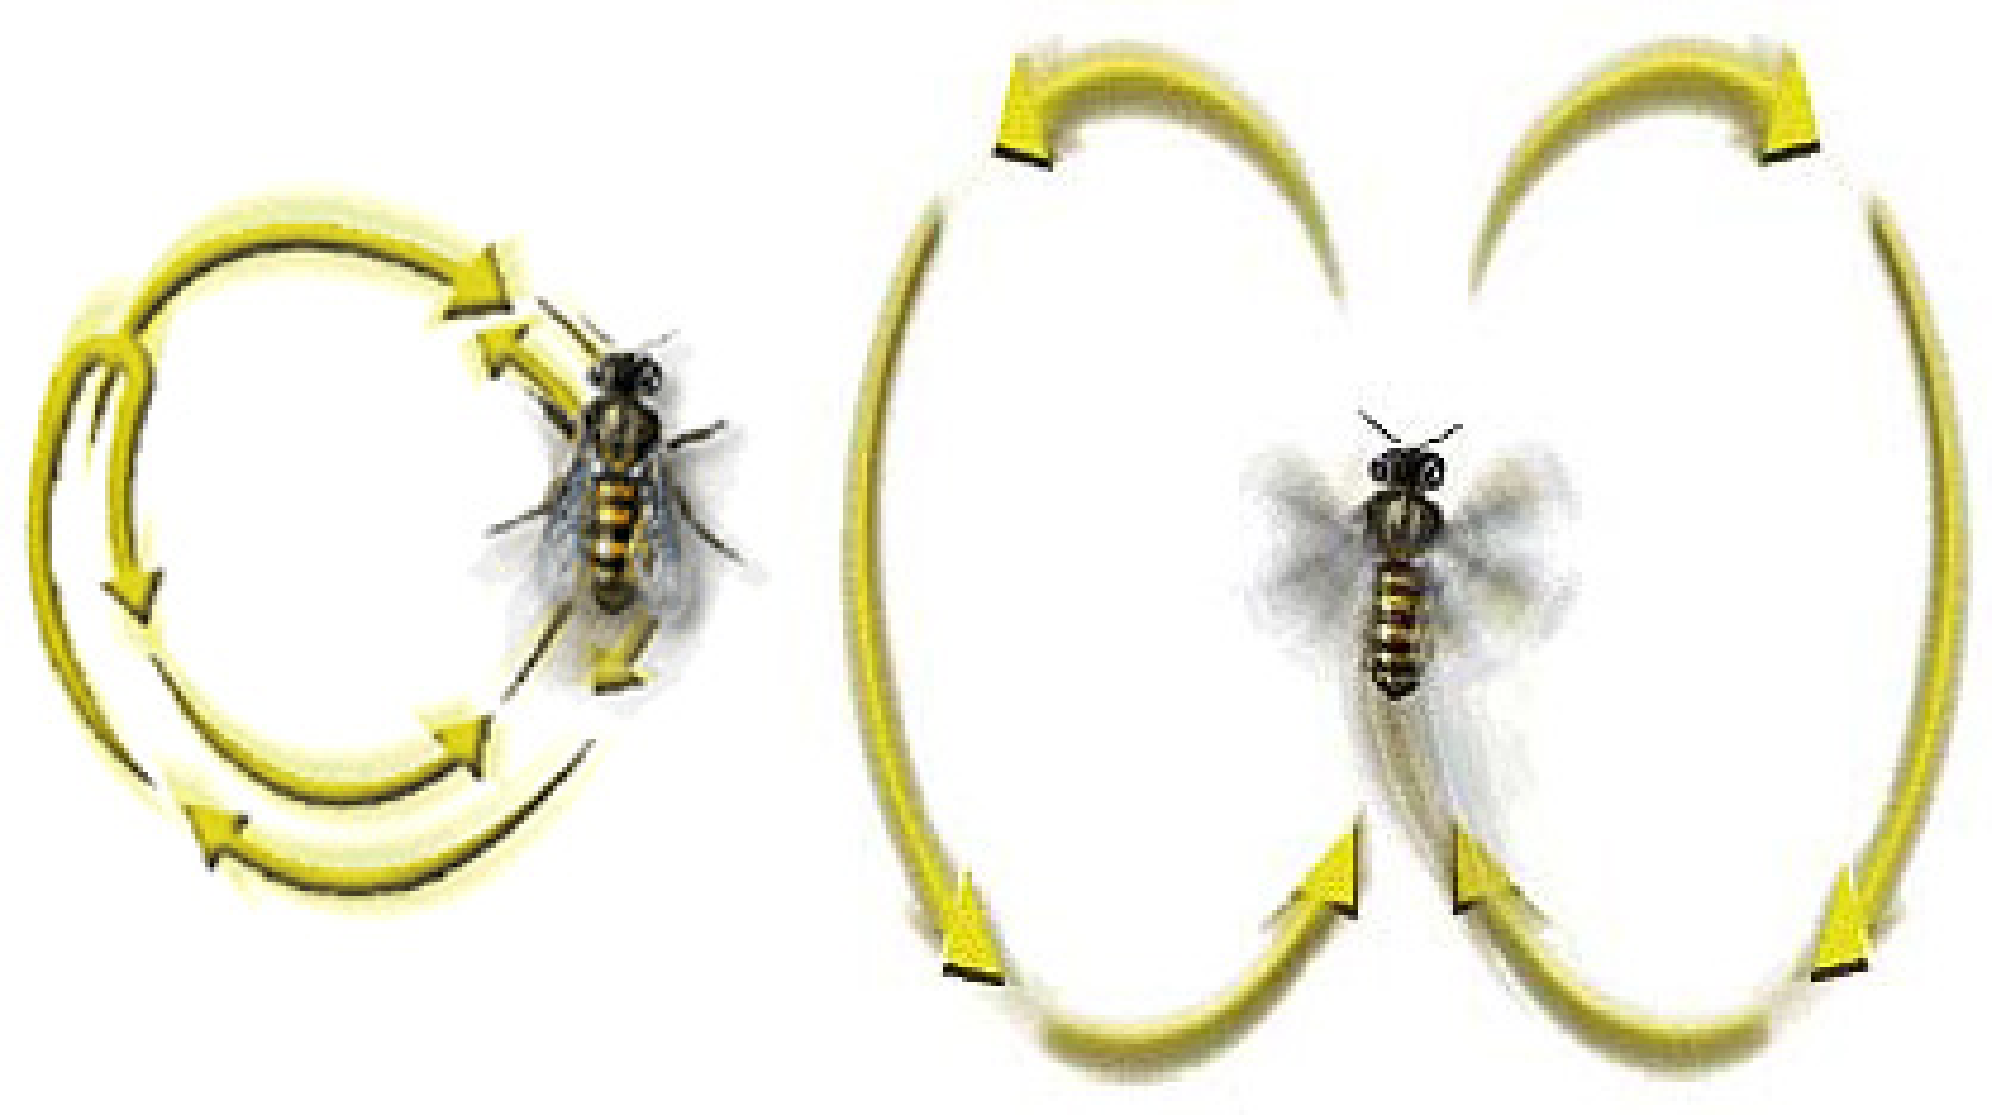
\includegraphics[scale=0.15]{material/01SSBienentanz}
%\caption{\gqq{Rundtanz} und \gqq{Schwänzeltanz} der Bienen}
%\label{Zeichen2}
%\end{figure}



\begin{itemize}
	\item<2-> Mit diesem Zeichensystem teilen Bienen die \textbf{Richtung} und \textbf{Entfernung} der nächsten Nahrungsquelle mit. 
	\item<2-> \textbf{Rundtanz:} Trachtgebiet in der Nähe (weniger als 25\,m)
	\item<2-> \textbf{Schwänzeltanz:} Trachtgebiet bis zu 10\,km weit entfernt, weitere Bewegungen zeigen die Richtung an.

\begin{figure}[H]
\centering
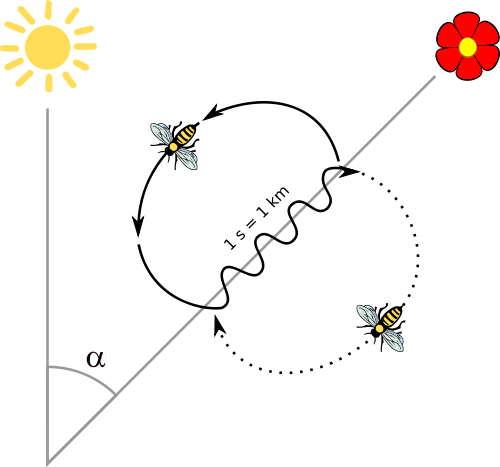
\includegraphics[scale=0.14]{material/Bee-dance}
%\caption{https://commons.wikimedia.org/wiki/File:Bee\_dance.png?uselang=de; GNU-Lizenz; Autor:Audriusa; Bee\_dance/Schwänzeltanz}
\label{Zeichen2}
\end{figure}

\end{itemize}		
		
\end{frame}			


%%%%%%%%%%%%%%%%%%%%%%%%%%%%%%%%%%%
\begin{frame}
\frametitle{Schwänzeltanz}

More than Honey. (R: Markus Imhoof, 2012), 13min 50sec.
%Quelle?

\end{frame}


%%%%%%%%%%%%%%%%%%%%%%%%%%%%%%%%%%%
%%%%%%%%%%%%%%%%%%%%%%%%%%%%%%%%%%%
\subsection{Merkmale natürlicher Sprachen}

%% MyP: Contents
\iftoggle{sectoc}{
	\frame{
		%\begin{multicols}{2}
		\frametitle{~}
		\tableofcontents[currentsubsection, subsubsectionstyle=hide]
		%\end{multicols}
	}
}

%% StM: Contents
\iftoggle{gliederung}{
	
	\outline{
		\begin{itemize}
			
			\item Ziel des Kurses
			\item Sprache und natürliche Sprache
			\item Zeichensysteme
			\item \blaubf{Merkmale natürlicher Sprachen}
			%% Bidirektionalität
			%% Situationelle Ungebundenheit
			%% Rückkopplung
			%% Diskretheit
			%% Produktivität
			%% Arbitrarität
			%% Fazit
			
		\end{itemize}
	}
}
%%%%%%%%%%%%%%%%%%%%%%%%%%%%%%%%%%%
	
\begin{frame}{Merkmale natürlicher Sprachen}

\begin{itemize}
	\item Die menschliche (natürliche) Sprache unterscheidet sich jedoch von anderen Zeichensystemen, wie der \gqq{Bienensprache} oder den Verkehrszeichen, \textbf{nicht in einem einzelnen Merkmal}, sondern \textbf{in einem Bündel von Merkmalen}, welche alle zusammen vorhanden sein müssen (vgl. \citealp{Hockett60a}).
\end{itemize}

\end{frame}


%%%%%%%%%%%%%%%%%%%%%%%%%%%%%%%%%%%
%%%%%%%%%%%%%%%%%%%%%%%%%%%%%%%%%%%
\subsubsection{Bidirektionalität}
%%% MyP: Contents
%\iftoggle{sectoc}{
%	\frame{
%		%\begin{multicols}{2}
%		\frametitle{~}
%		\tableofcontents[currentsubsubsection]
%		%\end{multicols}
%	}
%}
%%%%%%%%%%%%%%%%%%%%%%%%%%%%%%%%%%%

\begin{frame}{Bidirektionalität:}

	\begin{itemize}
		\item[]
		\item<1-> Mensch ist \textbf{sowohl Sender als auch Empfänger} eines Sprachsignals.
		\item[]
		\item<2-> Bei einigen Singvögeln ist das anders:
		
		\begin{itemize}
			\item[]
			\item[$\rightarrow$]<2-> Männchen singen zur Reviermarkierung oder um
                          Weibchen anzulocken.\\
                         Weibchen können oft nicht oder nur wenig singen.\\
                         Sie verstehen den Gesang der Männchen, können ihn aber selbst nicht produzieren.
		\end{itemize}
			
	\end{itemize}

\end{frame}


%%%%%%%%%%%%%%%%%%%%%%%%%%%%%%%%%%%
%%%%%%%%%%%%%%%%%%%%%%%%%%%%%%%%%%%
\subsubsection{Situationelle Ungebundenheit}
%%% MyP: Contents
%\iftoggle{sectoc}{
%	\frame{
%		%\begin{multicols}{2}
%		\frametitle{~}
%		\tableofcontents[currentsubsubsection]
%		%\end{multicols}
%	}
%}
%%%%%%%%%%%%%%%%%%%%%%%%%%%%%%%%%%%

\begin{frame}{Situationelle Ungebundenheit:}
	
	\begin{itemize}
		\item[]
		\item<1-> Menschen sind in der Lage auch über Dinge zu kommunizieren,\\
                          die \textbf{nicht hier und jetzt} stattfinden.
		
		\begin{itemize}
			\item[$\rightarrow$]<2-> Wir können über das leckere gestrige Essen in der Mensa und über unsere Freude auf das morgige Mensafestmahl reden.
		\end{itemize}
		\item<3-> Der Tanz der Bienen ist in diesem Fall der menschlichen Kommunikation ähnlich.
		\item<3-> Einige Primaten sind jedoch nur in der Lage über das Hier und Jetzt zu kommunizieren.
	\end{itemize}
		
\end{frame}


%%%%%%%%%%%%%%%%%%%%%%%%%%%%%%%%%%%
%%%%%%%%%%%%%%%%%%%%%%%%%%%%%%%%%%%
\subsubsection{Rückkopplung}
%%% MyP: Contents
%\iftoggle{sectoc}{
%	\frame{
%		%\begin{multicols}{2}
%		\frametitle{~}
%		\tableofcontents[currentsubsubsection]
%		%\end{multicols}
%	}
%}
%%%%%%%%%%%%%%%%%%%%%%%%%%%%%%%%%%%

\begin{frame}{Rückkopplung}
	
	\begin{itemize}
		\item<1-> Menschen können ihre \textbf{eigenen Sprachsignale} wahrnehmen und darauf reagieren.
		
\ea Ich habe heute \ldots ääähhhh GESTERN die Hausaufgaben abgegeben.
\z

\begin{itemize}
	\item<2->[$\rightarrow$] Der dreistachlige Stichling kann z.\,B. nicht die Färbung seiner Augen und seines Bauches wahrnehmen, die im Balzverhalten eine große Rolle spielt.
\end{itemize}
			\item[]
		\end{itemize}

\end{frame}


%%%%%%%%%%%%%%%%%%%%%%%%%%%%%%%%%%
%%%%%%%%%%%%%%%%%%%%%%%%%%%%%%%%%%
\subsubsection{Diskretheit}
%%% MyP: Contents
%\iftoggle{sectoc}{
%	\frame{
%		%\begin{multicols}{2}
%		\frametitle{~}
%		\tableofcontents[currentsubsubsection]
%		%\end{multicols}
%	}
%}
%%%%%%%%%%%%%%%%%%%%%%%%%%%%%%%%%%%

\begin{frame}{Diskretheit}
			
	\begin{itemize}
		\item Zeichen in natürlichen Sprachen können in kleine, diskrete (\textbf{voneinander unterscheidbare}) \textbf{Einheiten} zerlegt werden.

\pause
				
		\begin{itemize}
			\item[]
			\item[$\rightarrow$] \ab{Alben} und \ab{Alpen} unterscheiden sich nur in der Aussprache eines einzelnen Lautes.
			
			\ea \textipa{[\textglotstop{}al}\alertred{\textipa{b}}\textipa{@n]} vs. \textipa{[\textglotstop{}al}\alertred{\textipa{p}}\textipa{@n]}
			\z 
			
			\item[$\rightarrow$] Der Bienentanz ist eher kontinuierlich als diskret.						
		\end{itemize}
	
	\end{itemize}

\end{frame}


%%%%%%%%%%%%%%%%%%%%%%%%%%%%%%%%%%%
%%%%%%%%%%%%%%%%%%%%%%%%%%%%%%%%%%%
\subsubsection{Produktivität}
%%% MyP: Contents
%\iftoggle{sectoc}{
%	\frame{
%		%\begin{multicols}{2}
%		\frametitle{~}
%		\tableofcontents[currentsubsubsection]
%		%\end{multicols}
%	}
%}
%%%%%%%%%%%%%%%%%%%%%%%%%%%%%%%%%%%

\begin{frame}{Produktivität}
	
	\begin{itemize}
		\item<1-> Eins der wichtigsten Merkmale natürlicher Sprachen!
%		\item[]
		\item<2-> Aus einer \textbf{begrenzten Menge} von \textbf{Lauten} wird eine von
                  Menschen nicht überschaubare Menge von \textbf{Wörtern} und daraus eine unüberschaubare Menge von \textbf{Sätzen} produziert ($\rightarrow$ offenes oder produktives System).
%		\item[]
		\item<2-> Menschen können noch nie gehörte Sätze verstehen und noch nie gesagte Sätze produzieren.

\pause

\ea Meine Freundin hat gestern einen Wasserkocher mit Treueherzen von Kaiser's gekauft.
\ex Meine Freundin von Kaiser's hat gestern Treueherzen mit einem Wasserkocher gekauft.
\z
				
	\item<3-> Der Gibbon (kleiner Menschenaffe) hat ein geschlossenes Rufsystem mit einem kleinen \textbf{endlichen Inventar} an bekannten Lauten. 
	
	\end{itemize}
\end{frame}


%%%%%%%%%%%%%%%%%%%%%%%%%%%%%%%%%%%
%%%%%%%%%%%%%%%%%%%%%%%%%%%%%%%%%%%
\subsubsection{Arbitrarität}
%%% MyP: Contents
%\iftoggle{sectoc}{
%	\frame{
%		%\begin{multicols}{2}
%		\frametitle{~}
%		\tableofcontents[currentsubsubsection]
%		%\end{multicols}
%	}
%}
%%%%%%%%%%%%%%%%%%%%%%%%%%%%%%%%%%%

\begin{frame}{Arbitrarität}

\begin{itemize}
	\item<1-> \textbf{Bezeichnendes} (Signifikant, frz.\ signifiant) ist nicht durch \textbf{Bezeichnetes} (Signifikat, frz. signifié) bestimmt.
	\item[]
	\item<2-> Verschiedene Sprachen haben unterschiedliche Namen (Bezeichnendes) für das gleiche Objekt (Bezeichnetes):

\pause

\ea dt. \ab{Stift}, engl. \ab{pen}, sp. \ab{bolígrafo}, frz. \ab{crayon}, \ldots
\z

\pause 

	\item Benennung ist \textbf{konventionell}, \dash in der Sprachgemeinschaft festgelegt.

	\begin{itemize}
		\item[$\rightarrow$] Der Tanz der Bienen ist nicht arbiträr, sondern motiviert.
	\end{itemize}

\pause
		
	\item Es gibt in natürlichen Sprachen \textbf{auch motivierte} Zeichen:

\ea Deutsch und Dänisch \textipa{[va\textupsilon{} va\textupsilon{}]}, Griechisch \textipa{[gav gav]}, Russisch \textipa{[gaf gaf]}, Spanisch \textipa{[g\textupsilon{}au g\textupsilon{}au]}, Französisch \textipa{[g\textupsilon{}af g\textupsilon{}af]}, Englisch \textipa{[w\textopeno{}f w\textopeno{}f]}, Litauisch \textipa{[a\textupsilon{} a\textupsilon{}]}, Koreanisch \textipa{[m\textopeno{}N m\textopeno{}N]}
\z

\end{itemize}

\end{frame}


%%%%%%%%%%%%%%%%%%%%%%%%%%%%%%%%%%%
%%%%%%%%%%%%%%%%%%%%%%%%%%%%%%%%%%%
\subsubsection{Fazit}
%%% MyP: Contents
%\iftoggle{sectoc}{
%	\frame{
%		%\begin{multicols}{2}
%		\frametitle{~}
%		\tableofcontents[currentsubsubsection]
%		%\end{multicols}
%	}
%}
%%%%%%%%%%%%%%%%%%%%%%%%%%%%%%%%%%%
\begin{frame}{Fazit}
		
	\begin{block}{Natürliche Sprache}
			Insgesamt bildet die natürliche Sprache also ein \textbf{produktives}, \textbf{bidirektionales}, \textbf{arbiträres} und \textbf{diskretes} Symbolsystem (vgl. \citealp{Luedeling2009a}).
	\end{block}

\end{frame}	

%%%%%%%%%%%%%%%%%%%%%%%%%%%%%%%%%%%
%\begin{frame}{Übung}
%	Wie unterscheiden sich Computersprachen von natürlichen Sprachen? Diskutieren Sie dies anhand der eingeführten Kriterien.
%\end{frame}
%
%%%%%%%%%%%%%%%%%%%%%%%%%%%%%%%%%%%
%\iftoggle{ue-loesung}{
%	
%\begin{frame}{Übung -- Lösung}
%Wie unterscheiden sich Computersprachen von natürlichen Sprachen? Diskutieren Sie dies anhand der eingeführten Kriterien.
%
%{\red
%	
%\begin{itemize}
%\item Produktivität: ja, 
%\item Bidirektionalität:
%\item Arbitrarität: 
%\item Diskretheit: 
%\end{itemize}
%
%}
%
%\end{frame}
%
%}

%%%%%%%%%%%%%%%%%%%%%%%%%%%%%%%%%%%
%%%%%%%%%%%%%%%%%%%%%%%%%%%%%%%%%%%
\subsection*{Quellen}
%%%%%%%%%%%%%%%%%%%%%%%%%%%%%%%%%%%

\begin{frame}{Quellen}
	
	
	\begin{itemize}
		\item ABBILDUNG -- \gqq{Hauskatze} (Zugriff: 02.08.2019): \url{https://commons.wikimedia.org/wiki/File:Hauskatze\_an\_einem\_Scheunenfenster\_in\_Grossarl.JPG}
		%\medskip
		\item ABBILDUNG -- \gqq{Bienentanz} (Zugriff: 02.08.2019):
		\url{https://commons.wikimedia.org/wiki/File:Bee\_dance.png?uselang=de}
                \item VIDEO -- 	\textit{More than Honey}. Regie: Markus Imhoof. Drehbuch: Markus Imhoof, Kerstin Hoppenhaus. Schweiz/Deutschland/Österreich 2012. Fassung: DVD, 95 Min.
	\end{itemize}	
	
\end{frame}


%% %%%%%%%%%%%%%%%%%%%%%%%%%%%%%%%%%%%
%% %%%%%%%%%%%%%%%%%%%%%%%%%%%%%%%%%%%
%% \subsection*{Elektronische Quellen}
%% %%%%%%%%%%%%%%%%%%%%%%%%%%%%%%%%%%%

%% \begin{frame}{Elektronische Quellen}
	
	
	
%% 	\begin{itemize}
%% 		\item VIDEO -- 	\textit{More than Honey}. Regie: Markus Imhoof. Drehbuch: Markus Imhoof, Kerstin Hoppenhaus. Schweiz/Deutschland/Österreich 2012. Fassung: DVD, 95 Min.
%% 	\end{itemize}
	
%% \end{frame}


%%%%%%%%%%%%%%%%%%%%%%%%%%%%%%%%%%%%%%%%%%%%%%%%
%% Compile the master file!
%% 		Slides: Antonio Machicao y Priemer
%% 		Course: GK Linguistik
%%%%%%%%%%%%%%%%%%%%%%%%%%%%%%%%%%%%%%%%%%%%%%%%


%%%%%%%%%%%%%%%%%%%%%%%%%%%%%%%%%%%%%%%%%%%%%%%%%%%%
%%%             Metadata                         
%%%%%%%%%%%%%%%%%%%%%%%%%%%%%%%%%%%%%%%%%%%%%%%%%%%%      

\title{Grundkurs Linguistik}

\subtitle{Sprache \& Sprachwissenschaft II}

\author[A. Machicao y Priemer]{
	{\small Antonio Machicao y Priemer}
	\\
	{\footnotesize \url{http://www.linguistik.hu-berlin.de/staff/amyp}}
	%	\\
	%	\href{mailto:mapriema@hu-berlin.de}{mapriema@hu-berlin.de}}
}

\institute{Institut für deutsche Sprache und Linguistik}

\date{ }

%\publishers{\textbf{6. linguistischer Methodenworkshop \\ Humboldt-Universität zu Berlin}}

%\hyphenation{nobreak}


%%%%%%%%%%%%%%%%%%%%%%%%%%%%%%%%%%%%%%%%%%%%%%%%%%%%
%%%             Preamble's End                   
%%%%%%%%%%%%%%%%%%%%%%%%%%%%%%%%%%%%%%%%%%%%%%%%%%%%       


%%%%%%%%%%%%%%%%%%%%%%%%%      
\huberlintitlepage[22pt]

\iftoggle{toc}{
\frame{
\begin{multicols}{2}
	\frametitle{Inhaltsverzeichnis}
	\tableofcontents
	%[pausesections]
\end{multicols}
	}
	}

%%%%%%%%%%%%%%%%%%%%%%%%%%%%%%%%%%
%%%%%%%%%%%%%%%%%%%%%%%%%%%%%%%%%%
%%%%%LITERATURE:

%% Allgemein
\nocite{Glueck&Roedel16a}
\nocite{Schierholz&Co18}
\nocite{Luedeling2009a}
\nocite{Meibauer&Co07a} 
\nocite{Repp&Co15a} 

%% Sprache & Sprachwissenschaft
\nocite{Fries16c} %Adäquatheit
\nocite{Fries16a} %Grammatikalität
\nocite{Fries&MyP16c} %GG
\nocite{Fries&MyP16b} %Akzeptabilität
\nocite{Fries&MyP16d} %Kompetenz vs. Performanz
\nocite{MuellerGT-Eng2} %Grammatical Theory (2nd Ed.)


%%%%%%%%%%%%%%%%%%%%%%%%%%%%%%%%%%%
%%%%%%%%%%%%%%%%%%%%%%%%%%%%%%%%%%%
\section{Sprache \& Sprachwissenschaft II}

%%%%%%%%%%%%%%%%%%%%%%%%%%%%%%%%%%%
	
	
%%%%%%%%%%%%%%%%%%%%%%%%%%%%%%%%%%%
%%%%%%%%%%%%%%%%%%%%%%%%%%%%%%%%%%%
\subsection{Grammatik}
%% MyP: Contents
\iftoggle{sectoc}{
\frame{
%\begin{multicols}{2}
\frametitle{~}
	\tableofcontents[currentsubsection, subsubsectionstyle=hide]
%\end{multicols}
}
}

%% StM: Contents
\iftoggle{gliederung}{
	
	\outline{
		\begin{itemize}
			
			\item \blaubf{Grammatik}
			\item Grammatikbegriff
			\item Modularität der Grammatik
			%% Lexikon
			%% Phonologische Komponente
			%% Morphologische Komponente
			%% Syntaktische Komponente
			%% Semantische Komponente
			%% Architektur des Sprachsystems
			\item Linguistische Teildisziplinen
			\item Linguistik als Geistes- und/oder Naturwissenschaft
			\item Sprachwissenschaft \vs Linguistik
			
		\end{itemize}
	}
}
%%%%%%%%%%%%%%%%%%%%%%%%%%%%%%%%%%%
	
\begin{frame}{Grammatik}
	\begin{itemize}
		\item Komplexität des Sprachsystems (Einheiten + Regeln) ist den Sprechern meist \textbf{nicht bewusst}.
		\item[]
		\item Die Linguistik interessiert sich für das unbewusste, internalisierte System, d.h.\ für die sprachliche \textbf{Kompetenz} der Sprecher.
		\item[]
		\item Diese Kompetenz bildet die Grammatik einer Sprache.
	\end{itemize}
	
	\begin{block}<2->{Grammatik}
		System, das Laute/""Lautkombinationen und Bedeutungen \textbf{regelhaft einander zuordnet} und das gesamte Regelsystem einer Sprache umfasst.
	\end{block}	
\end{frame}


%%%%%%%%%%%%%%%%%%%%%%%%%%%%%%%%%%%
%%%%%%%%%%%%%%%%%%%%%%%%%%%%%%%%%%%
\subsection{Grammatikbegriff}

%% MyP: Contents
\iftoggle{sectoc}{
\frame{
%\begin{multicols}{2}
\frametitle{~}
	\tableofcontents[currentsubsection, subsubsectionstyle=hide]
%\end{multicols}
}
}

%% StM: Contents
\iftoggle{gliederung}{
	
	\outline{
		\begin{itemize}
			
			\item Grammatik
			\item \blaubf{Grammatikbegriff}
			\item Modularität der Grammatik
			%% Lexikon
			%% Phonologische Komponente
			%% Morphologische Komponente
			%% Syntaktische Komponente
			%% Semantische Komponente
			%% Architektur des Sprachsystems
			\item Linguistische Teildisziplinen
			\item Linguistik als Geistes- und/oder Naturwissenschaft
			\item Sprachwissenschaft \vs Linguistik
			
		\end{itemize}
	}
}
%%%%%%%%%%%%%%%%%%%%%%%%%%%%%%%%%%%

\begin{frame}{Grammatikbegriff}

\begin{itemize}
	\item<1-> Grammatik im engeren Sinne als \textbf{Lehre} von \textbf{morphologischen} und \textbf{syntaktischen} Regularitäten einer Sprache. Unter dieser Auffassung bleiben die Phonologie und die Semantik als Teilbereiche der Sprachwissenschaft ausgeklammert (\textbf{traditionelle Definition}).
	\item[]
	\item<2-> Grammatik als \textbf{präskriptive/normative} Grammatik, die Vorgaben für die \gqq{korrekte} Sprachverwendung einer einzelnen Sprache (\gqq{gutes Deutsch}) macht (\zB \citealp{DudenGramm09d}).
	\item[]
	\item<3-> Grammatik als \textbf{deskriptive} Grammatik, die eine wertungsfreie Beschreibung einer einzelnen Sprache gibt (\zB \citealp{Eisenberg00a}, auch \gqq{Problemgrammatik} genannt).
\end{itemize}

\end{frame}

%%%%%%%%%%%%%%%%%%%%%%%%%%%%%%%%%%%%%%%

\begin{frame}

	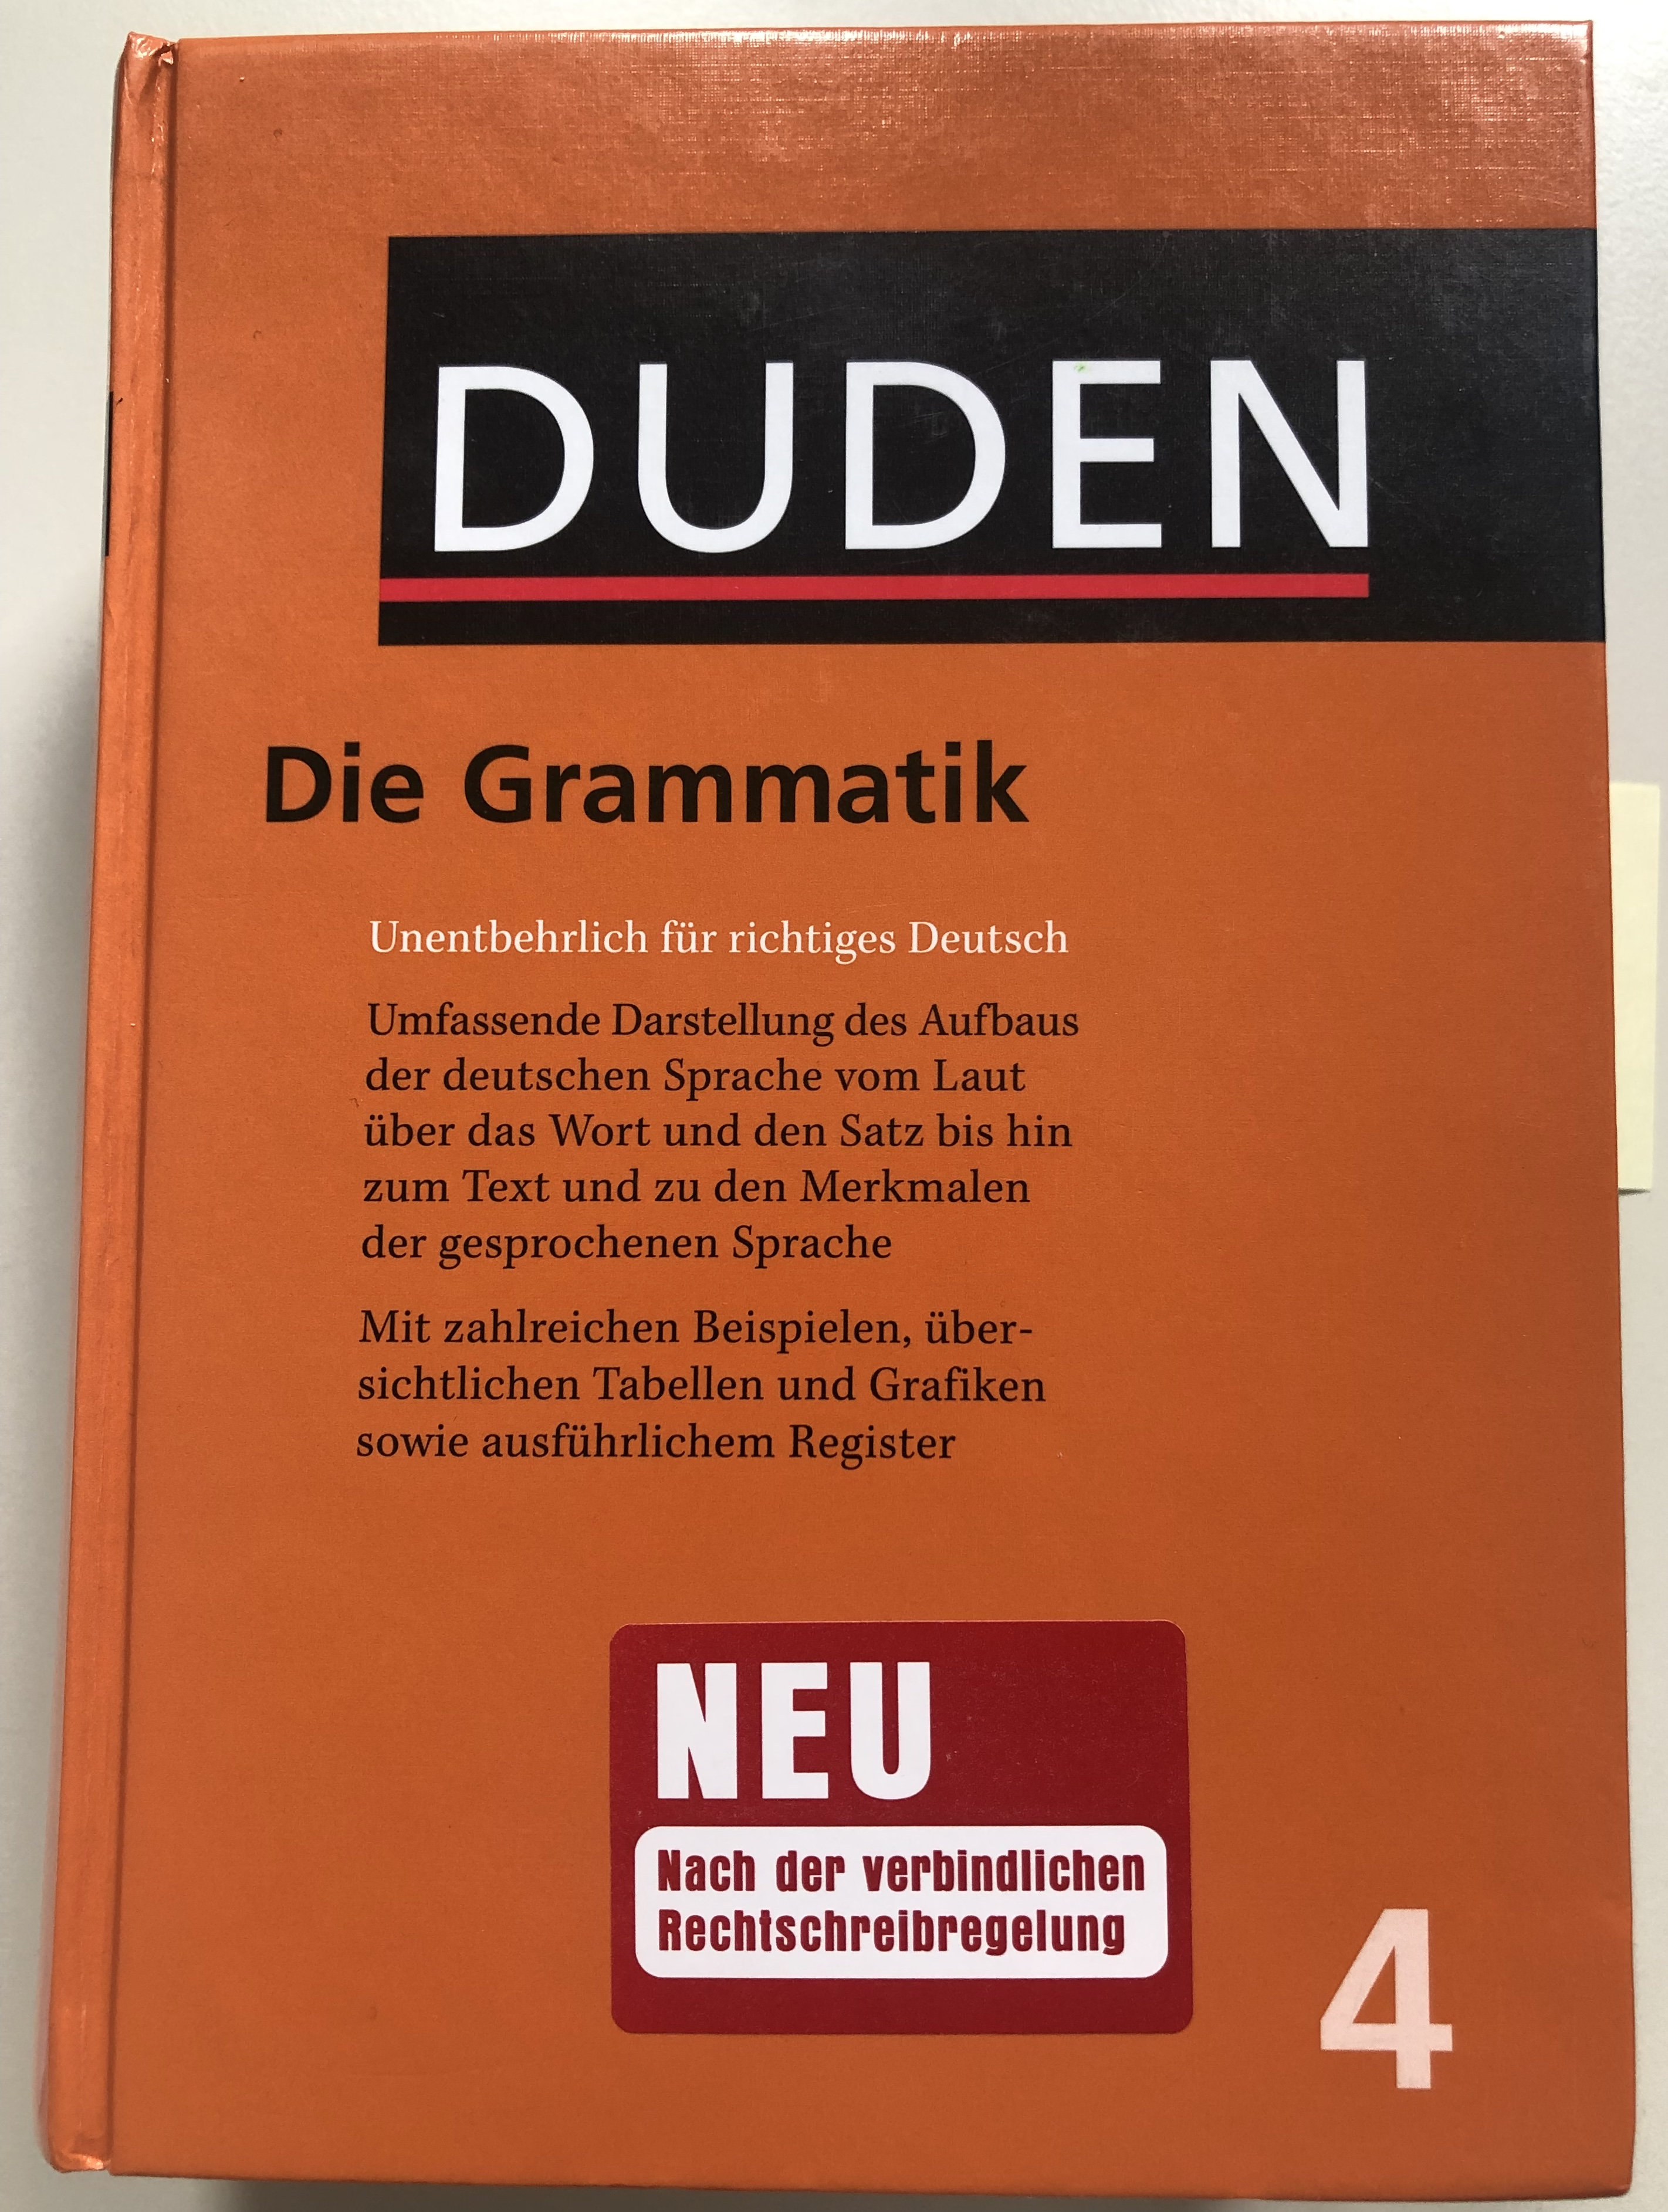
\includegraphics[width=.45\textwidth]{material/DudenRichtigesDeutsch}

\end{frame}


%%%%%%%%%%%%%%%%%%%%%%%%%%%%%%%%%%%
\begin{frame}

\begin{itemize}
	\item<1-> Grammatik als \textbf{Lehrbuch} oder \textbf{Nachschlagewerk}
	\item[]
	\item<2-> Grammatik für den Fremdsprachenunterricht (\zB \citealp{Helbig&Buscha05a})
	\item[]
	\item<3-> Grammatik als \textbf{Sprachtheorie} \citep[vgl.][]{MuellerGT-Eng2}, \zB Generative Grammatik (GG) (vgl. \citealp{Philippi&Tewes10a}) oder Dependenzgrammatik (vgl. \citealp{Agel00a})
	\item[]
	\item<4-> In diesem Seminar verstehen wir \textbf{Grammatik} als:

	\begin{itemize}
		\item<4-> \textbf{System}, das Laute und Bedeutungen regelhaft einander zuordnet und das gesamte Regelsystem einer Sprache umfasst.
		\item<4-> Wir befassen uns mit Grammatik mit einer \textbf{deskriptiven} Methodik
                  (d.\,h. nicht präskriptiv) und verwenden dafür (bzw.\ bilden dadurch)
                  \textbf{Grammatiktheorien} (z.\,B. GG).
	\end{itemize}

\end{itemize}

\end{frame}


%%%%%%%%%%%%%%%%%%%%%%%%%%%%%%%%%%%
%%%%%%%%%%%%%%%%%%%%%%%%%%%%%%%%%%%
\subsection{Modularität der Grammatik}

%% MyP: Contents
\iftoggle{sectoc}{
\frame{
%\begin{multicols}{2}
\frametitle{~}
	\tableofcontents[currentsubsection, subsubsectionstyle=hide]
%\end{multicols}
}
}

%% StM: Contents
\iftoggle{gliederung}{
	
	\outline{
		\begin{itemize}
			
			\item Grammatik
			\item Grammatikbegriff
			\item \blaubf{Modularität der Grammatik}
			%% Lexikon
			%% Phonologische Komponente
			%% Morphologische Komponente
			%% Syntaktische Komponente
			%% Semantische Komponente
			%% Architektur des Sprachsystems
			\item Linguistische Teildisziplinen
			\item Linguistik als Geistes- und/oder Naturwissenschaft
			\item Sprachwissenschaft \vs Linguistik
			
		\end{itemize}
	}
}
%%%%%%%%%%%%%%%%%%%%%%%%%%%%%%%%%%%

\begin{frame}{Modularität der Grammatik}
	
\begin{itemize}
	\item hauptsächlich in der Generativen Grammatik angenommen\\
              (in anderen Grammatiktheorietraditionen umstritten)
	\medskip
	\item Sprachvermögen $\rightarrow$ modular organisiert
	\medskip
	\item<2-> Grammatik (oder Sprache) ist ein \textbf{Modul} im \textbf{menschlichen kognitiven System}.
	\item<2-> Dieses (Sprach)modul besteht zugleich aus \textbf{miteinander interagierenden Teilmodulen} (auch sprachlichen Teilmodulen, grammatischen Ebenen oder sprachlichen Komponenten).
	\medskip
	\item<3-> Wie \textbf{selbstständig} diese Module sind, ist umstritten.
	\medskip
	\item<3-> Die \textbf{Evidenz} für eine Modularisierung findet die GG in der Aphasie-, Versprecher- und Spracherwerbsforschung.  
\end{itemize}

\end{frame}


%%%%%%%%%%%%%%%%%%%%%%%%%%%%%%%%%%%
\begin{frame}
\frametitle{Module}
\begin{itemize}
	\item Folgende Module werden angenommen (vgl. \citealp{Abramowski2016}):
		
	\begin{itemize}
%		\item[]
		\item Lexikon
%		\item[]
		\item Phonologische Komponente
%		\item[]
		\item Morphologische Komponente
%		\item[]
		\item Syntaktische Komponente
%		\item[]
		\item Semantische Komponente
%		\item[]
	\end{itemize}
		
	\item<2-> Jedes sprachliche Modul besteht zugleich aus:
	
	\begin{enumerate}
		\item<2-> einem Inventar von komponentenspezifisch kategorisierten \textbf{Minimaleinheiten}\\
                         (\zB Morphem in der Morphologie) und
		\item<2-> einer Menge von komponentenspezifischen \textbf{Regeln zur Kombination} dieser Minimaleinheiten zu wohlgeformten komplexen Einheiten. 
	\end{enumerate}		  
		
\end{itemize}

\end{frame}


%%%%%%%%%%%%%%%%%%%%%%%%%%%%%%%%%%%
%%%%%%%%%%%%%%%%%%%%%%%%%%%%%%%%%%%
\subsubsection{Lexikon}
%%% MyP: Contents
%\iftoggle{sectoc}{
%	\frame{
%		%\begin{multicols}{2}
%		\frametitle{~}
%		\tableofcontents[currentsubsubsection]
%		%\end{multicols}
%	}
%}
%%%%%%%%%%%%%%%%%%%%%%%%%%%%%%%%%%%

\begin{frame}{Lexikon}
	
	\begin{itemize}
		\item \textbf{Repräsentation von Wörtern} und Wortteilen einer Sprache mit der \textbf{Information} über deren:

		\begin{enumerate}
			\item[]
			\item Aussprache (phonologische Information)
			\item[]
			\item interne Struktur (morphologische Information)
			\item[]
			\item syntaktische Kategorie und syntaktisches Kombinationspotential (syntaktische Information)
			\item[]
			\item Bedeutung (semantische Information) 
			\item[]
			\item idiosynkratische Information (nicht ableitbare Information)
		\end{enumerate}		  
			
	\end{itemize}
		
\end{frame}


%%%%%%%%%%%%%%%%%%%%%%%%%%%%%%%%%%%
\begin{frame}{Lexikon}
			
\begin{itemize}
	\item Eintrag für den Verbstamm \emph{geb-} (von \emph{geben}): \ab{\textsc{geb-}}

	\begin{enumerate}
		\item[]
		\item Phonologische Information: \textipa{/ge\textlengthmark{}b/}
		\item[]
		\item Morphologische Information: [\textsubscript{V-Stamm}\ab{geb-}] 
		\item[]
		\item Syntaktische Information (ditransitives Verb):\\
			NP\textsubscript{\alertred{1}\{\textsc{nom}\}}$+$
			NP\textsubscript{\alertred{2}\{\textsc{dat}\}}$+$
			NP\textsubscript{\alertred{3}\{\textsc{akk}\}}$+$
			V
					
		\item[]
		\item Semantische Information (Verb des Besitzwechsels):\\
			NP\textsubscript{\alertred{1}\{\textsc{agens}\}}$+$
			NP\textsubscript{\alertred{2}\{\textsc{goal}\}}$+$
			NP\textsubscript{\alertred{3}\{\textsc{thema}\}}$+$
			V \\
			$\approx$
			\gq{NP\textsubscript{\alertred{1}} macht, dass NP\textsubscript{\alertred{2}} NP\textsubscript{\alertred{3}} erhält.} 
	\end{enumerate}		  


\ea (\dots dass) Luise\MyPdown{\alertred{1}} Jacob\MyPdown{\alertred{2}} das Buch\MyPdown{\alertred{3}} gibt
\z 
\end{itemize}

\end{frame}


%%%%%%%%%%%%%%%%%%%%%%%%%%%%%%%%%%%
%%%%%%%%%%%%%%%%%%%%%%%%%%%%%%%%%%%
\subsubsection{Phonologische Komponente}
%%% MyP: Contents
%\iftoggle{sectoc}{
%	\frame{
%		%\begin{multicols}{2}
%		\frametitle{~}
%		\tableofcontents[currentsubsubsection]
%		%\end{multicols}
%	}
%}
%%%%%%%%%%%%%%%%%%%%%%%%%%%%%%%%%%%

\begin{frame}{Phonologische Komponente}

	\begin{itemize}
		\item Sie beschränkt das \textbf{Lautinventar} einer Sprache.
\medskip
		\item Sie regelt die \textbf{Lautkombinatorik} und \textbf{-veränderung}.
\medskip
		\item Festlegung von \textbf{Wort-} und \textbf{Satzakzent}:
\pause
\bigskip
		\item[\ra] Wieso spricht man \ab{Hund} mit \textipa{[t]} aber \ab{Hunde} mit \textipa{[d]} aus?
\pause
		\item[\ra] Kann ein Wort im Deutschen mit der Lautfolge \textipa{[Ng]} beginnen?
\pause
		\item[\ra] Was ist der Unterschied zwischen \abu{HAUStürgriff} und \abu{HausTÜRgriff}?
	\end{itemize}
	
\end{frame}


%%%%%%%%%%%%%%%%%%%%%%%%%%%%%%%%%%%
%%%%%%%%%%%%%%%%%%%%%%%%%%%%%%%%%%%
\subsubsection{Morphologische Komponente}
%%% MyP: Contents
%\iftoggle{sectoc}{
%	\frame{
%		%\begin{multicols}{2}
%		\frametitle{~}
%		\tableofcontents[currentsubsubsection]
%		%\end{multicols}
%	}
%}
%%%%%%%%%%%%%%%%%%%%%%%%%%%%%%%%%%%

\begin{frame}{Morphologische Komponente}

\begin{itemize}
	\item Sie regelt die \textbf{interne Struktur von Wörtern}.
\medskip
	\item Bildung von neuen Wörtern und Wortformen
\pause
\bigskip
	\item[\ra] Wie hängen \ab{kaufen} und \ab{kaufbar} zusammen?
\pause
	\item[\ra] Was zeigt \ab{-st} bei der Bildung neuer Verbformen an?
\end{itemize}

\end{frame}


%%%%%%%%%%%%%%%%%%%%%%%%%%%%%%%%%%%
\begin{frame}{Morphologische Komponente}

	\ea Warum ist die eine Struktur des Wortes \ab{Bedeutungsableitung} intuitiv nicht korrekt und die andere schon?
	\z
			

\begin{columns}

\column[b]{.4\linewidth}		
\begin{figure}[b]
	
\scriptsize{
		\begin{forest}MyP edges
		[Bedeutungsableitung [Be][deutungsableitung [deut][ungsableitung [ungsableit [ung][sableit [sab [s][ab]][leit]]][ung]]]]
		\end{forest}
}
		
\caption{Ungrammatisch}

\end{figure}

\column[b]{.4\linewidth}
\begin{figure}[b]
	\scriptsize{
		\begin{forest}MyP edges
		[Bedeutungsableitung [Bedeutungs [Bedeutung [Bedeut [Be][deut]][ung]][s]][ableitung [ableit [ab][leit]][ung]]]
		\end{forest}}
			
	\caption{Grammatisch}

\end{figure}

\end{columns}
\end{frame}


%%%%%%%%%%%%%%%%%%%%%%%%%%%%%%%%%%%
%%%%%%%%%%%%%%%%%%%%%%%%%%%%%%%%%%%
\subsubsection{Syntaktische Komponente}
%%% MyP: Contents
%\iftoggle{sectoc}{
%	\frame{
%		%\begin{multicols}{2}
%		\frametitle{~}
%		\tableofcontents[currentsubsubsection]
%		%\end{multicols}
%	}
%}
%%%%%%%%%%%%%%%%%%%%%%%%%%%%%%%%%%%
	
\begin{frame}{Syntaktische Komponente}

\begin{itemize}
	\item Sie regelt die \textbf{Struktur} von \textbf{Phrasen und Sätzen}.
\pause
\bigskip
	\item[\ra] Wieso ist die Phrase (\ref{ex1a}) grammatisch und die Phrase (\ref{ex1b}) nicht?
	\ea
		\ea[ ]{die Königin von Schweden aus Deutschland}\label{ex1a}
		\ex[*]{die Königin aus Deutschland von Schweden}\label{ex1b}
		\z
	\z
\pause
	\item[\ra] Warum ist ein Satz wie (\ref{ex2a}) ungrammatisch (trotz alphabetischer Anordnung der Wörter), während (\ref{ex2b}) grammatisch ist?
	\ea
		\ea[*]{Buch Chomsky das ich kaufen morgen von werde.}\label{ex2a}
		\ex[]{Das Buch von Chomsky werde ich morgen kaufen.}\label{ex2b}
		\z
	\z
\pause	
	\item[\ra] Aus welchem Grund hat der Satz unter (\ref{ex3}) zwei Bedeutungen? 
	\ea
		\ea Maria hat Peter gesehen.\label{ex3}
		\z
	\z
			
\end{itemize}

\end{frame}


%%%%%%%%%%%%%%%%%%%%%%%%%%%%%%%%%%%
%%%%%%%%%%%%%%%%%%%%%%%%%%%%%%%%%%%
\subsubsection{Semantische Komponente}
%%% MyP: Contents
%\iftoggle{sectoc}{
%	\frame{
%		%\begin{multicols}{2}
%		\frametitle{~}
%		\tableofcontents[currentsubsubsection]
%		%\end{multicols}
%	}
%}
%%%%%%%%%%%%%%%%%%%%%%%%%%%%%%%%%%%
		
\begin{frame}{Semantische Komponente}
	
	\begin{itemize}
		\item Semantische Komponente regelt die \textbf{Bedeutungsherleitung} komplexerer Einheiten (komplexer Wörter, Phrasen und Sätze).
\medskip
		\item Wichtig bei der Herleitung: \textbf{Bedeutung der Bestandteile $+$ Bedeutung der Struktur} (Kompositionalitäts- oder \textbf{Fregeprinzip})
\pause
\bigskip			
	\item[\ra] Worin besteht der Bedeutungsunterschied zwischen den Verben \ab{arbeiten} und \ab{bearbeiten}?
\pause	
	\item[\ra] Wieso haben die Sätze (\ref{ex4a}) und (\ref{ex4b}) nicht die gleiche Bedeutung, obwohl sie aus den gleichen Wörtern bestehen?
	\ea
		\ea Maria hat Peter gesehen \label{ex4a}
		\ex hat Maria Peter gesehen \label{ex4b}
		\z
	\z 
\pause
	\item[\ra] Warum bedeutet \ab{sich} in (\ref{ex5a}) und (\ref{ex5b}) nicht dasselbe?
	\ea
		\ea Maria verspricht \textbf{sich}, Mario zu treffen. \label{ex5a}
		\ex Maria verspricht Mario, \textbf{sich} zu treffen. \label{ex5b}
		\z
	\z
	\end{itemize}
	
\end{frame}


%%%%%%%%%%%%%%%%%%%%%%%%%%%%%%%%%%%
%%%%%%%%%%%%%%%%%%%%%%%%%%%%%%%%%%%
\subsubsection{Architektur des Sprachsystems}
%%% MyP: Contents
%\iftoggle{sectoc}{
%	\frame{
%		%\begin{multicols}{2}
%		\frametitle{~}
%		\tableofcontents[currentsubsubsection]
%		%\end{multicols}
%	}
%}
%%%%%%%%%%%%%%%%%%%%%%%%%%%%%%%%%%%
		
\begin{frame}{Architektur des Sprachsystems}
	
	\begin{itemize}
		\item Sprachliche Strukturbildung wird durch bereits erwähnte Komponenten geregelt.
		\item[]
		\item<2-> Außerdem interagiert das grammatische System der Sprache mit den folgenden \textbf{außersprachlichen Ebenen}:
				
		\begin{itemize}
			\item[]
			\item<3-> dem \textbf{artikulatorisch-perzeptorischen Apparat}\par
				(den biologischen Gegebenheiten zur Produktion und Rezeption von Sprachlauten)
			\item[]
			\item<3->[] und
			\item[]
			\item<4-> dem \textbf{konzeptuell-intentionalen System}, d.\,h. dem Bereich der Kognition, der sich mit Bedeutung befasst.\par
				Das konzeptuell-intentionale System wird wiederum durch Weltwissen, Kontextwissen und analytisches Wissen gespeist.
		\end{itemize}
			
	\end{itemize}
		
\end{frame}


%%%%%%%%%%%%%%%%%%%%%%%%%%%%%%%%%%%
%\begin{frame}{Architektur des Sprachsystems}

%\begin{figure}[H]
%\centering
				
%	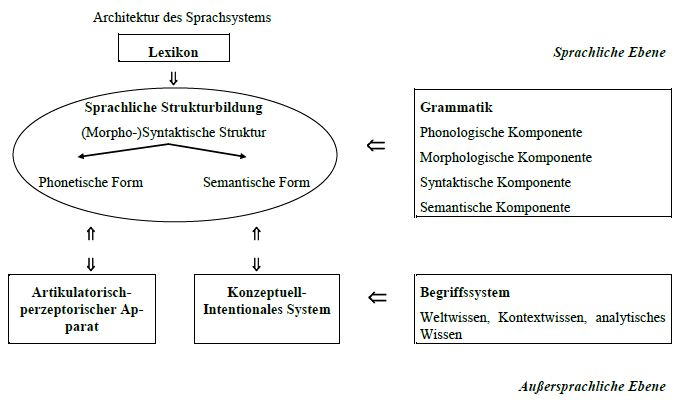
\includegraphics[width=\textwidth]{material/03ArchitekturSprachsystem.jpg}
%	\caption{Architektur des Sprachsystems \citep{Abramowski2016}}
%	\label{Zeichen3}

%\end{figure}

%\end{frame}			


%%%%%%%%%%%%%%%%%%%%%%%%%%%%%%%%%%%
\begin{frame}

\begin{figure}
\centering
\small
\begin{minipage}{0.55\textwidth}
\centering
\fbox{Lexikon}\\
\Large
$ \Downarrow $
\end{minipage}
%
\begin{minipage}{0.1\textwidth}
\centering
\hfill
\end{minipage}
%
\begin{minipage}[t]{0.3\textwidth}
\centering
\textit{Sprachliche Ebene}
\end{minipage}

\begin{minipage}[t]{0.55\textwidth}
\centering
\outputbox{\centering Sprachliche Strukturbildung\\
\begin{forest}sm edges,
[(morpho-)syntaktische Struktur
[Phonetische Form]
[Semantische Form]
]
\end{forest}}
\begin{tabular}{cp{3cm}c}
\Large
$ \Updownarrow $ && \Large $ \Updownarrow $\\
\end{tabular}
\end{minipage}
%
\begin{minipage}[c]{0.1\textwidth}
\centering
\Large
$ \Leftarrow $
\end{minipage}
%
\begin{minipage}[t]{0.3\textwidth}
\centering
\small
\outputbox{
Grammatik
\begin{itemize*}
\item Phonologische Komponente\\
\item Morphologische K.\\
\item Syntaktische K.\\
\item Semantische K.
\end{itemize*}}
\end{minipage}

\begin{minipage}{0.24\textwidth}
\centering
\outputbox{\centering Artikulatorisch-perzeptorischer Apparat}
\end{minipage}
%
\begin{minipage}[c]{0.05\textwidth}
\hfill
\end{minipage}
%
\begin{minipage}{0.24\textwidth}
\centering
\outputbox{\centering Konzeptuell-Intentionales System}
\end{minipage}
%
\begin{minipage}{0.1\textwidth}
\centering
\Large
$\Leftarrow$
\end{minipage}
%
\begin{minipage}{0.3\textwidth}
\outputbox{Begriffssystem
\newline
\small
\raggedright
Weltwissen, Kontextwissen, analytisches Wissen}
\end{minipage}

\begin{minipage}{0.65\textwidth}
\hfill
\end{minipage}
%
\begin{minipage}{0.3\textwidth}
\centering
\small
\textit{Außersprachliche Ebene}
\end{minipage}
\caption{Die Architektur des Sprachsystems \citep[vgl.][]{Abramowski2016}}
\end{figure}

\end{frame}


%%%%%%%%%%%%%%%%%%%%%%%%%%%%%%%%%%%
%%%%%%%%%%%%%%%%%%%%%%%%%%%%%%%%%%%
\subsection{Linguistische Teildisziplinen}		

%% MyP: Contents
\iftoggle{sectoc}{
\frame{
%\begin{multicols}{2}
	\tableofcontents[currentsubsection, subsubsectionstyle=hide]
%\end{multicols}
}
}

%% StM: Contents
\iftoggle{gliederung}{
	
	\outline{
		\begin{itemize}
			
			\item Grammatik
			\item Grammatikbegriff
			\item Modularität der Grammatik
			%% Lexikon
			%% Phonologische Komponente
			%% Morphologische Komponente
			%% Syntaktische Komponente
			%% Semantische Komponente
			%% Architektur des Sprachsystems
			\item \blaubf{Linguistische Teildisziplinen}
			\item Linguistik als Geistes- und/oder Naturwissenschaft
			\item Sprachwissenschaft \vs Linguistik
			
		\end{itemize}
	}
}
%%%%%%%%%%%%%%%%%%%%%%%%%%%%%%%%%%%

\begin{frame}{Linguistische Teildisziplinen}

	\begin{tabular}{ll}
\multirow{4}{*}{im engeren Sinne (System):} & Phonologie \\
																	& Morphologie \\
																	& Syntax \\
																	& Semantik \\
\hline
\multirow{3}{*}{im weiteren Sinne (Gebrauch):} & Phonetik \\
																		& Graphematik \\
																		& Pragmatik \\
\hline
\multirow{5}{*}{Linguistische Methoden:} & Psycholinguistik \\
& Soziolinguistik \\
& Historische Linguistik \\
& Korpuslinguistik \\
& \dots \\
	\end{tabular}
	
\end{frame}



%%%%%%%%%%%%%%%%%%%%%%%%%%%%%%%%%%%
%%%%%%%%%%%%%%%%%%%%%%%%%%%%%%%%%%%
\subsection{Linguistik als Geistes- und/oder Naturwissenschaft}		

%% MyP:Contents
\iftoggle{sectoc}{
\frame{
%\begin{multicols}{2}
	\tableofcontents[currentsubsection, subsubsectionstyle=hide]
%\end{multicols}
}
}

%% StM: Contents
\iftoggle{gliederung}{
	
	\outline{
		\begin{itemize}
			
			\item Grammatik
			\item Grammatikbegriff
			\item Modularität der Grammatik
			%% Lexikon
			%% Phonologische Komponente
			%% Morphologische Komponente
			%% Syntaktische Komponente
			%% Semantische Komponente
			%% Architektur des Sprachsystems
			\item Linguistische Teildisziplinen
			\item \blaubf{Linguistik als Geistes- und/oder Naturwissenschaft}
			\item Sprachwissenschaft \vs Linguistik
			
		\end{itemize}
	}
}
%%%%%%%%%%%%%%%%%%%%%%%%%%%%%%%%%%%

\begin{frame}{Linguistik als Geistes- und/oder Naturwissenschaft}

	\begin{itemize}
		\item \textbf{Geisteswissenschaft}
		
		\begin{itemize}
			\item Verstehen von individuellen Leistungen des Geistes\par
				(eines Menschen, einer Gemeinschaft, einer Epoche)
			\item Verstehen von kulturellen Beziehungen und Entwicklungen
			\item[$\rightarrow$] Methode: \textbf{Hermeneutik} (Annähern durch Verstehen)
		\end{itemize}
		
		\item[]
		\item \textbf{Naturwissenschaft}
		
		\begin{itemize}
			\item Erklärung von naturgesetzlichen Kausalitäten und Zusammenhängen
			\item[$\rightarrow$] Methode: \textbf{Experiment}
		\end{itemize}
		
	\end{itemize}
	
\end{frame}		


%%%%%%%%%%%%%%%%%%%%%%%%%%%%%%%%%%%
\begin{frame}
\frametitle{Linguistik als Naturwissenschaft}

	\begin{itemize}
		\item Linguistik \textit{eher} naturwissenschaftlich ausgerichtet\par
			(im Gegensatz zur Literaturwissenschaft)
		
		\begin{itemize}
			\item[]
			\item \textbf{Beobachtung} und \textbf{Analyse} von Gesetzen natürlicher Sprachen mit dem Ziel ihre \textbf{Systematik} aufzudecken (\zB Syntax)
			\item[]
			\item<2-> Arbeit mit \textbf{empirischen} Verfahren wie Experimenten (\zB Psycholinguistik) oder wie Ansammlungen von Daten (\zB Korpuslinguistik) als Evidenz $\rightarrow$ \textbf{Naturwissenschaft}
			\item[]
			\item<3-> Beschäftigung mit der \textbf{Geschichte} einer Sprache (\zB Historische Linguistik) und mit den \textbf{sozialen} und kulturellen Bedingungen vom Sprachwandel (\zB Soziolinguistik) $\rightarrow$ \textbf{Geisteswissenschaft}
			\item[]
			\item<4-> Untersuchung des vielleicht \textbf{zentralsten Outputs des Geistes}:\par
				der Sprache (vgl. \citealt{Meibauer&Co07a})
		\end{itemize}
		
	\end{itemize}
	
\end{frame}		


%%%%%%%%%%%%%%%%%%%%%%%%%%%%%%%%%%%
%%%%%%%%%%%%%%%%%%%%%%%%%%%%%%%%%%%
\subsection{Sprachwissenschaft \vs Linguistik}

%% MyP: Contents
\iftoggle{sectoc}{
\frame{
%\begin{multicols}{2}
	\tableofcontents[currentsubsection, subsubsectionstyle=hide]
%\end{multicols}
}
}

%% StM: Contents
\iftoggle{gliederung}{
	
	\outline{
		\begin{itemize}
			
			\item Grammatik
			\item Grammatikbegriff
			\item Modularität der Grammatik
			%% Lexikon
			%% Phonologische Komponente
			%% Morphologische Komponente
			%% Syntaktische Komponente
			%% Semantische Komponente
			%% Architektur des Sprachsystems
			\item Linguistische Teildisziplinen
			\item Linguistik als Geistes- und/oder Naturwissenschaft
			\item \blaubf{Sprachwissenschaft \vs Linguistik}
			
		\end{itemize}
	}
}
%%%%%%%%%%%%%%%%%%%%%%%%%%%%%%%%%%%

\begin{frame}{Sprachwissenschaft \vs Linguistik}

	\begin{itemize}
		\item<1-> Linguistik und Sprachwissenschaft werden \idR \textbf{synonymisch} gebraucht.
%		\item[]
		\item<2-> Unterscheidung:
		
		\begin{itemize}
%			\item[]
			\item<2-> Linguistik als \textbf{Teildisziplin} der Sprachwissenschaft
			\item<3-> \gqq{\textbf{Innere Sprachwissenschaft}} $\approx$ Linguistik $\rightarrow$ Beschäftigung mit innersprachlichen Sachverhalten und Entwicklungen (Sprache als System)
			\item<4-> \gqq{\textbf{Äußere Sprachwissenschaft}} $\rightarrow$ Beschäftigung mit kulturellen, sozialen, ökonomischen, politischen, usw. Bedingungen der Existenz und der Geschichte von Sprache, d.\,h. den äußeren (auch \textit{außersprachlich} genannten) Faktoren (vgl. \citealp{Glueck05a})
		\end{itemize}
		
%		\item[]
		\item<5-> In diesem Kurs werden wir jedoch beide Begriffe gleichbedeutend verwenden.
	\end{itemize}
	
\end{frame}

%%%%%%%%%%%%%%%%%%%%%%%%%%%%%%%%%%%

\begin{frame}{Abbildungen}
	\begin{itemize}
		\item ABBILDUNG -- Machicao y Priemer, Antonio: \gqq{Duden} (Privatfoto).
	\end{itemize}
\end{frame}




%%%%%%%%%%%%%%%%%%%%%%%%%%%%%%%%%%%%%%%%%%%%%%%%
%% Compile the master file!
%% 		Include: Antonio Machicao y Priemer
%% 		Course: GK Linguistik
%%%%%%%%%%%%%%%%%%%%%%%%%%%%%%%%%%%%%%%%%%%%%%%%


%%%%%%%%%%%%%%%%%%%%%%%%%%%%%%%%%%%%%%%%%%%%%%%%%%%%
%%%             Metadata                         
%%%%%%%%%%%%%%%%%%%%%%%%%%%%%%%%%%%%%%%%%%%%%%%%%%%%      

\title{Grundkurs Linguistik}

\subtitle{Phonetik}

\author[A. Machicao y Priemer]{
	{\small Antonio Machicao y Priemer}
	\\
	{\footnotesize \url{http://www.linguistik.hu-berlin.de/staff/amyp}}
%	\\
%	{\small\href{mailto:mapriema@hu-berlin.de}{mapriema@hu-berlin.de}}
}

\institute{Institut für deutsche Sprache und Linguistik}

% bitte lassen, sonst kann man nicht sehen, von wann die PDF-Datei ist.
%\date{ }

%\publishers{\textbf{6. linguistischer Methodenworkshop \\ Humboldt-Universität zu Berlin}}

%\hyphenation{nobreak}


%%%%%%%%%%%%%%%%%%%%%%%%%%%%%%%%%%%%%%%%%%%%%%%%%%%%
%%%             Preamble's End                  
%%%%%%%%%%%%%%%%%%%%%%%%%%%%%%%%%%%%%%%%%%%%%%%%%%%%      


%%%%%%%%%%%%%%%%%%%%%%%%%      
\huberlintitlepage[22pt]

\iftoggle{toc}{
\frame{
\begin{multicols}{2}
	\frametitle{Inhaltsverzeichnis}
	\tableofcontents
	%[pausesections]
\end{multicols}
}
}

%%%%%%%%%%%%%%%%%%%%%%%%%%%%%%%%%%
%%%%%%%%%%%%%%%%%%%%%%%%%%%%%%%%%%
%%%%%LITERATURE:

%% Allgemein
\nocite{Glueck&Roedel16a}
\nocite{Schierholz&Co18}
\nocite{Luedeling2009a}
\nocite{Meibauer&Co07a} 
\nocite{Repp&Co15a} 

%%% Sprache & Sprachwissenschaft
%\nocite{Fries16c} %Adäquatheit
%\nocite{Fries16a} %Grammatikalität
%\nocite{Fries&MyP16c} %GG
%\nocite{Fries&MyP16b} %Akzeptabilität
%\nocite{Fries&MyP16d} %Kompetenz vs. Performanz

%% Phonetik & Phonologie
\nocite{Altmann&Co07a}
\nocite{DudenAussprache00a}
\nocite{Hall00a} 
\nocite{Kohler99a}
\nocite{Krech&Co09a}
\nocite{Pompino95a}
\nocite{Ramers08a}
\nocite{Ramers&Vater92a}
\nocite{Rues&Co07a}
\nocite{WieseR11a}


%%%%%%%%%%%%%%%%%%%%%%%%%%%%%%%%%%%
%%%%%%%%%%%%%%%%%%%%%%%%%%%%%%%%%%%
\section{Phonetik}
%%%%%%%%%%%%%%%%%%%%%%%%%%%%%%%%%%%

\begin{frame}
\frametitle{Begleitlektüre}

\begin{itemize}
	\item obligatorisch:
		\begin{itemize}
			\item[] AM S.~7--12
		\end{itemize}
	\item optional:
		\begin{itemize}
			\item[] \citet{Hall00a}: Kapitel 1 (S.~3--16; 19--31)
		\end{itemize}
\end{itemize}

\end{frame}


%%%%%%%%%%%%%%%%%%%%%%%%%%%%%%%%%%%
%%%%%%%%%%%%%%%%%%%%%%%%%%%%%%%%%%%
\subsection{Einführung}

%% MyP: Contents
\iftoggle{sectoc}{
	\frame{
		%\begin{multicols}{2}
		\frametitle{~}
		\tableofcontents[currentsubsection,subsubsectionstyle=hide]
		%\end{multicols}
	}
}

%% StM: Contents
\iftoggle{gliederung}{

\outline{
\begin{itemize}

\item \blaubf{Einführung}
\item Bereiche der Phonetik
\item Methodik
\item Probleme der Phonetik
\item IPA-Alphabet
\item Artikulatorische Phonetik
%% Konsonanten
%% Konsonantenklassikation
%% Vokale
%% Vokalklassifikation
%% Vokalviereck
%% Monophthong, Diphthong, Triphthong
\item Übungen
  
  \end{itemize}
	}
}


%%%%%%%%%%%%%%%%%%%%%%%%%%%%%%%%%%%
\begin{frame}
\frametitle{Einführung}

	\begin{itemize}
		\item Phonetik $\approx$ \gqq{Lautlehre}, \gqq{Lehre der Sprachlaute}, \gqq{Sprechaktlautlehre}
\medskip
		\item Sie beschäftigt sich mit der \textbf{materiellen Seite} des Sprechens $\rightarrow$ \textbf{Sprachlaute}
\medskip
		\item \textbf{Minimaleinheit} der Phonetik:\\
			\textbf{Phon} $\approx$ Sprachlaut $\approx$ Segment $\approx$ einfach nur \gqq{Laut}
\medskip
		\item Sie zählt nicht im engeren Sinne zu den \textit{grammatischen Modulen} in der Sprachkompetenz, sondern zu dem \textbf{artikulatorisch-perzeptorischen Apparat}.
	\end{itemize}
	
\end{frame}


%%%%%%%%%%%%%%%%%%%%%%%%%%%%%%%%%%
\begin{frame}

\begin{figure}
	\centering
	\small
	\begin{minipage}{0.55\textwidth}
		\centering
		\fbox{Lexikon}\\
		\Large
		$ \Downarrow $
	\end{minipage}
	%
	\begin{minipage}{0.1\textwidth}
		\centering
		\hfill
	\end{minipage}
	%
	\begin{minipage}[t]{0.3\textwidth}
		\centering
		\textit{Sprachliche Ebene}
	\end{minipage}
	
	\begin{minipage}[t]{0.55\textwidth}
		\centering
		\outputbox{\centering Sprachliche Strukturbildung\\
			\begin{forest}sm edges,
				[(morpho-)syntaktische Struktur
				[Phonetische Form]
				[Semantische Form]
				]
		\end{forest}}
		\begin{tabular}{cp{3cm}c}
			\Large
			$ \Updownarrow $ && \Large $ \Updownarrow $\\
		\end{tabular}
	\end{minipage}
	%
	\begin{minipage}[c]{0.1\textwidth}
		\centering
		\Large
		$ \Leftarrow $
	\end{minipage}
	%
	\begin{minipage}[t]{0.3\textwidth}
		\centering
		\small
		\outputbox{
			Grammatik
			\begin{itemize*}
				\item Phonologische Komponente\\
				\item Morphologische K.\\
				\item Syntaktische K.\\
				\item Semantische K.
		\end{itemize*}}
	\end{minipage}
	
	\begin{minipage}{0.24\textwidth}
		\centering
		\outputbox{\centering \alertred{Artikulatorisch-perzeptorischer Apparat}}
	\end{minipage}
	%
	\begin{minipage}[c]{0.05\textwidth}
		\hfill
	\end{minipage}
	%
	\begin{minipage}{0.24\textwidth}
		\centering
		\outputbox{\centering Konzeptuell-Intentionales System}
	\end{minipage}
	%
	\begin{minipage}{0.1\textwidth}
		\centering
		\Large
		$\Leftarrow$
	\end{minipage}
	%
	\begin{minipage}{0.3\textwidth}
		\outputbox{Begriffssystem
			\newline
			\small
			\raggedright
			Weltwissen, Kontextwissen, analytisches Wissen}
	\end{minipage}
	
	\begin{minipage}{0.65\textwidth}
		\hfill
	\end{minipage}
	%
	\begin{minipage}{0.3\textwidth}
		\centering
		\small
		\textit{Außersprachliche Ebene}
	\end{minipage}
	\caption{Die Architektur des Sprachsystems \citep[vgl.][]{Abramowski2016}}
\end{figure}

\end{frame}


%%%%%%%%%%%%%%%%%%%%%%%%%%%%%%%%%%%
\begin{frame}
\frametitle{Laute in den Sprachen der Welt}

\begin{itemize}
	\item Insgesamt zählt man über \textbf{200 Vokale} und über \textbf{500 Konsonanten}.
	
		\begin{itemize}
			\item Pirahã (Amazonas): 10 Laute (eher Phoneme)\\
				\textbf{VIDEO:} \href{run:material/04SpokenPiraha.mp4}{Spoken Pirahã with subtitles}
			\item Hawaiianisch: 11--13 Laute (eher Phoneme)
			\item {!}Xóõ (Botswana, Namibia): 141--159 Laute (eher Phoneme)
			\item Deutsch: 50 Laute (ung. 32 Phoneme)
		\end{itemize}
		
\end{itemize}
	
\end{frame}


%%%%%%%%%%%%%%%%%%%%%%%%%%%%%%%%%%
\begin{frame}
\frametitle{Übung}

Wie viele Laute haben die folgenden Wörter?

\begin{enumerate}
	\item \ab{Fische}
	\item \ab{Nixe}
	\item \ab{lang}
	\item \ab{Bearbeitung}
\end{enumerate}
\end{frame}


%%%%%%%%%%%%%%%%%%%%%%%%%%%%%%%%%%%
\iftoggle{ue-loesung}{

	%%%%%%%%%%%%%%%%%%%%%%%%%%%%%%%%%%
%% UE 1 - 02 Phonetik
%%%%%%%%%%%%%%%%%%%%%%%%%%%%%%%%%%

\begin{frame}
\frametitle{Übung -- Lösung}

Wie viele Laute haben die folgenden Wörter?

\begin{columns}
	\column{.30\textwidth}
	\begin{enumerate}
		\item \ab{Fische}
		\item \ab{Nixe}
		\item \ab{lang}
		\item \ab{Bearbeitung}
		\item[]
	\end{enumerate} 				
	\column{.35\textwidth}
	\begin{enumerate}
		\item<1-> \alertgreen{\textipa{[ f \textsci{} \textesh{} @ ]}}
		\item<3-> \alertgreen{\textipa{[ n \textsci{} k s @ ]}}
		\item<5-> \alertgreen{\textipa{[ l a N ]}}
		\item<7-> \alertgreen{\textipa{[ b @ P a \textscr\  b \t{aI} t U N ]}}
		\item<9->[] \alertgreen{\textipa{[ b @ P a:  b \t{aI} t U N ]}}
	\end{enumerate} 
	\column{.15\textwidth}
	\begin{enumerate}
		\item<2->[] \alertgreen{4}
		\item<4->[] \alertgreen{5}
		\item<6->[] \alertgreen{3}
		\item<8->[] \alertgreen{10--11} % bearbeitung ai als ein
		% Laut oder als zwei gezählt
		\item<10->[] \alertgreen{9--10} % beabeitung ai als ein
		% Laut oder als zwei gezählt
	\end{enumerate}
\end{columns}


\bigskip
\begin{itemize}
	\item[]<11-> \alertgreen{\textipa{[\t{aI}]} kann man als einen oder als zwei Laute zählen.}
\end{itemize}         

\end{frame}


}
%%%%%%%%%%%%%%%%%%%%%%%%%%%%%%%%%%%


%%%%%%%%%%%%%%%%%%%%%%%%%%%%%%%%%%%
\begin{frame}
\frametitle{Einordnung der Phonetik als Wissenschaft}

\begin{itemize}

	\item Methodik: \textbf{naturwissenschaftlich}
\medskip
	\item Messung und Analyse physiologischer und physikalischer Aspekte der Sprache
\medskip
	\item \textbf{Lautkontinuum} wird in einzelne Laute zerlegt
\medskip
	\item Bereiche der Phonetik:

	\begin{itemize}
		\item Artikulatorische Phonetik
		
		\item Akustische Phonetik
		
		\item Auditive (perzeptive) Phonetik
	\end{itemize}
	
\end{itemize}

\end{frame}


%%%%%%%%%%%%%%%%%%%%%%%%%%%%%%%%%%%
%%%%%%%%%%%%%%%%%%%%%%%%%%%%%%%%%%%
\subsection{Bereiche der Phonetik}

%% MyP: Contents
\iftoggle{sectoc}{
	\frame{
		%\begin{multicols}{2}
		\frametitle{~}
		\tableofcontents[currentsubsection,subsubsectionstyle=hide]
		%\end{multicols}
	}
}

%% StM: Contents
\iftoggle{gliederung}{
\outline{

\begin{itemize}

\item Einführung
\item \blaubf{Bereiche der Phonetik}
  \item  Methodik
\item  Probleme der Phonetik
\item  IPA-Alphabet
\item Artikulatorische Phonetik
%% Konsonanten
%% Konsonantenklassifikation
%% Vokale
%% Vokalklassifikation
%% Vokalviereck
%% Monophthong, Diphthong, Triphthong
\item Übungen
  
  \end{itemize}
	}
}


%%%%%%%%%%%%%%%%%%%%%%%%%%%%%%%%%%%
\begin{frame}{Bereiche der Phonetik}

	\begin{table}
	\centering 
	
		\begin{tabular}{p{0.23\linewidth}p{0.05\linewidth}p{0.23\linewidth}p{0.05\linewidth}p{0.23\linewidth}}
			\hline
			\textbf{Artikulatorische Phonetik} & & \textbf{Akustische}\par \textbf{Phonetik} & & \textbf{Auditive}\par \textbf{Phonetik} \\
			\hline
  			Sprecher & & Schallsignal & & Hörer \\
			\hline
			Lautproduktion & $\rightarrow$ & Transmission & $\rightarrow$ & Perzeption\\
			\hline
		\end{tabular}
		
	\caption{Bereiche der Phonetik \citep{Ramers08a}} 
	\end{table}	
		
\end{frame}


%%%%%%%%%%%%%%%%%%%%%%%%%%%%%%%%%%%
\begin{frame}
\frametitle{Bereiche der Phonetik}

	\begin{itemize}
		\item \textbf{Artikulatorische Phonetik}
		
\textbf{Erzeugung} von Lautereignissen (von der Steuerung durch das Gehirn bis zu den konkreten artikulatorischen Bewegungen im Mund-, Rachen- und Nasenraum und im Kehlkopf)

			\ea Zungenbewegung bei der Aussprache des Lautes \textipa{[ \texttoptiebar{tS} ]}
			\z

\pause 
		
		\item \textbf{Akustische Phonetik}
		
                       physikalische Eigenschaften von \textbf{Schallwellen},\\
                       die bei der Produktion und Übertragung von Sprachlauten auftreten

			\ea physikalische Eigenschaften eines Lauts im Übertragungsprozess: Frequenzbereich, Intensität, Länge, etc.
			\z

	\end{itemize}

\end{frame}


%%%%%%%%%%%%%%%%%%%%%%%%%%%%%%%%%%%
\begin{frame}
\frametitle{Bereiche der Phonetik}

\begin{itemize}

			
		\item \textbf{Auditive (perzeptive) Phonetik}
		
		      \textbf{Wahrnehmung} (Empfang und Verstehen) von Sprachlauten

			\ea Wie nimmt der Hörer den Unterschied zwischen den Vokalen in \ab{Beet} und \ab{Bett} wahr?
			\z
		
	\end{itemize}
	
\end{frame}


%%%%%%%%%%%%%%%%%%%%%%%%%%%%%%%%%%%
%%%%%%%%%%%%%%%%%%%%%%%%%%%%%%%%%%%
\subsection{Methodik}

%% MyP: Contents
\iftoggle{sectoc}{
	\frame{
		%\begin{multicols}{2}
		\frametitle{~}
		\tableofcontents[currentsubsection,subsubsectionstyle=hide]
		%\end{multicols}
	}
}

%% StM: Contents
\iftoggle{gliederung}{
\outline{

\begin{itemize}

\item Einführung
\item Bereiche der Phonetik
\item \blaubf{Methodik}
\item Probleme der Phonetik
\item IPA-Alphabet
\item Artikulatorische Phonetik
%% Konsonanten
%% Konsonantenklassifikation
%% Vokale
%% Vokalklassifikation
%% Vokalviereck
%% Monophthong, Diphthong, Triphthong
\item Übungen
  
  \end{itemize}
	}
}


%%%%%%%%%%%%%%%%%%%%%%%%%%%%%%%%%%%
\begin{frame}{Methodik}

	\begin{figure}
		\centering
		
		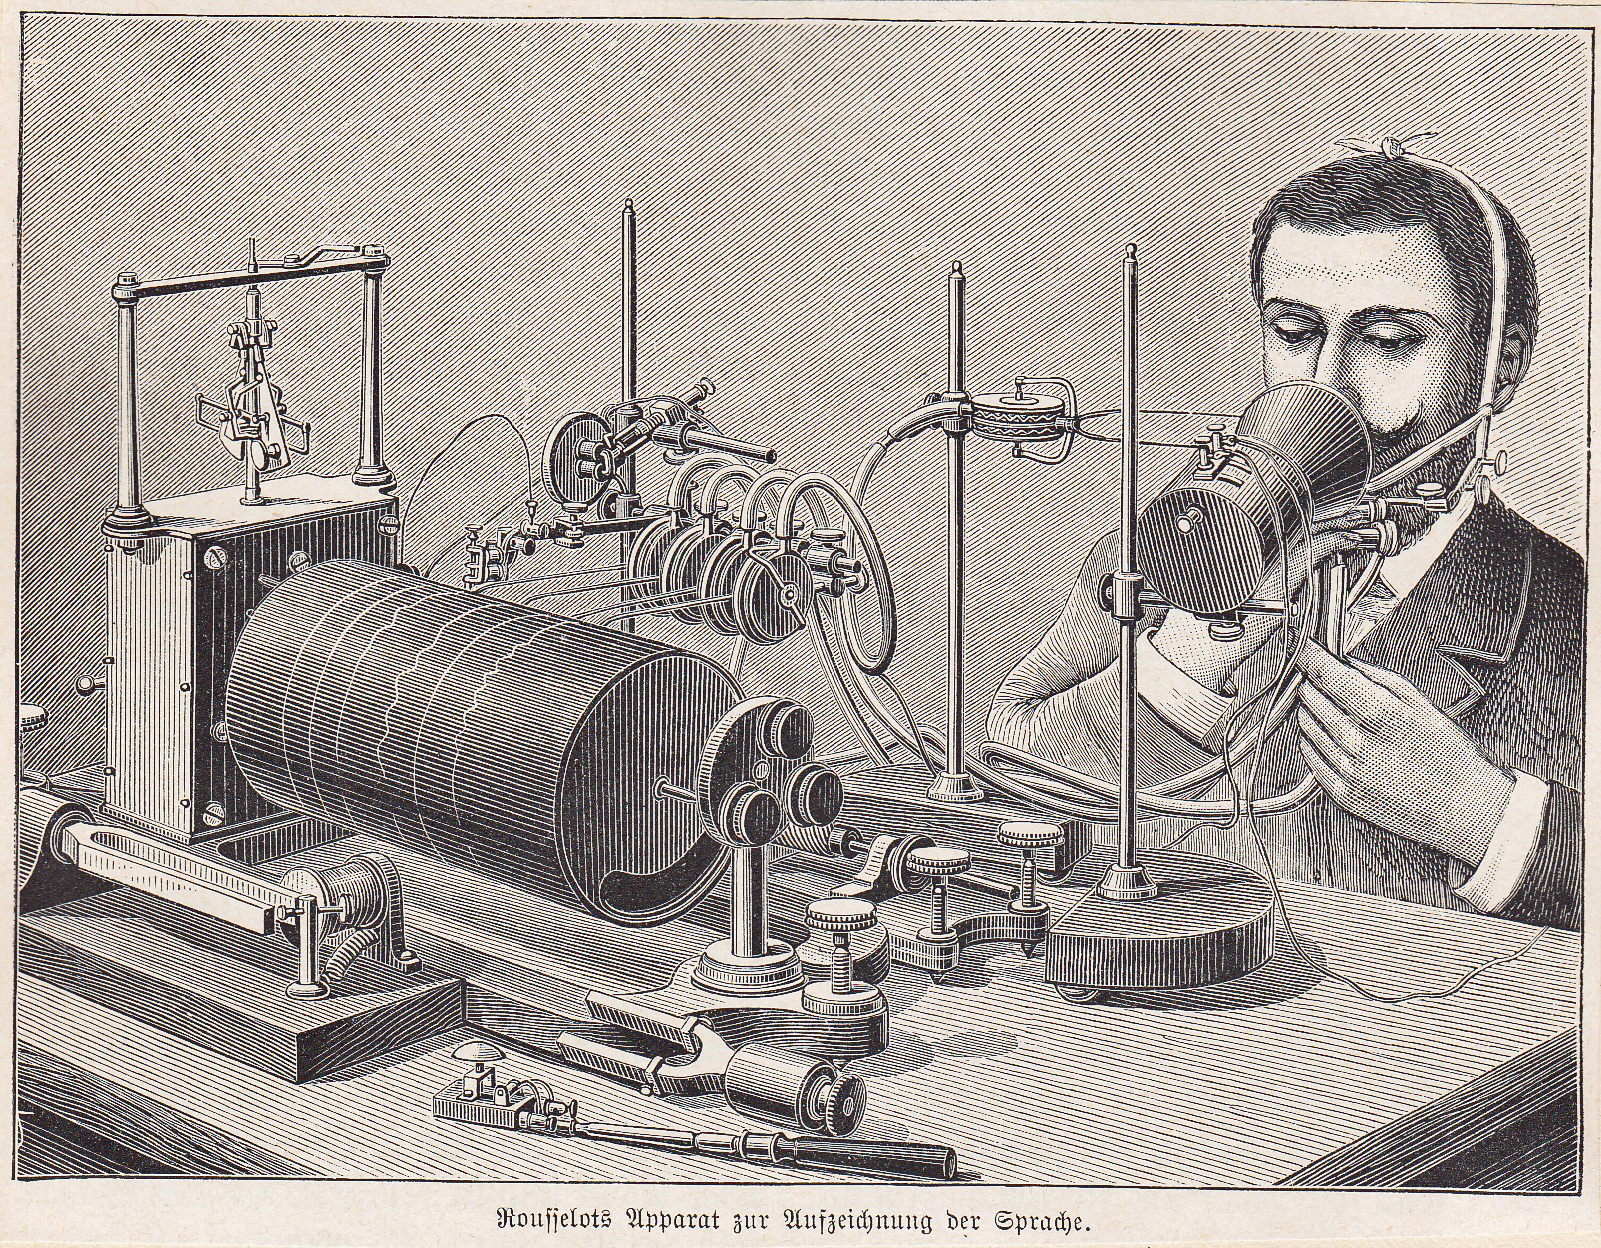
\includegraphics[scale=0.1]{material/04RousselotsApparatzurAufzeichnungderSprache}
		\caption{Rousselots Apparat}
		%{material/04proband}
		%\caption{Proband \citep{Pompino95a}}
		%\label{Zeichen1}
	\end{figure}
	
\end{frame}


%%%%%%%%%%%%%%%%%%%%%%%%%%%%%%%%%%%
%Alternative:

%\begin{frame}{Methodik}

%	\begin{figure}[H]
%		\centering
		
%		\includegraphics[scale=0.07]{material/04Rousselots_Apparat_zu_Aufzeichnung_der_Sprache}
%		\caption{Rousselots Apparat, gemeinfrei, Quelle: Museum für Kommunikation Frankfurt, https://de.wikipedia.org/wiki/Datei:Rousselots_Apparat_zur_Aufzeichnung_der_Sprache.jpg}
		%\label{Zeichen1}
%	\end{figure}
	
%\end{frame}


%%%%%%%%%%%%%%%%%%%%%%%%%%%%%%%%%%%
\begin{frame}
\frametitle{Deskriptive, Symbol-, Instrumental- und Signalphonetik}

	\begin{itemize}
		\item Der geschulte Ohrenphonetiker analysiert und beschreibt das Gehörte
                  (\textbf{deskriptive Phonetik}).

                  Die analysierten Lautkategorien werden anschließend mit symbolischen Mitteln (dem Internationalen Phonetischen Alphabet -- IPA) dargestellt (\textbf{Symbolphonetik}).

		\item Phonetiker nehmen die ablaufenden physikalischen Vorgänge mittels spezieller Mess- oder Registriergeräte während des Sprechaktes als Signale auf (\textbf{Instrumental-} oder \textbf{Signalphonetik}).
	\end{itemize}
	
\end{frame}


%%%%%%%%%%%%%%%%%%%%%%%%%%%%%%%%%%%
\begin{frame}
\frametitle{Methodik: Beispiele}

Messen/Erfassen von
	\begin{itemize}
\item Kiefer-, Lippen- und Zungenbewegungen mithilfe der elektrischen Muskelpotenziale
\item Luftdruckschwankungen, die das akustische Signal darstellen
\item Verlauf des intraoralen Luftdrucks
\item Veränderung der Durchblutung bestimmter Großhirnregionen bei der Verarbeitung von lautsprachlichen Reizen
	\end{itemize}	
\end{frame}


%%%%%%%%%%%%%%%%%%%%%%%%%%%%%%%%%%%
\begin{frame}
\frametitle{Zusammenhang zwischen Experimental- und perzeptiver Phonetik}

	\begin{itemize}
		\item \textbf{Experimentalphonetik} oder \textbf{perzeptive Phonetik} untersucht den
                  Zusammenhang zwischen bestimmten Signalausprägungen und der Wahrnehmung von Versuchspersonen.

                  Damit wird ein Zusammenhang zwischen der Instrumentalphonetik und der deskriptiven Phonetik erzeugt.
	\end{itemize}
	
	\ea	Bei Veränderung von einzelnen akustischen Parametern:\\
	Ab wann nimmt eine Versuchsperson ein \textipa{[ da ]} als \textipa{[ ta ]} wahr?
	\z 
	
\end{frame}


%%%%%%%%%%%%%%%%%%%%%%%%%%%%%%%%%%%
%%%%%%%%%%%%%%%%%%%%%%%%%%%%%%%%%%%
\subsection{Probleme der Phonetik}

%% MyP: Contents
\iftoggle{sectoc}{
	\frame{
		%\begin{multicols}{2}
		\frametitle{~}
		\tableofcontents[currentsubsection,subsubsectionstyle=hide]
		%\end{multicols}
	}
}

%% StM: Contents
\iftoggle{gliederung}{
\outline{

\begin{itemize}

\item Einführung
\item Bereiche der Phonetik
\item  Methodik
\item  \blaubf{Probleme der Phonetik}
\item  IPA-Alphabet
\item Artikulatorische Phonetik
%% Konsonanten
%% Konsonantenklassifikation
%% Vokale
%% Vokalklassifikation
%% Vokalviereck
%% Monophthong, Diphthong, Triphthong
\item Übungen
  
  \end{itemize}
	}
}


%%%%%%%%%%%%%%%%%%%%%%%%%%%%%%%%%%%
\begin{frame}{Probleme der Phonetik: schnelle Übermittlung der Laute}

\begin{itemize}
	\item kurzer Satz (mit 50 Segmenten): ung. 2 Sekunden\\
		\dash bis zu 25 (sprachliche) Segmente pro Sekunde
\medskip
	\item nicht-sprachliche Segmente: ung. 7 bis 9 pro Sekunde
	\item[\ra] Hohe Geschwindigkeit bei der Äußerung eines Satzes macht aus einer sprachlichen Äußerung ein \textbf{Kontinuum}, in dem die Segmentierung der Laute besonders schwer ist.
\end{itemize}


\end{frame}


%%%%%%%%%%%%%%%%%%%%%%%%%%%%%%%%%%%
\begin{frame}
\frametitle{Schallsignal als Kontinuum}

	\begin{figure}[H]
	\centering
	
	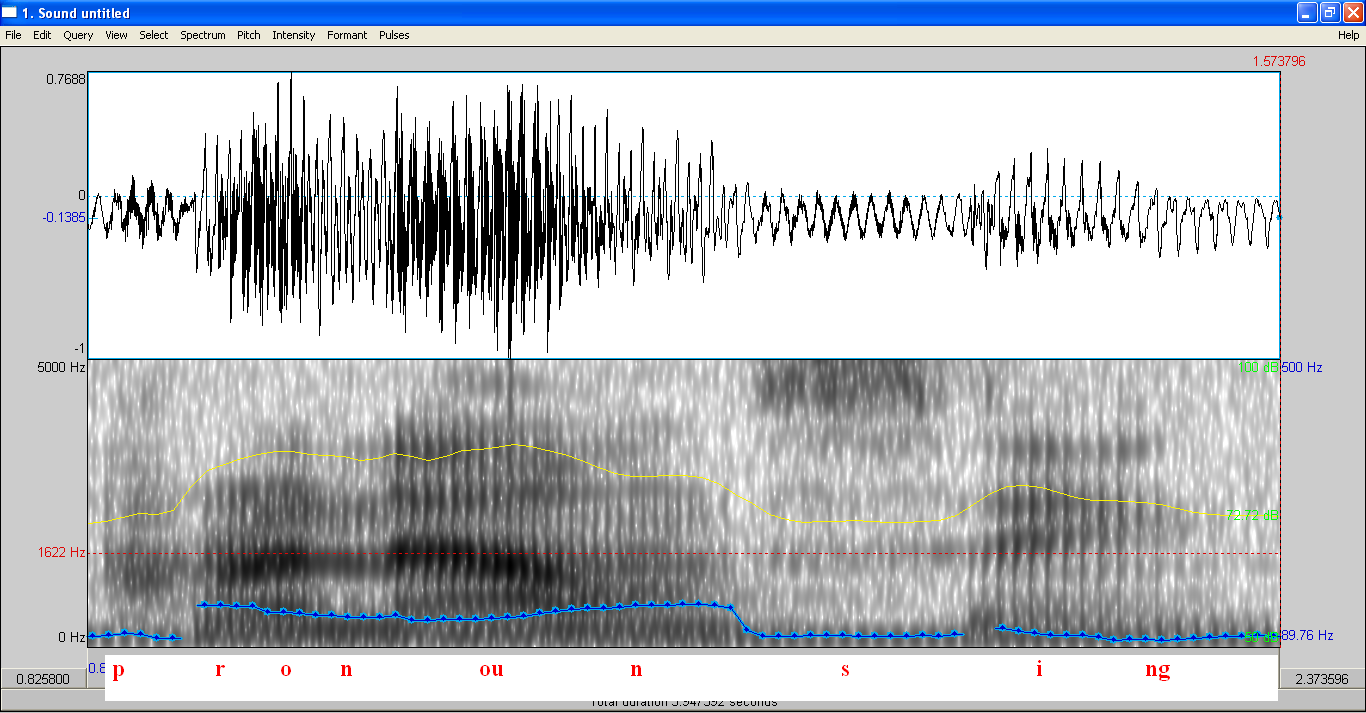
\includegraphics[scale=0.2]{material/04Pronouncing}
	\caption{Spektrogramm des Wortes \emph{pronouncing}}
	%Die alte Version: \includegraphics[scale=0.50]{material/oszillogrammwiese} \caption{\citep{WieseR11a}}
	%\label{Zeichen1}
	\end{figure}

Schallsignal ist ein Kontinuum, eine genaue Segmentierung daher schwierig
	
\end{frame}


%%%%%%%%%%%%%%%%%%%%%%%%%%%%%%%%%%%
\begin{frame}
\frametitlefit{Keine 1-zu-1-Korrespondenz zw.\ Lauten und Verschriftlichung}

\begin{itemize}
			
	\item ein Laut \ras mehrere Buchstaben

	\ea \textipa{[s]} \ras \ab{\textbf{S}maragd}, \ab{gro\textbf{ß}}, \ab{e\textbf{ss}en}
	\z
	
	
	\item eine Buchstabenfolge \ras unterschiedliche Laute

	\ea \ab{ch} \ras \ab{mi\textbf{ch}}, \ab{Bu\textbf{ch}}, \ab{se\textbf{ch}s}, \ab{\textbf{Ch}arme}, \ab{\textbf{Ch}ip}
	\z
	
\end{itemize}

\medskip

\begin{description}
	\item[\textbf{IPA-Alphabet:}] Schriftsystem mit 1-zu-1-Korrespondenz zwischen Lauten und (diakritischen) Zeichen
\end{description}	
		
\end{frame}


%%%%%%%%%%%%%%%%%%%%%%%%%%%%%%%%%%%
%%%%%%%%%%%%%%%%%%%%%%%%%%%%%%%%%%%
\subsection{IPA-Alphabet}

%% MyP: Contents
\iftoggle{sectoc}{
	\frame{
		%\begin{multicols}{2}
		\frametitle{~}
		\tableofcontents[currentsubsection,subsubsectionstyle=hide]
		%\end{multicols}
	}
}

%%StM: Contents
\iftoggle{gliederung}{

\outline{

\begin{itemize}

\item Einführung
\item Bereiche der Phonetik
\item  Methodik
\item  Probleme der Phonetik
\item  \blaubf{IPA-Alphabet}
\item Artikulatorische Phonetik
%% Konsonanten
%% Konsonantenklassifikation
%% Vokale
%% Vokalklassifikation
%% Vokalviereck
%% Monophthong, Diphthong, Triphthong
\item Übungen
  
  \end{itemize}
	}
}


%%%%%%%%%%%%%%%%%%%%%%%%%%%%%%%%%%%
\begin{frame}{IPA-Alphabet}

	\begin{itemize}
		\item IPA: International Phonetic Association \ras IPA-Alphabet
		\item Seit Mitte des 19. Jh. \ras Entwicklung von phonetischen Umschriftsystemen
		\item IPA-Alphabet ist das am weitesten verbreitete System.
		\item Alle Sprachlaute aller natürlichen Sprachen werden eindeutig dargestellt (phonetische Transkription).
\medskip
		\item \textbf{Repräsentation der Phone} \ras in eckigen Klammern \gqq{\textipa{[ ]}}
		\item \textbf{Orthographische Repräsentation} \ras in spitzen Klammern \gqq{$\langle{} \rangle{}$}
\medskip
		\item {Webseite der IPA}: \url{http://internationalphoneticassociation.org}
		\item {Laute zum Testen}: \url{http://www.ipachart.com/}
	\end{itemize}
	
\end{frame}


%%%%%%%%%%%%%%%%%%%%%%%%%%%%%%%%%%%
%\begin{frame}
%\frametitle{IPA-Alphabet}
%
%	\begin{figure}[H]
%		\centering
%		
%		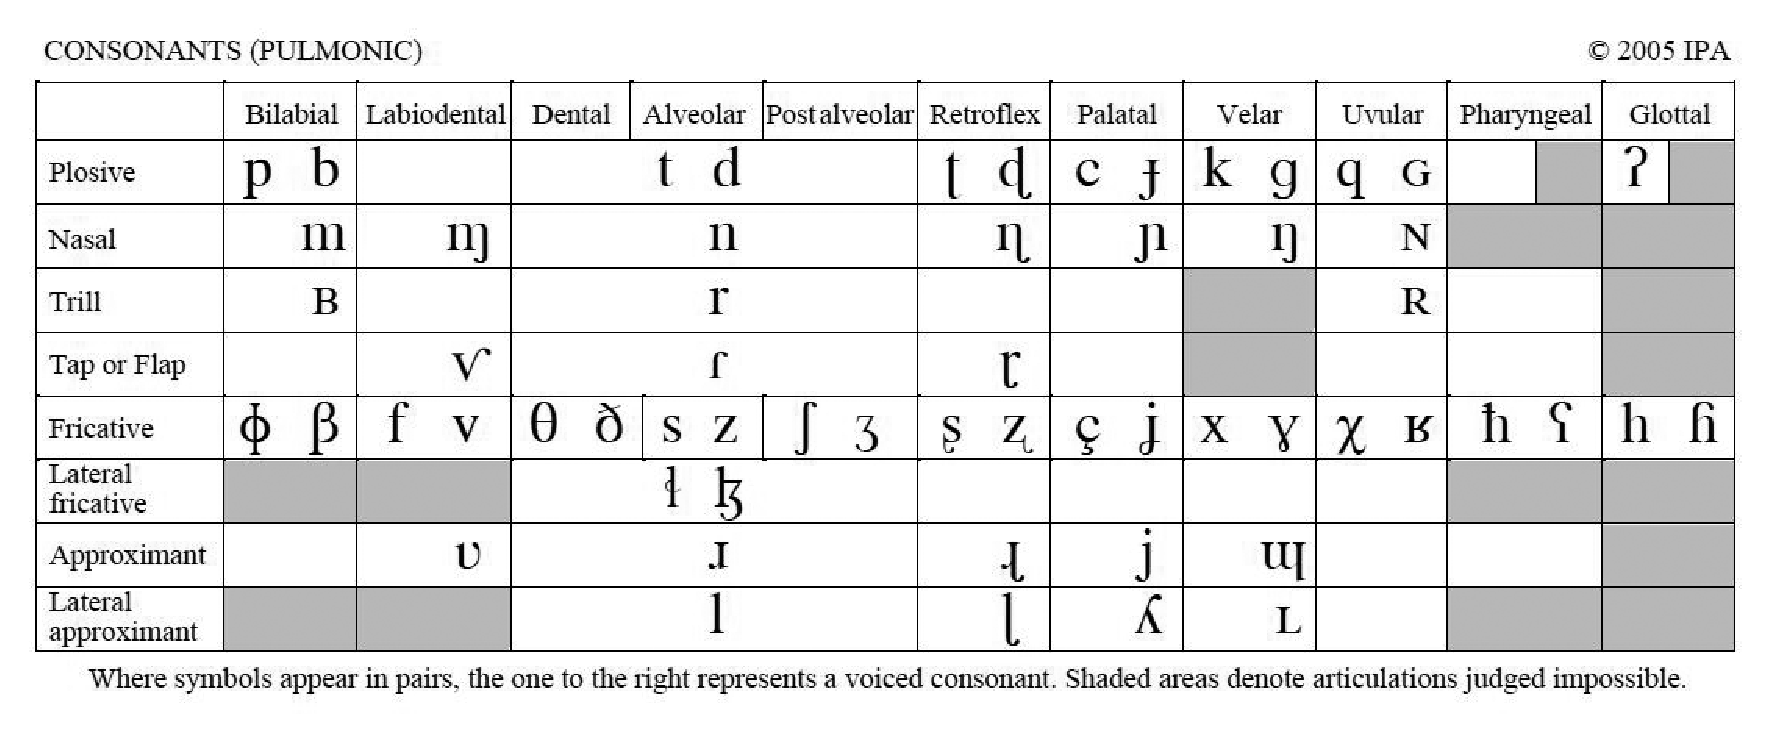
\includegraphics[scale=0.35]{material/04ipaconsonantpulmonic}
%		\caption{Konsonanten (Pulmonal)}
%		%\label{Zeichen1}
%	\end{figure}	
%	
%\end{frame}


%%%%%%%%%%%%%%%%%%%%%%%%%%%%%%%%%%%
\begin{frame}
\frametitle{Pulmonale Konsonanten im IPA-Alphabet}

\begin{table}
\centering
\begin{adjustbox}{max width=\textwidth}
\begin{tabular}{|p{0.1\textwidth}|c|c|c|c|c|c|c|c|c|c|c|c|c|}
\hline
& \tiny{Bilabial} & \tiny{Labiodental} & \tiny{Dental} & \tiny{Alveolar} & \tiny{Postalveolar} & \tiny{Retroflex} & \tiny{Palatal} & \tiny{Velar} & \tiny{Uvular} & \multicolumn{2}{|c|}{\tiny{Pharyngal}} & \multicolumn{2}{|c|}{\tiny{Glottal}} \\
\hline
\tiny{Plosive} & \textipa{p b} & & \multicolumn{3}{|c|}{\textipa{t d}} & \textipa{\:d \:t} & \textipa{c \textbardotlessj} & \textipa{k g} & \textipa{q \textscg} &  & \cellcolor{lightgray} & \textipa{P} & \cellcolor{lightgray} \\
\hline
\tiny{Nasale} & \textipa{m} & \textipa{\textltailm} & \multicolumn{3}{|c|}{\textipa{n}} & \textipa{\textrtailn} & \textipa{\textltailn} & \textipa{\ng} & \textipa{\textscn} & \multicolumn{2}{|c|}{\cellcolor{lightgray}} & \multicolumn{2}{|c|}{\cellcolor{lightgray}} \\
\hline
\tiny{Vibranten} & \textipa{\textscb} & & \multicolumn{3}{|c|}{\textipa{r}} & & & \cellcolor{lightgray} & \textipa{\textscr} & \multicolumn{2}{|c|}{} & \multicolumn{2}{|c|}{\cellcolor{lightgray}} \\
\hline
\tiny{Taps/ Flaps} & & &  \multicolumn{3}{|c|}{\textipa{\textfishhookr}} &  \textipa{\textrtailr} & & \cellcolor{lightgray} & & \multicolumn{2}{|c|}{} & \multicolumn{2}{|c|}{\cellcolor{lightgray}} \\
\hline
\tiny{Frikative} & \textipa{\textphi \textbeta} & \textipa{f v} & \textipa{\texttheta \dh} & \textipa{s z} & \textipa{S Z} & \textipa{\:s \:z} & \textipa{\c{c} J} & \textipa{x G} & \textipa{X \textinvscr} & \multicolumn{2}{|c|}{\textipa{\textcrh \textrevglotstop}} & \multicolumn{2}{|c|}{\textipa{h \texthth}} \\
\hline
\tiny{Laterale Frikative} & \cellcolor{lightgray} & \cellcolor{lightgray} & \multicolumn{3}{|c|}{\textipa{\textbeltl \textlyoghlig}} & & & & &  \multicolumn{2}{|c|}{\cellcolor{lightgray}} & \multicolumn{2}{|c|}{\cellcolor{lightgray}} \\
\hline
\tiny{Approximanten} & & \textipa{\textscriptv} & \multicolumn{3}{|c|}{\textipa{\textturnr}} & \textipa{\:R} & \textipa{j} & \textipa{\textturnmrleg} & & \multicolumn{2}{|c|}{} & \multicolumn{2}{|c|}{\cellcolor{lightgray}} \\
\hline
\tiny{Laterale Approximanten} & \cellcolor{lightgray} & \cellcolor{lightgray} & \multicolumn{3}{|c|}{\textipa{l}} & \textipa{\:l} & \textipa{\textturny} & \textipa{\textscl} & & \multicolumn{2}{|c|}{\cellcolor{lightgray}} & \multicolumn{2}{|c|}{\cellcolor{lightgray}} \\
\hline
\end{tabular}
\end{adjustbox}
%\caption{Pulmonische Konsonanten, IPA. Bei Paaren ist der rechte Konsonant stimmhaft. Graue Flächen gelten als artikulatorisch unmöglich.
	 %https://www.internationalphoneticassociation.org/sites/default/files/pulmonic.gif Stand: 09.12.16
% } 
\end{table}

\begin{itemize}
\item Bei Paaren ist der rechte Konsonant stimmhaft.
\item Graue Flächen gelten als artikulatorisch unmöglich.
\item Achtung: Affrikaten sind hier nicht verzeichnet!
\end{itemize}
  
\end{frame}


%%%%%%%%%%%%%%%%%%%%%%%%%%%%%%%%%%%
\begin{frame}
\frametitle{Nichtpulmonale Konsonanten im IPA-Alphabet}

\begin{table}
	\centering
	\begin{adjustbox}{max width=\textwidth}
		\begin{tabular}{|c c | c c | c c|}
			\hline
			\multicolumn{2}{|c|}{Clicks} & \multicolumn{2}{|c|}{Voiced implosives} & \multicolumn{2}{|c|}{Ejectives} \\
			\hline
			\textipa{\!o} & \tiny{Bilabial} & \textipa{\!b} & \tiny{Bilabial} &  \textipa{'} & \\
			\textipa{\textpipe} & \tiny{Dental} & \textipa{\!d} & \tiny{Dental/alveolar} & \textipa{p'} & \tiny{Bilabial} \\
			\textipa{!} & \tiny{(Post)alveolar} & \textipa{\!j} & \tiny{Palatal} & \textipa{t'} & \tiny{Dental/alveolar} \\
			\textipa{\textdoublebarpipe} & \tiny{Palatoalveolar} & \textipa{\!g} & \tiny{Velar} & \textipa{k'} & \tiny{Velar} \\
			\textipa{\textdoublepipe} & \tiny{Alveolar lateral} & \textipa{\!G} & \tiny{Uvular} & \textipa{s'} & \tiny{Alveolar frikativ} \\
			\hline
		\end{tabular}
	\end{adjustbox}
%	\caption{Nichtpulmonale Konsonanten, IPA.
		%https://www.internationalphoneticassociation.org/sites/default/files/pulmonic.gif Stand: 09.12.16
%	} 
\end{table}

%	\begin{figure}[H]
%		\centering
%		
%		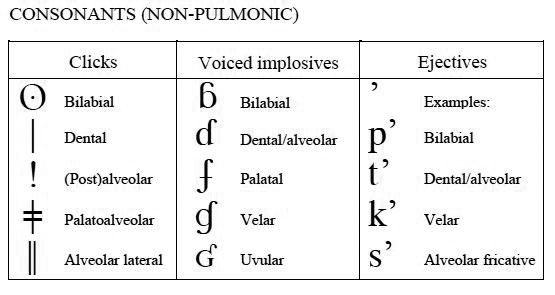
\includegraphics[scale=0.45]{material/04ipaconsonantnonpulmonic}
%		\caption{Konsonanten (Nicht Pulmonal)}
%		%\label{Zeichen1}
%	\end{figure}
	
	\begin{itemize}
		\item \textbf{VIDEO:} \href{run:material/04namaclicks.mp4}{!Nama Clicks}
	\end{itemize}
			
\end{frame}


%%%%%%%%%%%%%%%%%%%%%%%%%%%%%%%%%%%
\begin{frame}
\frametitle{Vokale im IPA-Alphabet: das Vokalviereck}

%	\begin{figure}[H]
%		\centering
%		
%		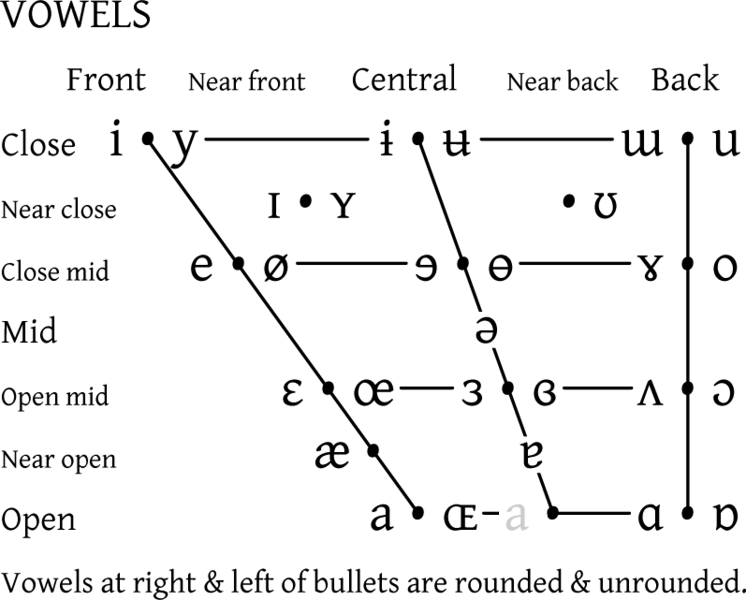
\includegraphics[scale=0.27]{material/04ipavowelwikicommons}
%		\caption{Vokale}
%		%old picture
%		%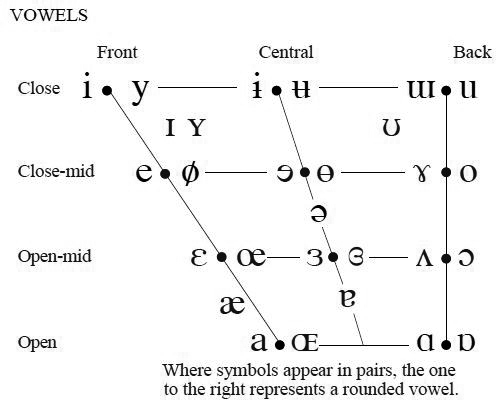
\includegraphics[scale=0.45]{material/04ipavowel}
%		%\caption{Vokale}
%		%\label{Zeichen1}
%	\end{figure}


\centerline{
	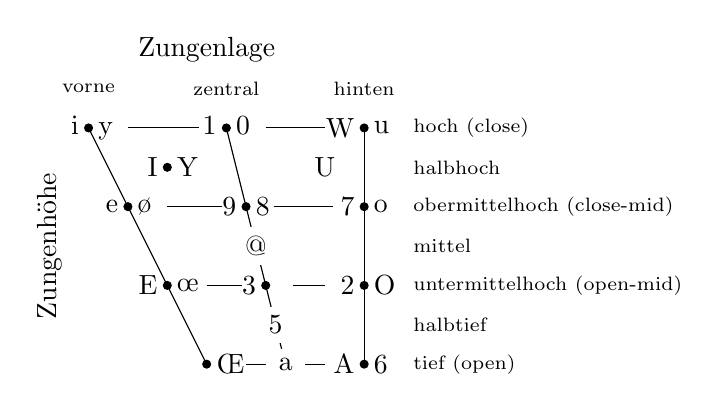
\begin{tikzpicture}
	\draw[fill] (0,0) circle [radius=0.05];
	\draw[fill] (-0.5,1) circle [radius=0.05];
	\draw[fill] (-1,2) circle [radius=0.05];
	\draw[fill] (-1.5,3) circle [radius=0.05];
	\draw[black] (0.5,0)--(0.75,0);
	\draw[black] (1.25,0)--(1.5,0);
	\draw[fill] (2,0) circle [radius=0.05];
	\draw[fill] (2,1) circle [radius=0.05];
	\draw[fill] (2,2) circle [radius=0.05];
	\draw[fill] (2,3) circle [radius=0.05];
	\draw[fill] (0.25,3) circle [radius=0.05];
	\draw[black] (0.25,3)--(1,0);
	\draw[black] (-0.1,3)--(-1,3);
	\draw[black] (0.75,3)--(1.5,3);
	\draw[fill] (0.5,2) circle [radius=0.05];
	\draw[fill] (0.75,1) circle [radius=0.05];
	\node[right] at (0.25,3){\strut \textipa{0}};
	\node[left] at (0.25,3){\strut \textipa{1}};
	\node at (0,4){Zungenlage};
	\node [rotate=90] at (-2,1.5){Zungenhöhe};
	\node at (-1.5,3.5){{\scriptsize vorne}};
	\node at (0.25,3.5){\scriptsize zentral};
	\node at (2,3.5){{\scriptsize hinten}};
	\node[right] at (2.5,3){\scriptsize hoch (close)};
	\node[right] at (2.5,2.5){\scriptsize halbhoch};
	\node[right] at (2.5,2){\scriptsize obermittelhoch (close-mid)};
	\node[right] at (2.5,1.5){\scriptsize mittel};
	\node[right] at (2.5,1){\scriptsize untermittelhoch (open-mid)};
	\node[right] at (2.5,0.5){\scriptsize halbtief};
	\node[right] at (2.5,0){\scriptsize tief (open)};
	\node[left] at (2,3){\textipa{W}};
	\node[right] at (2,3){\textipa{u}};
	\node at (1.5,2.5){\textipa{U}};
	\node[left] at (2,2){\textipa{7}};
	\node[right] at (2,2){\textipa{o}};
	\node[left] at (2,1){\textipa{2}};
	\node[right] at (2,1){\textipa{O}};
	\node[right] at (2,0){\textipa{6}};
	\node[left] at (2,0){\textipa{A}};
	\draw[black] (2,0)--(2,3);
	\node[left] at (0.5,2){\textipa{9}};
	\node[right] at (0.5,2){\textipa{8}};
	\node[rectangle,fill=white] at (0.625,1.5){\textipa{@}};
	\node[left] at (0.75,1){\textipa{3}};
	\node[right] at (0.75,1){\textipa{\textcloserevepsilon}};
	\node[rectangle,fill=white] at (0.875,0.5){\textipa{5}};
	\node[rectangle,fill=white] at (1,0){\textipa{a}};
	\node[right] at (-1.5,3){\strut \textipa{y}};
	\node[left] at (-1.5,3){\strut \textipa{i}};
	\node[left] at (-0.5,2.5){\textipa{I}};
	\node[right] at (-0.5,2.5){\textipa{Y}};
	\draw[fill] (-0.5,2.5) circle [radius=0.05];
	\node[right] at (-1,2){\textipa{\o}};
	\node[left] at (-1,2){\textipa{e}};
	\node[right] at (-0.5,1){\textipa{\oe}};
	\node[left] at (-0.5,1){\textipa{E}};
	\node[right] at (0,0){\textipa{\OE}};
	\draw[black] (0,0)--(-1.5,3);
	\draw[black] (-0.5,2)--(0.2,2);
	\draw[black] (0.85,2)--(1.6,2);
	\draw[black] (0,1)--(0.45,1);
	\draw[black] (1.1,1)--(1.5,1);
	\end{tikzpicture}
}
        
        Vokale links des Punktes sind ungerundet,\\
        die rechts sind gerundet.

%=======
%	\begin{figure}[H]
%		\centering
%		
%		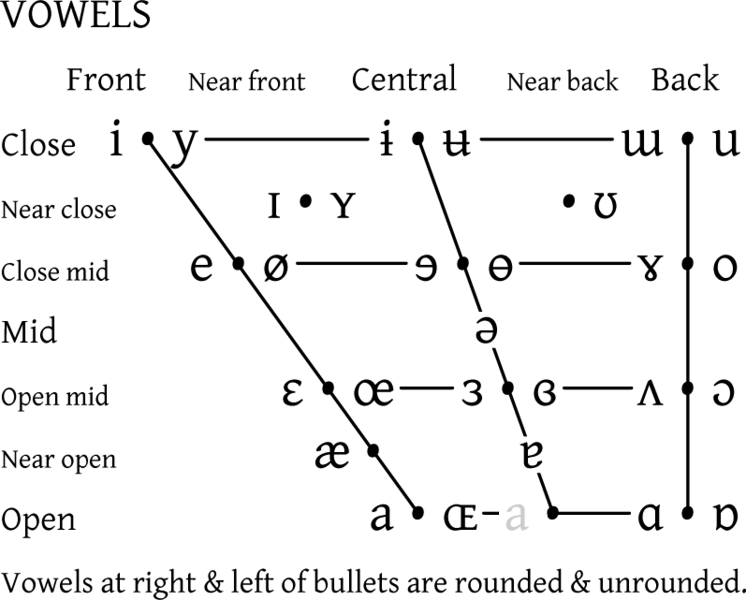
\includegraphics[scale=0.27]{material/04ipavowelwikicommons}
%%		\caption{Vokale}
%		%old picture
%		%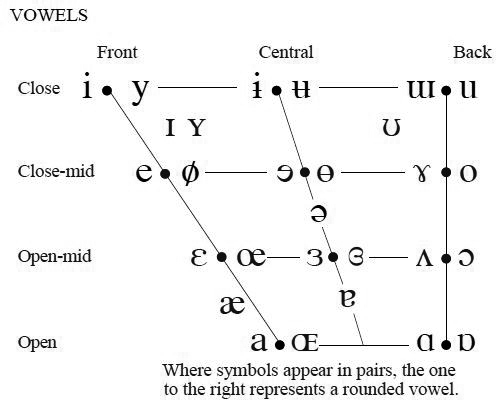
\includegraphics[scale=0.45]{material/04ipavowel}
%		%\caption{Vokale}
%		%\label{Zeichen1}
%	\end{figure}
	
\end{frame}


%%%%%%%%%%%%%%%%%%%%%%%%%%%%%%%%%%%
\begin{frame}
\frametitle{Vokale im Deutschen}

\noindent
\begin{minipage}{.55\textwidth}
	\centerline{
	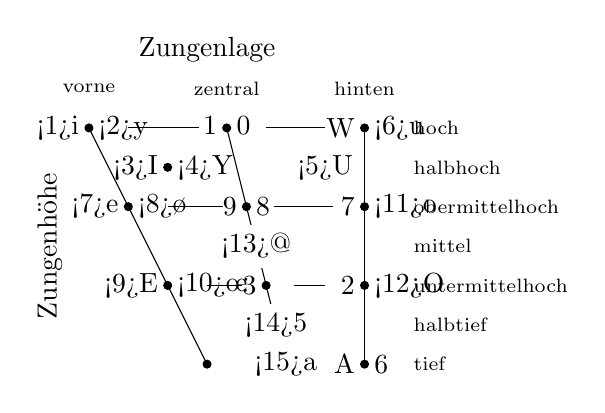
\begin{tikzpicture}
	\draw[fill] (0,0) circle [radius=0.05];
	\draw[fill] (-0.5,1) circle [radius=0.05];
	\draw[fill] (-1,2) circle [radius=0.05];
	\draw[fill] (-1.5,3) circle [radius=0.05];
	\draw[black] (0.5,0)--(0.75,0);
	\draw[black] (1.25,0)--(1.5,0);
	\draw[fill] (2,0) circle [radius=0.05];
	\draw[fill] (2,1) circle [radius=0.05];
	\draw[fill] (2,2) circle [radius=0.05];
	\draw[fill] (2,3) circle [radius=0.05];
	\draw[fill] (0.25,3) circle [radius=0.05];
	\draw[black] (0.25,3)--(1,0);
	\draw[black] (-0.1,3)--(-1,3);
	\draw[black] (0.75,3)--(1.5,3);
	\draw[fill] (0.5,2) circle [radius=0.05];
	\draw[fill] (0.75,1) circle [radius=0.05];
	\node[right] at (0.25,3){\strut \textipa{0}};
	\node[left] at (0.25,3){\strut \textipa{1}};
	\node at (0,4){Zungenlage};
	\node [rotate=90] at (-2,1.5){Zungenhöhe};
	\node at (-1.5,3.5){{\scriptsize vorne}};
	\node at (0.25,3.5){\scriptsize zentral};
	\node at (2,3.5){{\scriptsize hinten}};
	\node[right] at (2.5,3){\scriptsize hoch};
	\node[right] at (2.5,2.5){\scriptsize halbhoch};
	\node[right] at (2.5,2){\scriptsize obermittelhoch};
	\node[right] at (2.5,1.5){\scriptsize mittel};
	\node[right] at (2.5,1){\scriptsize untermittelhoch};
	\node[right] at (2.5,0.5){\scriptsize halbtief};
	\node[right] at (2.5,0){\scriptsize tief};
	\node[left] at (2,3){\textipa{W}};
	\node[right] at (2,3){\alertred{\alertgreen<6>{\textipa{u}}}};
	\node at (1.5,2.5){\alertred{\alertgreen<5>{\textipa{U}}}};
	\node[left] at (2,2){\textipa{7}};
	\node[right] at (2,2){\alertred{\alertgreen<11>{\textipa{o}}}};
	\node[left] at (2,1){\textipa{2}};
	\node[right] at (2,1){\alertred{\alertgreen<12>{\textipa{O}}}};
	\node[right] at (2,0){\textipa{6}};
	\node[left] at (2,0){\textipa{A}};
	\draw[black] (2,0)--(2,3);
	\node[left] at (0.5,2){\textipa{9}};
	\node[right] at (0.5,2){\textipa{8}};
	\node[rectangle,fill=white] at (0.625,1.5){\alertred{\alertgreen<13>{\textipa{@}}}};
	\node[left] at (0.75,1){\textipa{3}};
	\node[right] at (0.75,1){\textipa{\textcloserevepsilon}};
	\node[rectangle,fill=white] at (0.875,0.5){\alertred{\alertgreen<14>{\textipa{5}}}};
	\node[rectangle,fill=white] at (1,0){\alertred{\alertgreen<15>{\textipa{a}}}};
	\node[right] at (-1.5,3){\alertred{\alertgreen<2>{\strut \textipa{y}}}};
	\node[left] at (-1.5,3){\alertred{\alertgreen<1>{\strut \textipa{i}}}};
	\node[left] at (-0.5,2.5){\alertred{\alertgreen<3>{\textipa{I}}}};
	\node[right] at (-0.5,2.5){\alertred{\alertgreen<4>{\textipa{Y}}}};
	\draw[fill] (-0.5,2.5) circle [radius=0.05];
	\node[right] at (-1,2){\alertred{\alertgreen<8>{\textipa{\o}}}};
	\node[left] at (-1,2){\alertred{\alertgreen<7>{\textipa{e}}}};
	\node[right] at (-0.5,1){\alertred{\alertgreen<10>{\textipa{\oe}}}};
	\node[left] at (-0.5,1){\alertred{\alertgreen<9>{\textipa{E}}}};
	\node[right] at (0,0){\textipa{\textscoelig }};
	\draw[black] (0,0)--(-1.5,3);
	\draw[black] (-0.5,2)--(0.2,2);
	\draw[black] (0.85,2)--(1.6,2);
	\draw[black] (0,1)--(0.45,1);
	\draw[black] (1.1,1)--(1.5,1);
	\end{tikzpicture}
}

\medskip

Deutsche Vokale sind \alt<handout>{unterstrichen.}{rot.}
\end{minipage}
\hfill
\begin{minipage}{.42\textwidth}
	\begin{itemize}
	\item Liege [\textipa{li:g@}]\pause,  Lüge [\textipa{ly:g@}]\pause
	\item Kiste [\textipa{kIst@}]\pause,  Küste [\textipa{kYst@}]\pause
	\item muss [\textipa{mUs}]\pause,   Mus   [\textipa{mu:s}]\pause
	\item Wege  [\textipa{ve:g@}]\pause,  wöge [\textipa{vø:g@}]\pause
	\item helle [\textipa{hEl@}]\pause,   Hölle [\textipa{hœl@}]\pause
	\item Ofen  [\textipa{o:f@n}]\pause,  offen [\textipa{Of@n}]\pause
	\item geben [\textipa{ge:b@n}]\pause, Lehrer [\textipa{le:K5}]\pause
	\item Lab   [\textipa{la:p}]
	\end{itemize}
\end{minipage}
\end{frame}


%%%%%%%%%%%%%%%%%%%%%%%%%%%%%%%%%%%
\begin{frame}
\frametitle{Suprasegmentalia}

\begin{tabular}{l|p{6cm}|p{3cm}}
\textbf{Zeichen} &	\textbf{Erklärung} & \textbf{Beispiel} \\
\hline
\alertred{\textipa{\textprimstress}} & Hauptbetonung &[\textipa{Pa.po.\textprimstress te:.k@}]\\

\alertred{\textipa{\textsecstress}} & Nebenbetonung & [\textipa{\textprimstress ba:n.ho:fs.\textsecstress plE:.n@}]\\

\alertred{\textipa{:}} & lang & [\textipa{ba:n}] (vs. [\textipa{ban}])\\

\textipa{;} & halblang & \\

\textipa{\u{}} \textipa{\alertred{\textsubarch{ }}} & extra-kurz/unsilbischer Vokal & [\textipa{stu:d\textsubarch{i}@}], [\textipa{stu:d\u{i}@}]\\

\textipa{\textvertline} & untergeordnete Intonationsgruppe &\\

\textipa{\textdoublevertline} &	übergeordnete Intonationsgruppe & \\

\alertred{\textipa{.}} & Silbengrenze & [\textipa{\textprimstress zIl.bEn.\textsecstress gKEn.\t{ts}@}]\\

\alertred{\textipa{\t{}}} & Doppelartikulation & [\textipa{P\t{aU}to}],  [\textipa{nE\t{ts}}] \\

\alertred{\textipa{\.}} & Silbengelenkmarker & \textipa{[kO\.m@]}\\

\alertred{\textipa{\textsyllabic{ }}} & silbische Konsonanten & \textipa{[kUm.p\textsyllabic{l}]}\\
\end{tabular}

\medskip

Die rot markierten Zeichen werden Sie häufiger in diesem und in zukünftigen Seminaren sehen.

\end{frame}


%%%%%%%%%%%%%%%%%%%%%%%%%%%%%%%%%%%
%%%%%%%%%%%%%%%%%%%%%%%%%%%%%%%%%%%
\subsection{Artikulatorische Phonetik}

%% MyP: Contents
\iftoggle{sectoc}{
	\frame{
		%\begin{multicols}{2}
		\frametitle{~}
		\tableofcontents[currentsubsection,subsubsectionstyle=hide]
		%\end{multicols}
	}
}

%% StM: Contents
\iftoggle{gliederung}{
\outline{

\begin{itemize}

\item Einführung
\item Bereiche der Phonetik
\item  Methodik
\item  Probleme der Phonetik
\item  IPA-Alphabet
\item \blaubf{Artikulatorische Phonetik}
\begin{itemize}
\item Konsonanten
\item Konsonantenklassiffikation
\item Vokale
  \item Vokalklassiffikation
\item Vokalviereck
\item Monophthong, Diphthong, Triphthong
    \end{itemize}
\item Übungen
  
  \end{itemize}
	}
}


%%%%%%%%%%%%%%%%%%%%%%%%%%%%%%%%%%%
\begin{frame}{Artikulatorische Phonetik: Initiator, Generator, Modifikator}

Mehrere Körperteile sind für Erzeugung von Schall nötig:
		
\begin{itemize}
	\item \textbf{Initiator}:\\
	die Lunge \ras (Atmung) erzeugt Luftstrom
	
	\item \textbf{Generator}:\\
	der Kehlkopf (Larynx) mit den Stimmbändern \ras\\
	Luftstrom wird in Schwingung versetzt (Phonation)

	\item \textbf{Frequenz}: Häufigkeit, mit der die Stimmlippen schwingen\\
	\medskip
	Frequenz bestimmt die Tonhöhe:
	
	\begin{itemize}
		\item bei Frauen ung. 230 Hz
		\item bei Männern 120 Hz 
		\item bei Säuglingen 400 Hz
	\end{itemize}

\end{itemize}

\textbf{VIDEO:} \href{run:material/04TransNasalEndoscopy.mp4}{Trans-Nasal Endoscopy}


\end{frame}


%%%%%%%%%%%%%%%%%%%%%%%%%%%%%%%%%%%
\begin{frame}{Artikulatorische Phonetik: Initiator, Generator, Modifikator}

Mehrere Körperteile sind für Erzeugung von Schall nötig:

\begin{itemize}
	\item \textbf{Modifikator}: Rachen-, Mund- und Nasenraum mit den verschiedenen Sprechwerkzeugen (Zunge, Lippen, weicher Gaumen)

\medskip
	
	Unterschiedliche Stellung der Artikulationsorgane verändert den Rohschall des Kehlkopfs zu den wohlunterschiedenen Lauten (Artikulation im engeren Sinne).
\end{itemize}
	
\end{frame}


%%%%%%%%%%%%%%%%%%%%%%%%%%%%%%%%%%%
%%%%%%%%%%%%%%%%%%%%%%%%%%%%%%%%%%%
\subsubsection{Konsonanten}
%%% MyP: Contents
%\iftoggle{sectoc}{
%	\frame{
%		%\begin{multicols}{2}
%		\frametitle{~}
%		\tableofcontents[currentsubsubsection]
%		%\end{multicols}
%	}
%}
%%%%%%%%%%%%%%%%%%%%%%%%%%%%%%%%%%%
\begin{frame}{Konsonanten}

	\begin{itemize}
		\item auch genannt: Mitlaute
		
		\item Die Artikulationsorgane bilden eine \textbf{geräuschverursachende Enge} oder einen \textbf{Verschluss} im Ansatzrohr, \dash die Luft wird oberhalb der Stimmritze (Glottis) zwischen den Stimmbändern behindert.
	\end{itemize}
	
\end{frame}


%%%%%%%%%%%%%%%%%%%%%%%%%%%%%%%%%%%
\begin{frame}
\frametitle{Sagittalschnitt}

\begin{minipage}{0.48\textwidth}
	\begin{figure}
	\centering
	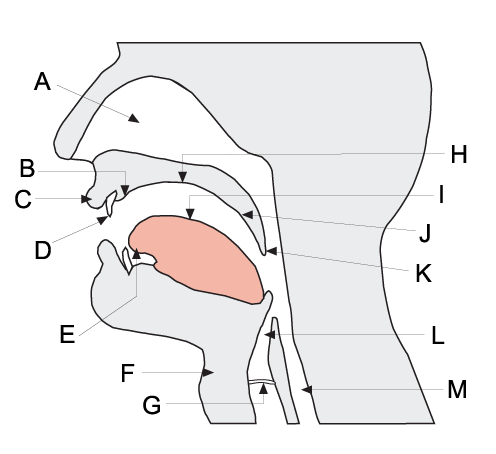
\includegraphics[scale=0.32]{material/04phonoatonomy}
	\caption{Sagittalschnitt}
	\end{figure}
\end{minipage}\hfill
\begin{minipage}{0.4\textwidth}
	A -- Nasenraum\\
	B -- Zahndamm \emph{Alveolen}\\
	C -- (Ober)Lippe \\
	D -- (obere) Zähne\\
	E -- Zungenspitze \emph{Apex}\\
	F -- Kehlkopf \emph{Larynx}\\
	G -- Stimmlippen \emph{Glottis}\\
	H -- harter Gaumen \emph{Palatum}\\
	I -- Zungenrücken \emph{Dorsum}\\
	J -- Gaumensegel \emph{Velum}\\
	K -- Zäpfchen \emph{Uvula}\\
	L -- Luftröhre\\ 
	M -- Speiseröhre
\end{minipage}
	
%	\begin{figure}[H] %%altes Bild%%
%		\centering
%		
%		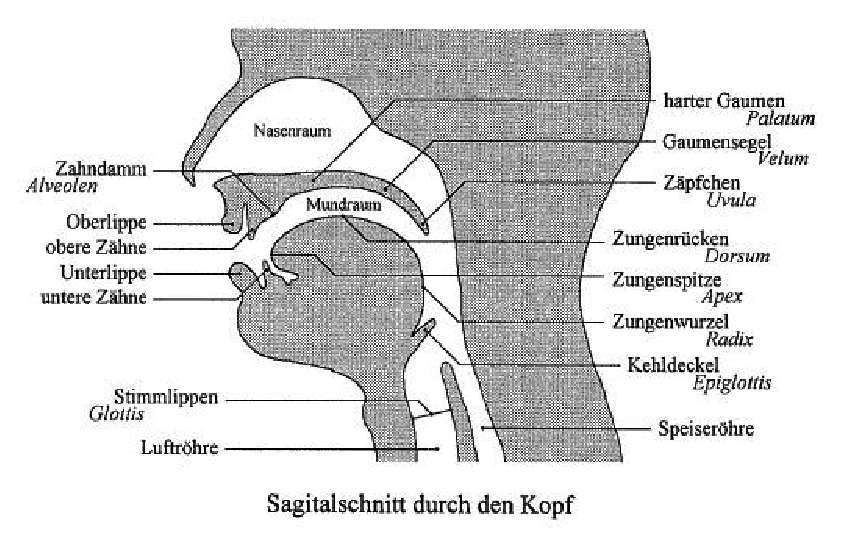
\includegraphics[scale=0.65]{material/04sagitalschnittaltmann}
%		\caption{Sagitalschnitt \citep{Altmann&Co07a}}
%		%\label{Zeichen1}
%	\end{figure}
	
\end{frame}


%%%%%%%%%%%%%%%%%%%%%%%%%%%%%%%%%%%
%%%%%%%%%%%%%%%%%%%%%%%%%%%%%%%%%%%
\subsubsection{Konsonantenklassifikation}
%%% MyP: Contents
%\iftoggle{sectoc}{
%	\frame{
%		%\begin{multicols}{2}
%		\frametitle{~}
%		\tableofcontents[currentsubsubsection]
%		%\end{multicols}
%	}
%}
%%%%%%%%%%%%%%%%%%%%%%%%%%%%%%%%%%%
\begin{frame}{Konsonantenklassifikation: Stimmbeteiligung}

	\begin{itemize}
		\item \textbf{Stimmbeteiligung} (Stimmhaftigkeit): Schwingungszustand der Stimmbänder
		
		\begin{itemize}
			
			\item \textbf{stimmlos} \ras weit auseinander stehende Stimmbänder
			
			\item \textbf{stimmhaft} \ras eng beieinander stehende Stimmbänder
			
			\ea \textipa{[ p ]} vs. \textipa{[ b ]}
			\z

			
			\item \textbf{Aspiration} (Behauchung):\par
				Glottis während der Verschlussphase ist weit gespreizt und schwingt mit.

			\ea \textipa{[ \super h ]}
			\z

                        \textbf{VIDEO:} \href{run:material/02-aspiration.mp4}{Aspiration}
		\end{itemize}

	\end{itemize}
	
\end{frame}


%%%%%%%%%%%%%%%%%%%%%%%%%%%%%%%%%%
\begin{frame}
\frametitle{Übung}
Welche der folgenden Laute sind stimmhaft und welche stimmlos?

\ea \label{ex:02sth}
\textipa{[ d, z, f, v, g, k, P ]}
\z

\end{frame}


%%%%%%%%%%%%%%%%%%%%%%%%%%%%%%%%%%
\iftoggle{ue-loesung}{
	%%%%%%%%%%%%%%%%%%%%%%%%%%%%%%%%%%
%% UE 2 - 02 Phonetik
%%%%%%%%%%%%%%%%%%%%%%%%%%%%%%%%%%

\begin{frame}
\frametitle{Übung -- Lösung}

Welche der folgenden Laute sind stimmhaft und welche stimmlos?

\begin{exe}
\exr{ex:02sth} \textipa{[ d, z, f, v, g, k, P ]}
\end{exe}


\begin{multicols}{2}
	\begin{itemize}
		\item \textbf{stimmhaft:} \alertgreen{\textipa{[ d, z, v, g ]}}
		
		\ea \alertgreen{\textipa{[ d ]}: \ab{Dampf}}
		
		\ex \alertgreen{\textipa{[ z ]}: \ab{Sinn}}
		
		\ex \alertgreen{\textipa{[ v ]}: \ab{Wald}}
		
		\ex \alertgreen{\textipa{[ g ]}: \ab{ganz}}
		
		\z 
	\end{itemize}
	
	\columnbreak \pause
	
	\begin{itemize}
		\item \textbf{stimmlos:} \alertgreen{\textipa{[ f, k, P ]}}
		
		\ea \alertgreen{\textipa{[ f ]}: \ab{Fass}}
		
		\ex \alertgreen{\textipa{[ k ]}: \ab{kalt}}
		
		\ex \alertgreen{\textipa{[ P ]}: \ab{vereisen}}
		
		\z
	\end{itemize}
	
\end{multicols}

\end{frame}


}

%%%%%%%%%%%%%%%%%%%%%%%%%%%%%%%%%%%%
\begin{frame}
\frametitle{Konsonantenklassifikation: Stellung des Gaumensegels}

	\begin{itemize}
		\item \textbf{Stellung des Gaumensegels} (des weichen Gaumens):
		
		\begin{itemize}
			
			\item Nasale Laute (\zB \textipa{ [ m, n ]}) \ras Senkung des weichen Gaumens (Velum)
			
			\item Orale Laute (\zB \textipa{ [ f, a ]}) \ras bei gehobenem Velum
		\end{itemize}
		
		
		\item[] \textbf{LINK:} \href{http://smu-facweb.smu.ca/~s0949176/sammy/}{interaktiver Sagittalschnitt}
	\end{itemize}
	
\end{frame}


%%%%%%%%%%%%%%%%%%%%%%%%%%%%%%%%%%%
\begin{frame}
\frametitle{Konsonantenklassifikation: Artikulationsort (I)}

	\begin{itemize}
	\item \textbf{Artikulationsort} im Vokaltrakt: Ort, an dem die Luft behindert wird
          Unterscheidung nach nicht-beweglichen und beweglichen Artikulatoren

\medskip
		
		\item \textbf{Nicht-bewegliche} Artikulatoren (passiver Artikulator, Artikulationsort im engeren Sinne):
			
		\begin{itemize}
			\item die oberen Zähne \ras \textbf{dental}
			
			\item die Alveolen (Knochendamm hinter den oberen Zähnen) \ras \textbf{alveolar}
			
			\item der harte Gaumen (Palatum) \ras \textbf{palatal}
		\end{itemize}
		
	\end{itemize}
	
\end{frame}


%%%%%%%%%%%%%%%%%%%%%%%%%%%%%%%%%%%
\begin{frame}
\frametitle{Konsonantenklassifikation: Artikulationsort (II)}

\begin{itemize}
	\item \textbf{Bewegliche} Artikulatoren (aktiver Artikulator, Artikulationsorgan):
			
	\begin{itemize}
		
		\item weicher Gaumen (Velum) \ras \textbf{velar}
		
		\item das Zäpfchen (Uvula) \ras \textbf{uvular}
		
		\item Lippen \ras \textbf{labial}
		
		\item Unterkiefer
		
		\item Zunge
	\end{itemize}

\end{itemize}

\end{frame}


%%%%%%%%%%%%%%%%%%%%%%%%%%%%%%%%%%%
\begin{frame}
\frametitle{Konsonantenklassifikation: Artikulationsort (III)}

		\begin{itemize}
			\item Bei der Artikulation mit der \textbf{Zunge} bildet man Untergruppen nach dem \textbf{beteiligten Zungenteil}:
			
			\begin{itemize}
				\item \textbf{koronal}: mit dem vorderen Teil der Zunge
	
				\begin{itemize}
					\item \textbf{apikal}: mit der Zungenspitze
					
					\item \textbf{laminal}: mit dem Zungenblatt (mittlerer Teil der Zunge)				
				\end{itemize}
	
				\ea \textipa{[ t, d, l, n, s, z, S, Z ]}
				\z

\pause

				\item \textbf{dorsal}: mit dem hinteren Teil der Zunge

				\ea \textipa{[ \c{c}, j, g, k, x, N, \textscr, K ]}
				\z

			\end{itemize}

					
		\item[] \textbf{LINK:} \href{http://smu-facweb.smu.ca/~s0949176/sammy/}{Interaktiver Sagittalschnitt}

		\end{itemize}
		
\end{frame}


%%%%%%%%%%%%%%%%%%%%%%%%%%%%%%%%%%%
\begin{frame}
\frametitle{Konsonantenklassifikation: Artikulationsart}

	\begin{block}{Artikulationsart}
	(auch Artikulationsmodus)\\
	Art der Behinderung des Luftstroms durch die Artikulationsorgane
	\end{block}	

\end{frame}


%%%%%%%%%%%%%%%%%%%%%%%%%%%%%%%%%%%
\begin{frame}
\frametitle{Artikulationsart: Plosive}

\begin{itemize}
			\item \textbf{Plosive} (Verschlusslaute, Explosivlaute, stops): totaler oraler Verschluss mit anschließender plötzlicher Lösung des Verschlusses\\
				Das Velum bleibt dabei in angehobener Position,\par
				so dass die Luft durch den Mundraum strömt.

			\ea \textipa{[ p, b, t, d, k, g, P ]}
			\z
			
			Der \textbf{Glottalverschluss} (Knacklaut) \textipa{[ P ]} entsteht durch plötzliches Öffnen der Stimmritze und kommt im Deutschen vor anlautendem Vokal eines Wortes und vor anlautendem Vokal in einer betonten Silbe vor.
		
	\end{itemize}
	
\end{frame}


%%%%%%%%%%%%%%%%%%%%%%%%%%%%%%%%%%%
\begin{frame}
\frametitle{Artikulationsart: Frikative}

		\begin{itemize}
			\item \textbf{Frikative} (Reibelaute, Spiranten): Verengung zweier Sprechorgane,\\
                          Luftstrom strömt durch die Verengung, es entsteht ein Reibegeräusch.

			\ea \textipa{[ f, v, s, z, S, Z, \c{c}, x, h, K ]}
			\z

\pause 
			
			\begin{itemize}
				\item \textbf{Sibilanten} (Zischlaut):\par
					Unterklasse der Frikative mit intensivem, hochfrequentem Geräuschanteil.

				\ea \textipa{[ s, z, S ]}
				\z

		\end{itemize}
		
	\end{itemize}
	
\end{frame}


%%%%%%%%%%%%%%%%%%%%%%%%%%%%%%%%%%%
\begin{frame}
%\frametitle{Konsonantenklassifikation}
\frametitle{Artikulationsart: Affrikaten}

		\begin{itemize}
			\item \textbf{Affrikaten}: Plosive, die in Frikative übergehen, wobei die Verschlussphase und die Frikativphase dieselbe (oder annähernd dieselbe) Artikulationsstelle haben; d.\,h. sie sind \textbf{homorgan}.

			\ea \textipa{[ \texttoptiebar{pf}, \texttoptiebar{ts}, \texttoptiebar{tS}, \texttoptiebar{dZ} ]} %\textipa{ \t{aUI}}
			\z

			\begin{itemize}
				\item Per Definition gehören der plosive und der frikative Laut einer Affrikaten \textbf{zum selben Morphem} (die kleinste bedeutungstragende Einheit). Daraus ergibt sich:

				\ea \textipa{[ \t{ts} ]} in \ab{Blitz} \ras Affrikate
				\z
				
				\ea \textipa{[ ts ]} in \ab{Monats} \ras keine Affrikate
				\z

			\end{itemize}
		
		
		\item Plosive, Frikative und Affrikaten \ras \textbf{Obstruenten}
	\end{itemize}
	
\end{frame}


%%%%%%%%%%%%%%%%%%%%%%%%%%%%%%%%%%%
\begin{frame}
\frametitle{Artikulationsart: Vibranten}

		\begin{itemize}
			\item \textbf{Vibranten} (trills): schnelle Folge oraler Verschlüsse
			\begin{itemize}
				
				\item Artikulationsstellen für Vibranten sehr eingeschränkt: nur bilabial, alveolar oder uvular
				
				\item Der alveolare Vibrant \textipa{[ r ]} (das sog. Zungenspitzen-R) kommt in vielen süddeutschen Varietäten vor.
				
				\item Der uvulare Vibrant \textipa{[ \textscr\ ]} (das gerollte Zäpfchen-R) ist eine häufige Realisierung des Deutschen \ab{r}.
			\end{itemize}
			 
	\end{itemize}
	
\end{frame}


%%%%%%%%%%%%%%%%%%%%%%%%%%%%%%%%%%%
\begin{frame}
\frametitle{Artikulationsart: Approximanten}

		\begin{itemize}
			\item \textbf{Approximanten} (Öffnungslaute): Enge im Ansatzrohr (wie Frikative)\\
			Bei Approximanten gibt es nicht so eine große Nähe zwischen Artikulator und Artikulationsstelle \ras kein Reibegeräusch
			
			 Zwei Unterklassen:
			
			\begin{itemize}
				
				\item \textbf{Laterale}: Verschluss in der Mundhöhlenmitte, Luft entweicht seitlich [~\textipa{l}~]
				
				\item \textbf{Gleitlaute} (zentral): zentrale Verengung, aber weiter als bei Frikativen [~\textipa{w}~].\\
				(Manchmal wird [~\textipa{j}~] auch zu den Gleitlauten gezählt,\\
                                  da die Verengung weiter als bei anderen Frikativen ist. Dies ist jedoch strittig.)
			\end{itemize}
			
		\end{itemize}	

\end{frame}


%%%%%%%%%%%%%%%%%%%%%%%%%%%%%%%%%%%
\begin{frame}
%\frametitle{Konsonantenklassifikation}
\frametitle{Artikulationsart: Nasale}
		\begin{itemize}
			\item \textbf{Nasale}: totaler oraler Verschluss (wie Plosive).\\
				Luft entweicht durch die Nase durch Senken des Velums.
			 
			 \ea \textipa{[ m, n, N ]}
			 \z
		
		\item Vibranten, Approximanten (Laterale und Gleitlaute), Nasale und Vokale (auch die hier nicht behandelten \gqq{geschlagenen Laute} wie das span. \textipa{[~R~]}) gehören zur Gruppe der \textbf{Sonoranten}, da die Luft ungehindert ausströmen kann. Sonoranten sind \textbf{immer} stimmhaft!
		
		\item Die Klasse der l-Laute und r-Laute werden auch zu den sog. \textbf{Liquiden} zusammengefasst (im Dt. \textipa{[ l, r, \textscr ]})
	\end{itemize}

	
\end{frame}


%%%%%%%%%%%%%%%%%%%%%%%%%%%%%%%%%%%
\begin{frame}
	\frametitle{Konsonantenklassifikation: Zusammenfassung I}
	
\begin{figure}
	\centering
	
\scalebox{.85}{
\begin{forest}
	sm edges
	[Konsonanten
		[\textbf{Obstruenten}\\{[}$-$son{]}
			[Frikative\\{[}$+$kont{]}
				[{[}$+$sth{]} [\textipa{v z Z}, no edge] ]
				[{[}$-$sth{]} [\textipa{f s S \c{c}}, no edge] ]
			]
			[Plosive\\{[}$-$kont{]}
				[{[}$+$sth{]} [\textipa{b d g}, no edge] ]
				[{[}$-$sth{]} [\textipa{p t k}, no edge] ]
			]
		]
		[\textbf{Sonoranten}\\{[}$-$son{]}
			[Liquide\\{[}$-$nas{]}
				[Laterale\\{[}$+$lat{]} [\textipa{l}, no edge] ]
				[Vibranten\\{[}$-$lat{]} [\textipa{r  R K}, no edge] ]
			]
			[Nasale\\{[}$+$nas{]} [\textipa{m n N}, no edge] ]
		]
	]
\end{forest}
}

\end{figure}

Zur Gruppe der \textbf{Sonoranten} zählen alle Konsonanten, bei denen die Luft \textbf{ungehindert} ausströmen kann. Sie sind \textbf{immer stimmhaft}.

Obstruenten können stimmhaft oder auch stimmlos sein.
	
\end{frame}


%%%%%%%%%%%%%%%%%%%%%%%%%%%%%%%%%%%
\begin{frame}
	\frametitle{Konsonantenklassifikation: Zusammenfassung II}

	\begin{itemize}
		\item Für die \textbf{Differenzierung der deutschen Konsonanten} sind hauptsächlich 3 Merkmale wichtig:
		
		\begin{itemize}
			
			\item Stimmbeteiligung
			\item Artikulationsort
			\item Artikulationsart
		\end{itemize}
	\end{itemize}

\textbf{LINK}: \href{http://www.ipachart.com/}{Interactive IPA chart}

\end{frame}


%%%%%%%%%%%%%%%%%%%%%%%%%%%%%%%%%%
\begin{frame}

\frametitle{Übung}

\begin{itemize}
	\item[] Beschreiben Sie die Konsonanten in den folgenden Wörtern und geben Sie die entsprechenden phonetischen Symbole an:
	
	\begin{enumerate}
		\item Busch
		\item malen
		\item Maus
		\item Achtung
		\item Genie
		\item zirpen
		\item wichtig
		\item Wald
	\end{enumerate}
	
\end{itemize}
\end{frame}


%%%%%%%%%%%%%%%%%%%%%%%%%%%%%%%%%%%
\iftoggle{ue-loesung}{
	%%%%%%%%%%%%%%%%%%%%%%%%%%%%%%%%%%
%% UE 3 - 02 Phonetik
%%%%%%%%%%%%%%%%%%%%%%%%%%%%%%%%%%

\begin{frame}
\frametitle{Übung -- Lösung}

\begin{table}
\scalebox{.9}{
	\begin{tabular}{llp{9cm}}
		1. Busch & \alertgreen{\only<2->{[\textipa{bUS}]}} & \only<3->{\textipa{b}: bilabialer, stimmhafter Plosiv; \textipa{S}:~postalveolarer, stimmloser Frikativ} \\
		
		2. malen & \alertgreen{\only<4->{[\textipa{\textprimstress ma:l@n}]}} & \only<5->{\textipa{m}:~bilabialer, stimmhafter Nasal; \textipa{n}:~alveolarer, stimmhafter Nasal; \textipa{l}:~alveolar, stimmhafter Lateral} \\
		
		3. Maus & \alertgreen{\only<6->{[\textipa{m\texttoptiebar{aU}s}]}} & \only<7->{\textipa{m}:~s.\,o.; \textipa{s}:~stimmloser, alveolarer Frikativ} \\
		
		4. Achtung & \alertgreen{\only<8->{[\textipa{\textprimstress PaXtU\ng}]}} & \only<9->{\textipa{P}:~glottaler, stimmloser Plosiv; \textipa{X}:~velarer, stimmloser Frikativ; \textipa{t}:~alveolarer, stimmloser Plosiv; \textipa{\ng}: velarer, stimmhafter Nasal} \\

		5. Genie & \alertgreen{\only<10->{[\textipa{Ze:\textprimstress ni:}]}} & \only<11->{\textipa{Z}: postalveolarer, stimmhafter Frikativ; \textipa{n}:~s.\,o.} \\                
		                                                                                  
		6. zirpen & \alertgreen{\only<12->{[\textipa{\texttoptiebar{ts}IKp@n}]}} & \only<13->{\textipa{\texttoptiebar{ts}}: alveolare, stimmlose Affrikate; \textipa{K}:~uvularer, stimmhafter Frikativ; \textipa{p}:~bilabialer, stimmloser Plosiv; \textipa{n}: s.\,o.} \\

		7. wichtig & \alertgreen{\only<14->{[\textipa{\textprimstress vI\c{c}tI\c{c}}]}} & \only<15->{\textipa{v}: labiodentaler, stimmhafter Frikativ; \textipa{\c{c}}: palataler, stimmloser Frikativ; \textipa{t}: s.\,o.} \\

		8. Wald & \alertgreen{\only<16->{[\textipa{valt}]}} & \only<17->{\textipa{v, l, t}: s.\,o.}
\end{tabular}
}
\end{table}

\end{frame}

}
%%%%%%%%%%%%%%%%%%%%%%%%%%%%%%%%%%%

%%%%%%%%%%%%%%%%%%%%%%%%%%%%%%%%%%
%%%%%%%%%%%%%%%%%%%%%%%%%%%%%%%%%%
\subsubsection{Vokale}

%%% MyP: Contents
%\iftoggle{sectoc}{
%	\frame{
%		%\begin{multicols}{2}
%		\frametitle{~}
%		\tableofcontents[currentsubsubsection]
%		%\end{multicols}
%	}
%}
%%%%%%%%%%%%%%%%%%%%%%%%%%%%%%%%%%%
\begin{frame}{Vokale}

	\begin{itemize}
		\item \textbf{Vokale} (Selbstlaute) sind Laute, bei deren Artikulation die Luft ungehindert durch den Mundraum strömen kann (deswegen gehören sie zu den \textbf{Sonoranten}).
		
		\item Vokale sind \idR immer \textbf{stimmhaft}.
		
		\item Es ist umstritten, ob der sog. Schwa-Laut im Dt. \textipa{[ @ ]} stimmhaft
                  ist.\\
                  Auch im Japanischen soll es stimmlose Vokale geben.
	\end{itemize}
	
\end{frame}


%%%%%%%%%%%%%%%%%%%%%%%%%%%%%%%%%%%
%%%%%%%%%%%%%%%%%%%%%%%%%%%%%%%%%%%
\subsubsection{Vokalklassifikation}
%%% MyP: Contents
%\iftoggle{sectoc}{
%	\frame{
%		%\begin{multicols}{2}
%		\frametitle{~}
%		\tableofcontents[currentsubsubsection]
%		%\end{multicols}
%	}
%}
%%%%%%%%%%%%%%%%%%%%%%%%%%%%%%%%%%%

\begin{frame}{Vokalklassifikation I}

	\begin{itemize}
		\item \textbf{Zungenhöhe} (Vokalhöhe): Grad der Zungenhebung in Richtung Gaumen

		\ea hoch: \textipa{[ i: ]}, mittel: \textipa{[ o: ]}, tief: \textipa{[ a: ]} bzw. geschlossen, halboffen, offen
		\z

\pause 

		\item \textbf{Zungenlage} (Vokaltiefe): angehobener Teil der Zunge

		\ea vorne: \textipa{[ i: ]}, zentral: \textipa{[ a: ]}, hinten: \textipa{[ u: ]}
		\z

\pause 

		\item \textbf{Lippenrundung}: Art der Lippenöffnung

		\ea gerundet: \textipa{[ o: ]}, ungerundet: \textipa{[ i: ]}
		\z

		\bigskip
 

 	\item Lesen Sie folgende Wörter mit \textbf{gerundeten} und mit \textbf{gespreizten} Lippen:
	\ea 
	\ea Bühne, rühmen, Dünen, Stiele, Trieb, Möhre, Herd, Hefe, kennen

\pause 	

	\ex  Biene, Riemen, dienen, Stühle, trüb, Meere, hört, Höfe, können
	\z  
	\z 
 
\end{itemize}

\end{frame}


%%%%%%%%%%%%%%%%%%%%%%%%%%%%%%%%%%%
\begin{frame}
\frametitle{Vokalklassifikation II}

\begin{itemize}
	\item Gespanntheit:

\begin{description}
	\item[\textbf{Definition 1}] \textipa{[ i:, y:, u:, o: ]} mit \textbf{mehr Muskelspannung} als \textipa{[ I, Y, U, O ]} 
	
	(von der experimentellen Phonetik weder bestätigt noch widerlegt)
	
	\item[\textbf{Definition 2}] \textipa{[ i:, y:, u:, o: ]}  mit \textbf{vorverlagerter Zungenwurzel}


\begin{multicols}{2}

\textbf{gespannt:}
	\ea \textipa{[ i: ]}: \ab{Liege}
	
	\ex \textipa{[ y: ]}: \ab{Lüge}
	
	\ex \textipa{[ u: ]}: \ab{Mus}
	
	\ex \textipa{[ o: ]}: \ab{Ofen}
	
	\z 
	
\columnbreak
	
\textbf{ungespannt:}
	\ea \textipa{[ I ]}: \ab{Kiste}
	
	\ex \textipa{[ Y ]}: \ab{Küste}
	
	\ex \textipa{[ U ]}: \ab{muss}
	
	\ex \textipa{[ O ]}: \ab{offen}
	
	\z
	
\end{multicols}

\end{description}
\end{itemize}
			
\end{frame}		

%%%%%%%%%%%%%%%%%%%%%%%%%%%%%%%%%%%			
			
\begin{frame}
\frametitle{Anmerkungen zur Gespanntheit}
		\begin{itemize}	
			\item i.\,d.\,R. alle tiefen Vokale \ras ungespannt (strittig!)
			\item langer tiefer Vokal \textipa{[ a: ]} \ras gespannt(?)
%		\end{itemize}

	      \item im Deutschen: Korrelation der Gespanntheit mit der Länge

		\ea \textipa{[ m i: t @ ]} vs. \textipa{[ m I t @ ]}
		\z

		\item in Lehnwörtern auch kurze gespannte Vokale

		\ea \textipa{[ P i . d e: ]}
		\z
		
	\end{itemize}
	
\end{frame}


%%%%%%%%%%%%%%%%%%%%%%%%%%%%%%%%%%%
\begin{frame}
\frametitle{Vokalklassifikation III}

	\begin{itemize}
	
		
%\vspace{1em}
		
		\item \textbf{Stellung des Gaumensegels}:
		
		\begin{itemize}
			\item oral
			\item nasal
			
			\item Nasalvokale kommen im Dt. nur in Lehnwörtern vor.

			\eal
			\ex \textipa{[ \~a ]} in \ab{Restaur\textbf{ant}}
			\ex \textipa{[ \~E ]} in \ab{T\textbf{eint}}
			\ex \textipa{[ \~o ]} in \ab{Balk\textbf{on}}
			\ex \textipa{[ \~\oe\ ]} in \ab{in Parf\textbf{um}}
			\zl
		
		\end{itemize}
		
	\end{itemize}
	
\end{frame}


%%%%%%%%%%%%%%%%%%%%%%%%%%%%%%%%%%%
\begin{frame}
\frametitle{Vokalklassifikation: Überblick}

	\begin{itemize}
		\item Für die \textbf{Differenzierung der deutschen nativen Vokale} sind hauptsächlich vier Merkmale wichtig:
		
		\begin{itemize}
			
			\item Zungenhöhe
			
			\item Zungenlage
			
			\item Lippenrundung
			
			\item Gespanntheit (bzw. Länge)
		\end{itemize}
		
	\end{itemize}

\textbf{LINK}: \href{http://www.ipachart.com/}{Interactive IPA chart}
	
\end{frame}


%%%%%%%%%%%%%%%%%%%%%%%%%%%%%%%%%%%
%%%%%%%%%%%%%%%%%%%%%%%%%%%%%%%%%%%
\subsubsection{Vokalviereck}
%%% MyP: Contents
%\iftoggle{sectoc}{
%	\frame{
%		%\begin{multicols}{2}
%		\frametitle{~}
%		\tableofcontents[currentsubsubsection]
%		%\end{multicols}
%	}
%}
%%%%%%%%%%%%%%%%%%%%%%%%%%%%%%%%%%%

\begin{frame}{Vokalviereck}

	\begin{itemize}
		\item Vokale wurden 1920 von Daniel Jones im sog. Vokalviereck angeordnet.
		\item Vokalviereck stellt eine stilisierte Version des Vokalraums dar.
	\end{itemize}

\begin{figure}
	\centering
%\scalebox{.8}{	
	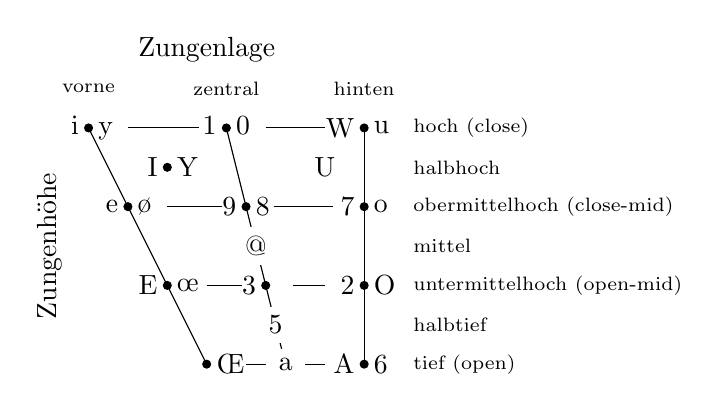
\begin{tikzpicture}
	\draw[fill] (0,0) circle [radius=0.05];
	\draw[fill] (-0.5,1) circle [radius=0.05];
	\draw[fill] (-1,2) circle [radius=0.05];
	\draw[fill] (-1.5,3) circle [radius=0.05];
	\draw[black] (0.5,0)--(0.75,0);
	\draw[black] (1.25,0)--(1.5,0);
	\draw[fill] (2,0) circle [radius=0.05];
	\draw[fill] (2,1) circle [radius=0.05];
	\draw[fill] (2,2) circle [radius=0.05];
	\draw[fill] (2,3) circle [radius=0.05];
	\draw[fill] (0.25,3) circle [radius=0.05];
	\draw[black] (0.25,3)--(1,0);
	\draw[black] (-0.1,3)--(-1,3);
	\draw[black] (0.75,3)--(1.5,3);
	\draw[fill] (0.5,2) circle [radius=0.05];
	\draw[fill] (0.75,1) circle [radius=0.05];
	\node[right] at (0.25,3){\strut \textipa{0}};
	\node[left] at (0.25,3){\strut \textipa{1}};
	\node at (0,4){Zungenlage};
	\node [rotate=90] at (-2,1.5){Zungenhöhe};
	\node at (-1.5,3.5){{\scriptsize vorne}};
	\node at (0.25,3.5){\scriptsize zentral};
	\node at (2,3.5){{\scriptsize hinten}};
	\node[right] at (2.5,3){\scriptsize hoch (close)};
	\node[right] at (2.5,2.5){\scriptsize halbhoch};
	\node[right] at (2.5,2){\scriptsize obermittelhoch (close-mid)};
	\node[right] at (2.5,1.5){\scriptsize mittel};
	\node[right] at (2.5,1){\scriptsize untermittelhoch (open-mid)};
	\node[right] at (2.5,0.5){\scriptsize halbtief};
	\node[right] at (2.5,0){\scriptsize tief (open)};
	\node[left] at (2,3){\textipa{W}};
	\node[right] at (2,3){\textipa{u}};
	\node at (1.5,2.5){\textipa{U}};
	\node[left] at (2,2){\textipa{7}};
	\node[right] at (2,2){\textipa{o}};
	\node[left] at (2,1){\textipa{2}};
	\node[right] at (2,1){\textipa{O}};
	\node[right] at (2,0){\textipa{6}};
	\node[left] at (2,0){\textipa{A}};
	\draw[black] (2,0)--(2,3);
	\node[left] at (0.5,2){\textipa{9}};
	\node[right] at (0.5,2){\textipa{8}};
	\node[rectangle,fill=white] at (0.625,1.5){\textipa{@}};
	\node[left] at (0.75,1){\textipa{3}};
	\node[right] at (0.75,1){\textipa{\textcloserevepsilon}};
	\node[rectangle,fill=white] at (0.875,0.5){\textipa{5}};
	\node[rectangle,fill=white] at (1,0){\textipa{a}};
	\node[right] at (-1.5,3){\strut \textipa{y}};
	\node[left] at (-1.5,3){\strut \textipa{i}};
	\node[left] at (-0.5,2.5){\textipa{I}};
	\node[right] at (-0.5,2.5){\textipa{Y}};
	\draw[fill] (-0.5,2.5) circle [radius=0.05];
	\node[right] at (-1,2){\textipa{\o}};
	\node[left] at (-1,2){\textipa{e}};
	\node[right] at (-0.5,1){\textipa{\oe}};
	\node[left] at (-0.5,1){\textipa{E}};
	\node[right] at (0,0){\textipa{\OE}};
	\draw[black] (0,0)--(-1.5,3);
	\draw[black] (-0.5,2)--(0.2,2);
	\draw[black] (0.85,2)--(1.6,2);
	\draw[black] (0,1)--(0.45,1);
	\draw[black] (1.1,1)--(1.5,1);
	\end{tikzpicture}
%}
	\caption{Vokalviereck}
\end{figure}	
	
\end{frame}


%%%%%%%%%%%%%%%%%%%%%%%%%%%%%%%%%%%
%%%%%%%%%%%%%%%%%%%%%%%%%%%%%%%%%%%
\subsubsection{Monophthong, Diphthong, Triphthong}
%%% MyP: Contents
%\iftoggle{sectoc}{
%	\frame{
%		%\begin{multicols}{2}
%		\frametitle{~}
%		\tableofcontents[currentsubsubsection]
%		%\end{multicols}
%	}
%}
%%%%%%%%%%%%%%%%%%%%%%%%%%%%%%%%%%%

\begin{frame}{Monophthong, Diphthong, Triphthong}

\begin{itemize}
	\item \textbf{Monophthong}

	\begin{itemize}		
		\item einzelner (langer oder kurzer) Vokal
		
	\end{itemize}
	
	\item \textbf{Diphthong} (Zwielaut, Doppellaut)
	
	\begin{itemize}		
		\item Abfolge von zwei Vokalen
		
		\item Beide Einheiten haben zusammen die Dauer eines einzelnen langen Vokals.
		
		\item Beide Vokale gehören zur selben Silbe (im Silbenkern).
		
		\item Zunge gleitet bei der Artikulation von einer Stellung in eine andere.
		
		\item Laut ändert kontinuierlich seine Qualität.
	\end{itemize}
	
\end{itemize}	

\end{frame}


%%%%%%%%%%%%%%%%%%%%%%%%%%%%%%%%%%%
\begin{frame}
\frametitle{Unterklassen der Diphthonge: fallend}
		
		\begin{itemize}
			
			\item auch \emph{schließende Diphthonge} genannt
			\item \gqq{echte}, native deutsche Diphthonge

			\ea \textipa{[~\texttoptiebar{aI}~,~\texttoptiebar{aU}~,~\texttoptiebar{OI}~]} oder \textipa{[ a\textsubarch{I}, a{\textsubarch{U}}, O\textsubarch{I} ]}
			\z

			\item Erster Bestandteil ist prominenter: Prominenz fällt.\par
				(Wäre Prominenz gleich, bekäme man zwei Silben.)
				
			\end{itemize}
	
\end{frame}
%%%%%%%%%%%%%%%%%%%%%%%%%%%%%%%%%%%
\begin{frame}
\frametitle{Unterklassen der Diphthonge: steigend}		

		\begin{itemize}	
			\item auch \emph{öffnende Diphthonge} genannt

			\ea im Bayrischen: \textipa{[ \t{ɪa}, \t{ʊa} ]} oder \textipa{[ \textsubarch{I}a, {\textsubarch{U}}a ]} (in \ab{liap} und \ab{guat})
			\z
			
			\ea in Fremdwörtern: \ab{Span\textbf{ie}n}, \ab{Rit\textbf{ua}l}, \ab{Stud\textbf{iu}m}, \ab{Ling\textbf{ui}stik}
			\z
			
			\item fallend vs. steigend \ras akustisch-auditive Perspektive
			\item schließend vs. öffnend \ras artikulatorische Perspektive
		\end{itemize}
		
\end{frame}


%%%%%%%%%%%%%%%%%%%%%%%%%%%%%%%%%%%
\begin{frame}
\frametitle{Unterklassen der Diphthonge: zentralisierend}

	\begin{itemize}
		\item \textbf{zentralisierende} Diphthonge (durch R-Vokalisierung \ras keine Phoneme)

		\ea 
		\begin{itemize}
			\item \textipa{\texttoptiebar{i5}} \ras hier
			\item \textipa{\texttoptiebar{ɪ5}} \ras Birke
			\item \textipa{\texttoptiebar{e5}} \ras mehr
			\item \textipa{\texttoptiebar{u5}} \ras stur
			\item \textipa{\texttoptiebar{y5}} \ras für
			\item \textipa{\texttoptiebar{ʏ5}} \ras Türme
			\item \textipa{\texttoptiebar{ø5}} \ras Stör
			\item \textipa{\texttoptiebar{ʊ5}} \ras Dortmund
			\item \textipa{\texttoptiebar{O5}} \ras Ohr
		\end{itemize}
		\z
		
	\end{itemize}

\end{frame}


%%%%%%%%%%%%%%%%%%%%%%%%%%%%%%%%%%%
\begin{frame}
\frametitle{Triphthong (Dreilaut)}
	
\begin{itemize}
	\item Abfolge von drei Vokalen im Silbenkern (umstritten)
	\item Anzahl der Silben unsicher

\pause 
			
	\ea Steu-er \vs Steuer
	\ex Bau-er \vs Bauer
	\z

\pause
			
	\item \textbf{linear steigende}
	\item \textbf{linear fallende}
	\item mit \textbf{Umkehrpunkt}

	\ea {[}\textipa{\t{aI}5}]: \ab{Eier}
	\ex {[}\textipa{\texttoptiebar{O}I5}]: \ab{Steuer}
	\ex {[}\textipa{\t{aU}5}]: \ab{Bauer}
	\z	
	
\end{itemize}

\end{frame}

	
%%%%%%%%%%%%%%%%%%%%%%%%%%%%%%%%%%%
%%%%%%%%%%%%%%%%%%%%%%%%%%%%%%%%%%%
\subsection{Übungen}

%% MyP: Contents
\iftoggle{sectoc}{
	\frame{
		%\begin{multicols}{2}
		\frametitle{~}
		\tableofcontents[currentsubsection,subsubsectionstyle=hide]
		%\end{multicols}
	}
}

%% StM: Contents
\iftoggle{gliederung}{
 \outline{

 \begin{itemize}

 \item Einführung
 \item Bereiche der Phonetik
 \item Methodik
 \item Probleme der Phonetik
 \item IPA-Alphabet
 \item Artikulatorische Phonetik
 %% Konsonanten
 %% Konsonantenklassifikation
 %% Vokale
 %% Vokalklassifikation
 %% Vokalviereck
 %% Monophthong, Diphthong, Triphthong
 \item \blaubf{Übungen}
  
   \end{itemize}
 }
}


%%%%%%%%%%%%%%%%%%%%%%%%%%%%%%%%%%%
\begin{frame}
\frametitle{Übungen}

\begin{itemize}
	\item Bilden die folgenden Vokalabfolgen Diphthonge?
	\item[] Zeit, naiv, Haus
\end{itemize}

\end{frame}


%%%%%%%%%%%%%%%%%%%%%%%%%%%%%%%%%
\iftoggle{ue-loesung}{
	%%%%%%%%%%%%%%%%%%%%%%%%%%%%%%%%%%
%% UE 4 - 02 Phonetik
%%%%%%%%%%%%%%%%%%%%%%%%%%%%%%%%%%

\begin{frame}
\frametitle{Übungen -- Lösung}

\begin{itemize}
	\item Bilden die folgenden Vokalabfolgen Diphthonge?
	\item[] Zeit, naiv, Haus
	
	\item \alertgreen{Ja: \textipa{[\texttoptiebar{ts}\texttoptiebar{aI}t]} , \textipa{[h\texttoptiebar{aU}s]}}
	\item \alertgreen{Nein: \textipa{[na.Pi:f]}}
\end{itemize}

\end{frame}
}
%%%%%%%%%%%%%%%%%%%%%%%%%%%%%%%%%

\begin{frame}
\frametitle{Übungen: Transkription}

\begin{itemize}
	
	\item Transkribieren Sie die folgenden Wörter nach einer standarddeutschen Aussprache:
	
		\begin{enumerate}
			\item Bergsteiger
			\item Quotennote
			\item vielfaches
			\item Päckchenannahme
			\item beenden
			\item verreisen
			\item vereisen
			\item Einzahlung
			\item gehen
			\item Gästebad
		\end{enumerate} 

\end{itemize}

\end{frame}


%%%%%%%%%%%%%%%%%%%%%%%%%%%%%%
\iftoggle{ue-loesung}{
	%%%%%%%%%%%%%%%%%%%%%%%%%%%%%%%%%%
%% UE 5 - 02 Phonetik
%%%%%%%%%%%%%%%%%%%%%%%%%%%%%%%%%%

\begin{frame}
\frametitle{Lösung: Transkription}

\begin{itemize}

\item Transkribieren Sie die folgenden Wörter nach einer standarddeutschen Aussprache:

%\begin{columns}
%	\column{.40\textwidth}
	\begin{enumerate}

\settowidth\jamwidth{XXXXXXXXXXXXXXXXXXXXXXXXXXXXXXXXXXXXXX}

		\item  Bergsteiger
		\loesung{1}{\textipa{[bE͡5k.St\t{aI}.g5]}}
		
		\item  Quotennote
		\loesung{2}{\textipa{[kvo:.t@n.no:.t@]}}
		
		\item  vielfaches
		\loesung{3}{\textipa{[fi:l.fa\.x@s]}}
		
		\item  Päckchenannahme
		\loesung{4}{\textipa{[pEk.\c{c}@n.Pan.na:.m@]}}
		
		\item  beenden
		\loesung{5}{\textipa{[b@.PEn.d@n]}}
		
		\item  verreisen
		\loesung{6}{\textipa{[fE͡5.\textscr \t{aI}.z@n]}}
		
		\item  vereisen
		\loesung{7}{\textipa{[fE͡5.P\t{aI}.z@n]}}
		
		\item  Einzahlung
		\loesung{8}{\textipa{[P\t{aI}n.\t{ts}a:.lUN]}}
		
		\item  gehen
		\loesung{9}{\textipa{[ge:.@n]}}
		
		\item  Gästebad
		\loesung{10}{\textipa{[gEs.t@.ba:t]}}
	\end{enumerate}

\end{itemize}

\end{frame}


}
%%%%%%%%%%%%%%%%%%%%%%%%%%%%%%

\begin{frame}
\frametitle{Übungen: Text in IPA lesen}

\begin{itemize}
	\item Geben Sie die orthographische Transkription des folgenden Textes an:		
	\item []
	\item [] \textbf{Transcription of recorded passage}
	
	\textipa{aIns 'StKItn zI\c{c} \textprimstress nO5tvInt Un \textprimstress zOn@, v@5 f@n im \textprimstress baIdn vol d5 \textprimstress StE5k@K@ veK@, als aIn \textprimstress vand@K5, dE5 In aIn \textprimstress va5m \textprimstress mantl g@\textsecstress hylt va5, d@s \textprimstress veg@s da\textprimstress he5ka:m. zI vU5dn \textprimstress aInI\c{c}, das \textprimstress de5jenIg@ fy5 d@n \textprimstress StE5k@K@n \textsecstress gEltn zOlt@, dE5 d@n \textprimstress vand@K5 \textprimstress {tsvI\ng \ng}  {vy5d@}, zaIm \textprimstress mantl \textprimstress aptsU\textsecstress nemm. dE5 \textprimstress nO5tvIm \textprimstress blis mIt \textprimstress al5 \textprimstress maXt, ab5 je \textprimstress me5 E5 \textprimstress blis, dEsto \textprimstress fEst5 \textprimstress hylt@ zI\c{c} d5 \textprimstress vand@K5 In zaIm \textprimstress mantl aIn. \textprimstress EntlI\c{c} ga:p d5 \textprimstress nO5tvIn {d@\ng} \textprimstress kampf \textprimstress aUf. nun E5\textprimstress vE5mt@ dI \textprimstress zOn@ dI \textprimstress lUfp mIt i5n \textprimstress fKOIntlI\c{c}n \textprimstress StKa:ln, Un SonaX {\textprimstress venIg\ng} {\textprimstress aUg\ng \textsecstress blIk\ng} tsok d5 \textprimstress vand@K5 zaIm \textprimstress mantl aUs. da mUst@ d5 \textprimstress nO5tvIn \textprimstress tsugebm, das dI \textprimstress zOn@ f@n im \textprimstress baIdn d5 \textprimstress StE5k@K@ va5.}
	%	\begin{figure}[H]
	%		
\includegraphics[scale=0.22]{material/04einststrittentranspompino}		
	%	\end{figure}


	\item \href{run:material/04einststrittenaudio/narrative_complete.mp3}{\textbf{SOUND}}
\end{itemize}


\end{frame}


%%%%%%%%%%%%%%%%%%%%%%%%%%%%%
\iftoggle{ue-loesung}{
	%%%%%%%%%%%%%%%%%%%%%%%%%%%%%%%%%%
%% UE 6 - 02 Phonetik
%%%%%%%%%%%%%%%%%%%%%%%%%%%%%%%%%%

\begin{frame}
\frametitle{Lösung: Text in IPA lesen}

\begin{itemize}
	\item {\footnotesize \textipa{aIns 'StKItn zI\c{c} \textprimstress nO5tvInt Un \textprimstress zOn@, v@5 f@n im \textprimstress baIdn vol d5 \textprimstress StE5k@K@ veK@, als aIn \textprimstress vand@K5, dE5 In aIn \textprimstress va5m \textprimstress mantl g@\textsecstress hylt va5, d@s \textprimstress veg@s da\textprimstress he5ka:m. zI vU5dn \textprimstress aInI\c{c}, das \textprimstress de5jenIg@ fy5 d@n \textprimstress StE5k@K@n \textsecstress gEltn zOlt@, dE5 d@n \textprimstress vand@K5 \textprimstress {tsvI\ng \ng}  {vy5d@}, zaIm \textprimstress mantl \textprimstress aptsU\textsecstress nemm. dE5 \textprimstress nO5tvIm \textprimstress blis mIt \textprimstress al5 \textprimstress maXt, ab5 je \textprimstress me5 E5 \textprimstress blis, dEsto \textprimstress fEst5 \textprimstress hylt@ zI\c{c} d5 \textprimstress vand@K5 In zaIm \textprimstress mantl aIn. \textprimstress EntlI\c{c} ga:p d5 \textprimstress nO5tvIn {d@\ng} \textprimstress kampf \textprimstress aUf. nun E5\textprimstress vE5mt@ dI \textprimstress zOn@ dI \textprimstress lUfp mIt i5n \textprimstress fKOIntlI\c{c}n \textprimstress StKa:ln, Un SonaX {\textprimstress venIg\ng} {\textprimstress aUg\ng \textsecstress blIk\ng} tsok d5 \textprimstress vand@K5 zaIm \textprimstress mantl aUs. da mUst@ d5 \textprimstress nO5tvIn \textprimstress tsugebm, das dI \textprimstress zOn@ f@n im \textprimstress baIdn d5 \textprimstress StE5k@K@ va5.}}
	
	\item \alertgreen{\footnotesize Einst stritten sich Nordwind und Sonne, wer von ihnen beiden wohl der Stärkere wäre, als ein Wanderer, der in einen warmen Mantel gehüllt war, des Weges daherkam. Sie wurden einig, dass derjenige für den Stärkeren gelten sollte, der den Wanderer zwingen würde, seinen Mantel abzunehmen. Der Nordwind blies mit aller Macht, aber je mehr er blies, desto fester hüllte sich der Wanderer in seinen Mantel ein. Endlich gab der Nordwind den Kampf auf. Nun erwärmte die Sonne die Luft mit ihrem freundlichen Strahlen, und schon nach wenigen Augenblicken zog der Wanderer seinen Mantel aus. Da musste der Nordwind zugeben, dass die Sonne von ihnen beiden der Stärkere war.}
	
	\hfill	(\citealp{Pompino95a}; \citealp[88--89]{Kohler99a})
	
\end{itemize}

\end{frame}


}
%%%%%%%%%%%%%%%%%%%%%%%%%%%%%


%%%%%%%%%%%%%%%%%%%%%%%%%%%%%%%%%%%
\subsection{Hausaufgabe}
%%%%%%%%%%%%%%%%%%%%%%%%%%%%%%%%%%%

%% MyP: Contents
\iftoggle{sectoc}{
	\frame{
		%\begin{multicols}{2}
		\frametitle{~}
		\tableofcontents[currentsubsection,subsubsectionstyle=hide]
		%\end{multicols}
	}
}

%%%%%%%%%%%%%%%%%%%%%%%%%%%%%%%%%%%%%%%%%%%%%%%%%%%%%%%

\begin{frame}
\frametitle{Hausaufgabe}

\begin{itemize}
	\item[1.] Transkribieren Sie folgende Wörter des Deutschen mit dem IPA:

	\begin{exe}
		\ex \label{ex:02HA1}
		\begin{xlist}
			\ex arbeiten
			\ex Giebel
			\ex sagen
			\ex fröhlich
			\ex Enge
			\ex Dampfschiff
		\end{xlist}
	\end{exe}

\end{itemize}

\end{frame}	


%%%%%%%%%%%%%%%%%%%%%%%%%%%%%%%%%%%
\begin{frame}
\frametitle{Hausaufgabe}

\begin{itemize}
	\item[2.] {Schreiben Sie für die folgenden Lautbeschreibungen das passende IPA-Symbol auf:}

 \begin{exe}
	 \ex \label{ex:02HA2}
 	\begin{xlist}
		\ex bilabialer stimmloser Plosiv
		\ex hoher vorderer ungerundeter gespannter Vokal
		\ex velarer dorsaler stimmloser Frikativ
		\ex  glottaler stimmloser Plosiv
		\ex  halbhoher fast vorderer ungerundeter ungespannter Vokal
		\ex  postalveolarer stimmhafter Frikativ
		\ex  halbtiefer zentraler ungerundeter Vokal
		\ex  obermittelhoher hinterer gerundeter gespannter Vokal
		\ex  alveolare koronale stimmlose Affrikate
		\ex  mittlerer zentraler ungerundeter Vokal
	\end{xlist}
\end{exe}
\end{itemize}

\end{frame}


%%%%%%%%%%%%%%%%%%%%%%%%%%%%%%%%%%
\begin{frame}
\frametitle{Hausaufgabe}

\begin{itemize}
	\item[3.] {Beschreiben Sie folgende Laute des Deutschen mit relevanten phonetischen Merkmalen:}
	
	\begin{exe}
		\ex \label{ex:02HA3}
		\begin{xlist}
			\ex \textipa{[y]}
			\ex \textipa{[x]}
			\ex \textipa{[\o]}
			\ex \textipa{[Z]}
			\ex \textipa{[t]}
			\ex \textipa{[E]}
			\ex \textipa{[m]}
			\ex \textipa{[O]}
		\end{xlist}
	\end{exe}

\end{itemize}

\end{frame}


%%%%%%%%%%%%%%%%%%%%%%%%%%%%%%%%
\begin{frame}{\textipa{[ S l U s ]}}

\begin{itemize}
	\item \textbf{VIDEO:} \href{run:material/04vocalcordssinging.mp4}{Vocal Chords}
\end{itemize}

\end{frame}


%%%%%%%%%%%%%%%%%%%%%%%%%%%%%
\iftoggle{ha-loesung}{
	%%%%%%%%%%%%%%%%%%%%%%%%%%%%%%%%%%
%% HA 1 - 02 Phonetik
%%%%%%%%%%%%%%%%%%%%%%%%%%%%%%%%%%

\begin{frame}
\frametitle{Hausaufgabe -- Lösung}

\begin{itemize}
	\item[1.] {Transkribieren Sie folgende Wörter des Deutschen mit dem IPA:}

		\begin{exe}
		\exr{ex:02HA1}
		\settowidth\jamwidth{XXXXXXXXXXXXXXXXXXXXXXXXXXXXXXXX} 
		\begin{xlist}
			\ex arbeiten\loesung{2}{
						\textipa{['PaK.b\texttoptiebar{aI}.t@n], ['Pa\;R.b\texttoptiebar{aI}.t@n], ['P\texttoptiebar{a5}.b\texttoptiebar{aI}.t@n]}
					}
			\ex Giebel\loesung{3}{
						\textipa{['gi:.b@l]}
					}
			\ex sagen\loesung{4}{
						\textipa{['za:.g@n]}
					}
			\ex fröhlich\loesung{5}{
						\textipa{['f\;R\o:.lI\c{c}]}
					}
			\ex Enge\loesung{6}{
						\textipa{['PE\.N@]}
					}
			\ex Dampfschiff\loesung{7}{
						\textipa{['dam\texttoptiebar{pf}.SIf]}
					}
		\end{xlist}
	\end{exe}

\end{itemize}

\end{frame}	


%%%%%%%%%%%%%%%%%%%%%%%%%%%%%%%%%%%
\begin{frame}
\frametitle{Hausaufgabe -- Lösung}

\begin{itemize}
	\item[2.] {Schreiben Sie für die folgenden Lautbeschreibungen das passende IPA-Symbol auf:}
	
	\begin{exe}
		\exr{ex:02HA2} 
		\settowidth\jamwidth{XXXXXX} 
		\begin{xlist}
			\ex bilabialer stimmloser Plosiv\loesung{2}{
						\textipa{[p]}
					}
			\ex hoher vorderer ungerundeter gespannter Vokal\loesung{3}{
					\textipa{[i:]}
				}
			\ex velarer dorsaler stimmloser Frikativ\loesung{4}{
						\textipa{[x]}
			}
			\ex glottaler stimmloser Plosiv\loesung{5}{
						\textipa{[P]}
			}
			\ex halbhoher fast vorderer ungerundeter ungespannter Vokal\loesung{6}{
					\textipa{[I]}
				}
			\ex postalveolarer stimmhafter Frikativ\loesung{7}{
						\textipa{[Z]}
					}
			\ex halbtiefer zentraler ungerundeter Vokal\loesung{8}{
						\textipa{[5]}
					}
			\ex obermittelhoher hinterer gerundeter gespannter Vokal\loesung{9}{
						\textipa{[o:]}
					}
			\ex alveolare koronale stimmlose Affrikate\loesung{10}{
						\textipa{[\texttoptiebar{ts}]}
			}
			\ex mittlerer zentraler ungerundeter Vokal\loesung{11}{
						\textipa{[@]}
			}
		\end{xlist}
	\end{exe}
	
\end{itemize}

\end{frame}


%%%%%%%%%%%%%%%%%%%%%%%%%%%%%%%%%%
\begin{frame}
\frametitle{Hausaufgabe -- Lösung}

\begin{itemize}
	\item[3.] {Beschreiben Sie folgende Laute des Deutschen mit relevanten phonetischen Merkmalen:}
	
	\begin{exe}
		\exr{ex:02HA3}
		\settowidth\jamwidth{XXXXXXXXXXXXXXXXXXXXXXXXXXXXXXXXXXXXXX}
		\begin{xlist}
			\ex \textipa{[y:]}\loesung{2}{
						hoher vorderer gerundeter gespannter Vokal
					}
			\ex \textipa{[x]}\loesung{3}{
						velarer dorsaler stimmloser Frikativ
					}
			\ex \textipa{[\o:]}\loesung{4}{
						obermittelhoher vorderer gerundeter gespannter Vokal
					}
			\ex \textipa{[Z]}\loesung{5}{
						postalveolarer koronaler stimmhafter Frikativ
					}
			\ex \textipa{[t]}\loesung{6}{
						alveolarer koronaler stimmloser Plosiv
					}
			\ex \textipa{[E]}\loesung{7}{
						untermittelhoher vorderer ungerundeter ungespannter Vokal
					}
			\ex \textipa{[m]}\loesung{8}{
						bilabialer stimmhafter Nasal
					}
			\ex \textipa{[O]}\loesung{9}{
						untermittelhoher hinterer gerundeter ungespannter Vokal
					}
		\end{xlist}
	\end{exe}
	
\end{itemize}

\end{frame}


}
%%%%%%%%%%%%%%%%%%%%%%%%%%%%%


%%%%%%%%%%%%%%%%%%%%%%%%%%%%%%%%%%%
%%%%%%%%%%%%%%%%%%%%%%%%%%%%%%%%%%%
\subsection*{Abbildungen}
%%%%%%%%%%%%%%%%%%%%%%%%%%%%%%%%%%%

\begin{frame}[allowframebreaks]{Abbildungen}
	\footnotesize
		
		\begin{itemize}
			\item ABBILDUNG -- \gqq{Rousselots Apparat zur Aufzeichnung der Sprache} (Zugriff: 09.12.16): \url{https://de.wikipedia.org/wiki/Jean-Pierre\_Rousselot\#/media/File:Rousselots\_Apparat\_zur\_Aufzeichnung\_der\_Sprache.jpg}

			\item ABBILDUNG -- \gqq{Spektrogramm \gq{Pronouncing}} (Autor: Rjanag, Zugriff: 20.12.16): \url{https://upload.wikimedia.org/wikipedia/commons/3/30/Pronouncing.PNG?uselang=de}

			\item ABBILDUNG -- Abbildung \gqq{IPA vowel chart} (CC BY-SA 3.0, Zugriff: 09.12.16): \url{https://en.wikipedia.org/w/index.php?curid=3368128}

			\item ABBILDUNG -- \gqq{Sagittalschnitt} (CC BY-SA 3.0, Zugriff: 09.12.16): \url{https://commons.wikimedia.org/w/index.php?curid=2615572}
		\end{itemize}	
	
\end{frame}


%%%%%%%%%%%%%%%%%%%%%%%%%%%%%%%%%%%
%%%%%%%%%%%%%%%%%%%%%%%%%%%%%%%%%%%
\subsection*{Elektronische Quellen}
%%%%%%%%%%%%%%%%%%%%%%%%%%%%%%%%%%%

\begin{frame}[allowframebreaks]{Elektronische Quellen}

	\footnotesize
	
	\begin{itemize}
	
		\item VIDEO -- \gqq{Spoken Pirahã with subtitles} (Zugriff: 24.10.2013): \url{http://www.youtube.com/watch?v=SHv3-U9VPAs}

		\item LINK -- \gqq{Webseite der IPA} (Zugriff: 24.10.2013): \url{http://internationalphoneticassociation.org}

		\item LINK -- \gqq{Peter Ladefoged -- A Course in Phonetics} (Zugriff: 24.10.2013):
		\url{http://phonetics.ucla.edu/course/chapter1/chapter1.html}
		
		\item VIDEO -- \gqq{!Nama Clicks} (Zugriff: 24.10.2013): \url{http://www.youtube.com/watch?v=Ophrf64fxgA&list=PL6rcWnFnBuT7BEAex2IvI6l_bjLLycxaU}

		\item VIDEO -- \gqq{Anatomical Tutorial During Trans-Nasal Endoscopy} (Zugriff: 24.10.2012): \url{http://www.youtube.com/watch?v=wjRsa77u6OU}

		\item LINK -- \gqq{Interactive Sagittal Section} (Zugriff: 27.04.2016): \url{http://smu-facweb.smu.ca/~s0949176/sammy/}
		
		\item LINK -- \gqq{Interactive IPA chart} (Zugriff: 23.10.2019):
		\url{http://www.ipachart.com/}

		\item VIDEO -- \gqq{Vocal Chords up close while singing} (Zugriff: 24.10.2012): \url{http://www.youtube.com/watch?v=-XGds2GAvGQ}
		
		\item SOUND -- \gqq{Enge Transkription} (Zugriff: 22.11.2018):
		\url{https://www.internationalphoneticassociation.org/sites/default/files/handbookfiles/German.zip}
		
		\item VIDEO -- \gqq{Aspiration} (Zugriff: 27.11.2018)
		\url{https://www.youtube.com/watch?v=6PSdlctYBsw&index=62&list=PL6rcWnFnBuT7BEAex2IvI6l_bjLLycxaU&t=3s}
	\end{itemize}
	
\end{frame}



%%%%%%%%%%%%%%%%%%%%%%%%%%%%%%%%%%%%%%%%%%%%%%%%
%% Compile the master file!
%% 		Slides: Antonio Machicao y Priemer
%% 		Course: GK Linguistik
%%%%%%%%%%%%%%%%%%%%%%%%%%%%%%%%%%%%%%%%%%%%%%%%


%%%%%%%%%%%%%%%%%%%%%%%%%%%%%%%%%%%%%%%%%%%%%%%%%%%%
%%%             Metadata                         
%%%%%%%%%%%%%%%%%%%%%%%%%%%%%%%%%%%%%%%%%%%%%%%%%%%%      

\title{Grundkurs Linguistik}

\subtitle{Phonologie I}

\author[A. Machicao y Priemer]{
	{\small Antonio Machicao y Priemer}
	\\
	{\footnotesize \url{http://www.linguistik.hu-berlin.de/staff/amyp}}
	%	\\
	%	\href{mailto:mapriema@hu-berlin.de}{mapriema@hu-berlin.de}}
}

\institute{Institut für deutsche Sprache und Linguistik}


% bitte lassen, sonst kann man nicht sehen, von wann die PDF-Datei ist.
%\date{ }

%\publishers{\textbf{6. linguistischer Methodenworkshop \\ Humboldt-Universität zu Berlin}}

%\hyphenation{nobreak}


%%%%%%%%%%%%%%%%%%%%%%%%%%%%%%%%%%%%%%%%%%%%%%%%%%%%
%%%             Preamble's End                  
%%%%%%%%%%%%%%%%%%%%%%%%%%%%%%%%%%%%%%%%%%%%%%%%%%%%      


%%%%%%%%%%%%%%%%%%%%%%%%%      
\huberlintitlepage[22pt]

\iftoggle{toc}{
\frame{
%\begin{multicols}{2}
	\frametitle{Inhaltsverzeichnis}
	\tableofcontents
	%[pausesections]
%\end{multicols}
}
}

%%%%%%%%%%%%%%%%%%%%%%%%%%%%%%%%%%
%%%%%%%%%%%%%%%%%%%%%%%%%%%%%%%%%%
%%%%%LITERATURE:

%% Allgemein
\nocite{Glueck&Roedel16a}
\nocite{Schierholz&Co18}
\nocite{Luedeling2009a}
\nocite{Meibauer&Co07a} 
\nocite{Repp&Co15a} 

%%% Sprache & Sprachwissenschaft
%\nocite{Fries16c} %Adäquatheit
%\nocite{Fries16a} %Grammatikalität
%\nocite{Fries&MyP16c} %GG
%\nocite{Fries&MyP16b} %Akzeptabilität
\nocite{Fries&MyP16d} %Kompetenz vs. Performanz

%% Phonetik & Phonologie
\nocite{Altmann&Co07a}
\nocite{DudenAussprache00a}
\nocite{Hall00a} 
\nocite{Kohler99a}
\nocite{Krech&Co09a}
\nocite{Pompino95a}
\nocite{Ramers08a}
\nocite{Ramers&Vater92a}
\nocite{Rues&Co07a}
\nocite{WieseR11a}


%%%%%%%%%%%%%%%%%%%%%%%%%%%%%%%%%%%
%%%%%%%%%%%%%%%%%%%%%%%%%%%%%%%%%%%
\section{Phonologie}

%%%%%%%%%%%%%%%%%%%%%%%%%%%%%%%%%%%
%%%%%%%%%%%%%%%%%%%%%%%%%%%%%%%%%%%
\begin{frame}
\frametitle{Begleitlektüre}

	\begin{itemize}
		\item \textbf{obligatorisch:}
		\begin{itemize}
			\item[] AM S.~13--18
		\end{itemize}
		\item \textbf{optional:}
		\begin{itemize}
			\item[] \citet{Hall00a}: Kapitel 2 (S.~37--47; 62--72)  
		\end{itemize}
	\end{itemize}

\end{frame}


%%%%%%%%%%%%%%%%%%%%%%%%%%%%%%%%%%%
\subsection{Einführung}

%%MyP: Contents
\iftoggle{sectoc}{
	\frame{
		%		\begin{multicols}{2}
		\frametitle{~}
		\tableofcontents[currentsubsection,subsubsectionstyle=hide]
		%		\end{multicols}
	}
}

%% StM: Contents
\iftoggle{gliederung}{
	
	\outline{
		\begin{itemize}
			
			\item \blaubf{Einführung}
			\item Phonem, Phon, Allophon
			\item Phonetisch-phonologische Ebenen
			\item Phonetisch-phonologische Prozesse
			\item Hausaufgabe
			
		\end{itemize}
	}
}
%%%%%%%%%%%%%%%%%%%%%%%%%%%%%%%%%%%
\begin{frame}{Einführung}

\begin{itemize}
	\item  Phonologie, auch \textbf{Sprachgebilde}lautlehre
	\item  Phonetik, auch \textbf{Sprechakt}lehre
	\item Trennung von Phonetik und Phonologie: Ende der 1920er Jahre
	\item Strukturalistische Lehre der Prager Schule \citep[vgl.][]{Trubetzkoy89a-doppelt}

	\bigskip
	\pause
	\item Unterscheidung auf allen Ebenen zwischen:
	
	\begin{itemize}
		\item Sprachgebilde: \textbf{zugrunde liegendes System}: \textit{langue} \\
		(ab \citet{Chomsky65a}: \textit{Kompetenz})

		\medskip 

		\item[] und

		\medskip 

		\item Sprechakt: \textbf{tatsächliche Realisierung} in einer Kommunikationssituation: \textit{parole}\\
		 (ab \citet{Chomsky65a}: \textit{Performanz})
	\end{itemize}
	
\end{itemize}

\end{frame}



%%%%%%%%%%%%%%%%%%%%%%%%%%%%%%%%%%%
\begin{frame}
\frametitle{Phonetik \vs Phonologie}

\begin{itemize}
	\item \textbf{Phonetik:} Untersuchung der materiellen Seite des Sprechens (Phone)
	\item[]
	\item \textbf{Phonologie:} Systematik der Laute \ras Materielle (messbare) Daten der Phonetik werden in abstrakterer Art und Weise \textbf{systematisiert}
	
\end{itemize}

\end{frame}



%%%%%%%%%%%%%%%%%%%%%%%%%%%%%%%%%%%
\begin{frame}
\frametitle{Untersuchungsgegenstände der Phonologie -- I}
	
	\begin{itemize}
		\item \textbf{Phoneminventar}: bedeutungsunterscheidende Laute einer Sprache 

		\ea Im Dt. bedeutungsunterscheidend \textipa{[v]} und \textipa{[f]}: \\
		\textipa{[v\t{aI}n]} vs.\ \textipa{[f\t{aI}n]} (Wein, fein)
	\z
	
		\item Deutsch: 16 Vokale \& 20 Konsonanten
		\item Rotokas (Papua): 5 Vokale \& 6 Konsonanten
		\item Mittelwert:  8 Vokale \& 23 Konsonanten
	
		\item \textbf{Allophonie}: Vorkommen vs. Nicht-Vorkommen (bzw. Variation) von Lauten in bestimmten Kontexten

		\ea Wann kommt der \gqq{Ich-Laut} und wann der \gqq{Ach-Laut} vor?
		\z

\end{itemize}

\end{frame}


%%%%%%%%%%%%%%%%%%%%%%%%%%%%%%%%%%%
\begin{frame}
\frametitle{Untersuchungsgegenstände der Phonologie -- II}

\begin{itemize}

		\item \textbf{Phonologische Distribution}:\par
		An welchen Stellen kann ein Laut oder eine Lautfolge auftreten?

	\ea \textipa{[St\textscr]} am Wortanfang aber nicht am Wortende:\\
	\textipa{[St{\textscr}\t{aU}x]} \vs *\textipa{[\ldots aSt\textscr]}
	\z
	
	\item Phoneminventar, phonologische Distribution und Allophonie werden in der \textbf{strukturalistischen Phonologie} untersucht.

\end{itemize}

\begin{block}{Strukturalistische Phonologie}
	Beschreibung von sprachlichen Daten 
\end{block}

\end{frame}


%%%%%%%%%%%%%%%%%%%%%%%%%%%%%%%%%%%
\begin{frame}
\frametitle{Untersuchungsgegenstände der Phonologie -- III}
	
\begin{itemize}		
	\item \textbf{Phonologische Prozesse}: Welche Lautfolgen, die an der Oberfläche unterschiedlich klingen, werden durch die Sprachnutzer trotzdem als Varianten eines zugrunde liegenden Musters erkannt?

\ea \textipa{[ga{\textscr}t@n]} kann als \textipa{[ga:d\textsyllabic{n}]} ausgesprochen werden aber nicht als 
\textipa{[ga:b\s{m}]}
\z

\end{itemize}


\begin{block}{Generative Phonologie}
	Untersuchung der zugrunde liegenden Form und der (generativen) Regeln, um Schlüsse über die \textbf{allgemeine Sprachfähigkeit} zu ziehen
\end{block}

      
\begin{itemize}

\item Aufgaben des \textbf{phonologischen Moduls}:
	
	\begin{itemize}
		\item Bildung (und Verständnis) wohlgeformter Lautketten
		\item Inventar von Minimaleinheiten (distinktive Merkmale -- hier Phoneme!)
		\item Regelinventar
	\end{itemize}
	 
\end{itemize}

\end{frame}


%%%%%%%%%%%%%%%%%%%%%%%%%%%%%%%%%%%
\begin{frame}
\frametitle{Weitere Untersuchungsgebiete der Phonologie}

	\begin{itemize}
		\item Eigenschaften von (lautlichen) Einheiten, die größer sind als ein Laut (\zB~\textbf{Silbenphonologie})
		\item Wortakzent (\textbf{metrische Phonologie})
		\item Satzakzent, Phrasierung, Pausen, Sprechmelodie (\textbf{prosodische Phonologie}, Intonation)
		\item Betrachtung der Laute (\textbf{lineare Phonologie})
		\item Analyse einer Silbe (\textbf{nicht-lineare/hierarchische Phonologie})

	\end{itemize}


\begin{block}{Lineare Phonologie}
Untersuchung der Segmente (Laute) und ihrer unmittelbaren Kontexte
\end{block}

\begin{block}{Hierarchische (nicht-lineare) Phonologie}
Untersuchung der suprasegmentalen Ebene (\zB Silbe)
\end{block}
\end{frame}


%%%%%%%%%%%%%%%%%%%%%%%%%%%%%%%%%%%
%%%%%%%%%%%%%%%%%%%%%%%%%%%%%%%%%%%
\subsection{Phonem, Phon, Allophon}

%%MyP: Contents
\iftoggle{sectoc}{
	\frame{
		%		\begin{multicols}{2}
		\frametitle{~}
		\tableofcontents[currentsubsection,subsubsectionstyle=hide]
		%		\end{multicols}
	}
}

%% StM: Contents
\iftoggle{gliederung}{
	
	\outline{
		\begin{itemize}
			
			\item Einführung
			\item \blaubf{Phonem, Phon, Allophon}
			\item Phonetisch-phonologische Ebenen
			\item Phonetisch-phonologische Prozesse
			\item Hausaufgabe
			
		\end{itemize}
	}
}
%%%%%%%%%%%%%%%%%%%%%%%%%%%%%%%%%%%

\begin{frame}{Phonem, Phon, Allophon}

\begin{itemize}
	\item \textbf{Phon} (Notation \textipa{[ ]}):
	
	\begin{itemize}
		%\item[]
		\item Minimaleinheit der Phonetik
		\item physikalisch messbare lautliche Einheit einer Sprache
	\end{itemize}
	
	\item \textbf{Phonem} (Notation \textipa{/ /}):
	
	\begin{itemize}
		%\item[]
		\item Minimaleinheit der Phonologie
		\item abstraktes Konstrukt, steht für eine \textbf{Menge} von möglichen Phonen (Allophonen)
		\item Resultat von \textbf{Systematisierung}
		\item ermittelbar durch \textbf{Minimalpaarbildung} (strukturalistisches Kriterium)	
	\end{itemize}
	
\end{itemize}

\end{frame}


%%%%%%%%%%%%%%%%%%%%%%%%%%%%%%%%%%%
\begin{frame}
\frametitle{Phonem}

	\begin{itemize}
	
		\item ermittelbar durch \textbf{Minimalpaarbildung} (strukturalistisches Kriterium)
		
		\begin{block}{Minimalpaar}
			Wortpaar, das sich nur in einem Laut (eher Phonem) an der gleichen Stelle unterscheidet
		\end{block}
	
	\eal
		\ex \label{schaf} \textipa{[Sa:l]}  \ab{Schal} vs. \textipa{[Sa:f]} \ab{Schaf} \ras \textipa{/l/} \vs \textipa{/f/}
		\ex\label{schall} \textipa{[Sa:l]} \ab{Schal} vs. \textipa{[Sal]} \ab{Schall} \ras \textipa{/a:/} \vs \textipa{/a/}
		\ex \label{saal} \textipa{[Sa:l]} \ab{Schal} vs. \textipa{[za:l]} \ab{Saal} \ras \textipa{/S/} \vs \textipa{/z/}
	\zl
	
		\item \textbf{Phonologische Opposition}: Austausch der Laute wirkt sich bedeutungsunterscheidend (oder kategorieunterscheidend) aus.
	
	\eal
		\ex \textipa{/l/} vs. \textipa{/f/} in (\ref{schaf})
		\ex \textipa{/a:/} vs. \textipa{/a/} in (\ref{schall})
		\ex \textipa{/S/} vs. \textipa{/z/} in (\ref{saal})
	\zl			
	
	\end{itemize}

\end{frame}


%%%%%%%%%%%%%%%%%%%%%%%%%%%%%%%%%%%
\begin{frame}
	\frametitle{Übung}
	
Sind folgende Laute im Deutschen bedeutungsunterscheidend?\\
Finden Sie Minimalpaare:

\begin{enumerate}
	\item \textipa{[d]} \vs \textipa{[t]}
	
% Dante/Tante
\medskip

	\item \textipa{[a]} \vs \textipa{[a:]}
	
% All Aal
\medskip

	\item \textipa{[z]} \vs \textipa{[s]}
% sein Schein
\end{enumerate}


\end{frame}


%%%%%%%%%%%%%%%%%%%%%%%%%%%%%%%%%%%
\begin{frame}
\frametitle{Phonem (strukturalistisch)}

\begin{itemize}
	\item kleinste bedeutungsunterscheidende Einheit eines Sprachsystems
	\item Ein Phonem \textbf{trägt keine} Bedeutung. Es \textbf{unterscheidet} Bedeutungen.
	\item[]
	\item Phoneme sind immer Phoneme \textbf{einer Sprache/eines Systems}

	\eal
		\ex Deutsch: \textipa{[papa]} \textbf{$=$} \textipa{[p\super{h}ap\super{h}a]}
		\ex Hindi: \textipa{[pal]} (\gq{sich kümmern um}) \textbf{$\neq$} \textipa{[p\super{h}al]} (\gq{Messerblatt})
	\zl

\end{itemize}

\end{frame}


%%%%%%%%%%%%%%%%%%%%%%%%%%%%%%%%%%%
\begin{frame}%[allowframebreaks]
\frametitle{Allophon}

	\begin{itemize}
		\item phonetische Realisierungsvarianten \textbf{eines} Phonems
		
		\ea \textipa{[Sp\alertred{r}a:xe]} = \textipa{[Sp\alertred{\textscr}a:xe]} = \textipa{[Sp\alertred{K}a:xe]} \\ \ras kein Bedeutungsunterschied
		\z

		\item \textbf{komplementäre} Allophonie

	\eal
	\ex[]{
          \textipa{[x]} \vs \textipa{[\c{c}]}
          }
	\ex[]{
          \textipa{[bax]} \vs \textipa{[mI\c{c}]}
          }
	\ex[*]{
          \textipa{[mIx]} \vs *\textipa{[ba\c{c}]}
          }
	\zl
	
		\item \textbf{freie} Allophonie

		\ea \textipa{[p\super{h}as]} \vs \textipa{[pas]}
		\z
		
		\item \textbf{regionale und soziale} Variation (Unterart der freien Allophonie)

		\ea \textipa{[PIS]} \vs \textipa{[PI\c{c}]}
		\z
		
	\end{itemize}

\end{frame}


%%%%%%%%%%%%%%%%%%%%%%%%%%%%%%%%%%%
%%%%%%%%%%%%%%%%%%%%%%%%%%%%%%%%%%%
\subsection{Phonetisch-phonologische Ebenen}

%%MyP: Contents
\iftoggle{sectoc}{
	\frame{
		%		\begin{multicols}{2}
		\frametitle{~}
		\tableofcontents[currentsubsection,subsubsectionstyle=hide]
		%		\end{multicols}
	}
}

%% StM: Contents
\iftoggle{gliederung}{
	
	\outline{
		\begin{itemize}
			
			\item Einführung
			\item Phonem, Phon, Allophon
			\item \blaubf{Phonetisch-phonologische Ebenen}
			\item Phonetisch-phonologische Prozesse
			\item Hausaufgabe
			
		\end{itemize}
	}
}
%%%%%%%%%%%%%%%%%%%%%%%%%%%%%%%%%%%

\begin{frame}{Phonetisch-phonologische Ebenen}

	\begin{itemize}
		\item Unterscheidung von (mindestens) zwei Ebenen
		\item[$\rightarrow$] \textipa{[\textscr a:\alertred{t}]} und \textipa{[\textscr E:\alertred{d}5]} (für \ab{Rad} und \abu{Räder})\\
		aber\\
		\textipa{[\textscr a:\alertred{t}]} und \textipa{[\textscr E:\alertred{t}@]} (für \ab{Rat} und \abu{Räte})
		\item[]
		\item[$\rightarrow$] Warum verstehen wir dasselbe, wenn wir\\
		\textipa{[ha:k@\alertred{n}]} oder \textipa{[ha:k\alertred{N}]}\\
		hören?
		\item[]
		\item \textbf{Tiefenstruktur} (Deep Structure) vs. \textbf{Oberflächenstruktur} (Surface Structure)
	\end{itemize}
	
\end{frame}



%%%%%%%%%%%%%%%%%%%%%%%%%%%%%%%%%%%
%%%%%%%%%%%%%%%%%%%%%%%%%%%%%%%%%%%
%\subsubsection{Tiefenstruktur (TS)}
%\iftoggle{toc}{
%	\frame{
%		\begin{multicols}{2}
%			\frametitle{~}
%			\tableofcontents[currentsection]
%		\end{multicols}
%	}
%}
%%%%%%%%%%%%%%%%%%%%%%%%%%%%%%%%%%%

\begin{frame}{Tiefenstruktur (TS)}
	
\begin{itemize}
	\item \textbf{zugrunde liegende abstrakte Repräsentation} $\rightarrow$ Phoneme \textipa{/ /}
	\item[]
	\item \textbf{idiosynkratische} Form $\approx$ nicht deriviert/abgeleitet
	\item Die TS-Form kann nicht durch Regeln abgeleitet werden,\\
                sie ist idiosynkratisch und muss deshalb im Lexikon gespeichert sein.
% das ist falsch, weil etwas im Lexikon abgespeichert ist, ist es nicht unbedingt idisynkratisch. Genau andersherum.
	\item[]
	\item TS besteht aus Phonemen
	
	\eal
		\ex \textipa{/\textscr a:t/}: TS-Form von \ab{Rat}
		\ex \textipa{/\textscr a:d/}: TS-Form von \ab{Rad}
		\ex \textipa{/ha:k@n/}: TS-Form von \ab{Haken}
	\zl
	
\end{itemize}
		
\end{frame}


%%%%%%%%%%%%%%%%%%%%%%%%%%%%%%%%%%%
\begin{frame}
\frametitle{Tiefenstruktur (TS) II}

\begin{itemize}
	\item \textipa{[t]} in \textipa{[\textscr a:\alertred{t}]} (von \ab{Ra\alertred{d}}) ist ableitbar.
	\item \textipa{/d/} in \textipa{/\textscr a:\alertred{d}/} ist idiosynkratisch.
	\item[]
	\item \textipa{/t/} in \textipa{/\textscr a:\alertred{t}/} (von \ab{Ra\alertred{t}}) ist idiosynkratisch.
	\item[]
	\item Wenn das Deutsche ein neues Wort wie \ab{Code} \textipa{[koUd]} entlehnen würde,\\
              würde dieses Wort früher oder später \gqq{eingedeutscht} werden.
	
	\ea \textipa{[kOUt]} oder \textipa{[ko:t]} aber \gqq{des \textipa{[kOUd@s]}} oder \gqq{des \textipa{[ko:ts]}} 
	\z
	
\end{itemize}

\end{frame}


%%%%%%%%%%%%%%%%%%%%%%%%%%%%%%%%%%%
%%%%%%%%%%%%%%%%%%%%%%%%%%%%%%%%%%%
%\subsubsection{Oberflächenstruktur (OS)}
%\iftoggle{toc}{
%	\frame{
%		\begin{multicols}{2}
%			\frametitle{~}
%			\tableofcontents[currentsection]
%		\end{multicols}
%	}
%}
%%%%%%%%%%%%%%%%%%%%%%%%%%%%%%%%%%%

\begin{frame}{Oberflächenstruktur (OS)}

\begin{itemize}
	\item Von der abstrakten phonembasierten TS wird die sog. Oberflächenstruktur mithilfe von vorhersagbaren (phonetisch-)phonologischen Regeln deriviert.
	\item[]
	\item OS entspricht der \textbf{tatsächlichen Realisierung} durch konkrete Phone \ras \textipa{[ ]}
	\item[]
	\item Demnach gibt es viele mögliche OS-Formen, darunter auch die sog.\\
		\textbf{kanonische Aussprache} ($\approx$ Standardaussprache) (s.~\ref{ex:standard})\\
		sowie die vielen möglichen \textbf{umgangssprachlichen} Formen:
%	\item[]
%	\item Häufig wird zwischen phonologischen und phonetischen Prozessen unterschieden.

\eal
\ex \label{ex:standard} \textipa{[Pe:b@n]}
\ex \textipa{[Pe:bn]}
\ex \textipa{[Pe:bm]}
\ex \textipa{[Pe:m]}
\zl
\end{itemize}

\end{frame}


%%%%%%%%%%%%%%%%%%%%%%%%%%%%%%%%%%%
\begin{frame}%[allowframebreaks]
\frametitle{Phonetische und phonologische Prozesse}

\begin{itemize}
	\item Häufig wird zwischen phonologischen und phonetischen Prozessen unterschieden.
	\item[]
	
	\item \textbf{Phonetische Prozesse} $\rightarrow$ vom Sprachtempo und Stil abhängig
	\begin{itemize}
	\item[$\rightarrow$] Plosiveinsetzung: \textipa{/amt/} $\rightarrow$ \textipa{[Pampt]}
	\end{itemize}

	\item \textbf{Phonologische Prozesse} $\rightarrow$ systematisch und obligatorisch
	\begin{itemize}
		\item[$\rightarrow$] \textit{Ich}-/\textit{Ach}-Laut-Wechsel \textipa{[bu:x]} (von \textipa{/bu:\c{c}/}) ist ableitbar
	\end{itemize}

	\item Einen klaren Schnitt zwischen phonetischen und phonologischen Prozessen gibt es nicht:
	\begin{itemize}
		\item[$\rightarrow$] Sind g-Tilgung, Spirantisierung, Schwa-Tilgung, \dots\ phonetische oder phonologische Prozesse?
	\end{itemize}

\end{itemize}

\end{frame}



%%%%%%%%%%%%%%%%%%%%%%%%%%%%%%%%%%%
%%%%%%%%%%%%%%%%%%%%%%%%%%%%%%%%%%%
%\subsubsection{TS \& OS}
%\iftoggle{toc}{
%	\frame{
%		\begin{multicols}{2}
%			\frametitle{~}
%			\tableofcontents[currentsection]
%		\end{multicols}
%	}
%}
%%%%%%%%%%%%%%%%%%%%%%%%%%%%%%%%%%%

\begin{frame}{TS \& OS}

\begin{itemize}
	\item TS \& OS sind \textbf{theoretische Abstraktionen},
              um die Regelhaftigkeiten auf der phonologischen Ebene erklären zu können.

\pause 

	\item Ein Kind erhält als \textbf{Input im Spracherwerb} OS-Formen wie: 
	
	\ea \textipa{[\textscr a:t]} und \textipa{[\textscr E:t@]}, \textipa{[\textscr a:t]} und \textipa{[\textscr E:d5]}, \textipa{[bEt]} und \textipa{[bEt@n]}, \textipa{[ba:t]} und \textipa{[bE:d5]}, \textipa{[kInt]} und \textipa{[kInd5]}
	\z 

\pause 

	\item Daraus erkennt das Kind,

	\begin{itemize}
		\item dass in einigen Wörtern \textipa{[d]} und \textipa{[t]} \textbf{systematisch} ausgetauscht werden,
		
		\ea  \ab{Rad}, \ab{Bad}, \ab{Kind}
		\z 
		
		\item dass aber in anderen Wörtern \textipa{[t]} immer als \textipa{[t]} ausgesprochen wird.  
		\ea \ab{Rat}, \ab{Bett}
		\z 
	\end{itemize}
		
\end{itemize}

\end{frame}


%%%%%%%%%%%%%%%%%%%%%%%%%%%%%%%%%%%
\begin{frame}
\frametitle{TS \& OS II}
		
	\begin{itemize}
		\item \textbf{systematischer Wechsel} \textipa{[d]} und \textipa{[t]}: \zB \ab{Rad}, \ab{Bad}, \ab{Kind}
		\item \textbf{idiosynkratisch} \textipa{[t]} immer als \textipa{[t]}: \zB \ab{Rat}, \ab{Bett}
		\item[]
		\item Daraus leitet das Kind Folgendes ab:
		\item[] \textipa{/d/} $\rightarrow$ \textipa{[t]} am Ende des Wortes (bzw. der Silbe)!
		\item[]
		\item[] Aber nicht:
		\item[] \textipa{/t/} $\rightarrow$ \textipa{[d]}\\ (Andernfalls müsste der Plural von \ab{Rat} \gqq{die \textipa{[\textscr E: d @]}} heißen.)
	
	\item[]
	\item Diese Regelhaftigkeit erweitert das Kind auf weitere Lauteinheiten bei weiterem Input $\rightarrow$ \textipa{/b d g z v Z/}	(sog. stimmhafte Obstruenten)
\end{itemize}

\end{frame}
	

%%%%%%%%%%%%%%%%%%%%%%%%%%%%%%%%%%%
\begin{frame}
\frametitle{Phonologische und phonetische Prozesse und TS $\to$ OS}

\begin{table}
\centering 
		
\begin{tabular}{p{0.17\linewidth}p{0.15\linewidth}p{0.17\linewidth}p{0.15\linewidth}p{0.17\linewidth}}
	\hline
	\textbf{TS}\par \tiny{Phonologische\par Repräsentation\ (Lexikon)} & & \textbf{OS}\par \tiny{Phonetische\par Repräsentation\par (Standard)} & & \textbf{OS}\par \tiny{Phonetische\par Repräsentation\par (Umgangssprache)} \\
	\hline
	\textipa{/\textscr a:d/} & $\begin{array}[c]{c}\rightarrow\end{array}$ & \textipa{[\textscr a:t]} & & \\
	\hline
	\textipa{/\textscr a:t/} & $\begin{array}[c]{c}\rightarrow\end{array}$ & \textipa{[\textscr a:t]} & & \\
	\hline
	\textipa{/e:b@n/} & $\begin{array}[c]{c}\rightarrow\end{array}$ & \textipa{[Pe:b@n]} & $\begin{array}[c]{c}\rightarrow\end{array}$ & \textipa{[Pe:bm]}\\
	\hline
	& \small{Phonologische\par Prozesse} &  & \small{Phonetische\par Prozesse} & \\
	\hline		
\end{tabular}

%\caption{TS $\rightarrow$ OS} 
\end{table}

\begin{itemize}
	\item Diese Abstraktion impliziert eine gewisse zeitliche Abfolge, \\
	die es in der Realität nicht gibt.\\
              Es handelt sich um eine \textbf{theoretische Abstraktion}, die \textbf{notwendig} ist,\\
              um Phänomene zu erfassen!	
\end{itemize}
			
\end{frame}


%%%%%%%%%%%%%%%%%%%%%%%%%%%%%%%%%%%
\begin{frame}
	\frametitle{Übung}
	
	Notieren Sie Tiefenstruktur und Oberflächenstruktur der folgenden Wörter:

	\begin{enumerate}
		\item Nacht
		
		\item Haus
		
		\item Angel
		
		\item Abend
	\end{enumerate}
\end{frame}


%%%%%%%%%%%%%%%%%%%%%%%%%%%%%%%%%
\iftoggle{ue-loesung}{
	%%%%%%%%%%%%%%%%%%%%%%%%%%%%%%%%%%
%% UE 1 - 03a Phonologie
%%%%%%%%%%%%%%%%%%%%%%%%%%%%%%%%%%

\begin{frame}
	\frametitle{Übung -- Lösung}
	
	Notieren Sie Tiefenstruktur und Oberflächenstruktur der folgenden Wörter:
	
\settowidth\jamwidth{\textipa{/a:b@nd/} \ras \textipa{[Pa:b@nt]} (Standard) \ras \textipa{[Pa:mt]} (Ugs.)XXX}

	\begin{enumerate}
		\item Nacht \loesung{1}{\textipa{/na\c{c}t/} \ras \textipa{[naXt]}}
		
		\item Haus \loesung{2}{\textipa{/h\t{aU}z/} \ras \textipa{[h\t{aU}s]}}
		
		\item Angel \loesung{3}{\textipa{/ang@l/} \ras \textipa{[PaN@l]} (Standard) \ras \textipa{[PaN\s{l}]} (Ugs.)}
		
		\item Abend \loesung{4}{\textipa{/a:b@nd/} \ras \textipa{[Pa:b@nt]} (Standard) \ras \textipa{[Pa:mt]} (Ugs.)}
	\end{enumerate}
\end{frame}
}

%%%%%%%%%%%%%%%%%%%%%%%%%%%%%%%%%%%
%%%%%%%%%%%%%%%%%%%%%%%%%%%%%%%%%%%
\subsection{Phonetisch-phonologische Prozesse}

%%MyP: Contents
\iftoggle{sectoc}{
	\frame{
		%		\begin{multicols}{2}
		\frametitle{~}
		\tableofcontents[currentsubsection,subsubsectionstyle=hide]
		%		\end{multicols}
	}
}

%% StM: Contents
\iftoggle{gliederung}{
	
	\outline{
		\begin{itemize}
			
			\item Einführung
			\item Phonem, Phon, Allophon
			\item Phonetisch-phonologische Ebenen
			\item \blaubf{Phonetisch-phonologische Prozesse}
			\item Hausaufgabe
			
		\end{itemize}
	}
}
%%%%%%%%%%%%%%%%%%%%%%%%%%%%%%%%%%%

\begin{frame}{Phonetisch-phonologische Prozesse}

\begin{itemize}
	\item \textbf{Tilgung} von Segmenten
	\item[]
	\item \textbf{Hinzufügung} von Segmenten
	\item[]
	\item \textbf{Veränderung} von Segmenten
	\item[]
	\item Allgemeine Notation: A \ras B / C \underline{\quad} D
	\item[] \gq{Ein Segment \emph{A} im Input wird zu einem Segment \emph{B} im Output in einem Kontext (\gq{/}), in dem \emph{A} \textit{zwischen} \emph{C} und \emph{D} vorkommt.} 
\end{itemize}

\end{frame}


%%%%%%%%%%%%%%%%%%%%%%%%%%%%%%%%%%%
%%%%%%%%%%%%%%%%%%%%%%%%%%%%%%%%%%%
%\subsubsection{Tilgung von Segmenten}
%\iftoggle{toc}{
%	\frame{
%		\begin{multicols}{2}
%			\frametitle{~}
%			\tableofcontents[currentsection]
%		\end{multicols}
%	}
%}
%%%%%%%%%%%%%%%%%%%%%%%%%%%%%%%%%%%

\begin{frame}{Tilgung von Segmenten: \textipa{/@/} und \textipa{/g/}-Tilgung}

\begin{itemize}
	\item \textbf{\textipa{/@/}-Tilgung}:
	
	\begin{itemize}
		\item fakultativ
		\item Regel: \textipa{/@/} \ras $\emptyset$ / X \underline{\quad} $\{$[sonorant]; absoluter Auslaut$\}$
	
	\eal
		\ex \ab{gehen}: \textipa{/ge:.\alertred{@}n/} \ras \textipa{[ge:n]}
		\ex \ab{kaufe}: \textipa{/k\t{aU}.f\alertred{@}/} \ras \textipa{[k\t{aU}f]}
		\ex \ab{Kumpel}: \textipa{/kUm.p\alertred{@}l/} \ras \textipa{[kUm.p\textsyllabic{l}]}
	\zl
	
	\end{itemize}

	\item \textbf{\textipa{/g/}-Tilgung}:
	
	\begin{itemize}
		\item obligatorisch
		\item Regel: \textipa{/g/} \ras $\emptyset$ / [nasal, velar] \underline{\quad}$_{\textsubscript{K}}$
		
		\ea \ab{Tilgung}: \textipa{[tIl.gUN\alertred{g}]} \ras \textipa{[tIl.gUN]}
		\ex \ab{Angst}: \textipa{[PaN\alertred{g}st]} \ras \textipa{[PaNst]}
		\z
		
	\end{itemize}
			
\end{itemize}

\end{frame}


%%%%%%%%%%%%%%%%%%%%%%%%%%%%%%%%%%%
\begin{frame}
\frametitle{Tilgung von Segmenten: Geminatenreduktion}

\begin{itemize}
	\item \textbf{Geminatenreduktion}:

	\begin{itemize}
		\item fakultativ
		\item Regel: KK \ras K / A \underline{\quad} B

	\eal
		\ex \abu{Enttäuschung}: \textipa{/En\alertred{t.t}\t{ɔɪ}.SUng/} \ras \textipa{[PEn\alertred{\.t}\t{ɔɪ}.SUN]}
		\ex \ab{Schifffahrt}: \textipa{/SI\alertred{f.f}a:{\textscr}t/} \ras \textipa{[SI\alertred{\.f}a:{\textscr}t]}
		\ex ABER \ab{Zoooper}: \textipa{/\t{ts}\alertblue{o:.o:}.p@{\textscr}/} \ras \textipa{[\t{ts}\alertblue{o:.Po:}.p5]}
	\zl
	
	\end{itemize}
	
\end{itemize}

\end{frame}



%%%%%%%%%%%%%%%%%%%%%%%%%%%%%%%%%%%
%%%%%%%%%%%%%%%%%%%%%%%%%%%%%%%%%%%%
%\subsubsection{Hinzufügung von Segmenten}
%\iftoggle{toc}{
%	\frame{
%		\begin{multicols}{2}
%			\frametitle{~}
%			\tableofcontents[currentsection]
%		\end{multicols}
%	}
%}
%%%%%%%%%%%%%%%%%%%%%%%%%%%%%%%%%%%

\begin{frame}{Hinzufügung von Segmenten: Plosiveinsetzung}

\begin{itemize}
	\item Allgemeine Regel: $\emptyset$ \ras X / A \underline{\quad} B
	\item[]
	\item \textbf{Plosiveinsetzung}:
	
	\begin{itemize}
		\item fakultativ
		
	\eal
		\ex \ab{Amt}: \textipa{/amt/} \ras \textipa{[Pam\alertred{p}t]}
		\ex \ab{Gans}: \textipa{/gans/} \ras \textipa{[gan\alertred{t}s]}
	\zl
	
	\end{itemize}

\end{itemize}
\end{frame}


\begin{frame}{Hinzufügung von Segmenten: Knacklauteinsetzung}

\begin{itemize}
	\item \textbf{Knacklauteinsetzung}:

	\begin{itemize}
		\item (fast) obligatorisch
		\item Plosiveinsetzung
		\item Regel: $\emptyset$ \ras \textipa{[P]} / 
		\{$+$; \textprimstress$_\sigma [ $\} 
\underline{\quad} V

	\eal
		\ex \ab{Beamte}: \textipa{/b@.\textprimstress am.t@/} \ras \textipa{[b@.\textprimstress \alertred{P}am.t@]}
		\ex \ab{Apfel}: \textipa{/a\t{pf}@l/} \ras \textipa{[\alertred{P}a\t{pf}@l]}
		\ex ABER \ab{gehen}: \textipa{/\textprimstress ge:.@n/} \alertblue{$\nrightarrow$} \textipa{[\textprimstress ge:.\alertblue{P}@n]} sondern: \textipa{[\textprimstress ge:.@n]}
	\zl
	
	\end{itemize}
			
\end{itemize}

\end{frame}


%%%%%%%%%%%%%%%%%%%%%%%%%%%%%%%%%%%
%%%%%%%%%%%%%%%%%%%%%%%%%%%%%%%%%%%
%\subsubsection{Veränderung von Segmenten (durch Assimilation)}
%\iftoggle{toc}{
%	\frame{
%		\begin{multicols}{2}
%			\frametitle{~}
%			\tableofcontents[currentsection]
%		\end{multicols}
%	}
%}
%%%%%%%%%%%%%%%%%%%%%%%%%%%%%%%%%%%

\begin{frame}{Veränderung von Segmenten: Assimilation}

\begin{itemize}
	\item \textbf{Regressive velare Nasalassimilation}

	\begin{itemize}
		\item obligatorisch (innerhalb des phonologischen Wortes)
		\item Regel: \textipa{/n/} \ras \textipa{[N]} /  \underline{\quad} [velar, plosiv]

	\eal		
		\ex \abu{Führung}: \textipa{/fy:.{\textscr}U\alertred{n}g/} \ras \textipa{[fy:.{\textscr}U\alertred{N}g]} (nach g-Tilgung \ras \textipa{[fy:.{\textscr}UN]})
		\ex \ab{Bank}: \textipa{/ba\alertred{n}k/} \ras \textipa{[ba\alertred{N}k]}
		\ex ABER \ab{ungern}: \textipa{/U\alertred{n}.gE{\textscr}n/} \ras \textipa{[PU\alertblue{n}.gE{\textscr}n]} oder fakulativ \textipa{[PU\alertred{N}.gE{\textscr}n]}
	\zl
	
 	\end{itemize}
 \end{itemize}
 \end{frame}


%%%%%%%%%%%%%%%%%%%%%%%%%%%%%%%%%%%
\begin{frame}{Veränderung von Segmenten: Assimilation}
 
\begin{itemize}

%	\item[]
	\item \textbf{(Allgemeine) regressive Nasalassimilation}:

	\begin{itemize}
		\item fakultativ
		\item Regel: [nasal, Art.Ort: Y] \ras [nasal, Art.Ort: X] /  \underline{\quad} [obstruent, Art.Ort: X]
		
		vorausgesetzt X $\neq$ Y

		\ea \abu{fünf}: \textipa{/fY\alertred{n}f/} \ras \textipa{[fY\alertred{m}f]}
		\z
		
	\end{itemize}		

\end{itemize}

\end{frame}


%%%%%%%%%%%%%%%%%%%%%%%%%%%%%%%%%%%
\begin{frame}
\frametitle{Veränderung von Segmenten: Assimilation}

\begin{itemize}
	\item \textbf{Progressive Nasalassimilation}:

	\begin{itemize}
		\item fakultativ
		\item Regel: [nasal, Art.Ort: Y] $\rightarrow$ [nasal, Art.Ort: X] /  [obstruent, Art.Ort: X] \underline{\quad} 

	\eal
		\ex \ab{Haken}: \textipa{/ha:k@n/} \ras 
		\textipa{[ha:k\alertred{\textsyllabic{n}}]} \ras \textipa{[ha:k\alertred{\textsyllabic{N}}]}
		\ex \ab{Schuppen}: \textipa{/SUp@n/} \ras 
		\textipa{[SU\.p\alertred{\textsyllabic{n}}]} \ras \textipa{[SU\.p\alertred{\textsyllabic{m}}]}
	\zl
	
	\end{itemize}

	\item[]
	\item \textbf{\textipa{[\c{c}]/[x]}-Alternation (Dorsale Assimilation)}

	\begin{itemize}
		\item obligatorisch
		\item Regel: \textipa{/\c{c}/} $\rightarrow$ \textipa{[x]} / Hinterer Vokal \underline{\quad}

	\eal
		\ex \ab{mich}: \textipa{/mI\alertred{\c{c}}/} $\rightarrow$ \textipa{[mI\alertred{\c{c}}]}
		\ex \ab{Buch}: \textipa{/bu:\alertred{\c{c}}/} $\rightarrow$ \textipa{[bu:\alertred{x}]}
		\ex \ab{Elch}: \textipa{/El\alertred{\c{c}}/} $\rightarrow$ \textipa{[PEl\alertred{\c{c}}]}
	\zl
	
	\end{itemize}		

\end{itemize}

\end{frame}


%%%%%%%%%%%%%%%%%%%%%%%%%%%%%%%%%%%
\begin{frame}
\frametitle{Veränderung von Segmenten: \textipa{/g/}-Spirantisierung}

\begin{itemize}
	\item \textbf{\textipa{/g/}-Spirantisierung}
	
	\begin{itemize}
		\item obligatorisch
		\item Regel: \textipa{/g/} $\rightarrow$ \textipa{[\c{c}]} / \textipa{[I]} \underline{\quad}$_{\textsubscript{K}}$
		
		\eal
			\ex \ab{freudig}: \textipa{/f{\textscr}\t{ɔɪ}.dI\alertred{g}/} $\rightarrow$ \textipa{[f{\textscr}\t{ɔɪ}.dI\alertred{\c{c}}]} und genau so: \textipa{[f\textscr O\t{}I.dI\alertred{\c{c}}st]}
%			\ex \ab{König}: \textipa{/k\o:.nIg/} $\rightarrow$ \textipa{[k\o:.nI\c{c}]}
			\ex \ab{Königtum}: \textipa{/k\o:.nI\alertred{g}.tum/} $\rightarrow$ \textipa{[k\o:.nI\alertred{\c{c}}.tum]}
		\zl
		
	\end{itemize}

	\item \textbf{\textipa{/g/}-Spirantisierung (dialektal)}

	\begin{itemize}
		\item fakultativ
		\item Regel: \textipa{/g/} $\rightarrow$ \textipa{/\c{c}/} / \underline{\quad}$_{\textsubscript{K}}$

\eal	
	\ex \ab{sagst}: \textipa{/za:\alertred{g}st/} $\rightarrow$ \textipa{[za:\alertred{x}st]}
	\ex \ab{legst}: \textipa{/le:\alertred{g}st/}$\rightarrow$ \textipa{[le:\alertred{\c{c}}st]}
\zl

	\end{itemize}
\end{itemize}

\end{frame}


%%%%%%%%%%%%%%%%%%%%%%%%%%%%%%%%%%%
\begin{frame}
\frametitle{Veränderung von Segmenten: \textipa{/\textscr /}-Vokalisierung}

\begin{itemize}
	\item \textbf{\textipa{/{\textscr}/}-Vokalisierung}
	
	\begin{itemize}
		\item obligatorisch
		\item Regel: \textipa{/{\textscr}/} \ras \textipa{[5]} / \underline{\quad}$_{\textsubscript{K}}$

	\eal
		\ex \ab{Ohr}: \textipa{/o:{\alertred{\textscr}}/} $\rightarrow$ \textipa{[Po:\alertred{5}]}
		\ex \ab{fern}: \textipa{/fE{\alertred{\textscr}}n/} $\rightarrow$ \textipa{[fE\alertred{5}n]}
		\ex \ab{Lehrer}: \textipa{/le:.{\textscr}@\alertred{\textscr}/} $\rightarrow$ \textipa{[le:.{\textscr}@\alertred{5}]} (nach Schwa-Tilgung $\rightarrow$ \textipa{[le:.{\textscr}5]})\\
		(vgl. \ab{Lehrerin} \textipa{[le:.{\textscr}@.\alertblue{\textscr}In]})
	\zl
	
	\end{itemize}

\end{itemize}

\end{frame}


%%%%%%%%%%%%%%%%%%%%%%%%%%%%%%%%%%%
\begin{frame}{Veränderung von Segmenten: Auslautverhärtung}

\begin{itemize}
	\item \textbf{Auslautverhärtung}

	\begin{itemize}
		\item obligatorisch
		\item Regel: /obstruent, stimmhaft/ \ras [obstruent, stimmlos] / \underline{\quad}$_{\textsubscript{K}}$

	\eal
		\ex \ab{Bad}: \textipa{/ba:\alertred{d}/} \ras \textipa{[ba:\alertred{t}]}
		\ex ABER \abu{Bäder}: \textipa{/bE:.\alertblue{d}@{\textscr}/} \ras \textipa{[bE:.\alertblue{d}5]}
		\ex \ab{oliv}: \textipa{/oli:\alertred{v}/} \ras \textipa{[Po.li:\alertred{f}]}
		\ex ABER \ab{Olive}: \textipa{/oli:\alertblue{v}@/} \ras \textipa{[Po.li:.\alertblue{v}@]}
		\ex \ab{Endspurt}: \textipa{/En\alertred{d}.SpU{\textscr}t/} \ras \textipa{[PEn\alertred{t}.SpU{\textscr}t]}
		\ex ABER \ab{Ende}: \textipa{/En.\alertblue{d}@/} \ras \textipa{[PEn.\alertblue{d}@]}
	\zl
	
	\end{itemize}

\end{itemize}

\end{frame}


%%%%%%%%%%%%%%%%%%%%%%%%%%%%%%%%%%%
%%%%%%%%%%%%%%%%%%%%%%%%%%%%%%%%%%%
%\subsubsection{Reihenfolge der Prozesse}
%\iftoggle{toc}{
%	\frame{
%		\begin{multicols}{2}
%			\frametitle{~}
%			\tableofcontents[currentsection]
%		\end{multicols}
%	}
%}
%%%%%%%%%%%%%%%%%%%%%%%%%%%%%%%%%%%
\begin{frame}{Reihenfolge der Prozesse}

Die Reihenfolge der Prozesse spielt eine wichtige Rolle!

	\begin{block}{Feeding}
	Wenn Prozess die kontextuellen Bedingungen für einen weiteren Prozess \textbf{schafft}.	

	\end{block}

	\ea \ab{Haken}: \textipa{/ha:k\alertblue{@}n/} \ras \textipa{[ha:\alertred{k\textsyllabic{n}}]} \ras \textipa{[ha:k\alertred{\textsyllabic{N}}]}
	\z

	\begin{block}{Bleeding}
	Wenn Prozess die kontextuellen Bedingungen für einen weiteren Prozess \textbf{zerstört}.
	\end{block}

	\ea \ab{Gesang}: \textipa{/g@.zang/} \ras \textipa{[g@.zaN\alertred{g}]} \ras \textipa{[g@.zaN]} \alertblue{$\nrightarrow$} \textipa{[g@.zaN\alertblue{k}]}
	\z
	

\end{frame}


%%%%%%%%%%%%%%%%%%%%%%%%%%%%%%%%%%%
\begin{frame}{Nomenklatur der phonologischen Regeln}

\settowidth\jamwidth{maximal spezifischX}

\begin{itemize}
	\item Allgemeine Notation: A \ras B / C \underline{\quad} D
	\item[] \gq{Ein Segment \emph{A} im Input wird zu einem Segment \emph{B} im Output\\in einem Kontext (\gq{/}), in dem \emph{A} \textit{zwischen} \emph{C} und \emph{D} vorkommt.} 
\end{itemize}

%\vspace{-.25cm}

\begin{minipage}{.8\textwidth}
\begin{itemize}
	\item Notation verschiedener \textbf{Segmente}:
	\begin{itemize}
		\item A, B, X: ein beliebiges Phonem
		\item K: ein beliebiger Konsonant, V: ein beliebiger Vokal
		\item Angabe distinktiver Merkmale
		\item einzelne Phoneme bzw. Phone, Aufzählungen
	\end{itemize}
\end{itemize}
\end{minipage}
%%
\begin{minipage}[c][][c]{.19\textwidth}

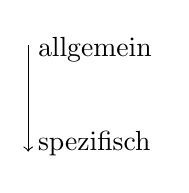
\begin{tikzpicture}
\node[right] at (0,0){spezifisch};
\node[right] at (0,1.2){allgemein};
\draw[<-] (0,-.1)--(0,1.25);
%\draw[<-] (0,.3)--(0,1);
\end{tikzpicture}

\end{minipage}

\begin{itemize}
	\item Notation verschiedener \textbf{Kontexte}:
	\begin{itemize}
		\item Silbengrenze: \$ oder: Silbenanfang: $_\sigma[$ und Silbenende: $]_\sigma$
		\item betonte Silbe: \textprimstress$\sigma$
		\item Koda: \underline{\quad}$_{\textsubscript{K}}$
		\item Morphemgrenze ($=$ Morphemanfang bzw.\ -ende): $+$
		\item Wortgrenze: \#
		\item \{ \dots\ ; \dots\ \} Liste von Kontexten, von denen nur einer gegeben sein muss
	\end{itemize}

\end{itemize}

\end{frame}


%%%%%%%%%%%%%%%%%%%%%%%%%%%%%%%%%
\subsection{Hausaufgabe}
%%%%%%%%%%%%%%%%%%%%%%%%%%%%%%%%%

\begin{frame}
\frametitle{Hausaufgabe}
\begin{itemize}
	\item[1.] Ordnen Sie die Artikulationsorte und -organe (Buchstaben) den entsprechenden Bezeichnungen (Klammern) zu.
	
\begin{minipage}{0.48\textwidth}
	\begin{figure}
		\centering
		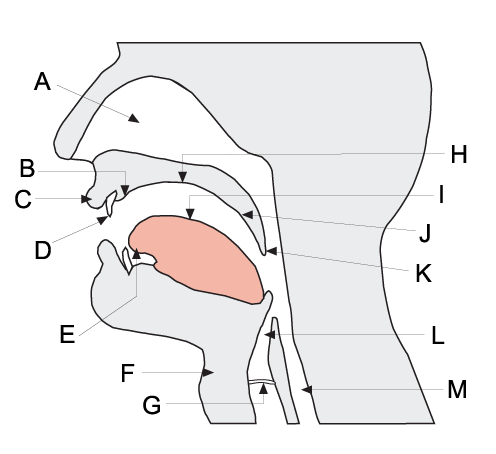
\includegraphics[scale=0.33]{material/04phonoatonomy}
	\end{figure}
\end{minipage}
\hfill
\begin{minipage}{0.4\textwidth}
	
		(~~) Stimmritze (glottal)\\
		(~~) Kehlkopf (laryngal)\\
		(~~) Zahndamm (alveolar)\\
		(~~) Nasenraum (nasal)\\
		(~~) harter Gaumen (palatal)\\
		(~~) Zähne (dental)\\
		(~~) weicher Gaumen (velar)\\
		(~~) Zungenrücken (dorsal)\\
		(~~) Halszäpfchen (uvular)\\
		(~~) Lippen (labial)\\
		(~~) Zungenspitze (apikal)
\end{minipage}

\end{itemize}
\end{frame}


%%%%%%%%%%%%%%%%%%%%%%%%%%%%%%%%
\begin{frame}{Hausaufgabe}
\begin{itemize}
	\item[2.] Welcher Laut passt jeweils nicht in die folgenden Reihen?\\
                  Begründen Sie Ihre Entscheidungen.
	
	\ea \label{ex:03aHA2}
		\ea \textipa{[b]}, \textipa{[z]}, \textipa{[a]}, \textipa{[g]}, \textipa{[v]}, \textipa{[p]}, \textipa{[u]}
		\ex \textipa{[t]}, \textipa{[s]}, \textipa{[n]}, \textipa{[\c{c}]}, \textipa{[l]}, \textipa{[d]}, \textipa{[r]}
		\ex \textipa{[f]}, \textipa{[s]}, \textipa{[x]}, \textipa{[h]}, \textipa{[r]}, \textipa{[z]}
		\ex \textipa{[N]}, \textipa{[m]}, \textipa{[k]}, \textipa{[g]}
		\ex \textipa{[m]}, \textipa{[b]}, \textipa{[N]}, \textipa{[p]}
		\z
	\z
	
	\item[3.] Geben Sie die \textbf{phonologische Repräsentation} der folgenden Wörter und \textbf{verschiedene phonetische Realisierungen} (\zB im Paradigma) an und \textbf{erläutern} Sie anschließend den \textbf{Unterschied} zwischen letzteren.
	
	\ea \label{ex:03aHA3}
		\ea Dieb
		\ex König
		\ex eng
		\z
	\z
	
\end{itemize}

\end{frame}


%%%%%%%%%%%%%%%%%%%%%%%%%%%%%%%%%
\begin{frame}{Hausaufgabe}

\begin{itemize}
	\item[4.] Bestimmen Sie, ob es sich bei den folgenden Lautkombinationen um Affrikaten handeln kann. Begründen Sie Ihre Entscheidungen.
	
	\ea \label{ex:03aHA4}
		\ea \textipa{[kl]}
		\ex \textipa{[pf]}
		\ex \textipa{[st]}
		\ex \textipa{[tr]}
		\ex \textipa{[ts]}
		\z
	\z
	
\end{itemize}

\end{frame}


%%%%%%%%%%%%%%%%%%%%%%%%%%%%%%%%%
\iftoggle{ha-loesung}{
	%%%%%%%%%%%%%%%%%%%%%%%%%%%%%%%%%%
%% HA 1 - 03a Phonologie
%%%%%%%%%%%%%%%%%%%%%%%%%%%%%%%%%%

\begin{frame}
\frametitle{Hausaufgabe -- Lösung}
\begin{itemize}
	\item[1.] Ordnen Sie die Artikulationsorte und -organe (Buchstaben) den entsprechenden Bezeichnungen (Klammern) zu.
	
	\begin{minipage}{0.48\textwidth}
		\begin{figure}
			\centering
			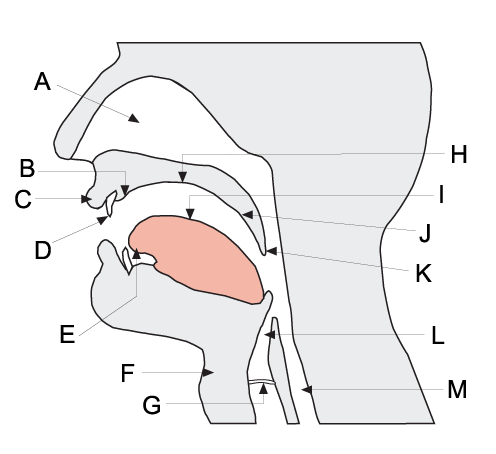
\includegraphics[scale=0.33]{material/04phonoatonomy}
		\end{figure}
	\end{minipage}
	\hfill
	\begin{minipage}{0.4\textwidth}
		
		(\visible<2->{\alertgreen{G}}) Stimmritze (glottal)\\
		(\visible<3->{\alertgreen{F}}) Kehlkopf (laryngal)\\
		(\visible<4->{\alertgreen{B}}) Zahndamm (alveolar)\\
		(\visible<5->{\alertgreen{A}}) Nasenraum (nasal)\\
		(\visible<6->{\alertgreen{H}}) harter Gaumen (palatal)\\
		(\visible<7->{\alertgreen{D}}) Zähne (dental)\\
		(\visible<8->{\alertgreen{J}}) weicher Gaumen (velar)\\
		(\visible<9->{\alertgreen{I}}) Zungenrücken (dorsal)\\
		(\visible<10->{\alertgreen{K}}) Halszäpfchen (uvular)\\
		(\visible<11->{\alertgreen{C}}) Lippen (labial)\\
		(\visible<12->{\alertgreen{E}}) Zungenspitze (apikal)
	\end{minipage}
	
\end{itemize}
\end{frame}


%%%%%%%%%%%%%%%%%%%%%%%%%%%%%%%%
\begin{frame}{Hausaufgabe -- Lösung}
\begin{itemize}
	\item[2.] Welcher Laut passt jeweils nicht in die folgenden Reihen?\\Begründen Sie Ihre Entscheidungen.
	
\begin{exe}
	\exr{ex:03aHA2}
\settowidth\jamwidth{XXXXXXXXXXXXXXXXXXXXXXXt}
	\begin{xlist}
		\ex \textipa{[b]}, \textipa{[z]}, \textipa{[a]}, \textipa{[g]}, \textipa{[v]}, \textipa{[p]}, \textipa{[u]} \loesung{2}{\textipa{[p]} (nicht sth., sondern stl.)}
		\ex \textipa{[t]}, \textipa{[s]}, \textipa{[n]}, \textipa{[\c{c}]}, \textipa{[l]}, \textipa{[d]}, \textipa{[r]} \loesung{3}{\textipa{[ç]} (nicht alveolar, sondern palatal)}
		\ex \textipa{[f]}, \textipa{[s]}, \textipa{[x]}, \textipa{[h]}, \textipa{[r]}, \textipa{[z]}
		\loesung{4}{\textipa{[r]} (kein Frikativ, sondern Vibrant)}
		\ex \textipa{[N]}, \textipa{[m]}, \textipa{[k]}, \textipa{[g]}
		\loesung{5}{\textipa{[k]} (nicht sth., sondern stl.)}\loesung{6}{oder: \textipa{[m]} (nicht velar, sondern labial)}
		\ex \textipa{[m]}, \textipa{[b]}, \textipa{[N]}, \textipa{[p]}
		\loesung{7}{\textipa{[N]} (nicht labial, sondern velar)} \loesung{8}{oder: \textipa{[p]} (nicht sth., sondern stl.)}
	\end{xlist}
\end{exe}
	
\end{itemize}
\end{frame}


%%%%%%%%%%%%%%%%%%%%%%%%%%%%%%%%
\begin{frame}{Hausaufgabe -- Lösung}
\begin{itemize}
	\item[3.] Geben Sie die \textbf{phonologische Repräsentation} der folgenden Wörter und \textbf{verschiedene phonetische Realisierungen} (\zB im Paradigma) an und \textbf{erläutern} Sie anschließend den \textbf{Unterschied} zwischen letzteren.
	
\begin{exe}
	\exr{ex:03aHA3}
	\settowidth\jamwidth{XXXXXXXXXXXXXXXXXXXXXXXXXXXXXXXXXXXXXXt}
	\begin{xlist}
		\ex Dieb
		\loesung{2}{\textipa{/di:b/}: \textipa{[di:p], [di:.bə]} -- Auslautverhärtung des \textipa{/b/} in der Koda}
		\ex König
		\loesung{3}{\textipa{/k\o :nıg/}: \textipa{[k\super h\o:.nıç], [k\super h\o:.nı.gə]} --} \loesung{3}{Spirantisierung des \textipa{/g/} in der Koda}
		\ex eng
		\loesung{4}{\textipa{/εng/}: \textipa{[PεN]}, \textipa{[PENk]} --}
		
		\loesung{4}{ g-Tilgung bzw. (dialektal) Auslautverhärtung}
	\end{xlist}
\end{exe}

\end{itemize}

\end{frame}


%%%%%%%%%%%%%%%%%%%%%%%%%%%%%%%%%
\begin{frame}{Hausaufgabe -- Lösung}

\begin{itemize}
	\item[4.] Bestimmen Sie, ob es sich bei den folgenden Lautkombinationen um Affrikaten handeln kann. Begründen Sie Ihre Entscheidungen.

\begin{exe}	
	\exr{ex:03aHA4}
\settowidth\jamwidth{XXXXXXXXXXXXXXXXXXXXXXXXXXXXXXXXXXXXXXX}
	\begin{xlist}
		\ex \textipa{[kl]} \loesung{2}{keine Affrikate (Zweitglied ist kein Frikativ)}
		\ex \textipa{[pf]} \loesung{3}{Affrikate (Verbindung aus Plosiv und homorganem Frikativ)}
		\ex \textipa{[st]} \loesung{4}{keine Affrikate (Plosiv ist Zweitglied)}
		\ex \textipa{[tr]} \loesung{5}{keine Affrikate (Zweitglied ist kein Frikativ)}
		\ex \textipa{[ts]} \loesung{6}{Affrikate (Verbindung aus Plosiv und homorganem Frikativ)}
	\end{xlist}
\end{exe}

\end{itemize}

\end{frame}



}
%%%%%%%%%%%%%%%%%%%%%%%%%%%%%%%%%


	\exewidth{(235)}
%%%%%%%%%%%%%%%%%%%%%%%%%%%%%%%%%%%%%%%%%%%%%%%%
%% Compile the master file!
%% 		Slides: Antonio Machicao y Priemer
%% 		Course: GK Linguistik
%%%%%%%%%%%%%%%%%%%%%%%%%%%%%%%%%%%%%%%%%%%%%%%%

%\exewidth{(35)} im übergeordneten File

% sollte zentral geladen werden. St. Mü. 04.11.2016 (in localcommands?)
%%%%%%%%%%%%%
%%% Forestset Syllables

\newbox\foreststrutbox
\setbox\foreststrutbox=\hbox to 0pt{\phantom{\forestOve{standard node}{content}}}
\def\foreststrut{\copy\foreststrutbox}
\forestset{
GP1/.style 2 args={
for n={1}{baseline},
s sep=0pt, l sep=0pt,
for descendants={
l sep=0pt, l={#1},
anchor=base,calign=first,child anchor=north,
inner xsep=1pt,inner ysep=2pt,outer sep=0pt,s sep=0pt,
},
delay={
if content={}{phantom}{for children={no edge}},
for tree={
if content={O}{tier=OR}{},
if content={R}{tier=OR}{},
if content={N}{tier=N}{},
if content={x}{
tier=x,content={$\times$},outer xsep={#2},
for tree={calign=center},
for descendants={content format={\foreststrut\forestoption{content}}},
before drawing tree={outer xsep=0pt,delay={typeset node}},
s sep=4pt
}{},
},
},
before drawing tree={where content={}{parent anchor=center,child anchor=center}{}},
},
GP1/.default={5ex}{8.0pt},
associate/.style={%
tikz+={\draw(!)--(!#1);}},
spread/.style={
before drawing tree={tikz+={\draw[dotted](!)--(!#1);}}},
govern/.style={
before drawing tree={tikz+={\draw[->](!)--(!#1);}}},
p-govern/.style={
before drawing tree={tikz+={\draw[->](.north) to[out=150,in=30] (!#1.north);}}},
no p-govern/.style={
before drawing tree={tikz+={\draw[->,loosely dashed](.north) to[out=150,in=30] (!#1.north);}}},
encircle/.style={before drawing tree={circle,draw,inner sep=0pt}},
fen/.style={pin={[font=\footnotesize,inner sep=1pt,pin edge=<-]10:\textsc{Fen}}},
el/.style={content=\textsc{\textbf{##1}}},
head/.style={content=\textsc{\textbf{\underline{##1}}}},
llap/.style={
tikz+={%
\edef\forest@temp{\noexpand\node[\option{node options},
anchor=base east,at=(.base east)]}%
\forest@temp{#1\phantom{\option{environment}}};
}
},
rlap/.style={
tikz+={%
\edef\forest@temp{\noexpand\node[\option{node options},
anchor=base west,at=(.base west)]}%
\forest@temp{\phantom{\option{environment}}#1};
}
},
}
%%%%%%%%%%%%%


%%%%%%%%%%%%%%%%%%%%%%%%%%%%%%%%%%%%%%%%%%%%%%%%%%%%
%%%             Metadata                         
%%%%%%%%%%%%%%%%%%%%%%%%%%%%%%%%%%%%%%%%%%%%%%%%%%%% 

\title{Grundkurs Linguistik}

\subtitle{Phonologie II: Silbe}

\author[A. Machicao y Priemer]{
	{\small Antonio Machicao y Priemer}
	\\
	{\footnotesize \url{http://www.linguistik.hu-berlin.de/staff/amyp}}
	%	\\
	%	\href{mailto:mapriema@hu-berlin.de}{mapriema@hu-berlin.de}}
}

\institute{Institut für deutsche Sprache und Linguistik}


% bitte lassen, sonst kann man nicht sehen, von wann die PDF-Datei ist.
%\date{ }

%\publishers{\textbf{6. linguistischer Methodenworkshop \\ Humboldt-Universität zu Berlin}}

%\hyphenation{nobreak}


%%%%%%%%%%%%%%%%%%%%%%%%%%%%%%%%%%%%%%%%%%%%%%%%%%%%
%%%             Preamble's End                  
%%%%%%%%%%%%%%%%%%%%%%%%%%%%%%%%%%%%%%%%%%%%%%%%%%%%   


%%%%%%%%%%%%%%%%%%%%%%%%%   
\huberlintitlepage[22pt]
\iftoggle{toc}{
\frame{
%\begin{multicols}{2}
	\frametitle{Inhaltsverzeichnis}
	\tableofcontents
	%[pausesections]
%\end{multicols}
}
}

%%%%%%%%%%%%%%%%%%%%%%%%%%%%%%%%%%
%%%%%%%%%%%%%%%%%%%%%%%%%%%%%%%%%%
%%%%%LITERATURE:

%% Allgemein
\nocite{Glueck&Roedel16a}
\nocite{Schierholz&Co18}
\nocite{Luedeling2009a}
\nocite{Meibauer&Co07a} 
\nocite{Repp&Co15a} 

%%% Sprache & Sprachwissenschaft
%\nocite{Fries16c} %Adäquatheit
%\nocite{Fries16a} %Grammatikalität
%\nocite{Fries&MyP16c} %GG
%\nocite{Fries&MyP16b} %Akzeptabilität
%\nocite{Fries&MyP16d} %Kompetenz vs. Performanz

%% Phonetik & Phonologie
\nocite{Altmann&Co07a}
\nocite{DudenAussprache00a}
\nocite{Hall00a} 
\nocite{Kohler99a}
\nocite{Krech&Co09a}
\nocite{Pompino95a}
\nocite{Ramers08a}
\nocite{Ramers&Vater92a}
\nocite{Rues&Co07a}
\nocite{WieseR96a}
\nocite{WieseR11a}


%%%%%%%%%%%%%%%%%%%%%%%%%%%%%%%%%%
%%%%%%%%%%%%%%%%%%%%%%%%%%%%%%%%%%
\section{Phonologie II: Silbe}
%%%%%%%%%%%%%%%%%%%%%%%%%%%%%%%%%%

%@EE: Checken: Struktur -- Reihenfolge der Folien
%@EE: Checken: Inhaltsverzeichnisse usw.
%@EE: Checken: wenn 3b und 3c stehen, kann der auskommentierte Text am Ende von 3b gelöscht werden

%%%%%%%%%%%%%%%%%%%%%%%%%%%%%%%%%%

\begin{frame}
\frametitle{Begleitlektüre}

\begin{itemize}
	\item \textbf{obligatorisch:}
	\begin{itemize}
		\item[] AM S.~18--23
	\end{itemize}
	\item \textbf{optional:}
	\begin{itemize}
		\item[] \citet{Hall00a}: Kapitel~8 (S.~205--230)
	\end{itemize}
\end{itemize}

\end{frame}


%%%%%%%%%%%%%%%%%%%%%%%%%%%%%%%%%%%%
%%%%%%%%%%%%%%%%%%%%%%%%%%%%%%%%%
\subsection{Einführung}

%% MyP: Contents
\iftoggle{sectoc}{
	\frame{
		%\begin{multicols}{2}
		\frametitle{~}
		\tableofcontents[currentsubsection, subsubsectionstyle=hide]
		%\end{multicols}
	}
}

%% StM: Contents
\iftoggle{gliederung}{
	
	\outline{
		\begin{itemize}
			
			\item \blaubf{Einführung}
			\item Silbenbestimmung
			\item Silbenstruktur
			%% Onset
			%% Nukleus
			%% Koda
			\item Phonotaktik
			%% Sonoritätshierarchie
			%% Weitere phonotaktische Beschränkungen
			\item Hausaufgabe
			
		\end{itemize}
	}
}
%%%%%%%%%%%%%%%%%%%%%%%%%%%%%%%%%%%
\begin{frame}
\frametitle{Einführung: Notation}


\begin{itemize}
	\item graphematische Notation in spitzen Klammern: 
	
	  \ea
          \ab{nordwind}, \ab{Nordwind}
          \z
% zwei Varianten, eine phonographisches Prinzip, eine mit syntaktischer Info = Großschreibung
          
	\item[]	
	\item phonetische Notation in eckigen Klammern:
	
	  \ea
          \textipa{[nO5t.vInt]}
	  \z
          
	\item[]
	\item phonologische Notation in Schrägstrichen:
	
	  \ea
          \textipa{/nO\textscr d.vInd/}
	  \z
\end{itemize}

\end{frame}



%%%%%%%%%%%%%%%%%%%%%%%%%%%%%%%%%%%
\begin{frame}
\frametitle{Silben}

Warum nimmt man Silben an?

\begin{itemize}
	\item Die Auslautverhärtung mit Bezug auf das Wort (vorläufig):
	
	\ea {}[$-$son] $\rightarrow$ [$-$sth] /\_\_ \#
             
	{\small (ein nicht-sonoranter Laut -- d.\,h.\ Obstruent -- wird am Wortende nicht-stimmhaft)}
	\z
     
	\item Transkribieren Sie: (\emph{sie}) \emph{siegte}

% Auslautverhärtung auch bei Silben
\pause	

	\ea
	\textipa{[zi:k . t@]} (\gqq{.} steht für Silbengrenze)
	\z

%\pause
%
%	\eal 
%	\ex \textipa{[St\textscr e:p.za:m]} \vs \textipa{[St\textscr e:.b5]}
%	\ex \textipa{[bYnt.nIs]} \vs \textipa{[bUn.d@s]}
%	\ex \textipa{[bi:k.za:m]} \vs \textipa{[bi:.g@n]}
%	\ex \textipa{[le:s.b5]} \vs \textipa{[le:.z@n]}
%    \zl
%        
%	\item Auslautverhärtung mit Bezug auf die \textbf{Silbe}:
%	  \ea
%             {}[$-$son] $\rightarrow$ [$-$sth] /\_\_ $]_{\sigma}$
%	  \z	
\end{itemize}

\end{frame}


%%%%%%%%%%%%%%%%%%%%%%%%%%%%%%%%%%%
\begin{frame}
\frametitle{Silben}

\begin{itemize}
	\item Vergleichen Sie:

\ea 

\begin{tabular}[t]{lllclll}
\only<1->{a. \ab{stre\alertred{b}sam} & \vs & \ab{Stre\alertred{b}er} &} \only<2->{~ & \textipa{[St\textscr e:\alertred{p}.za:m]} & \vs & \textipa{[St\textscr e:.\alertred{b}5]}}\\

\only<1->{b. \ab{Bün\alertred{d}nis} & \vs & \ab{Bun\alertred{d}es} &} \only<3->{~ & \textipa{[bYn\alertred{t}.nIs]} & \vs & \textipa{[bUn.\alertred{d}@s]}}\\

\only<1->{c. \ab{bie\alertred{g}sam} & \vs & \ab{bie\alertred{g}en} &} \only<4->{& \textipa{[bi:\alertred{k}.za:m]} & \vs &  \textipa{[bi:.\alertred{g}@n]}} \\

\only<1->{d. \ab{le\alertred{s}bar} & \vs & \ab{le\alertred{s}en} &} \only<5->{& \textipa{[le:\alertred{s}.b5]} & \vs &  \textipa{[le:.\alertred{z}@n]}} \\

\end{tabular}

\z 

%\begin{columns}
%\begin{column}[t]{.5\linewidth}
%\eal 
%	\ex \ab{stre\alertred{b}sam} \vs \ab{Stre\alertred{b}er}
%	\ex \ab{Bün\alertred{d}nis} \vs \ab{Bun\alertred{d}es} 
%	\ex \ab{bie\alertred{g}sam} \vs \ab{bie\alertred{g}en}
%	\ex \ab{le\alertred{s}bar} \vs \ab{le\alertred{s}en}
%\zl	
%\end{column}
%
%%\pause 
%
%\begin{column}[t]{\linewidth}
%\begin{itemize}
%%\eal 
%%\ex 
%	\item[] \textipa{[St\textscr e:\alertred{p}.za:m]} \vs \textipa{[St\textscr e:.\alertred{b}5]}
%%\ex 
%	\item[] \textipa{[bYn\alertred{t}.nIs]} \vs \textipa{[bUn.\alertred{d}@s]}
%%\ex 
%	\item[] \textipa{[bi:\alertred{k}.za:m]} \vs \textipa{[bi:.\alertred{g}@n]}
%%\ex 
%	\item[] \textipa{[le:\alertred{s}.b5]} \vs \textipa{[le:.\alertred{z}@n]}
%%\zl
%\end{itemize}
%\end{column}
%
%\end{columns}	
\end{itemize}


\begin{itemize}
	\item<6-> Auslautverhärtung mit Bezug auf die \textbf{Silbe}:
	\ea
	{}[$-$son] $\rightarrow$ [$-$sth] /\_\_ $]_{\sigma}$
	\z	
\end{itemize}

\end{frame}


%%%%%%%%%%%%%%%%%%%%%%%%%%%%%%%%%%%
\begin{frame}
\frametitle{Silben}

Warum nimmt man Silben an?

Silbe als \textbf{Domäne} \ldots

\begin{itemize}	
	\item \ldots\ verschiedener \textbf{phonologischer Prozesse}\\
               (\zB Auslautverhärtung, Knacklauteinsetzung, Aspiration, \ldots )
	
	\item[] 
	
	\item \ldots\ von Regularitäten bzgl. der \textbf{Abfolge} von Lauten
	
	\item[]
	
	\item \ldots\ der \textbf{Wortbetonung}, d.\,h. wichtige so genannte prosodische Einheiten (Prosodie $=$ Betonung mit Bezug auf Einheiten über dem Segment)
\end{itemize}

\end{frame}



%%%%%%%%%%%%%%%%%%%%%%%%%%%%%%%%%%%
%
%\begin{frame}
%\frametitle{Prosodische Konstituenten}
%
%
%	\begin{multicols}{2}
%	\begin{itemize*}
%		\item UP = Äußerungsphrase
%		\item IP = Intonationsphrase
%		\item $\phi$ = phonol. Phrase
%\columnbreak
%		\item $\omega$ = phonol. Wort
%		\item F = phonol. Fuß
%		\item \alertred{$\sigma$ = Silbe}
%	\end{itemize*}
%	\end{multicols}
%
%\begin{figure} %%rote Box einfügen
%	\centering
%	\scalebox{.68}{
%	\begin{forest} MyP edges,
%	[IP
%	[$\Phi$
%	[$\omega$[F[\alertred{$\sigma$}[Frau]]]]
%	[$\omega$[F[\alertred{$\sigma$}[Müll, name=mueller]][\alertred{$\sigma$}, name=sigma[er]]]]]
%	[$\Phi$
%	[$\omega$[F[\alertred{$\sigma$}[kauft]]]]
%	[$\omega$[F[\alertred{$\sigma$}[Steck]]]
%			 [F[\alertred{$\sigma$}[rü]]
%			   [\alertred{$\sigma$}[ben]]]]]
%	[$\Phi$
%	[$\omega$[F[\alertred{$\sigma$}[auf]]]
%			 [F[\alertred{$\sigma$}[dem]]]]
%	[$\omega$[F[\alertred{$\sigma$}[Woch, name=woch]]
%			   [\alertred{$\sigma$}, name=sigmab[en]]]
%			 [F[\alertred{$\sigma$}[markt]]]]]
%	]
%	{
%		\draw[black] (mueller.north)--(sigma.south);
%		\draw[black] (woch.north)--(sigmab.south);
%	}
%	\end{forest}
%}
%	\caption{nach C. Féry}
%	\label{Zeichen1}
%\end{figure}
%
%% Doppeltverwendung bei Silbengelenken Mül ler
%
%% betonte Silben bilden Fuß einschließlich allen folgenden unbetonten Silben
%
%%\begin{figure}[b]
%%	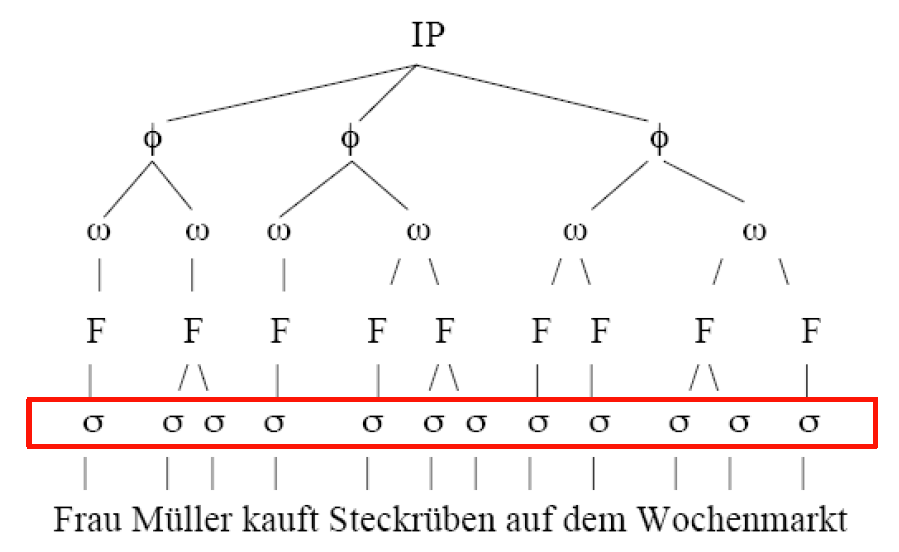
\includegraphics[scale=0.3]{material/03bHierarchieIntonationsphrase}
%%	\caption{Hierarchie in der Intonationsphrase (Darstellung von C. Féry)}
%%	\label{Zeichen1}
%%\end{figure}
%
%\end{frame}

%%%%%%%%%%%%%%%%%%%%%%%%%%%%%%%%%%%
\begin{frame}
\frametitle{Prosodische Konstituenten}

	\begin{multicols}{2}
	\begin{itemize*}
		\item UP = Äußerungsphrase
		\item IP = Intonationsphrase
		\item $\varphi$ = phonol. Phrase
\columnbreak
		\item $\omega$ = phonol. Wort
		\item F = phonol. Fuß
		\item \alertred{$\sigma$ = Silbe}
	\end{itemize*}
	\end{multicols}


	\begin{figure}
	\centering
	\scalebox{.68}{
		\begin{forest} MyP edges,
		[UP, name=up
		[IP, name=IP
		[$\varphi$[$\omega$[F[$\sigma$][$\sigma$]][F[$\sigma$][$\sigma$]]]]
		[$\varphi$, name=Phi[$\omega$[F[$\sigma$][$\sigma$]]][$\omega$, name=omega[F, name=F[$\sigma$][$\sigma$, name=sigma]]]]
		]]
		{\draw[black] (up.east)--(3,0);
			\draw[black] (IP.east)--(3,-1);
			\draw[black] (Phi.east)--(3,-2);
			\draw[black] (omega.east)--(3,-3);
			\draw[black] (F.east)--(3,-4);
			\draw[black] (sigma.east)--(3,-5.3);
			\node[right] at (3,0) {(Mandarinen oder Äpfel)\textsubscript{UP}};
			\node[right] at (3,-1) {(Mandarinen oder Äpfel)\textsubscript{IP}};
			\node[right] at (3,-2) {(Mandarinen)\textsubscript{$\varphi$} (oder Äpfel)\textsubscript{$\varphi$}};
			\node[right] at (3,-3) {(Mandarinen)\textsubscript{$\omega$} (oder)\textsubscript{$\omega$} (Äpfel)\textsubscript{$\omega$}};
			\node[right] at (3,-4) {(Manda)\textsubscript{F} (rinen)\textsubscript{F} (oder)\textsubscript{F} (Äpfel)\textsubscript{F}};
			\node[right] at (3,-5.3) {(Man)\textsubscript{$\sigma$} (da)\textsubscript{$\sigma$} (ri)\textsubscript{$\sigma$} (nen)\textsubscript{$\sigma$} (o)\textsubscript{$\sigma$} (der)\textsubscript{$\sigma$} (Äp)\textsubscript{$\sigma$} (fel)\textsubscript{$\sigma$}};
	}
		\end{forest}
	}
		\caption{\cite{Fuhrhop&Co13a}}
	\end{figure}

%\begin{figure}[b]
%	\centering
%	
%	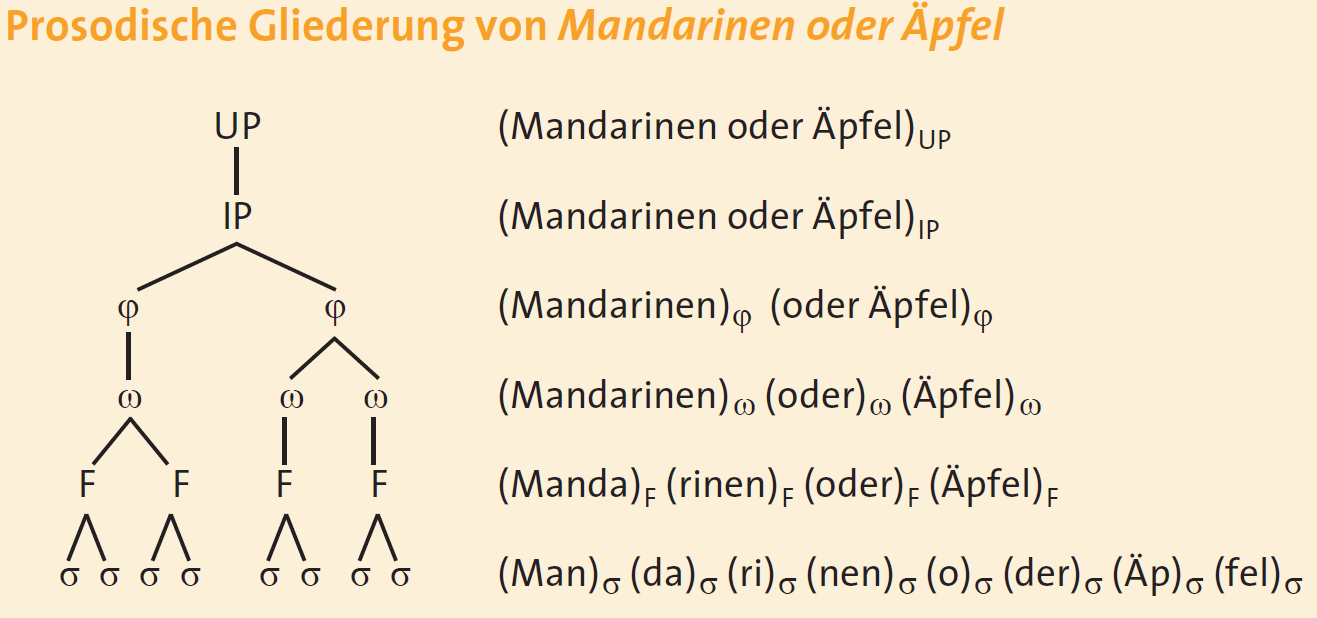
\includegraphics[scale=0.26]{material/03bHierarchieUP}
%	\caption{Hierarchie in der Äußerungsphrase \citep[8]{Fuhrhop&Co13a}}
%	%\label{Zeichen1}
%\end{figure}

\end{frame}


%%%%%%%%%%%%%%%%%%%%%%%%%%%%%%%%%%
%%%%%%%%%%%%%%%%%%%%%%%%%%%%%%%%%%
\subsection{Silbenbestimmung}

%% MyP: Contents
\iftoggle{sectoc}{
	\frame{
		%\begin{multicols}{2}
		\frametitle{~}
		\tableofcontents[currentsubsection, subsubsectionstyle=hide]
		%\end{multicols}
	}
}

%% StM: Contents
\iftoggle{gliederung}{
	
	\outline{
		\begin{itemize}
			
			\item Einführung
			\item \blaubf{Silbenbestimmung}
			\item Silbenstruktur
			%% Onset
			%% Nukleus
			%% Koda
			\item Phonotaktik
			%% Sonoritätshierarchie
			%% Weitere phonotaktische Beschränkungen
			\item Hausaufgabe
			
		\end{itemize}
	}
}
%%%%%%%%%%%%%%%%%%%%%%%%%%%%%%%%%%

\begin{frame}
\frametitle{Silbenbestimmung}

\begin{itemize}
	\item<1-> Wie viele Silben hat das folgende Wort?
	
	\ea Silbenbestimmung
	\z
	
	\item<2-> Woher wissen Sie das?
	
	\begin{itemize}
		\item[]<2-> \gqq{Jeder kompetente Sprachteilhaber verfügt über die \textbf{Fähigkeit},\\
 Silben identifizieren zu können.}  \citep[133]{Staffeldt10a}

		\vspace{.25cm}

		\item[]<2-> \gqq{Silbe: Phonetisch-phonologische \textbf{Grundeinheit} des Wortes
                  bzw.\ der Rede, die zwar \textbf{intuitiv} nachweisbar ist, wissenschaftlich aber \textbf{nicht einheitlich definiert} wird.} \citep[600]{Bussmann02a}
		
	\end{itemize}
 
	\item<3-> Silben können \textbf{betont} werden (tragen Akzent)
	
	\item<4-> \textbf{Silbenspiele} (\zB \only<5->{Sil\alertred{pi}-ben\alertred{pe}-spie\alertred{pi}-le\alertred{pe},} \only<5->{Si\alertred{hi}l-be\alertred{he}n-spie\alertred{hi}-le\alertred{he})}
% Geheimsprache, nach Silben wird immer pi, pa, pe oder so eingesetzt
	
	\item<6-> \textbf{Intuitiv} erkennbare Einheit: 
	
	Kinder können in einem sehr frühen Alter intuitiv Silben klatschen.

\end{itemize}

\end{frame}



%%%%%%%%%%%%%%%%%%%%%%%%%%%%%%%%%%
%%%%%%%%%%%%%%%%%%%%%%%%%%%%%%%%%%
\subsection{Silbenstruktur}

%% MyP: Contents
\iftoggle{sectoc}{
	\frame{
		%\begin{multicols}{2}
		\frametitle{~}
		\tableofcontents[currentsubsection, subsubsectionstyle=hide]
		%\end{multicols}
	}
}

%% StM: Contents
\iftoggle{gliederung}{
	
	\outline{
		\begin{itemize}
			
			\item Einführung
			\item Silbenbestimmung
			\item \blaubf{Silbenstruktur}
			%% Onset
			%% Nukleus
			%% Koda
			\item Phonotaktik
			%% Sonoritätshierarchie
			%% Weitere phonotaktische Beschränkungen
			\item Hausaufgabe
			
		\end{itemize}
	}
}
%%%%%%%%%%%%%%%%%%%%%%%%%%%%%%%%%%
\begin{frame}
\frametitle{Silbenstruktur}

\begin{itemize}
	\item Welche Silben (des Deutschen) sind mit den folgenden Segmenten bildbar?

\ea \textipa{[p]}, \textipa{[a]}, \textipa{[l]}, \textipa{[t]}
\z

\pause	

\begin{multicols}{2}
\ea \textbf{bildbar:}\\
	\textipa{[palt]},\\
	\textipa{[alpt]}, \\
	\textipa{[lapt]}, \\
	\textipa{[talp]}, \\
	\textipa{[plat]}
\z 

\columnbreak

\pause

	\ea \textbf{nicht bildbar:}\\
	*\textipa{[ltap]}, \\
	*\textipa{[lpat]},\\
	*\textipa{[ptla]}, \\
	*\textipa{[tpal]}, 	\ldots 
\z
\end{multicols}

\pause

\item Warum?

\end{itemize}

\end{frame}



%%%%%%%%%%%%%%%%%%%%%%%%%%%%%%%%%%%
%\begin{frame}
%\frametitle{Silbenstruktur}
%
%Die Silbe ist \textbf{intern strukturiert} und besteht aus den folgenden Teilen:
%
%\begin{minipage}{.60\textwidth}
%
%\begin{itemize}
%	\item[]
%	\item Silbenanlaut/Silbenanfangsrand/\alert{Onset},
%	\begin{itemize}
%		\item 0 bis $n$ Konsonanten, wobei in fast allen Sprachen $n < 5$
%	\end{itemize}
%	
%	\item[]
%	\item Silbengipfel/Silbenkern/\alert{Nukleus},
%	\begin{itemize}
%		\item Vokale
%		\item manchmal (vokalische) Nasale oder Liquide
%	\end{itemize}
%	
%	\item[]
%	\item Silbenauslaut/Silbenendrand/\alert{Koda}
%	\begin{itemize}
%		\item 0 bis $n$ Konsonanten, wobei in fast allen Sprachen $n < 5$
%	\end{itemize}
%
%	\item[]
%	\item Nukleus und Koda bilden den \alert{Reim}
%	
%\end{itemize}
%
%
%\end{minipage}
%\begin{minipage}{.39\textwidth}
%
%%%%%%%%%%%%%%
%%% Forestset Syllables

\newbox\foreststrutbox
\setbox\foreststrutbox=\hbox to 0pt{\phantom{\forestOve{standard node}{content}}}
\def\foreststrut{\copy\foreststrutbox}
\forestset{
GP1/.style 2 args={
for n={1}{baseline},
s sep=0pt, l sep=0pt,
for descendants={
l sep=0pt, l={#1},
anchor=base,calign=first,child anchor=north,
inner xsep=1pt,inner ysep=2pt,outer sep=0pt,s sep=0pt,
},
delay={
if content={}{phantom}{for children={no edge}},
for tree={
if content={O}{tier=OR}{},
if content={R}{tier=OR}{},
if content={N}{tier=N}{},
if content={x}{
tier=x,content={$\times$},outer xsep={#2},
for tree={calign=center},
for descendants={content format={\foreststrut\forestoption{content}}},
before drawing tree={outer xsep=0pt,delay={typeset node}},
s sep=4pt
}{},
},
},
before drawing tree={where content={}{parent anchor=center,child anchor=center}{}},
},
GP1/.default={5ex}{8.0pt},
associate/.style={%
tikz+={\draw(!)--(!#1);}},
spread/.style={
before drawing tree={tikz+={\draw[dotted](!)--(!#1);}}},
govern/.style={
before drawing tree={tikz+={\draw[->](!)--(!#1);}}},
p-govern/.style={
before drawing tree={tikz+={\draw[->](.north) to[out=150,in=30] (!#1.north);}}},
no p-govern/.style={
before drawing tree={tikz+={\draw[->,loosely dashed](.north) to[out=150,in=30] (!#1.north);}}},
encircle/.style={before drawing tree={circle,draw,inner sep=0pt}},
fen/.style={pin={[font=\footnotesize,inner sep=1pt,pin edge=<-]10:\textsc{Fen}}},
el/.style={content=\textsc{\textbf{##1}}},
head/.style={content=\textsc{\textbf{\underline{##1}}}},
llap/.style={
tikz+={%
\edef\forest@temp{\noexpand\node[\option{node options},
anchor=base east,at=(.base east)]}%
\forest@temp{#1\phantom{\option{environment}}};
}
},
rlap/.style={
tikz+={%
\edef\forest@temp{\noexpand\node[\option{node options},
anchor=base west,at=(.base west)]}%
\forest@temp{\phantom{\option{environment}}#1};
}
},
}
%%%%%%%%%%%%%

%\begin{figure}
%\centering
%\begin{forest} MyP edges, GP1 [
%  [$\sigma$
%    [O	[ [C$^{n}$]]
%    ]
%    [R	[N
%    		[V$^{n}$]
%    	]
%    	[K
%    		[C$^{n}$]
%    	]
%    ]
%  ]
%]
%\end{forest}
%\caption{Silbenstruktur}
%\end{figure}
%
%\end{minipage}
%
%\end{frame}



%%%%%%%%%%%%%%%%%%%%%%%%%%%%%%%%%%

\begin{frame}
\frametitle{Silbenstruktur: komplexe Silbe}

Die Silbe ist \textbf{intern strukturiert} und besteht aus den folgenden Teilen:

\begin{minipage}{.59\textwidth}

\begin{itemize}
	\item[]
	\item \alertred{Onset} 
	
	\item \alertred{Reim} 
	
	\item \alertred{Nukleus}
	
	\item \alertred{Koda}
	\item[] 
	\item C $:=$ konsonantisch, d.\,h. nicht-silbisch ($\neq$Konsonant)
	
	\item V $:=$ vokalisch, d.\,h. silbisch ($\neq$Vokal)
	
\end{itemize}


\end{minipage}
\begin{minipage}{.40\textwidth}

%%%%%%%%%%%%%%
%%% Forestset Syllables

\newbox\foreststrutbox
\setbox\foreststrutbox=\hbox to 0pt{\phantom{\forestOve{standard node}{content}}}
\def\foreststrut{\copy\foreststrutbox}
\forestset{
GP1/.style 2 args={
for n={1}{baseline},
s sep=0pt, l sep=0pt,
for descendants={
l sep=0pt, l={#1},
anchor=base,calign=first,child anchor=north,
inner xsep=1pt,inner ysep=2pt,outer sep=0pt,s sep=0pt,
},
delay={
if content={}{phantom}{for children={no edge}},
for tree={
if content={O}{tier=OR}{},
if content={R}{tier=OR}{},
if content={N}{tier=N}{},
if content={x}{
tier=x,content={$\times$},outer xsep={#2},
for tree={calign=center},
for descendants={content format={\foreststrut\forestoption{content}}},
before drawing tree={outer xsep=0pt,delay={typeset node}},
s sep=4pt
}{},
},
},
before drawing tree={where content={}{parent anchor=center,child anchor=center}{}},
},
GP1/.default={5ex}{8.0pt},
associate/.style={%
tikz+={\draw(!)--(!#1);}},
spread/.style={
before drawing tree={tikz+={\draw[dotted](!)--(!#1);}}},
govern/.style={
before drawing tree={tikz+={\draw[->](!)--(!#1);}}},
p-govern/.style={
before drawing tree={tikz+={\draw[->](.north) to[out=150,in=30] (!#1.north);}}},
no p-govern/.style={
before drawing tree={tikz+={\draw[->,loosely dashed](.north) to[out=150,in=30] (!#1.north);}}},
encircle/.style={before drawing tree={circle,draw,inner sep=0pt}},
fen/.style={pin={[font=\footnotesize,inner sep=1pt,pin edge=<-]10:\textsc{Fen}}},
el/.style={content=\textsc{\textbf{##1}}},
head/.style={content=\textsc{\textbf{\underline{##1}}}},
llap/.style={
tikz+={%
\edef\forest@temp{\noexpand\node[\option{node options},
anchor=base east,at=(.base east)]}%
\forest@temp{#1\phantom{\option{environment}}};
}
},
rlap/.style={
tikz+={%
\edef\forest@temp{\noexpand\node[\option{node options},
anchor=base west,at=(.base west)]}%
\forest@temp{\phantom{\option{environment}}#1};
}
},
}
%%%%%%%%%%%%%


\begin{figure}
\centering
\begin{forest} MyP edges, GP1 [
  [$\sigma$
    [O
    	[[C[\textipa{S}]]]
    	[[C[\textipa{t}]]]
    	[[C[\textipa{\textscr}]]]
    ]
    [R
    	[N
    		[V[\textipa{U}]]
    	]
    	[K
    		[C[\textipa{m}]]
    		[C[\textipa{\t{pf}}]]
    		[C[\textipa{s}]]
    		[C[\textipa{t}]]
    	]
    ]
  ]
]
\end{forest}
%\caption{Komplexe Silbe}
\end{figure}
% wahrscheinlich komplexeste Koda, die es gibt.
\end{minipage}

\end{frame}


%%%%%%%%%%%%%%%%%%%%%%%%%%%%%%%%%%
\begin{frame}
\frametitle{Silbenstruktur: minimale Silbe}

Die Silbe ist \textbf{intern strukturiert} und besteht aus den folgenden Teilen:

\begin{minipage}{.60\textwidth}

\begin{itemize}
	\item[]
	\item \alertred{Onset}
	
	\item \alertred{Reim}
	
	\item \alertred{Nukleus}
	
	\item \alertred{Koda}
	\item[] 
	\item \textbf{Minimale Silbe} besteht nur aus einem V im  Nukleus
	  \ea
          \ab{gehe} \ras \textipa{[ge:.\alertred{@}]}
          \z
	
\end{itemize}


\end{minipage}
\begin{minipage}{.39\textwidth}

%%%%%%%%%%%%%%
%%% Forestset Syllables

\newbox\foreststrutbox
\setbox\foreststrutbox=\hbox to 0pt{\phantom{\forestOve{standard node}{content}}}
\def\foreststrut{\copy\foreststrutbox}
\forestset{
GP1/.style 2 args={
for n={1}{baseline},
s sep=0pt, l sep=0pt,
for descendants={
l sep=0pt, l={#1},
anchor=base,calign=first,child anchor=north,
inner xsep=1pt,inner ysep=2pt,outer sep=0pt,s sep=0pt,
},
delay={
if content={}{phantom}{for children={no edge}},
for tree={
if content={O}{tier=OR}{},
if content={R}{tier=OR}{},
if content={N}{tier=N}{},
if content={x}{
tier=x,content={$\times$},outer xsep={#2},
for tree={calign=center},
for descendants={content format={\foreststrut\forestoption{content}}},
before drawing tree={outer xsep=0pt,delay={typeset node}},
s sep=4pt
}{},
},
},
before drawing tree={where content={}{parent anchor=center,child anchor=center}{}},
},
GP1/.default={5ex}{8.0pt},
associate/.style={%
tikz+={\draw(!)--(!#1);}},
spread/.style={
before drawing tree={tikz+={\draw[dotted](!)--(!#1);}}},
govern/.style={
before drawing tree={tikz+={\draw[->](!)--(!#1);}}},
p-govern/.style={
before drawing tree={tikz+={\draw[->](.north) to[out=150,in=30] (!#1.north);}}},
no p-govern/.style={
before drawing tree={tikz+={\draw[->,loosely dashed](.north) to[out=150,in=30] (!#1.north);}}},
encircle/.style={before drawing tree={circle,draw,inner sep=0pt}},
fen/.style={pin={[font=\footnotesize,inner sep=1pt,pin edge=<-]10:\textsc{Fen}}},
el/.style={content=\textsc{\textbf{##1}}},
head/.style={content=\textsc{\textbf{\underline{##1}}}},
llap/.style={
tikz+={%
\edef\forest@temp{\noexpand\node[\option{node options},
anchor=base east,at=(.base east)]}%
\forest@temp{#1\phantom{\option{environment}}};
}
},
rlap/.style={
tikz+={%
\edef\forest@temp{\noexpand\node[\option{node options},
anchor=base west,at=(.base west)]}%
\forest@temp{\phantom{\option{environment}}#1};
}
},
}
%%%%%%%%%%%%%


\begin{figure}
\centering
\begin{forest} MyP edges, GP1 [
  [$\sigma$
    [O
    ]
    [R
    	[N
    		[V[\textipa{@}]]
    	]
    	[K
    	]
    ]
  ]
]
\end{forest}
%\caption{Minimale Silbe}
\end{figure}


\end{minipage}

\end{frame}


%%%%%%%%%%%%%%%%%%%%%%%%%%%%%%%%%%
\begin{frame}
\frametitle{Offene/geschlossene/nackte/bedeckte Silben}

\begin{itemize}
	\item Silbenanlaut/Silbenanfangsrand/\alertred{Onset},
	\item Silbengipfel/Silbenkern/\alertred{Nukleus},
	\item Silbenauslaut/Silbenendrand/\alertred{Koda}
	
\end{itemize}

\begin{table}
\centering
\begin{tabular}{lllll}
\textsc{Onset} & \textsc{Nukleus} & \textsc{Koda} & \textsc{Term} & \textsc{Merkmal} \\
\hline
\textipa{z} & \textipa{e:} & & offene Silbe & Koda: leer\\
\hline
\textipa{t} & \textipa{a:} & \textipa{l} & geschlossene Silbe & Koda: besetzt\\
\hline
 & \textipa{@} & \textipa{n} & nackte Silbe & Onset: leer\\
\hline
\textipa{z} & \textipa{e:} & & bedeckte Silbe & Onset: besetzt\\
\end{tabular}
\end{table}

\end{frame}



%%%%%%%%%%%%%%%%%%%%%%%%%%%%%%%%%
%%%%%%%%%%%%%%%%%%%%%%%%%%%%%%%%%
\subsubsection{Onset}
%\frame{
%\begin{multicols}{2}
%\frametitle{~}
%	\tableofcontents[currentsection]
%\end{multicols}
%}
%%%%%%%%%%%%%%%%%%%%%%%%%%%%%%%%%

\begin{frame}
\frametitle{Onset}

Im Deutschen sind
	\begin{itemize}
		\item \textbf{3 Cs} beschränkt: \textipa{/S/} oder \textipa{/s/} $+$ stl. Plosiv $+$ Liquid (\zB \textbf{Spl}itter, \textbf{Skl}ave),
		\item \textbf{2 Cs} oft (\zB \textipa{/bl/}, \textipa{/kn/} \dots\ ) und
		\item \textbf{1 C} immer (bis auf \textipa{[N]}) möglich.
	\end{itemize}
	
	
Maximale Onset-Belegung in verschiedenen Sprachen:


\eal
\ex Deutsch \textipa{[\alertred{St\textscr}aIt]} \gq{Streit}
\ex Tschechisch \textipa{[\alertred{fspl}a.nout]} \gq{aufflammen}
\ex Hawaianisch \textipa{[a.\alertred{l}o.\alertred{h}a]} \gq{Liebe}
\zl

\end{frame}

%%%%%%%%%%%%%%%%%%%%%%%%%%%%%%%%%%
\begin{frame}
\frametitle{Onset: Silbenanlautgesetz}

\begin{itemize}
	\item Bei Betrachtung aller (bekannten) Sprachen kann man die folgende Gesetzmäßigkeit feststellen \citep[cf.][212f.]{Hall00a}:
	
\medskip
	\begin{block}{Silbenanlautgesetz}
	
	\sub{$\sigma$}[CV $>$ \sub{$\sigma$}[V 
	und
	\sub{$\sigma$}[C\MyPup{$n$}V $>$ \sub{$\sigma$}[C\MyPup{$n+1$}V (wobei $n \geq 1$)
	
	$>$ $:=$ \gq{häufiger als} oder \gq{ist weniger markiert als}

% Silbe mit Konsonant und Vokal sind häfiger als solche, die nur mit Vokal beginnen
% Silbe mit n Konsonanten ist weniger markiert als Silbe mit n+1 KOnsonanten.
	
	\end{block}
\medskip
	 
	 \item Man spricht auch von der \textbf{Markiertheit} von Silben,\\
	 wenn sie Präferenzgesetzen widersprechen.

\end{itemize}

\end{frame}


%%%%%%%%%%%%%%%%%%%%%%%%%%%%%%%%%%
%%%%%%%%%%%%%%%%%%%%%%%%%%%%%%%%%%
\subsubsection{Nukleus}
%\frame{
%\begin{multicols}{2}
%\frametitle{~}
%	\tableofcontents[currentsection]
%\end{multicols}
%}
%%%%%%%%%%%%%%%%%%%%%%%%%%%%%%%%%%

\begin{frame}
\frametitle{Nukleus: Silbenkerngesetz}

\begin{itemize}

	\item In \emph{allen} Sprachen werden Nuklei durch \textbf{Vokale} (V) gebildet.
	
	\item In \emph{einigen} Sprachen können Nuklei auch durch \textbf{Liquide} und \textbf{Nasale} (C \vs V) gebildet werden.

	\item Im Deutschen werden bei schnellem Sprechen folgende Wörter mit sogenannten \textbf{silbischen Konsonanten} gesprochen
	
	\begin{multicols}{2}
          \ea
          \ab{lesen} \textipa{[le:.z\alertred{\textsyllabic{n}}]}
          \z
          
          \ea
          \ab{Wandel} \textipa{[van.d\alertred{\textsyllabic{l}}]}
          \z
	\end{multicols}

\pause 

	\item Bei Betrachtung aller (bekannten) Sprachen kann man die folgende Gesetzmäßigkeit feststellen \citep[cf.][217f.]{Hall00a}:

\end{itemize}
	
	\begin{block}{Silbenkerngesetz}
		
	Vokale $>$ Sonoranten $>$ Obstruenten\\
	Silben mit einfachem vokalischem Nukleus sind universell bevorzugt.
	\end{block}
	
\end{frame}



%%%%%%%%%%%%%%%%%%%%%%%%%%%%%%%%%%
%%%%%%%%%%%%%%%%%%%%%%%%%%%%%%%%%%
\subsubsection{Koda}
%\frame{
%\begin{multicols}{2}
%\frametitle{~}
%	\tableofcontents[currentsection]
%\end{multicols}
%}
%%%%%%%%%%%%%%%%%%%%%%%%%%%%%%%%%%

\begin{frame}
\frametitle{Koda: Silbenauslautgesetz}

In der Koda sind/ist \ldots

\begin{itemize}

	\item \ldots\ in \emph{vielen} Sprachen keine Konsonanten erlaubt (\zB Hawaiianisch),
	
	\item \ldots\ in \emph{einigen} Sprachen ein Konsonant erlaubt,
	
	\item \ldots\ in \emph{einigen (wenigen)} Sprachen mehrere Konsonanten erlaubt.
	
	\item[]
	\item Deutsch: \textipa{[hE\alertred{\textscr psts}]} (0 bis 4/5 Konsonanten)
	
	\item Reihenfolge der Konsonanten unterliegt dem  \textbf{Sonoritätsprinzip}
	
	\item Bei Betrachtung aller (bekannten) Sprachen kann man die folgende Gesetzmäßigkeit feststellen \citep[cf.][214]{Hall00a}:

\end{itemize}
	
	\begin{block}{Silbenauslautgesetz}
	
	CVC$^{n}$]$_{\sigma}$ $>$ CVC$^{n+1}$]$_{\sigma}$ (wobei $n \geq 0$)
	
	\end{block}
	
\end{frame}



%%%%%%%%%%%%%%%%%%%%%%%%%%%%%%%%%%%
%%%%%%%%%%%%%%%%%%%%%%%%%%%%%%%%%%%
\subsection{Phonotaktik}

%% MyP: Contents
\iftoggle{sectoc}{
	\frame{
		%\begin{multicols}{2}
		\frametitle{~}
		\tableofcontents[currentsubsection, subsubsectionstyle=hide]
		%\end{multicols}
	}
}

%% StM: Contents
\iftoggle{gliederung}{
	
	\outline{
		\begin{itemize}
			
			\item Einführung
			\item Silbenbestimmung
			\item Silbenstruktur
			%% Onset
			%% Nukleus
			%% Koda
			\item \blaubf{Phonotaktik}
			%% Sonoritätshierarchie
			%% Weitere phonotaktische Beschränkungen
			\item Hausaufgabe			
			
		\end{itemize}
	}
}
%%%%%%%%%%%%%%%%%%%%%%%%%%%%%%%%%%

\begin{frame}
\frametitle{Phonotaktik}

\begin{block}{Phonotaktik}

Die Phonotaktik untersucht die syntagmatischen Beziehungen zwischen Lauten innerhalb der Silbe und anderer prosodischer Einheiten \citep{Fuhrhop&Co13a}.

\end{block}

\begin{itemize}
	\item Mögliche und unmögliche Kombinationen von Segmenten bzgl.
	
	\begin{itemize}
		\item Anzahl der Laute,
		\item Art,
		\item Reihenfolge der Laute.
	\end{itemize}

\end{itemize}

\end{frame}



%%%%%%%%%%%%%%%%%%%%%%%%%%%%%%%%%%
%%%%%%%%%%%%%%%%%%%%%%%%%%%%%%%%%%
\subsubsection{Sonoritätshierarchie}
%\frame{
%\begin{multicols}{2}
%\frametitle{~}
%	\tableofcontents[currentsection]
%\end{multicols}
%}
%%%%%%%%%%%%%%%%%%%%%%%%%%%%%%%%%%

\begin{frame}
\frametitle{Sonoritätshierarchie}

\begin{itemize}
	\item Betrachten Sie die folgenden Beispiele und überlegen Sie \ldots
	
	\begin{enumerate}
		\item \ldots\ welche \textbf{phonotaktischen Beschränkungen} für den Onset in deutschen Silben gelten könnten:

                  \ea
                  \textipa{[\alertred{k\textscr}aNk]}, \textipa{[\alertred{pl}a:n]}, \textipa{[\alertred{f\textscr}E\c{c}]},
                  \textipa{[\alertred{fl}o:]}, \textipa{[\alertred{kn}i:]}, \textipa{[\alertred{gn}a:d@]}
                  \z

                  \ea
                  *\textipa{[\alertred{{\textscr}k}aNk]}, *\textipa{[\alertred{lp}a:n]}, *\textipa{[\alertred{{\textscr}f}E\c{c}]}, *\textipa{[\alertred{lf}o:]}, *\textipa{[\alertred{nk}i:]}, *\textipa{[\alertred{ng}a:d@]}
                  \z
                  
\pause
		\item \ldots\ welche \textbf{phonotaktischen Beschränkungen} für die Koda in deutschen Silben gelten könnten:

                  \ea
                  \textipa{[ka\alertred{lt}]}, \textipa{[ha\alertred{{\textscr}t}]}, \textipa{[la\alertred{nt}]}, \textipa{[k{\textscr}a\alertred{Nk}]}
                  \z

                  \ea
                  *\textipa{[ka\alertred{tl}]}, *\textipa{[ha\alertred{t\textscr}]}, *\textipa{[la\alertred{tn}]},
                  *\textipa{[k\textscr a\alertred{kN}]}
                  \z

	\end{enumerate}
	
\end{itemize}

\end{frame}



%%%%%%%%%%%%%%%%%%%%%%%%%%%%%%%%%%
\begin{frame}
\frametitle{Sonoritätshierarchie}

\begin{enumerate}
	\item phonotaktische Beschränkungen für den Onset
	
          \ea
          \textipa{[\alertred{k\textscr}aNk]}, \textipa{[\alertred{pl}a:n]}, \textipa{[\alertred{f\textscr}E\c{c}]},
          \textipa{[\alertred{fl}o:]}, \textipa{[\alertred{kn}i:]}, \textipa{[\alertred{gn}a:d@]}
          \z

          \ea
          *\textipa{[\alertred{{\textscr}k}aNk]}, *\textipa{[\alertred{lp}a:n]}, *\textipa{[\alertred{{\textscr}f}E\c{c}]}, *\textipa{[\alertred{lf}o:]}, *\textipa{[\alertred{nk}i:]}, *\textipa{[\alertred{ng}a:d@]}
          \z

	\item phonotaktische Beschränkungen für die Koda

          \ea
          \textipa{[ka\alertred{lt}]}, \textipa{[ha\alertred{5t}]}, \textipa{[la\alertred{nt}]}, \textipa{[k\textscr a\alertred{Nk}]}
          \z

          \ea
          *\textipa{[ka\alertred{tl}]}, *\textipa{[ha\alertred{t\textscr}]}, *\textipa{[la\alertred{tn}]}, *\textipa{[k\textscr
              a\alertred{kN}]}
          \z

\end{enumerate}
	

\begin{table}
\centering
\begin{tabular}{c|c|c|c|c} 
 & Sonorant & Obstruent & Vokal & Laryngal \\ 
\hline 
[kon] & $[+]$ & $[+]$ & $[-]$ & $[-]$ \\ 
\hline 
[son] & $[+]$ & $[-]$ & $[+]$ & $[-]$
\end{tabular} 

\end{table}

\begin{itemize}
	\item \textbf{Onset}: Obstruent vor Sonorant
	\item \textbf{Koda}: Sonorant vor Obstruent
\end{itemize}

\end{frame}



%%%%%%%%%%%%%%%%%%%%%%%%%%%%%%%%%%
\begin{frame}
\frametitle{Sonorität}

\begin{itemize}
	\item Eine Silbe ist so aufgebaut, dass die Sonorität in der Silbe zum Nukleus hin steigt und dann abfällt \citep[vgl.][93]{Ramers08a}.

	\item \textbf{Sonorität} $:=$ Schallfülle, Intensität

\end{itemize}

\begin{figure}
	\centering
	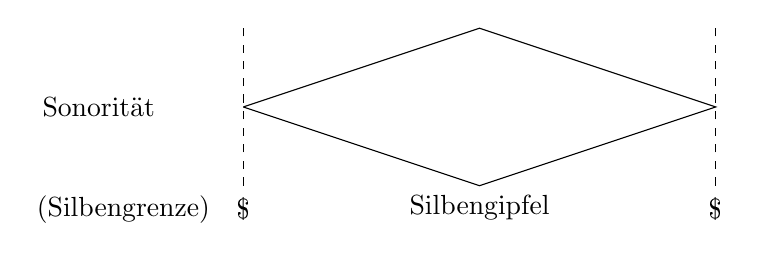
\begin{tikzpicture}
	\draw[dashed] (-3,0)--(-3,2);
	\draw[dashed] (3,0)--(3,2);
	\draw[black] (-3,1)--(0,2)--(3,1)--(0,0)--(-3,1);
	\node at (-3,-0.3){\$};
	\node at (3,-0.3){\$};
	\node[left] at (-3.3,-0.3){(Silbengrenze)};
	\node[left] at (-4,1){Sonorität};
	\node[below] at (0,0){Silbengipfel};
	\end{tikzpicture}
	\caption{Sonoritätsskala in \citet[19]{Lenerz85a}} %\citet[93]{Ramers08a}
\end{figure}
% Vokale sind sonorste Elemente
% m > p
% s > p  (frikativ > plosiv)

\begin{itemize}
	\item Laute können nach der Sonoritätshierarchie auf einer Skala (nach ihrer \textbf{Sonorität}) angeordnet werden.
\end{itemize}

\end{frame}


%%%%%%%%%%%%%%%%%%%%%%%%%%%%%%%%%%
\begin{frame}
\frametitle{Varianten der Sonoritätshierarchie}

Es gibt verschiedene Ausformulierungen der Sonoritätshierachie.


\begin{table}
\centering
\begin{tabular}{l|l|l|l|l} 
	 & einfach 				  	 & Hall 					  & \textbf{Wiese} 				& komplex  \\ 
\hline
\hline 
$[+]$& \multirow{6}{*}{Sonorant} & \multirow{2}{*}{Vokal} 	  & \multirow{2}{*}{Vokal} 		& Vokal  \\ 
	 & 							 & 						 	  &								& Vokal (hoch) \\
\cline{3-5}			
	 &							 & \multirow{3}{*}{Liquide}   &								& Gleitlaut \\
	 &						  	 &	 						  & \textipa{/\textscr /}		& Vibrant \\
\cline{4-5}			
	 &						 	 &							  & \textipa{/l/}				& Lateral \\
\cline{3-5}			
	 &							 & Nasal					  & Nasal						& Nasal \\
\hline			
	 &\multirow{6}{*}{Obstruent} & \multirow{6}{*}{Obstruent} & \multirow{3}{*}{Frikativ}	& $[+$sth$]$ Frikativ \\
	 &						 	 &							  &								& $[+$sth$]$ Affrikat \\		
	 &							 &							  &								& $[+$sth$]$ Plosiv \\
\cline{4-5}			
	 &						  	 &							  & \multirow{3}{*}{Plosiv}		& $[-$sth$]$ Frikativ \\
	 &						 	 &							  &								& $[-$sth$]$ Affrikat \\		
$[-]$&							 &							  &								& $[-$sth$]$ Plosiv \\
		
\end{tabular} 

\end{table}

\end{frame}



%%%%%%%%%%%%%%%%%%%%%%%%%%%%%%%%%%

\begin{frame}
%\frametitle{Sonoritätshierarchie}


\begin{block}{Sonoritätsprinzip (Sonority Sequencing Generalization -- SSG)}
In jeder Silbe gibt es ein Segment, das den \textbf{Silbengipfel} bildet, und dem ein oder mehrere Segmente vorangehen und/oder folgen, deren Sonoritätswerte \textbf{zum Silbengipfel hin zunehmen} und \textbf{danach abnehmen}.\\
\hfill (vgl. \citealt[225]{Hall00a}, \citealt[94]{Ramers08a})
\end{block}

\begin{itemize}
	\item Strikt: monoton steigend oder fallend
	\item Abgeschwächt: auch gleichbleibend \citep[vgl.][]{Hall00a}

\end{itemize}


\begin{figure}
	\centering
	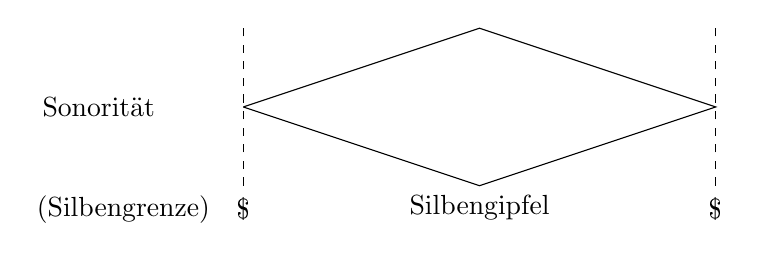
\begin{tikzpicture}
	\draw[dashed] (-3,0)--(-3,2);
	\draw[dashed] (3,0)--(3,2);
	\draw[black] (-3,1)--(0,2)--(3,1)--(0,0)--(-3,1);
	\node at (-3,-0.3){\$};
	\node at (3,-0.3){\$};
	\node[left] at (-3.3,-0.3){(Silbengrenze)};
	\node[left] at (-4,1){Sonorität};
	\node[below] at (0,0){Silbengipfel};
\end{tikzpicture}
	\caption{Sonoritätsskala in \citet[19]{Lenerz85a}} %\citet[93]{Ramers08a}
\end{figure}


\end{frame}


%%%%%%%%%%%%%%%%%%%%%%%%%%%%%%%%%%
\begin{frame}
%\frametitle{Sonoritätshierarchie}

\begin{block}{Sonoritätshierarchie (für uns)}
Vokal $>$ \textipa{/\textscr /} $>$ \textipa{/l/} $>$ Nasal $>$ Frikativ $>$ Plosiv \\
$x > y$ $:=$ $x$ ist sonorer als $y$
\end{block}

\begin{figure}
	\centering
	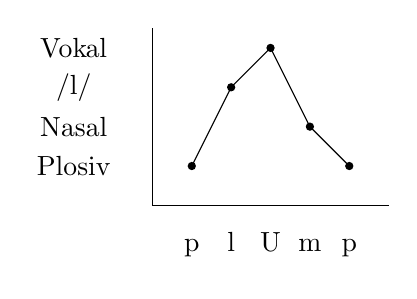
\begin{tikzpicture}[scale=0.5]
	\draw[black] (-1,0) -- (5,0) ; % x axis
	\draw[black] (-1,0) -- (-1,4.5); % y axis
	\node at (-3,1) {Plosiv};
	\node at (-3,2) {Nasal};
	\node at (-3,3) {\textipa{/l/}};
	\node at (-3,4) {Vokal};
	\draw[black] (0,1) -- (1,3) -- (2,4) -- (3,2) -- (4,1);
	\node at (0,-1) {\strut \textipa{p}};
	\node at (1,-1) {\strut \textipa{l}};
	\node at (2,-1) {\strut \textipa{U}};
	\node at (3,-1) {\strut \textipa{m}};
	\node at (4,-1) {\strut \textipa{p}};
	\fill (0,1) circle [radius=3pt];
	\fill (1,3) circle [radius=3pt];
	\fill (2,4) circle [radius=3pt];
	\fill (3,2) circle [radius=3pt];
	\fill (4,1) circle [radius=3pt];
	\end{tikzpicture}
\caption{\citep[225]{Hall00a}}
\end{figure}


%\begin{figure}
%\centering
%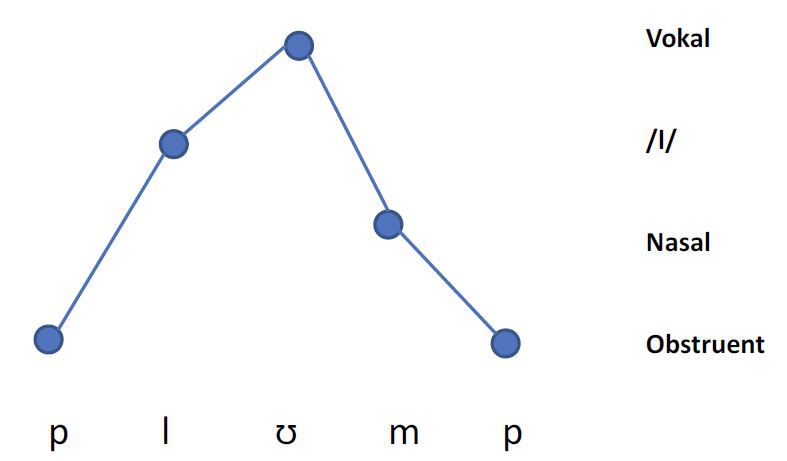
\includegraphics[scale=.3]{material/03bSonoritaetBsp}
%\caption{\citet[225]{Hall00a}}
%\end{figure}

\begin{itemize}
	\item Sonoritätshierarchie wird je nach Sprache leicht anders spezifiziert.
\end{itemize}
\end{frame}


%%%%%%%%%%%%%%%%%%%%%%%%%%%%%%%%%%
\begin{frame}
\frametitle{Übung}

\begin{itemize}
	\item Geben Sie die Sonoritätsprofile der folgenden Silben an.
	
	\ea Spatz, Dachs, Clown, Milch
	\z
	
	% bei Spatz geht es von Frikativ s auf Plosiv p runter = Ausnahme
	% bei Dachs geht es auf k runter und dann auf s hoch   = Ausnahme
	% clown k = plosiv, l = /l/ au = Vokal, n = , keine Ausnahme
	
	% Glottal stop gehört zu den Plosiven
	
	\item Erklären Sie die Ungrammatikalität der folgenden Silben:
	
	\begin{exe}
	\ex \label{ex:lbat}
	\begin{xlist}
		\ex [*]{\textipa{[lbat]}}
		\ex [*]{\textipa{[blabl]}}
		\ex [*]{\textipa{[ki:l\textscr]}}
		\ex [*]{\textipa{[ngang]}}
		\ex [*]{\textipa{[krafm]}}
		\ex [*]{\textipa{[elat]}}
		\ex [*]{\textipa{[plaml]}}
		\ex [*]{\textipa{[nfatl]}}
	\end{xlist}
\end{exe}
	
\end{itemize}

\end{frame}


%%%%%%%%%%%%%%%%%%%%%%%%%%%%%%%%%%%
\iftoggle{ue-loesung}{
	%%%%%%%%%%%%%%%%%%%%%%%%%%%%%%%%%%
%% UE 1 - 03b Phonologie
%%%%%%%%%%%%%%%%%%%%%%%%%%%%%%%%%%

\begin{frame}
\frametitle{Übung: Sonoritätsprofile -- Lösung}

\vfill
\hfill
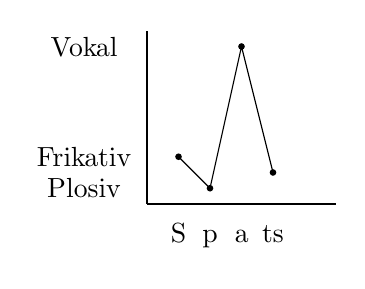
\begin{tikzpicture}[scale=0.4]
\draw[black] (-1,0) -- (5,0) ; % x axis
\draw[black] (-1,0) -- (-1,5.5); % y axis
\node at (-3,0.5) {Plosiv};
\node at (-3,1.5) {Frikativ};
\node at (-3,5) {Vokal};
\draw[black] (0,1.5) -- (1,0.5) -- (2,5) -- (3,1);
\node at (0,-1) {\strut \textipa{S}};
\node at (1,-1) {\strut \textipa{p}};
\node at (2,-1) {\strut \textipa{a}};
\node at (3,-1) {\strut \textipa{\texttoptiebar{ts}}};
\fill (0,1.5) circle [radius=3pt];
\fill (1,0.5) circle [radius=3pt];
\fill (2,5) circle [radius=3pt];
\fill (3,1) circle [radius=3pt];
\end{tikzpicture}
\pause
\hfill
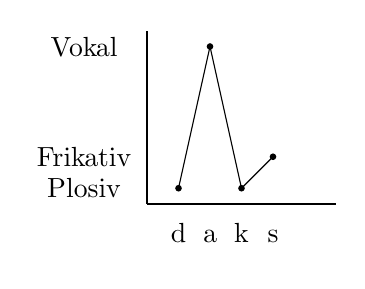
\begin{tikzpicture}[scale=0.4]
\draw[black] (-1,0) -- (5,0) ; % x axis
\draw[black] (-1,0) -- (-1,5.5); % y axis
\node at (-3,0.5) {Plosiv};
\node at (-3,1.5) {Frikativ};
\node at (-3,5) {Vokal};
\draw[black] (0,0.5) -- (1,5) -- (2,0.5) -- (3,1.5);
\node at (0,-1) {\strut \textipa{d}};
\node at (1,-1) {\strut \textipa{a}};
\node at (2,-1) {\strut \textipa{k}};
\node at (3,-1) {\strut \textipa{s}};
\fill (0,0.5) circle [radius=3pt];
\fill (1,5) circle [radius=3pt];
\fill (2,0.5) circle [radius=3pt];
\fill (3,1.5) circle [radius=3pt];
\end{tikzpicture}
\hfill\mbox{}
\vfill
\pause
\hfill
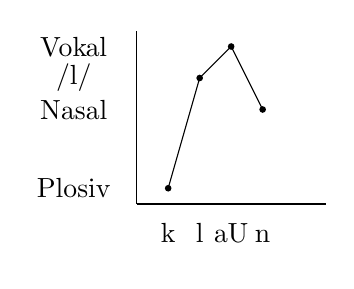
\begin{tikzpicture}[scale=0.4]
\draw[black] (-1,0) -- (5,0) ; % x axis
\draw[black] (-1,0) -- (-1,5.5); % y axis
\node at (-3,0.5) {Plosiv};
\node at (-3,3) {Nasal};
\node at (-3,4) {\textipa{/l/}};
\node at (-3,5) {Vokal};
\draw[black] (0,0.5) -- (1,4) -- (2,5) -- (3,3);
\node at (0,-1) {\strut \textipa{k}};
\node at (1,-1) {\strut \textipa{l}};
\node at (2,-1) {\strut \textipa{\texttoptiebar{aU}}};
\node at (3,-1) {\strut \textipa{n}};
\fill (0,0.5) circle [radius=3pt];
\fill (1,4) circle [radius=3pt];
\fill (2,5) circle [radius=3pt];
\fill (3,3) circle [radius=3pt];
\end{tikzpicture}
\hfill
\pause
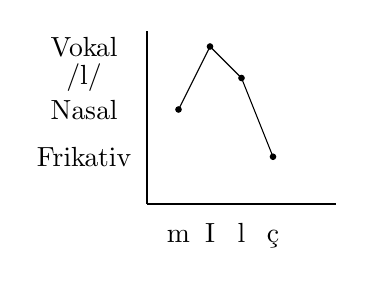
\begin{tikzpicture}[scale=0.4]
\draw[black] (-1,0) -- (5,0) ; % x axis
\draw[black] (-1,0) -- (-1,5.5); % y axis
\node at (-3,1.5) {Frikativ};
\node at (-3,3) {Nasal};
\node at (-3,4) {\textipa{/l/}};
\node at (-3,5) {Vokal};
\draw[black] (0,3) -- (1,5) -- (2,4) -- (3,1.5);
\node at (0,-1) {\strut \textipa{m}};
\node at (1,-1) {\strut \textipa{I}};
\node at (2,-1) {\strut \textipa{l}};
\node at (3,-1) {\strut \textipa{\c{c}}};
\fill (0,3) circle [radius=3pt];
\fill (1,5) circle [radius=3pt];
\fill (2,4) circle [radius=3pt];
\fill (3,1.5) circle [radius=3pt];
\end{tikzpicture}
\hfill\mbox{}
\vfill
\end{frame}


%%%%%%%%%%%%%%%%%%%%%%%%%%%%%%%%%%
\begin{frame}
\frametitle{Übung -- Lösung}

\begin{itemize}
\item Erklären Sie die Ungrammatikalität der folgenden Silben:\\
(Vokal $>$ \textipa{/\textscr /} $>$ \textipa{/l/} $>$ Nasal $>$ Frikativ $>$ Plosiv)
\begin{exe}
	\exr{ex:lbat}
	\settowidth\jamwidth{XXXXXXXXXXXXXXXXXXXXXXXXXXXXXXXXXX}
	\begin{xlist}
		\ex[*]{ \textipa{[lbat]}\loesung{2}{\textipa{[l]} vor \textipa{[b]} im Onset} }
		\ex[*]{ \textipa{[blabl]}\loesung{3}{\textipa{[b]} vor \textipa{[l]} in der Koda $+$ Auslautverhärtung} }
		\ex[*]{ \textipa{[ki:l\textscr]}\loesung{5}{\textipa{[l]} vor \textipa{[\textscr ]} in der Koda} }
		\ex[*]{ \textipa{[ngang]}\loesung{6}{\textipa{[n]} vor \textipa{[g]} im Onset $+$ reg. velare Nasalassimiliation } \loesung{6}{$+$ g-Tilgung}}
		\ex[*]{ \textipa{[krafm]}\loesung{7}{\textipa{[f]} vor \textipa{[m]} in der Koda} }
		\ex[*]{ \textipa{[elat]}\loesung{8}{2 Silben (2 Nuklei) $+$ Knacklauteinsetzung} }
		\ex[*]{ \textipa{[plaml]}\loesung{9}{\textipa{[m]} vor \textipa{[l]} in der Koda} }
		\ex[*]{ \textipa{[nfatl]}\loesung{10}{\textipa{[n]} vor \textipa{[f]} im Onset $+$ \textipa{[t]} vor \textipa{[l]} in der Koda} }
	\end{xlist}
\end{exe}

\end{itemize}

\end{frame}


}
%%%%%%%%%%%%%%%%%%%%%%%%%%%%%%%%%%

\subsubsection{Weitere phonotaktische Beschränkungen}

%%%%%%%%%%%%%%%%%%%%%%%%%%%%%%%%%%

\begin{frame}
\frametitle{Weitere phonotaktische Beschränkungen}

\begin{columns}
	
	\column{.6\textwidth}	
\begin{itemize}
	\item Im \textbf{Onset} in deutschen Silben können stehen:
	
	\begin{itemize}
		\item alle Einzelkonsonanten des Deutschen 
		
		(\textbf{außer} \textipa{[N]} und \textipa{[s]} vor Vokal am Wortanfang)

		\item bestimmte zwei- und dreigliedrige Konsonantencluster nach Sonoritätshierarchie
		
		\item bestimmte zweigliedrige Konsonantencluster\\
		 (s. Tabelle: von links nach oben im Onset, in der Koda umgekehrt, \citealp[vgl.][231-235]{Hall00a})
	\end{itemize}

	\ea *\textipa{[fma]} \vs \textipa{[fla]}
	\ex *\textipa{[lpa]} \vs \textipa{[pla]}
	\ex *\textipa{[mSa]} \vs \textipa{[Sma]}
	\ex *\textipa{[m\;Ra]}
	\z
\end{itemize}
	
	\column{.35\textwidth}
\begin{table}
	\centering
	
	\begin{tabular}{c|c|c|c|c}
		& \textipa{m} & \textipa{n} & \textipa{l} & \textipa{\textscr} \\ 
		\hline 
		\textipa{p} &  &  & $+$ & $+$ \\ 
		\hline 
		\textipa{b} &  &  & $+$ & $+$ \\ 
		\hline 
		\textipa{t} &  &  &  & $+$ \\ 
		\hline 
		\textipa{d} &  &  &  & $+$ \\ 
		\hline 
		\textipa{k} &  & $+$ & $+$ & $+$ \\ 
		\hline 
		\textipa{g} &  & $+$ & $+$ & $+$ \\ 
		\hline 
		\textipa{f} &  &  & $+$ & $+$ \\
		\hline 
		\textipa{v} &  &  &  & $+$ \\ 
		\hline 
		\textipa{S} & $+$ & $+$ & $+$ & $+$ \\ 
	\end{tabular} 
	
	\caption{Kombinatorik von Sonoranten mit Obstruenten im Deutschen}
\end{table}

\end{columns}	

\end{frame}	
%%%%%%%%%%%%%%%%%%%%%%%%%%%%%%%%%

\begin{frame}{Weitere phonotaktische Beschränkungen}
	
\begin{itemize}	
	\item Silben können auch \textbf{mit unbetontem Vokal} beginnen (\ras leerer Onset).
	\ea \ab{Eier}: \textipa{[\textprimstress P\t{aɪ}.\alertred{5}]}
	\z
	
	\ea \ab{etwaig}: \textipa{[PEt.\textprimstress va:.\alertred{I}\c{c}]} 
	\z

\pause 
	
	\item Vor betontem Vokal steht immer ein Konsonant (\textbf{Glottisschlag}).
	
	\ea
	\textipa{[ka.\alertred{\textprimstress Po:}.tIS]}
	\z

\end{itemize}

\end{frame}


%%%%%%%%%%%%%%%%%%%%%%%%%%%%%%%%%%
\subsection{Hausaufgabe}
%%%%%%%%%%%%%%%%%%%%%%%%%%%%%%%%%%

\begin{frame}
\frametitle{Hausaufgabe}

\begin{itemize}
	\item[1.]{Geben Sie die standarddeutsche \textbf{phonetische Transkription} für folgende Wörter an:}
	
	\eal \label{ex:03bHA1}
	\ex Spitzenschuhe
	\ex Endausscheidung
	\ex Platzanweiser
	\ex verzweifeln
	\ex abverlangen
	\ex Überarbeitung
	\ex Zugeständnis
	\zl
\end{itemize}

\end{frame}
%%%%%%%%%%%%%%%%%%%%%%%%%%%%%%%%%

\begin{frame}{Hausaufgabe}

\begin{itemize}
\item[2.]{Erläutern Sie anhand der folgenden Beispiele, unter welchen Bedingungen die \textbf{Auslautverhärtung} im Deutschen stattfindet.}

\eal \label{ex:03bHA2}
\ex Wand -- Wände
\ex lesen -- lesbar
\ex sagen -- sagst
\ex Roggen
\zl

\end{itemize}

\end{frame}
%%%%%%%%%%%%%%%%%%%%%%%%%%%%%%%%%%

\begin{frame}{Hausaufgabe}

\begin{itemize}
\item[3.]{Geben Sie fünf verschiedene \textbf{phonetische oder phonologische Prozesse} an, die in dem folgenden Satz -- teilweise nur bei schnellerem Sprechen -- beobachtet werden können.} 

\ea \label{ex:03bHA3}
\begin{quote}
Um die fünf Haken in regelmäßigen Abständen an die Wand schrauben zu können, sollten Sie sich Bohrmaschine, Wasserwaage, Zollstock und Dübel bereitgelegt haben und auf keinen Fall die Nerven verlieren, bevor Sie nicht befestigt sind.
\end{quote}
\z

\end{itemize}

\end{frame}
%%%%%%%%%%%%%%%%%%%%%%%%%%%%%%%%%%%

\begin{frame}{Hausaufgabe}

\begin{itemize}	
\item[4.]{Illustrieren Sie den deutschen phonemischen Kontrast der folgenden Phoneme durch
  \textbf{Minimalpaare}, wobei der Kontrast (wenn möglich) ein Mal initial,\\
ein Mal final vorkommen soll.

Beispiel: \textipa{[p]} -- \textipa{[f]} Paul -- faul (Initialposition), Laub -- Lauf (Finalposition)}

\eal \label{ex:03bHA4}
\ex \textipa{[m]} -- \textipa{[n]}
\ex \textipa{[p]} -- \textipa{[b]}
\ex \textipa{[h]} -- \textipa{[v]}
\ex \textipa{[n]} -- \textipa{[N]}
\ex \textipa{[f]} -- \textipa{[v]}
\zl

\end{itemize}
\end{frame}


%%%%%%%%%%%%%%%%%%%%%%%%%%%%%%%%%%%
\iftoggle{ha-loesung}{
	%%%%%%%%%%%%%%%%%%%%%%%%%%%%%%%%%%
%% HA 1 - 03b Phonologie
%%%%%%%%%%%%%%%%%%%%%%%%%%%%%%%%%%

\begin{frame}
\frametitle{Hausaufgabe -- Lösung}

\begin{itemize}
	\item[1.]{Geben Sie die standarddeutsche \textbf{phonetische Transkription} für folgende Wörter an:}
	
	\begin{exe}
		\exr{ex:03bHA1}
		\begin{xlist}
		\settowidth\jamwidth{XXXXXXXXXXXXXXXXXXXXXXXXXXXXXX}
			\ex Spitzenschuhe \loesung{2}{\textipa{['SpI\textsubdot{\t{ts}}@n.Su:.@]}}
			\ex Endausscheidung \loesung{3}{\textipa{['PEnt.P\texttoptiebar{aU}s.S\texttoptiebar{aI}.dUN]}}
			\ex Platzanweiser \loesung{4}{\textipa{['pla\texttoptiebar{ts}.Pan.v\texttoptiebar{aI}.z5]}}
			\ex verzweifeln \loesung{5}{\textipa{[fE5.'\texttoptiebar{ts}v\texttoptiebar{aI}.f@ln]}}
			\ex abverlangen \loesung{6}{\textipa{['Pap.fE5.la\.N@n]}}
			\ex Überarbeitung \loesung{7}{\textipa{[Py:.b5.'Pa\;R.b\texttoptiebar{aI}.tUN]}}
			\ex Zugeständnis \loesung{8}{\textipa{['\texttoptiebar{ts}u:.g@.StEnt.nIs]}}
		\end{xlist}
	\end{exe}

\end{itemize}

\end{frame}
%%%%%%%%%%%%%%%%%%%%%%%%%%%%%%%%%

\begin{frame}{Hausaufgabe -- Lösung}

\begin{itemize}
	\item[2.]{Erläutern Sie anhand der folgenden Beispiele, unter welchen Bedingungen die \textbf{Auslautverhärtung} im Deutschen stattfindet.}

	\begin{exe}
		\exr{ex:03bHA2}
		\begin{xlist}
		\settowidth\jamwidth{XXXXXXXXXXXXXXXXXXXXXXXXXXXXXXX}
			\ex Wand -- Wände \loesung{2}{sth. Plosive am Wortende}
			\ex lesen -- lesbar \loesung{3}{generell am Silbenende}
			\ex sagen -- sagst \loesung{4}{betrifft \emph{alle} sth. Plosive in der Koda}
			\ex Roggen \loesung{5}{jedoch keine Silbengelenke}
		\end{xlist}
	\end{exe}

\end{itemize}

\end{frame}


%%%%%%%%%%%%%%%%%%%%%%%%%%%%%%%%%%
\begin{frame}{Hausaufgabe -- Lösung}

\begin{itemize}
\item[3.]{Geben Sie fünf verschiedene \textbf{phonetische oder phonologische Prozesse} an, die in dem folgenden Satz -- teilweise nur bei schnellerem Sprechen -- beobachtet werden können.} 

\begin{exe}
	\exr{ex:03bHA3}
	\begin{quote}
	Um die fünf Haken in regelmäßigen Abständen an die Wand schrauben zu können, sollten Sie sich Bohrmaschine, Wasserwaage, Zollstock und Dübel bereitgelegt haben und auf keinen Fall die Nerven verlieren, bevor Sie nicht befestigt sind.
	\end{quote}
\end{exe}


\begin{description}
	\item[\alertgreen{\textbf{Beispiele:}}] ~

\alertgreen{
	regressive Nasalassimilation in \emph{fünf}: \textipa{[fY\textbf{m}f]}\\
	progressive Nasalassimilation nach Schwa-Elision (feeding) in \emph{Haken}: \textipa{[hak\textbf{N}]}\\
	Auslautverhärtung in \emph{Wand}: \textipa{[van\textbf{t}]}\\
	progressive Nasalassimilation nach Schwa-Elision (feeding) in \emph{schrauben}: \textipa{[S\;R\t{aU}b\textbf{m}]}\\
	g-Spirantisierung in \emph{befestigt}: \textipa{[b@fEstI\textbf{\c{c}}t]}\\
	r-Vokalisierung in \emph{Bohrmaschine}: \textipa{[bo\textbf{5}maSi:n@]}
}						
		\end{description}

\end{itemize}

\end{frame}


%%%%%%%%%%%%%%%%%%%%%%%%%%%%%%%%%%%
\begin{frame}{Hausaufgabe -- Lösung}

\begin{itemize}	
\item[4.]{Illustrieren Sie den deutschen phonemischen Kontrast der folgenden Phoneme durch \textbf{Minimalpaare}, wobei der Kontrast (wenn möglich) ein Mal initial,\\ ein Mal final vorkommen soll.

Beispiel: \textipa{[p]} -- \textipa{[f]} Paul -- faul (Initialposition), Laub -- Lauf (Finalposition)}

\begin{exe}
	\exr{ex:03bHA4}
	\settowidth\jamwidth{XXXXXXXXXXXXXXXXXXXXXXXXXXXXXXXXXXXX}
	\begin{xlist}
		\ex \textipa{[m]} -- \textipa{[n]} \loesung{2}{muss -- Nuss, beim -- Bein}
		\ex \textipa{[p]} -- \textipa{[b]} \loesung{3}{Pass -- Bass}
			\loesung{3}{(wegen Auslautverhärtung kein finaler Kontrast möglich)}
		\ex \textipa{[h]} -- \textipa{[v]} \loesung{4}{heiß -- weiß (\textipa{[h]} kommt nicht final vor)}
		\ex \textipa{[n]} -- \textipa{[N]} \loesung{5}{Sinn -- sing (\textipa{[N]} kommt nicht initial vor)}
		\ex \textipa{[f]} -- \textipa{[v]} \loesung{6}{Fass -- was}
			\loesung{6}{(wegen Auslautverhärtung kein finaler Kontrast möglich)}
	\end{xlist}
\end{exe}
		
\end{itemize}

\end{frame}

}
%%%%%%%%%%%%%%%%%%%%%%%%%%%%%




%@EE: Checken: Keine Abbildungen und elektronischen Quellen?


%%%%%%%%%%%%%%%%%%%%%%%%%%%%%%%%%%%%%%%%%%%%%%%%
%% Compile the master file!
%% 		Include: Antonio Machicao y Priemer
%% 		Course: GK Linguistik
%%%%%%%%%%%%%%%%%%%%%%%%%%%%%%%%%%%%%%%%%%%%%%%%

%\exewidth{(35)} im übergeordneten File

% sollte zentral geladen werden. St. Mü. 04.11.2016 (in localcommands?)
%%%%%%%%%%%%%
%%% Forestset Syllables

\newbox\foreststrutbox
\setbox\foreststrutbox=\hbox to 0pt{\phantom{\forestOve{standard node}{content}}}
\def\foreststrut{\copy\foreststrutbox}
\forestset{
GP1/.style 2 args={
for n={1}{baseline},
s sep=0pt, l sep=0pt,
for descendants={
l sep=0pt, l={#1},
anchor=base,calign=first,child anchor=north,
inner xsep=1pt,inner ysep=2pt,outer sep=0pt,s sep=0pt,
},
delay={
if content={}{phantom}{for children={no edge}},
for tree={
if content={O}{tier=OR}{},
if content={R}{tier=OR}{},
if content={N}{tier=N}{},
if content={x}{
tier=x,content={$\times$},outer xsep={#2},
for tree={calign=center},
for descendants={content format={\foreststrut\forestoption{content}}},
before drawing tree={outer xsep=0pt,delay={typeset node}},
s sep=4pt
}{},
},
},
before drawing tree={where content={}{parent anchor=center,child anchor=center}{}},
},
GP1/.default={5ex}{8.0pt},
associate/.style={%
tikz+={\draw(!)--(!#1);}},
spread/.style={
before drawing tree={tikz+={\draw[dotted](!)--(!#1);}}},
govern/.style={
before drawing tree={tikz+={\draw[->](!)--(!#1);}}},
p-govern/.style={
before drawing tree={tikz+={\draw[->](.north) to[out=150,in=30] (!#1.north);}}},
no p-govern/.style={
before drawing tree={tikz+={\draw[->,loosely dashed](.north) to[out=150,in=30] (!#1.north);}}},
encircle/.style={before drawing tree={circle,draw,inner sep=0pt}},
fen/.style={pin={[font=\footnotesize,inner sep=1pt,pin edge=<-]10:\textsc{Fen}}},
el/.style={content=\textsc{\textbf{##1}}},
head/.style={content=\textsc{\textbf{\underline{##1}}}},
llap/.style={
tikz+={%
\edef\forest@temp{\noexpand\node[\option{node options},
anchor=base east,at=(.base east)]}%
\forest@temp{#1\phantom{\option{environment}}};
}
},
rlap/.style={
tikz+={%
\edef\forest@temp{\noexpand\node[\option{node options},
anchor=base west,at=(.base west)]}%
\forest@temp{\phantom{\option{environment}}#1};
}
},
}
%%%%%%%%%%%%%


%%%%%%%%%%%%%%%%%%%%%%%%%%%%%%%%%%%%%%%%%%%%%%%%%%%%
%%%             Metadata                         
%%%%%%%%%%%%%%%%%%%%%%%%%%%%%%%%%%%%%%%%%%%%%%%%%%%% 

\title{Grundkurs Linguistik}

\subtitle{Phonologie III: Silbenmodelle}

\author[A. Machicao y Priemer]{
	{\small Antonio Machicao y Priemer}
	\\
	{\footnotesize \url{http://www.linguistik.hu-berlin.de/staff/amyp}}
	%	\\
	%	{\small\href{mailto:mapriema@hu-berlin.de}{mapriema@hu-berlin.de}}
}

\institute{Institut für deutsche Sprache und Linguistik}

% bitte lassen, sonst kann man nicht sehen, von wann die PDF-Datei ist.
%\date{ }

%\publishers{\textbf{6. linguistischer Methodenworkshop \\ Humboldt-Universität zu Berlin}}

%\hyphenation{nobreak}


%%%%%%%%%%%%%%%%%%%%%%%%%%%%%%%%%%%%%%%%%%%%%%%%%%%%
%%%             Preamble's End                  
%%%%%%%%%%%%%%%%%%%%%%%%%%%%%%%%%%%%%%%%%%%%%%%%%%%%   


%%%%%%%%%%%%%%%%%%%%%%%%%   
\huberlintitlepage[22pt]
\iftoggle{toc}{
\frame{
%\begin{multicols}{2}
	\frametitle{Inhaltsverzeichnis}
	\tableofcontents
	%[pausesections]
%\end{multicols}
}
}

%%%%%%%%%%%%%%%%%%%%%%%%%%%%%%%%%%
%%%%%%%%%%%%%%%%%%%%%%%%%%%%%%%%%%
%%%%%LITERATURE:

%% Allgemein
\nocite{Glueck&Roedel16a}
\nocite{Schierholz&Co18}
\nocite{Luedeling2009a}
\nocite{Meibauer&Co07a} 
\nocite{Repp&Co15a} 

%%% Sprache & Sprachwissenschaft
%\nocite{Fries16c} %Adäquatheit
%\nocite{Fries16a} %Grammatikalität
%\nocite{Fries&MyP16c} %GG
%\nocite{Fries&MyP16b} %Akzeptabilität
%\nocite{Fries&MyP16d} %Kompetenz vs. Performanz

%% Phonetik & Phonologie
\nocite{Altmann&Co07a}
\nocite{DudenAussprache00a}
\nocite{Hall00a} 
\nocite{Kohler99a}
\nocite{Krech&Co09a}
\nocite{Pompino95a}
\nocite{Ramers08a}
\nocite{Ramers&Vater92a}
\nocite{Rues&Co07a}
\nocite{WieseR96a}
\nocite{WieseR11a}


%%%%%%%%%%%%%%%%%%%%%%%%%%%%%%%%%%
%%%%%%%%%%%%%%%%%%%%%%%%%%%%%%%%%%
\section{Phonologie III: Silbenmodelle}
%%%%%%%%%%%%%%%%%%%%%%%%%%%%%%%%%%
\begin{frame}
\frametitle{Begleitlektüre}

\begin{itemize}
	\item \textbf{obligatorisch:}
	\begin{itemize}
		\item[] AM S.~24--30
		\item[] \citet{Hall00a}: Kapitel~2 (S.~47--62)
	\end{itemize}
	\item \textbf{optional:}
	\begin{itemize}
		\item[] \citet{Hall00a}: Kapitel~8 (S.~238--254)
	\end{itemize}
\end{itemize}

\end{frame}


%%%%%%%%%%%%%%%%%%%%%%%%%%%%%%%%%%
%%%%%%%%%%%%%%%%%%%%%%%%%%%%%%%%%%
\subsection{Silbenmodelle}

%% MyP: Contents
\iftoggle{sectoc}{
	\frame{
		%\begin{multicols}{2}
		\frametitle{~}
		\tableofcontents[currentsubsection, subsubsectionstyle=hide]
		%\end{multicols}
	}
}

%% StM: Contents
\iftoggle{gliederung}{
	
	\outline{
		\begin{itemize}
			
			\item \blaubf{Silbenmodelle}
			%% CV-Modell
			%% Konstituentenmodell
			\item Silbengelenk
			\item Silbifizierung
			\item Exkurs: Akzent
			\item Hausaufgabe
			
		\end{itemize}
	}
}
%%%%%%%%%%%%%%%%%%%%%%%%%%%%%%%%%%

\begin{frame}
\frametitle{Silbenmodelle}

\begin{itemize}
	\item Bisher (hauptsächlich) nur \textbf{lineare Betrachtung} mit allen Segmenten auf einer Schicht
	\ea
	\textipa{/pe:.t@\textscr /} (Peter)
	\z
	
	\ea
	\textipa{/vE\.t@\textscr /} (Vetter)
	\z
	
	\item \textbf{Nicht-lineare Phonologie} (Autosegmentale Phonologie)
	
	\begin{itemize}
		\item verschiedene Repräsentationsebenen bzw. Schichten
		
		\item hierarchische Strukturierung
		
		\item Vorteil: 
		
		Beschreibung von \textbf{Merkmalsausbreitung} und \textbf{segmentunabhängigen Prozessen}
		
	\end{itemize}
\end{itemize}

\end{frame}


%%%%%%%%%%%%%%%%%%%%%%%%%%%%%%%%%%
%%%%%%%%%%%%%%%%%%%%%%%%%%%%%%%%%%
\subsubsection{CV-Modell}
%\frame{
%\frametitle{~}
%	\tableofcontents[currentsection]
%}
%%%%%%%%%%%%%%%%%%%%%%%%%%%%%%%%%%

\begin{frame}%[shrink]
\frametitle{CV-Modell (einfaches Modell)}

\begin{itemize}
\item Silben und Segmente auf unterschiedlichen Schichten

\item verbunden durch Assoziationslinien

\item Charakterisierung der Silbenstruktur durch C und V 
\end{itemize}

\begin{columns}
	
\column[c]{.45\textwidth}
\begin{figure}
	\centering
	\begin{forest}
		MyP edges,
		[$\sigma$
		[C [\textipa{b}]]
		[C [\textipa{l}]]
		[V [\textipa{I}]]
		[C [\textipa{n}]]
		[C [\textipa{t}]]
		]
	\end{forest}
	\caption{CV-Modell}
\end{figure}


\column[c]{.5\textwidth}
$\sigma :=$ Silbe

C $:=$ nicht-silbisch, \gqq{konsonantisch}

V $:=$ silbisch, \gqq{vokalisch}

\end{columns}

\end{frame}


%%%%%%%%%%%%%%%%%%%%%%%%%%%%%%%%%%
\begin{frame}
\frametitle{Verteilung von Segmenten in der Silbe}

\begin{itemize}
\item Wie ist die Verteilung von Segmenten in der deutschen Silbe?
\end{itemize}

\begin{minipage}{.59\textwidth}
	\begin{itemize}
	\item C $\neq$ Konsonant, sondern \alertred{nicht-silbisch}
	
	\item V $\neq$ Vokal, sondern \alertblue{silbisch}
	
	\item Jede Silbe enthält \alertgreen{einen Kern} (V).
	\end{itemize}
\end{minipage}
%
\begin{minipage}{.4\textwidth}

\begin{figure}
%\tiny
\small
\centering
\begin{forest}
	MyP edges,
	[$\sigma$
	[C [\textipa{g}]]
	[C [\textipa{l}]]
	[\alertgreen{V} [\textipa{a}]]	
	[C [\alertred{\textipa{U}}]]
	[C [\textipa{p}]]
	[C [\textipa{t}]]
	]
\end{forest}

\begin{forest}
	MyP edges,
	[,phantom
	[$\sigma$
	[C [\textipa{k}]]
	[\alertgreen{V} [\textipa{U}]]
	[C [\textipa{m}]]
	]
	[$\sigma$	
	[C [\textipa{p}]]
	[\alertgreen{V} [\alertblue{\textipa{\textsyllabic{l}}}]]
	]
	]
\end{forest}

\end{figure}

\end{minipage}

% u bei glaubt ist ein C, weil nur a der Silbengipfel ist, u ist weniger sonor, und Diphtonge gelten
% als zwei Zeiteinheiten, bei langen Vokalen wird auch auf zwei geteilt. Der Doppelpunkt ist dann
% ein C

% Bei Beirisch guot geht der Sonoritätsgipfel aufs o und dann ist das o V und davor ein C

\end{frame}


%%%%%%%%%%%%%%%%%%%%%%%%%%%%%%%%%%
\begin{frame}
\frametitle{Verteilung von Segmenten in der Silbe}


\begin{minipage}{.59\textwidth}
	\begin{itemize}
	\item \textbf{maximale Anzahl an Cs} vor und nach V
	
	% Aber strumpfst. Es kommt ein weiteres verbessertes Modell
	
	\item Korrelation zwischen Anzahl an Cs nach V und der \textbf{Länge}/(Un-)Gespanntheit des
          Vokals:\\
              normalerweise nach Lnagvokal kein Konsonantencluster
	\end{itemize}
\end{minipage}
%
\begin{minipage}{.4\textwidth}

\begin{figure}
	%\tiny
	\small
	\centering
	\begin{forest}
	MyP edges,
	[$\sigma$
	[C [\textipa{g}]]
	[C [\textipa{l}]]
	[V [\textipa{a}]]	
	[\alertred{C} [\textipa{U}]]
	[\alertred{C} [\textipa{p}]]
	[\alertred{C} [\textipa{t}]]
	]
	\end{forest}
	
	\begin{forest}
	MyP edges,
	[$\sigma$
	[C [\textipa{k}]]
	[C [\textipa{\textscr }]]
	[V [\textipa{a}]]
	[C [\textipa{N}]]
	[C [\textipa{k}]]	
	]
	\end{forest}

\end{figure}

\end{minipage}

% Kopf pf ist ein C
% Kumpel fällt das e weg und wir haben einen vokalischen Konsonant l

\end{frame}



%%%%%%%%%%%%%%%%%%%%%%%%%%%%%%%%%%
\begin{frame}
\frametitle{Verteilung von Segmenten in der Silbe}


\begin{columns}

\column[t]{.49\textwidth}	
	\begin{itemize}
		\item Diphthonge: \textbf{VC} (bzw. CV \textipa{[g\textsubarch{U}Ot]})
	
		\item lange Vokale: \textbf{VC}
	\end{itemize}

\column[t]{.49\textwidth}
	\begin{itemize}
		\item Affrikate: \textbf{C}
	
		\item silbische Konsonanten: \textbf{V}
	\end{itemize}
\end{columns}


\begin{minipage}{.49\textwidth}

	\begin{figure}
%	\tiny
%	\scriptsize
	\small
	\centering
	\begin{forest}
		MyP edges,
		[$\sigma$
		[C [\textipa{g}]]
		[C [\textipa{l}]]
		[V [\alertred{\textipa{a}}]]	
		[C [\alertred{\textipa{U}}]]
		[C [\textipa{p}]]
		[C [\textipa{t}]]
		]
	\end{forest}
	
	\begin{forest}
		MyP edges,
		[$\sigma$
		[C [\textipa{k}]]
		[V [\alertred{\textipa{a}}]]
		[C [\alertred{\textipa{:}}]]	
		[C [\textipa{l}]]
		]
	\end{forest}
	\end{figure}	

\end{minipage}
%
\begin{minipage}{.49\textwidth}

	\begin{figure}
%	\tiny
%	\scriptsize
	\small
	\centering

	\begin{forest}
	MyP edges,
	[$\sigma$
	[C [\textipa{k}]]
	[V [\textipa{O}]]
	[C [\alertred{\textipa{\t{pf}}}]]	
	[C [\textipa{s}]]
	]
	\end{forest}
	
	\begin{forest}
	MyP edges,
	[,phantom
	[$\sigma$
	[C [\textipa{k}]]
	[V [\textipa{U}]]
	[C [\textipa{m}]]	
	]
	[$\sigma$
	[C [\textipa{p}]]
	[V [\alertred{\textipa{\textsyllabic{l}}}]]
	]
	]
	\end{forest}

\end{figure}

\end{minipage}

\end{frame}



%%%%%%%%%%%%%%%%%%%%%%%%%%%%%%%%%%
%%%%%%%%%%%%%%%%%%%%%%%%%%%%%%%%%%
\subsubsection{Konstituentenmodell}
%\frame{
%\begin{multicols}{2}
%\frametitle{~}
%	\tableofcontents[currentsection]
%\end{multicols}
%}
%%%%%%%%%%%%%%%%%%%%%%%%%%%%%%%%%%

\begin{frame}
\frametitle{Konstituentenmodell}

\begin{itemize}
\item Zerlegung in \textbf{silbische Konstituenten}
\item Silbe ($\sigma$) $=$ Onset (O) $+$ Reim (R)
\item Reim (R) $=$ Nukleus (N) $+$ Koda (K)
\item $+$ Skelettschicht (X)
\end{itemize}

% nur x, C und V braucht man nicht mehr, weil N das V (vokalische Element) ist
% x sind die Zeiteinheiten

\begin{figure}
%%%%%%%%%%%%%%
%%% Forestset Syllables

\newbox\foreststrutbox
\setbox\foreststrutbox=\hbox to 0pt{\phantom{\forestOve{standard node}{content}}}
\def\foreststrut{\copy\foreststrutbox}
\forestset{
GP1/.style 2 args={
for n={1}{baseline},
s sep=0pt, l sep=0pt,
for descendants={
l sep=0pt, l={#1},
anchor=base,calign=first,child anchor=north,
inner xsep=1pt,inner ysep=2pt,outer sep=0pt,s sep=0pt,
},
delay={
if content={}{phantom}{for children={no edge}},
for tree={
if content={O}{tier=OR}{},
if content={R}{tier=OR}{},
if content={N}{tier=N}{},
if content={x}{
tier=x,content={$\times$},outer xsep={#2},
for tree={calign=center},
for descendants={content format={\foreststrut\forestoption{content}}},
before drawing tree={outer xsep=0pt,delay={typeset node}},
s sep=4pt
}{},
},
},
before drawing tree={where content={}{parent anchor=center,child anchor=center}{}},
},
GP1/.default={5ex}{8.0pt},
associate/.style={%
tikz+={\draw(!)--(!#1);}},
spread/.style={
before drawing tree={tikz+={\draw[dotted](!)--(!#1);}}},
govern/.style={
before drawing tree={tikz+={\draw[->](!)--(!#1);}}},
p-govern/.style={
before drawing tree={tikz+={\draw[->](.north) to[out=150,in=30] (!#1.north);}}},
no p-govern/.style={
before drawing tree={tikz+={\draw[->,loosely dashed](.north) to[out=150,in=30] (!#1.north);}}},
encircle/.style={before drawing tree={circle,draw,inner sep=0pt}},
fen/.style={pin={[font=\footnotesize,inner sep=1pt,pin edge=<-]10:\textsc{Fen}}},
el/.style={content=\textsc{\textbf{##1}}},
head/.style={content=\textsc{\textbf{\underline{##1}}}},
llap/.style={
tikz+={%
\edef\forest@temp{\noexpand\node[\option{node options},
anchor=base east,at=(.base east)]}%
\forest@temp{#1\phantom{\option{environment}}};
}
},
rlap/.style={
tikz+={%
\edef\forest@temp{\noexpand\node[\option{node options},
anchor=base west,at=(.base west)]}%
\forest@temp{\phantom{\option{environment}}#1};
}
},
}
%%%%%%%%%%%%%

\centering
\scalebox{.8}{
\begin{forest} MyP edges, [,phantom
[$\sigma$
[O[x, tier=word[\textipa{f}]][x, tier=word[\textipa{K}]]]
[R[N[x, tier=word[\textipa{\textopeno}]]][K[x[\textipa{s}]]]]
]
[$\sigma$
[O[x, tier=word[\textipa{t}]]]
[R[N[x[\textipa{I}]]][K[x[\c{c}]]]]
]  
]
\end{forest}}

% frostig
%\caption{Konstituentenmodell}
\end{figure}

\end{frame}



%%%%%%%%%%%%%%%%%%%%%%%%%%%%%%%%%%

\begin{frame}
\frametitle{Silbe, Onset und Reim}

\textbf{Silbe} ($\sigma$) = Onset (O) + Reim (R)

\begin{itemize}
\item \textbf{Onset}: 

	\begin{itemize}
		\item Evidenz aus Versprecherforschung: Onset ist betroffen, nicht der Rest
		
		\ea
		\textipa{\alertred{k}Il\c{c}.\alertblue{m}a\.fe:} vs. \textipa{\alertblue{m}Il\c{c}.\alertred{k}a\.fe:} (nicht \textipa{k\textbf{a}l\c{c}.m\textbf{I}\.fe:})
		\z
		% Versprecher: Kilchmafee für   Milchkafee
		% Aber keinen Versprecher * Kalchmifee
	\end{itemize}	

\pause 

\item \textbf{Reim}: 
	\begin{itemize}
		\item Silbengewicht: Längenausgleich zwischen Nukleus und Koda 		
		% Onset ist für den Längenausgleich irrelevant. wenn Koda lang, dann Nukleus kurz. Findet alles
		% innerhalb des Reims statt
		
		% Auch Auslautverhärtung findet in der Koda statt:
		% sagst -> sakst, d.h. g ist in der Koda
		
		\item Gedichte
		\item typischerweise VCC (auch als VVC kodiert)
	\end{itemize}

\end{itemize}

\textbf{Reim} (R) = Nukleus (N) + Koda (K)

	\begin{itemize}
		\item \textbf{Nukleus}: obligatorischer Bestandteil der Silbe
		
		\item \textbf{Koda}: Regeln, die sich nur auf die Konsonanten in der Koda beziehen
	\end{itemize}

\end{frame}


%%%%%%%%%%%%%%%%%%%%%%%%%%%%%%%%%
\begin{frame}[shrink]
\frametitle{Skelettschicht}

\begin{itemize}
\item Ebene zwischen den Segmenten und den Silbenkonstituenten

\item X $:=$ abstrakte Zeiteinheit (\zB für Darstellung des Längenausgleichs)

\item X \ras vergleichbar mit C und V

\item \textbf{Nukleus}:

\begin{itemize}
\item 1 X: Kurzvokal, silbischer Konsonant
\item 2 X: Langvokal, Diphthong
\item (3 X: Langvokal + vokalisiertes \textipa{/\textscr /} \ras umstritten)
\end{itemize}

\end{itemize}


\begin{minipage}{.325\textwidth}

%%%%%%%%%%%%%%
%%% Forestset Syllables

\newbox\foreststrutbox
\setbox\foreststrutbox=\hbox to 0pt{\phantom{\forestOve{standard node}{content}}}
\def\foreststrut{\copy\foreststrutbox}
\forestset{
GP1/.style 2 args={
for n={1}{baseline},
s sep=0pt, l sep=0pt,
for descendants={
l sep=0pt, l={#1},
anchor=base,calign=first,child anchor=north,
inner xsep=1pt,inner ysep=2pt,outer sep=0pt,s sep=0pt,
},
delay={
if content={}{phantom}{for children={no edge}},
for tree={
if content={O}{tier=OR}{},
if content={R}{tier=OR}{},
if content={N}{tier=N}{},
if content={x}{
tier=x,content={$\times$},outer xsep={#2},
for tree={calign=center},
for descendants={content format={\foreststrut\forestoption{content}}},
before drawing tree={outer xsep=0pt,delay={typeset node}},
s sep=4pt
}{},
},
},
before drawing tree={where content={}{parent anchor=center,child anchor=center}{}},
},
GP1/.default={5ex}{8.0pt},
associate/.style={%
tikz+={\draw(!)--(!#1);}},
spread/.style={
before drawing tree={tikz+={\draw[dotted](!)--(!#1);}}},
govern/.style={
before drawing tree={tikz+={\draw[->](!)--(!#1);}}},
p-govern/.style={
before drawing tree={tikz+={\draw[->](.north) to[out=150,in=30] (!#1.north);}}},
no p-govern/.style={
before drawing tree={tikz+={\draw[->,loosely dashed](.north) to[out=150,in=30] (!#1.north);}}},
encircle/.style={before drawing tree={circle,draw,inner sep=0pt}},
fen/.style={pin={[font=\footnotesize,inner sep=1pt,pin edge=<-]10:\textsc{Fen}}},
el/.style={content=\textsc{\textbf{##1}}},
head/.style={content=\textsc{\textbf{\underline{##1}}}},
llap/.style={
tikz+={%
\edef\forest@temp{\noexpand\node[\option{node options},
anchor=base east,at=(.base east)]}%
\forest@temp{#1\phantom{\option{environment}}};
}
},
rlap/.style={
tikz+={%
\edef\forest@temp{\noexpand\node[\option{node options},
anchor=base west,at=(.base west)]}%
\forest@temp{\phantom{\option{environment}}#1};
}
},
}
%%%%%%%%%%%%%

\centering
\scalebox{.65}{
\begin{forest} MyP edges, [,phantom 
[$\sigma$
[O
[x, tier=word[\textipa{m}]]
]
[R
[N
[x[\textipa{I}]]
]
[K[x, tier=word[t]]
]
]
]]
\end{forest}}

\end{minipage}
%
\begin{minipage}{.325\textwidth}
%%%%%%%%%%%%%%
%%% Forestset Syllables

\newbox\foreststrutbox
\setbox\foreststrutbox=\hbox to 0pt{\phantom{\forestOve{standard node}{content}}}
\def\foreststrut{\copy\foreststrutbox}
\forestset{
GP1/.style 2 args={
for n={1}{baseline},
s sep=0pt, l sep=0pt,
for descendants={
l sep=0pt, l={#1},
anchor=base,calign=first,child anchor=north,
inner xsep=1pt,inner ysep=2pt,outer sep=0pt,s sep=0pt,
},
delay={
if content={}{phantom}{for children={no edge}},
for tree={
if content={O}{tier=OR}{},
if content={R}{tier=OR}{},
if content={N}{tier=N}{},
if content={x}{
tier=x,content={$\times$},outer xsep={#2},
for tree={calign=center},
for descendants={content format={\foreststrut\forestoption{content}}},
before drawing tree={outer xsep=0pt,delay={typeset node}},
s sep=4pt
}{},
},
},
before drawing tree={where content={}{parent anchor=center,child anchor=center}{}},
},
GP1/.default={5ex}{8.0pt},
associate/.style={%
tikz+={\draw(!)--(!#1);}},
spread/.style={
before drawing tree={tikz+={\draw[dotted](!)--(!#1);}}},
govern/.style={
before drawing tree={tikz+={\draw[->](!)--(!#1);}}},
p-govern/.style={
before drawing tree={tikz+={\draw[->](.north) to[out=150,in=30] (!#1.north);}}},
no p-govern/.style={
before drawing tree={tikz+={\draw[->,loosely dashed](.north) to[out=150,in=30] (!#1.north);}}},
encircle/.style={before drawing tree={circle,draw,inner sep=0pt}},
fen/.style={pin={[font=\footnotesize,inner sep=1pt,pin edge=<-]10:\textsc{Fen}}},
el/.style={content=\textsc{\textbf{##1}}},
head/.style={content=\textsc{\textbf{\underline{##1}}}},
llap/.style={
tikz+={%
\edef\forest@temp{\noexpand\node[\option{node options},
anchor=base east,at=(.base east)]}%
\forest@temp{#1\phantom{\option{environment}}};
}
},
rlap/.style={
tikz+={%
\edef\forest@temp{\noexpand\node[\option{node options},
anchor=base west,at=(.base west)]}%
\forest@temp{\phantom{\option{environment}}#1};
}
},
}
%%%%%%%%%%%%%

\centering
\scalebox{.65}{
\begin{forest} MyP edges, [,phantom
[$\sigma$
[O[x, tier=word[\textipa{z}]]]
[R
[N
[x, tier=word
[\textipa{e:}, name=e]
]
[x, name=x]
] ]
] ]
{
\draw[black] (e.north)--(x.south);
}
\end{forest}}

\end{minipage}
%
\begin{minipage}{.325\textwidth}
%%%%%%%%%%%%%%
%%% Forestset Syllables

\newbox\foreststrutbox
\setbox\foreststrutbox=\hbox to 0pt{\phantom{\forestOve{standard node}{content}}}
\def\foreststrut{\copy\foreststrutbox}
\forestset{
GP1/.style 2 args={
for n={1}{baseline},
s sep=0pt, l sep=0pt,
for descendants={
l sep=0pt, l={#1},
anchor=base,calign=first,child anchor=north,
inner xsep=1pt,inner ysep=2pt,outer sep=0pt,s sep=0pt,
},
delay={
if content={}{phantom}{for children={no edge}},
for tree={
if content={O}{tier=OR}{},
if content={R}{tier=OR}{},
if content={N}{tier=N}{},
if content={x}{
tier=x,content={$\times$},outer xsep={#2},
for tree={calign=center},
for descendants={content format={\foreststrut\forestoption{content}}},
before drawing tree={outer xsep=0pt,delay={typeset node}},
s sep=4pt
}{},
},
},
before drawing tree={where content={}{parent anchor=center,child anchor=center}{}},
},
GP1/.default={5ex}{8.0pt},
associate/.style={%
tikz+={\draw(!)--(!#1);}},
spread/.style={
before drawing tree={tikz+={\draw[dotted](!)--(!#1);}}},
govern/.style={
before drawing tree={tikz+={\draw[->](!)--(!#1);}}},
p-govern/.style={
before drawing tree={tikz+={\draw[->](.north) to[out=150,in=30] (!#1.north);}}},
no p-govern/.style={
before drawing tree={tikz+={\draw[->,loosely dashed](.north) to[out=150,in=30] (!#1.north);}}},
encircle/.style={before drawing tree={circle,draw,inner sep=0pt}},
fen/.style={pin={[font=\footnotesize,inner sep=1pt,pin edge=<-]10:\textsc{Fen}}},
el/.style={content=\textsc{\textbf{##1}}},
head/.style={content=\textsc{\textbf{\underline{##1}}}},
llap/.style={
tikz+={%
\edef\forest@temp{\noexpand\node[\option{node options},
anchor=base east,at=(.base east)]}%
\forest@temp{#1\phantom{\option{environment}}};
}
},
rlap/.style={
tikz+={%
\edef\forest@temp{\noexpand\node[\option{node options},
anchor=base west,at=(.base west)]}%
\forest@temp{\phantom{\option{environment}}#1};
}
},
}
%%%%%%%%%%%%%

\centering
\scalebox{.65}{\begin{forest} MyP edges, [,phantom 
[$\sigma$
[O[x, tier=word[\textipa{P}]]]
[R
[N
[x, tier=word
[\textipa{\t{aU}}, name=aU]
]
[x, name=x]
]
[K[x[\textipa{x}]]]]
] ]
{
\draw[black] (aU.north)--(x.south);
}
\end{forest}}

\end{minipage}

% Bei bar kann nach dem langen a das r noch zum Nukleus gerechnet werden, als drittes x. Oder in
% eben in der Koda.

\end{frame}



%%%%%%%%%%%%%%%%%%%%%%%%%%%%%%%%%

\begin{frame}
\frametitle{Skelettschicht}

\begin{itemize}

\item \textbf{Onset} und \textbf{Koda}:

\begin{itemize}
\item pro C ein X
\item<2-> Achtung: \alertred{Affrikate} \ras 1 X (eine Zeiteinheit!)
\item<3-> Ausnahme: \alertblue{Silbengelenk} (s.u.)

\end{itemize}
\end{itemize}

\hfill
\footnotesize
\visible<1->{
\begin{forest} MyP edges, [,phantom
[$\sigma$
[O
[x, tier=word[\textipa{f}]]
[x, tier=word[\textipa{\textscr }]]
]
[R
[N
[x, tier=word
[\textipa{E}]
]
]
[K [x[\textipa{\c{c}}]]]]
]  
]
\end{forest}
}
\hfill
\visible<2->{%
\begin{forest} MyP edges, [,phantom
[$\sigma$
[O
[x, tier=word[\textipa{k}]]
]
[R
[N
[x, tier=word[\textipa{O}]]
]
[K
[\alertred{x}[\alertred{\textipa{\t{pf}}}]]
]
]
]]
\end{forest}}
\hfill
\visible<3->{\begin{forest} MyP edges, [,phantom
[$\sigma$
[O
[x, tier=word
[\textipa{m}]
]
]
[R
[N
[x, tier=word
[\textipa{I}]
]
]  		
[K 
[\alertblue{x}, name=x
[\alertblue{\textipa{t}}]
]
]
]
]
[$\sigma$
[O, name=O
]
[R
[N
[x
[\textipa{@}]
]
]
[K [x[\textipa{n}]]]]
]  
]
{
\draw[black] (x.north)--(O.south);
}
\end{forest}}
\hfill\mbox{}

\end{frame}


%%%%%%%%%%%%%%%%%%%%%%%%%%%%%%%%%%%
\begin{frame}
\frametitle{Reim: Vokallänge und Besetzung der Koda}

%Zusammenhang zwischen Vokallänge und Besetzung der Koda \ras Reim

\begin{columns}

\column[t]{.5\textwidth}	
\begin{block}{Langvokalregel}
Nach einem langen Vokal oder einem Diphthong steht in monomorphemischen Silben \textbf{kein Konsonantencluster}.

\medskip

Wenige Ausnahmen: \emph{Mo\textbf{nd}}, \emph{O\textbf{bst}}
\end{block}


\column[t]{.5\textwidth}
\begin{block}{Kurzvokalregel}
In betonten Silben folgt auf ungespannten (kurzen) Vokal \textbf{meistens ein Konsonant}.

\medskip

Ausnahmen in Fremdwörtern: \emph{\textbf{a}.sozial}
\end{block}	

\end{columns}


\begin{minipage}{.325\textwidth}
	\footnotesize
	\centering
	\begin{forest} MyP edges, [,phantom
	[$\sigma$
	[O[x, tier=word[\textipa{z}]]]
	[R
	[N
	[x, tier=word
	[\textipa{e:}, name=e]
	]
	[x, name=x]
	]
	]
	]  
	]
	{
	\draw[black] (e.north)--(x.south);
	}
	\end{forest}
\end{minipage}
%
\begin{minipage}{.325\textwidth}
	\footnotesize
	\centering
	\begin{forest} MyP edges, [,phantom
	[$\sigma$
	[O[x, tier=word[\textipa{P}]]]
	[R
	[N
	[x, tier=word
	[\textipa{\t{aU}}, name=aU]
	]
	[x, name=x]
	]
	[K[x[\textipa{x}]]]]
	]  
	]
	{
	\draw[black] (aU.north)--(x.south);
	}
	\end{forest}
\end{minipage}
%
\begin{minipage}{.325\textwidth}
	\footnotesize
	\centering
	\begin{forest} MyP edges, [,phantom
	[$\sigma$
	[O
	[x, tier=word[\textipa{m}]]
	]
	[R
	[N
	[x, tier=word[\textipa{I}]]]
	[K
	[x[t]]
	]
	]
	]]
	\end{forest}
\end{minipage}

\end{frame}


%%%%%%%%%%%%%%%%%%%%%%%%%%%%%%%%%%%
%%%%%%%%%%%%%%%%%%%%%%%%%%%%%%%%%%%
\subsection{Silbengelenk}

%% MyP: Contents
\iftoggle{sectoc}{
	\frame{
		%\begin{multicols}{2}
		\frametitle{~}
		\tableofcontents[currentsubsection, subsubsectionstyle=hide]
		%\end{multicols}
	}
}

%% StM: Contents
\iftoggle{gliederung}{
	
	\outline{
		\begin{itemize}
			
			\item Silbenmodelle
			%% CV-Modell
			%% Konstituentenmodell
			\item \blaubf{Silbengelenk}
			\item Silbifizierung
			\item Exkurs: Akzent
			\item Hausaufgabe
			
		\end{itemize}
	}
}
%%%%%%%%%%%%%%%%%%%%%%%%%%%%%%%%%%

\begin{frame}
\frametitle{Silbengelenk}

\begin{minipage}{.63\textwidth}

\begin{itemize}
	\item \textbf{ambisyllabischer Konsonant}
	
	\item[]
	\item Ein Konsonant,\\
	der zugleich \textbf{zu zwei Silben} gehört
	
	\item[]
	\item Nur \textbf{eine X Position} (nur eine Zeiteinheit, vgl. echte Geminaten)

\end{itemize}
\end{minipage}
%
\begin{minipage}{.35\textwidth}
	\footnotesize
	\centering
	\begin{forest} MyP edges, [,phantom
	[$\sigma$
	[O
	[x, tier=word
	[\textipa{t}]
	]
	]
	[R
	[N
	[x, tier=word
	[\textipa{I}]
	]
	]  		
	[\alertred{K} 
	[\alertred{x}, name=x
	[\alertred{\textipa{k}}]
	]
	]
	]
	]
	[$\sigma$
	[\alertred{O}, name=onset 
	]
	[R
	[N
	[x
	[\textipa{@}]
	]
	]
	[K [x[\textipa{n}]]]]
	]  
	]
	{
	\draw[black] (x.north)--(onset.south);
	}
	\end{forest}
\end{minipage}

\end{frame}


%%%%%%%%%%%%%%%%%%%%%%%%%%%%%%%%%%
\begin{frame}
\frametitle{Silbengelenk}

\begin{minipage}{.35\textwidth}
	\footnotesize
	\centering
	\begin{forest} MyP edges, [, phantom
	[$\sigma$
	[O
	[x, tier=word
	[\textipa{k}]
	]
	[x, tier=word	[\textipa{l}]]
	]
	[R
	[N
	[x, tier=word
	[\textipa{I}]
	]
	]  		
	[K 
	[x, name=x
	[\textipa{N}]
	]
	]
	]
	]
	[$\sigma$
	[O, name=onset
	]
	[R
	[N
	[x
	[\textipa{@}]
	]
	]
	[K [x[\textipa{n}]]]]
	]  
	]
	{
	\draw[black] (x.north)--(onset.south);
	}
	\end{forest}
\end{minipage}
%
\begin{minipage}{.63\textwidth}

\begin{itemize}
	\item \textbf{In der Schreibung} werden Silbengelenke häufig mit \textbf{Doppelkonsonanten} markiert (aber nicht immer!).
	
	\ea der \textipa{[\t{tS}Et]} \vs ich \textipa{[\t{tS}Et@]}\\
	\pause der Cha\alertred{t} \vs ich cha\alertred{tt}e
	\z
	\ea
	abkli\alertred{ng}en, zwi\alertred{sch}en
	\z
	% abklingngen, zwischschen durch ästhetisches Prinzip verboten
	
	\pause
	
	\item Silbengelenke kommen \textbf{nach betonten ungespannten Vokalen} vor.
	
	Ungespannte betonte Vokale kommen nicht in offenen Silben vor.
	
	\item Linear: \textbf{Markierung} durch Punkt
	
	\ea
	\textipa{[Pap.klI\alertred{\.N}@n]}
	\z

\end{itemize}

\end{minipage}

\end{frame}


%%%%%%%%%%%%%%%%%%%%%%%%%%%%%%%%%%

%\subsection{Übung}
%
%%% MyP: Contents
%\iftoggle{sectoc}{
%	\frame{
%		%\begin{multicols}{2}
%		\frametitle{~}
%		\tableofcontents[currentsubsection, subsubsectionstyle=hide]
%		%\end{multicols}
%	}
%}


%%%%%%%%%%%%%%%%%%%%%%%%%%%%%%%%%%
\begin{frame}
\frametitle{Übung}

Geben Sie eine \textbf{phonetische Transkription} der folgenden Wörter nach der
\gqq{Standardaussprache} an, zeichnen Sie dabei die \textbf{Silbenstruktur} nach dem
Konstituentenmodell mit der \textbf{Skelettschicht} und geben Sie die \textbf{Sonoritätsprofile} an.

\begin{block}{Sonoritätshierarchie (zur Erinnerung)}
Vokal $>$ \textipa{/\textscr /} $>$ \textipa{/l/} $>$ Nasal $>$ Frikativ $>$ Plosiv \\
$x > y :=$ $x$ ist sonorer als $y$
\end{block}

\begin{multicols}{2}
\eal 
\ex sprechen
\ex Obst
\ex Brandschutz
%\ex Stimmenfang
\ex Abstandshalter
%\ex Mittagessen
%\ex Bierdeckel
\zl
\end{multicols}

\end{frame}


%%%%%%%%%%%%%%%%%%%%%%%%%%%%%%%%%%
\iftoggle{ue-loesung}{
	%%%%%%%%%%%%%%%%%%%%%%%%%%%%%%%%%%
%% UE 1 - 03c Phonologie
%%%%%%%%%%%%%%%%%%%%%%%%%%%%%%%%%%

\begin{frame}
\frametitle{Übung -- Lösung}

\begin{minipage}{.45\textwidth}
\centering
\scalebox{.75}{	
\begin{forest} MyP edges, [,phantom
[$\sigma$
[O	[x, tier=word [\textipa{S}]
]
[x, tier=word [\textipa{p}]
]
[x, tier=word[\textipa{\textscr}]
]
]
[R
[N	[x, tier=word [\textipa{E}]
]
]
[K, name=K	[x,name=x  [\textipa{\c{c}}]
]
]
]  
]
[$\sigma$
[O, name=O]
[R
[N	[x[\textipa{@}]
]
]
[K	[x[\textipa{n}]
]
]
]
]
]
\draw[black] (O.south)--(x.north);
\end{forest}
}
\end{minipage}
\pause
%
\begin{minipage}{.05\textwidth}
\hfill
\end{minipage}
%
\begin{minipage}{.45\textwidth}
%%\input{localforestsyllables}
\centering
%\visible<3->
{\scalebox{.75}{\begin{forest} MyP edges, [,phantom
[$\sigma$
[O	[x, tier=word[\textipa{P}]
]
]
[R
[N
[x, tier=word[\textipa{o:}, name=o]
]
[x, name=x]
%    		{\draw[black] (.south)--++(-2.38em,-1.7ex);}
]
[K
[x[\textipa{p}]
]
[x[\textipa{s}]
]
[x[\textipa{t}]
]
]
]  
] ]
\draw[black](x.south)--(o.north);
\end{forest}}}
\end{minipage}
\pause
\begin{minipage}{.45\textwidth}
\begin{figure}
\centering
%		\visible<2->
{\scalebox{.75}{
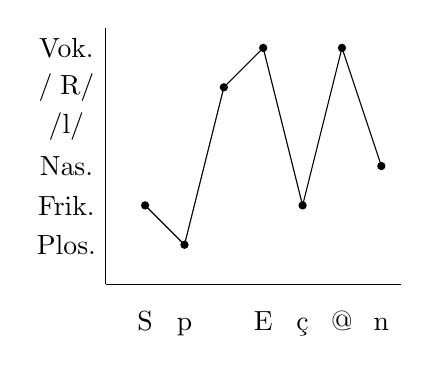
\begin{tikzpicture}[scale=0.5]
\draw[black] (-1,0) -- (6.5,0) ; % x axis
\draw[black] (-1,0) -- (-1,6.5); % y axis
\node at (-2,1) {Plos.};
\node at (-2,2) {Frik.};
\node at (-2,3) {Nas.};
\node at (-2,4) {\textipa{/l/}};
\node at (-2,5) {\textipa{/\;R/}};
\node at (-2,6) {Vok.};
\draw[black] (0,2) -- (1,1) -- (2,5) -- (3,6) -- (4,2) -- (5,6) -- (6,3);
\node at (0,-1) {\strut \textipa{S}};
\node at (1,-1) {\strut \textipa{p}};
\node at (2,-1) {\strut \textipa{\textscr}};
\node at (3,-1) {\strut \textipa{E}};
\node at (4,-1) {\strut \textipa{\c{c}}};
\node at (5,-1) {\strut \textipa{@}};
\node at (6,-1) {\strut \textipa{n}};
\fill (0,2) circle [radius=3pt];
\fill (1,1) circle [radius=3pt];
\fill (2,5) circle [radius=3pt];
\fill (3,6) circle [radius=3pt];
\fill (4,2) circle [radius=3pt];
\fill (5,6) circle [radius=3pt];
\fill (6,3) circle [radius=3pt];
\end{tikzpicture}}}
\end{figure}
\end{minipage}
\pause
\begin{minipage}{.05\textwidth}
\hfill
\end{minipage}
\begin{minipage}{.45\textwidth}
\begin{figure}
\centering
%\visible<4->
{\scalebox{.75}{
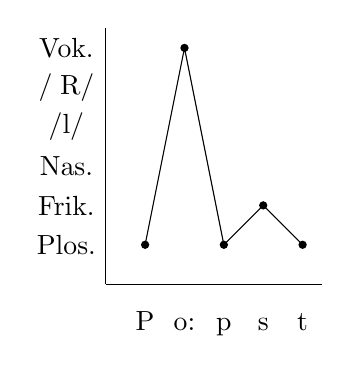
\begin{tikzpicture}[scale=0.5]
\draw[black] (-1,0) -- (4.5,0) ; % x axis
\draw[black] (-1,0) -- (-1,6.5); % y axis
\node at (-2,1) {Plos.};
\node at (-2,2) {Frik.};
\node at (-2,3) {Nas.};
\node at (-2,4) {\textipa{/l/}};
\node at (-2,5) {\textipa{/\;R/}};
\node at (-2,6) {Vok.};
\draw[black] (0,1) -- (1,6) -- (2,1) -- (3,2) -- (4,1);
\node at (0,-1) {\strut \textipa{P}};
\node at (1,-1) {\strut \textipa{o:}};
\node at (2,-1) {\strut \textipa{p}};
\node at (3,-1) {\strut \textipa{s}};
\node at (4,-1) {\strut \textipa{t}};
\fill (0,1) circle [radius=3pt];
\fill (1,6) circle [radius=3pt];
\fill (2,1) circle [radius=3pt];
\fill (3,2) circle [radius=3pt];
\fill (4,1) circle [radius=3pt];
\end{tikzpicture}}}
\end{figure}
\end{minipage}

\end{frame}
%%%%%%%%%%%%%%%%%%%%%%%%%%%%%%%%%

\begin{frame}
\frametitle{Übung -- Lösung}
%
\begin{minipage}{.3\textwidth}
\centering
\scalebox{.75}{\begin{forest} MyP edges, [,phantom
[$\sigma$
[O
[x, tier=word[\textipa{b}]]
[x, tier=word[\textipa{\textscr}]]
]
[R
[N	[x, tier=word[\textipa{a}]]
]
[K
[x[\textipa{n}]]
[x[\textipa{t}]]
]
]  
]
[$\sigma$
[O	[x, tier=word[\textipa{S}]]
]
[R	
[N	
[x[\textipa{U}]]
]
[K	
[x[\textipa{\t{ts}}]]
]
]
]]
\end{forest}}

\end{minipage}
\pause
%
\begin{minipage}{.02\textwidth}
\hfill
\end{minipage}
%
\begin{minipage}{.65\textwidth}
\centering
\scalebox{.75}{
\begin{forest}
MyP edges, [, phantom
[$ \sigma $
[O
[x, tier=word[\textipa{P}]]
]
[R
[N
[x, tier=word[\textipa{a}]]
]
[K
[x[\textipa{p}]]
]
]
]
[$ \sigma $
[O
[x, tier=word[\textipa{S}]]
[x, tier=word[\textipa{t}]]
]
[R
[N
[x[\textipa{a}]]
]
[K
[x[\textipa{n}]]
[x[\textipa{t}]]
[x[\textipa{s}]]
]
]
]
[$ \sigma $
[O
[x, tier=word[\textipa{h}]]
]
[R
[N
[x[\textipa{a}]]
]
[K
[x[\textipa{l}]]
]
]
]
[$ \sigma $
[O
[x, tier=word[t]]
]
[R	
[N
[x[\textipa{\textturna}]]
]
]
]]
\end{forest}}
\end{minipage}
\pause
\begin{minipage}{.3\textwidth}
\begin{figure}
\centering
\scalebox{.75}{
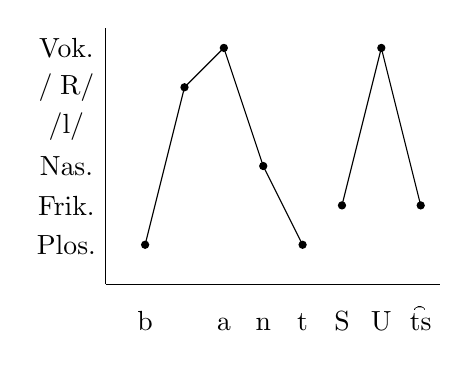
\begin{tikzpicture}[scale=0.5]
\draw[black] (-1,0) -- (7.5,0) ; % x axis
\draw[black] (-1,0) -- (-1,6.5); % y axis
\node at (-2,1) {Plos.};
\node at (-2,2) {Frik.};
\node at (-2,3) {Nas.};
\node at (-2,4) {\textipa{/l/}};
\node at (-2,5) {\textipa{/\;R/}};
\node at (-2,6) {Vok.};
\draw[black] (0,1) -- (1,5) -- (2,6) -- (3,3) -- (4,1);
\draw[black] (5,2) -- (6,6) -- (7,2);
\node at (0,-1) {\strut \textipa{b}};
\node at (1,-1) {\strut \textipa{\textscr}};
\node at (2,-1) {\strut \textipa{a}};
\node at (3,-1) {\strut \textipa{n}};
\node at (4,-1) {\strut \textipa{t}};
\node at (5,-1) {\strut \textipa{S}};
\node at (6,-1) {\strut \textipa{U}};
\node at (7,-1) {\strut \textipa{\t{ts}}};
\fill (0,1) circle [radius=3pt];
\fill (1,5) circle [radius=3pt];
\fill (2,6) circle [radius=3pt];
\fill (3,3) circle [radius=3pt];
\fill (4,1) circle [radius=3pt];
\fill (5,2) circle [radius=3pt];
\fill (6,6) circle [radius=3pt];
\fill (7,2) circle [radius=3pt];
\end{tikzpicture}}
\end{figure}
\end{minipage}
\pause
\begin{minipage}{.05\textwidth}
\hfill
\end{minipage}
\begin{minipage}{.6\textwidth}
\begin{figure}
\centering
\scalebox{.75}{
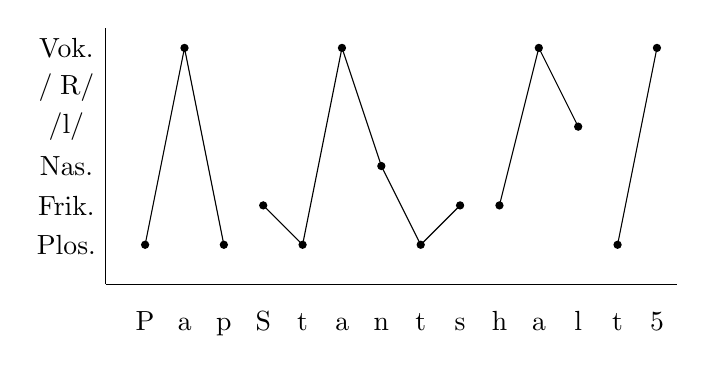
\begin{tikzpicture}[scale=0.5]
\draw[black] (-1,0) -- (13.5,0) ; % x axis
\draw[black] (-1,0) -- (-1,6.5); % y axis
\node at (-2,1) {Plos.};
\node at (-2,2) {Frik.};
\node at (-2,3) {Nas.};
\node at (-2,4) {\textipa{/l/}};
\node at (-2,5) {\textipa{/\;R/}};
\node at (-2,6) {Vok.};
\draw[black] (0,1)--(1,6)--(2,1);
\draw[black](3,2)--(4,1)--(5,6)--(6,3)--(7,1)--(8,2);
\draw[black](9,2)--(10,6)--(11,4);
\draw[black](12,1)--(13,6);
\fill (0,1) circle [radius=3pt];
\fill (1,6) circle [radius=3pt];
\fill (2,1) circle [radius=3pt];
\fill (3,2) circle [radius=3pt];
\fill (4,1) circle [radius=3pt];
\fill (5,6) circle [radius=3pt];
\fill (6,3) circle [radius=3pt];
\fill (7,1) circle [radius=3pt];
\fill (8,2) circle [radius=3pt];
\fill (9,2) circle [radius=3pt];
\fill (10,6) circle [radius=3pt];
\fill (11,4) circle [radius=3pt];
\fill (12,1) circle [radius=3pt];
\fill (13,6) circle [radius=3pt];
\node at (0,-1){\strut \textipa{P}};
\node at (1,-1){\strut \textipa{a}};
\node at (2,-1){\strut \textipa{p}};
\node at (3,-1){\strut \textipa{S}};
\node at (4,-1){\strut \textipa{t}};
\node at (5,-1){\strut \textipa{a}};
\node at (6,-1){\strut \textipa{n}};
\node at (7,-1){\strut \textipa{t}};
\node at (8,-1){\strut \textipa{s}};
\node at (9,-1){\strut \textipa{h}};
\node at (10,-1){\strut \textipa{a}};
\node at (11,-1){\strut \textipa{l}};
\node at (12,-1){\strut \textipa{t}};
\node at (13,-1){\strut \textipa{5}};
\end{tikzpicture}}
\end{figure}
\end{minipage}


\end{frame}

}

%%%%%%%%%%%%%%%%%%%%%%%%%%%%%%%%%%


%%%%%%%%%%%%%%%%%%%%%%%%%%%%%%%%%%
\subsection{Silbifizierung}

%% MyP: Contents
\iftoggle{sectoc}{
	\frame{
		%\begin{multicols}{2}
		\frametitle{~}
		\tableofcontents[currentsubsection, subsubsectionstyle=hide]
		%\end{multicols}
	}
}

%% StM: Contents
\iftoggle{gliederung}{
	
	\outline{
		\begin{itemize}
			
			\item Silbenmodelle
			%% CV-Modell
			%% Konstituentenmodell
			\item Silbengelenk
			\item \blaubf{Silbifizierung}
			\item Exkurs: Akzent
			\item Hausaufgabe
			
		\end{itemize}
	}
}
%%%%%%%%%%%%%%%%%%%%%%%%%%%%%%%%%%

\begin{frame}
\frametitle{Silbifizierung}

\begin{block}{Silbifizierung (auch Syllabierung)}
	Wörter in Silben einteilen
\end{block}

\begin{itemize}
	\item Wie würden Sie folgende Lautsequenzen silbifizieren?
	
	\ea ata, odo, eke
	\z
	
	\pause
	
	\item Ein einziger intervokalischer Konsonant wird immer als Silbenanlaut silbifiziert (universelles Prinzip: \textbf{Onset-Maximierung}).


\end{itemize}

\begin{block}{Onset-Maximierung}
Bilde zuerst den größtmöglichen Silbenanlaut;\\
dann bilde den Silbenauslaut \citep[218]{Hall00a}.
\end{block}

\end{frame}


%%%%%%%%%%%%%%%%%%%%%%%%%%%%%%%%%%
\begin{frame}
\frametitle{Onset-Maximierung}

\begin{block}{Onset-Maximierung}
Bilde zuerst den größtmöglichen Silbenanlaut;\\
dann bilde den Silbenauslaut \citep[218]{Hall00a}.
\end{block}


\begin{itemize}
\item Onset-Maximierung herleitbar aus:
\begin{enumerate}
\item Silbenanlautgesetz (CV häufiger als V), und
\item Silbenauslautgesetz (CVC$^{n} >$ CVC$^{n+1}$, wobei $n \geq 0$)
\end{enumerate}

\pause
\item Silbifizierung nicht über Morphemgrenzen hinweg! (grob: Morphem = kleinste bedeutungstragende Einheit)
\item Ausnahme: Suffixe mit vokalischem Onset:

\ea
kind\#isch: \textipa{[kIn.dIS]}

\ex
kind\#lich: \textipa{[kInt.lI\c{c}]}
\z

\item \# := Morphemgrenze

% Wenn man Morphmgrenzenbedingung weglassen würde, ergäbe sich Bra. ndschutz

% rek.nen vs. re.gnen

\end{itemize}

\end{frame}


%%%%%%%%%%%%%%%%%%%%%%%%%%%%%%%%%%
%\subsection{Übung}
%
%%% MyP: Contents
%\iftoggle{sectoc}{
%	\frame{
%		%\begin{multicols}{2}
%		\frametitle{~}
%		\tableofcontents[currentsubsection, subsubsectionstyle=hide]
%		%\end{multicols}
%	}
%}
%%%%%%%%%%%%%%%%%%%%%%%%%%%%%%%%%%
\begin{frame}
\frametitle{Übung}

\begin{itemize}
	\item Was bedeutet die Annahme des Sonoritätsprinzips und der Onset-Maximierung für die folgenden Beispielwörter?
	
	\eal\label{ex:fabrik}
	\ex Fabrik
	\ex Imker
	\ex neblig
	\ex Falter
	\ex regnen
	\zl
\end{itemize}

\end{frame}


%%%%%%%%%%%%%%%%%%%%%%%%%%%%%%%%
\iftoggle{ue-loesung}{
	%%%%%%%%%%%%%%%%%%%%%%%%%%%%%%%%%%
%% UE 2 - 03c Phonologie
%%%%%%%%%%%%%%%%%%%%%%%%%%%%%%%%%%


\begin{frame}
\frametitle{Übung -- Lösung}

\begin{itemize}
	\item Was bedeutet die Annahme des Sonoritätsprinzips und der Onset-Maximierung für die folgenden Beispielwörter?
	
	\begin{exe}
	\exr{ex:fabrik}
	\settowidth\jamwidth{XXXXXXXXXXXXXXXXXXXXXXXXXXXXXXXXXXXX}
	\begin{xlist}
		\ex Fabrik\loesung{1}{\textipa{[fa.b\textscr ik]} (auch: \textipa{[fa.b\;Ri:k]} oder \textipa{[fa.b\;RIk]})}
		\ex Imker\loesung{2}{\textipa{[PIm.k5]}}
		\ex neblig\loesung{3}{\textipa{[ne:.blI\c{c}]}}
		\ex Falter\loesung{4}{\textipa{[fal.t5]}}
		\ex regnen\loesung{5}{\textipa{[\textscr e:.gn@n]}}
		
	\loesung{6}{Onset: Obstruent vor Sonorant}
	\loesung{6}{Koda: Sonorant vor Obstruent}
	
	\end{xlist}
\end{exe}
	
\visible<7->{
\alertgreen{
	Onset-Maximierung ist nicht strikt. Alternativ ginge auch \textipa{[ne:p.lI\c{c}]}, \textipa{[\textscr e:k.n@n]}.
}
}
	
\end{itemize}

\end{frame}	

}

%%%%%%%%%%%%%%%%%%%%%%%%%%%%%%%
\begin{frame}{Übung}

\begin{itemize}
	\item Welche Prinzipien bzw. Regularitäten werden verletzt bei:


	\eal\label{ex:ebbe}
	\ex \textipa{[PE.b@]}
	\ex \textipa{[PEb.@]}
	\ex \textipa{[PEp.@]}
	\ex \textipa{[PEp.b@]}
	\zl
	
\end{itemize}

\end{frame}


%%%%%%%%%%%%%%%%%%%%%%%%%%%%%%%%
\iftoggle{ue-loesung}{
	%%%%%%%%%%%%%%%%%%%%%%%%%%%%%%%%%%
%% UE 3 - 03c Phonologie
%%%%%%%%%%%%%%%%%%%%%%%%%%%%%%%%%%

\begin{frame}
\frametitle{Übung -- Lösung}
	\begin{itemize}

	\item Welche Prinzipien bzw. Regularitäten werden verletzt bei:

\begin{exe}
	\exr{ex:ebbe}
	\settowidth\jamwidth{XXXXXXXXXXXXXXXXXXXXXXXXXXXXXXXXXXXX}
	\begin{xlist}
		\ex \textipa{[PE.b@]}\loesung{1}{\ras Kurzvokalregel, Lösung \zb Silbengelenk \textipa{[PE\.b@]}}
		\ex \textipa{[PEb.@]}\loesung{2}{\ras Auslautverhärtung}
		\ex \textipa{[PEp.@]}\loesung{3}{\ras Onset-Maximierung}
		\ex \textipa{[PEp.b@]}\loesung{4}{\ras keine Regelverletzung}
	\end{xlist}
\end{exe}

	\end{itemize}

\end{frame}

}

%%%%%%%%%%%%%%%%%%%%%%%%%%%%%%%
\begin{frame}
\frametitle{Übung}

\begin{itemize}
	\item Silbifizieren Sie folgende Segmentsequenzen \textbf{in zwei Schritten}:
	\begin{itemize}
		\item Onset-Maximierungsprinzip
		\item Sonoritätsprinzip
	\end{itemize}
	
	\item Stellen Sie fest, ob alle Silben wohlgeformt sind.\\
	Falls nicht, benennen Sie die Verletzungen.
	
	\ea\label{ex:otling}
	\textipa{[o:tlIN5mSplag\textscr e:hOn]}
	\z
	
	% Otlingamsplagrehon
	
	\ea\label{ex:blumen}
	Blumentopferde
	\z
	
\end{itemize}

% blu.men.to.pfer.de

%\ea
%Urinstinkt
%\z	

\end{frame}


%%%%%%%%%%%%%%%%%%%%%%%%%%%%%%%%%%
\iftoggle{ue-loesung}{
	%%%%%%%%%%%%%%%%%%%%%%%%%%%%%%%%%%
%% UE 4 - 03c Phonologie
%%%%%%%%%%%%%%%%%%%%%%%%%%%%%%%%%%

\begin{frame}
\frametitle{Übung -- Lösung}

\begin{itemize}
\item Silbifizieren Sie folgende Segmentsequenzen \textbf{in zwei Schritten}:
\begin{itemize}
	\item Onsetmaximierungsprinzip
	\item Sonoritätsprinzip
\end{itemize}

\item Stellen Sie fest, ob alle Silben wohlgeformt sind.\\
Falls nicht, benennen Sie die Verletzungen.

\begin{exe}
	\exr{ex:otling}
	\textipa{[o:tlIN5mSplag\textscr e:hOn]}\\
	\alertgreen{zuerst Onset"=Maximierung: \textipa{o: . tlI . \ng {\textturna} . mSpla . g\textscr e: . hOn}\\
	dann Anwendung des Sonoritätsprinzips: \textipa{o: . tlI\. \ng \textturna mS . pla . g\textscr e: . hOn}}
\end{exe}

% Otlingamsplagrehon

\begin{exe}
	\exr{ex:blumen}
	Blumentopferde\\ \pause
	\alertgreen{zuerst Onset-Maximierung: \textipa{blu: . m@ . ntO . pfE . {\textscr}d@}\\
	dann Awendung des Sonoritätsprinzips: \textipa{blu: . m@n . tO . pfE{\textscr} . d@}}
\end{exe}

\end{itemize}

% blu.men.to.pfer.de

%\ea
%Urinstinkt
%\z	

\end{frame}


% ' Stahl , tische     Hauptbetonung auf Stahl, Nebenbetonung auf Tische


}

%%%%%%%%%%%%%%%%%%%%%%%%%%%%%%%%%%


%%%%%%%%%%%%%%%%%%%%%%%%%%%%%%%%%%
\subsection{Exkurs: Akzent}
%%%%%%%%%%%%%%%%%%%%%%%%%%%%%%%%%%

%% MyP: Contents
\iftoggle{sectoc}{
	\frame{
		%\begin{multicols}{2}
		\frametitle{~}
		\tableofcontents[currentsubsection, subsubsectionstyle=hide]
		%\end{multicols}
	}
}

%% StM: Contents
\iftoggle{gliederung}{
	
	\outline{
		\begin{itemize}
			
			\item Silbenmodelle
			%% CV-Modell
			%% Konstituentenmodell
			\item Silbengelenk
			\item Silbifizierung
			\item \blaubf{Exkurs: Akzent}
			\item Hausaufgabe
			
		\end{itemize}
	}
}
%%%%%%%%%%%%%%%%%%%%%%%%%%%%%%%%%%

\begin{frame}
\frametitle{Exkurs: Akzent}

\begin{itemize}
\item Silben können \textbf{betont} oder \textbf{unbetont} sein, d.\,h. sie können einen Akzent tragen oder nicht.
\item[]

\begin{block}{Akzent}
\textbf{Auditiver Eindruck der Prominenz eines Vokals} gegenüber einem anderen durch (relational, nicht absolut!):
\begin{itemize}
\item Lautstärke
\item Dauer
\item Höhere Tonlage
\item Ausgeprägtere Artikulationsbewegungen
\end{itemize}
\end{block}	 

\item[]
\item Man unterscheidet zwischen \textbf{Wort-} und \textbf{Satzakzent} (engl. \emph{stress} und \emph{accent}).

\end{itemize}

\end{frame}



%%%%%%%%%%%%%%%%%%%%%%%%%%%%%%%%%%%
%%%%%%%%%%%%%%%%%%%%%%%%%%%%%%%%%%
%\subsubsection{Exkurs: Wortakzent}
%\frame{
%\begin{multicols}{2}
%\frametitle{~}
%	\tableofcontents[currentsection]
%\end{multicols}
%}
%%%%%%%%%%%%%%%%%%%%%%%%%%%%%%%%%%

\begin{frame}
\frametitle{Exkurs: Wortakzent}

\begin{itemize}
\item Was scheint die häufigste Betonung im Deutschen zu sein?

\ea
Mutter, Männer, Autos, Hühner, Lehrer, Kinder, alle, \ldots
\z

\pause
\textbf{betont-unbetont (Trochäus)}

\item Ausnahmen (die je nach Theorie verschieden erklärt werden):

\end{itemize}

\begin{minipage}{.4\textwidth}

\eal 
\ex \textipa{['f\textscr aU]}
\ex \textipa{[mu.'zi:k]}
\ex \textipa{['le:.b@n.d@]}
\ex \textipa{[pa.pa.'g\t{aɪ}]}
\ex \textipa{[f\t{ɛɐ}.'Pa\textscr .b\t{aɪ}.t@n]}
\zl

\end{minipage}
\begin{minipage}{.5\textwidth}

%	\iftoggle{loesung}{
\begin{itemize}
\item[] \alertred{\ras nur eine Silbe }
\item[] \alertred{\ras Fremdwort}
\item[] \alertred{\ras flektierte Elemente \ab{-de}}
\item[] \alertred{\ras Fremdwort}
\item[] \alertred{\ras Derivation \ab{ver-}}
\end{itemize}
%}

\end{minipage}

\end{frame}



%%%%%%%%%%%%%%%%%%%%%%%%%%%%%%%%%%%
%%%%%%%%%%%%%%%%%%%%%%%%%%%%%%%%%%
%\subsubsection{Exkurs: Satzakzent}
%\frame{
%\begin{multicols}{2}
%\frametitle{~}
%	\tableofcontents[currentsection]
%\end{multicols}
%}
%%%%%%%%%%%%%%%%%%%%%%%%%%%%%%%%%%

\begin{frame}
\frametitle{Exkurs: Satzakzent}

\begin{itemize}
\item In einem Satz können betonte Silben \textbf{noch weiter hervorgehoben} werden (dabei meist durch die Tonhöhe):

\eal 
\ex Géstern hat BÁyern gewónnen.
\ex GÉStern hat Báyern gewónnen.
\ex Géstern hat Báyern geWÓNnen.
\zl
\item Die prominenteste Silbe im Satz wird meist mit \textbf{Großbuchstaben} dargestellt, sie trägt den Satzakzent.

\item Durch diese Akzentuierung wird das gesamte Wort
hervorgehoben.\\
\ras \textbf{Fokus des Satzes} (\gqq{Informationsstruktur})

\end{itemize}

\end{frame}



%%%%%%%%%%%%%%%%%%%%%%%%%%%%%%%%%%%
%%%%%%%%%%%%%%%%%%%%%%%%%%%%%%%%%%
%\subsubsection{Exkurs: Intonation}
%\frame{
%\begin{multicols}{2}
%\frametitle{~}
%	\tableofcontents[currentsection]
%\end{multicols}
%}
%%%%%%%%%%%%%%%%%%%%%%%%%%%%%%%%%%

\begin{frame}
\frametitle{Exkurs: Intonation}

\begin{block}{Intonation}
Tonhöhenverlauf (\gqq{Melodie}) einer Äußerung
\end{block}

\begin{itemize}
\item \textbf{Satztypen} können mittels Intonation unterschieden werden.

\item Sprechen Sie die folgenden Äußerungen mit fallender und steigender Intonation.
\eal 
\ex Heute gewinnen die Bayern.
\ex Schon Schluss.
\zl
\pause
\textbf{Aussage-} \vs \textbf{Interrogativsatz}	

\end{itemize}

\end{frame}



%%%%%%%%%%%%%%%%%%%%%%%%%%%%%%%%%%

\begin{frame}
\frametitle{Disambiguierung}

Ambige ($\approx$ mehrdeutige) Sätze können mittels Intonation \gs{durch die sog. Hutkontur} \textbf{disambiguiert} werden: 

\begin{exe}
\ex  \label{exe:nicht}Alle Studenten haben die Klausur nicht bestanden.

	\begin{xlist}
	\ex Es ist nicht der Fall, dass alle Studenten die Klausur bestanden haben. \hfill $\lsem \neg \forall \rsem$
	\ex Für alle Studenten gilt, dass sie die Klausur nicht bestanden haben. \hfill $\lsem \forall \neg \rsem$
	\end{xlist}

\pause 

\ex /ALle Studenten haben die Klausur  NICHT\textbackslash\ bestanden.
\exr{exe:nicht}
	\begin{xlist}
	\ex Es ist nicht der Fall, dass alle Studenten die Klausur bestanden haben. \hfill $\lsem \neg \forall \rsem$
	\end{xlist}
\end{exe}


\end{frame}


%%%%%%%%%%%%%%%%%%%%%%%%%%%%%%%%%%
\subsection{Hausaufgabe}
%%%%%%%%%%%%%%%%%%%%%%%%%%%%%%%%%%

%%% MyP: Contents
%\iftoggle{sectoc}{
%	\frame{
%		%\begin{multicols}{2}
%		\frametitle{~}
%		\tableofcontents[currentsubsection, subsubsectionstyle=hide]
%		%\end{multicols}
%	}
%}

%%% StM: Contents
%\iftoggle{gliederung}{
%	
%	\outline{
%		\begin{itemize}
%			
%			\item Silbenmodelle
%			%% CV-Modell
%			%% Konstituentenmodell
%			\item Silbengelenk
%			\item Silbifizierung
%			\item Exkurs: Akzent
%			\item \blaubf{Hausaufgabe}
%			
%		\end{itemize}
%	}
%}


%%%%%%%%%%%%%%%%%%%%%%%%%%%%%%%%%%
\begin{frame}%[allowframebreaks]
\frametitle{Hausaufgabe}
\begin{itemize}

\item[1.] Geben Sie eine \textbf{phonetische Transkription} der folgenden Wörter nach der \gqq{Standardaussprache} an, zeichnen Sie dabei die \textbf{Silbenstruktur} nach dem \textbf{Konstituentenmodell} und mit der \textbf{Skelettschicht} und geben Sie die \textbf{Sonoritätsprofile} an.

\eal\label{ex:03cHA1}
\ex Stimmenfang \label{ex:03cHA1a}
\ex Mittagessen\label{ex:03cHA1b}
\ex Bierdeckel\label{ex:03cHA1c}
\zl
\end{itemize}

\begin{block}{Sonoritätshierarchie (Zur Erinnerung)}
Vokal $>$ \textipa{/\textscr /} $>$ \textipa{/l/} $>$ Nasal $>$ Frikativ $>$ Plosiv \\
$x > y$ := $x$ ist sonorer als $y$
\end{block}

\end{frame}

%%%%%%%%%%%%%%%%%%%%%%%%%%%%%%%%%%%%%%%%%%%%%%%%%%%%%

\begin{frame}
\begin{itemize}
\item[2.] Silbifizieren Sie folgende Segmentsequenzen \textbf{in zwei Schritten}:
\begin{itemize}
\item Onset-Maximierungsprinzip
\item Sonoritätsprinzip
\end{itemize}

Stellen Sie fest, ob alle Silben wohlgeformt sind. Falls nicht, benennen Sie die Verletzungen.
\ea\label{ex:03cHA2}
Urinstinkt
\z	
\item[3.] Geben Sie die standarddeutsche \textbf{phonetische Transkription} des Wortes \ab{Stahltische} inklusive der \textbf{Silbenstruktur} (mit X-Skelettschicht) an.\\Ermitteln Sie die \textbf{Kriterien}, die bei der Silbifizierung wirken.

\item[4.] Geben Sie die Gründe an, warum die folgenden Wörter aus phonetisch"=phonologischen Gründen im Deutschen nicht möglich sind:

\eal\label{ex:03cHA3}
\ex[*]{\textipa{['Napl.O:t]}}
\ex[*]{\textipa{[a\;R.'tUng]}}
\zl

\end{itemize}

\end{frame}

%%%%%%%%%%%%%%%%%%%%%%%%%%%%%%%%%%%
\iftoggle{ha-loesung}{
	%%%%%%%%%%%%%%%%%%%%%%%%%%%%%%%%%%
%% HA 1 - 03c Phonologie
%%%%%%%%%%%%%%%%%%%%%%%%%%%%%%%%%%

\begin{frame}%[allowframebreaks]
\frametitle{Hausaufgabe -- Lösung}
\begin{itemize}

\item[1.] Geben Sie eine \textbf{phonetische Transkription} der folgenden Wörter nach der \gqq{Standardaussprache} an, zeichnen Sie dabei die \textbf{Silbestruktur} nach dem \textbf{Konstituentenmodell} und mit der \textbf{Skelettschicht} und geben Sie die \textbf{Sonoritätsprofile} an.

\begin{exe}
\exi{(\ref{ex:03cHA1})}
\begin{xlist}
\ex Stimmenfang
\ex Mittagessen
\ex Bierdeckel
\end{xlist}
\end{exe}

\begin{block}{Sonoritätshierarchie (zur Erinnerung)}
Vokal $>$ \textipa{/\textscr /} $>$ \textipa{/l/} $>$ Nasal $>$ Frikativ $>$ Plosiv \\
$x > y :=$ $x$ ist sonorer als $y$
\end{block}

\end{itemize}
\end{frame}
%%%%%%%%%%%%%%%%%%%%%%%%%%%%%%%%%%

\begin{frame}{Hausaufgabe -- Lösung}

Zu (\ref{ex:03cHA1a}) Stimmenfang:

\begin{columns}	
	
\column[b]{.5\textwidth}

\begin{figure}
%	\footnotesize
	\centering
	\begin{forest} MyP edges, [, phantom
		[$\sigma$
		[O [x, tier=word [\textipa{S}]] [x, tier=word [\textipa{t}]]]
		[R [N [x, tier=word [\textipa{I}]]] [K [x, name=x [\textipa{m}]]]]
		]
		[$\sigma$
		[O, name=onset]
		[R [N [x [\textipa{@}]]] [K [x [\textipa{n}]]]]
		]
		[$\sigma$
		[O [x, tier=word [\textipa{f}]]]
		[R [N [x [\textipa{a}]]] [K [x [\textipa{N}]]]]
		]
		]				
		{
		\draw[black] (x.north)--(onset.south);
		}
	\end{forest}
\end{figure}

\pause

\column[b]{.5\textwidth}

\begin{figure}
%	\footnotesize
	\centering	
	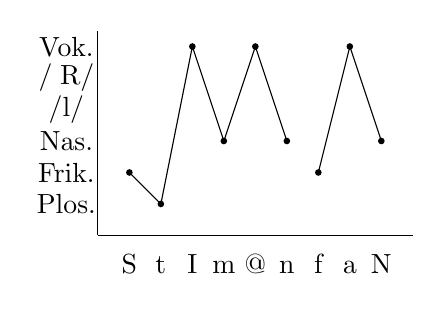
\begin{tikzpicture}[scale=0.4]
		\draw[black] (-1,0) -- (9,0) ; % x axis
		\draw[black] (-1,0) -- (-1,6.5); % y axis
		\node at (-2,1) {Plos.};
		\node at (-2,2) {Frik.};
		\node at (-2,3) {Nas.};
		\node at (-2,4) {\textipa{/l/}};
		\node at (-2,5) {\textipa{/\;R/}};
		\node at (-2,6) {Vok.};
		\draw[black] (0,2) -- (1,1) -- (2,6) -- (3,3) -- (4,6) -- (5,3);
		\draw[black] (6,2) -- (7,6) -- (8,3);
		\node at (0,-1) {\strut \textipa{S}};
		\node at (1,-1) {\strut \textipa{t}};
		\node at (2,-1) {\strut \textipa{I}};
		\node at (3,-1) {\strut \textipa{m}};
		\node at (4,-1) {\strut \textipa{@}};
		\node at (5,-1) {\strut \textipa{n}};
		\node at (6,-1) {\strut \textipa{f}};
		\node at (7,-1) {\strut \textipa{a}};
		\node at (8,-1) {\strut \textipa{N}};
		\fill (0,2) circle [radius=3pt];
		\fill (1,1) circle [radius=3pt];
		\fill (2,6) circle [radius=3pt];
		\fill (3,3) circle [radius=3pt];
		\fill (4,6) circle [radius=3pt];
		\fill (5,3) circle [radius=3pt];
		\fill (6,2) circle [radius=3pt];
		\fill (7,6) circle [radius=3pt];
		\fill (8,3) circle [radius=3pt];
	\end{tikzpicture}
\end{figure}

\end{columns}

\end{frame}


%%%%%%%%%%%%%%%%%%%%%%%%%%%%%%%%%%%%%%%%%%%%%%%
\begin{frame}{Hausaufgabe -- Lösung}


Zu (\ref{ex:03cHA1b}) Mittagessen:

\begin{columns}
	\column[b]{.5\textwidth}
	
\begin{figure}
\footnotesize
\centering
\begin{forest} MyP edges, [, phantom
	[$\sigma$
	[O [x, tier=word [\textipa{m}]]] 
	[R [N [x, tier=word [\textipa{I}]]] [K [x, name=x1 [\textipa{t}]]]]
	]
	[$\sigma$
	[O, name=onset1]
	[R [N [x [\textipa{a:}, name=a]]
	[x, name=ax]] [K [x [\textipa{k}]]]]
	]
	[$\sigma$
	[O [x, tier=word [\textipa{P}]]]
	[R [N [x [\textipa{E}]]] [K [x, name=x2 [\textipa{s}]]]]
	]
	[$\sigma$
	[O, name=onset2]
	[R [N [x [\textipa{@}]]] [K [x [\textipa{n}]]]]
	]
	]
	{
		\draw[black] (x1.north)--(onset1.south);
		\draw[black] (x2.north)--(onset2.south);
		\draw[black] (a.north)--(ax.south);
	}
\end{forest}

\end{figure}

\pause

\column[b]{.5\textwidth}

\begin{figure}
\footnotesize
\centering
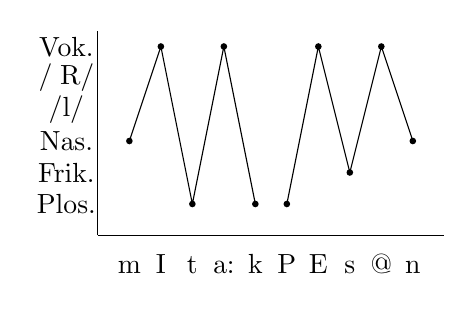
\begin{tikzpicture}[scale=0.4]
\draw[black] (-1,0) -- (10,0) ; % x axis
\draw[black] (-1,0) -- (-1,6.5); % y axis
\node at (-2,1) {Plos.};
\node at (-2,2) {Frik.};
\node at (-2,3) {Nas.};
\node at (-2,4) {\textipa{/l/}};
\node at (-2,5) {\textipa{/\;R/}};
\node at (-2,6) {Vok.};
\draw[black] (0,3) -- (1,6) -- (2,1) -- (3,6) -- (4,1);
\draw[black] (5,1) -- (6,6) -- (7,2) -- (8,6) -- (9,3);
\node at (0,-1) {\strut \textipa{m}};
\node at (1,-1) {\strut \textipa{I}};
\node at (2,-1) {\strut \textipa{t}};
\node at (3,-1) {\strut \textipa{a:}};
\node at (4,-1) {\strut \textipa{k}};
\node at (5,-1) {\strut \textipa{P}};
\node at (6,-1) {\strut \textipa{E}};
\node at (7,-1) {\strut \textipa{s}};
\node at (8,-1) {\strut \textipa{@}};
\node at (9,-1) {\strut \textipa{n}};
\fill (0,3) circle [radius=3pt];
\fill (1,6) circle [radius=3pt];
\fill (2,1) circle [radius=3pt];
\fill (3,6) circle [radius=3pt];
\fill (4,1) circle [radius=3pt];
\fill (5,1) circle [radius=3pt];
\fill (6,6) circle [radius=3pt];
\fill (7,2) circle [radius=3pt];
\fill (8,6) circle [radius=3pt];
\fill (9,3) circle [radius=3pt];
\end{tikzpicture}
\end{figure}

\end{columns}

\end{frame}


%%%%%%%%%%%%%%%%%%%%%%%%%%%%%%%%%%%%%%%%%%%%
\begin{frame}{Hausaufgabe -- Lösung}

Zu (\ref{ex:03cHA1b}) Mittagessen (alternative Lösung):

\begin{columns}
	\column[b]{.5\textwidth}
	
	
\begin{figure}
\footnotesize
\centering

		\begin{forest} MyP edges, [, phantom
		[$\sigma$
		[O [x, tier=word [\textipa{m}]]] 
		[R [N [x, tier=word [\textipa{I}]]] [K [x, name=x1 [\textipa{t}]]]]
		]
		[$\sigma$
		[O, name=onset1]
		[R [N [x [\textipa{a:}, name=a]]
		[x, name=ax]] [K [x [\textipa{k}]]]]
		]
		[$\sigma$
		[O [x, tier=word [\textipa{P}]]]
		[R [N [x [\textipa{E}]]] [K [x, name=x2 [\textipa{s}]]]]
		]
		[$\sigma$
		[O, name=onset2]
		[R [N [x [\textipa{\textsyllabic{n}}]]] [K]
		]
		]]
		{
			\draw[black] (x1.north)--(onset1.south);
			\draw[black] (x2.north)--(onset2.south);
			\draw[black] (a.north)--(ax.south);
		}
	\end{forest}
\end{figure}

\pause
\column[b]{.5\textwidth}

\begin{figure}
\footnotesize
\centering
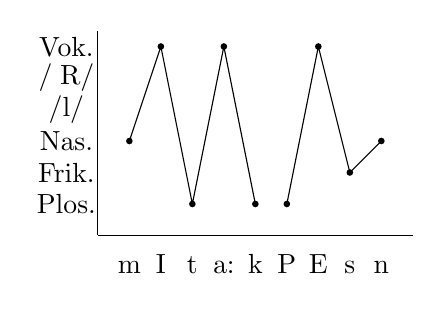
\begin{tikzpicture}[scale=0.4]
\draw[black] (-1,0) -- (9,0) ; % x axis
\draw[black] (-1,0) -- (-1,6.5); % y axis
\node at (-2,1) {Plos.};
\node at (-2,2) {Frik.};
\node at (-2,3) {Nas.};
\node at (-2,4) {\textipa{/l/}};
\node at (-2,5) {\textipa{/\;R/}};
\node at (-2,6) {Vok.};
\draw[black] (0,3) -- (1,6) -- (2,1) -- (3,6) -- (4,1);
\draw[black] (5,1) -- (6,6) -- (7,2) -- (8,3);
\node at (0,-1) {\strut \textipa{m}};
\node at (1,-1) {\strut \textipa{I}};
\node at (2,-1) {\strut \textipa{t}};
\node at (3,-1) {\strut \textipa{a:}};
\node at (4,-1) {\strut \textipa{k}};
\node at (5,-1) {\strut \textipa{P}};
\node at (6,-1) {\strut \textipa{E}};
\node at (7,-1) {\strut \textipa{s}};
\node at (8,-1) {\strut \textipa{\textsyllabic{n}}};
\fill (0,3) circle [radius=3pt];
\fill (1,6) circle [radius=3pt];
\fill (2,1) circle [radius=3pt];
\fill (3,6) circle [radius=3pt];
\fill (4,1) circle [radius=3pt];
\fill (5,1) circle [radius=3pt];
\fill (6,6) circle [radius=3pt];
\fill (7,2) circle [radius=3pt];
\fill (8,3) circle [radius=3pt];
\end{tikzpicture}
\end{figure}

\end{columns}

\end{frame}


%%%%%%%%%%%%%%%%%%%%%%%%%%%%%%%%%%%%%%%%%%%%%%%
\begin{frame}{Hausaufgabe -- Lösung}

Zu (\ref{ex:03cHA1c}) Bierdeckel:

\begin{columns}
	\column[b]{.5\textwidth}
	
\begin{figure}
\centering
	\begin{forest} MyP edges, [, phantom
		[$\sigma$
		[O [x,tier=word [\textipa{b}]]]
		[R [N [x, tier=word [\textipa{i:}, name=i]] [x,name=x1][x [\textipa{5}]]] [K]
		]
		]
		[$\sigma$
		[O [x, tier=word [\textipa{d}]]]
		[R [N [x [\textipa{E}]]] [K [x, name=x [\textipa{k}]]]]
		]
		[$\sigma$
		[O, name=onset]
		[R [N [x, tier=word [\textipa{@}]]] [K [x [\textipa{l}]]]]
		]
		]
		{
		\draw[black] (x1.south)--(i.north);
		\draw[black] (x.north)--(onset.south);
		}
	\end{forest}
\end{figure}

\pause

\column[b]{.5\textwidth}

\begin{figure}
\centering
	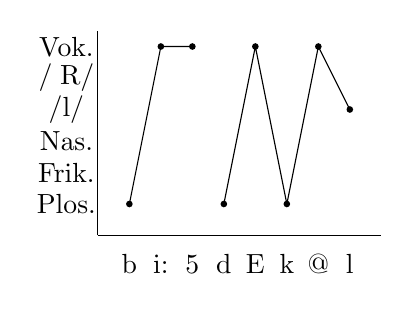
\begin{tikzpicture}[scale=0.4]
		\draw[black] (-1,0) -- (8,0) ; % x axis
		\draw[black] (-1,0) -- (-1,6.5); % y axis
		\node at (-2,1) {Plos.};
		\node at (-2,2) {Frik.};
		\node at (-2,3) {Nas.};
		\node at (-2,4) {\textipa{/l/}};
		\node at (-2,5) {\textipa{/\;R/}};
		\node at (-2,6) {Vok.};
		\draw[black] (0,1) -- (1,6) -- (2,6);
		\draw[black] (3,1) -- (4,6) -- (5,1) -- (6,6) -- (7,4);
		\node at (0,-1) {\strut \textipa{b}};
		\node at (1,-1) {\strut \textipa{i:}};
		\node at (2,-1) {\strut \textipa{5}};
		\node at (3,-1) {\strut \textipa{d}};
		\node at (4,-1) {\strut \textipa{E}};
		\node at (5,-1) {\strut \textipa{k}};
		\node at (6,-1) {\strut \textipa{@}};
		\node at (7,-1) {\strut \textipa{l}};
		\fill (0,1) circle [radius=3pt];
		\fill (1,6) circle [radius=3pt];
		\fill (2,6) circle [radius=3pt];
		\fill (3,1) circle [radius=3pt];
		\fill (4,6) circle [radius=3pt];
		\fill (5,1) circle [radius=3pt];
		\fill (6,6) circle [radius=3pt];
		\fill (7,4) circle [radius=3pt];
	\end{tikzpicture}
\end{figure}

\end{columns}

\end{frame}


%%%%%%%%%%%%%%%%%%%%%%%%%%%%%%%%%%%%%%%%%%%%%%%%%%%
\begin{frame}{Hausaufgabe -- Lösung}

Zu (\ref{ex:03cHA1c}) Bierdeckel (alternative Lösung):

\begin{columns}
	\column[b]{.5\textwidth}
	
	\begin{figure}
		\centering
		\begin{forest} MyP edges, [, phantom
			[$\sigma$
			[O [x,tier=word [\textipa{b}]]]
			[R [N [x, tier=word [\textipa{i:}, name=i]] [x,name=x1][x [\textipa{5}]]] [K]
			]
			]
			[$\sigma$
			[O [x, tier=word [\textipa{d}]]]
			[R [N [x [\textipa{E}]]] [K [x, name=x [\textipa{k}]]]]
			]
			[$\sigma$
			[O, name=onset]
			[R [N [x, tier=word [\textipa{\textsyllabic{l}}]]] [K]
			]
			]
			]
			{
				\draw[black] (x1.south)--(i.north);
				\draw[black] (x.north)--(onset.south);
			}
		\end{forest}
	\end{figure}
	
	\pause
	
	\column[b]{.5\textwidth}
	
	\begin{figure}
		\centering
		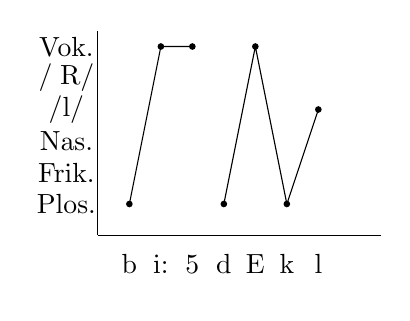
\begin{tikzpicture}[scale=0.4]
		\draw[black] (-1,0) -- (8,0) ; % x axis
		\draw[black] (-1,0) -- (-1,6.5); % y axis
		\node at (-2,1) {Plos.};
		\node at (-2,2) {Frik.};
		\node at (-2,3) {Nas.};
		\node at (-2,4) {\textipa{/l/}};
		\node at (-2,5) {\textipa{/\;R/}};
		\node at (-2,6) {Vok.};
		\draw[black] (0,1) -- (1,6) -- (2,6);
		\draw[black] (3,1) -- (4,6) -- (5,1) -- (6,4);
		\node at (0,-1) {\strut \textipa{b}};
		\node at (1,-1) {\strut \textipa{i:}};
		\node at (2,-1) {\strut \textipa{5}};
		\node at (3,-1) {\strut \textipa{d}};
		\node at (4,-1) {\strut \textipa{E}};
		\node at (5,-1) {\strut \textipa{k}};
		\node at (6,-1) {\strut \textipa{\textsyllabic{l}}};
		\fill (0,1) circle [radius=3pt];
		\fill (1,6) circle [radius=3pt];
		\fill (2,6) circle [radius=3pt];
		\fill (3,1) circle [radius=3pt];
		\fill (4,6) circle [radius=3pt];
		\fill (5,1) circle [radius=3pt];
		\fill (6,4) circle [radius=3pt];
		\end{tikzpicture}
	\end{figure}
	
\end{columns}

\end{frame}


%%%%%%%%%%%%%%%%%%%%%%%%%%%%%%%%%%%%%%%%%%%%%%%%%%
\begin{frame}{Hausaufgabe -- Lösung}
\begin{itemize}
\item[2.] Silbifizieren Sie folgende Segmentsequenzen \textbf{in zwei Schritten}:
\begin{itemize}
\item Onsetmaximierungsprinzip
\item Sonoritätsprinzip
\end{itemize}

Stellen Sie fest, ob alle Silben wohlgeformt sind.\\
Falls nicht, benennen Sie die Verletzungen.

\begin{exe}
\exr{ex:03cHA2} Urinstinkt
\pause
\begin{xlist}
	\settowidth\jamwidth{XXXXXXXXXXXXXXXXXXXXXXXXXXXXXXX}
	\ex \alertgreen{\textipa{[Pu.\;RI.nstINkt]} \jambox{Onsetmaximierung, keine r-Vokalisierung} } \pause
	
	\ex  \alertgreen{\textipa{[Pu.\;RIns.tINkt]} \jambox{Sonoritätsprinzip} } \pause 

	\ex  \alertgreen{\textipa{[Pu5.PIns.tINkt]} \jambox{Silbifizierung der phonologischen Wörter} } \pause
	 
	\exi{} \alertgreen{ \textipa{[Pu5.PIn.stINkt]} \jambox{nach alter Trennung mit extrasilbischem \textipa{[s]}} } 
	\loesung{4}{\citep[vgl.][534]{DudenRechtschreibung06a}}
% \pause
\end{xlist}
\end{exe}
\pause

\item (\ref{ex:03cHA2}a) und (\ref{ex:03cHA2}b) sind einfach nach der Lautfolge silbifiziert.\\
Silbifizierung erfolgt jedoch auf der Ebene des phonologischen Wortes.\\
Daher werden die phonologischen Wörter \ab{ur-} und \ab{Instinkt} einzeln silbifiziert.
\end{itemize}
\end{frame}

%%%%%%%%%%%%%%%%%%%%%%%%%%%%%%%%%%%%%%%%%%%%%%%%

\begin{frame}{Hausaufgabe -- Lösung}
\begin{itemize}	
\item[3.] Geben Sie die standarddeutsche \textbf{phonetische Transkription} des Wortes \ab{Stahltische} inklusive der \textbf{Silbenstruktur} (mit X-Skelettschicht) an.\\Ermitteln Sie die \textbf{Kriterien}, die bei der Silbifizierung wirken.
\end{itemize}

\pause

\begin{minipage}{.5\textwidth}
\begin{figure}
\scalebox{.8}{\begin{forest}
MyP edges [, phantom
[$\sigma$
[O 
[x, tier=word[\textipa{S}]]
[x, tier=word[\textipa{t}]]
]
[R
[N
[x, tier=word[\textipa{a:}, name=a]]
[x, name=x]
]
[K[x[\textipa{l}]]]
]
]
[$\sigma$
[O [x, tier=word[\textipa{t}]]]
[R
[N
[x[\textipa{I}]]
]
[K
[x,name=S[\textipa{S}] ]
]
]
]
[$\sigma$
[O, name=o]
[R
[N
[x[\textipa{@}]]
]
]
]
]
\draw[black](o.south)--(S.north);
\draw[black](a.north)--(x.south);
\end{forest}}
\end{figure}
\end{minipage}
\begin{minipage}{.45\textwidth}
	
\pause	
	
\begin{itemize}
\item Onset-Maximierung \pause
\item Sonoritätshierarchie im Onset: *Sonorant vor Obstruent (*[\textipa{lt}]) \pause
\item Silbengelenk nach ungespanntem, betontem Vokal
\end{itemize}
\end{minipage}

\end{frame}

%%%%%%%%%%%%%%%%%%%%%%%%%%%%%%%%%%%%%

\begin{frame}{Hausaufgabe -- Lösung}
\begin{itemize}

\item[4.] Geben Sie die Gründe an, warum die folgenden Wörter aus phonetisch/""phonologischen Gründen im Deutschen nicht möglich sind:

\begin{exe}
	\exr{ex:03cHA3}
	\settowidth\jamwidth{XXXXXXXXXXXXXXXXXXXXXXXXXXXXXXXXXXX}
	\begin{xlist}
		\ex[*]{ \textipa{['N@pl.O:t]}
			\loesung{2}{\textipa{[N]} steht am Wortanfang, \textipa{[@]} in betonter Silbe,} 
			\loesung{2}{ Onset-Maximierung bzw. Sonorität in der Koda \textipa{[pl]},}
			\loesung{2}{\textipa{[O]} ist ungespannt und lang} }
		\ex[*]{ \textipa{[a\;R.'tUng]}
			\loesung{3}{Knacklaut, regressive nasale Assimilation \textipa{[ng]},}
			\loesung{3}{g-Tilgung bzw. Auslautverhärtung \textipa{[g]}} }
	\end{xlist}

\end{exe}

\end{itemize}

\end{frame}

}

%%%%%%%%%%%%%%%%%%%%%%%%%%%%%%%%%%



%%%%%%%%%%%%%%%%%%%%%%%%%%%%%%%%%%%%%%%%%%%%%%%%
%% Compile the master file!
%% 		Include: Antonio Machicao y Priemer
%% 		Course: GK Linguistik
%%%%%%%%%%%%%%%%%%%%%%%%%%%%%%%%%%%%%%%%%%%%%%%%


%%%%%%%%%%%%%%%%%%%%%%%%%%%%%%%%%%%%%%%%%%%%%%%%%%%%
%%%             Metadata                         
%%%%%%%%%%%%%%%%%%%%%%%%%%%%%%%%%%%%%%%%%%%%%%%%%%%% 

\title{Grundkurs Linguistik}

\subtitle{Graphematik}

\author[A. Machicao y Priemer]{
	{\small Antonio Machicao y Priemer}
	\\
	{\footnotesize \url{http://www.linguistik.hu-berlin.de/staff/amyp}}
	%	\\
	%	{\small\href{mailto:mapriema@hu-berlin.de}{mapriema@hu-berlin.de}}
}

\institute{Institut für deutsche Sprache und Linguistik}

% bitte lassen, sonst kann man nicht sehen, von wann die PDF-Datei ist.
%\date{ }

%\publishers{\textbf{6. linguistischer Methodenworkshop \\ Humboldt-Universität zu Berlin}}

%\hyphenation{nobreak}


%%%%%%%%%%%%%%%%%%%%%%%%%%%%%%%%%%%%%%%%%%%%%%%%%%%%
%%%             Preamble's End                  
%%%%%%%%%%%%%%%%%%%%%%%%%%%%%%%%%%%%%%%%%%%%%%%%%%%%   


%%%%%%%%%%%%%%%%%%%%%%%%%   
\huberlintitlepage[22pt]
\iftoggle{toc}{
	\frame{
		\begin{multicols}{2}
			\frametitle{Inhaltsverzeichnis}
			\tableofcontents
			%[pausesections]
		\end{multicols}
	}
}

%%%%%%%%%%%%%%%%%%%%%%%%%%%%%%%%%%
%%%%%%%%%%%%%%%%%%%%%%%%%%%%%%%%%%
%%%%%LITERATURE:

%% Allgemein
\nocite{Glueck&Roedel16a}
\nocite{Schierholz&Co18}
\nocite{Luedeling2009a}
\nocite{Meibauer&Co07a} 
\nocite{Repp&Co15a} 

%%% Sprache & Sprachwissenschaft
%\nocite{Fries16c} %Adäquatheit
%\nocite{Fries16a} %Grammatikalität
%\nocite{Fries&MyP16c} %GG
%\nocite{Fries&MyP16b} %Akzeptabilität
%\nocite{Fries&MyP16d} %Kompetenz vs. Performanz

%%% Phonetik & Phonologie
%\nocite{Altmann&Co07a}
%\nocite{DudenAussprache00a}
%\nocite{Hall00a} 
%\nocite{Kohler99a}
%\nocite{Krech&Co09a}
%\nocite{Pompino95a}
%\nocite{Ramers08a}
%\nocite{Ramers&Vater92a}
%\nocite{Rues&Co07a}
%\nocite{WieseR96a}
%\nocite{WieseR11a}

%% Graphematik
\nocite{Altmann&Co07a}
\nocite{Duerscheid04a}
\nocite{Eisenberg00a}
\nocite{Fuhrhop08a}
\nocite{Fuhrhop09a}
\nocite{Fuhrhop&Co13a}


%%%%%%%%%%%%%%%%%%%%%%%%%%%%%%%%%%
%%%%%%%%%%%%%%%%%%%%%%%%%%%%%%%%%%
\section{Graphematik}
%%%%%%%%%%%%%%%%%%%%%%%%%%%%%%%%%%


%%%%%%%%%%%%%%%%%%%%%%%%%%%%%%%%%%
\begin{frame}
	\frametitle{Begleitlektüre}
	
	\begin{itemize}
		\item \textbf{obligatorisch:}
		\begin{itemize}
			\item[] AM S.~30--34
			\item[] \citet{Eisenberg04}: Kapitel 8 (S.~301--327)
		\end{itemize}
	\end{itemize}

\end{frame}


%%%%%%%%%%%%%%%%%%%%%%%%%%%%%%%%%%
%%%%%%%%%%%%%%%%%%%%%%%%%%%%%%%%%%
\subsection{Einführung}

%% MyP: Contents
\iftoggle{sectoc}{
	\frame{
		%\begin{multicols}{2}
		\frametitle{~}
		\tableofcontents[currentsubsection, subsubsectionstyle=hide]
		%\end{multicols}
	}
}

%% StM: Contents
\iftoggle{gliederung}{
	
	\outline{
		\begin{itemize}
			
			\item \blaubf{Einführung}
			\item Graph, Graphem, Allograph
			\item Graphematik \vs Orthographie
			\item Schrifttypen \& -systeme
			%%Phonographische Schrifttypen
			%%Logographische Schrifttypen
			%%Fazit: Schrifttypen & -systeme
			%%Tiefe vs. flache Systeme
			\item Graphematische Prinzipien
			%%Phonographisches Prinzip
			%%Silbisches Prinzip
			%%Morphologisches Prinzip
			%%Differenzierung homophoner Formen
			%%Etymologische Schreibung
			%%Ästhetische Schreibung
			%%Syntaktische Schreibung
			\item Hausaufgabe
			
		\end{itemize}
	}
}


%%%%%%%%%%%%%%%%%%%%%%%%%%%%%%%%%%
\begin{frame}
\frametitle{Einführung}

\begin{block}{Graphematik (auch Graphemik)}
	 \textbf{linguistische Teildisziplin}: Gegenstand ist \textbf{schriftlichen Seite} der Sprache
\end{block}

\pause 

\begin{itemize}

	\item \textbf{Schriftlichkeit} \vs \textbf{Mündlichkeit}
	
	\begin{itemize}
		\item materielle Unterschiede
		\item Unterschied im Gebrauch bzgl.\ Zeitpunkt der Produktion und der Rezeption
		
		\begin{itemize}
			\item  \textbf{Produktion:} 
			
			geschriebener Text benötigt Informationen, die sonst von \textbf{Äußerung oder Kontext} in der gesprochenen Kommunikation gegeben wären.
	
			\item \textbf{Rezeption:} 
			
			geschriebener Text ist \textbf{unabhängig von Zeit und Kontext}.
			
			Einheitlichkeitsregeln werden benötigt, um \textbf{unabhängig verständlich} zu bleiben.
		\end{itemize}

	\end{itemize} 

\end{itemize}

\end{frame}


%%%%%%%%%%%%%%%%%%%%%%%%%%%%%%%%%%
\begin{frame}
\frametitle{Einführung}

\begin{itemize}
	\item Sätze wie (\ref{ex-du-bist-schlau}) und (\ref{ex-nein}) können sehr unterschiedlich gelesen werden.

	\ea\label{ex-du-bist-schlau}
	Du bist schlau.

	\ex\label{ex-nein}
	Nein.
	\z
	
\pause		

\item In der Mündlichkeit vorhandene Informationen: situativer Kontext, Satzintonation, Mimik und Gestik

\item Mögliche \textbf{Kodierung} in der Schriftlichkeit:

	\ea
	DU bist aber \gqq{schlau}!

\begin{multicols}{2}
	\ex 
		\ea nein
		\ex NEIN
		\ex nein!
		\ex nein.
		\ex NEIN.
		\ex *nein
		\z
\end{multicols}

	\z

\end{itemize}		

\end{frame}


%%%%%%%%%%%%%%%%%%%%%%%%%%%%%%%%%%
\begin{frame}
\frametitle{Einführung}

\begin{itemize}
	\item Eine Sprache, \emph{aber} verschiedene \textbf{Varietäten} (Dialekte)
	
	\begin{itemize}
		\item (\idR) eine einzige gemeinsame \textbf{Rechtschreibung}

		\item problemlose Kommunikation über eine bestimmte räumliche Distanz	

	\end{itemize}

\pause

	\item \textbf{Schrift}: ca. 5\,000 Jahre vs. \textbf{Sprache}: ca. 150\,000 Jahre

	\item Man \textbf{lernt} zuerst das Sprechen, bevor man überhaupt schreiben kann und man \textbf{verlernt} eher das Schreiben als das Sprechen.
\end{itemize}

\end{frame}


%%%%%%%%%%%%%%%%%%%%%%%%%%%%%%%%%%
\begin{frame}
\frametitle{Einführung}

\begin{itemize}
	 \item Schriftlichkeit \ras \textbf{System} mit Inventar von Minimaleinheiten und (mehr oder weniger) vorhersagbaren Regeln

	 \item Graphematik \vs Orthographie
	 
	 \begin{itemize}
	 	\item terminologisch manchmal gleich behandelt

	 	\item aber mit unterschiedlichen Zielen, die sie mit unterschiedlichen Methoden verfolgen
	 \end{itemize}
\end{itemize}

\end{frame}


%%%%%%%%%%%%%%%%%%%%%%%%%%%%%%%%%%
%%%%%%%%%%%%%%%%%%%%%%%%%%%%%%%%%%
\subsection{Graph, Graphem, Allograph}

%% MyP: Contents
\iftoggle{sectoc}{
	\frame{
		%\begin{multicols}{2}
		\frametitle{~}
		\tableofcontents[currentsubsection, subsubsectionstyle=hide]
		%\end{multicols}
	}
}

%% StM: Contents
\iftoggle{gliederung}{
	
	\outline{
		\begin{itemize}
			
			\item Einführung
			\item \blaubf{Graph, Graphem, Allograph}
			\item Graphematik \vs Orthographie
			\item Schrifttypen \& -systeme
			%%Phonographische Schrifttypen
			%%Logographische Schrifttypen
			%%Fazit: Schrifttypen & -systeme
			%%Tiefe vs. flache Systeme
			\item Graphematische Prinzipien
			%%Phonographisches Prinzip
			%%Silbisches Prinzip
			%%Morphologisches Prinzip
			%%Differenzierung homophoner Formen
			%%Etymologische Schreibung
			%%Ästhetische Schreibung
			%%Syntaktische Schreibung
			\item Hausaufgabe
			
		\end{itemize}
	}
}


%%%%%%%%%%%%%%%%%%%%%%%%%%%%%%%%%%
\begin{frame}
\frametitle{Graph, Graphem, Allograph}

\begin{itemize}
	\item Graphem: \textbf{Minimaleinheit} der Graphematik

	\item Analog zum Phonembegriff in der Phonologie
\end{itemize}

\begin{block}{Graphem}
kleinste bedeutungsunterscheidende Einheit des Schriftsystems
\end{block}

\pause 

\begin{itemize}
	\item Grapheme sollten \textbf{nicht mit Buchstaben verwechselt werden}.

	\ea \emph{Schwan} besteht aus 6 Buchstaben, aber aus 4 Graphemen.
	\z 
	 	
	\item Grapheme sind \textbf{abstrakte} und \textbf{funktionale} Einheiten,\\
	die durch Buchstaben oder Buchstabenverbindungen realisiert werden können.
\end{itemize}

\end{frame}


%%%%%%%%%%%%%%%%%%%%%%%%%%%%%%%%%%
\begin{frame}
\frametitle{Graph, Graphem, Allograph}

\begin{itemize}
	\item Grapheme kann man, wie auch die Phoneme, durch \textbf{Minimalpaare} ermitteln.
	
	\pause
	 
\settowidth\jamwidth{XXXXXXXXXXXXXXXXXXXXXXXXXXXXXXXX} 

	\ea \ab{war\alertred{d}} \vs \ab{war\alertred{t}} 
	\jambox{
		\only<3->{\ras \ab{d} \vs \ab{t}}
	}
	
	\ex \ab{w\alertred{a}rt} \vs \ab{w\alertred{o}rt} 
	\jambox{
		\only<3->{\ras \ab{a} \vs \ab{o} }
	}
	
	\ex \ab{\alertred{w}art} \vs \ab{\alertred{p}art} 
	\jambox{
		\only<3->{\ras \ab{w} \vs \ab{p} }
	}
	
	\ex \ab{pa\alertred{r}t} \vs \ab{pa\alertred{ch}t} 
	\jambox{
		\only<3->{\ras \ab{r} \vs \ab{ch} }
	}
	\z
\end{itemize}

\end{frame}


%%%%%%%%%%%%%%%%%%%%%%%%%%%%%%%%%%
\begin{frame}
\frametitle{Graph, Graphem, Allograph}

	\begin{itemize}
		\item \textbf{Graph}: tatsächliche Realisierung eines Graphems
		\item \textbf{Allographe}: unterschiedliche Graphe, die mögliche Realisierung eines Graphems sind
		\item[]
		\item Ein Graph, ein Allograph und ein Graphem notiert man\\
		mit den spitzen Klammern \ab{}.
	
		\ea Graphem: \ab{a}

		\ex	Allographe von \ab{a}: \ab{\textit{a}} \ab{\textswab{a}} \ab{a} \ab{\textfrak{a}} \ab{{\Large \calligra{a}}\,} \ab{\texttt{a}}
		\z 
		
		\item In einigen älteren Arbeiten unterscheidet man die Notation von Graphemen \ab{a} in einfachen spitzen Klammern von der Notation von Graphen $\langle \langle$a$\rangle \rangle$ in doppelten spitzen Klammern.
	\end{itemize}


\end{frame}


%%%%%%%%%%%%%%%%%%%%%%%%%%%%%%%%%%
%%%%%%%%%%%%%%%%%%%%%%%%%%%%%%%%%%
\subsection{Graphematik \vs Orthographie}

%% MyP: Contents
\iftoggle{sectoc}{
	\frame{
		%\begin{multicols}{2}
		\frametitle{~}
		\tableofcontents[currentsubsection, subsubsectionstyle=hide]
		%\end{multicols}
	}
}

%% StM: Contents
\iftoggle{gliederung}{
	
	\outline{
		\begin{itemize}
			
			\item Einführung
			\item Graph, Graphem, Allograph
			\item \blaubf{Graphematik \vs Orthographie}
			\item Schrifttypen \& -systeme
			%%Phonographische Schrifttypen
			%%Logographische Schrifttypen
			%%Fazit: Schrifttypen & -systeme
			%%Tiefe vs. flache Systeme
			\item Graphematische Prinzipien
			%%Phonographisches Prinzip
			%%Silbisches Prinzip
			%%Morphologisches Prinzip
			%%Differenzierung homophoner Formen
			%%Etymologische Schreibung
			%%Ästhetische Schreibung
			%%Syntaktische Schreibung
			\item Hausaufgabe
			
		\end{itemize}
	}
}


%%%%%%%%%%%%%%%%%%%%%%%%%%%%%%%%%%
\begin{frame}
\frametitle{Graphematik \vs Orthographie}

	\begin{itemize}
		\item Die Graphematik ist ein \textbf{Teilbereich der Linguistik}, der sich mit dem (\textbf{unabhängigen} und \textbf{natürlichen}) \textbf{Schriftsystem} befasst.
		
		\begin{itemize}
			\item Hauptaufgabe: \textbf{Erklären}, warum Wörter und Sätze (und darüber hinaus auch Texte) so geschrieben werden
			\item Notwendig: \textbf{Regelmäßigkeiten} und Prinzipien, die dem normalen Schreiben zugrunde liegen
			\item Empirische Basis: Schreibusus
		\end{itemize}
			
		\item Graphematisches System \ras \textbf{natürliches System} (wie das phonologische oder syntaktische System)
		\item ABER:
		
		\begin{itemize}
			\item Erlernen der Schriftsprache \ras \textbf{explizit} und angelehnt an Norm
			\item Erlernen der mündlichen (Erst-)Sprache \ras \textbf{natürlich}	
		\end{itemize}
	\end{itemize}
\end{frame}


%%%%%%%%%%%%%%%%%%%%%%%%%%%%%%%%%%
\begin{frame}
\frametitle{Graphematik \vs Orthographie}

\begin{block}{Graphematik}
	Wissenschaft vom \textbf{Schriftsystem einer Sprache}, die die Regularitäten des
        Schriftsystems auf \textbf{segmentaler} und \textbf{suprasegmentaler} Ebene
        \textbf{beschreibt}.\\
        Diese Regularitäten finden ihre empirische Basis im \textbf{Schreibusus}, \dash darin,\\ wie tatsächlich geschrieben wird \citep[vgl.][140]{Duerscheid04a}.
\end{block}

\end{frame}


%%%%%%%%%%%%%%%%%%%%%%%%%%%%%%%%%%
\begin{frame}
\frametitle{Graphematik \vs Orthographie}

\begin{itemize}
	\item Die Orthographie (Rechtschreibung) ist dagegen eine \textbf{\gqq{willkürliche} Festlegung}. Sie legt fest, was \textbf{\gqq{richtig}} oder \textbf{\gqq{falsch}} (nach einer bestimmten Norm) ist.
	
	\begin{itemize}
		\item Ergebnis der Rechtschreibung:\\
                      \textbf{explizit geregeltes} und \textbf{per Konventionen akzeptiertes} System
		
		\item Die normative Instanz (Orthographie) resultiert häufig aus \textbf{(sprach-)politischen} Entscheidungen.
		
		\item Das aus der Graphematik explizit gemachte Wissen spielt eine bedeutende Rolle für die Entwicklung der Orthographie.

\pause
		
		\item Graphematik: \textbf{Beschreibung} des Schriftsystems
		
		\item Orthographie: \textbf{Normierung} des Schriftsystems
	\end{itemize}
\end{itemize}

\end{frame}


%%%%%%%%%%%%%%%%%%%%%%%%%%%%%%%%%%
\begin{frame}{Graphematik \vs Orthographie}

\begin{block}{Orthographie}
	Disziplin, die das \textbf{Regelsystem}, das dem Schreiber als \textbf{externe Normen} vorgegeben wird, entwickelt. Die normativen Festlegungen basieren \idR auf den in der Graphematik gewonnenen Erkenntnissen \citep[vgl.][141]{Duerscheid04a}.
\end{block}

\end{frame}


%%%%%%%%%%%%%%%%%%%%%%%%%%%%%%%%%%
\begin{frame}
\frametitle{Graphematik \vs Orthographie}

%\begin{itemize}
%	\item[]

Wie wird das Wort \textipa{[\textscr a:t]} geschrieben?

        \pause
	\begin{table}
		\centering
		%\scalebox{0.9}{
		\begin{tabular}{l | c | l}
			\ab{R\alertred{ah}t}, \ab{R\alertred{ah}d} & ah & vgl. \ab{Kahn}\\ 
			\hline
			\ab{R\alertred{aa}d}, \ab{R\alertred{aa}t} & aa & vgl. \ab{Aal}\\ 
			\hline
			\ab{R\alertred{ar}d}, \ab{R\alertred{ar}t} & ar & vgl. \ab{Bart} als \textipa{[ba:t]}\\ 
			\hline
			\ab{R\alertred{ahr}t} & ahr	& vgl. \ab{Fahrt} als \textipa{[fa:t]}\\
			\hline
			\ab{Ra\alertred{d}} & d & vgl. \ab{Bad}\\ 
			\hline
			\ab{Ra\alertred{t}} & t & vgl. \ab{Tat}\\ 
		\end{tabular} 
		%}
	\end{table}

%\end{itemize}
\end{frame}



%%%%%%%%%%%%%%%%%%%%%%%%%%%%%%%%%%
\begin{frame}
\frametitle{Graphematik \vs Orthographie}

\begin{itemize}
	\item \textbf{Graphematisch} sind unterschiedliche Schreibungen möglich.

\pause 
	
	\item \textbf{Orthographisch} gibt es \textbf{nur zwei richtige} Schreibungen: \\
	\ab{Rad} oder \ab{Rat}
	\item[]
	\item Gleiche Lautung, aber verschiedene \gqq{Wörter}
	
	\begin{itemize}
		\item \textbf{Morphemkonstanz} (\su): \ab{Rad} wird mit \ab{d} geschrieben, um die \textbf{morphologische Verwandtschaft} zu anderen Wortformen im Paradigma anzuzeigen.
		
		\ea \ab{Räder}, \ab{Rädern}, \ab{radeln}
		\z 

		\item \textbf{Homonymiedifferenzierung} (\su): Zwei Wörter mit der \textbf{gleichen Lautung, aber verschiedenen Bedeutungen,} sollten möglichst verschieden geschrieben werden.
		
		\begin{itemize}
			\item Unterschiedliche Bedeutungen können anhand der Schrift, aber nicht der Lautung, differenziert werden!
		\end{itemize}
	\end{itemize}
\end{itemize}

\end{frame}


%%%%%%%%%%%%%%%%%%%%%%%%%%%%%%%%%%
\begin{frame}
\frametitle{Graphematik \vs Orthographie}

\begin{itemize}
	\item Die Orthographie legt \idR eine einzige, \textbf{verbindliche Form} für die Schreibung eines Wortes fest.
	
	\begin{itemize}
		\item Orthographische Normierung: möglichst \textbf{geringe Variabilität} in der Schreibung

\pause

		\item Weniger als 1\% der Wörter variabel
			
		\ea Graphik/Grafik, Cousine/Kusine, Friseur/Frisör, Nougat/Nugat, so dass/sodass, mithilfe/mit Hilfe, Orthographie/Orthografie \dots
		\z

\pause 
			
		\item Abweichungen in der Schreibung können auch auf internen, \textbf{nicht-kodifizierten} Normen beruhen.
			
		\ea die Klassiker Bibliothek, Ulla's Lädchen, Hits für Kid's, BahnCard, StudentInnen, Student\_innen, Student*innen\dots
		\z
	\end{itemize}
\end{itemize}

\end{frame}


%%%%%%%%%%%%%%%%%%%%%%%%%%%%%%%%%%
\begin{frame}
\frametitle{Graphematik \vs Orthographie}

\begin{itemize}
	\item Die Kenntnisse aus der \textbf{Graphematik} werden für die \textbf{Orthographie} übernommen, um die Sprache der Art zu \textbf{normieren}, dass Lesen und Schreiben möglichst \textbf{reibungslos} und \textbf{intuitiv} vonstattengeht.
		
%	\textbf{Gemeinsames Ziel} von Graphematik und Orthographie:\\
%	 Schreiben und Lesen möglichst \textbf{reibungslos} und \textbf{intuitiv} gestalten

\medskip 

	\item Regeln müssen systematisch nachvollziehbar sein:
	
	\ea \ab{fertig} nicht mit \ab{v}, sondern mit \ab{f} 
	
	\ab{fer} in \ab{fertig} hat nicht die gleiche Bedeutung wie \ab{ver} in \ab{verpetzt} oder \ab{verschreiben}
	\z

\medskip
	
	\item Beschäftigung mit dem \textbf{Erstspracherwerb} bei Kindern und mit der \textbf{Fehleranalyse} ist für die Erstellung der Prinzipien von besonderer Bedeutung.
\end{itemize}

\end{frame}


%%%%%%%%%%%%%%%%%%%%%%%%%%%%%%%%%%
%%%%%%%%%%%%%%%%%%%%%%%%%%%%%%%%%%
\subsection{Schrifttypen \& -systeme}

%% MyP: Contents
\iftoggle{sectoc}{
	\frame{
		%\begin{multicols}{2}
		\frametitle{~}
		\tableofcontents[currentsubsection, subsubsectionstyle=hide]
		%\end{multicols}
	}
}

%% StM: Contents
\iftoggle{gliederung}{
	
	\outline{
		\begin{itemize}
			
			\item Einführung
			\item Graph, Graphem, Allograph
			\item Graphematik \vs Orthographie
			\item \blaubf{Schrifttypen \& -systeme}
			%%Phonographische Schrifttypen
			%%Logographische Schrifttypen
			%%Fazit: Schrifttypen & -systeme
			%%Tiefe vs. flache Systeme
			\item Graphematische Prinzipien
			%%Phonographisches Prinzip
			%%Silbisches Prinzip
			%%Morphologisches Prinzip
			%%Differenzierung homophoner Formen
			%%Etymologische Schreibung
			%%Ästhetische Schreibung
			%%Syntaktische Schreibung
			\item Hausaufgabe
			
		\end{itemize}
	}
}


%%%%%%%%%%%%%%%%%%%%%%%%%%%%%%%%%%
\begin{frame}
\frametitle{Schrifttypen \& -systeme}


\begin{block}{Schriftsystem}
	Regularitäten in der schriftlichen Realisierung einer bestimmten Sprache
\end{block}

\ea \textbf{Das deutsche Schriftsystem} verwendet das Zeichen \gqq{ß}.
\z 

\pause 

\begin{itemize}
	\item Verschiedene Arten von Schriftsystemen gehören zu einem Schrifttyp. 
	
	\ea Das deutsche, das französische und das englische Schriftsystem gehören zu den \textbf{phonographischen Schrifttypen} \\
	(graphische Einheiten (Buchstaben) entsprechen lautlichen Einheiten).
	\z 
\end{itemize}

\begin{block}{Schrifttyp}
	Art der \textbf{Beziehung} zwischen \textbf{sprachlichen} und \textbf{graphischen} Einheiten
\end{block}	

\end{frame}


%%%%%%%%%%%%%%%%%%%%%%%%%%%%%%%%%%%
\begin{frame}
\frametitle{Übersicht der Schrifttypen \& -systeme}


\begin{figure}
	\centering
	\scalebox{.85}{
	\begin{forest}
	MyP edges
	[\textbf{\alertred{Schrifttypen}}
		[\textbf{logographischer} \\ Schrifttyp
			[Chinesisch \\ Hieroglyphen, tier=word]
		]
		[\textbf{phonographischer} \\ Schrifttyp
			[\textbf{alphabetischer} \\ Schrifttyp
				[\textbf{Konsonant-Vokal-}\\Schriften
					[Latein \\ Griechisch \\ Russisch, tier=word]
				]
				[\textbf{Konsonanten-}\\schriften
					[Hebräisch \\ Arabisch, tier=word]
				]
			]
			[\textbf{syllabischer} \\ Schrifttyp
				[Japanisch \\ Koreanisch, tier=word, name=anchor] {
					\node [right=of anchor]{\textbf{\alertred{Schriftsysteme}}};
			}
			]
		]
	]
	\end{forest}
}
\end{figure}

\end{frame}


%%%%%%%%%%%%%%%%%%%%%%%%%%%%%%%%%%
%%%%%%%%%%%%%%%%%%%%%%%%%%%%%%%%%%
\subsubsection{Phonographische Schrifttypen}
%\iftoggle{sectoc}{
%	\frame{
%		\begin{multicols}{2}
%			\frametitle{~}
%			\tableofcontents[currentsection]
%		\end{multicols}
%	}
%}
%%%%%%%%%%%%%%%%%%%%%%%%%%%%%%%%%%

\begin{frame}
\frametitle{Phonographische Schrifttypen}



\begin{itemize}
	\item Grundformen (\zB Grapheme) sind primär auf \textbf{bedeutungsunterscheidende} Elemente (\zB Phoneme in (\ref{ex:DtGraf}) oder Silben (s.\ Abb.)) im Sprachsystem bezogen \citep[vgl.][76--77]{Duerscheid04a}.
\end{itemize}
	 
\hfill 	 
\begin{minipage}{.47\textwidth}
	\ea\label{ex:DtGraf} Deutsch:
	\ab{k} für Laut \textipa{[k]}
	\z 
\end{minipage}%\hfill%
%%
%%
\begin{minipage}{.5\textwidth}
\begin{figure}
	\centering
	
	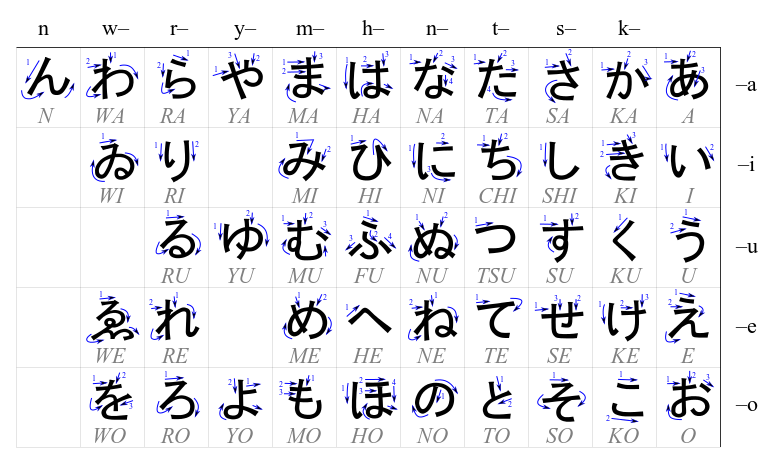
\includegraphics[scale=.2]{material/05Table_hiragana}
	\caption{Hiragana mit lat. Umschrift}
	\label{Hiragana}
\end{figure}
\end{minipage}

\end{frame}


%%%%%%%%%%%%%%%%%%%%%%%%%%%%%%%%%%
\begin{frame}
\frametitle{Phonographische Schrifttypen: Syllabisch}

%\begin{minipage}{.59\textwidth}
\begin{itemize}
	\item Korrespondenz zwischen \textbf{graphischem Zeichen} und \textbf{Silbe}
	\item Japanisch, Koreanisch, \dots
	
	%\ex. Japanisch: [Japanisch Package] für die Silbe \textipa{[ka]} (in der Silbenschrift Hiragana)

\end{itemize}
%\end{minipage}\hfill%
%%
%%
%\begin{minipage}{.4\textwidth}
	\begin{figure}
		\centering
		
		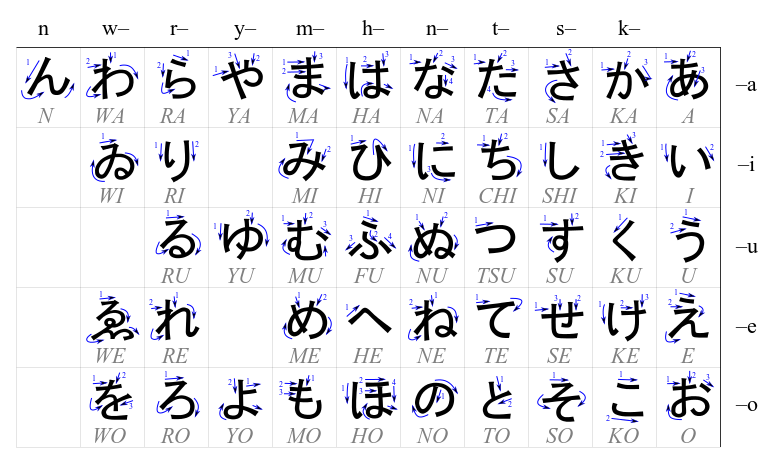
\includegraphics[scale=.25]{material/05Table_hiragana}
		\caption{Hiragana mit lat. Umschrift}
%		\label{Hiragana}
	\end{figure}
%\end{minipage}

\end{frame}


%%%%%%%%%%%%%%%%%%%%%%%%%%%%%%%%%%
\begin{frame}
\frametitle{Phonographische Schrifttypen: Alphabetisch}


\begin{itemize}

	\item Korrespondenz zwischen \textbf{graphischem Zeichen} (Buchstaben) und \textbf{Lauten}
	\item Deutsch, Russisch, Arabisch, \dots
	
	\ea Deutsch: \ab{t} für Laut \textipa{[t]}
	\z 
	
	\pause 
	
	\begin{itemize}
		\item \textbf{Konsonant-Vokal-Schrift:} \\
		enthält Grapheme für Konsonanten und Vokale
		\item Deutsch, Russisch, \dots
		
		\item \textbf{Konsonantenschrift:}\\
		enthält Grapheme (fast) nur für Konsonanten \citep[vgl.][358]{Glueck16b} 
		\item nordwestsemitische Schriftarten, Arabisch, Hebräisch, \dots
	\end{itemize}
	
	\end{itemize}

\end{frame}


%%%%%%%%%%%%%%%%%%%%%%%%%%%%%%%%%%
%%%%%%%%%%%%%%%%%%%%%%%%%%%%%%%%%%
\subsubsection{Logographische Schrifttypen}
%\iftoggle{sectoc}{
%	\frame{
%		\begin{multicols}{2}
%			\frametitle{~}
%			\tableofcontents[currentsection]
%		\end{multicols}
%	}
%}
%%%%%%%%%%%%%%%%%%%%%%%%%%%%%%%%%%

\begin{frame}
\frametitle{Logographische Schrifttypen}

\begin{itemize}
	\item Grundformen sind primär auf \textbf{bedeutungstragende} Elemente (\zB Wörter oder Morpheme) im Sprachsystem bezogen \citep[vgl.][76--77]{Duerscheid04a}. 
	
	\item Chinesisch, Teile der ägyptischen Hieroglyphen
\end{itemize}
		
\begin{minipage}{.28\textwidth}
	\begin{figure}
	\centering
	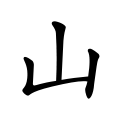
\includegraphics[scale=.45]{material/Chinesemountain-Lee-Sau-Dan}
	\caption[chinese]{Chinesisches Zeichen für `Berg'}\label{ChinBerg}
	\end{figure}
\end{minipage}\hfill%
%%
\begin{minipage}{.68\textwidth}
	\begin{figure}
	\centering
	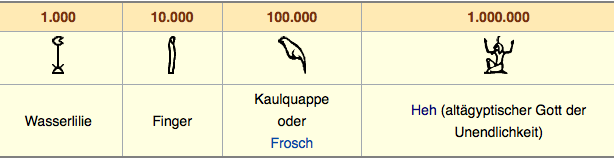
\includegraphics[scale=.37]{material/04Hieroglyphenzahlen}
	\caption[Hiero]{Hieroglyphenzahlen}\label{Hieroglyphen}
	\end{figure}
\end{minipage}
		
\end{frame}


%%%%%%%%%%%%%%%%%%%%%%%%%%%%%%%%%%
%%%%%%%%%%%%%%%%%%%%%%%%%%%%%%%%%%
\subsubsection{Fazit: Schrifttypen \& -systeme}
%\iftoggle{sectoc}{
%	\frame{
%		\begin{multicols}{2}
%			\frametitle{~}
%			\tableofcontents[currentsection]
%		\end{multicols}
%	}
%}
%%%%%%%%%%%%%%%%%%%%%%%%%%%%%%%%%%

\begin{frame}
\frametitle{Fazit: Schrifttypen \& -systeme}

\begin{itemize}
	\item Vorteil von \textbf{phonographischen} Schriftsystemen:
	
	\begin{itemize}
		\item große Menge von Wörtern mit \textbf{eher kleinem Inventar von Zeichen} (20--30) darstellbar
	\end{itemize}
	
	\item \textbf{Logographische Schrifttypen} benötigen sehr viele Zeichen.
	
	\begin{itemize}
		\item Das chinesische Schriftsystem besteht aus ungefähr 87\,000 Zeichen,\\
                  von denen zwischen 3\,000 und 5\,000 für den Alltag benötigt werden.
	\end{itemize}
	
\pause 	

	\item Vorteil von \textbf{logographischen} Schriftsystemen:
	\begin{itemize}
		\item Sie können auch von Lesern anderer Dialekte \textbf{relativ leicht dekodiert} werden.
	\end{itemize}	
\end{itemize}
\end{frame}


%%%%%%%%%%%%%%%%%%%%%%%%%%%%%%%%%%%%
%\begin{frame}
%\frametitle{Übersicht der Schrifttypen \& -systeme}
%
%
%\begin{figure}
%\centering
%\scalebox{.85}{
%	\begin{forest}
%		MyP edges
%		[\textbf{\alertred{Schrifttypen}}
%			[\textbf{logographischer} \\ Schrifttyp
%			[Chinesisch \\ Hieroglyphen, tier=word]
%			]
%			[\textbf{phonographischer} \\ Schrifttyp
%				[\textbf{alphabetischer} \\ Schrifttyp
%					[\textbf{Konsonant-Vokal-}\\Schriften
%						[Latein \\ Griechisch \\ Russisch, tier=word]
%					]
%					[\textbf{Konsonanten-}\\schriften
%						[Hebräisch \\ Arabisch, tier=word]
%					]
%				]
%				[\textbf{syllabischer} \\ Schrifttyp
%					[Japanisch \\ Koreanisch, tier=word, name=anchor] {
%					\node [right=of anchor]{\textbf{\alertred{Schriftsysteme}}};
%					}
%				]
%			]
%		]
%	\end{forest}
%}
%\end{figure}
%
%\end{frame}
%
%
%%%%%%%%%%%%%%%%%%%%%%%%%%%%%%%%%%
%%%%%%%%%%%%%%%%%%%%%%%%%%%%%%%%%%
\subsubsection{Tiefe \vs flache Systeme}
%\iftoggle{sectoc}{
%	\frame{
%		\begin{multicols}{2}
%			\frametitle{~}
%			\tableofcontents[currentsection]
%		\end{multicols}
%	}
%}
%%%%%%%%%%%%%%%%%%%%%%%%%%%%%%%%%%

\begin{frame}
\frametitle{Tiefe vs.\ flache Systeme}

\begin{itemize}
	\item trotz phonographischer/""alphabetischer Schriftsysteme \ras\\
              sehr verschiedene Schreibung in den unterschiedlichen Sprachen

	\item unterschiedliche \textbf{graphematische (/orthographische) Prinzipien},\\
          die den unterschiedlichen Schreibungen zugrunde liegen

	\item Selten 1-zu-1-Korrespondenz zwischen Phonemen und Graphemen
	
	\begin{itemize}
		\item \textbf{tiefes System}\\ 
		\vs
		\item \textbf{flaches System}
	\end{itemize}
\end{itemize}
\end{frame}


%%%%%%%%%%%%%%%%%%%%%%%%%%%%%%%%%%
\begin{frame}
\frametitle{Tiefe vs.\ flache Systeme}
\begin{itemize}
	
	\item \textbf{flaches System:}

	\begin{itemize}
		
		\item sehr gute 1-zu-1-Abbildung von Phonemen und Graphemen
		
		\item \textbf{Türkisch}
		
		\begin{itemize}
			
			\item 1928: Ersetzung der arabischen Schrift durch die lateinische Schrift
			
			\item besonders gute Phonem-Graphem-Abbildung
		\end{itemize}
	\end{itemize}

\pause 

	\item \textbf{tiefes System:}

\begin{itemize}

	\item Abbildung von Phonemen auf Graphemen, aber mit Einschränkung

	\item \textbf{Englisch} oder \textbf{Französisch}
	
	\begin{itemize}
		\item nicht häufig \textbf{reformiert} \ras starke Abweichung von Aussprache und Schriftform

		\item Englisch: \textbf{altes} und \textbf{gewachsenes} System mit sehr verschiedenen \textbf{Dialekten} in unterschiedlichen Ländern

		\item schriftliche Verständigung zwischen den Varietäten ist nur gewährleistet,\\
		wenn die Phonem-Graphem-Korrespondenz nicht streng durchgezogen wird.
	\end{itemize}
\end{itemize}
\end{itemize}

\end{frame}


%%%%%%%%%%%%%%%%%%%%%%%%%%%%%%%%%%
\begin{frame}
\frametitle{Tiefe vs.\ flache Systeme}


	\ea Türkisch: \\
	\ab{dükkan} für \textipa{[dYkkan]}
	
	\ex Spanisch: \\
	\ab{negocio} für \textipa{[negoTio]}
	
	\ex Englisch: \\
	\ab{business} für \textipa{[bIzn@z]}
	
	\ex Französisch: \\
	\ab{boutique} für \textipa{[butik]}
	\z 
	
\pause	
	
	\ea English: \ab{gh o ti} für \ab{fish} 

\pause  
	
	(\ab{gh} wie in \ab{enou\alertred{gh}}, \ab{o} wie in \ab{w\alertred{o}men}, \ab{ti} wie in \ab{na\alertred{ti}on}
	\z 

\end{frame}


%%%%%%%%%%%%%%%%%%%%%%%%%%%%%%%%%%
\begin{frame}
\frametitle{Tiefe vs.\ flache Systeme}


\begin{figure}
\centering
	
\includegraphics[scale=.3]{material/04GraphEnglischPGK}
	\caption{Englisch und PGK}\label{grammarlycard}
%{https://www.facebook.com/grammarly/photos/a.158139670871698.33824.139729956046003/942699349082389/; Autor: Grammarly; Stand: 05.12.16}
\end{figure}

\end{frame}


%%%%%%%%%%%%%%%%%%%%%%%%%%%%%%%%%%
%%%%%%%%%%%%%%%%%%%%%%%%%%%%%%%%%%
\subsection{Graphematische Prinzipien}

%% MyP: Contents
\iftoggle{sectoc}{
	\frame{
		%\begin{multicols}{2}
		\frametitle{~}
		\tableofcontents[currentsubsection, subsubsectionstyle=hide]
		%\end{multicols}
	}
}

%% StM: Contents
\iftoggle{gliederung}{
	
	\outline{
		\begin{itemize}
			
			\item Einführung
			\item Graph, Graphem, Allograph
			\item Graphematik \vs Orthographie
			\item Schrifttypen \& -systeme
			%%Phonographische Schrifttypen
			%%Logographische Schrifttypen
			%%Fazit: Schrifttypen & -systeme
			%%Tiefe vs. flache Systeme
			\item \blaubf{Graphematische Prinzipien}
			%%Phonographisches Prinzip
			%%Silbisches Prinzip
			%%Morphologisches Prinzip
			%%Differenzierung homophoner Formen
			%%Etymologische Schreibung
			%%Ästhetische Schreibung
			%%Syntaktische Schreibung
			\item Hausaufgabe
			
		\end{itemize}
	}
}


%%%%%%%%%%%%%%%%%%%%%%%%%%%%%%%%%%
\begin{frame}
\frametitle{Graphematische Prinzipien/Tendenzen}

\begin{itemize}
	\item \textbf{Schrifttyp} bedingt das graphematische System.
	\item Daraus ergibt sich die \textbf{Gewichtung} (oder Vorhandensein) weiterer
Prinzipien:

	\begin{itemize}
		\item Deutsch: alphabetischer Schrifttyp \ras Abbildung von Phonemen mit Graphemen

		\item Abbildung von Phonemen auf Grapheme $=$ \\
		\textbf{Phonem-Graphem-Korrespondenz} (PGK)
		
		\item Weitere Prinzipien:
		
		\begin{itemize}
			\item \textbf{Wortebene}:\\
			regelhafte Markierung von Silben, Morphemen und Bedeutungseinheiten, \dots

			\item \textbf{Satzebene}: \\
			regelhafte Groß- und Kleinschreibung, Zusammen- und Getrenntschreibung, \dots
		\end{itemize}
	
	\end{itemize}

\end{itemize}
\end{frame}


%%%%%%%%%%%%%%%%%%%%%%%%%%%%%%%%%%
\begin{frame}
\frametitle{Graphematische Prinzipien/Tendenzen}

\begin{itemize}
	\item Das graphematische System des Deutschen wird von diesen
	\textbf{meist regelhaften Prinzipien bestimmt} und dementsprechend
	(anschließend) auch \textbf{normiert}, sodass es nur eine einzige
	mögliche (normierte) Schreibung für ein Wort gibt.
	
	\begin{itemize}
		\item Erkundung und Erklärung von Regelmäßigkeiten des Systems \\
		\ras \textbf{graphematische Herangehensweise}
		
		\item Anwendung der Regelmäßigkeiten mit einem präskriptiven,
		normativen Charakter \\
		\ras \textbf{orthographische Herangehensweise}
	\end{itemize}
\end{itemize}

\end{frame}


%%%%%%%%%%%%%%%%%%%%%%%%%%%%%%%%%%
\begin{frame}
\frametitle{Graphematische Prinzipien/Tendenzen}

\begin{itemize}
	\item Graphematische/Orthographische \gqq{Prinzipien/Tendenzen}:
	
	\begin{itemize}
		\item Phonographisches Prinzip (nach Phonem-Graphem-Korrespondenzen)

		\item Silbisches Prinzip

		\item Morphologisches Prinzip (auch Prinzip der Morphemkonstanz)

		\item Differenzierung homophoner Formen

		\item Etymologische Schreibung

		\item Ästhetische Schreibung 

		\item Syntaktische Schreibung 
	\end{itemize}

\item  Es handelt sich eher um \textbf{Tendenzen} (weniger um Prinzipien), \\
weil sie nicht immer \textbf{regelhaft} sind.

\end{itemize}


\end{frame}


%%%%%%%%%%%%%%%%%%%%%%%%%%%%%%%%%%
%%%%%%%%%%%%%%%%%%%%%%%%%%%%%%%%%%
\subsubsection{Phonographisches Prinzip}
%\iftoggle{sectoc}{
%	\frame{
%		\begin{multicols}{2}
%			\frametitle{~}
%			\tableofcontents[currentsection]
%		\end{multicols}
%	}
%}
%%%%%%%%%%%%%%%%%%%%%%%%%%%%%%%%%%

\begin{frame}
\frametitle{Phonographisches Prinzip}

\begin{itemize}
	\item Phoneme werden mit Graphemen wiedergegeben.
	\item \textbf{Phonem-Graphem-Korrespondenzen} (auch PGK-Regeln)

\pause	

	\item Abbildung von \textbf{Lauten} (Phonen) in Form von Buchstaben (Phon--Graphem)\\ 
	\vs
	\item Abbildung von \textbf{abstrakten, regulären Lautmengen} in
Form von Buchstaben (Phonem--Graphem)

\end{itemize}

\end{frame}


%%%%%%%%%%%%%%%%%%%%%%%%%%%%%%%%%%
\begin{frame}
\frametitle{Phonographisches Prinzip}

\begin{itemize}
	
	\item \textbf{Pro}: Phon $\leftrightarrow$ Graphem

	\begin{itemize}
		\item sehr genaue Abbildung
		\item einfach für den Leser
	\end{itemize}

\pause 
	
	\item \textbf{Contra}: Phon $\leftrightarrow$ Graphem
	
	\begin{itemize}
		\item größeres Inventar an Buchstaben nötig
		
		\ea Unterschiedliche Buchstaben(-kombinationen) für \ab{ch}\\
		\zB in \ab{i\alertred{ch}} und \ab{Bu\alertred{ch}}
		\z 

\pause 		

		\item Variabilität der Aussprache in einem Dialekt und in unterschiedlichen Dialekten
		
		\ea Unterschiedliche Schreibung von \ab{Sport},\\
		\zB \ab{Spo\alertred{R}t}, \ab{Spo\alertred{r}t}, \ab{Spo\alertred{a}t}, \ab{Spo\alertred{ch}t}
		\z 

\pause 
		
		\item \gqq{Verwandtschaft} zwischen Wortformen nicht mehr erkennbar
		
		\ea Unterschiedliche Schreibung von \ab{r}\\
		\zB in \ab{hö\alertred{a}t} \vs \ab{hö\alertred{r}en}
		\z 
	\end{itemize}
\end{itemize}

\end{frame}


%%%%%%%%%%%%%%%%%%%%%%%%%%%%%%%%%%
\begin{frame}
\frametitle{Phonographisches Prinzip}

\begin{itemize}
	\item \textbf{Pro} Phonem $\leftrightarrow$ Graphem
	
	\begin{itemize}
		\item einheitliche Wiedergabe von komplementärer, freier und regionaler \textbf{Allophonie}

		\item \textbf{Definition von Graphem} als kleinste bedeutungsunterscheidende Einheit eines Schriftsystems (parallel zu Phonem)
	\end{itemize}

\pause 
	
	\item \textbf{Contra} Phonem $\leftrightarrow$ Graphem
	
	\begin{itemize}
		\item etwas komplizierter \textbf{für den Leser}
		
		\ea Wann wird ein \ab{ch} wie in \ab{i\alertred{ch}} oder wie in \ab{Bu\alertred{ch}} ausgesprochen?
		\z 
		
		\item ABER: Dafür \textbf{reduziert} sich der \textbf{Lernaufwand} bzgl.\ der Menge von zu lernenden Buchstaben.	
	\end{itemize}
\end{itemize}

\end{frame}


%%%%%%%%%%%%%%%%%%%%%%%%%%%%%%%%%%
\begin{frame}
\frametitle{PGK: Konsonanten}

\begin{table}
\centering
\scalebox{0.8}{
\begin{tabular}{l l l | l l l}
\textbf{Phonem} & \textbf{einige mögliche} & \textbf{Graphem} & \textbf{Phonem} & \textbf{einige mögliche } & \textbf{Graphem} \\
& \textbf{Allophone} & & & \textbf{Allophone} & \\ 
\textipa{/p/} & \textipa{[p], [p\super h]} & \ab{p} & \textipa{/\c{c}/} & \textipa{[\c{c}], [x]} & \ab{ch} \\
\textipa{/t/} & \textipa{[t], [t\super h]} & \ab{t} & \textipa{/v/} & \textipa{[v]} & \ab{w} \\
\textipa{/k/} & \textipa{[k], [k\super h]} & \ab{k} & \textipa{/j/} & \textipa{[j]} & \ab{j} \\
\textipa{/b/} & \textipa{[b], [p]} & \ab{b} & \textipa{/h/} & \textipa{[h]} & \ab{h} \\
\textipa{/d/} & \textipa{[d], [t]} & \ab{d} & \textipa{/m/} & \textipa{[m]} & \ab{m} \\
\textipa{/g/} & \textipa{[g], [k]} & \ab{g} & \textipa{/n/} & \textipa{[n]} & \ab{n} \\
\textipa{/k/+/v/} & [\textsubplus{k}]\textipa{[v]} & \ab{qu} & \textipa{/l/} & \textipa{[l]} & \ab{l} \\
\textipa{/f/} & \textipa{[f]} & \ab{f} & /\textscr{}/ & [\textscr{}], \textipa{[K], [r], [5]} & \ab{r} \\
\textipa{/s/} & \textipa{[s]} & \ab{ß} & \textipa{/\t{pf}/} & \textipa{[\t{pf}]} & \ab{pf} \\
\textipa{/s/} & \textipa{[s]} & \ab{s} &   &   &   \\
\textipa{/z/} & \textipa{[z], [s]} & \ab{s} & \textipa{/\t{ts}/} & \textipa{[\t{ts}]} & \ab{z} \\
\textipa{/S/} & \textipa{[S]} & \ab{sch} & \textipa{/\t{tS}/} & \textipa{[\t{tS}]} & \ab{tsch} \\
	
\end{tabular} 
}
%\caption{Phonem-Graphem-Korrespondenzen für Konsonanten}
\end{table}

\pause 

\ea \textipa{/s/}, \textipa{[s]}, \ab{\alertred{ß}} (zwischensilbisch nach XX im Nukleus): au\ab{\alertred{ß}}er, Mu\ab{\alertred{ß}}e

\ex \textipa{/s/}, \textipa{[s]}, \ab{\alertred{s}} (im Auslaut): da\ab{\alertred{s}}, e\ab{\alertred{s}}

\ex \textipa{/z/}, \textipa{[z], [s]}, \ab{\alertred{s}}: \ab{\alertred{s}}ieh\ab{\alertred{s}}t  
\z 


\end{frame}


%%%%%%%%%%%%%%%%%%%%%%%%%%%%%%%%%%%
\begin{frame}
\frametitle{PGK: Vokale}


\begin{table}
\centering
%\scalebox{0.8}{
\begin{tabular}{l l | l l}
	\textbf{Vokalphonem} & \textbf{Graphem} & \textbf{Vokalphonem} & \textbf{Graphem} \\
	\textbf{(lang und gespannt)} & & \textbf{(kurz und ungespannt)} & \\
	\textipa{/i:/} & \ab{ie} & \textipa{/I/} & \ab{i} \\
	\textipa{/y:/} & \ab{ü} & \textipa{/Y/} & \ab{ü} \\
	\textipa{/e:/} & \ab{e} & & \\
	\textipa{/E:/} & \ab{ä} & \textipa {/E/} & \ab{e} \\
	& & \textipa{/@/} & \ab{e} \\
	\textipa{/\o:/} & \ab{ö} & 	\textipa{/\oe/} & \ab{ö} \\
	\textipa{/A:/} & \ab{a} & \textipa{/a/} & \ab{a} \\
	\textipa{/o:/} & \ab{o} & \textipa{/O/} & \ab{o} \\ 
	\textipa{/u:/} & \ab{u} & \textipa{/U/} & \ab{u} \\
\end{tabular}
%}
%\caption{Phonem-Graphem-Korrespondenzen für Vokale}
\end{table}

\end{frame}


%%%%%%%%%%%%%%%%%%%%%%%%%%%%%%%%%%
\begin{frame}
\frametitle{PGK: Diphthonge}

\begin{table}
	\centering
%	\scalebox{0.8}{
	\begin{tabular}{l l}
		\textbf{Diphthong} & \textbf{Digraph} \\
		\textipa{/\t{aI}/} & \ab{ei} \\
		\textipa{/\t{aU}/} & \ab{au} \\
		\textipa{/\t{O}I/} & \ab{eu} \\	
	\end{tabular}		
%	}
%\caption{Phonem-Graphem-Korrespondenzen für Diphthonge}
\end{table}

\begin{description}
	\item[Digraph] Graphem aus zwei Buchstaben 
	
	\item[Trigraph] Graphem aus drei Buchstaben
\end{description}

\end{frame}


%%%%%%%%%%%%%%%%%%%%%%%%%%%%%%%%%%
\begin{frame}
\frametitle{Übung}

\begin{itemize}
	\item Geben Sie 10 Wörter an, die phonographisch geschrieben werden.
	\item Wie würden Sie die folgenden Wörter phonographisch schreiben?

	\ea\label{ex:04aphilo}
		\ea Philosophie
		\ex Balkon
		\ex Creme
		\ex Mutter
		\ex Streithahn
		\z
	\z
	
\end{itemize}
	
\end{frame}


%%%%%%%%%%%%%%%%%%%%%%%%%%%%%%%%%
%%%%%%%%%%%%%%%%%%%%%%%%%%%%%%%%%
\iftoggle{ue-loesung}{
	%%%%%%%%%%%%%%%%%%%%%%%%%%%%%%%%%%
%% UE 1 - 04a Graphematik
%%%%%%%%%%%%%%%%%%%%%%%%%%%%%%%%%%

\begin{frame}
\frametitle{Übung -- Lösung}

\begin{itemize}
	\item Geben Sie 10 Wörter an, die phonographisch geschrieben werden.
	
		\begin{description}
			\item[\alertgreen{\textbf{Beispiele:}}] \alertgreen{Beurteilung, schön, Gabel, suchen, Macht, Lager, kurz, niesen, Zopf, Gewerkschaft}
		\end{description}
	
	\item Wie würden Sie die folgenden Wörter phonographisch schreiben?
		
	\begin{exe}
		\exr{ex:04aphilo}
	\settowidth\jamwidth{XXXXXXXXXXXXXXXXXXXXXXXXXXXXX}
		\begin{xlist}
			\ex Philosophie \loesung{2}{\ab{filosofie}}
			\ex Balkon \loesung{3}{\ab{balkong}}
			\ex Creme \loesung{4}{\ab{krem} oder \ab{kreme}}
			\ex Mutter \loesung{5}{\ab{muter}}
			\ex Streithahn \loesung{6}{\ab{schtreithan}}
		\end{xlist}
	\end{exe}
		

\end{itemize}

\end{frame}


}

%%%%%%%%%%%%%%%%%%%%%%%%%%%%%%%%%%
\begin{frame}
\frametitle{Übung}

\begin{itemize}	
	\item Versuchen Sie, graphematische Regularitäten und Prinzipien zu finden, die die Unterscheidung "`lang \vs kurz"' bei Vokalen anzeigen. Gibt es Ausnahmen?
	
	\ea\label{ex:04amutter}
	
	\begin{multicols}{2}
		\ea Mutter
		\ex Mehl
		\ex See
		\ex Nase
		\ex dehnen
		\ex gehen
		\ex Bier
		\ex Moor
		\ex an
		\ex zum
		\ex Mann
		\ex man
		\ex Herbst
		\ex Laub
		\ex sehr
		\ex Bohrer
		\z
	\end{multicols}
	
	\z
	
\end{itemize}

\end{frame}


%%%%%%%%%%%%%%%%%%%%%%%%%%%%%%%%%%
%%%%%%%%%%%%%%%%%%%%%%%%%%%%%%%%%%
\iftoggle{ue-loesung}{
	%%%%%%%%%%%%%%%%%%%%%%%%%%%%%%%%%%
%% UE 2 - 04a Graphematik
%%%%%%%%%%%%%%%%%%%%%%%%%%%%%%%%%%

\begin{frame}
\frametitle{Übung -- Lösung}

\begin{itemize}	
	\item Versuchen Sie, graphematische Regularitäten und Prinzipien zu finden, die die Unterscheidung lang \vs kurz bei Vokalen anzeigen. Gibt es Ausnahmen?\\
	
%	\vspace{-.3cm}
	
	\begin{exe}
		\exr{ex:04amutter}
		\begin{xlist}
			\begin{multicols}{4}
				\ex Mutter
				\ex Mehl
				\ex See
				\ex Nase
				\ex dehnen
				\ex gehen
				\ex Bier
				\ex Moor
				\ex rot
				\ex zum
				\ex Mann
				\ex man
				\ex Herbst
				\ex Laub
				\ex sehr
				\ex Bohrer
			\end{multicols}
		\end{xlist}
	\end{exe}
	
\end{itemize}

%\vspace{-.3cm}


\begin{multicols}{2}
\begin{itemize}
\item[\alertgreen{--}] \alertgreen{Diphthonge: lang (n.)}
\item[\alertgreen{--}] \alertgreen{Doppelvokale: lang (c., h.), Sonderfall bei \ab{i}: \ab{ie} (g.)}
\item[\alertgreen{--}] \alertgreen{vor Dehnungs-h: lang (b., e., o., p.)}
\item[\alertgreen{--}] \alertgreen{vor Doppelkonsonant: kurz (a., k.)}
\item[\alertgreen{--}] \alertgreen{vor Konsonantencluster: kurz (m.)}
\item[\alertgreen{--}] \alertgreen{offene Schreibsilben: lang bei Hauptbetonung (d., f.),
\\sonst kurz (d.)}
\item[\alertgreen{--}] \alertgreen{einfach geschlossene Schreibsilben: uneindeutig bei Hauptbetonung\\(i., j., l.), sonst kurz (a., e., f., p.)}
\end{itemize}
\end{multicols}

\end{frame}


}

%%%%%%%%%%%%%%%%%%%%%%%%%%%%%%%%%%
%%%%%%%%%%%%%%%%%%%%%%%%%%%%%%%%%%
\subsubsection{Silbisches Prinzip}
%\frame{
%\frametitle{~}
%	\tableofcontents[currentsection]
%}


%%%%%%%%%%%%%%%%%%%%%%%%%%%%%%%%%%
\begin{frame}
\frametitle{Silbisches Prinzip}

\begin{itemize}
	\item auch durch die Lautstruktur zu begründen, aber nicht reine Phonem-Graphem-Beziehungen \ras Bezug auf Vokalqualität/-quantität
	
	\item In der Graphematik wird (analog zur Silbe in der Phonologie) eine Silbe angenommen \citep[vgl.][]{Fuhrhop08a}:
	
	\begin{itemize}
		\item[]
		\item \textbf{Anfangsrand}: Konsonant(en),\\
		leerer Anfangsrand: \textbf{nackte} Silbe\\
		besetzter Anfangsrand: \textbf{bedeckte} Silbe
		\item[]
		\item \textbf{Silbenkern}: Vokal oder Diphthong
		\item[]
		\item \textbf{Endrand}: Konsonant(en)\\
		leerer Endrand: \textbf{offene} Silbe\\
		besetzter Endrand: \textbf{geschlossene} Silbe
	\end{itemize}
\end{itemize}

\end{frame}


%%%%%%%%%%%%%%%%%%%%%%%%%%%%%%%%%%
\begin{frame}
\frametitle{Silbisches Prinzip: (Un-)Gespanntheit}

\begin{itemize}
	\item Vokalqualität (\dash Gespanntheit) und -quantität (\dash Länge) wird phonographisch nicht eindeutig abgebildet (s.\ PGK für Vokale), aber es gibt \textbf{Tendenzen auf Silbenebene}.
	\item[]
	\item für \textbf{morphologisch einfache Wörter} 
	
	\begin{itemize}
		\item offene Silbe \ras \textbf{gespannter} Vokal: 
		
		\ea \ab{Kl\alertred{o}}, \ab{s\alertred{o}} (weitere Markierung: \ab{Se\alertred{e}}, \ab{Re\alertred{h}})
		\z
		
		\item geschlossene Silbe mit komplexem Endrand \ras \textbf{ungespannter} Vokal: 
		
		\ea
		\ab{Stru\alertred{mpf}}, \ab{Bi\alertred{ld}}
		\z
		
		\item wenige \textbf{Ausnahmen} \citep[vgl.][15]{Fuhrhop09a}: 
		
		\ea
		\ab{Mo\alertred{nd}}, \ab{Ke\alertred{ks}}, \ab{O\alertred{bst}}
		\z
		
	\end{itemize}
\end{itemize}
\end{frame}


%%%%%%%%%%%%%%%%%%%%%%%%%%%%%%%%%%
\begin{frame}
\frametitle{Silbisches Prinzip: (Un-)Gespanntheit}

\begin{itemize}
	\item für \textbf{morphologisch einfache Wörter}
	
	\begin{itemize}
		\item geschlossene Silbe mit einfachem Endrand \ras \textbf{gespannter} oder \textbf{ungespannter} Vokal möglich:
		
		\ea \ab{B\alertred{ee}t} -- \ab{B\alertred{e}tt}, \ab{B\alertred{a}hn} -- \ab{B\alertred{a}nn}
		\z

\pause 
		
		\item \textbf{zusätzliche Markierungen} möglich, aber nicht immer markiert: 
		
		\ea 
			\ea ungespannt/kurz: \ab{a\alertred{n}}, \ab{bi\alertred{s}}
		
			\ex gespannt/lang: \ab{ro\alertred{t}}, \ab{Hu\alertred{t}}
			\z
		\z 
	\end{itemize}
\end{itemize}

\end{frame}


%%%%%%%%%%%%%%%%%%%%%%%%%%%%%%%%%%
\begin{frame}
\frametitle{Silbisches Prinzip: Markierungen der (Un-)Gespanntheit}

	\begin{itemize} 
		\item Markierung der \textbf{Gespanntheit} durch \textbf{Verdoppelung des Vokals} \ab{aa}, \ab{ee}, \ab{oo} oder \ab{\textbf{ie}} 
		
		\ea \ab{B\alertred{ee}t}, \ab{S\alertred{aa}l}, \ab{B\alertred{oo}t}, \ab{T\alertred{ie}r}, \ab{M\alertred{eh}l}
		\z

		\begin{itemize}
			\item lediglich \ab{ee} findet sich auch in offenen Silben, vermutlich weil \ab{e} sowohl für /\textschwa{}/ als auch für \textipa{/e/} steht.
		
		\ea \ab{S\alertred{ee}}, \ab{Arm\alertred{ee}}, \ab{Klisch\alertred{ee}}, \ab{All\alertred{ee}}%, \ab{\textbf{Orchidee}}
		\z
		\end{itemize}
	
		\item vor \textbf{Sonoranten}: Markierung der \textbf{Gespanntheit} durch ein \ab{\textbf{h}} \textbf{nach dem Vokal} (Dehnungs-h) 
		
		\ea \ab{Me\alertred{h}l}, \ab{Bo\alertred{h}rer}, \ab{Ba\alertred{h}n}
		\z
	\end{itemize}

\end{frame}


%%%%%%%%%%%%%%%%%%%%%%%%%%%%%%%%%%
\begin{frame}
\frametitle{Silbisches Prinzip: Ungespanntheit \& Silbengelenk}

\begin{itemize}
	\item \textbf{Ungespanntheit} wird \ua durch die \textbf{Verdopplung des Folgekonsonanten} (Geminatenschreibung) angezeigt, in zweisilbigen Wörtern sind diese Konsonanten dann \textbf{ambisyllabisch} (\dash Silbengelenk): 


\ea \ab{E\alertred{bb}e}, \ab{A\alertred{ff}e}, \ab{Kla\alertred{dd}e}
\z

	\item Achtung: Im Deutschen markiert die \textbf{Konsonantenverdopplung} primär ein \textbf{Silbengelenk}. Silbenkgelenke kommen \textbf{nach kurzen ungespannten Vokalen} vor.
	
	\item In Fällen wie (\ref{ex:GraphGelenk1}) korreliert die Geminatenschreibung mit dem morphologischen Prinzip, vgl.\ (\ref{ex:GraphGelenk2}).

	\ea 
	\ea\label{ex:GraphGelenk1} \ab{Fa\alertred{ll}}, \ab{Ma\alertred{nn}}
	\ex\label{ex:GraphGelenk2} \ab{Fä\alertred{ll}e}, \ab{Mä\alertred{nn}er}
	\z
	\z 
\end{itemize}
\end{frame}


%%%%%%%%%%%%%%%%%%%%%%%%%%%%%%%%%%
\begin{frame}
\frametitle{Silbisches Prinzip: silbentrennendes \ab{h}}
	
	\begin{itemize}
	\item zwischen zwei \textbf{vokalischen Silbenkernen} zur \textbf{Markierung der Zweisilbigkeit}
	
	
	\eal
	\ex \ab{ge-\alertred{h}en}
	\ex \ab{Ru-\alertred{h}e}
	\ex \ab{Mü-\alertred{h}e}
	\zl

\pause
	
	\item besonders häufig in Verben
	\eal
	\ex \ab{se\alertred{h}en}
	\ex \ab{ste\alertred{h}en}
	\zl
	
\pause
	
	\item nicht nach Diphthongen, außer \ab{ei}
	\eal
	\ex \ab{h\alertblue{au}en}
	\ex \ab{sch\alertblue{au}en}
	\ex \ab{lei\alertred{h}en}
	\ex \ab{verzei\alertred{h}en}
	\ex \ab{schr\alertblue{ei}en}
	\zl

	\end{itemize}

\end{frame}


%%%%%%%%%%%%%%%%%%%%%%%%%%%%%%%%%%
%%%%%%%%%%%%%%%%%%%%%%%%%%%%%%%%%%
\subsubsection{Morphologisches Prinzip}
%\iftoggle{sectoc}{
%	\frame{
%		\begin{multicols}{2}
%			\frametitle{~}
%			\tableofcontents[currentsection]
%		\end{multicols}
%	}
%}
%%%%%%%%%%%%%%%%%%%%%%%%%%%%%%%%%%

\begin{frame}
\frametitle{Morphologisches Prinzip}

\begin{itemize}
	\item auch Prinzip der Morphemkonstanz, Stammschreibungsprinzip, Verwandtschaftsprinzip
	
	\item Wörter oder Wortformen, die in einer \textbf{morphologischen Beziehung} stehen, werden ähnlich oder gleich geschrieben.
	
	\eal
	\ex \ab{\alertred{A}pfel} -- \ab{\alertred{Ä}pfel}, nicht \ab{Epfel}
	\ex \ab{Hun\alertred{d}} -- \ab{Hun\alertred{d}e}, nicht \ab{Hunt}
	\ex \ab{gro\alertred{ß}} -- \ab{grö\alertred{ß}er}, nicht \ab{gros}
	\ex \ab{B\alertred{a}\alertblue{ll}} -- \ab{B\alertred{ä}\alertblue{ll}e}, nicht \ab{Bal} und \ab{Belle}
	\zl

	\item Bei einigen (wenigen) Wörtern sind zwei Schreibungen zugelassen, um die Verwandtschaft zu verschiedenen Derivaten des gleichen Morphems zu kennzeichnen.
	
	\ea 
	\ea \ab{aufw\alertred{ä}ndig} zu \ab{Aufw\alertred{a}nd}
	\ex \ab{aufw\alertred{e}ndig} zu \ab{aufw\alertred{e}nden}
	\z
	\z 
\end{itemize}

\end{frame}


%%%%%%%%%%%%%%%%%%%%%%%%%%%%%%%%%%
%%%%%%%%%%%%%%%%%%%%%%%%%%%%%%%%%%
%\subsubsection{Übung}
%\frame{
%\frametitle{~}
%	\tableofcontents[currentsection]
%}

%%%%%%%%%%%%%%%%%%%%%%%%%%%%%%%%%%
\begin{frame}
\frametitle{Übung}

\begin{itemize}
	\item Warum schreibt man \ab{dehnen} mit \ab{h}, obwohl das erste \ab{e} in einer offenen Silbe steht und daher nach silbischen Prinzipien sowieso lang gesprochen werden müsste?
	\item[]
	\item Warum schreibt man \ab{mann} und \ab{ball}, obwohl nach silbischen Prinzipien die Geminate einen ambisyllabischen Konsonanten anzeigt?
	\item[]
	\item Warum sind die Wörter \ab{(du) ziehst}, \ab{säubern} und \ab{(er) fällt} Beispiele für morphologisches Schreiben?
	\item[]
	\item Wie hätte eine Person, die \ab{Rad} und \ab{König} als Beispiele für das morphologische Prinzip anführt, \gqq{phonographisches Schreiben} verstanden?
\end{itemize}


\end{frame}


%%%%%%%%%%%%%%%%%%%%%%%%%%%%%%%%%%
%%%%%%%%%%%%%%%%%%%%%%%%%%%%%%%%%%
\iftoggle{ue-loesung}{
	%%%%%%%%%%%%%%%%%%%%%%%%%%%%%%%%%%
%% UE 3 - 04a Graphematik
%%%%%%%%%%%%%%%%%%%%%%%%%%%%%%%%%%

\begin{frame}
\frametitle{Übung -- Lösung}

\begin{itemize}
	\item Warum schreibt man \ab{dehnen} mit \ab{h}, obwohl das erste \ab{e} in einer offenen Silbe steht und daher nach silbischen Prinzipien sowieso lang gesprochen werden müsste?
		\item[] \alertgreen{Morphemkonstanz, da bei Flexionsformen wie \ab{dehnst} geschlossene Silbe}
	\item Warum schreibt man \ab{mann} und \ab{ball}, obwohl nach silbischen Prinzipien die Geminate einen ambisyllabischen Konsonanten anzeigt?
		\item<2->[] \alertgreen{Morphemkonstanz, da Pluralform Silbengelenk hat}
	\end{itemize}


\end{frame}


%%%%%%%%%%%%%%%%%%%%%%%%%%
\begin{frame}
\frametitle{Übung -- Lösung}

\begin{itemize}
	\item Warum sind die Wörter \ab{(du) ziehst}, \ab{säubern} und \ab{(er) fällt} Beispiele für morphologisches Schreiben?
		\item<2->[] \alertgreen{\ab{h} im Infinitiv silbentrennend, Singular-Flexionsformen sind jedoch einsilbig;}
		\item<3->[] \alertgreen{\ab{ä} zeigt die Verwandschaft zu \ab{sauber}: laut PGK schriebe man \textipa{[O\texttoptiebar{}I]} \ab{eu};}
		\item<4->[] \alertgreen{Konsonantenverdopplung wegen Silbengelenk im Infinitiv, Singular-Flexionsformen sind jedoch einsilbig,\\ \ab{ä} wegen \ab{a} im Infinitiv: \textipa{[E]} wäre nach PGK \ab{e}}
	\item Wie hätte eine Person, die \ab{Rad} und \ab{König} als Beispiele für das morphologische Prinzip anführt, \gqq{phonographisches Schreiben} verstanden?
		\item<5->[] \alertgreen{Verschriftlichung der \emph{phonetischen} (richtig wäre: \emph{phonologische}) Repräsentation}
\end{itemize}


\end{frame}


}

%%%%%%%%%%%%%%%%%%%%%%%%%%%%%%%%%%
%%%%%%%%%%%%%%%%%%%%%%%%%%%%%%%%%%
\subsubsection{Differenzierung homophoner Formen}
%\frame{
%\frametitle{~}
%	\tableofcontents[currentsection]
%}


%%%%%%%%%%%%%%%%%%%%%%%%%%%%%%%%%%
\begin{frame}
\frametitle{Differenzierung homophoner Formen}

\begin{itemize}
	
	\item auch Homonym(ie)differenzierung, -vermeidung
	
	\item \textbf{Gleichlautende Wörter} mit \textbf{unterschiedlicher Bedeutung} werden orthographisch unterschiedlich repräsentiert.
	
	\ea L\alertred{ei}b -- L\alertred{ai}b; S\alertred{ei}te -- S\alertred{ai}te; L\alertred{ie}d -- (Augen)L\alertred{i}d
	\z
	
	\item Aber:
	
	\ea Kiefer -- Kiefer; Bremse -- Bremse; Ton -- Ton
	\z
	
	\item Möglichkeiten zur Homophonendifferenzierung werden also keineswegs konsequent ausgenutzt.
\end{itemize}

\end{frame}


%%%%%%%%%%%%%%%%%%%%%%%%%%%%%%%%%%
%%%%%%%%%%%%%%%%%%%%%%%%%%%%%%%%%%
\subsubsection{Etymologische Schreibung}
%\iftoggle{sectoc}{
%	\frame{
%		\begin{multicols}{2}
%			\frametitle{~}
%			\tableofcontents[currentsection]
%		\end{multicols}
%	}
%}
%%%%%%%%%%%%%%%%%%%%%%%%%%%%%%%%%%

\begin{frame}
\frametitle{Etymologische Schreibung}

\begin{itemize}
	\item Die Schreibung \gqq{\textbf{alter}} oder \textbf{entlehnter} Wörter bleibt erhalten,\\
	auch wenn sie nicht den aktuellen Schreibprinzipien entspricht.
	
	\eal
		\ex \ab{wa\alertred{nn}} statt \ab{wan} (wegen mhd. \ab{wanne})
		%% Hier ist kein Silbengelenk möglich!
		
		\ex \ab{\alertred{C}rem\alertred{e}} statt \ab{Krem}
		
		\ex \ab{Restaurant} statt \ab{Restorong}
		
		\ex \ab{Ort\alertred{h}ogra\alertred{ph}ie} oder \ab{Ort\alertred{h}ografie} statt \ab{Ortografie}
	\zl

\end{itemize}

\end{frame}


%%%%%%%%%%%%%%%%%%%%%%%%%%%%%%%%%%
%%%%%%%%%%%%%%%%%%%%%%%%%%%%%%%%%%
\subsubsection{Ästhetische Schreibung}
%\iftoggle{sectoc}{
%	\frame{
%		\begin{multicols}{2}
%			\frametitle{~}
%			\tableofcontents[currentsection]
%		\end{multicols}
%	}
%}
%%%%%%%%%%%%%%%%%%%%%%%%%%%%%%%%%%

\begin{frame}
\frametitle{Ästhetische Schreibung}

\begin{itemize}
	\item \textbf{Schreibsilben} sollten nicht zu lang und nicht zu kurz sein.
	
	\eal
	\ex \ab{\alertred{S}piel} statt \ab{Schpiel}
	\ex \ab{Schw\alertred{a}n} statt \ab{Schw\alertred{ah}n}
	\zl

\pause 
	
	\item \textbf{Verbot von Doppelschreibungen} von einigen Vokalgraphemen (\ab{i} und \ab{u} sowie Umlaute) -- teilweise bedingt durch \textbf{Verwechslungsgefahr}
	
	\ea
	\ab{ii} wie \ab{ü}; \ab{uu} wie \ab{w}
	\z
	
\pause 
		
	\item Verbot von \textbf{Doppelschreibung von Mehrgraphemen} wie
	
	\eal
		\ex \ab{ng} in \ab{Bearbeitu\alertred{ngng}en}
		\ex \ab{ch} in \ab{Bü\alertred{chch}er} 
		\ex \ab{sch} in \ab{graphi\alertred{schsch}e}
	\zl
	
\end{itemize}

\end{frame}


%%%%%%%%%%%%%%%%%%%%%%%%%%%%%%%%%%
%%%%%%%%%%%%%%%%%%%%%%%%%%%%%%%%%%
\subsubsection{Syntaktisches Prinzip}
%\iftoggle{sectoc}{
%	\frame{
%		\begin{multicols}{2}
%			\frametitle{~}
%			\tableofcontents[currentsection]
%		\end{multicols}
%	}
%}
%%%%%%%%%%%%%%%%%%%%%%%%%%%%%%%%%%

\begin{frame}
\frametitle{Syntaktisches Prinzip}

\begin{itemize}
	\item \textbf{Großschreibung für Substantive} und Substantivierungen von Adjektiven, Verben, Adverbien, Partikeln, usw. 

	\ea das \alertred{J}a, das \alertred{G}estern, das \alertred{I}ch
	\z 
	
	\item Großschreibung von \textbf{Satzanfängen} und in \textbf{Anreden}
	
	\ea \alertred{S}ie, \alertred{I}hr
	\z 

	
	\item Die Großschreibung von Substantiven gibt es nur in der deutschen und luxemburgischen Schreibung.\\
	Während der Rechtschreibreform hat man diskutiert, diese abzuschaffen.\\
	Was denken Sie: Was spräche dafür, was dagegen?

\pause 
	
	\ea Berliner Berliner berlinern berlinernd berlinisches Berlinisch.
	\z 
\end{itemize}

\end{frame}




%%%%%%%%%%%%%%%%%%%%%%%%%%%%%%%%%%
%%%%%%%%%%%%%%%%%%%%%%%%%%%%%%%%%%
%\subsection{Übungen}
%\iftoggle{sectoc}{
%	\frame{
%		\begin{multicols}{2}
%			\frametitle{~}
%			\tableofcontents[currentsection]
%		\end{multicols}
%	}
%}


%%%%%%%%%%%%%%%%%%%%%%%%%%%%%%%%%%
\begin{frame}
\frametitle{Übung}

\begin{itemize}
	\item Welche graphematischen Prinzipien (abgesehen von der phonographischen Schreibung) erklären die Schreibung der folgenden Wörter?
	
	  \ea\label{ex:04azimmer}
	  \begin{multicols}{3}
          \ea \ab{Zimmer}
          \ex \ab{Waise}
          \ex \ab{Wehen}
          \ex \ab{Ruhm}
          \ex \ab{Spaß}
          \ex \ab{Allee}
%          \ex \ab{Gras}
          \z
        \end{multicols}
      \z

	\item Welche graphematische Funktion erfüllt das \ab{h} in den folgenden Wörtern?
	
	  \ea\label{ex:04anacht}
	  \begin{multicols}{4}
          \ea \ab{Nacht}
          \ex \ab{Hilfe}
          \ex \ab{sehen}
          \ex \ab{Mehl}
          \z
        \end{multicols}
      \z
      
	\item Wie würden die folgenden Wörter in phonographischer Schreibung aussehen? Geben Sie zunächst eine phonologische Transkription an (Notation mit /~/) \\
	und schreiben Sie anschließend phonographisch (Notation in \ab{~~}).
	
	\ea\label{ex:04avasenstück}
	\begin{multicols}{3}
		\ea \ab{Handy}
		\ex \ab{Vasenstück}
		\ex \ab{Wannenbad}
		\z
	\end{multicols}
	\z
	
\end{itemize}

\end{frame}

%%%%%%%%%%%%%%%%%%%%%%%%%%%%%%%%
%%%%%%%%%%%%%%%%%%%%%%%%%%%%%%%%%
\iftoggle{ue-loesung}{
%%%%%%%%%%%%%%%%%%%%%%%%%%%%%%%%%%
%% UE 4 - 04a Graphematik
%%%%%%%%%%%%%%%%%%%%%%%%%%%%%%%%%%

\begin{frame}
\frametitle{Übung -- Lösung}

\begin{itemize}
	\item Welche graphematischen Prinzipien (abgesehen von der phonographischen Schreibung) erklären die Schreibung der folgenden Wörter?
	
\begin{exe}
	\exr{ex:04azimmer}
	\settowidth\jamwidth{XXXXXXXXXXXXXXXXXXXXXXXXXXXXXXXXXXX}
	\begin{xlist}
		\ex \ab{Zi\alertred{mm}er} \loesung{1}{silbisches Prinzip: Silbengelenk}
		\ex \ab{W\alertred<2->{a}ise} \loesung{2}{Differenzierung homophoner Formen: zu \ab{weise}}
		\ex \ab{We\alertred<3->{h}en} \loesung{3}{silbisches Prinzip: silbentrennend}
		\ex \ab{Ru\alertred<4->{h}m} \loesung{4}{silbisches Prinzip: Dehnungs-h}
		\ex \ab{\alertred<5->{S}paß} \loesung{5}{ästhetische Schreibung: kein \ab{schp}}
		\ex \ab{A\alertred<6->{llee}} \loesung{6}{silbisches Prinzip: Silbengelenk \ab{ll}, Gespanntheit \ab{ee}}
		%          \ex \ab{Gras}
	\end{xlist}
\end{exe}
	
	\item Welche graphematische Funktion erfüllt das \ab{h} in den folgenden Wörtern?
	
\begin{exe}
	\exr{ex:04anacht}
	\settowidth\jamwidth{XXXXXXXXXXXXXXXXXXXXXXXXXXXXXXXXXXX}
	\begin{xlist}
		\ex \ab{Nacht} \loesung{7}{Teil von Digraph \ab{ch}}
		\ex \ab{Hilfe} \loesung{8}{Phonem-Graphem-Korrespondenz zu \textipa{[h]}}
		\ex \ab{sehen} \loesung{9}{silbentrennend}
		\ex \ab{Mehl} \loesung{10}{Dehnungs-h}
	\end{xlist}
\end{exe}
	
    \end{itemize}

\end{frame}


%%%%%%%%%%%%%%%%%%%%%%%%%%%%%%%%%%%%%%%
\begin{frame}{Übung -- Lösung}

	\begin{itemize}
	\item Wie würden die folgenden Wörter in phonographischer Schreibung aussehen? Geben Sie zunächst eine phonologische Transkription an (Notation mit / ~ /) und schreiben Sie anschließend phonographisch (Notation in \ab{ ~ }).

\begin{exe}
	\exr{ex:04avasenstück}
	\begin{multicols}{3}
	\begin{xlist}
		\ex \ab{Handy} 
		
		\ex \ab{Vasenstück}
		
		\ex \ab{Wannenbad}
		
%		\exi{} 
		\exi{} \only<2->{\alertgreen{\textipa{/hEn.di/}}}
		\exi{} \only<4->{\alertgreen{\textipa{/va:.z@n.StYk/}}}
		\exi{} \only<6->{\alertgreen{\textipa{/va\.n@n.ba:d/}}}

%		\exi{} 
		\exi{} \only<3->{\alertgreen{\ab{hendi}}}		
		\exi{} \only<5->{\alertgreen{\ab{wasenschtük}}}		
		\exi{} \only<7->{\alertgreen{\ab{wanenbad}}}		
	\end{xlist}
	\end{multicols}
\end{exe}
	
	\end{itemize}

\end{frame}


}

%%%%%%%%%%%%%%%%%%%%%%%%%%%%%%%%%%
%%%%%%%%%%%%%%%%%%%%%%%%%%%%%%%%%%
\subsection{Hausaufgabe}
%
%%% MyP: Contents
%\iftoggle{sectoc}{
%	\frame{
%		%\begin{multicols}{2}
%		\frametitle{~}
%		\tableofcontents[currentsubsection, subsubsectionstyle=hide]
%		%\end{multicols}
%	}
%}
%
%%% StM: Contents
%\iftoggle{gliederung}{
%	
%	\outline{
%		\begin{itemize}
%			
%			\item Einführung
%			\item Graph, Graphem, Allograph
%			\item Graphematik \vs Orthographie
%			\item Schrifttypen \& -systeme
%			%%Phonographische Schrifttypen
%			%%Logographische Schrifttypen
%			%%Fazit: Schrifttypen & -systeme
%			%%Tiefe vs. flache Systeme
%			\item Graphematische Prinzipien
%			%%Phonographisches Prinzip
%			%%Silbisches Prinzip
%			%%Morphologisches Prinzip
%			%%Differenzierung homophoner Formen
%			%%Etymologische Schreibung
%			%%Ästhetische Schreibung
%			%%Syntaktische Schreibung
%			\item \blaubf{Hausaufgabe}
%			
%		\end{itemize}
%	}
%}
%
%
%%%%%%%%%%%%%%%%%%%%%%%%%%%%%%%%%%
%%%%%%%%%%%%%%%%%%%%%%%%%%%%%%%%%%

\begin{frame}%[allowframebreaks]
	\frametitle{Hausaufgabe}
	
\begin{itemize}
	
	\item[1.] Kreuzen Sie die korrekten Aussagen an.
	
	\begin{itemize}
		\item[$\circ$] Die Orthographie ist eine linguistische Teildisziplin, die beschreibt wie man schreibt. Die Graphematik ist dagegen keine Teildisziplin der Linguistik, sondern eine \gqq{willkürliche} (normierende) Festlegung.
		\item[$\circ$] Die Graphematik sollte intuitiv beherrschbar sein und das Lesen und Schreiben vereinfachen.
		\item[$\circ$] Das Wort \ab{kalt} ist eine graphematisch \gqq{nackte} Silbe.
		\item[$\circ$] Es gibt im Deutschen eine eindeutige 1-zu-1-Korrespondenz zwischen Buchstaben und Lauten.
		\item[$\circ$] Das Wort \ab{mächtig} wird aufgrund des morphologischen Prinzips (auch Prinzip der Schemakonstanz, Stammprinzip oder Verwandtschaftsprinzip) mit \ab{ä} geschrieben (vgl. \ab{Macht}).
		
		% mächtig Macht / ständig Stand / fällt fallen
	\end{itemize}
\end{itemize}
\end{frame}


%%%%%%%%%%%%%%%%%%%%%%%%%%%%%%%%%%
\begin{frame}
	\begin{itemize}
		\item[2.] Ordnen Sie die graphematischen Prinzipien links den passenden Beispielen für die entsprechenden Prinzipien rechts zu.
		
		NB: Beachten Sie bitte nicht die Großschreibung.
		
		\vspace{.5cm}
								
		\begin{minipage}{0.45\textwidth}
			\centering
			\begin{tabular}{|l|}
				\hline
				(A) Etymologische Schreibung\\
				\hline
				(B) Homonymievermeidung\\
				\hline
				(C) Morphologisches Prinzip\\
				\hline
				(D) Silbische Prinzip\\
				\hline
				(E) Phonographisches Prinzip\\
				\hline
			\end{tabular}
		\end{minipage}
		\hfill%
		\begin{minipage}{0.45\textwidth}
			\centering
			\begin{tabular}{|p{0.075\textwidth}|l|}
				\hline
				& Bad, Bäder \\
				\hline
				& gehen \\
				\hline
				& Cello, *Tschello \\
				\hline
				& Wahl, Wal\\
				\hline
				& Flasche \\
				\hline
			\end{tabular}
		\end{minipage}

	\end{itemize}
\end{frame}


%%%%%%%%%%%%%%%%%%%%%%%%%%%%%%%%%%
\begin{frame}
	\begin{itemize}
		\item[3.] Betrachten Sie die unten angegebenen Kontexte. Diskutieren Sie kurz anhand dieser Beispiele, ob es sich bei der Groß- und Kleinschreibung des markierten Buchstabens um unterschiedliche Grapheme handeln kann oder nicht.
\eal\label{ex:04aHA3}
			\ex Dieser \underline{W}eg ist sehr steil.
			\ex \underline{W}ege, die ich nicht bewandert habe, gibt es viele.
			\ex Meine Schlüssel sind \underline{w}eg.
			\ex \gqq{\underline{W}eg!}, schrie sie mich an und knallte mir die Tür vor der Nase zu.
			\ex Geh \underline{w}eg!
\zl
	\end{itemize}
\end{frame}


%%%%%%%%%%%%%%%%%%%%%%%%%%%%%%%%%%
\begin{frame}
	\begin{itemize}
		\item[4.] Erläutern Sie stichpunktartig, welche (graphematische) Funktionen der Buchstabe \ab{h} in den folgenden Kontexten annimmt:
	\eal\label{ex:04aHA4}
			\ex Ha\underline{h}n:
			\ex nä\underline{h}en:
			\ex bein\underline{h}alten:
			\ex Gesc\underline{h}ichte:
			\ex Geschic\underline{h}te:
			\ex Dip\underline{h}thong:
			\ex Dipht\underline{h}ong:
	\zl
	\end{itemize}
\end{frame}


%%%%%%%%%%%%%%%%%%%%%%%%%%%%%%%%%%
\begin{frame}
	\begin{itemize}
		\item[5.] Geben Sie die \textbf{phonologische} Transkription, die \textbf{phonetische} Transkription und die \textbf{phonographische} Schreibung (nach der Phonem-Graphem-Korrespondenz) des folgenden Wortes an.
		
		\ea\label{ex:04aHA5} Abstellkammer
		\z
		
	\end{itemize}
\end{frame}


%%%%%%%%%%%%%%%%%%%%%%%%%%%%%%%%%
%%%%%%%%%%%%%%%%%%%%%%%%%%%%%%%%%
\iftoggle{ha-loesung}{
	%%%%%%%%%%%%%%%%%%%%%%%%%%%%%%%%%%
%% HA 1 - 04a Graphematik
%%%%%%%%%%%%%%%%%%%%%%%%%%%%%%%%%%

\begin{frame}%[allowframebreaks]
\frametitle{Hausaufgabe -- Lösung}

\begin{itemize}
	
	\item[1.] Kreuzen Sie die korrekten Aussagen an.
	
	\begin{itemize}
		\item[$\circ$] Die Orthographie ist eine linguistische Teildisziplin, die beschreibt wie man schreibt. Die Graphematik ist dagegen keine Teildisziplin der Linguistik, sondern eine \gqq{willkürliche} (normierende) Festlegung.
		
		\item[\alertgreen{$\checkmark$}] \alertgreen{Die Graphematik sollte intuitiv beherrschbar sein und das Lesen und Schreiben vereinfachen.}
		
		\item[$\circ$] Das Wort \ab{kalt} ist eine graphematisch \gqq{nackte} Silbe.
		
		\item[$\circ$] Es gibt im Deutschen eine eindeutige 1-zu-1-Korrespondenz zwischen Buchstaben und Lauten.
		
		\item[\alertgreen{$\checkmark$}] \alertgreen{Das Wort \ab{mächtig} wird aufgrund des morphologischen Prinzips (auch Prinzip der Schemakonstanz, Stammprinzip oder Verwandtschaftsprinzip) mit \ab{ä} geschrieben (vgl. \ab{Macht}).}
	\end{itemize}
\end{itemize}
\end{frame}


%%%%%%%%%%%%%%%%%%%%%%%%%%%%%%%%%%	
\begin{frame}
	\frametitle{Hausaufgabe -- Lösung}

\begin{itemize}
\item[2.] Ordnen Sie die graphematischen Prinzipien links den passenden Beispielen für die entsprechenden Prinzipien rechts zu.

NB: Beachten Sie bitte nicht die Großschreibung.

\vspace{.5cm}

\begin{minipage}{0.45\textwidth}
	\centering
	\begin{tabular}{|l|}
		\hline
		(A) Etymologische Schreibung\\
		\hline
		(B) Homonymievermeidung\\
		\hline
		(C) Morphologisches Prinzip\\
		\hline
		(D) Silbische Prinzip\\
		\hline
		(E) Phonographisches Prinzip\\
		\hline
	\end{tabular}
\end{minipage}
\hfill%
\begin{minipage}{0.45\textwidth}
	\centering
	\begin{tabular}{|p{0.075\textwidth}|l|}
		\hline
		\only<2->{\alertgreen{C}} & Bad, Bäder \\
		\hline
		\only<3->{\alertgreen{D}} & gehen \\
		\hline
		\only<4->{\alertgreen{A}} & Cello, *Tschello \\
		\hline
		\only<5->{\alertgreen{B}} & Wahl, Wal\\
		\hline
		\only<6->{\alertgreen{E}} & Flasche \\
		\hline
	\end{tabular}
\end{minipage}

\end{itemize}
\end{frame}


%%%%%%%%%%%%%%%%%%%%%%%%%%%%%%%%%%	
\begin{frame}%[allowframebreaks]
	\frametitle{Hausaufgabe -- Lösung}
	
\begin{itemize}
\item[3.] Betrachten Sie die unten angegebenen Kontexte. Diskutieren Sie kurz anhand dieser Beispiele, ob es sich bei der Groß- und Kleinschreibung des markierten Buchstabens um unterschiedliche Grapheme handeln kann oder nicht.

\begin{exe}
	\exr{ex:04aHA3}
	\begin{xlist}
	\ex Dieser \underline{W}eg ist sehr steil.
	\ex \underline{W}ege, die ich nicht bewandert habe, gibt es viele.
	\ex Meine Schlüssel sind \underline{w}eg.
	\ex \gqq{\underline{W}eg!}, schrie sie mich an und knallte mir die Tür vor der Nase zu.
	\ex Geh \underline{w}eg!
	\end{xlist}
\end{exe}
\end{itemize}
\end{frame}


%%%%%%%%%%%%%%%%%%%%%%%%%%%%%%%%%%	
\begin{frame}%[allowframebreaks]
	\frametitle{Hausaufgabe -- Lösung}

\begin{itemize}
%\pause
\item[\alertgreen{--}] \alertgreen{Graphem: Kleinste bedeutungsunterscheidende Einheit im schriftlichen System}

%\pause

\item[\alertgreen{--}] \alertgreen{\ab{Weg} und \ab{weg} kann als Minimalpaar angesehen werden, und \ab{W} und \ab{w} als unterschiedliche Grapheme, da sie bedeutungsunterscheidend sind (vgl.\ a und e). Es gibt darüber hinaus weitere Beispiele, die diese Tendenz zu belegen scheinen \ab{Reisen} \vs \ab{reisen}, \ab{Sie} \vs \ab{sie}, \ab{Gut} \vs \ab{gut}.}

%\pause

\item[\alertgreen{--}] \alertgreen{Andererseits kann die Großschreibung durch andere Prinzipien bedingt werden (\zB Satzanfang) und verliert somit den bedeutungsunterscheidenden Charakter (vgl.\ d und e).}

%\pause

\item[\alertgreen{--}] \alertgreen{Unter Berücksichtigung der gegebenen Beispiele könnte man zunächst vermuten, dass \ab{W} und \ab{w} unterschiedliche Grapheme  (vgl.\ Minimalpaare (a) und (c)). Die Groß- und  Kleinschreibung hat jedoch eine andere Funktion im Schriftsystem des Deutschen (\zB Markierung von Nomina und Satzanfängen) und wirkt sich somit nicht notwendigerweise bedeutungsunterscheidend aus.}
\end{itemize}

\end{frame}


%%%%%%%%%%%%%%%%%%%%%%%%%%%%%%%%%%		
\begin{frame}
	\frametitle{Hausaufgabe -- Lösung}

\begin{itemize}
\item[4.] Erläutern Sie stichpunktartig, welche (graphematische) Funktionen der Buchstabe \ab{h} in den folgenden Kontexten annimmt:

\begin{exe}
\exr{ex:04aHA4}
\settowidth\jamwidth{XXXXXXXXXXXXXXXXXXXXXXXXXXXXXXXXXX}
\begin{xlist}
	\ex Ha\underline{h}n: \loesung{2}{Dehnungs-h}
	
	\ex nä\underline{h}en: \loesung{3}{Silbentrennendes \ab{h}}
	
	\ex bein\underline{h}alten: \loesung{4}{Korrespondenz zu Phonem \textipa{/h/}}
	
	\ex Gesc\underline{h}ichte: \loesung{5}{Teil eines Trigraphen \ab{sch}} \loesung{5}{(Nicht Teil eines Lauts, sondern eines Graphems!)}
	
	\ex Geschic\underline{h}te: \loesung{6}{Teil eines Digraphen \ab{ch}} \loesung{6}{(Nicht Teil eines Lauts, sondern eines Graphems!)}
	
	\ex Dip\underline{h}thong: \loesung{7}{Teil eines Fremddigraphen \ab{ph}}
	
	\ex Dipht\underline{h}ong: \loesung{8}{Teil eines Fremddigraphen \ab{th}}
\end{xlist}
\end{exe}

\end{itemize}

\end{frame}


%%%%%%%%%%%%%%%%%%%%%%%%%%%%%%%%%%		
\begin{frame}
	\frametitle{Hausaufgabe -- Lösung}

\begin{itemize}
\item[5.] Geben Sie die \textbf{phonologische} Transkription, die \textbf{phonetische} Transkription und die \textbf{phonographische} Schreibung (nach der Phonem-Graphem-Korrespondenz) des folgenden Wortes an.

\begin{exe}
	\exr{ex:04aHA5} Abstellkammer
\end{exe}

\settowidth\jamwidth{XXXXXXXXXXXXXXXXXXXXXXXXXXXXXXXXX}
\item[] phonologisch: \loesung{2}{\textipa{/abStElkam@\textscr /}}

\item[] phonetisch: \loesung{3}{\textipa{[PapStElkam5]}}

\item[] phonographisch: \loesung{4}{\ab{abschtelkamer}}

\item[] \only<5->{\alertgreen{Hier erkennt man, dass es sich bei der phonographischen Trankskription um eine Phonem-Graphem-Korrespondenz (und nicht um eine Phon-Graphem-Korrespondenz) handelt.}}

\end{itemize}
\end{frame}
}


%%%%%%%%%%%%%%%%%%%%%%%%%%%%%%%%%%
%%%%%%%%%%%%%%%%%%%%%%%%%%%%%%%%%%
\subsection*{Abbildungen}

%%%%%%%%%%%%%%%%%%%%%%%%%%%%%%%%%%

\begin{frame}
\frametitle{Abbildungen}

\begin{itemize}
	\item ABBILDUNG -- "`Chinesisches Zeichen für `Berg'"' (Autor: Lee Sau Dan, Zugriff: 05.12.16): \url{https://commons.wikimedia.org/wiki/File:Character\_Shan1\_Trad.svg}%\\(siehe Abb. \ref{ChinBerg})
	\item ABBILDUNG -- Hieroglyphenzahlen (Zugriff: 19.04.2018): \url{https://de.wikipedia.org/wiki/Ägyptische_Zahlschrift}%(siehe Abb. \ref{Hieroglyphen})
	\item ABBILDUNG -- "`Hiragana mit lat. Umschrift"' (Autor: User:Pmx, CC BY-SA 3.0, Zugriff: 17.12.2018): \url{https://de.wikipedia.org/wiki/Hiragana\#/media/File:Table_hiragana.svg}%\\(siehe Abb. \ref{Hiragana})
	\item ABBILDUNG -- Englisch und PGK: Grammarly Card (Autor: Grammarly; Zugriff: 05.12.16): \url{https://www.facebook.com/grammarly/photos/a.158139670871698.33824.139729956046003/942699349082389/}% (siehe Abb. \ref{grammarlycard})
\end{itemize}	

\end{frame}


%%%%%%%%%%%%%%%%%%%%%%%%%%%%%%%%%%%%%%%%%%%%%%%%
%% Compile the master file!
%% 		Include: Antonio Machicao y Priemer
%% 		Course: GK Linguistik
%%%%%%%%%%%%%%%%%%%%%%%%%%%%%%%%%%%%%%%%%%%%%%%%


%%%%%%%%%%%%%%%%%%%%%%%%%%%%%%%%%%%%%%%%%%%%%%%%%%%%
%%%             Metadata                         
%%%%%%%%%%%%%%%%%%%%%%%%%%%%%%%%%%%%%%%%%%%%%%%%%%%%      

\title{Grundkurs Linguistik}

\subtitle{Morphologie I: Einführung \& Begriffe}

\author[A. Machicao y Priemer, S. Müller, A. Lüdeling]{
	{\small Antonio Machicao y Priemer}
	\\
	{\footnotesize \url{http://www.linguistik.hu-berlin.de/staff/amyp}}
	%	\\
	%	{\small\href{mailto:mapriema@hu-berlin.de}{mapriema@hu-berlin.de}}
}

\institute{Institut für deutsche Sprache und Linguistik}

% bitte lassen, sonst kann man nicht sehen, von wann die PDF-Datei ist.
%\date{ }

%\publishers{\textbf{6. linguistischer Methodenworkshop \\ Humboldt-Universität zu Berlin}}

%\hyphenation{nobreak}


%%%%%%%%%%%%%%%%%%%%%%%%%%%%%%%%%%%%%%%%%%%%%%%%%%%%
%%%             Preamble's End                  
%%%%%%%%%%%%%%%%%%%%%%%%%%%%%%%%%%%%%%%%%%%%%%%%%%%%      


%%%%%%%%%%%%%%%%%%%%%%%%%
\huberlintitlepage[22pt]
\iftoggle{toc}{
	\frame{
		\begin{multicols}{2}
			\frametitle{Inhaltsverzeichnis}
			\tableofcontents
			%[pausesections]
		\end{multicols}
	}
}

%%%%%%%%%%%%%%%%%%%%%%%%%%%%%%%%%%
%%%%%%%%%%%%%%%%%%%%%%%%%%%%%%%%%%
%%%%%LITERATURE:

%% Allgemein
\nocite{Glueck&Roedel16a}
\nocite{Schierholz&Co18}
\nocite{Luedeling2009a}
\nocite{Meibauer&Co07a} 
\nocite{Repp&Co15a} 

%%% Sprache & Sprachwissenschaft
%\nocite{Fries16c} %Adäquatheit
%\nocite{Fries16a} %Grammatikalität
%\nocite{Fries&MyP16c} %GG
%\nocite{Fries&MyP16b} %Akzeptabilität
%\nocite{Fries&MyP16d} %Kompetenz vs. Performanz

%%% Phonetik & Phonologie
%\nocite{Altmann&Co07a}
%\nocite{DudenAussprache00a}
%\nocite{Hall00a} 
%\nocite{Kohler99a}
%\nocite{Krech&Co09a}
%\nocite{Pompino95a}
%\nocite{Ramers08a}
%\nocite{Ramers&Vater92a}
%\nocite{Rues&Co07a}
%\nocite{WieseR96a}
%\nocite{WieseR11a}

%%% Graphematik
%\nocite{Altmann&Co07a}
%\nocite{Duerscheid04a}
%\nocite{Eisenberg00a}
%\nocite{Fuhrhop08a}
%\nocite{Fuhrhop09a}
%\nocite{Fuhrhop&Co13a}

%% Morphologie
\nocite{Bauer00a} %Word
\nocite{Eisenberg00a}
\nocite{Fleischer00a} %Wortbildungsprozesse
\nocite{Fleischer&Barz12a} %Einführung Morphologie
%\nocite{Fries&MyP16j} %Kopf
%\nocite{Fuhrhop96a} %Fugenelemente
%\nocite{Fuhrhop00a} %Fugenelemente
\nocite{Grewendorf&Co91a} %Betonung bei Komposita
\nocite{Haspelmath2002a}
\nocite{MyP18b} %Kopf
\nocite{Olsen86a} %Morphologie des Deutschen
%\nocite{Olsen14a} %Coordinative Structures
\nocite{Plungian00a} %Morphologie im Sprachsystem
\nocite{Salmon00a} %Term Morphology
%\nocite{Wegener03b} %Fugenelemente
\nocite{Wurzel00a} %Gegenstand Morphologie
\nocite{Wurzel00b} %Wort



%%%%%%%%%%%%%%%%%%%%%%%%%%%%%%%%%%%
%%%%%%%%%%%%%%%%%%%%%%%%%%%%%%%%%%%
\section{Morphologie I}
%%%%%%%%%%%%%%%%%%%%%%%%%%%%%%%%%%%

\begin{frame}
\frametitle{Begleitlektüre}

\begin{itemize}
	\item \textbf{obligatorisch:}
	\item[] \citet[35--40]{Abramowski2016a}
	\item[] \citet[Kap. 2, S. 29--36]{Meibauer&Co07a}
	\item \textbf{optional:}
	\item[] \citet[Kap.~7]{Luedeling2009a}
	
\end{itemize}

\end{frame}


%%%%%%%%%%%%%%%%%%%%%%%%%%%%%%%%%%
%%%%%%%%%%%%%%%%%%%%%%%%%%%%%%%%%%
\subsection{Einführung}

%% MyP: Contents
\iftoggle{sectoc}{
	\frame{
		%\begin{multicols}{2}
		\frametitle{~}
		\tableofcontents[currentsubsection, subsubsectionstyle=hide]
		%\end{multicols}
	}
}

%% StM: Contents
\iftoggle{gliederung}{
	
	\outline{
		\begin{itemize}
			
			\item \blaubf{Einführung}
			\item Wortbegriff
			%%Phonetisch-phonologisches Wort
			%%Orthographisch-graphemisches Wort
			%%Morphologisches Wort Syntaktisches Wort
			%%Lexikalisch-semantisches Wort
			%%Wort: Hauptkriterien
			\item Morphologische Grundbegriffe
			%%Morph, Morphem, Allomorph
			\item Kriterien der Morphemklassifikation
			\item Morphologische Einheiten
			\item Hausaufgabe
			
		\end{itemize}
	}
}

%%%%%%%%%%%%%%%%%%%%%%%%%%%%%%%%%%
\begin{frame}
\frametitle{Einführung}

\begin{itemize}
	\item Morphologie: \textbf{Formenlehre} in der Biologie \citep[vgl.][]{Salmon00a, Wurzel00a}\\
	(griech. \emph{morphe}: \gq{Form, Gestalt}; \emph{logos} \gq{Sinn, Lehre})

	\item Goethe (1796): Bezeichnung der \textbf{Lehre von Form und Struktur lebender Organismen}.
	
	\item August Schleicher (1859): Übernahme in die Sprachwissenschaft zur Bezeichnung von \textbf{Wörtern als Untersuchungsgegenstand}

\end{itemize}

\pause 

\begin{block}{Morphologie}
	Linguistische Disziplin, die sich mit der \textbf{Struktur} und dem \textbf{Aufbau} von \textbf{Wörtern} und mit \textbf{Theorien} von komplexen Wörtern (Produktivität, Schnittstellen zu Phonologie, Syntax, Semantik) befasst.
\end{block}

\settowidth\jamwidth{(Luedeling, 2009)} 
\ea Brunnenkressesüppchens \jambox{\citep{Luedeling2009a}}

\pause 

{[[[[Brunnen $+$ kresse] $+$ süpp] $+$ -chen] $+$ -s]}
\z 

\end{frame}


%%%%%%%%%%%%%%%%%%%%%%%%%%%%%%%%%%
\begin{frame}
\frametitle{Unterteilung der Morphologie}

\begin{itemize}
	\item Morphologie unterteilt sich in:
	
	\begin{itemize}
		\item \textbf{Wort}bildung: Ableitung und Zusammensetzung lexikalischer Wörter (Lemmata)
		
		\ea {[[[Brunnen $+$ kresse] $+$ süpp] $+$ -chen]}		
		\z 
		
		\item \textbf{Wortformen}bildung (\textbf{Flexion}): grammatische Wortformveränderungen
		
		\ea {[Brunnenkressesüppchen] $+$ -s}
		\z 
	\end{itemize}
\end{itemize}

\begin{figure}	
\centering
\scalebox{0.6}{
\begin{forest} %% how to scale forest?
%sm edges,
	[\textbf{Morphologie}
		[\alertblue{Flexion}
			[\alertred{Konjugation}] 
			[\alertred{Deklination}]]
		[\alertblue{Wortbildung}
			[\alertred{Komposition}
				[Determinativ]
				[Kopulativ]
				[\dots]]
			[\alertred{Derivation}
				[Suffigierung]
				[Präfigierung]
				[\dots]]
			[\alertred{Konversion}
				[morphologisch]
				[syntaktisch]]
			[\alertred{Rückbildung}]
			[\dots]]]										
\end{forest}}
\end{figure}


\end{frame}


%%%%%%%%%%%%%%%%%%%%%%%%%%%%%%%%%%
%%%%%%%%%%%%%%%%%%%%%%%%%%%%%%%%%%
\subsection{Wortbegriff}

%% MyP: Contents
\iftoggle{sectoc}{
	\frame{
		%\begin{multicols}{2}
		\frametitle{~}
		\tableofcontents[currentsubsection, subsubsectionstyle=hide]
		%\end{multicols}
	}
}

%% StM: Contents
\iftoggle{gliederung}{
	
	\outline{
		\begin{itemize}
			
			\item Einführung
			\item \blaubf{Wortbegriff}
			%%Phonetisch-phonologisches Wort
			%%Orthographisch-graphemisches Wort
			%%Morphologisches Wort Syntaktisches Wort
			%%Lexikalisch-semantisches Wort
			%%Wort: Hauptkriterien
			\item Morphologische Grundbegriffe
			%%Morph, Morphem, Allomorph
			\item Kriterien der Morphemklassifikation
			\item Morphologische Einheiten
			\item Hausaufgabe
			
		\end{itemize}
	}
}

%%%%%%%%%%%%%%%%%%%%%%%%%%%%%%%%%%
\begin{frame}
\frametitle{Wortbegriff}

\begin{block}{Wort}
\textbf{Intuitiv} vorgegebener und \textbf{umgangssprachlich} verwendeter
Begriff für \textbf{sprachliche Grundeinheiten}. Seine Definition ist
\textbf{uneinheitlich} und \textbf{kontrovers}. \citep[vgl.][]{Bussmann2002a, Glueck&Roedel16a}
\end{block}

\pause 

\begin{itemize}
	\item Wörter werden auf verschiedenen Ebenen unterschiedlich definiert.
	
	\begin{itemize}
		\item phonetisch-phonologisches Wort
		\item orthographisch-graphemisches Wort
		\item morphologisches Wort
		\item flektivisches Wort
		\item leixikalisch-semantisches Wort
		\item syntaktisches Wort
	\end{itemize}

\item Je nach Ebene gibt es eine \textbf{unterschiedliche Menge} von \gqq{Wörtern}.
\end{itemize}

\end{frame}


%%%%%%%%%%%%%%%%%%%%%%%%%%%%%%%%%%
%%%%%%%%%%%%%%%%%%%%%%%%%%%%%%%%%%
\subsubsection{Phonetisch-phonologisches Wort}
%\frame{
%\frametitle{~}
%	\tableofcontents[currentsection]
%}


%%%%%%%%%%%%%%%%%%%%%%%%%%%%%%%%%%
\begin{frame}
\frametitle{Phonetisch-phonologisches Wort}

\begin{itemize}
	\item kleinste durch \textbf{Wortakzent} und \textbf{Grenzsignale} (Pause, Knacklaut) theoretisch isolierbare Lautsegmente
	\item Es stimmt nicht immer mit dem orthographisch-graphemischen Wort überein.

\pause 
	
	\item Viele \textbf{phonologische Prozesse} haben das phonologische Wort als Domäne:
	
	\begin{itemize}
		\item Die \textbf{Silbifizierung} erfolgt nur innerhalb des phonologischen Wortes.
		
		\ea kindlich \textipa{[kInt.\alertred{lI\c{c}}]} \vs kindisch \textipa{[kIn.\alertred{dIS}]}:\\
		\ab{-lich} ist ein phonolog. Wort, aber \ab{-isch} nicht.
		\z 

\pause 

		\item \textbf{Assimilationsprozesse} sind nur innerhalb des phonolog. Wortes obligatorisch.
		
		\ea ungern \textipa{[PU\alertred{n.g}E\;Rn]} \vs angeln \textipa{[Pa\alertred{\.{N}}@ln]}:\\
		\ab{un-} ist ein phonolog. Wort
		\z 

\pause 
		
		\item \textbf{Vokalharmonie} (\zB im Türkischen) erfolgt nur innerhalb eines phonolog. Wortes.
		
		\eal
		\ex \alertred{e}v ,Haus` \ras ev-l\alertred{e}r ,Häuser`
		\ex \alertred{a}d ,Name` \ras ad-l\alertred{a}r ,Namen`
		\zl
		
	\end{itemize}
\end{itemize}

\end{frame}


%%%%%%%%%%%%%%%%%%%%%%%%%%%%%%%%%%
%%%%%%%%%%%%%%%%%%%%%%%%%%%%%%%%%%
\subsubsection{Orthographisch-graphemisches Wort}
%\frame{
%\frametitle{~}
%	\tableofcontents[currentsection]
%}
%%%%%%%%%%%%%%%%%%%%%%%%%%%%%%%%%%

\begin{frame}
\frametitle{Orthographisch-graphemisches Wort}

\begin{itemize}
	\item Buchstabensequenz zwischen zwei \textbf{Leerzeichen} (Spatien) oder zwischen einem \textbf{Leerzeichen} und einem \textbf{Satzzeichen}

\pause 

	\item Es enthält selbst \textbf{kein Leerzeichen}.
	
	\ea Hör auf! \vs Aufhören!
	\ex New York \vs Berlin
	\z 

	\item Definition ist \textbf{sprachspezifisch}:
	
	\ea Sommerschule \vs summer school
	\ex Morphologieeinführungsbuch \vs introductory morphology book
	\z 
	
\pause 

	\item Seit der letzten großen Rechtschreibreform gibt es im Deutschen \textbf{weniger orth.-
graph. Wörter} (obwohl der \textbf{Wortstatus} dieser Buchstabensequenzen sich nicht verändert hat!)
	
		\ea \ab{radfahren} \ras \ab{Rad fahren} 
		\z 
		
\end{itemize}

\medskip 

\hfill \citep[vgl.][]{Fuhrhop08a}

\end{frame}


%%%%%%%%%%%%%%%%%%%%%%%%%%%%%%%%%%
\begin{frame}
\frametitle{Orthographisch-graphemisches Wort}

\begin{itemize}
	\item Definition gilt nur für Sprachen mit \textbf{alphabetischem Schriftsystem}.

	\ea 
%\begin{CJK*}{UTF8}{gbsn} % ist jetzt gefixt (SuSE 11.1)
近年来,``应用语言学''作为语言学的一个分支,在国内外都得到了较大的发展,但对于``什么是应用语言学'',
``应用语言学包括哪些研究领域'' 等最基本的问题,学者们却始终没有一个统一的看法。对于一门发展中的、涉及内容广泛的学科而言这是正常的,但长期下去,又会对学科的发展产生不利影响。
%\end{CJK*}
	\z 

\pause 

\begin{itemize}
	\item Chinesische Wörter können aus einem oder mehreren Symbolen bestehen.
	
	\item Texte werden von oben nach unten geschrieben.
	
	\item Auf Computern von links nach rechts.
	
	\item Es gibt \textbf{keine Leerzeichen} zwischen Wörtern.
\end{itemize}

\pause

	\item Es gibt \textbf{Sprachen ohne Schriftsystem}, \dash ohne orth.-graph. Wörter.
\end{itemize}

\end{frame}


%%%%%%%%%%%%%%%%%%%%%%%%%%%%%%%%%%
%%%%%%%%%%%%%%%%%%%%%%%%%%%%%%%%%%
\subsubsection{Morphologisches Wort}
%\frame{
%\frametitle{~}
%	\tableofcontents[currentsection]
%}


%%%%%%%%%%%%%%%%%%%%%%%%%%%%%%%%%%
\begin{frame}
\frametitle{Morphologisches Wort}

\begin{itemize}
	\item \textbf{strukturell stabile} (und \textbf{nicht trennbare}) Grundeinheit eines grammatischen \textbf{Paradigmas} (auch \textbf{lexikalisches Wort} oder \textbf{Lexem} genannt)

	\ea 
		\ea kauf(\alertred{-en}): kauf\alertred{e}, kauf\alertred{st}, kauf\alertred{te}, \alertred{ge}kauf\alertred{t}, \ldots
		\ex Tisch: Tisch\alertred{es}, Tisch\alertred{e}, Tisch\alertred{en}
		\z 
	\z 

\pause 
	
	\item Sie können \textbf{morphologisch einfach} oder \textbf{komplex} sein.
	
	\ea Tisch, Tischbein, Hals-Nasen-Ohren-Arzt
	\z 

\pause 
	
	\item Komplexe morph. Wörter sind durch spezifische \textbf{Regeln der Wortbildung} zu beschreiben.
	
	\settowidth\jamwidth{XXXXX Komposotion}
	\ea Tischbein $=$ Tisch $+$ Bein \jambox{[Komposition]}
	\z 
\end{itemize}

\end{frame}


%%%%%%%%%%%%%%%%%%%%%%%%%%%%%%%%%%
\begin{frame}
\frametitle{Morphologisches Wort}

\begin{itemize}
	\item \textbf{Nichttrennbarkeitskriterium} ist problematisch für Partikelverben.
	
	\ea umfahr(-en), mitkomm(-en), anruf(-en)
	\z 
	
	\item \textbf{Paradigmenbildung} ist problematisch für nicht-flektierbare Wortarten (Präpositionen, Partikeln, Subjuktionen, \ldots).
	
	\ea auf, ja, wohl, dass
	\z 
	
	\item Das morphologische Wort (\textbf{Lexem}) gilt als Basiseinheit des Lexikons.
	
	\item \textbf{Lexeme} sind die lexikalischen Einheiten der Sprache.
\end{itemize}

\end{frame}


%%%%%%%%%%%%%%%%%%%%%%%%%%%%%%%%%%
\begin{frame}
\frametitle{Morphologisches \vs flektivisches Wort}

\begin{itemize}
	\item Das \textbf{morphologische Wort} sollte von dem \textbf{flektivischen Wort} (Wortform) unterschieden werden.
	
	\item Das \textbf{morphologische Wort} ist die Grundeinheit eines Paradigmas.
\end{itemize}

	\begin{block}{Paradigma}
		alle vorkommenden Wortformen eines Lexems
	\end{block}
	
%	\item 
	Die \textbf{flektivischen Wörter} sind die \textbf{verschiedenen Realisierungen} eines \textbf{morphologischen Wortes}. Sie sind \textbf{hinsichtlich grammatischer Kategorien} wie
	Tempus, Person, Numerus, Kasus, \dots\ spezifiziert.
	
	\ea 
	\ea flektivische Wörter von \emph{Bank} (\gq{Geldinstitut}): Bank, Banken
	\ex flektivische Wörter von \emph{Bank} (\gq{Sitzgelegenheit}): Bank, Bänke, Bänken
	\ex flektivische Wörter von \emph{verkauf}(\emph{-en}): verkaufe, verkaufte, verkaufest, \dots
	\z    
	\z

\end{frame}


%%%%%%%%%%%%%%%%%%%%%%%%%%%%%%%%%%
\begin{frame}
\frametitle{Morphologisches \vs flektivisches Wort}

\begin{itemize}
	\item Die morphologischen Wörter (\textbf{Lexeme}) sind die lexikalischen Einheiten der Sprache.
	
	\item Um auf Lexeme zu referieren verwendet man häufig eine \textbf{Zitierform}.
\end{itemize}
	
	\begin{block}{Zitierform (Lemma)}
		\textbf{konventionell festgelegte} Form eines Paradigmas, die stellvertretend für das gesamte Paradigma steht.
		
		Im Deutschen bei \textbf{Nomina} \ras Nominativ Singular
		
		Im Deutschen bei \textbf{Verben} \ras Infinitiv
		
	\end{block} 

\begin{itemize}
	\item Zitierform von Verben ist eine \textbf{komplexe Wortform} (\zB \emph{verlieben}):
	
	\ea
	\gll verlieb- {} -en\\
	{\footnotesize morph. Wort (Imperativform)} $+$ {\footnotesize gebundenes Morphem}\\
	
	\z 
\end{itemize}
\end{frame}


%%%%%%%%%%%%%%%%%%%%%%%%%%%%%%%%%
%%%%%%%%%%%%%%%%%%%%%%%%%%%%%%%%%
\subsubsection{Syntaktisches Wort}
%\frame{
%\frametitle{~}
%	\tableofcontents[currentsection]
%}
%%%%%%%%%%%%%%%%%%%%%%%%%%%%%%%%%%

\begin{frame}
\frametitle{Syntaktisches Wort}

\begin{itemize}
	\item \textbf{kleinste} \textbf{verschiebbare} und \textbf{ersetzbare} Einheit eines \textbf{Satzes}
	(Problem: Artikel, manche Präpositionen, Partikelverben)
	
	\ea
		\ea[]{Wir bauen \alertred{Häuser}.}
		\ex[]{\alertred{Häuser} bauen wir.}
		\ex[*]{\alertred{Ein} bauten wir \alertred{Haus}.}
		\z 
	\ex 
		\ea[]{weil die Schule gestern \alertred{angefangen} hat.}
		\ex[]{\alertred{Angefangen} hat die Schule noch nicht.}
		\ex[]{Die Schule \alertred{fing} gestern \alertred{an}.}
		\z 
	\z
	
%	\item Auch definiert als die kleinste Einheit, die alleine als Satz
%	vorkommen kann.
%	
%	\eal
%	\ex Heißt es \gqq{ein} oder \gqq{eine} Hund?
%	\ex \gqq{Ein}
%	\zl

\end{itemize}

\end{frame}


%%%%%%%%%%%%%%%%%%%%%%%%%%%%%%%%%%
%%%%%%%%%%%%%%%%%%%%%%%%%%%%%%%%%%
\subsubsection{Lexikalisch-semantisches Wort}
%\frame{
%\frametitle{~}
%	\tableofcontents[currentsection]
%}


%%%%%%%%%%%%%%%%%%%%%%%%%%%%%%%%%%
\begin{frame}
\frametitle{Lexikalisch-semantisches Wort}

\begin{itemize}
	\item \textbf{kleinste} im Lexikon kodifizierte Einheit, der eine \textbf{Bedeutung} (vgl.\ (\ref{ex:LexWort1})) oder eine syntaktische/pragmatische Funktion (vgl.\ (\ref{ex:LexWort2})) zugeordnet werden kann.
	
	\ea 
		\ea\label{ex:LexWort1} Tisch, Tischbein
		\ex\label{ex:LexWort2} der, ja, dass, und 
		\z 
	\z 

	\item Problem: unikale Elemente
	
	\ea 
		\ea \alertred{klipp} und klar
		\ex auf \alertred{Anhieb}
		\z 
	\z 
	
%	\item Problem: \emph{der US-amerikanische Präsident}

\end{itemize}

\end{frame}


%%%%%%%%%%%%%%%%%%%%%%%%%%%%%%%%%%
%%%%%%%%%%%%%%%%%%%%%%%%%%%%%%%%%%
\subsubsection{Wort: Hauptkriterien}
%\frame{
%\frametitle{~}
%	\tableofcontents[currentsection]
%}


%%%%%%%%%%%%%%%%%%%%%%%%%%%%%%%%%%
\begin{frame}
\frametitle{Wort: Hauptkriterien}

\begin{itemize}
	\item akustische und semantische Identität,
	\item morphologische Stabilität und
	\item syntaktische Mobilität
	\item[]
	\item Jede Wortdefinition liefert eine \textbf{unterschiedliche Menge} von potentiellen \gqq{Wörtern}. 
	
	\item Jede linguistische Subdisziplin arbeitet mit ihrer eigenen Definition. 
	
	I.\,d.\,R.\ wird der Wortbegriff vermieden.

\end{itemize}

\end{frame}


%%%%%%%%%%%%%%%%%%%%%%%%%%%%%%%%%%
%%%%%%%%%%%%%%%%%%%%%%%%%%%%%%%%%%
\subsection{Morphologische Grundbegriffe}

%% MyP: Contents
\iftoggle{sectoc}{
	\frame{
		%\begin{multicols}{2}
		\frametitle{~}
		\tableofcontents[currentsubsection, subsubsectionstyle=hide]
		%\end{multicols}
	}
}

%% StM: Contents
\iftoggle{gliederung}{
	
	\outline{
		\begin{itemize}
			
			\item Einführung
			\item Wortbegriff
			%%Phonetisch-phonologisches Wort
			%%Orthographisch-graphemisches Wort
			%%Morphologisches Wort Syntaktisches Wort
			%%Lexikalisch-semantisches Wort
			%%Wort: Hauptkriterien
			\item \blaubf{Morphologische Grundbegriffe}
			%%Morph, Morphem, Allomorph
			\item Kriterien der Morphemklassifikation
			\item Morphologische Einheiten
			\item Hausaufgabe
			
		\end{itemize}
	}
}

%%%%%%%%%%%%%%%%%%%%%%%%%%%%%%%%%%
\subsubsection{Morph, Morphem, Allomorph}
%\frame{
%\frametitle{Morphologische Grundbegriffe}
%	\tableofcontents[currentsection]
%}


%%%%%%%%%%%%%%%%%%%%%%%%%%%%%%%%%%
\begin{frame}
\frametitle{Morph, Morphem, Allomorph}

\begin{block}{Morphem (strukturalistische Definition)}
	\textbf{kleinste} \textbf{bedeutungstragende} Einheit in einem Sprachsystem
\end{block}

\pause

\begin{block}{Morphem}
	Ein Morphem ist die \textbf{kleinste}, in ihren \textbf{verschiedenen Vorkommen} als formal \textbf{einheitlich identifizierbare Folge von Segmenten}, der (wenigstens) eine als einheitlich identifizierbare \textbf{außerphonologische Eigenschaft} zugeordnet ist.
	
	\hfill \citep[38]{Wurzel84x}
\end{block}

\end{frame}


%%%%%%%%%%%%%%%%%%%%%%%%%%%%%%%%%%
\begin{frame}
\frametitle{Morph, Morphem, Allomorph}

\begin{itemize}
	\item \textbf{außerphonologische Eigenschaften}: \alertred{grammatische} (\zB Kasus, Numerus) und/oder \alertblue{lexikalische} Bedeutung
	
	\ea
		\ea
%		\gll Tisches $=$ Tisch $+$ es\\  
%		{} {} \gq{\alertblue{Tisch}} {} \gq{\textsc{\alertred{gen.sg}}}\\
%		
%		\ex	
		\gll Haustüren $=$ Haus $+$ tür $+$ en \\
		{} {} \gq{\alertblue{Haus}} {} \gq{\alertblue{Tür}} {} \gq{\textsc{\alertred{pl}}} \\
		
		\ex	
		\gll (ihr) esst $=$ ess $+$ t \\
		{} {} {} \gq{\alertblue{ess}} {} \gq{\textsc{\alertred{2.pl}}}\\
		
		\z
	\z 

\pause 
	
	\item \textbf{verschiedene Vorkommen}: unterschiedliche Realisierungen (\textbf{Morphe}) können dieselbe Funktion/Bedeutung tragen.
	
	\ea\label{ex:Allomorph} Tür$+$\alertred{en}, Kind$+$\alertred{er}, Schal$+$\alertred{s}
	\z

\pause 
	
	\item \textbf{Allomorphe:} Varianten eines Morphems mit derselben Bedeutung/Kategorie
	
	\begin{itemize}
		\item \{\emph{-en}, \emph{-er}, \emph{-s}\} in (\ref{ex:Allomorph}) tragen die Bedeutung \gq{\textsc{pl}}. Sie sind unterschiedliche \textbf{Morphe}, sie sind \textbf{Allomorphe} zu einem \textbf{Morphem} (abstrakte Einheit).
	\end{itemize}

\end{itemize}
\end{frame}


%%%%%%%%%%%%%%%%%%%%%%%%%%%%%%%%%%
\subsubsection{Gründe für Allomorphie}
%\frame{
%\frametitle{Morphologische Grundbegriffe}
%	\tableofcontents[currentsection]
%}


%%%%%%%%%%%%%%%%%%%%%%%%%%%%%%%%%%
\begin{frame}
\frametitle{Gründe für Allomorphie}

\begin{itemize}
	\item \textbf{phonologisch bedingt} 
	
	\ea 
	
	\ea \textsc{land}: \{\textipa{[lan\alertred{d}]}, \textipa{[lan\alertred{t}]}\}

	Auslautverhärtung in \ab{Landes} vs. \ab{Land}
	
	\ex \textsc{infinitivendung}: \{\textipa{[n]}, \textipa{[\alertred{@}n]}\}
	
	Schwatilgung nach Liquiden: \ab{segel\alertred{n}} vs.\ \ab{form\alertred{en}}, \ab{turn\alertred{en}}
	\z
	\z 

\pause 

	\item \textbf{morphologisch bedingt}
	\ea \textsc{haus}: \{\textipa{[h\alertred{\t{aU}}s]}, \textipa{[h\alertred{\t{O}I}s]}\}
	
	Neutra mit \emph{-er}-Plural und umlautfähigem Stammvokal erhalten \textbf{immer} einen Umlaut (s.\ \ab{H\alertred{ä}us\alertred{er}}, \ab{F\alertred{ä}ss\alertred{er}}, \ab{B\alertred{ü}ch\alertred{er}}, \ab{H\alertred{ö}rn\alertred{er}}).
	\z 

\pause 

	\item \textbf{lexikalisch bedingt}
	
	\ea \textsc{kuss}: \{\textipa{[k\alertred{U}s]}, \textipa{[k\alertred{Y}s]}\}
	
	Maskulina mit \emph{-e}-Plural erhalten \textbf{manchmal} einen Umlaut (\ab{K\alertred{ü}ss\alertblue{e}} aber \ab{T\alertred{a}g\alertblue{e}}). Allomorphe müssen im Lexikon gespeichert werden.
	\z 
	
%	\item Häufig verwendet man den Begriff \textbf{morphologisch bedingte Allomorphie} auch für die \textbf{lexikalisch bedingte Allomorphie}.
\end{itemize}

\end{frame}


%%%%%%%%%%%%%%%%%%%%%%%%%%%%%%%%%%
\subsubsection{Minimalpaare}
%\frame{
%\frametitle{Morphologische Grundbegriffe}
%	\tableofcontents[currentsection]
%}


%%%%%%%%%%%%%%%%%%%%%%%%%%%%%%%%%%
\begin{frame}
\frametitle{Minimalpaare}

\begin{itemize}
	\item Morpheme (sowie Phoneme) findet man mithilfe von (morphologischen) \textbf{Minimalpaaren}:
\end{itemize}

\begin{table}
\begin{tabular}{l | l}
lach + t  & träum + t \\
lach + st & träum + st \\
lach + en & träum + en \\
lach + te & träum + te \\
\end{tabular}
\end{table}

\end{frame}


%%%%%%%%%%%%%%%%%%%%%%%%%%%%%%%%%%
%%%%%%%%%%%%%%%%%%%%%%%%%%%%%%%%%%
\subsection{Kriterien der Morphemklassifikation}

%% MyP: Contents
\iftoggle{sectoc}{
	\frame{
		%\begin{multicols}{2}
		\frametitle{~}
		\tableofcontents[currentsubsection, subsubsectionstyle=hide]
		%\end{multicols}
	}
}

%% StM: Contents
\iftoggle{gliederung}{
	
	\outline{
		\begin{itemize}
			
			\item Einführung
			\item Wortbegriff
			%%Phonetisch-phonologisches Wort
			%%Orthographisch-graphemisches Wort
			%%Morphologisches Wort Syntaktisches Wort
			%%Lexikalisch-semantisches Wort
			%%Wort: Hauptkriterien
			\item Morphologische Grundbegriffe
			%%Morph, Morphem, Allomorph
			\item \blaubf{Kriterien der Morphemklassifikation}
			\item Morphologische Einheiten
			\item Hausaufgabe
			
		\end{itemize}
	}
}

%%%%%%%%%%%%%%%%%%%%%%%%%%%%%%%%%%
\begin{frame}
\frametitle{Kriterien der Morphemklassifikation}

\begin{itemize}
	\item Morpheme lassen sich hinsichtlich verschiedener Kriterien klassifizieren:
	
	\begin{itemize}
	 \item Verhältnis Form und Bedeutung
	 \item Art der Bedeutung
	 \item Distribution und Selbstständigkeit
	\end{itemize}
\end{itemize}


\end{frame}



%%%%%%%%%%%%%%%%%%%%%%%%%%%%%%%%%%
\subsubsection{Form \& Bedeutung}
%\frame{
%\frametitle{Morphologische Grundbegriffe}
%	\tableofcontents[currentsection]
%}


%%%%%%%%%%%%%%%%%%%%%%%%%%%%%%%%%%
\begin{frame}
\frametitle{Form \& Bedeutung}

\begin{itemize}
	\item \textbf{strukturalistischer Idealfall:} eine Form mit einer Bedeutung
	
	\ea	Jakob ist der schön\alertred{st}e.
	
	Form: \emph{-st} \\
	Bedeutung: Superlativ
	\z

\pause 
	
	\item \textbf{Portmanteau-Morphem:}  eine Form mit Komplex mehrerer Bedeutungen
	
	\ea Luise \alertred{gab} Jakob ein Buch.
	
	Form: \emph{gab} \\
	Bedeutung: \gq{geb-} $+$ \gq{\textsc{3.sg.prät.ind.akt}}
	\z
	
	Die \textbf{Verschmelzung zweier Morpheme} wird manchmal auch Portmanteau-Morphem genannt: \ab{zum}, \ab{am}, \ab{im}

\pause 
	
	\item \textbf{diskontinuierliches Morphem:} zwei Formen mit einer Bedeutung 
	
	\ea Luise hat das Buch \alertred{ge}klau\alertred{t}.
	
	Form: \emph{ge-} $+$ \emph{-t} \\
	Bedeutung: \gq{Partizip II} \\

	\z	

\end{itemize}

\end{frame}


%%%%%%%%%%%%%%%%%%%%%%%%%%%%%%%%%%
\subsubsection{Bedeutungsart}
%\frame{
%\frametitle{Morphologische Grundbegriffe}
%	\tableofcontents[currentsection]
%}


%%%%%%%%%%%%%%%%%%%%%%%%%%%%%%%%%%
\begin{frame}
\frametitle{Bedeutungsart}


\ea Jakob \alertred{denk}t, \alertblue{dass} er \alertblue{den} \alertred{Nachbar}\alertblue{n} \alertred{treff}\alertblue{en} wird.
\z

\begin{itemize}
	\item \alertred{lexikalische} Morpheme:
	\begin{itemize}
		\item Sie bezeichnen \textbf{Außersprachliches} (Objekte, Sachverhalte). 
		
		\item Inhalt ist Gegenstand semantischer/lexikologischer Analyse.
		
		\item Ihre Klasse ist erweiterbar (\textbf{offene Klasse}).
	
	\end{itemize}

\pause 
		
	\item \alertblue{grammatische} Morpheme:
	
	\begin{itemize}
		\item Sie kodieren \textbf{grammatische Information}, bzw.\ dienen der Realisierung grammatischer Beziehungen im Satz.
		
		\item Ihre Klasse ist nicht mit den herkömmlichen Wortbildungsprozessen erweiterbar (\textbf{geschlossene Klasse})
	
%		Umstritten: Wortbildungsmorpheme wie \emph{-lich}, \emph{-heit}; sog. Funktionswörter wie Präpositionen, Konjunktionen, etc.
	\end{itemize}
\end{itemize}

\end{frame}


%%%%%%%%%%%%%%%%%%%%%%%%%%%%%%%%%%
\subsubsection{Distribution/Selbstständigkeit}
%\frame{
%\frametitle{Morphologische Grundbegriffe}
%	\tableofcontents[currentsection]
%}


%%%%%%%%%%%%%%%%%%%%%%%%%%%%%%%%%%
\begin{frame}
\frametitle{Distribution/Selbstständigkeit}

\ea \alertblue{Jakob} denk\alertred{t}, \alertblue{dass} er \alertblue{den} \alertblue{Nachbar}\alertred{n} \alertblue{treff}\alertred{en} wird.
\z

\begin{itemize}

	\item \alertblue{freie} Morpheme (Wurzeln): 
	
	\begin{itemize}
		\item Sie kommen \gqq{\textbf{frei}} vor (sie sind \gqq{wortfähig}).
		
		\item Sie können sowohl \textbf{lexikalische} als auch \textbf{grammatische} Bedeutung tragen.
	\end{itemize}
	
\pause
	
	\item \alertred{gebundene} Morpheme (Affixe): 
	
	\begin{itemize}
		\item Sie sind an andere Morpheme gebunden.
		
		\item Sie treten \textbf{nicht selbstständig} auf (sie sind nicht \gqq{wortfähig}).
		
		\item umstritten: Einordnung bestimmter lexikalischer Morpheme wie \emph{geb-}, \emph{weiger-}, da sie nicht frei vorkommen (meist dient die Wortform des Imperativs als Kriterium).
		
\pause

		\item Sonderfall: \textbf{unikales Morph(em)} (\emph{cranberry morph})
	
	\end{itemize}
	
	
\end{itemize}
\end{frame}


%%%%%%%%%%%%%%%%%%%%%%%%%%%%%%%%%%
\subsubsection{Unikales Morph(em)}
%\frame{
%\frametitle{Morphologische Grundbegriffe}
%	\tableofcontents[currentsection]
%}


%%%%%%%%%%%%%%%%%%%%%%%%%%%%%%%%%%
\begin{frame}
\frametitle{Unikales Morph(em)}

\begin{itemize}
	\item Sonderfall des gebundenen Morphems
	
	\item auch: \emph{cranberry morph}
	
	
	\ea \alertred{Brom}beere, \alertred{Him}beere, \alertred{Schorn}stein, ver\alertred{geud}en, ver\alertred{lier}en
	\z


	\item Sie kommen nur in einer einzigen Kombination vor (nicht \textbf{produktiv})

	\item Bedeutung synchron nicht mehr erschließbar (nicht \textbf{transparent})

	\item Ihre Bedeutung ist auf eine \textbf{distinktive Funktion} beschränkt.
	
	\ea \alertred{Brom}beere \vs \alertred{Him}beere
	\z 

\end{itemize}

\end{frame}


%%%%%%%%%%%%%%%%%%%%%%%%%%%%%%%%%%
%%%%%%%%%%%%%%%%%%%%%%%%%%%%%%%%%%
\subsection{Morphologische Einheiten}

%% MyP: Contents
\iftoggle{sectoc}{
	\frame{
		%\begin{multicols}{2}
		\frametitle{~}
		\tableofcontents[currentsubsection, subsubsectionstyle=hide]
		%\end{multicols}
	}
}

%% StM: Contents
\iftoggle{gliederung}{
	
	\outline{
		\begin{itemize}
			
			\item Einführung
			\item Wortbegriff
			%%Phonetisch-phonologisches Wort
			%%Orthographisch-graphemisches Wort
			%%Morphologisches Wort Syntaktisches Wort
			%%Lexikalisch-semantisches Wort
			%%Wort: Hauptkriterien
			\item Morphologische Grundbegriffe
			%%Morph, Morphem, Allomorph
			\item Kriterien der Morphemklassifikation
			\item \blaubf{Morphologische Einheiten}
			\item Hausaufgabe
			
		\end{itemize}
	}
}

%%%%%%%%%%%%%%%%%%%%%%%%%%%%%%%%%%
\subsubsection{Wurzel \& Stamm}
%\frame{
%\frametitle{Morphologische Grundbegriffe}
%	\tableofcontents[currentsection]
%}


%%%%%%%%%%%%%%%%%%%%%%%%%%%%%%%%%%
\begin{frame}
\frametitle{Wurzel \& Stamm}

\begin{itemize}
	\item \textbf{Wurzel}, auch Wurzelmorphem, Basismorphem \citep[vgl.][]{Eins16d}
	
	\begin{itemize}
		\item unterste, atomare Basis komplexer Wörter
		\item hinsichtlich \textbf{Wortbildung} und \textbf{Flexion} nicht mehr zerlegbar
		\item oft, aber nicht immer frei
		
		\ea \alertred{Schreib}-ung, ver-\alertred{schreib}-st, \alertred{ess}-bar, \alertred{Ess}-\alertred{tisch}				
		\z 
	\end{itemize}


	\item \textbf{Stamm} \citep[vgl.][]{Eins16c}
	
	\begin{itemize}
		\item Ausgangsform der \textbf{Flexion} und der \textbf{Komposition}
		\item Ein Stamm kann \textbf{morphologisch einfach} (Wurzel) (s. \ref{5a37a}) oder \textbf{komplex} (s. \ref{5a37b}) sein.
	
		\ea 
			\ea\label{5a37a} \alertred{sag}-st, \alertred{Tisch}-es
			\ex\label{5a37b} \alertred{be-lächel}-st, \alertred{Tisch-bein}-es
			\z 
		\z 
	\end{itemize}
\end{itemize}

\end{frame}


%%%%%%%%%%%%%%%%%%%%%%%%%%%%%%%%%%
\subsubsection{Basis \& Derivat}
%\frame{
%\frametitle{Morphologische Grundbegriffe}
%	\tableofcontents[currentsection]
%}


%%%%%%%%%%%%%%%%%%%%%%%%%%%%%%%%%%
\begin{frame}
\frametitle{Basis \& Derivat}

\begin{itemize}
	\item \textbf{Basis}, Pl. Basen \citep[vgl.][]{Eins16a}
	
	\begin{itemize}
		\item Ausgangsform der \textbf{Derivation} (Wortbildung durch Affigierung)
		\item Eine Basis kann \textbf{morphologisch einfach} (Wurzel) oder \textbf{komplex} sein.
		
		\ea \alertred{freund}-lich, un-\alertred{freund-lich}, \alertred{Un-freund-lich}-keit
		\z 

	\end{itemize}

	\item \textbf{Derivat}
	\begin{itemize}
		\item Resultat der \textbf{Derivation}
	\end{itemize}
	
	\ea 
		\ea \alertred{freund-lich} $=$ freund $+$ -lich
		\ex \alertred{unfreundlich} $=$ un- $+$ freundlich
		\z 
	\z 

\end{itemize}

\end{frame}


%%%%%%%%%%%%%%%%%%%%%%%%%%%%%%%%%%
\subsubsection{Affixe}
%\frame{
%\frametitle{Morphologische Grundbegriffe}
%	\tableofcontents[currentsection]
%}


%%%%%%%%%%%%%%%%%%%%%%%%%%%%%%%%%%
\begin{frame}
\frametitle{Affixe}
	
	\begin{itemize}
		\item \textbf{nicht frei vorkommende} (gebundene) Morpheme
		
		\item nach der \textbf{Stellung} zum Stamm / zur Basis:
		
		\settowidth\jamwidth{[ TTagalog (Philippinen)]} 
		\ea
			\ea \textbf{Präfix:} \alertred{un}-schön, \alertred{ver}-teilen
		
			\ex \textbf{Suffix:} teil-\alertred{bar}, Bäck-\alertred{er}
		
			\ex \textbf{Zirkumfix:} \alertred{ge}-sag-\alertred{t}, \alertred{Ge}-red-\alertred{e}
		
			\ex \textbf{Infix:} 
			
			 v\u{o}h \gq{wissen} \ras v\alertred{an}\u{o}h \gq{weise} \jambox{[Chrau (Vietnam)]}
			 
			sulat \gq{schreiben} \ras su\alertred{mu}lat \gq{schrieb} \jambox{[Tagalog (Philippinen)]}
		
			\z 
		\z 

\pause 
		
		\item nach der \textbf{morphologischen Funktion}: \\
		\textbf{Derivationsaffixe} (s. (\ref{ex:DerAff})) \vs \textbf{Flexionsaffixe} (s.\ (\ref{ex:FlexAff})):
		
		\ea 
		\ea\label{ex:DerAff} -ig, -lich, -keit, ver-, be-, ent-, un-, \dots
		\ex\label{ex:FlexAff} \emph{-st} in \ab{komm\alertred{st}}, \emph{-en} in \ab{Bett\alertred{en}}, \emph{-er} in \ab{klein\alertred{er}}, \dots
		\z
		\z 
	\end{itemize}

\end{frame}


%%%%%%%%%%%%%%%%%%%%%%%%%%%%%%%%%%%
%\begin{frame}
%\frametitle{Affix \& Konfix}
%
%\begin{itemize}
%\item \textbf{Konfix} \citep{Eins16e}
%
%\begin{itemize}
%	\item \textbf{nicht frei vorkommendes} (\idR entlehntes) Morphem (wie Affix) (vgl.\ (\ref{ex:Konf1}))
%	\item Aber Konfixe lassen sich zu einem selbständigen Wort kombinieren (wie normale Wurzeln/Stämme, vgl.\ (\ref{ex:Konf1}) \vs (\ref{ex:Konf2})).
%	
%	\ea
%		\ea\label{ex:Konf1} Geo-\alertred{log}, \alertred{Log}-ik
%%		\ex \alertred{Soft}-ie
%		\ex\label{ex:Konf2} *un-keit, *ver-lich
%		\z 
%	\z 
%	
%	\item Ihre Bedeutung ist \textbf{stärker lexikalisch} als bei Affixen (vgl.\ (\ref{ex:Konf3})).
%	
%	\item Manche Konfixe können sowohl als \textbf{Präfixe} als auch als \textbf{Suffixe} fungieren (vgl.\ (\ref{ex:Konf4}) \vs (\ref{ex:Konf5})).
%	
%		\ea 
%			\ea\label{ex:Konf3} \alertred{Bio}-loge, \alertred{Soft}-eis
%			\ex\label{ex:Konf4} kino-\alertred{phil} \vs \alertred{Phil}-anthrop, \alertred{Therm}-o-stat \vs exo-\alertred{therm}
%%			\alertred{therm}-o-\alertred{phil}, \alertred{Therm}-e
%			\ex\label{ex:Konf5} \alertred{Un-}Mensch \vs *Mensch\alertred{-un}
%			\z 
%		\z 
%	\end{itemize}
%\end{itemize}
%
%\end{frame}
%
%
%%%%%%%%%%%%%%%%%%%%%%%%%%%%%%%%%%
\subsubsection{Simplizia \vs komplexe Lexeme}
%\frame{
%\frametitle{Morphologische Grundbegriffe}
%	\tableofcontents[currentsection]
%}


%%%%%%%%%%%%%%%%%%%%%%%%%%%%%%%%%%
\begin{frame}
\frametitle{Simplizia \vs komplexe Lexeme}

\begin{itemize}
	\item \textbf{Simplex}, Pl. Simplizia \citep[vgl.][]{Eins16b}
	
	\begin{itemize}
		\item nicht zusammengesetztes oder abgeleitetes Lexem (\textbf{nicht komplex})
		\item Sie können als Basis für Neubildungen dienen.
		
		\ea Tisch, geb(-en), rot
		\z 
		
		\item Wenn Derivationsaffixe und Stämme/Wurzeln \textbf{nicht mehr aktiv} (auch \textbf{nicht mehr produktiv}) sind, bzw. das Resultat der Wortbildung nicht kompositionell ist (Lexikalisierung), nimmt man die komplexe Form als Simplex wahr.

		\ea Ursprung, Mädchen, freilich
		\z 
	\end{itemize}

\pause 

	\item \textbf{komplexe Lexeme}
	
	\begin{itemize}
		\item durch Anwendung eines \textbf{Wortbildungsprozesses} erzeugte \textbf{komplexe Form}
		
		\ea un-freundlich (Derivation), Tisch-bein (Komposition)
		\z 
	\end{itemize}
\end{itemize}

\end{frame}


%%%%%%%%%%%%%%%%%%%%%%%%%%%%%%%%%%
%%%%%%%%%%%%%%%%%%%%%%%%%%%%%%%%%%
\subsection{Hausaufgabe}
%
%%% MyP: Contents
%\iftoggle{sectoc}{
%	\frame{
%		%\begin{multicols}{2}
%		\frametitle{~}
%		\tableofcontents[currentsubsection, subsubsectionstyle=hide]
%		%\end{multicols}
%	}
%}
%
%%% StM: Contents
%\iftoggle{gliederung}{
%	
%	\outline{
%		\begin{itemize}
%			
%			\item Einführung
%			\item Wortbegriff
%			%%Phonetisch-phonologisches Wort
%			%%Orthographisch-graphemisches Wort
%			%%Morphologisches Wort Syntaktisches Wort
%			%%Lexikalisch-semantisches Wort
%			%%Wort: Hauptkriterien
%			\item Morphologische Grundbegriffe
%			%%Morph, Morphem, Allomorph
%			\item Kriterien der Morphemklassifikation
%			\item Morphologische Einheiten
%			\item \blaubf{Hausaufgabe}
%			
%		\end{itemize}
%	}
%}
%
%%%%%%%%%%%%%%%%%%%%%%%%%%%%%%%%%%
\begin{frame}
\frametitle{Hausaufgabe}

\begin{enumerate}
	\item[1.] Geben Sie an, \textbf{aus welchen Morphemen} die folgenden Wörter bestehen:	
	
	\begin{exe}
		\ex \label{ex:05aHA1}
		\begin{xlist}
			\ex verteilenden %ver- teil -end -en
			\ex Bereinigungsanlage %be- rein -ig -ung(-s) an- lag -e
			\ex Hausarbeit %haus arbeit
		\end{xlist}
	\end{exe}	
	

	\item[2.] \textbf{Ordnen} Sie die \textbf{Beispiele} auf der linken Seite den \textbf{passenden Begriffen} auf der rechten Seite \textbf{zu}.

	\vspace{.5cm}

\begin{minipage}{0.4\textwidth}
	\centering
	\begin{tabular}{l}

		(A) \emph{be-} ist \ldots \\
		\hline
		(B) \emph{-ung} ist \ldots \\
		\hline
		(C) \emph{Druckerpatrone} ist \ldots \\
		\hline
		(D) \emph{schwarzer Freitag} ist \ldots \\
		\hline
		(E) \emph{kaufst} ist \ldots \\

	\end{tabular}
\end{minipage}
\hfill%
\begin{minipage}{0.56\textwidth}
	\centering
	\begin{tabular}{|p{0.075\textwidth}|l}

		 & ein morphologisches Wort \\
		\hline
		 & ein Mehrwortlexem \\
		\hline
		 & ein phonetisch-phonologisches Wort \\
		\hline
		 & ein Suffix\\
		\hline
		 & ein flektivisches Wort \\

	\end{tabular}
\end{minipage}

\end{enumerate}

% C D A B E

\end{frame}


%%%%%%%%%%%%%%%%%%%%%%%%%%%%%%%%%%
\begin{frame}
\frametitle{Hausaufgabe}

\begin{enumerate}
	\item[3.] Kreuzen Sie die richtigen Antworten an:

	\begin{itemize}
		\item[$\circ$] \emph{grün} ist die Basis von \emph{begrün}(\emph{-en}). %richtig
		
		\item[$\circ$] \emph{verarbeit-} ist die Wurzel von \emph{verarbeiten}. %falsch
		
		\item[$\circ$] \emph{lier} in \emph{verlieren} ist ein unikales Morphem. %richtig
		
		\item[$\circ$] \emph{Autounfall} ist der Stamm von \emph{Autounfälle} %richtig
	\end{itemize}	
	

	\item[4.] Bilden Sie \textbf{Minimalpaare}, um die Morphemhaftigkeit \textbf{der einzelnen Morpheme} in dem Wort \emph{verschreibt} zu ermitteln.

% ver-schreib-t ver-läuf-t >> \alertred{schreib} ist ein Morphem
% verschreib-t verschreib-st >> \alertred{-t} ist ein Morphem
% ver-schreibt be-schreibt >> \alertred{ver-} ist ein Morphem 

\end{enumerate}

\end{frame}


%%%%%%%%%%%%%%%%%%%%%%%%%%%%%%%%%%
\begin{frame}
\frametitle{Hausaufgabe}

\begin{enumerate}
	\item[5.] Gegeben sei der Satz in (\ref{ex:05aHA5}). Geben Sie \textbf{jeweils 3 Beispiele} für die unten angegebenen Morphemtypen an.
	
	\ea\label{ex:05aHA5} Heute fragt Maria, ob wir den schönen Bären gekauft haben.
	\z 
	
	\begin{itemize}
		\item strukturalistische Idealfälle für Morpheme: %heute, frag, Maria, ob, schön, Bär, kauf
		
		\item Portmanteau-Morpheme: %-t (Präsens, 3., Sg., Ind., Akt.), wir (1., Pl., Nom.), -en (Mask., Sg., Akk. $+$ )
		
		\item lexikalische Morpheme: %heute, frag, Maria, schön, Bär, kauf
		
		\item grammatische Morpheme: %-t, ob, den, -en, -en, ge- -t, hab, -en
		
		\item freie Morpheme: %heute, frag, Maria, ob, wir, den, schön, Bär, kauf, hab
		
		\item gebundene Morpheme: %-t, -en, -en, ge- -t, -en
	\end{itemize}

\end{enumerate}

\end{frame}

%%%%%%%%%%%%%%%%%%%%%%%%%%%%%%%%%
%%%%%%%%%%%%%%%%%%%%%%%%%%%%%%%%%
\iftoggle{ha-loesung}{
	%%%%%%%%%%%%%%%%%%%%%%%%%%%%%%%%%%
%% HA 1 - 05a Morphologie
%%%%%%%%%%%%%%%%%%%%%%%%%%%%%%%%%%

\begin{frame}
\frametitle{Hausaufgabe -- Lösung}

\begin{enumerate}
	\item[1.] Geben Sie an, \textbf{aus welchen Morphemen} die folgenden Wörter bestehen:
	
	\begin{exe}
		\exr{ex:05aHA1}
		\settowidth\jamwidth{XXXXXXXXXXXXXXXXXXXXXXXXXXXXX}
		\begin{xlist}
			\item verteilenden \loesung{2}{ver-, teil, -end, -en}
			\item Bereinigungsanlage \loesung{3}{be-, rein, -ig, -ung(-s), an-, lag, -e}
			\item Hausarbeit \loesung{4}{haus, arbeit}
		\end{xlist}
	\end{exe}	
	

	\item[2.] \textbf{Ordnen} Sie die \textbf{Beispiele} auf der linken Seite den \textbf{passenden Begriffen} auf der rechten Seite \textbf{zu}.

	\vspace{.5cm}

\begin{minipage}{0.4\textwidth}
	\centering
	\begin{tabular}{l}

		(A) \emph{be-} ist \ldots \\
		\hline
		(B) \emph{-ung} ist \ldots \\
		\hline
		(C) \emph{Druckerpatrone} ist \ldots \\
		\hline
		(D) \emph{schwarzer Freitag} ist \ldots \\
		\hline
		(E) \emph{kaufst} ist \ldots \\

	\end{tabular}
\end{minipage}
\hfill%
\begin{minipage}{0.56\textwidth}
	\centering
	\begin{tabular}{|l|l}

		\only<5->{\alertgreen{C}} & ein morphologisches Wort \\
		\hline
		\only<6->{\alertgreen{D}} & ein Mehrwortlexem \\
		\hline
		\only<7->{\alertgreen{A}} & ein phonetisch-phonologisches Wort \\
		\hline
		\only<8->{\alertgreen{B}} & ein Suffix\\
		\hline
		\only<9->{\alertgreen{E}} & ein flektivisches Wort \\

	\end{tabular}
\end{minipage}

\end{enumerate}

\end{frame}


%%%%%%%%%%%%%%%%%%%%%%%%%%%%%%%%%%
\begin{frame}
\frametitle{Hausaufgabe -- Lösung}

\begin{enumerate}
	\item[3.] Kreuzen Sie die richtigen Antworten an:

	\begin{itemize}
		\item[\alertgreen{$\checkmark$}] \alertgreen{\emph{grün} ist die Basis von \emph{begrün}(\emph{-en}).}
		
		\item[$\circ$] \emph{verarbeit-} ist die Wurzel von \emph{verarbeiten}.
		
		\item[\alertgreen{$\checkmark$}] \alertgreen{\emph{lier} in \emph{verlieren} ist ein unikales Morphem.}
		
		\item[\alertgreen{$\checkmark$}] \alertgreen{\emph{Autounfall} ist der Stamm von \emph{Autounfälle}}
	\end{itemize}	
	

	\item[4.] Bilden Sie \textbf{Minimalpaare}, um die Morphemhaftigkeit \textbf{der einzelnen Morpheme} in dem Wort \emph{verschreibt} zu ermitteln.


\settowidth\jamwidth{XXXXXXXXXXXXXXXXXXXXXXXXXXXXXXt}
	\begin{itemize}
		\item[\alertgreen{--}]<2-> \alertgreen{ver-\textbf{schreib}-t \vs ver-\textbf{läuf}-t} \loesung{2}{\ras \emph{schreib} ist ein Morphem}
		
		\item[\alertgreen{--}]<3-> \alertgreen{verschreib\textbf{-t} \vs verschreib\textbf{-st}} \loesung{3}{\ras \emph{-t} ist ein Morphem}
		
		\item[\alertgreen{--}]<4-> \alertgreen{\textbf{ver-}schreibt \vs \textbf{be-}schreibt} \loesung{4}{\ras \emph{ver-} ist ein Morphem}
	\end{itemize}

\end{enumerate}

\end{frame}


%%%%%%%%%%%%%%%%%%%%%%%%%%%%%%%%%%
\begin{frame}
\frametitle{Hausaufgabe -- Lösung}

\begin{enumerate}
	\item[5.] Gegeben sei der Satz in (\ref{ex:05aHA5}). Geben Sie \textbf{jeweils 3 Beispiele} für die unten angegebenen Morphemtypen an.
	
	\begin{exe}
		\exr{ex:05aHA5} Heute fragt Maria, ob wir den schönen Bären gekauft haben.
	\end{exe}
	
	\settowidth\jamwidth{XXXXXXXXXXXXXXXXXXXXXXXXXXXXXXXXXt}
	\begin{itemize}
		\item strukturalistische Idealfälle für Morpheme:
		\item[] \loesung{2}{heute, frag, Maria, ob, schön, Bär, kauf}
		
		\item Portmanteau-Morpheme:
		\item[] \loesung{3}{-t (Präsens, 3., Sg., Ind., Akt.), wir (1., Pl., Nom.),}
					\loesung{3}{-en (Mask., Sg., Akk. $+$ Präsens, 1., Pl., Ind. Akt.)}
		
		\item lexikalische Morpheme:
		\item[] \loesung{4}{heute, frag, Maria, schön, Bär, kauf} 
		
		\item grammatische Morpheme:
		\item[] \loesung{5}{-t, ob, den, -en, -en, ge- -t, hab, -en}
		
		\item freie Morpheme:
		\item[] \loesung{6}{heute, frag, Maria, ob, wir, den, schön, Bär, kauf, hab}
		
		\item gebundene Morpheme:
		\item[] \loesung{7}{-t, -en, -en, ge- -t, -en}
	\end{itemize}

\end{enumerate}

\end{frame}


}


%%%%%%%%%%%%%%%%%%%%%%%%%%%%%%%%%%%%%%%%%%%%%%%%
%% Compile the master file!
%% 		Include: Antonio Machicao y Priemer
%% 		Course: GK Linguistik
%%%%%%%%%%%%%%%%%%%%%%%%%%%%%%%%%%%%%%%%%%%%%%%%


%%%%%%%%%%%%%%%%%%%%%%%%%%%%%%%%%%%%%%%%%%%%%%%%%%%%
%%%             Metadata                         
%%%%%%%%%%%%%%%%%%%%%%%%%%%%%%%%%%%%%%%%%%%%%%%%%%%%      

\title{Grundkurs Linguistik}

\subtitle{Morphologie II: Wortbildung \& Komposition}

\author[A. Machicao y Priemer]{
	{\small Antonio Machicao y Priemer}
	\\
	{\footnotesize \url{http://www.linguistik.hu-berlin.de/staff/amyp}}
	%	\\
	%	{\small\href{mailto:mapriema@hu-berlin.de}{mapriema@hu-berlin.de}}
}

\institute{Institut für deutsche Sprache und Linguistik}

% bitte lassen, sonst kann man nicht sehen, von wann die PDF-Datei ist.
%\date{ }

%\publishers{\textbf{6. linguistischer Methodenworkshop \\ Humboldt-Universität zu Berlin}}

%\hyphenation{nobreak}

%%@ee ggf. zusätzl. Übungen in: 2012-2013 WS MyP Doering/04. Morphologie/02c ÜB........ FALLS NICHT SCHON IM TUTORIUM VERWENDET!?
%%%%%%%%%%%%%%%%%%%%%%%%%%%%%%%%%%%%%%%%%%%%%%%%%%%%
%%%             Preamble's End                  
%%%%%%%%%%%%%%%%%%%%%%%%%%%%%%%%%%%%%%%%%%%%%%%%%%%%      


%%%%%%%%%%%%%%%%%%%%%%%%%
\huberlintitlepage[22pt]
\iftoggle{toc}{
	\frame{
		%\begin{multicols}{2}
		\frametitle{Inhaltsverzeichnis}
		\tableofcontents
		%[pausesections]
		%\end{multicols}
	}
}

%%%%%%%%%%%%%%%%%%%%%%%%%%%%%%%%%%
%%%%%%%%%%%%%%%%%%%%%%%%%%%%%%%%%%
%%%%%LITERATURE:

%% Allgemein
\nocite{Glueck&Roedel16a}
\nocite{Schierholz&Co18}
\nocite{Luedeling2009a}
\nocite{Meibauer&Co07a} 
\nocite{Repp&Co15a} 

%%% Sprache & Sprachwissenschaft
%\nocite{Fries16c} %Adäquatheit
%\nocite{Fries16a} %Grammatikalität
%\nocite{Fries&MyP16c} %GG
%\nocite{Fries&MyP16b} %Akzeptabilität
%\nocite{Fries&MyP16d} %Kompetenz vs. Performanz

%%% Phonetik & Phonologie
%\nocite{Altmann&Co07a}
%\nocite{DudenAussprache00a}
%\nocite{Hall00a} 
%\nocite{Kohler99a}
%\nocite{Krech&Co09a}
%\nocite{Pompino95a}
%\nocite{Ramers08a}
%\nocite{Ramers&Vater92a}
%\nocite{Rues&Co07a}
%\nocite{WieseR96a}
%\nocite{WieseR11a}

%%% Graphematik
%\nocite{Altmann&Co07a}
%\nocite{Duerscheid04a}
%\nocite{Eisenberg00a}
%\nocite{Fuhrhop08a}
%\nocite{Fuhrhop09a}
%\nocite{Fuhrhop&Co13a}

%% Morphologie
%\nocite{Bauer00a} %Word
\nocite{Eisenberg00a}
\nocite{Fleischer00a} %Wortbildungsprozesse
\nocite{Fleischer&Barz12a} %Einführung Morphologie
\nocite{Fries&MyP16j} %Kopf
\nocite{Fuhrhop96a} %Fugenelemente
\nocite{Fuhrhop00a} %Fugenelemente
\nocite{Grewendorf&Co91a} %Betonung bei Komposita
\nocite{Haspelmath2002a}
\nocite{MyP18b} %Kopf
\nocite{Olsen86a} %Morphologie des Deutschen
\nocite{Olsen14a} %Coordinative Structures
%\nocite{Plungian00a} %Morphologie im Sprachsystem
%\nocite{Salmon00a} %Term Morphology
\nocite{Wegener03b} %Fugenelemente
\nocite{Wurzel00a} %Gegenstand Morphologie
\nocite{Wurzel00b} %Wort


%%%%%%%%%%%%%%%%%%%%%%%%%%%%%%%%%%%
%%%%%%%%%%%%%%%%%%%%%%%%%%%%%%%%%%%
\section{Morphologie II}
%%%%%%%%%%%%%%%%%%%%%%%%%%%%%%%%%%%

\begin{frame}
\frametitle{Begleitlektüre}

\begin{itemize}
	\item \textbf{obligatorisch:}
	\item[] \citet[41--45]{Abramowski2016a}
	\item[] \citet[Kap. 2, S. 48--66]{Meibauer&Co07a}
	\item \textbf{optional:}
	\item[] \citet[Kap. 2, S. 29--36]{Meibauer&Co07a}
	\item[] \citet[Kap.~7]{Luedeling2009a}
	
\end{itemize}

\end{frame}


%%%%%%%%%%%%%%%%%%%%%%%%%%%%%%%%%%
%%%%%%%%%%%%%%%%%%%%%%%%%%%%%%%%%%
\subsection{Einführung}

\iftoggle{sectoc}{
	\frame{
		%		\begin{multicols}{2}
		\frametitle{~}
		\tableofcontents[currentsubsection,subsubsectionstyle=hide]
		%		\end{multicols}
	}
}

%%%%%%%%%%%%%%%%%%%%%%%%%%%%%%%%%%
\begin{frame}
\frametitle{Einführung}

\begin{itemize}
	\item \textbf{Wortschatz des Deutschen}: 5,3 Mio.\ Wörter
	
	\ras keine \textbf{Sprachverarmung}!
	
	\item \textbf{verschiedene Zählungen}: 300\,000--500\,000 Wörter und Phraseologismen 
	
	abhängig von \textbf{fachlichen} und \textbf{regionalen Wortschätzen}, von \textbf{veralteten} und \textbf{neuen} Wörtern, darüberhinaus: wann ist ein Wort \textbf{ein Wort} und wann \textbf{zwei Wörter}?
	
\medskip 
\pause 
	
%	\item Duden:
%	\begin{itemize}
%		\item Urduden (1880): 27 000 Stichwörter
%		\item Duden 26.\ Aufl. (2013): 140 000 Stichwörter
%		\item Duden 27.\ Aufl. (2017): 145 000 Stichwörter
%	\end{itemize}	
%	
%	\item Oxford Dictionary of English: 620\,000 Stichwörter
%	\item Grand Robert: 100\,000 Stichwörter
%	
%\medskip 
%\pause 
	
	\item durchschnittlicher \textbf{aktiver Wortschatz} im Deutschen:
	10\,000--20\,000 Wörter
	
\end{itemize}

\end{frame}


%%%%%%%%%%%%%%%%%%%%%%%%%%%%%%%%%%
\begin{frame}
\frametitle{Einführung}

%\begin{quote}
%``Der deutsche Wortschatz hat im Verlauf des 20. Jahrhunderts um etwa ein Drittel (\dots ) zugenommen'' (W. Klein). Die weitaus meisten neuen Wörter sind Ableitungen (wie \gqq{\emph{Zocker}} von \gqq{\emph{zocken}}) oder Zusammensetzungen (wie \gqq{\emph{Endlösung}}).
%\end{quote}
%\hfill \citep{Heine14a}
%
%\medskip 

\begin{itemize}
\item Jährlich werden ung.\ \textbf{1\,000 neue Wörter} in den Duden aufgenommen \\
(5\,000 im Jahr 2018), davon ung.:

\begin{itemize}
	\item 83\% \textbf{Wortbildungen} (\zB \emph{facebooken}, \emph{gegenchecken}, \emph{entfreunden}, \emph{Späti})
	\item 12\% neue Bedeutung alter Wörter (\zB \emph{runterwürgen}, \emph{verpeilen})
	\item 5\% Entlehnungen (\zB \emph{tindern}, \emph{liken})
	\item außerdem: neue Redewendungen (\zB \emph{Es ist alles im grünen Bereich})
\end{itemize}

\end{itemize}

\end{frame}


%%%%%%%%%%%%%%%%%%%%%%%%%%%%%%%%%%
\begin{frame}
\frametitle{Einführung (zur Erinnerung)}

Die Morphologie unterteilt man in:
	
	\begin{itemize}
		\item \textbf{Wortbildung:} Ableitung und Zusammensetzung lexikalischer Wörter:
		
		\eal 
			\ex {[anforder(n)] $+$ [-ung] $=$ \alertred{Anforderung}}
			\ex {[les(e)] $+$ [kreis] $=$ \alertred{Lesekreis}}
		\zl
		
		\item \textbf{Wortformenbildung} (Flexion): Bildung von Wortformen in einem Paradigma: 
		
		\begin{itemize}
			\item Deklination der Nomina: 
			
			\ea (der) Lesekreis, (den) Lesekreis, (dem) Lesekreis(e), (des) Lesekreises, \ldots
			\z 
			
			\item Konjugation der Verben: 
			
			\ea fordere, forderst, fordert, fordern, \ldots 
			\z 
		\end{itemize}	
	\end{itemize}	

\end{frame}


%%%%%%%%%%%%%%%%%%%%%%%%%%%%%%%%%%%
\begin{frame}
\frametitle{Einführung (zur Erinnerung)}

\begin{itemize}
	\item \textbf{Wortbildung}
	
	\begin{itemize}
		\item neue lexikalische Wörter
		\item neue lexikalische Bedeutung (Begriffe)
		\item Ausgangswörter können einfache (Simplizia) oder komplexe Lexeme sein.
		\item Änderung der Wortart ist möglich (vgl.\ (\ref{ex:5bWortart1})) aber nicht zwingend (vgl.\ (\ref{ex:5bWortart2})). 
		
		\ea\label{ex:5bWortart1} {[\MyPdown{V}bearbeit] $+$ -ung $=$ [\MyPdown{N}Bearbeitung]}
		\ex\label{ex:5bWortart2} {be- $+$ [\MyPdown{V}arbeit](-en) $=$ [\MyPdown{V}bearbeit](-en)}
		\z
	\end{itemize}

	\item \textbf{Flexion}
	
	\begin{itemize}
		\item Flexionsmorpheme sind \textbf{rechtsperipher}: sie werden \textbf{erst nach der Wortbildung} mit dem Stamm verbunden
		\item Flexionsmorpheme enthalten nicht zwingend einen Vokal (nur Schwa):
		
		\ea Wortbildungsaffixe: \emph{-ung}, \emph{-in}, \emph{-bar}, \emph{ent-}, \ldots 
		\ex Flexionsaffixe: \emph{-en}, \emph{-t}, \emph{-est}, \emph{-st}, \emph{-n}, \emph{ge- -t}, \ldots 
		\z
		
	\end{itemize}
\end{itemize}

\end{frame}


%%%%%%%%%%%%%%%%%%%%%%%%%%%%%%%%%%
%%%%%%%%%%%%%%%%%%%%%%%%%%%%%%%%%%
\subsection{Struktur komplexer Wörter}

\iftoggle{sectoc}{
	\frame{
		%		\begin{multicols}{2}
		\frametitle{~}
		\tableofcontents[currentsubsection,subsubsectionstyle=hide]
		%		\end{multicols}
	}
}

%%%%%%%%%%%%%%%%%%%%%%%%%%%%%%%%%%

\begin{frame}
\frametitle{Struktur komplexer Wörter}

\begin{itemize}
		\item Die meisten Wortbildungsprozesse sind \textbf{konkatenativ} (vgl.\ (\ref{ex:5bKonk1}) \vs (\ref{ex:5bKonk2})).
	
	\settowidth\jamwidth{[ nicht konkatenativ]} 
	\ea\label{ex:5bKonk1} {[\MyPdown{N}Tisch] $+$ [\MyPdown{N}bein] \ras [\MyPdown{N}Tischbein]} 
	\jambox{[konkatenativ]}
	
	\ex\label{ex:5bKonk2} {[\MyPdown{V}schlaf] \ras [\MyPdown{N}Schlaf]}
	\jambox{[nicht konkatenativ]}
	\z 
	
\end{itemize}

\medskip 

\begin{block}{Konkatenation (auch Verkettung)}
	Prozess und Ergebnis einer systematischen linearen \textbf{Aneinanderreihung} linguistischer Kategorien	\citep[vgl.][]{Fries16i, Fuhrhop17a} 
\end{block}	


\end{frame}


%%%%%%%%%%%%%%%%%%%%%%%%%%%%%%%%%%
\begin{frame}
\frametitle{Struktur komplexer Wörter}

\begin{minipage}{.65\textwidth}

	\begin{itemize}
		\item Die Wortstruktur spiegelt \textbf{Bildungsprozess} wider.
		\item Sie steuert die \textbf{Interpretation}.
		\item In den meisten Theorien ist die komplexe Struktur \textbf{binär}.
		
		\begin{itemize}
			\item \textbf{Maximal} zwei Elemente ($=$ \textbf{Konstituenten} von engl. \emph{constituent} \gq{Bestandteil}) verbinden sich zu einem komplexen Element.
			\item Zwei Elemente gehören enger zusammen.
		\end{itemize}
		\item Aufbau ist \textbf{hierarchisch} \\
		(vgl.\ phonologische Struktur)
	\end{itemize}

\end{minipage}
%
\hfill%
%
\begin{minipage}{.34\textwidth}
\begin{figure}	
\centering
\scalebox{0.7}{
\begin{forest} 
	[Haustürschlüssel
		[Haustür
			[Haus] 
			[Tür]]
		[Schlüssel]]									
\end{forest}}

\vspace{.75cm}

\scalebox{.7}{
\begin{forest}
	[Zugverbindung
		[Zug]
		[Verbindung
			[verbind
				[ver-]
				[bind]]
			[-ung]]]
\end{forest}}
\end{figure}
\end{minipage}

\end{frame}


%%%%%%%%%%%%%%%%%%%%%%%%%%%%%%%%%%
\begin{frame}
\frametitle{Struktur komplexer Wörter}

\begin{minipage}{0.65\textwidth}
\begin{itemize}
	\item Morphologische Einheiten (Stämme, Basen, Affixe) sind \textbf{kategoriell ausgezeichnet}, \dash es wird markiert, ob es sich bspw. 
	
	\begin{itemize}
		\item um Nomenstämme (\alertred{N}), Verbstämme (\alertred{V}), \ldots 
		\item[] bzw.
		\item um Nomenaffixe (\alertblue{N\MyPup{af}}), Verbaffixe (\alertblue{V\MyPup{af}}), \ldots\  handelt
	\end{itemize}
\end{itemize}
\end{minipage}
%
\hfill%
%
\begin{minipage}{.34\textwidth}

\begin{figure}	
\centering
\scalebox{0.7}{
\begin{forest} 
sm edges,
	[\alertred{N}
		[\alertred{N}
			[\alertred{N}
				[Haus]]
			[\alertred{N} 
				[Tür]]]
		[\alertred{N}
			[Schlüssel]]]								
\end{forest}}

\vspace{.5cm}

\centering
\scalebox{.7}{
\begin{forest}
sm edges,
	[N
		[N		
			[Zug]]
		[N
			[V				
				[\alertblue{V\MyPup{af}}					
					[ver-]]
				[V
					[bind]]]
			[\alertblue{N\MyPup{af}}			
				[ung]]]]
\end{forest}}
\end{figure}
\end{minipage}
\end{frame}


%%%%%%%%%%%%%%%%%%%%%%%%%%%%%%%%%%
\begin{frame}
\frametitle{Struktur komplexer Wörter}

\begin{minipage}{.66\textwidth}

\begin{itemize}
	
	\item Die einzelnen Elemente haben \textbf{Beschränkungen}, mit welchen anderen Elementen sie sich verbinden können.

\pause 
	
	\item Ein \textbf{Präfix} der Kategorie $\alertred{X}$\MyPup{af} kann sich nur mit Elementen der Kategorie $\alertred{X}$ verbinden.

	\ea[*]{
		[\MyPdown{V\MyPup{af}}ver-] $+$ [\MyPdown{N}bindung] $=$ \alertred{\ding{56}} verbindung
	}
	\ex[]{
		[\MyPdown{V\MyPup{af}}ver-] $+$ [\MyPdown{V}bind] $=$ \alertred{\ding{52}} verbind 
	}
	\z 	

%\pause 
	
	\item Ein \textbf{Suffix} der Kategorie $\alertred{X}$\MyPup{af} bestimmt, mit welchen Elementen (\zB $X$, $Y$, $Z$) es sich verbinden kann.
	
	\ea {\alertred{\ding{52}} [\MyPdown{V}bind]$+$[\MyPdown{N\MyPup{af}}-ung], \alertred{\ding{56}} [\MyPdown{N}Lampe]$+$[\MyPdown{N\MyPup{af}}-ung]}
	\z 
\end{itemize}

\end{minipage}
%
\hfill%
%
\begin{minipage}{.32\textwidth}

\begin{figure}	
\centering
\scalebox{.7}{
\begin{forest}
sm edges,
	[\alertred{*}N
		[N
			[Zug]]
		[\alertred{*}N
			[V\MyPup{af}
				[ver-]]
			[N
				[V
					[bind]]
				[N\MyPup{af}
					[-ung]]]]]
\end{forest}}
\caption{ungrammatische Struktur}
\end{figure}

\end{minipage}
\end{frame}


%%%%%%%%%%%%%%%%%%%%%%%%%%%%%%%%%%
\subsubsection{Kopf}
%\frame{
%\frametitle{Morphologische Grundbegriffe}
%	\tableofcontents[currentsection]
%}


%%%%%%%%%%%%%%%%%%%%%%%%%%%%%%%%%%
\begin{frame}
\frametitle{Struktur komplexer Wörter: Kopf}


\begin{itemize}
	\item Das \textbf{rechte Element} in (\ref{ex:5bKonk3}) und (\ref{ex:5bKonk4}) bestimmt die \textbf{Kategorie} des Wortbildungsprodukts %,MyP18b}
	
\ea 
	\ea\label{ex:5bKonk3} {[\MyPdown{V}brauch] $+$ [\MyPdown{\alertred{A\MyPup{af}}}-bar] $=$ [\alertred{\MyPdown{A}}brauchbar]}
	\ex\label{ex:5bKonk4} {[\MyPdown{A}brauchbar] $+$ [\MyPdown{\alertred{N\MyPup{af}}}-keit] $=$ [\alertred{\MyPdown{N}}Brauchbarkeit]}
	\z 
\z 

\end{itemize}

\pause 
	
\begin{block}{Kopf}
	Element in einem \textbf{konkatenativen morphosyntaktischen Prozess}, das die \textbf{wichtigsten Eigenschaften} des Resultats bestimmt

\end{block}	

\pause 

\begin{block}{Kopfprinzip}
	\textbf{Jedes} komplexe Wort, das durch \textbf{Komposition} oder \textbf{Derivation} entstanden ist, hat einen morphologischen Kopf.
\end{block}	

\hfill (vgl.\ \citealp[76]{Olsen86a}; \citealp[]{MyP18b})
	
\end{frame}


%%%%%%%%%%%%%%%%%%%%%%%%%%%%%%%%%%
\begin{frame}
\frametitle{Struktur komplexer Wörter: Kopf}

\begin{minipage}{.7\textwidth}


\begin{itemize}
	\item In der \textbf{Wortbildung} legt der Kopf die \textbf{morphosyntaktischen} Eigenschaften des komplexen Wortes fest (\zB Genus, Wortart, Flexionsart, \ldots ). 

\medskip
 	
	\item Auch einige der \textbf{semantischen} Eigenschaften des Resultats werden vom Kopf bestimmt.

\medskip
	
	\item \textbf{Projektion:} Vom Kopf werden die Merkmale auf den sog. Mutterknoten übertragen.  

\medskip
	
	\item problematische Fälle:
		
		\ea verholz(-en), befreund(-en), beruhig(-en), Wasserablauf
		\z

\end{itemize}

%\begin{block}{Righthand Head Rule}
%	die \textbf{am weitesten rechts stehende Konstituente} in einem \textbf{Wortbildungsprozess} ist der Kopf.
%\end{block}	

\end{minipage}
%
\hfill%
%
\begin{minipage}{.29\textwidth}

\begin{figure}	
	\centering
	\scalebox{.6}{
	\begin{forest}
		[N\\
		{[}\alertred{neut}{]}, name=N3K
		[N\\
		{[}\alertblue{mask}{]}, name=N2K
		[N\\	
		{[}fem{]}, name=N1
		[Kartoffel\\
		]
		]
		[N\\
		{[}\alertblue{mask}{]}, name=N2
		[salat\\
		]
		]	
		]
		[N\\
		{[}\alertred{neut}{]}, name=N3	
		[rezept\\
		]
		]
		]{
			\draw[->,dashed] (N2) to[out=east,in=east] (N2K);
			\draw[->,dashed] (N3) to[out=east,in=east] (N3K);
		}
	\end{forest}
}

\vspace{.5cm}

	\centering
	\scalebox{.6}{
\begin{forest}
	[\alertred{N}, name=N1
	[N\MyPup{af}, name=N0
	[un-]		
	]
	[\alertred{N}, name=A1
	[\alertblue{A}, name=V1 
	[V
	[brauch-]
	]
	[\alertblue{A}\MyPup{af}, name=V0
	[-bar]
	]
	]
	[\alertred{N}\MyPup{af}, name=A0
	[-keit]
	]
	]
	]{
		\draw[->,dashed] (V0) to[out=east,in=east] (V1);
		\draw[->,dashed] (A0) to[out=east,in=east] (A1);
		\draw[->,dashed] (A1) to[out=east,in=east] (N1);
	}
\end{forest}

}
\end{figure}

\end{minipage}

\end{frame}


%%%%%%%%%%%%%%%%%%%%%%%%%%%%%%%%%%
\begin{frame}
\frametitle{Struktur komplexer Wörter: Kopf}


\begin{minipage}{.49\textwidth}

	\centering
	\scalebox{.7}{
		\begin{forest}
			[N\\
			{[}\alertred{neut}{]}, name=N3K
			[N\\
			{[}\alertblue{mask}{]}, name=N2K
			[N\\	
			{[}fem{]}, name=N1
			[Kartoffel\\
			]
			]
			[N\\
			{[}\alertblue{mask}{]}, name=N2
			[salat\\
			]
			]	
			]
			[N\\
			{[}\alertred{neut}{]}, name=N3	
			[rezept\\
			]
			]
			]{
				\draw[->,dashed] (N2) to[out=east,in=east] (N2K);
				\draw[->,dashed] (N3) to[out=east,in=east] (N3K);
			}
		\end{forest}
	}

\end{minipage}
%
\hfill%
%	
\begin{minipage}{.49\textwidth}
	
	\centering
	\scalebox{.7}{
		\begin{forest}
			[\alertred{N}, name=N1
			[N\MyPup{af}, name=N0
			[un-]		
			]
			[\alertred{N}, name=A1
			[\alertblue{A}, name=V1 
			[V
			[brauch-]
			]
			[\alertblue{A}\MyPup{af}, name=V0
			[-bar]
			]
			]
			[\alertred{N}\MyPup{af}, name=A0
			[-keit]
			]
			]
			]{
				\draw[->,dashed] (V0) to[out=east,in=east] (V1);
				\draw[->,dashed] (A0) to[out=east,in=east] (A1);
				\draw[->,dashed] (A1) to[out=east,in=east] (N1);
			}
		\end{forest}
		
	}

\end{minipage}	

\bigskip 

\begin{block}{Righthand Head Rule (Rechstköpfigkeitsprinzip)}
	die \textbf{am weitesten rechts stehende Konstituente} in einem \textbf{Wortbildungsprozess} ist der Kopf.
\end{block}	

\end{frame}


%%%%%%%%%%%%%%%%%%%%%%%%%%%%%%%%%%
\begin{frame}
	\frametitle{Übung}
	
	\begin{itemize}
		\item Geben Sie die Konstituentenstrukturen der Wörter unter (\ref{ex:5bUE1}) an und bestimmen Sie die Kategorien an den Knoten.
		
		\eal\label{ex:5bUE1} 
		\ex Landkartensammlung
		\ex kaufbar
		\ex Grünzeug
		\ex nichtraucherfreundlich
		\zl
	\end{itemize}
	
\end{frame}

%%%%%%%%%%%%%%%%%%%%%%%%%%%%%%%%%%
\iftoggle{ue-loesung}{
	%%%%%%%%%%%%%%%%%%%%%%%%%%%%%%%%%%
%% UE 1 - 05b Morphologie
%%%%%%%%%%%%%%%%%%%%%%%%%%%%%%%%%%

\begin{frame}
	\frametitle{Übung -- Lösung}
	
\scalebox{.8}{
\begin{forest}
[N
	[N
		[N [land]]
		[N [karten]]
	]
	[N
		[V [samm(e)l]]
		[N\MyPup{af} [-ung]]
	]
]
\end{forest}
}
%%%%%%%%%%%%	
%\scalebox{.8}{
\begin{forest}
[A
	[V [kauf]]
	[A\MyPup{af} [-bar]]
]
\end{forest}
%}
%%%%%%%%%%%%	
%\scalebox{.8}{
	\begin{forest}
[N
	[A [grün]]
	[N [zeug]]
]
	\end{forest}
%}
%%%%%%%%%%%%	
\scalebox{.8}{
	\begin{forest}
[A
	[N
		[Adv [nicht]]
		[N
			[V [rauch]]
			[N\MyPup{af} [-er]]
		]
	]
	[A
		[N [freund]]
		[A\MyPup{af} [-lich]]
	]
]
	\end{forest}
}
\end{frame}
}

%%%%%%%%%%%%%%%%%%%%%%%%%%%%%%%%%%
%%%%%%%%%%%%%%%%%%%%%%%%%%%%%%%%%%
\subsubsection{Rekursion}
%\frame{
%\frametitle{Morphologische Grundbegriffe}
%	\tableofcontents[currentsection]
%}


%%%%%%%%%%%%%%%%%%%%%%%%%%%%%%%%%%

\begin{frame}
\frametitle{Struktur komplexer Wörter: Rekursion}


\begin{block}{Rekursion}
	Prozess, der es erlaubt, mittels einer \textbf{endlichen Menge von Elementen und Regeln} eine \textbf{unendliche Menge von Symbolfolgen} zu erzeugen\\
	\hfill  \citep[vgl.][]{Hetland14a, Olsen15a}. 
\end{block}

\begin{itemize}
	\item Durch rekursive Regeln (vgl.\ (\ref{ex:5bRekRegel1}) \& (\ref{ex:5bRekRegel2})) kann man eine unendliche Menge von Wörtern (oder Sätze) generieren.

	\item \textbf{Einige Wortbildungsprozesse} können rekursiv sein.
		
	\item Durch \textbf{Nominalkomposition} kann man sehr komplexe Stämme erzeugen (\ref{ex:5bRekRegel3}).
	
\end{itemize}

\settowidth\jamwidth{[XXabstrakte rekursive Regel]} 
\ea 
	\ea\label{ex:5bRekRegel1} $X \rightarrow Y~Z$, wobei $X = Y$ oder $X = Z$ 
	\jambox{[abstrakte rekursive Regel]}
	
	\ex\label{ex:5bRekRegel2} N \ras N N 
	\jambox{[konkrete rekursive Regel]}
		
	\ex\label{ex:5bRekRegel3} Rindfleischetikettierungsüberwachungsaufgabenübertragungsgesetz
	
	% SM: Gasherdverkäuferschulungszentrumseinrichtungsbudget
	\z 
\z 
\end{frame}


%%%%%%%%%%%%%%%%%%%%%%%%%%%%%%%%%%
\begin{frame}
\frametitle{Struktur komplexer Wörter: Rekursion}

\begin{minipage}{.74\textwidth}

\begin{itemize}
	\item Anwendung einer rekursiven Regel (\ref{ex:5bRekRegel4})
	
	\ea \label{ex:5bRekRegel4} $\alertblue{X} \rightarrow \alertblue{X}~Y$	
	\z 
	
	\item Mit einigen Affixen ist rekursive Wortbildung möglich:
	
	\ea \alertred{Ur}großmutter, \alertred{Ur}urgroßmutter, \alertred{Ur}ururgroßmutter, \ldots
	\z 
	
	\item Andere Affixe erlauben keine rekursive Wortbildung:
	\ea 
		\ea[]{Schönheit}
		\ex[*]{Schönheit\alertred{heit}}
		\z 
	\z 
	
\end{itemize}

\end{minipage}
%%
%%
\begin{minipage}[c]{.25\textwidth}

\begin{figure}
	\centering
	\scalebox{.9}{
		\begin{forest}
			[X
				[X
					[X
						[X]
						[Y]
					]
					[Y]
				]
				[Y]
			]	
		\end{forest}	
	}
\end{figure}

\end{minipage}

\end{frame}


%%%%%%%%%%%%%%%%%%%%%%%%%%%%%%%%%%
\begin{frame}
\frametitle{Struktur komplexer Wörter: Rekursion}

\begin{itemize}
	\item Mit Adjektiven als Erstglied ist \textbf{keine Rekursion} möglich.
	
	\ea *Samtigrotwein, *Weißmagerquark, *Feuchtgrünfutter
	\z
	
	\item Das kann in der Regel dadurch erfasst werden, dass die \textbf{Symbole rechts und links der Regel unterschiedlich} sind.
	
	\ea N\MyPdown{\alertred{1}} \ras A N\MyPdown{\alertred{2}}
	\z   
	
	\item Es gibt Ausnahmen:
	
	\ea Frühneuhochdeutsch, Billigrotwein
	\z 
	
\end{itemize}

\end{frame}


%%%%%%%%%%%%%%%%%%%%%%%%%%%%%%%%%%
%%%%%%%%%%%%%%%%%%%%%%%%%%%%%%%%%%
\subsection{Komposition}

\iftoggle{sectoc}{
	\frame{
		%		\begin{multicols}{2}
		\frametitle{~}
		\tableofcontents[currentsubsection,subsubsectionstyle=hide]
		%		\end{multicols}
	}
}

%%%%%%%%%%%%%%%%%%%%%%%%%%%%%%%%%%
\begin{frame}
\frametitle{Komposition}

\begin{itemize}
	\item Wortbildungsprozess mittels \textbf{Konkatenation}, bei dem zwei \textbf{Stämme} (Kompositionsglieder) zu einem neuen Stamm verbunden werden.
	
	\item Ergebnis der Komposition: \textbf{Kompositum} (Pl. Komposita)
	
	\item Jedes Kompositionsglied kann selbst auch morphologisch komplex (\zB ein Kompositum) sein.
	
	\ea
	\glll \alertred{Haustür} $\rightarrow$ Haus $+$ Tür \\
	Haustürschlüssel $\rightarrow$ {\alertred{[Haus$+$Tür]}} $+$ Schlüssel\\
	\textbf{Kompositum} {} \textbf{Erstglied} {} \textbf{Zweitglied} \\
	\z
	
\end{itemize}

\end{frame}


%%%%%%%%%%%%%%%%%%%%%%%%%%%%%%%%%%
\subsubsection{Kopf des Kompositums}
%\frame{
%\frametitle{Morphologische Grundbegriffe}
%	\tableofcontents[currentsection]
%}


%%%%%%%%%%%%%%%%%%%%%%%%%%%%%%%%%%

\begin{frame}
\frametitle{Kopf des Kompositums}

\begin{itemize}
\item \textbf{Köpfigkeit:} rechtsperiphär

\item Ist das rechte Kompositionsglied ein Substantivstamm so ist das ganze Kompositum ein Substantiv.

\ea 
\ea wein\alertred{rot} -- Rot\alertred{wein}

\ex Karten\alertred{telefon} -- Telefon\alertred{karte}

\ex Fahr\alertred{rad} -- rad\alertred{fahr-}
\z
\z 

\end{itemize}

\begin{minipage}[t]{0.32\textwidth}
\centering
%		\scalebox{0.7}{
\begin{forest}
	[\alertred{A}
	[N
	[welt]]
	[\alertred{A}
	[fremd]]]
\end{forest}%}
\end{minipage}
%
%
\begin{minipage}[t]{0.32\textwidth}
\centering
%		\scalebox{0.7}{
\begin{forest}
	[\alertred{N}
	[A
	[klein]]
	[\alertred{N}
	[holz]]
	]
\end{forest}%}
\end{minipage}
%
%
\begin{minipage}[t]{0.34\textwidth}
\centering
%		\scalebox{0.7}{
\begin{forest}
	[\alertred{N}
	[\alertblue{V}
	[N
	[rad]
	]
	[\alertblue{V}
	[fahr]
	]
	]
	[\alertred{N}
	[weg]
	]
	]
\end{forest}
%	}
\end{minipage}

\end{frame}


%%%%%%%%%%%%%%%%%%%%%%%%%%%%%%%%%%
\begin{frame}
%\frametitle{Kopf}

\begin{itemize}
\item Der Kopf gibt nicht nur \textbf{kategorielle} sondern auch andere Merkmale an die Gesamtstruktur weiter.
\item Bei Nominalkomposita bestimmt der Kopf bspw. auch \textbf{Genus} und \textbf{Flexionsklasse}:

\eal 
\ex \alertred{der} Kartoffel\alertred{salat} -- \alertblue{die} Salat\alertblue{kartoffel}
\ex \alertred{die} Eis\alertred{schokolade} -- \alertblue{das} Schokoladen\alertblue{eis}
\ex die Kartoffelsalat + \alertred{-e} -- die Salatkartoffel + \alertblue{-n}

\zl

\end{itemize}
\end{frame}


%%%%%%%%%%%%%%%%%%%%%%%%%%%%%%%%%%
%%%%%%%%%%%%%%%%%%%%%%%%%%%%%%%%%%
\subsubsection{Fugenelemente}
%\iftoggle{toc}{
%	\frame{
%		\begin{multicols}{2}
%			\frametitle{~}
%			\tableofcontents[currentsection]
%		\end{multicols}
%	}
%}
%%%%%%%%%%%%%%%%%%%%%%%%%%%%%%%%%%

\begin{frame}
\frametitle{Fugenelemente}

\begin{itemize}
	\item Komposition ist nicht immer einfach die Konkatenation von Stämmen.
	
	\item In ung. 30\% der Kompositionen wird noch etwas \textbf{hinzugefügt}, manchmal wird etwas \textbf{getilgt} (vgl.\ (\ref{ex:5bSchwaTilg})).
	
	\settowidth\jamwidth{[XSchwa-Tilgung]} 
	\eal 
		\ex %\emph{-es}-Einsetzung: \\
		 {[\MyPdown{N}Land\alertred{es}hauptstadt]\ra [\MyPdown{N}Land]$+$\alertred{-es}$+$[\MyPdown{N}Hauptstadt]}
		 \jambox{[\emph{-es}-Einsetzung]}
		 
		\ex %\emph{-e}-Einsetzung: \\
		 {[\MyPdown{N}Hund\alertred{e}futter]\ra [\MyPdown{N}Hund]$+$\alertred{-e}$+$[\MyPdown{N}Futter]}
		 \jambox{[\emph{-e}-Einsetzung]}
		 
		\ex %\emph{-s}-Einsetzung: \\
		 {[\MyPdown{N}Leitung\alertred{s}wasser]\ra [\MyPdown{N}Leitung]$+$\alertred{-s}$+$[\MyPdown{N}Wasser]}
		 \jambox{[\emph{-s}-Einsetzung]}
		 
		\ex\label{ex:5bSchwaTilg} %Schwa-Tilgung: \\
		 {[\MyPdown{N}Sprach\alertred{\_}kurs]\ra [\MyPdown{N}Sprache]$-$\alertred{-e}$+$[\MyPdown{N}Kurs]}
		 \jambox{[Schwa-Tilgung]}
	\zl
		 
\pause

	\item \textbf{Fugenelemente} entwickelten sich \textbf{aus Flexionsendungen} des ersten Kompositionsglieds. Synchron haben sie jedoch \textbf{keine Flexionsfunktion mehr}.
	
	\item Die \textbf{subtraktive Fuge} (vgl.\ (\ref{ex:5bSchwaTilg}) \& (\ref{ex:5bSubstrFuge})) kann mit Flexion nicht erklärt werden.
	
	\eal \label{ex:5bSubstrFuge}
	\ex die Perl\alertblue{e} -- Perl\alertred{\_}wein, Perl\alertred{\_}zwiebel
	\ex die Woll\alertblue{e} -- Woll\alertred{\_}knäuel
%	\ex die Kehl\alertblue{e} -- Kehl\alertred{\_}kopf, Kehl\alertred{\_}laut
	\zl
	
\end{itemize}

\end{frame}


%%%%%%%%%%%%%%%%%%%%%%%%%%%%%%%%%%
\begin{frame}
\frametitle{Fugenelemente}

\begin{itemize}
	\item \gqq{Fugenelement} impliziert, dass die hinzugefügten Elemente wie Fugen \textbf{zwischen} den beteiligten Stämmen stehen. 
	
\medskip 
	
	Das ist aus zwei Gründen problematisch:

	\begin{itemize}
		\item Die \textbf{Tilgung} (eine \gqq{negative Fuge}) kann so nicht erklärt werden.
		\item Es gibt Evidenz dafür, dass die hinzugefügten Elemente \textbf{zum Erstglied gehören} (\dash \textbf{keine trinäre Struktur}):

\pause 

\medskip 
	
	\begin{itemize}
		\item Sie bleiben bei \textbf{Koordinationsellipsen} (Weglassungen) beim Erstglied:
		
		\ea Leitung\alertred{s}- und Mineral\alertred{\_}wasser (nicht: \emph{und Mineral\alertred{s}wasser})
		\z

\pause 
		
		\item Wird das \textbf{Erstglied getilgt}, darf die Fuge nicht erhalten bleiben:
		
		\ea Kind\alertred{er}wagen und -sitz (nicht: \emph{und \alertred{-er}sitz})
		\z

\pause 
		
		\item Sie werden in der Regel \textbf{vom Erstglied bestimmt}:
		
		\ea Kuh\alertred{\_}+stall -- *Küh\alertred{e}$+$stall \vs *Huhn\alertred{\_}$+$stall -- Hühn\alertred{er}$+$stall
		\z
		
		\ea aber: Rind\alertred{\_}$+$fleisch -- Rind\alertred{s}$+$leder -- Rind\alertred{er}$+$braten
		\z
		
	\end{itemize}

\end{itemize}
\end{itemize}
\end{frame}


%%%%%%%%%%%%%%%%%%%%%%%%%%%%%%%%%%
\begin{frame}
	\frametitle{Übung}
	
	\begin{itemize}
		\item Welche Flexionsendungen könnten den folgenden Fugenelementen historisch zugrunde gelegen haben? Wo funktioniert diese Verknüpfung, wo gibt es Probleme?
	
	\begin{multicols}{2}
		\eal
		\ex Herzensangelegenheit
		\ex Häuserfront
		\ex Staatengemeinschaft
		\ex Liebesbrief
		\ex Scheibenwischer
\columnbreak
		\ex Freundeskreis
		\ex Landesministerium
		\ex Hühnerei
		\ex Lieblingsgetränk
		\ex Bischofskonferenz
		\zl
	\end{multicols}

\end{itemize}
\end{frame}


%%%%%%%%%%%%%%%%%%%%%%%%%%%%%%%%%%
\iftoggle{ue-loesung}{
	%%%%%%%%%%%%%%%%%%%%%%%%%%%%%%%%%%
%% UE 2 - 05b Morphologie
%%%%%%%%%%%%%%%%%%%%%%%%%%%%%%%%%%

\begin{frame}
\frametitle{Übung -- Lösung}

\begin{itemize}
	\item Flexionsendungen, die historisch zugrunde gelegen haben könnten:
	
	\begin{itemize}
		\settowidth\jamwidth{X[keine Genitivalternation bei Fuge]}
		
		\item Herz\alertgreen{ens}$+$angelegenheit, Land\alertgreen{es}$+$ministerium \jambox{[vorangestellte Genitivattribute]}

		\item Häus\alertgreen{er}$+$front, Staat\alertgreen{en}$+$gemeinschaft \jambox{[Plural]}
	\end{itemize}

\pause 
	
	\item Probleme gibt es jedoch \dots
	
	%\settowidth\jamwidth{X[keine Genitivalternation bei Fuge]} 
	
		\dots\ formal:
		
		\begin{itemize}
		\item Lieb\alertgreen{es}brief \jambox{[formal falscher Genitiv]}
		
		\end{itemize}
		\dots\ semantisch:
		
		\begin{itemize}
		\item Liebling\alertgreen{s}getränk \jambox{[semantisch falscher Genitiv]}
		
		\item Hühn\alertgreen{er}ei, Scheib\alertgreen{en}wischer \jambox{[semantisch falscher Plural]}
	
		\item Freund\alertgreen{es}kreis, Bischof\alertgreen{s}konferenz \jambox{[semantisch falscher Singular]}
		
		\end{itemize}
		\dots\ bei alternierenden Formen:
		
		\begin{itemize}
		\item Ende des Jahr\alertgreen{es}/Jahr\alertgreen{s} \jambox{[Genitivalternation]}	
		
			\vs Jahr\alertgreen{es}zahl/*Jahr\alertgreen{s}zahl \jambox{[keine Genitivalternation bei Fuge]}
\end{itemize}
\end{itemize}

\end{frame}
}

%%%%%%%%%%%%%%%%%%%%%%%%%%%%%%%%%%%
%\begin{frame}
%\frametitle{Exkurs: Tendenzen für Fugenelemente}
%
%\begin{itemize}
%	\item Wortart des Erstglieds, Laut-, Silben- oder Wortbildungsstruktur 
%	
%	\item Es ist nicht möglich, Fugenelemente 100\%ig vorherzusagen \citep[vgl.][]{Fuhrhop96a}.
%
%\pause
%	
%	\item \textbf{phonologische Aspekte:}
%	
%	\begin{itemize}
%		\item \textipa{[@]} nach stimmhaftem Konsonant im Stammauslaut bei verbalen Erstgliedern:
%		
%		\ea Pfleg-\alertred{e}-fall, Les-\alertred{e}-ecke (aber: Lesart), Reib-\alertred{e}-kuchen
%		\z
%		
%		\item Aufeinanderfolge zweier betonter Silben wird verhindert\\
%		(Primärakzent: \textprimstress / Sekundärakzent: \textsecstress):
%		
%		\ea \textprimstress Licht\alertred{\_}.re.\textsecstress kla.me vs. \textprimstress Lich.t\alertred{er}.\textsecstress ket.te (aber: \textprimstress Licht\alertred{\_}.\textsecstress schal.ter)
%		\z
%			
%	\end{itemize}
%
%\pause 
%
%	\item \textbf{morphologische Aspekte:}
%	
%	\begin{itemize}
%		\item \ab{-s} steht \emph{manchmal} nach komplexen Erstgliedern
%
%		\ea {[[Hand$+$werk]\alertred{-s}]$+$[zeug] \vs [Werk]$+$[zeug] }
%		\z 
%	\end{itemize}
%
%\end{itemize}
%
%\end{frame}
%
%
%%%%%%%%%%%%%%%%%%%%%%%%%%%%%%%%%%%
\begin{frame}
\frametitle{Fugenelement \vs Stammform}

\begin{itemize}
	\item Einige Autoren \citep[vgl.][211ff; 227ff]{Eisenberg00a} sprechen von \textbf{Kompositionsstammformen} (KS): nicht nur der Stamm eines Nomens \\
	(\zB \ab{kind}) ist \textbf{im Lexikon} verzeichnet, sondern auch die vorkommenden Kompositionsstammformen (vgl.\ (\ref{ex:5bKSFormen})).
	
	\item Lexikon als Speicher von \textbf{Idiosynkrasien}, \dash von Nicht-Derivierbarem
	
	\settowidth\jamwidth{XXXXXXXXXXXXXXXXXXXXXXXXXXXXXXXXXXX} 
	\ea\label{ex:5bKSFormen} \ab{kind}:\\
	KS\MyPdown{1}: kinder \jambox{\zB in \emph{Kind\alertred{er}wagen}} 
	
	KS\MyPdown{2}: kindes \jambox{\zB in \emph{Kind\alertred{es}entführung}} 
	
	KS\MyPdown{3}: kinds \jambox{\zB in \emph{Kind\alertred{s}kopf}}
	
	KS\MyPdown{4}: kind \jambox{\zB in \emph{Kind\alertred{\_}frau}}
	\z    
	
	\item Ähnlich werden bei der Derivation \textbf{Derivationsstammformen} angenommen:
	
	\ea hoffnung\alertred{s}-los, sag\alertred{e}n-haft, wein\alertred{er}-lich, Hütt\alertred{\_}-chen
	\z

\end{itemize}

\end{frame}


%%%%%%%%%%%%%%%%%%%%%%%%%%%%%%%%%%
\begin{frame}
\frametitle{Fugenelement \vs Stammform}

\begin{minipage}{.78\textwidth}
	
Struktur nach der \textbf{Annahme einer Kompositionsstammform}:

\begin{itemize}	
	\item Fugenelement ist \textbf{kein Morphem}.

	\item Fugenelement und Stamm bilden eine \textbf{untrennbare Einheit}.
	
	\item \ab{Kinder-} ist im Lexikon als Allomorph von \ab{Kind} verzeichnet.
	
	\item Annahme: Form \ab{Kinder-} ist \textbf{nicht vorhersagbar}.
\end{itemize}

\end{minipage}
%%
%%
\begin{minipage}{.21\textwidth}	
	\centering	
	\scalebox{.8}{
	\begin{forest}
		[N
		[N 
		[Kind\alertred{(-er)}]
		]
		[N
		[Wagen]
		]
		]	
	\end{forest}
	}
\end{minipage}

\begin{minipage}{.76\textwidth}

\pause 

\medskip 

Struktur nach der \textbf{Annahme eines Fugenelements:}

\begin{itemize}	
	\item Fugenelement ist \textbf{kein Morphem}.
	
	\item Fugenelement bildet mit Stamm eine \textbf{neue Konstituente}.
	
	\item \ab{Kind} ist im Lexikon verzeichnet, FE \ab{-er} wird durch eine \textbf{Regel} hinzugefügt.
	
	\item Annahme: Form \ab{Kinder} ist (irgendwie) \textbf{vorhersagbar}.
\end{itemize}
	
\end{minipage}
%%
%%
\begin{minipage}{.23\textwidth}	
	\centering	
	\scalebox{.8}{
	\begin{forest}
		%MyP edges,	
		[N
		[N 
		[Kind]
		[FE
		[\alertred{-er}]
		]
		]
		[N
		[Wagen]
		]
		]		
	\end{forest}
	}
\end{minipage}

\end{frame}


%%%%%%%%%%%%%%%%%%%%%%%%%%%%%%%%%%
%%%%%%%%%%%%%%%%%%%%%%%%%%%%%%%%%%
\subsubsection{Komposita: Funktionale Klassifikation}
%\iftoggle{sectoc}{
%	\frame{
%		\begin{multicols}{2}
%			\frametitle{~}
%			\tableofcontents[currentsection]
%		\end{multicols}
%	}
%}

%%%%%%%%%%%%%%%%%%%%%%%%%%%%%%%%%%

\begin{frame}
\frametitle{Komposita: Funktionale Klassifikation}

\begin{itemize}
	\item Komposita kann man nach der \textbf{semantischen Beziehung} \\
	zwischen \textbf{Erst-} und \textbf{Zweitglied} klassifizieren.
	
	\begin{block}{Determinativkompositum}
		Das Erstglied \textbf{bestimmt} das Zweitglied \textbf{näher}. 
	\end{block}
	
	\settowidth\jamwidth{XXXXXXXXXXXXXXXXXXXXXXXXXXXXXXXXXXX}

	\ea {[Wein$+$Flasche]} \jambox{$=$ \gq{$x$ ist eine Flasche, die etwas mit Wein zu tun hat.}}
	
	\jambox{$\neq$ \gq{$x$ ist eine Flasche und $x$ ist Wein.}}
	\z 

\pause 
	
	\begin{block}{Kopulativkompositum}
		Das Erstglied und das Zweitglied sind \textbf{gleichrangig}.\\
		Es ist nicht der Fall, dass das Erstglied  das Zweitglied \textbf{näher} \textbf{bestimmt}. 
	\end{block}
	
	\ea {[süß$+$sauer]} \jambox{$=$ \gq{$x$ ist süß und $x$ ist sauer}}
	\z 
	
\end{itemize}

\end{frame}


%%%%%%%%%%%%%%%%%%%%%%%%%%%%%%%%%%
%%%%%%%%%%%%%%%%%%%%%%%%%%%%%%%%%%
\subsubsubsection{Determinativkomposita}
%\iftoggle{sectoc}{
%	\frame{
%		\begin{multicols}{2}
%			\frametitle{~}
%			\tableofcontents[currentsection]
%		\end{multicols}
%	}
%}
%%%%%%%%%%%%%%%%%%%%%%%%%%%%%%%%%%%

\begin{frame}
\frametitle{Determinativkomposita}

\begin{itemize}
	\item \alertblue{Erste Konstituente} (auch: Bestimmendes/Determinans) bestimmt\\
	die \alertred{zweite Konstituente} (auch: Bestimmtes/Grundwort/Determinatum) näher.

	\item Das Kompositum bezeichnet eine \textbf{Unterart} des durch die \alertred{zweite Konstituente} Bezeichneten.

	\settowidth\jamwidth{XXXXXXXXXXXXXXXXXXXXXXXXXXXXX}
	\ea 
		\ea \alertblue{Wein}$+$\alertred{flasche} \jambox{\ras \alertred{Flasche}}
		\ex \alertblue{Flasche(-n)}$+$\alertred{Wein} \jambox{\ras \alertred{Wein}}
		\z
	
	\ex 
		\ea \alertblue{Stern(-en)}$+$\alertred{himmel} \jambox{\ras \alertred{Himmel}}
		\ex \alertblue{Himmel(-s)}$+$\alertred{stern} \jambox{\ras \alertred{Stern}}
		\z
	
	\ex 	
		\ea \alertblue{Fenster}$+$\alertred{glas} \jambox{\ras \alertred{Glas}}
		\ex \alertblue{Glas}$+$\alertred{fenster} \jambox{\ras \alertred{Fenster}}
		\z 
	\z
	
	\item produktivste Art der Komposition (ung.\ 80\% der Komposita)
\end{itemize}

\end{frame}


%%%%%%%%%%%%%%%%%%%%%%%%%%%%%%%%%%%
\begin{frame}
\frametitle{Determinativkomposita}


Bedeutungsbeziehung ist \textbf{vielfältig} und \textbf{nicht eindeutig bestimmbar}.

\begin{columns}
	
\column[t]{.5\textwidth}

\begin{itemize}

	\item \textbf{räumlich},  \textbf{zeitlich} oder \textbf{kausal}
	
	\ea Gartentor, Winterferien, Freudentränen
	\z
	
	\item \textbf{Konstitution} des Zweitglieds (bestehen aus, haben, Form/Farbe):
	
	\ea Holzkäfig, Kapuzenjacke, Grünspecht
	\z

	\item \textbf{Zweck} des Zweitglieds \\
	(dienen zu, schützen vor)

	\ea Haarband, Regenmantel
	\z	
\end{itemize}

\column[t]{.5\textwidth}
	
\begin{itemize}
	\item \textbf{Instrument}eigenschaft des Zweitglieds (funktioniert mit Hilfe von)
	
	\ea Benzinmotor, Windrad
	\z
	
	\item \textbf{Vergleich}sbeziehung
	
	\ea aalglatt, krebsrot
	\z
	
	\item \textbf{steigernde} Bedeutung
	
	\ea bitterernst, mordsgeil, bettelarm
	\z
\end{itemize}

\end{columns}
	
\end{frame}


%%%%%%%%%%%%%%%%%%%%%%%%%%%%%%%%%%
\begin{frame}
\frametitle{Determinativkomposita}
	
Es ist nicht immer klar, wie genau die Bedeutungsbeziehung zwischen Erst- und Zweitglied ist. Sie ist \textbf{unabhängig} von \textbf{grammatischen Faktoren} und hängt häufig vom \textbf{Weltwissen}, \textbf{Kontext}, usw. ab:
	
\settowidth\jamwidth{XXXXXXXXXXXXXXXXXXXXXXXXXXXXXXXXXXXXXXX}
	\ea Fischmann	\jambox{$=$ \gq{Mann, der Fisch verkauft}}
							\jambox{$=$ \gq{Mann, der wie ein Fisch aussieht}}
							\jambox{$=$ \gq{Mann, der nach Fisch riecht}}
							\jambox{$=$ \gq{Mann, der viel über Fische redet}}
							\jambox{\ldots}

\pause 
		
\settowidth\jamwidth{XX[Weltwissen, Kontext, etc.]}
	\ex Auf einem Werbeschild:
	
	Hühner-Kebap 2,50€\\
	Kinder-Kebap 1,10€ \jambox{[Weltwissen, Kontext, etc.]}
	\z
	
	%\begin{figure}
	%\centering
	%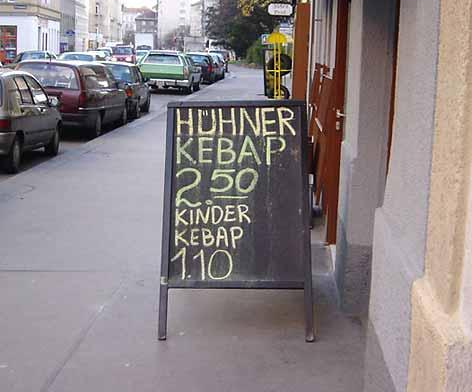
\includegraphics[scale=.55]{material/05Morph-Kebap}
	%\end{figure}
	
\end{frame}


%%%%%%%%%%%%%%%%%%%%%%%%%%%%%%%%%%
%%%%%%%%%%%%%%%%%%%%%%%%%%%%%%%%%%
\subsubsubsection{Rektionskomposita}
%\iftoggle{sectoc}{
%	\frame{
%		\begin{multicols}{2}
%			\frametitle{~}
%			\tableofcontents[currentsection]
%		\end{multicols}
%	}
%}
%%%%%%%%%%%%%%%%%%%%%%%%%%%%%%%%%%

\begin{frame}
\frametitle{Rektionskomposita}

\begin{itemize}
	\item wichtige \textbf{Untergruppe} der Determinativkomposita
	
	\ea Bus\alertred{fahrer} $=$ \gq{\alertred{Fahrer}, der einen Bus fährt}
	\z 
\end{itemize}

\pause 

\begin{block}{Rektion}
	Art der \textbf{syntagmatischen Beziehung} zwischen zwei Einheiten, bei der die eine \textbf{grammatische Eigenschaften} der anderen bestimmt. I.\,d.\,R. redet man von Rektion bei Verben, aber andere Wortarten regieren auch Argumente.  Verben bestimmen bspw.\ den Kasus ihrer Argumente (vgl.\ (\ref{ex:5bKasus2}) \vs (\ref{ex:5bKasus3})) 
	
	\hfill \citep[vgl.][]{McIntyre13a, MyP16e}.

\end{block}

\ea 
	\ea\label{ex:5bKasus2} {Jakob \textbf{unterstützt} [\MyPdown{\alertred{\textsc{akk}}}den Verein].}
	\ex\label{ex:5bKasus3} {Jakob \textbf{hilft} [\MyPdown{\alertred{\textsc{dat}}}dem Verein].}
	\z
\z  

\end{frame}


%%%%%%%%%%%%%%%%%%%%%%%%%%%%%%%%%%
\begin{frame}
\frametitle{Rektionskomposita}

\begin{itemize}
	\item Bedeutungsbeziehung zwischen Erst- und Zweitglied ist durch die \textbf{Argumentstruktur des Zweitglieds} bestimmt (vgl.\ (\ref{ex:5bFolien})), sie ist nicht so ambig wie bei anderen Determinativkomposita (vgl.\ (\ref{ex:5bFischMann})).
	
	\ea 
		\ea\label{ex:5bFischMann} Fisch\alertred{mann} $=$ \gq{Mann, der \textbf{irgendwas} mit Fisch zu tun hat}
		\ex\label{ex:5bFolien} Folien\alertred{bearbeitung} $=$ \gq{Bearbeitung der Folien}
		\z 	
	\z 
\end{itemize}

\begin{itemize}
	\item Häufig findet man Rektionskomposita bei \textbf{deverbalen} Nomina
	

	\ea 
		\ea tag(-en) \ras Tag$+$\alertred{-ung}
		\ex bearbeit(-en) \ras Bearbeit$+$\alertred{-ung}
		\ex fahr(-en) \ras Fahr$+$\alertred{-er}		
		\z 
	\z 
	
\end{itemize}


\end{frame}


%%%%%%%%%%%%%%%%%%%%%%%%%%%%%%%%%%
\begin{frame}
\frametitle{Rektionskomposita}

\begin{itemize}
	
	\item Verb bestimmt, mit wie vielen und mit welchen Argumenten es im Satz erscheint (vgl.\ (\ref{ex:5bBsp1}) \& (\ref{ex:5bBsp2})) (s.\ Rektion, Valenz, Subkategorisierungsrahmen).
	
	\settowidth\jamwidth{[2 ArgumenteX]} 
	\ea \label{ex:5bBsp1} 
		\ea {[\MyPdown{\alertred{\textsc{subj}}}Die \alertred{Linguisten}] \alertblue{tagen}.}
		\jambox{[1 Argument]}
		\ex die \alertblue{Tagung} der Linguisten 
		\ex \alertred{Linguisten}\alertblue{tagung}
		\z 

	\ex \label{ex:5bBsp2} 
		\ea {jemand \alertblue{bearbeitet} [\MyPdown{\alertred{\textsc{obj}}}die \alertred{Folien}].}
		\jambox{[2 Argumente]}
		\ex die \alertblue{Bearbeitung} der Folien
		\ex \alertred{Folien}\alertblue{bearbeitung}
		\z 
	\z
	
	\item \textbf{Erstglied} in einem deverbalen Rektionskompositum realisiert ein \textbf{Argument} des \textbf{Verbs}, das der zweiten Konstituente zugrunde liegt.
	
	\ea	 
		\ea jemand \alertblue{fährt} \alertred{Auto} \ras \alertred{Auto}\alertblue{fahrer}
		\ex jemand \alertblue{beobachtet} das \alertred{Wetter} \ras \alertred{Wetter}\alertblue{beobachter} 
		\ex das \alertred{Rotkehlchen} \alertblue{singt} \ras \alertred{Rotkehlchen}\alertblue{gesang}
		\z 
	\z
		 
\end{itemize}

\end{frame}


%%%%%%%%%%%%%%%%%%%%%%%%%%%%%%%%%%
\begin{frame}
\frametitle{Rektionskomposita}

\begin{itemize}
	\item Es gibt auch Rektionskomposita, bei denen die zweite Konstituente \textbf{nicht deverbal} ist, \zB Nomen oder Adjektiv.
	
	\settowidth\jamwidth{XXXXXXXXXXXXXXXXXXXXXX}
	\ea 
		\ea {[\MyPdown{N}\alertred{Angst} [\MyPdown{PP}vor der \alertblue{Prüfung}]]}
		\jambox{\ras \alertblue{Prüfungs}\alertred{angst}}

		\ex  {[\MyPdown{N}\alertred{Sehnsucht} [\MyPdown{PP}nach dem \alertblue{Tod}]]}
		\jambox{\ras \alertblue{Todes}\alertred{sehnsucht}}
		 
		\ex  {[[\MyPdown{DP}dem \alertblue{Staat}] \MyPdown{A}\alertred{treu}]}
		\jambox{\ras \alertblue{staats}\alertred{treu}}
		
		\ex {[\MyPdown{A}\alertred{sicher} [\MyPdown{PP}vor \alertblue{Fälschung}]]}
		\jambox{\ras \alertblue{fälschungs}\alertred{sicher}}
		
		\ex {[\MyPdown{A}\alertred{frei} [\MyPdown{PP}von \alertblue{Blei}]]}
		\jambox{\ras \alertblue{blei}\alertred{frei}}

		\z 
	\z

		 
\end{itemize}

\end{frame}


%%%%%%%%%%%%%%%%%%%%%%%%%%%%%%%%%%
\begin{frame}
	\frametitle{Übung}
	
	\begin{itemize}
		\item In welchen der folgenden Beispiele liegen Rektionskomposita vor?
		
		\ea\label{ex:05bUE3.1}
			\ea Zigarrenraucher
			\ex Gelegenheitsraucher
			\ex Kettenraucher
			\z
		\ex\label{ex:05bUE3.2}
			\ea Hochschullehrer
			\ex Mathematiklehrer
			\z
		\ex\label{ex:05bUE3.3}
			\ea hitzefrei
			\ex kugelsicher
			\z
		\ex\label{ex:05bUE3.4}
			\ea WDR-Kritiker
			\z
		\z
	\end{itemize}
	
	
\end{frame}

%%%%%%%%%%%%%%%%%%%%%%%%%%%%%%%%%%
\iftoggle{ue-loesung}{
	%%%%%%%%%%%%%%%%%%%%%%%%%%%%%%%%%%
%% UE 3 - 05b Morphologie
%%%%%%%%%%%%%%%%%%%%%%%%%%%%%%%%%%

\begin{frame}
	\frametitle{Übung -- Lösung}
	
\settowidth\jamwidth{zwei Lesarten: Rektionskompositum und kein}
	
\begin{itemize}
	\item In welchen der folgenden Beispiele liegen Rektionskomposita vor?
		
	\begin{exe}
		\exr{ex:05bUE3.1}
		\begin{xlist}
			\ex Zigarrenraucher \loesung{2}{Rektionskompositum}
			\ex Gelegenheitsraucher \loesung{3}{kein Rektionskompositum}
			\ex Kettenraucher \loesung{4}{kein Rektionskompositum}
		\end{xlist}
		\exr{ex:05bUE3.2}
		\begin{xlist}
			\ex Hochschullehrer \loesung{5}{kein Rektionskompositum}
			\ex Mathematiklehrer \loesung{6}{Rektionskompositum}
		\end{xlist}
		\exr{ex:05bUE3.3}
		\begin{xlist}
			\ex hitzefrei \loesung{7}{kein Rektionskompositum}
			\ex kugelsicher \loesung{8}{Rektionskompositum}
		\end{xlist}
		\exr{ex:05bUE3.4}
		\begin{xlist}
			\ex WDR-Kritiker \loesung{9}{zwei Lesarten: Rektionskompositum}
			\loesung{9}{und kein Rektionskompositum}
		\end{xlist}
	\end{exe}

\end{itemize}
	
\end{frame}
}

%%%%%%%%%%%%%%%%%%%%%%%%%%%%%%%%%%


%%%%%%%%%%%%%%%%%%%%%%%%%%%%%%%%%%
%%%%%%%%%%%%%%%%%%%%%%%%%%%%%%%%%%
\subsubsubsection{Possessivkomposita}
%\iftoggle{sectoc}{
%	\frame{
%		\begin{multicols}{2}
%			\frametitle{~}
%			\tableofcontents[currentsection]
%		\end{multicols}
%	}
%}


%%%%%%%%%%%%%%%%%%%%%%%%%%%%%%%%%%
\begin{frame}
\frametitle{Possessivkomposita}

\begin{itemize}
	\item Unterart der \textbf{Determinativkomposita}: Die erste Konstituente bestimmt die zweite näher, das Kompositum bezieht sich aber auf \textbf{eine dritte Entität}, sie sind \textbf{exozentrisch} (\ref{ex:5bexo}) -- im Vgl.\ zu Rektionskomposita und anderen Determinativkomposita, die \textbf{endozentrisch} sind (\ref{ex:5bendo}).
	
	\settowidth\jamwidth{XXXXXXXXXXXXXXXXXXXXXXXXXXXXXXX} 
	\ea\label{ex:5bexo}
		\ea Rot\alertred{kehlchen} \jambox{$=$ \gq{\alertblue{Vogel} mit roter Kehle}, \textbf{kein Kehlchen}}

	
		\ex Rot\alertred{käppchen} \jambox{$=$ \gq{\alertblue{Person} mit roter Kappe}, \textbf{kein Käppchen}}
	
		\ex Lang\alertred{finger} \jambox{$=$ \gq{\alertblue{Person} mit langen Fingern}, \textbf{kein Finger}}
		\z

	
	\ex \label{ex:5bendo}
		\ea Prüfungs\alertred{angst} \jambox{\ras \alertred{Angst}}
		\ex Linguisten\alertred{tagung} \jambox{\ras \alertred{Tagung}}
		\ex Wein\alertred{flasche} \jambox{\ras \alertred{Flasche}}
		\z 
	\z 

\pause 

	\item Der \textbf{morphosyntaktische} Kopf ist die rechte Konstituente (wie immer), aber bzgl.\ der lexikalischen Bedeutung sind Possessivkomposita \textbf{exozentrisch}\\
	\citep[vgl.][]{Fries&MyP16j}.
	
\end{itemize}

\end{frame}


%%%%%%%%%%%%%%%%%%%%%%%%%%%%%%%%%%
%%%%%%%%%%%%%%%%%%%%%%%%%%%%%%%%%%
\subsubsubsection{Kopulativkomposita}
%\iftoggle{sectoc}{
%	\frame{
%		\begin{multicols}{2}
%			\frametitle{~}
%			\tableofcontents[currentsection]
%		\end{multicols}
%	}
%}
%%%%%%%%%%%%%%%%%%%%%%%%%%%%%%%%%%

\begin{frame}
\frametitle{Kopulativkomposita}

\begin{itemize}
	\item keine Unterart der Determinativkomposita: \\
	Erste Konstituente \textbf{bestimmt} die zweite \textbf{nicht näher}.
	
	\ea rot-grün, Fürst-Bischof
	\z 
	
	\item Beide Konstituenten sind \textbf{gleichrangig}.
	
	\item \textbf{Koordinierende} (\dash verknüpfende) Beziehung zwischen den Kompositionsgliedern: Bedeutung des Kompositums ergibt sich \textbf{additiv}.
	
	\settowidth\jamwidth{XXXXXXXXXXXXXXXXXXXXXXXXXXXXXXX} 
	\ea 
		\ea {[süß$+$sauer]} \jambox{$=$ \gq{$x$ ist süß \textbf{und} $x$ ist sauer}}
		\ex {[Spieler$+$Trainer]} \jambox{$=$ \gq{$x$ ist Spieler \textbf{und} $x$ ist Trainer}}
		\z 
	\z 

	\item möglich auch aus mehr als zwei Konstituenten bestehend

	\settowidth\jamwidth{XX[trinäre Struktur]} 		
	\ea rot-rot-grün \jambox{[trinäre Struktur]}
%	\ex süß$+$sauer, nass$+$kalt, rot$+$grün, Fürst-Bischof
%	\ex 
	\z 
	
\end{itemize}

\end{frame}


%%%%%%%%%%%%%%%%%%%%%%%%%%%%%%%%%%
\begin{frame}
\frametitle{Kopulativkomposita}

\begin{itemize}
	\item Konstituenten in Kopulativkomposita haben die \textbf{gleiche Kategorie}.
	
	\ea 
		\ea nass-kalt \ras A $+$ A
		\ex Schauspieler-Regisseur \ras N $+$ N
		\z 
	\z 

\pause 
	
	\item Die Reihenfolge ist im Prinzip \textbf{frei}, aber meistens \textbf{konventionalisiert}.
	
	\ea Strumpfhose \vs ?Hosenstrumpf
	\z 

\pause 
	
	\item Anderes \textbf{Betonungsmuster} als Determinativkomposita: \\
	Bei Determinativkomposita wird der \textbf{Nichtkopf} betont, \\
	bei Kopulativkomposita werden \textbf{alle Konstituenten} betont.
	
	\settowidth\jamwidth{X[Determinativkompositum]} 
	\ea 
		\ea ein \textprimstress blau-\textprimstress grünes \textprimstress Hemd  \jambox{[Kopulativkompositum]}
	
		\ex ein \textprimstress blaugrünes \textprimstress Hemd \jambox{[Determinativkompositum]}
		\z 
	\z

%	\item[] \textbf{ÜB.5}
\end{itemize}


\end{frame}


%%%%%%%%%%%%%%%%%%%%%%%%%%%%%%%%%%
%%%%%%%%%%%%%%%%%%%%%%%%%%%%%%%%%%
\subsubsection{Komposition: Wortstruktur}
%\iftoggle{sectoc}{
%	\frame{
%		\begin{multicols}{2}
%			\frametitle{~}
%			\tableofcontents[currentsection]
%		\end{multicols}
%	}
%}


%%%%%%%%%%%%%%%%%%%%%%%%%%%%%%%%%%
\begin{frame}
\frametitle{Wortstruktur: Kopf}

\begin{itemize}
	\item Bei allen Kompositionsarten gilt das Prinzip der \textbf{Rechtsköpfigkeit}.
	
	\settowidth\jamwidth{X[Determinativkompositum]} 
	\ea 
		\ea die Wein\alertred{flasche} \jambox{[Determinativkompositum]} 
		
			\ea[]{die Weinflasche\alertblue{n} }
			\ex[*]{die Wein\alertblue{e}flasche\alertblue{n}}
			\z 		
		
		\ex die Schnaps\alertred{nase} 	\jambox{\hfill [Possessivkompositum]} 
			\ea[]{die Schnapsnase\alertblue{n} }
			\ex[*]{die Schnäps\alertblue{e}nase\alertblue{n}}
			\z 
	
		
		\ex der Fürst-\alertred{Bischof} \jambox{[Kopulativkompositum]} 
			\ea[]{die Fürst-Bischöf\alertblue{e}}
			\ex[*]{die Fürst\alertblue{en}-Bischöf\alertblue{e}}
			\z 		
		\z 
	\z 

	\item Bspw. bestimmt der Kopf wie das gesamte Kompositum \textbf{flektiert} wird, der Nicht-Kopf wird nicht pluralisiert.

\end{itemize}

\end{frame}


%%%%%%%%%%%%%%%%%%%%%%%%%%%%%%%%%%
\begin{frame}
\frametitle{Wortstruktur: Verzweigung I}

\begin{itemize}
	\item Die meisten Komposita sind \textbf{binär}. \\
	\textbf{Kopulativkomposita} können mehr als zweigliedrig sein.
\begin{figure}
	\centering

\begin{forest}
		[A
			[A [rot]]
			[A [rot]]
			[A [grün]]
		]
\end{forest}	

\end{figure}
%	\item Einige der Kompositionsregeln (aber nicht alle) sind \textbf{rekursiv}.

\end{itemize}
\end{frame}
	
	
%%%%%%%%%%%%%%%%%%%%%%%%%%%%%%%%%%
\begin{frame}
\frametitle{Wortstruktur: Verzweigung II}

%\begin{columns}
%	\begin{column}{.4\textwidth}
%\begin{itemize}
%	\item 
Komposita können
\begin{itemize}
	\item symmetrisch strukturiert (\textbf{beidseitigverzweigend}),
	\item \textbf{linksverzweigend} oder
	\item \textbf{rechtsverzweigend}
\end{itemize}
sein.

\begin{columns}[b]
	
	\begin{column}{.29\textwidth}
	\centering
	\scalebox{.6}{
		\begin{forest}
			[N
				[N
					[A [Groß] ]
					[N [raum] ]
				]
				[N
					[N [flug] ]
					[N [zeug] ]
				]
			]
		\end{forest}
	}
	\end{column}
%%%
	\begin{column}{.32\textwidth}
	\centering
	\scalebox{.6}{
			\begin{forest}
				[N
					[N
						[N
							[N [Berg] ]
							[N [bau] ]
						]
						[N [wissenschaft(-s)] ]
					]
					[N [studium] ]
				]
			\end{forest}
	}	
	\end{column}
%%%
	\begin{column}{.38\textwidth}	
	\centering
	\scalebox{.6}{
		\begin{forest}
			[N
				[N [Bezirk(-s)] ]
				[N
					[N [jahr(-es)] ]
					[N
						[N [haupt] ]
						[N [versammlung] ]
					]
				]
			]
		\end{forest}
	}	
	\end{column}
\end{columns}


%@ee dazu gab es auf jeden Fall eine Übung in den o.g. Aufgaben!
	

\end{frame}


%%%%%%%%%%%%%%%%%%%%%%%%%%%%%%%%%%
\begin{frame}
\frametitle{Wortstrukturregeln: Interpretation}

\begin{itemize}
	\item Komposita können \textbf{strukturell ambig} sein, vgl.\ (\ref{ex:Bsp6}) und (\ref{ex:Bsp7}).
	
	\ea{[[\alertred{Bund(-es)$+$straße(-n)}]$+$\alertblue{bau}] \vs [\alertblue{Bund(-es)}$+$[\alertred{straße(-n)$+$bau}]]}

\pause 
	\ex
	\ea\label{ex:Bsp6}  [[\alertred{Frau(-en)$+$film}]$+$\alertblue{fest}] $=$ \gq{\alertblue{Fest}, das etwas mit \alertred{Frauenfilmen} (\zB Filmen von weiblichen Regisseurinnen) zu tun hat}
	
	\ex\label{ex:Bsp7}  [\alertblue{Frau(-en)}$+$[\alertred{film$+$fest}]] $=$ \gq{\alertred{Filmfest}, das etwas mit \alertblue{Frauen} zu tun hat (\zB Filmfest wird von Frauen organisiert)}
	\z 
	\z 
\end{itemize}

\begin{minipage}{.49\textwidth}

\begin{figure}
\centering
\scalebox{.6}{
\begin{forest}
sm edges,
	[N
		[N
			[N
				[\alertred{Frau(en)}]]
			[N
				[\alertred{film}]]]
		[N
			[\alertblue{fest}]]]
\end{forest}}
\end{figure}

%\ea\label{ex:Bsp6}  ((Frau(-en)$+$film)$+$fest)\\
%$=$ \alertblue{Fest}, das etwas mit \alertred{Frauenfilmen} (\zB Filmen von weiblichen Regisseurinnen) zu tun hat
%\z

\end{minipage}%
%
\hfill ~
%
\begin{minipage}{.49\textwidth}

\begin{figure}
\centering
\scalebox{.6}{
\begin{forest}
sm edges,
	[N
		[N
			[\alertblue{Frau(en)}]]
		[N
			[N
				[\alertred{film}]]
			[N
				[\alertred{fest}]]]]
\end{forest}}
\end{figure}

%\ea\label{ex:Bsp7}  (Frau(-en)$+$(film$+$fest))\\
%$=$ \alertred{Filmfest}, das etwas mit \alertblue{Frauen} zu tun hat (\zB Filmfest wird von Frauen organisiert)
%\z 

\end{minipage}

\pause 

Die \textbf{Betonung} ist je nach Struktur auch unterschiedlich.

\end{frame}


%%%%%%%%%%%%%%%%%%%%%%%%%%%%%%%%%%
\begin{frame}
\frametitle{Wortstrukturregeln: Betonung}

Welche Konstituente trägt die Hauptbetonung in den folgenden Wörtern?

\begin{columns}
\column{.46\textwidth}
	\ea\label{ex:5bFuss} \alertred<2->{Fuß}$+$ball$+$feld
	\ex\label{ex:5bLandes} Landes$+$\alertred<2->{haupt}$+$versammlung
	\z 

\column{.46\textwidth}
	\ea\label{ex:5bWelt} Welt$+$\alertred<2->{nicht}$+$raucher$+$tag
	\ex\label{ex:5bGross} \alertred<2->{Groß}$+$raum$+$flug$+$zeug
	\z 
\end{columns}

\pause 

\begin{itemize}
	\item Betonungs\textbf{tendenzen} bei Det.-Komposita \citep[vgl.][131ff]{Grewendorf&Co91a}:
	\begin{itemize}
		
		\item \textbf{zweigliedrig}: \textbf{Nichtkopf}
	
		\item \textbf{mehrgliedrig}: meist der \textbf{Nichtkopf} \textbf{der verzweigenden Konstituente}
				
		\item \textbf{symmetrisch} verzweigend: \textbf{linke Konstituente} (vgl.\ (\ref{ex:5bGross}))
		
	%	\ea (('Bundes$+$es$+$straße$+$n)$+$bau) \vs (Bund$+$es$+$('straße$+$n$+$bau))
	%	\z
	%	
	%	\ea '((Großraum)$+$(flugzeug))
	%	\z
		
	\end{itemize}
\end{itemize}

\begin{minipage}[t]{.17\textwidth}
	\scalebox{.6}{
		\begin{forest}
			[
			[\alertred{s}
			[\alertred{s} [\alertred{Fuß}]]
			[w [ball]]
			]
			[w [feld]]
			]	
		\end{forest}	
	}
\end{minipage}
%%
\hfill ~
%%
\begin{minipage}[t]{.25\textwidth}
	\scalebox{.6}{
		\begin{forest}
			[
			[w [Landes]]
			[\alertred{s} 
			[\alertred{s} [\alertred{haupt}]]
			[w [versammlung]]
			]
			]	
		\end{forest}	
	}
\end{minipage}
%%
\hfill ~
%%
\begin{minipage}[t]{.21\textwidth}
	\scalebox{.6}{
		\begin{forest}
			[
			[w [Welt]]
			[\alertred{s} 
			[\alertred{s} 
			[\alertred{s} [\alertred{nicht}]]
			[w [raucher]]
			]
			[w [tag]]
			]
			]	
		\end{forest}	
	}
\end{minipage}
%%
\hfill ~
%%
\begin{minipage}[t]{.28\textwidth}
	\scalebox{.6}{
		\begin{forest}
			[
			[\alertred{s} 
			[\alertred{s} [\alertred{Groß}]]
			[w [raum]]
			]
			[w
			[\blue{s} [flug]]
			[w [zeug]]
			]
			]	
		\end{forest}	
	}
\end{minipage}
	
\end{frame}


%%%%%%%%%%%%%%%%%%%%%%%%%%%%%%%%%%%%
%%%%%%%%%%%%%%%%%%%%%%%%%%%%%%%%%%%%
%\subsection{Exkurs: Andere Wortbildungsarten}
%
%\iftoggle{sectoc}{
%	\frame{
%		%		\begin{multicols}{2}
%		\frametitle{~}
%		\tableofcontents[currentsubsection,subsubsectionstyle=hide]
%		%		\end{multicols}
%	}
%}
%
%%%%%%%%%%%%%%%%%%%%%%%%%%%%%%%%%%%
%\begin{frame}
%\frametitle{Exkurs: Andere Wortbildungsarten}
%
%\begin{itemize}
%	\item \textbf{Kontamination} (Wortverschmelzung, -kreuzung, Amalgamierung):
%
%	Verschmelzung zweier Wörter, so dass Wortmaterial aus einem der Originalwörter (oder beider) gelöscht wird.
%		
%	\ea Infotainment, Bioghurt, mainzigartig, Eurasien
%	\z
%	
%	\item \textbf{Generifizierung}: Ausweitung auf Gattungsbezeichnung
%	
%	\ea Tempo (Taschentuch), Fit
%	\z
%	
%	\item \textbf{Analogie}: Bildung eines neuen Wortes durch Ersetzung eines Morphems eines komplexen Wortes durch ein anderes, kontextuell passenderes
%	
%	\ea e-card (von e-mail), slow food (von fast food)
%	\z
%	
%\end{itemize}
%
%\end{frame}
%
%
%%%%%%%%%%%%%%%%%%%%%%%%%%%%%%%%%%%
%\begin{frame}
%\frametitle{Exkurs: Andere Wortbildungsarten}
%
%\begin{itemize}
%\item \textbf{Kurzwortbildung}
%
%\begin{itemize}
%	\item phonetisch ungebunden (\textbf{Abkürzung}):
%	
%	\ea ARD, EU, CIA
%	\z
%	
%	\item phonetisch gebunden (\textbf{Akronym}):
%	
%	\ea DAX, PIN, UFO
%	\z
%
%	\item Weitere Kurzwörter: Wortmaterial am Wortanfang oder -ende wird getilgt.
%	
%	\ea Kripo, Bus, Auto, bi, öko, Schum\alertred{i}, Alk\alertred{i}
%	\z
%	
%\end{itemize}
%
%
%\item \textbf{Wortschöpfung}
%
%\ea Vileda (wie Leder), Iglo, Haribo (Hans Riegel Bonn)
%\z
%
%\end{itemize}
%
%\end{frame}
%
%
%%%%%%%%%%%%%%%%%%%%%%%%%%%%%%%%%%%
%\begin{frame}
%\frametitle{Exkurs: Andere Wortbildungsarten}
%
%\begin{itemize}
%\item \textbf{Rückbildung} (Reanalyse): Umdrehen einer Wortbildungsregel
%
%\begin{itemize}
%\item im Deutschen typisch bei Verben: Ableitung komplexer Verben aus komplexen Substantiven, deren Zweitglied von einem Verb stammt.
%%\item Rückbildung \ras Kürzung?
%\item Verb als Produkt: 
%
%\begin{itemize}
%	\item häufig nur in finaler Satzposition verwendbar
%	
%	\item mit problematischer Verbzweitstellung
%	
%	\item Paradigma manchmal nicht vollständig
%\end{itemize}
%
%\ea bergsteigen, schleichwerben, farbkopieren, mähdreschen
%\z
%
%\item Selten auch bei der Herleitung von Substantiven oder Adjektiven zu finden:
%
%\ea Unsympath
%\z
%
%\end{itemize}
%\end{itemize}
%
%
%\end{frame}
%
%
%%%%%%%%%%%%%%%%%%%%%%%%%%%%%%%%%%%
%\begin{frame}
%\frametitle{Exkurs: Andere Wortbildungsarten}
%
%\begin{itemize}
%\item \textbf{Fremdwortbildung:} Bildung von Wörter nach dem Muster einer Fremdsprache 
%
%	\begin{itemize}
%		\item Diese Wörter gibt es in der Ursprungssprache nicht \\
%		oder nicht mit dieser Bedeutung (vgl. (\ref{ex:M5bFWB1})).
%		
%		\item Produktiv auch mit sog. Konfixen (vgl. (\ref{ex:M5bFWB2}))
%	\end{itemize}
%
%\ea\label{ex:M5bFWB1} Handy, Wellness, Beamer
%
%\ex\label{ex:M5bFWB2} Thermohose, Schokaholic
%\z
%
%
%\item \textbf{Reduplikation}
%
%%\begin{itemize}
%%	\item 
%	
%	\settowidth\jamwidth{XX[komplette Dopplung]} 
%	\ea Blabla, Wauwau \jambox{[komplette Dopplung]}
%	\z
%	
%%	\item :
%	
%	\ea Larifari, Hokuspokus \jambox{[Reimdopplung]}
%	\z
%	
%%	\item :
%	
%	\ea Wirrwarr, Wischiwaschi, Singsang  \jambox{[Ablautdopplung]}
%	\z
%	
%%\end{itemize}
%\end{itemize}
%
%\end{frame}
%
%
%%%%%%%%%%%%%%%%%%%%%%%%%%%%%%%%%%%%
%\begin{frame}
%\frametitle{Exkurs: Andere Wortbildungsarten}
%
%\begin{itemize}
%\item \textbf{Zusammenrückung:}
%
%\begin{itemize}
%\item aus syntaktischen Phrasen hervorgegangen
%\item Wortfolge und Flexionsmarkierungen werden beibehalten
%
%\ea Möchte+gern, in+folge, wasser+triefend
%\z
%
%\end{itemize}
%
%\item \textbf{Zusammenbildung:}
%
%\begin{itemize}
%\item Dreigliedrig: weder die ersten beiden noch die letzten beiden Glieder kommen frei vor.
%\item Sie werden manchmal als Derivation mit einem nicht lexikalischen ersten Teil analysiert.
%
%\ea Schrift+stell+er, Alt+sprach+ler
%\ex 
%	\ea[?]{ {[}V schriftstell-{]} + {[}-er{]} }
%	
%	\vs 
%	
%	\ex[?]{ {[}N Schrift-{]} + {[}N -steller{]}}
%	\z 
%\z
%
%\end{itemize}
%\end{itemize}
%
%
%\end{frame}
%
%
%%%%%%%%%%%%%%%%%%%%%%%%%%%%%%%%%%%
%\begin{frame}
%\frametitle{Exkurs: Andere Wortbildungsarten}
%
%\begin{itemize}
%\item \textbf{Komposition}
%
%\begin{itemize}
%\item Bildung einer komplexen Form, in der zwei (oder mehr) freie Morpheme auftreten
%
%\ea Edelmut, Baukran, Geisteswissenschaft, süßsauer
%\z
%
%\end{itemize}
%
%\end{itemize}
%
%\end{frame}
%
%%%%%%%%%%%%%%%%%%%%%%%%%%%%%%%%%%%
%\begin{frame}
%\frametitle{Exkurs: Andere Wortbildungsarten}
%
%\begin{itemize}
%\item \textbf{Derivation}
%
%\begin{itemize}
%\item Bildung einer komplexen Form, meist mittels Derivationsaffixen, die dem Stamm vorausgehen oder ihm folgen können
%
%\ea Ableit + ung, ver + schlaf-, Un + mensch
%\z
%
%\item Explizite / äußere Derivation: mittels abtrennbarer Affixe
%
%\ea (Grab + ung).
%\z
%
%\item Implizite / innere Derivation: ohne klar abtrennbare Affixe
%
%\ea trink- \vs Trank
%\z
%
%\end{itemize}
%\end{itemize}
%
%\end{frame}
%
%%%%%%%%%%%%%%%%%%%%%%%%%%%%%%%%%%%
%\begin{frame}
%\frametitle{Exkurs: Andere Wortbildungsarten}
%
%\begin{itemize}
%\item \textbf{Konversion:}
%
%\begin{itemize}
%\item Umsetzung eines Stammes in eine andere Kategorie
%\item ohne zusätzliches Morphem oder sonstige Veränderungen
%\item Konversion \ras Derivation? (Derivation mit einem Nullmorphem)
%
%\eal 
%\ex Nomen Dank \vs Verb dank-
%\ex das Blau
%\ex die Betrunkene
%\zl
%
%\end{itemize}
%
%%\item[] \textbf{ÜB.1}
%\end{itemize}
%
%
%\end{frame}
%
%%%%%%%%%%%%%%%%%%%%%%%%%%%%%%%%%%%
%%%%%%%%%%%%%%%%%%%%%%%%%%%%%%%%%%%
\subsection*{Elektronische Quellen}
%%%%%%%%%%%%%%%%%%%%%%%%%%%%%%%%%%%

\begin{frame}[allowframebreaks]{Elektronische Quellen}

\footnotesize

\begin{itemize}
	
	\item LINK -- \gqq{Rindfleischetikettierungsüberwachungsaufgabenübertragungsgesetz}\\
	(Zugriff: 17.04.2019):
	\url{https://de.wikipedia.org/wiki/Rindfleischetikettierungsüberwachungsaufgabenübertragungsgesetz}
	
	\item VIDEO -- \gqq{Spoken Pirahã with subtitles} (Zugriff: 24.10.2013): \url{http://www.youtube.com/watch?v=SHv3-U9VPAs}
	
\end{itemize}

\end{frame}



%%%%%%%%%%%%%%%%%%%%%%%%%%%%%%%%%%%
%%%%%%%%%%%%%%%%%%%%%%%%%%%%%%%%%%%
%\section{X}
%%\frame{
%%\frametitle{~}
%%	\tableofcontents[currentsection]
%%}
%
%
%%%%%%%%%%%%%%%%%%%%%%%%%%%%%%%%%%%
%\begin{frame}
%\frametitle{Y}
%
%\begin{itemize}
%	\item 
%\end{itemize}
%
%
%\end{frame}


%%%%%%%%%%%%%%%%%%%%%%%%%%%%%%%%%%%
%%%%%%%%%%%%%%%%%%%%%%%%%%%%%%%%%%%
%\section{X}
%%\frame{
%%\frametitle{~}
%%	\tableofcontents[currentsection]
%%}
%
%
%%%%%%%%%%%%%%%%%%%%%%%%%%%%%%%%%%%
%\begin{frame}
%\frametitle{Y}
%
%\begin{itemize}
%	\item 
%\end{itemize}
%
%
%\end{frame}
%


%%%%%%%%%%%%%%%%%%%%%%%%%%%%%%%%%%%%%%%%%%%%%%%%
%% Compile the master file!
%% 		Include: Antonio Machicao y Priemer
%% 		Course: GK Linguistik
%%%%%%%%%%%%%%%%%%%%%%%%%%%%%%%%%%%%%%%%%%%%%%%%


%%%%%%%%%%%%%%%%%%%%%%%%%%%%%%%%%%%%%%%%%%%%%%%%%%%%
%%%             Metadata                         
%%%%%%%%%%%%%%%%%%%%%%%%%%%%%%%%%%%%%%%%%%%%%%%%%%%%      

\title{Grundkurs Linguistik}

\subtitle{Morphologie III: Wortbildung II}

\author[A. Machicao y Priemer]{
	{\small Antonio Machicao y Priemer}
	\\
	{\footnotesize \url{http://www.linguistik.hu-berlin.de/staff/amyp}}
	%	\\
	%	{\small\href{mailto:mapriema@hu-berlin.de}{mapriema@hu-berlin.de}}
}

\institute{Institut für deutsche Sprache und Linguistik}

% bitte lassen, sonst kann man nicht sehen, von wann die PDF-Datei ist.
%\date{ }

%\publishers{\textbf{6. linguistischer Methodenworkshop \\ Humboldt-Universität zu Berlin}}

%\hyphenation{nobreak}


%%%%%%%%%%%%%%%%%%%%%%%%%%%%%%%%%%%%%%%%%%%%%%%%%%%%
%%%             Preamble's End                  
%%%%%%%%%%%%%%%%%%%%%%%%%%%%%%%%%%%%%%%%%%%%%%%%%%%%      


%%%%%%%%%%%%%%%%%%%%%%%%%      
\huberlintitlepage[22pt]
\iftoggle{toc}{
	\frame{
		\begin{multicols}{2}
			\frametitle{Inhaltsverzeichnis}\tableofcontents
			%[pausesections]
		\end{multicols}
	}
}


%%%%%%%%%%%%%%%%%%%%%%%%%%%%%%%%%%
%%%%%%%%%%%%%%%%%%%%%%%%%%%%%%%%%%
%%%%%LITERATURE:

%% Allgemein
\nocite{Glueck&Roedel16a}
\nocite{Schierholz&Co18}
\nocite{Luedeling2009a}
\nocite{Meibauer&Co07a} 
\nocite{Repp&Co15a} 

%%% Sprache & Sprachwissenschaft
%\nocite{Fries16c} %Adäquatheit
%\nocite{Fries16a} %Grammatikalität
%\nocite{Fries&MyP16c} %GG
%\nocite{Fries&MyP16b} %Akzeptabilität
%\nocite{Fries&MyP16d} %Kompetenz vs. Performanz

%%% Phonetik & Phonologie
%\nocite{Altmann&Co07a}
%\nocite{DudenAussprache00a}
%\nocite{Hall00a} 
%\nocite{Kohler99a}
%\nocite{Krech&Co09a}
%\nocite{Pompino95a}
%\nocite{Ramers08a}
%\nocite{Ramers&Vater92a}
%\nocite{Rues&Co07a}
%\nocite{WieseR96a}
%\nocite{WieseR11a}

%%% Graphematik
%\nocite{Altmann&Co07a}
%\nocite{Duerscheid04a}
%\nocite{Eisenberg00a}
%\nocite{Fuhrhop08a}
%\nocite{Fuhrhop09a}
%\nocite{Fuhrhop&Co13a}

%% Morphologie
%\nocite{Bauer00a} %Word
\nocite{Eisenberg00a}
\nocite{Fleischer00a} %Wortbildungsprozesse
\nocite{Fleischer&Barz12a} %Einführung Morphologie
\nocite{Fries&MyP16j} %Kopf
%\nocite{Fuhrhop96a} %Fugenelemente
%\nocite{Fuhrhop00a} %Fugenelemente
\nocite{Grewendorf&Co91a} %Betonung bei Komposita
\nocite{Haspelmath2002a}
\nocite{MyP18b} %Kopf
\nocite{Olsen86a} %Morphologie des Deutschen
%\nocite{Olsen14a} %Coordinative Structures
%\nocite{Plungian00a} %Morphologie im Sprachsystem
%\nocite{Salmon00a} %Term Morphology
%\nocite{Wegener03b} %Fugenelemente
%\nocite{Wurzel00a} %Gegenstand Morphologie
%\nocite{Wurzel00b} %Wort


%%%%%%%%%%%%%%%%%%%%%%%%%%%%%%%%%%%
%%%%%%%%%%%%%%%%%%%%%%%%%%%%%%%%%%%
\section{Morphologie III}
%%%%%%%%%%%%%%%%%%%%%%%%%%%%%%%%%%%

\begin{frame}
\frametitle{Begleitlektüre}

%\begin{itemize}
%	\item Derivation und andere Wortbildungsarten:

	\begin{itemize}
		\item \textbf{obligatorisch:}
		\item[] \citet[46--51]{Abramowski2016a}
		\item \textbf{optional:}
		\item[] \citet[Kap. 2, S. 48--66]{Meibauer&Co07a}
		\item[] \citet[Kap.~7]{Luedeling2009a}
		
	\end{itemize}

%\end{itemize}

\end{frame}


%%%%%%%%%%%%%%%%%%%%%%%%%%%%%%%%%%
%%%%%%%%%%%%%%%%%%%%%%%%%%%%%%%%%%
\subsection{Derivation}

\iftoggle{sectoc}{
	\frame{
		%		\begin{multicols}{2}
		\frametitle{~}
		\tableofcontents[currentsubsection,subsubsectionstyle=hide]
		%		\end{multicols}
	}
}

%%%%%%%%%%%%%%%%%%%%%%%%%%%%%%%%%%

\begin{frame}
\frametitle{Derivation}


	\begin{itemize}
		\item Wortbildungsprozess mittels \textbf{Konkatenation}, bei dem ein wortfähiges Element (freies Morphem oder komplexe Basis) mit einem \textbf{Affix} verbunden wird

		\item Derivation und Flexion sind -- formal gesehen -- \textbf{Affigierungen}.
		
		\item Ergebnis der Derivation: \textbf{Derivat}

		\item 	Derivation $\rightarrow$ neue \emph{Wörter} (auch Lexeme oder Lemmata)\\
		Flexion $\rightarrow$ neue Wort\emph{formen}
	
	\end{itemize}
	
\end{frame}


%%%%%%%%%%%%%%%%%%%%%%%%%%%%%%%%%%%
%%%%%%%%%%%%%%%%%%%%%%%%%%%%%%%%%%%

\subsubsection{Die Basis}
%\frame{
%\frametitle{~}
%	\tableofcontents[currentsection]
%}


%%%%%%%%%%%%%%%%%%%%%%%%%%%%%%%%%%%
\begin{frame}
\frametitle{Die Basis}

\begin{itemize}
	\item \textbf{Basis} (Pl. Basen):
	
	\begin{itemize}
		\item etwas, woran etwas affigiert werden kann
		\item Ausgangsform der \textbf{Derivation}
	\end{itemize}
	
	\item Die Basis kann:
	
	\begin{itemize}
		\item \textbf{morphologisch einfach} (eine Wurzel) sein:
		
		\ea trinkbar $\leftarrow$  [trink]$+$[-bar]
		\z
		
		\item oder \textbf{morphologisch komplex} sein:

		\settowidth\jamwidth{[Basis: Wurzel+Affix]X} 		
		
		
		\ea Trinkbarkeit $\leftarrow$  \alertred{[[trink]}$+$\alertred{[-bar]]}$+$[-keit] \jambox{[Basis: Wurzel$+$Affix]}

		\ex trinkwasserartig $\leftarrow$  \alertred{[[trink]}$+$\alertred{[wasser]]}$+$[-artig]  \jambox{[Basis: Kompositum]}
		\z
		
	\end{itemize}
	
\end{itemize}


\end{frame}



%%%%%%%%%%%%%%%%%%%%%%%%%%%%%%%%%%%
\begin{frame}
\frametitle{Basis: Wortartenwechsel}

	\begin{itemize}
		\item Verb \ras Adjektiv, Substantiv
		
		\ea verkauf(-en) \ras \alertred{verkäuf}$+$-lich, \alertred{Verkäuf}$+$-er
		\z
		
		\item Adverb \ras Adjektiv
		
		\ea heute \ras \alertred{heut}$+$-ig
		\z
		
		\item Adjektiv \ras Substantiv, Verb, Adverb
		
		\eal 
			\ex schön \ras \alertred{Schön}$+$-heit, be-$+$\alertred{schön}$+$-igen
			\ex klug \ras \alertred{klug}$+$-erweise
		\zl
		
		\item Substantiv \ras Adjektiv, Verb, Adverb

		\eal 
			\ex Arzt \ras \alertred{ärzt}$+$-lich, ver-$+$\alertred{arzt}(-en)
			\ex Nacht \ras \alertred{nacht}$+$-s
		\zl
		
	\end{itemize}
	
\end{frame}


%%%%%%%%%%%%%%%%%%%%%%%%%%%%%%%%%%%
\begin{frame}
\frametitle{Basis: Wortart}

\begin{itemize}
	\item Wie erkennt man die Wortart der Basis?
	
%	\begin{itemize}
		\item Substantiv oder Verb als Basis der Derivation:
		
		\eal 
			\ex lauf(-en) \ras (der) Lauf
%			\ex Reifen \ras bereifen
			\ex abnehm(-en) \ras Abnahme
		\zl


		\item \textbf{Formeller Hinweis:} Betrachten Sie die \textbf{Affixe}, die für die Derivation benutzt werden. Diese sind nämlich in der Regel bezüglich der Wortart, mit der sie sich verbinden können, \textbf{beschränkt}.
		
\medskip
				
		\item \textbf{Semantischer Hinweis:} Handelt es sich beim Substantiv um ein \textbf{Objekt} (im Sinne von Ding) o.\,ä. ist \emph{meist} das Substantiv zugrunde liegend, handelt es sich aber um einen \textbf{Vorgang}, ist \emph{meist} das Verb zugrunde liegend.
		
%	\end{itemize}
%	
\end{itemize}

\end{frame}


%%%%%%%%%%%%%%%%%%%%%%%%%%%%%%%%%%%
%%%%%%%%%%%%%%%%%%%%%%%%%%%%%%%%%%%
\subsubsection{Suffixe und Präfixe}
%\frame{
%\frametitle{~}           
%	\tableofcontents[currentsection]
%}
%%%%%%%%%%%%%%%%%%%%%%%%%%%%%%%%%%%

\begin{frame}
\frametitle{Suffixe und Präfixe}

\begin{itemize}
	\item \alertred{Suffixe} bestimmen die kategoriale Zugehörigkeit des Derivats.
	
	\item \alertblue{Präfixe} bestimmen \idR die kategoriale Zugehörigkeit des Derivats nicht.
	
	\ea 
	\ea {[}\MyPdown{N}Glück] -- [\MyPdown{\alertred{A}}glück$+$\alertred{-lich}], [\MyPdown{N}\alertblue{Un-}$+$glück]
	%	\z
	
	\ex {[}\MyPdown{V}setz(-en)] -- [\MyPdown{\alertred{N}}Setz$+$\alertred{-ung}], [\MyPdown{V}\alertblue{über-}$+$setz(-en)]
	%	\z
	
	\ex {[}\MyPdown{V}hör(-en)] -- [\MyPdown{\alertred{A}}hör$+$\alertred{-bar}], [\MyPdown{V}\alertblue{ver-}$+$hör(-en)]
	%	\z
	
	\ex {[}\MyPdown{V}acht(-en)] -- [\MyPdown{\alertred{A}}acht$+$\alertred{-bar}], [\MyPdown{V}\alertblue{miss-}$+$acht(-en)]
	\z
	\z 
	
	\medskip 
	
	\item Suffix \ras \textbf{Kopf}
	
	\item Präfix \ras \textbf{kein Kopf}
	
	\item Kopf  \ras \textbf{rechtsperipher} (wie bei der Komposition)
\end{itemize}
\end{frame}


%%%%%%%%%%%%%%%%%%%%%%%%%%%%%%%%%%%%
%\begin{frame}
%\frametitle{Präfix als Kopf?}
%
%\begin{itemize}
%	\item In einigen Fällen \emph{scheinen} Präfixe Verben aus Substantiven, Adjektiven oder Partikeln abzuleiten.
%
%	\settowidth\jamwidth{[Substantivbasis]X} 			
%	\ea be-, ent-, er-, ver-, zer-, durch-, über-, um-, unter- 
%	\z 
%
%		
%		\ea be-$+$sohlen (*sohlen), ent-$+$kernen (*kernen) \jambox{[Substantivbasis]}
%
%		\ex ver-$+$längern (*längern), über-$+$raschen (*raschen) \jambox{[Adjektivbasis]}
%	
%		\ex be-$+$jahen (*jahen), ver-$+$neinen (*neinen) \jambox{[Partikelbasis]}
%		\z
%		
%\end{itemize}
%		
%\pause
%\medskip
%
%\begin{minipage}[c]{0.6\textwidth}	
%	\begin{itemize}
%		\item In solchen Fällen werden \textbf{Präfixe} \emph{manchmal} \textbf{als Köpfe} analysiert.
%		
%		\item Diese Art von Analyse verletzt das \textbf{Rechtsköpfigkeitsprinzip}.
%	\end{itemize}
%\end{minipage}
%%%
%\begin{minipage}[c]{0.35\textwidth}
%	\centering 
%	\small
%	\begin{forest}
%		[V
%		[\alertblue{V}, name=A1
%		[\alertblue{V\MyPup{af}}, name=A0 
%		[be-]
%		]
%		[\alertred{N}, name=
%		[sohle]
%		]
%		]
%		[Fl [-n]]	
%		]
%		{\draw[->,dashed] (A0) to[out=west,in=west] (A1);
%		}
%	\end{forest}
%	
%\end{minipage}
%
%\end{frame}
%
%
%%%%%%%%%%%%%%%%%%%%%%%%%%%%%%%%%%%
\begin{frame}
\frametitle{Präfixe}

\begin{itemize}
	\item Einige Präfixe sind sowohl als \textbf{nominale} als auch als \textbf{adjektivische Präfixe} \textbf{kategorisiert}.
	
	\ea
	\ea erz-: [\alertred{\MyPdown{N\MyPup{af}}Erz-}]$+$feind, [\alertred{\MyPdown{A\MyPup{af}}erz-}]$+$katholisch
	%			\ex[]
	%		\ex ge-: \alertred{Ge-}$+$büsch
	%			\ex[]
	\ex miss-: [\alertred{\MyPdown{N\MyPup{af}}\alertred{Miss-}}]$+$erfolg, [\alertred{\MyPdown{A\MyPup{af}}miss-}]$+$mutig
	%			\ex[]
	\ex un-: [\alertred{\MyPdown{N\MyPup{af}}\alertred{Un-}}]$+$geduld, [\alertred{\MyPdown{A\MyPup{af}}un-}]$+$sauber
	%			\ex[]
	\ex ur-: [\alertred{\MyPdown{N\MyPup{af}}\alertred{Ur-}}]$+$gestein, [\alertred{\MyPdown{A\MyPup{af}}ur-}]$+$alt
	\z 
	\z
\end{itemize}


%%
\begin{minipage}[c]{0.49\textwidth}
	\centering 			
	\begin{forest}
		[N, name=A1
		[\alertred{N\MyPup{af}}, name=V1 
		[Un-]
		]
		[\alertblue{N}, name=A0
		[mensch]
		]
		]
		{\draw[->,dashed] (A0) to[out=east,in=east] (A1);
		}
	\end{forest}
	
\end{minipage}
%%
\begin{minipage}[c]{0.49\textwidth}
	\centering 			
	\begin{forest}
		[A, name=A1
		[\alertred{A\MyPup{af}}, name=V1 
		[un-]
		]
		[\alertblue{A}, name=A0
		[schön]
		]
		]
		{\draw[->,dashed] (A0) to[out=east,in=east] (A1);
		}
	\end{forest}
	
\end{minipage}

\end{frame}


%%%%%%%%%%%%%%%%%%%%%%%%%%%%%%%%%%
%%%%%%%%%%%%%%%%%%%%%%%%%%%%%%%%%%
\subsubsection{Zirkumfixe}
%\frame{
%%\begin{multicols}{2}
%\frametitle{~}
%	\tableofcontents[currentsection, hideallsubsections]
%%\end{multicols}
%}
%%%%%%%%%%%%%%%%%%%%%%%%%%%%%%%%%%
\begin{frame}
\frametitle{Zirkumfixe}

\begin{itemize}
	\item Zirkumfixe sind \textbf{Köpfe}, da sie (\emph{auch}) auf der rechten Seite des Derivats stehen.
	

\settowidth\jamwidth{XXXXXXXXXXXXXXXXXXXXXXXXXXXXXtXXXXX}	
	\ea
	\ea ge- \dots\ -e: \jambox{[\alertred{\MyPdown{N\MyPup{zf}}Ge-}]$+$\alertblue{\MyPdown{V}}lach$+$[\alertred{\MyPdown{N\MyPup{zf}}-e}]}
	
	\ex ge- \dots\ -ig: \jambox{[\alertred{\MyPdown{A\MyPup{zf}}ge-}]$+$\alertblue{\MyPdown{N}}räum$+$[\alertred{\MyPdown{A\MyPup{zf}}-ig}]}
	
	\ex un- \dots\ -lich: \jambox{[\alertred{\MyPdown{A\MyPup{zf}}un-}]$+$\alertblue{\MyPdown{V}}glaub$+$[\alertred{\MyPdown{A\MyPup{zf}}-lich}]}
	
	\ex un- \dots\ -bar: \jambox{[\alertred{\MyPdown{A\MyPup{zf}}un-}]$+$\alertblue{\MyPdown{A}}platt$+$[\alertred{\MyPdown{A\MyPup{zf}}-bar}]}
	%un-kaputt-bar, un-nah-bar
	
	\ex un- \dots\ -sam: 
	\jambox{[\alertred{\MyPdown{A\MyPup{zf}}un-}]$+$\alertblue{\MyPdown{N}}weg$+$[\alertred{\MyPdown{A\MyPup{zf}}-sam}]}
	
	\ex be- \dots\ -t: 
	\jambox{[\alertred{\MyPdown{A\MyPup{zf}}be-}]$+$\alertblue{\MyPdown{N}}jahr$+$[\alertred{\MyPdown{A\MyPup{zf}}-t}]}
	
	\ex ent- \dots\ -t: 
	\jambox{[\alertred{\MyPdown{A\MyPup{zf}}ent-}]$+$\alertblue{\MyPdown{N}}geister$+$[\alertred{\MyPdown{A\MyPup{zf}}-t}]}
	
	\ex zer- \dots\ -t: 
	\jambox{[\alertred{\MyPdown{A\MyPup{zf}}zer-}]$+$\alertblue{\MyPdown{N}}narb$+$[\alertred{\MyPdown{A\MyPup{zf}}-t}]}
	\z 
	\z
\end{itemize}

\end{frame}


%%%%%%%%%%%%%%%%%%%%%%%%%%%%%%%%%%%
\begin{frame}
\frametitle{Zirkumfixe}

\begin{itemize}

\item Zirkumfixe sind \textbf{Köpfe}, da sie (\emph{auch}) auf der rechten Seite des Derivats stehen.

\item Zirkumfixe stellen ein Problem für Strukturierung dar. \ras \textbf{trinäre Struktur}
\end{itemize}

%%
\begin{minipage}[c]{0.49\textwidth}
\centering 			
\begin{forest}
	[N, name=A1
	[\alertred{A\MyPup{zf}}, %name=V1 
	[un-]
	]
	[\alertblue{A}, name=A0
	[kaputt]
	]
	[\alertred{A\MyPup{zf}}, name=V1 
	[-bar]
	]
	]
	{\draw[->,dashed] (V1) to[out=east,in=east] (A1);
	}
\end{forest}

\end{minipage}
%%
\begin{minipage}[c]{0.49\textwidth}
\centering 			
\begin{forest}
	[A, name=A1
	[\alertred{A\MyPup{af}}, name=A2 
	[un-]
	]
	[\alertblue{V}, name=A0
	[glaub]
	]
	[\alertred{A\MyPup{zf}}, name=V1 
	[-lich]
	]
	]
	{\draw[->,dashed] (V1) to[out=east,in=east] (A1);
	}
\end{forest}

\end{minipage}

\ea 
\gll un- glaub -lich $\neq$ [ un- $+$ [\MyPdown{\alertred{A}} glaub {} $+$ -lich ]]\\
{} {} {}  $\neq$ [[\MyPdown{\alertred{V}} un- $+$ {} glaub ] $+$ -lich ]\\
\z 

\end{frame}	

%%%%%%%%%%%%%%%%%%%%%%%%%%%%%%%%%%
%%%%%%%%%%%%%%%%%%%%%%%%%%%%%%%%%%
\subsubsection{Struktur}
%\frame{
%%\begin{multicols}{2}
%\frametitle{~}
%	\tableofcontents[currentsection, hideallsubsections]
%%\end{multicols}
%}
%%%%%%%%%%%%%%%%%%%%%%%%%%%%%%%%%%

\begin{frame}
\frametitle{Struktur}

\begin{minipage}[c]{0.98\textwidth}

\begin{minipage}[c]{0.83\textwidth}

%	\begin{itemize}
%		\item Wortstrukturregel für \textbf{Suffigierung}:

\ea Wortstrukturregel für \textbf{Suffigierung}: \alertred{X} \ras Y \alertred{X}\MyPup{af}
\z 

\begin{itemize}
	\item Das Suffix \emph{-heit} ist ein \textbf{nomenbildendes Suffix}.
	
	\item Das Suffix agiert als \textbf{Kopf}: Es \textbf{projiziert} seine \textbf{morphosyntaktischen Eigenschaften} an den Mutterknoten, \\
	\dash es bestimmt die Eigenschaften des Derivats.
	
\end{itemize}
%	\end{itemize}

\end{minipage}
%%
\begin{minipage}[c]{0.15\textwidth}
\centering 
\begin{forest}
	[\alertred{N}, name=A1
	[\alertblue{A}, name=V1 
	[frei]
	]
	[\alertred{N}\MyPup{af}, name=A0
	[-heit]
	]
	]
	{\draw[->,dashed] (A0) to[out=east,in=east] (A1);
	}
\end{forest}

\end{minipage}

\end{minipage}
%%
\pause

\vspace{.5cm}
%%
\begin{minipage}[c]{0.98\textwidth}

\begin{minipage}[c]{0.83\textwidth}

%	\begin{itemize}

%		\item Wortstrukturregel für \textbf{Präfigierung}:

\ea Wortstrukturregel für \textbf{Präfigierung}: X \ras \alertblue{X}\MyPup{af} \alertblue{X}
\z 

\begin{itemize}
	\item Das Präfix \emph{ver-} ist ein \textbf{Verbaffix}, \dash es verbindet sich\\
	\textbf{nur mit Verben}.
	
	\item Das Präfix agiert \textbf{nicht} als \textbf{Kopf}. Die  \textbf{morphosyntaktischen Eigenschaften} der Basis werden an den Mutterknoten \textbf{projiziert}.
	
\end{itemize}		

%	\end{itemize}

\end{minipage}
%%
%%
\begin{minipage}[c]{0.15\textwidth}
\centering 			
\begin{forest}
	[V, name=A1
	[\alertblue{V}\MyPup{af}, name=V1 
	[ver-]
	]
	[\alertblue{V}, name=A0
	[schreib]
	]
	]
	{\draw[->,dashed] (A0) to[out=east,in=east] (A1);
	}
\end{forest}

\end{minipage}

\end{minipage}

\end{frame}


%%%%%%%%%%%%%%%%%%%%%%%%%%%%%%%%%%

\begin{frame}
\frametitle{Struktur}

\ea Wortstrukturregel für \textbf{Zirkumfigierung}: \alertred{X} \ras \alertred{X}\MyPup{zf} Y \alertred{X}\MyPup{zf}
\z 

\begin{itemize}
\item Das Zirkumfix \emph{Ge- \dots\ -e} ist ein \textbf{nomenbildendes Suffix}.

\item Das Zirkumfix agiert als \textbf{Kopf}: Es \textbf{projiziert} seine \textbf{morphosyntaktischen Eigenschaften} an den Mutterknoten, \\
\dash es bestimmt die Eigenschaften des Derivats.

\end{itemize}

\begin{figure}
\centering 
\begin{forest}
[\alertred{N}, name=A1
[\alertred{N}\MyPup{zf}, name=A2
[Ge-]
]
[\alertblue{V}, name=V1 
[kreisch]
]
[\alertred{N}\MyPup{zf}, name=A0
[-e]
]
]
{\draw[->,dashed] (A0) to[out=east,in=east] (A1);
}
\end{forest}

\end{figure}

\end{frame}


%%%%%%%%%%%%%%%%%%%%%%%%%%%%%%%%%%%
\begin{frame}
\frametitle{Projektion von Eigenschaften}

\begin{itemize}
\item Suffixe und Zirkumfixe (qua Köpfigkeit) bestimmen die \textbf{Kategorie des Derivats}, d.\,h. die Art von Stämmen, die sie bilden.

\ea 
\ea \textbf{substantivbildende} Suffixe: -ung, -heit/-keit, -er, -schaft, \dots

\ex Schreib\alertred{ung}, Frei\alertred{heit}, Rauch\alertred{er}, Hörer\alertred{schaft}
\z 
\z

\ea 
\ea \textbf{adjektivbildende} Suffixe: -bar, -lich, -haft, -ig, \dots 
\ex hör\alertred{bar}, röt\alertred{lich}, lach\alertred{haft}, mut\alertred{ig}
\z 
\z

\ea 
\ea \textbf{verbbildende} Suffixe: -(e)l, -(is/ifiz)ier, -ig, \dots
\ex häk\alertred{el}(n), schläng\alertred{el}(n), stabil\alertred{isier}(en), ängst\alertred{ig}(en)
\z 
\z

\end{itemize}
\end{frame}


%%%%%%%%%%%%%%%%%%%%%%%%%%%%%%%%%%%
\begin{frame}
\frametitle{Projektion von Eigenschaften}

\begin{itemize}

\item Nominale Suffixe und Zirkumfixe bestimmen das \textbf{Genus des Derivats}.

%\vspace{1em}
\begin{multicols}{2}

\begin{exe}
\ex \textbf{-ung}:  Acht $+$ -ung\MyPdown{f}
\ex \textbf{-keit}: Tapfer $+$ -keit\MyPdown{f}
\ex \textbf{-chen}: Häus $+$ -chen\MyPdown{n}
\ex \textbf{-tum}: Brauch $+$ -tum\MyPdown{n}\\
(aber: Reichtum\MyPdown{\alertred{m}})
\end{exe}

\columnbreak

\begin{exe}
\ex \textbf{-ian}: Grob $+$ -ian\MyPdown{m}
\ex \textbf{-ling}: Lehr $+$ -ling\MyPdown{m}
\ex \textbf{-bold}: Witz $+$ -bold\MyPdown{m}
\ex \textbf{ge- -e}: Ge- $+$ heul $+$ -e\MyPdown{n}

~ % wegen Spaltenteilung
\end{exe}

\end{multicols}

\end{itemize}

\end{frame}


%%%%%%%%%%%%%%%%%%%%%%%%%%%%%%%%%%%
\begin{frame}
\frametitle{Rekursivität}

\begin{itemize}
\item Derivation und Komposition sind im Prinzip \textbf{rekursive Wortbildungsprozesse} (d.\,h. sie können mehrfach angewendet werden). 

\item \textbf{Dieselbe Affigierung} kann jedoch in seltenen Fällen erfolgen\\
(vgl.\ (\ref{ex:5bDerRek1}) und (\ref{ex:5bDerRek2})).

\ea 
\ea\label{ex:5bDerRek1} \alertred{Ur-}$+$großmutter, \alertred{Ur-}$+$urgroßmutter, \alertred{Ur-}$+$ururgroßmutter

\ex\label{ex:5bDerRek2} trink$+$\alertred{-bar}, *trinkbar$+$\alertred{-bar}, *trinkbarbar$+$\alertred{-bar}
\z 
\z 

\pause 

\item Einige Affixe (\textbf{Schlussaffixe}) zeigen an, dass \textbf{keine weiteren Suffixe} angeschlossen werden können (vgl.\ \ab{-igkeit} in (\ref{ex:5bEndAff})):

\ea\label{ex:5bEndAff} lehr(-en) \ras Lehr$+$\alertred{-er} \ras lehrer$+$\alertred{-haft} \ras Lehrerhaft$+$\alertred{-igkeit}
\z

\item Rekursion bei der Derivation ist also \textbf{beschränkter} als bei der Komposition.

\end{itemize}


\end{frame}


%%%%%%%%%%%%%%%%%%%%%%%%%%%%%%%%%%
%%%%%%%%%%%%%%%%%%%%%%%%%%%%%%%%%%
\subsubsection{Beschränkungen von Affixen}
%\frame{
%%\begin{multicols}{2}
%\frametitle{~}
%	\tableofcontents[currentsection, hideallsubsections]
%%\end{multicols}
%}
%%%%%%%%%%%%%%%%%%%%%%%%%%%%%%%%%%

\begin{frame}
\frametitle{Beschränkungen von Affixen}

\begin{itemize}
\item Der Kopf bestimmt (bzw. \emph{beschränkt}), \textbf{mit welchen Elementen} er sich verbinden kann.
\item Dabei gibt es verschiedene Arten von Beschränkungen.

\medskip 	

\item \textbf{Syntaktische Beschränkungen}

\begin{itemize}
\item \textit{-bar} verbindet sich mit \textbf{Verben}:

\ea \alertred{les}bar, \alertred{ess}bar, \alertred{erzieh}bar vs. *\alertred{grün}bar
\z

\item \textit{-heit/-keit} verbinden sich mit \textbf{Adjektiven}:		

\ea \alertred{Blöd}heit, \alertred{Frei}heit, \alertred{Unachtsam}keit \vs *\alertred{Les}heit, *\alertred{Ess}keit
\z

\end{itemize}

\item \textbf{Argumentstrukturelle Beschränkungen}

\begin{itemize}
\item \textit{-bar} verbindet sich mit \textbf{transitiven Verben}:	

\ea *\alertred{schlaf}bar, *\alertred{frier}bar
\z

\end{itemize}

\end{itemize}

\end{frame}


%%%%%%%%%%%%%%%%%%%%%%%%%%%%%%%%%%%
\begin{frame}
\frametitle{Beschränkungen von Affixen}

\begin{itemize}
\item \textbf{Phonologische Beschränkungen}

\begin{itemize}
\item \emph{-keit} folgt ausschließlich auf \textbf{unbetonte} Silben: 				

\ea \alertred{\textipa{\textprimstress}Wach}\alertblue{sam}$+$-keit \vs *\alertred{\textipa{\textprimstress}Frei}$+$-keit, *\alertred{\textipa{\textprimstress}Nett}$+$-heit \vs \alertred{\textipa{\textprimstress}Net}\alertblue{tig}$+$-keit
\z

%		\item[]
(aber nicht nach \emph{-haft}, \emph{-los}, \emph{-en}, \emph{-e}: *Schad\alertblue{haft}$+$-keit, *Rast\alertblue{los}$+$-keit, *Mü\alertblue{de}$+$-keit)

\pause 
\medskip 

\item \textit{-heit} lässt \textbf{betonte und unbetonte} Silben zu: 

\ea \alertred{\textipa{\textprimstress}Frei}heit, \alertred{\textipa{\textprimstress}Schüch}\alertblue{tern}heit, 
\z

%		\item[] 
(außer \emph{-e}, \emph{-bar}, \emph{-ig}, \emph{-isch}, \emph{-lich}, \emph{-mäßig}, \emph{-sam}, \emph{-haft}, \emph{-los})

\pause 
\medskip 

\item \emph{-ei} verbindet sich mit Wörtern, deren letzte Silbe \textbf{unbetont} ist (ansonsten werden die Allomorphe \emph{-erei}/\emph{-elei} verwendet): 

\ea Wüs\alertblue{te(n)}$+$-ei \vs \alertred{Renn}$+$-rei, \alertred{Lieb}$+$-elei
\z

\end{itemize}

\end{itemize}

\end{frame}


%%%%%%%%%%%%%%%%%%%%%%%%%%%%%%%%%%%
\begin{frame}
\frametitle{Beschränkungen von Affixen}


\begin{itemize}
\item \textbf{Morphologische Beschränkungen}

\begin{itemize}
\item \emph{Ge-}{\dots}\emph{-e} verbindet sich \textbf{nicht mit komplexen Verben}:

\ea Ge-\alertred{red}-e, Ge-\alertred{mecker}-e \vs *Ge-\alertred{verkauf}-e, *Ge-\alertred{entlass}-e\\
(Aber: \alertblue{Herum}-ge-\alertred{hup}-e)
\z

\pause

\item \emph{-lich} verbindet sich \textbf{nicht mit Abkürzungen}:

\ea \alertred{sport}$+$-lich \vs *\alertred{SPD}$+$-lich, *\alertred{DGfS}$+$-lich
\z

\pause 

\item \emph{-heit} folgt auf \textbf{Partizipien} (\emph{-keit} nicht):

\ea \alertred{Gelassen}$+$-heit, \alertred{Aufgeregt}$+$-heit, \alertred{Zurückgezogen}$+$-heit
\z

\end{itemize}

\end{itemize}

\end{frame}


%%%%%%%%%%%%%%%%%%%%%%%%%%%%%%%%%%%
\begin{frame}
\frametitle{Beschränkungen von Affixen}

\begin{itemize}
\item \textbf{Semantisch-konzeptuelle Beschränkungen}

\begin{itemize}
\item \emph{-fach} verbindet sich nur mit \textbf{Zahlen} und \textbf{Quantitätsausdrücken}:

\ea \alertred{zwei}$+$-fach, \alertred{hundert}$+$-fach, \alertred{viel}$+$-fach, \alertred{mehr}$+$-fach \vs *\alertred{grün}$+$-fach, *\alertred{frei}$+$-fach
\z

\pause

\item \textit{Ge-{\dots}-e} verbindet sich \textbf{nicht mit stativen Verben} (d.\,h. Verben, die einen Zustand ausdrücken):

\ea Ge-\alertred{renn}-e \vs *Ge-\alertred{wiss}-e, *Ge-\alertred{kenn}-e
\z

\end{itemize}

\end{itemize}

\end{frame}


%%%%%%%%%%%%%%%%%%%%%%%%%%%%%%%%%%%
\begin{frame}
\frametitle{Beschränkungen von Affixen}

\begin{itemize}

\item \textbf{Beschränkungen der Herkunft}

\begin{itemize}
\item \emph{-bar} verbindet sich mit \textbf{nativen} und sog. \textbf{neoklassischen} Basen, \emph{-abel} hingegen \textbf{nur mit neoklassischen}: 

\ea 
\ea \alertred{tanz}$+$-bar, \alertred{nachvollzieh}$+$-bar, \alertred{annehm}$+$-bar, \alertred{akzeptier}$+$-bar 
\ex \alertred{akzept}$+$-abel, *\alertred{annehm}$+$-abel (akzeptieren: lat.\ Ursprung)
\z 
\z

\end{itemize}

\pause 

\item \textbf{Fazit:} Beschränkungen können alle linguistischen Ebenen betreffen. 

Diese Information muss im \textbf{Lexikoneintrag} sowohl von \textbf{Basen} als auch von \textbf{Derivationsaffixen} gespeichert sein.	
\end{itemize}

\end{frame}


%%%%%%%%%%%%%%%%%%%%%%%%%%%%%%%%%%
%%%%%%%%%%%%%%%%%%%%%%%%%%%%%%%%%%
\subsubsection{Bedeutung von Affixen}
%\frame{
%%\begin{multicols}{2}
%\frametitle{~}
%	\tableofcontents[currentsection, hideallsubsections]
%%\end{multicols}
%}
%%%%%%%%%%%%%%%%%%%%%%%%%%%%%%%%%%

\begin{frame}
\frametitle{Bedeutung von Affixen}

\begin{itemize}
\item Die Bedeutung der Affixe ist \textbf{nicht immer semantisch eindeutig erfassbar}. Sie sind \textbf{ambig} \size{\citep[vgl.][]{Fries&MyP16k}}.

\item Meist haben Affixe eher eine \textbf{grammatische} als eine lexikalisch-semantische Bedeutung. 

\item Es lassen sich jedoch auch \textbf{produktive} Muster/Reihen mit klarem Funktions/Bedeutungsbeitrag:

\ea 
\ea sich \alertred{ver}fahren, sich \alertred{ver}schreiben, %sich versprechen, sich verlaufen, sich verhören 
\dots\ \ras \gq{$x$ falsch machen}
%	\z

\ex Benzin \alertred{ver}fahren, Tinte \alertred{ver}schreiben, %Geld verspielen
\dots\ \ras \gq{$x$ verbrauchen}\\

\ex Aber:\\
\alertred{ver}kaufen \ras \gq{etw. gegen Geld tauschen}\\
%	verärgern \ras \gq{jemanden ärgerlich machen}\\ % Inchoativ
%	verarmen \ras \gq{arm werden}\\ % Inchoativ
\alertred{ver}hungern \ras \gq{aus Mangel an Nahrung sterben}
\z
\z 
\end{itemize}

\end{frame}


%%%%%%%%%%%%%%%%%%%%%%%%%%%%%%%%%%
\begin{frame}
\frametitle{Bedeutung von Affixen}

\begin{itemize}
\item Viele Suffixe sind \textbf{ambig}. Die Untersuchung ihrer \textbf{Bedeutungsvarianten} ist Untersuchungsgegenstand der Morphologie-Semantik-Schnittstelle.

\ea \emph{-ung:} Ereignis, Zustand oder Objekt \size{\citep[vgl.][]{Doelling15a}}
\ea Die [Absperr\alertred{ung} der Straße]\MyPdown{Ereignis} wurde behindert.
\ex Die [Absperr\alertred{ung} der Straße]\MyPdown{Zustand} wurde aufgehoben.
\ex Die [Absperr\alertred{ung} der Straße]\MyPdown{Objekt} wurde abgebaut.
\z 

\ex \emph{-erei:} iteratives, unerwünschtes Geschehen
\ea Besserwiss\alertred{erei}, Heul\alertred{erei}
\z

\ex \emph{-er}: Agens, Instrument, Geschehen als Einzelakt\\
\hfill \size{\citep[vgl.][]{Alexiadou&Co10c}}
\ea Lehr\alertred{er}, Mal\alertred{er}, Rauch\alertred{er}
\ex Öffn\alertred{er}	
\ex Seufz\alertred{er}, Ausrutsch\alertred{er}, Treff\alertred{er} %(aber: Aufkleber)
\z 
\z 
\end{itemize}

\end{frame}


%%%%%%%%%%%%%%%%%%%%%%%%%%%%%%%%%%%%
%\begin{frame}
%\frametitle{Exkurs: Spezialfälle der Affixbedeutung}
%
%
%Sind die rot markierten Einheiten in den folgenden Wörtern Kompositionsglieder oder Affixe? 
%
%\eal 
%\ex Verkehrs\alertred{-wesen}, Schul\alertred{-wesen}
%
%\ex essens\alertred{-technisch}
%
%%	\ex Laub\alertred{-werk}
%
%\ex \alertred{Haupt-}bahnhof
%
%\ex abgas\alertred{-arm}
%\zl
%
%\pause
%
%\begin{itemize}
%\item Pro \textbf{Kompositionsglied}: Morpheme treten auch \textbf{frei} auf.
%
%\item Pro \textbf{Affix}: viel abstraktere Bedeutung als frei vorkommende Form
%\end{itemize}
%
%\begin{block}{Halbaffixe/Affixoide (Suffixoide, Präfixoide)}
%Wortbildungselemente, die von frei vorkommenden Stämmen \textbf{grammatikalisiert} werden und dabei ihre \textbf{Bedeutung erweitern} bzw. \textbf{abstrakter} machen. Sie sind wie Affixe \textbf{reihenbildend}. In der gebundenen Version sind sie mit der frei vorkommenden Form \textbf{nicht bedeutungsgleich}.
%\end{block}
%
%\end{frame}
%
%
%%%%%%%%%%%%%%%%%%%%%%%%%%%%%%%%%%
%%%%%%%%%%%%%%%%%%%%%%%%%%%%%%%%%%
\subsubsection{Produktive und aktive Muster}
%\frame{
%%\begin{multicols}{2}
%\frametitle{~}
%	\tableofcontents[currentsection, hideallsubsections]
%%\end{multicols}
%}
%%%%%%%%%%%%%%%%%%%%%%%%%%%%%%%%%%

\begin{frame}
\frametitle{Produktive und aktive Muster}

\begin{itemize}
\item Manche Muster sind \textbf{produktiv} andere lediglich \textbf{aktiv}.
\end{itemize}

\begin{block}{produktive Wortbildungsregel}
Eine Wortbildungsregel (oder ein Wortbildungsmuster) ist produktiv, wenn mit ihr \textbf{häufig} \textbf{Neubildungen} vorgenommen werden können. Produktivität ist \textbf{graduell}, \zB sind \emph{-ung} und \emph{-er}-Suffigierungen hochproduktiv (\ref{ex:5cProd1}), während \emph{-eur}-Suffigierungen weniger produktiv sind und weitere Beschränkungen an die Basis stellen (\ref{ex:5cProd2}). 
\hfill \size{(\vgl \citealp{Eins16f}; \citealp[45ff]{Meibauer&Co07a})}
\end{block}

\ea 
\ea \label{ex:5cProd1} Absperr$+$\alertred{-ung}, Les$+$\alertred{-ung}
\ex \label{ex:5cProd2} Fris$+$\alertred{-eur}, Mont$+$\alertred{-eur} %Herkunftsbeschränkung
%	\ex \label{ex:5cProd3}
\z 
\z 

\end{frame}


%%%%%%%%%%%%%%%%%%%%%%%%%%%%%%%%%%
\begin{frame}
\frametitle{Produktive und aktive Muster}

\begin{block}{aktives Wortbildungsmuster}
Ein Wortbildungmuster ist \textbf{aktiv}, wenn \textbf{keine neuen Wörter} nach dem Muster gebildet werden können (oder selten und dann stilistisch markiert), aber das Muster \textbf{erkannt} werden kann (\ref{ex:5cProd4}), d.\,h. das Muster ist \textbf{transparent}.
\end{block}

\ea \label{ex:5cProd4} lieb$+$\alertred{-sam}, unterhalt$+$\alertred{-sam}
\z 

\begin{itemize}
\item Ist ein Muster \textbf{nicht mehr aktiv} und \textbf{nicht mehr transparent}, nimmt man die Form als \textbf{Simplex} wahr.

\ea Ur-$+$sache, Mäd$+$-chen
\z 
\end{itemize}

%\textbf{ÜB.3}	
\end{frame}


%%%%%%%%%%%%%%%%%%%%%%%%%%%%%%%%%%
%%%%%%%%%%%%%%%%%%%%%%%%%%%%%%%%%%
\subsection{Partikelverbbildung}

\iftoggle{sectoc}{
	\frame{
		%		\begin{multicols}{2}
		\frametitle{~}
		\tableofcontents[currentsubsection,subsubsectionstyle=hide]
		%		\end{multicols}
	}
}

%%%%%%%%%%%%%%%%%%%%%%%%%%%%%%%%%%

\begin{frame}
\frametitle{Partikelverbbildung}

\begin{itemize}
\item Komposition oder Derivation?

\ea 
\ea teil$+$nehm(-en)
\ex an$+$mach(-en)
\ex über$+$setz(-en) 
\z 
\z 
\pause 

\item Verben können auch aus \textbf{mehreren Morphemen} zusammengesetzt sein (komplex)

\item \textbf{Derivationssuffigierung} ist in der verbalen Wortbildung eher selten\\
(anders als bei Nomina und Adjektiven)

\begin{itemize}
\item nativ (selten, nicht produktiv): \ab{-el}

\ea läch$+$\alertred{-el}, hüst$+$\alertred{-el}, fremd$+$\alertred{-el}, \dots
\z

\item neoklassisch: \ab{-ier} (Allomorphe: \ab{-ifizier}, \ab{-isier})

\ea prob$+$\alertred{-ier}, elektr$+$\alertred{-ifizier}, alphabet$+$\alertred{-isier}, \dots 
\z
\end{itemize}
\end{itemize}

\end{frame}


%%%%%%%%%%%%%%%%%%%%%%%%%%%%%%%%%%
\begin{frame}
\frametitle{Partikelverbbildung}

\begin{itemize}
\item Die \textbf{produktiven Muster} zur Bildung komplexer Verben verwenden eher \textbf{Präfixe} (\ref{ex:5cPraV}) und \textbf{Partikeln} (\ref{ex:5cPartV}).

\ea 
\ea\label{ex:5cPraV} \alertred{be-}rat(-en), \alertred{ver-}kauf(-en)
\ex\label{ex:5cPartV} \alertred{teil-}nehm(-en), \alertred{fest}mach(-en), \alertred{auf}stell(-en)
\z 
\z 

\item Bei den Präfixverbbildungen handelt es sich um \textbf{Derivation}, da die \textbf{Präfixe} \textbf{gebundene} Affixe sind.


\item Die \textbf{Partikeln} dagegen kommen auch \textbf{frei} vor

\medskip

Partikel $+$ Verb \ras \textbf{Komposition}?

\item In (\ref{ex:5cPartV}): Nomen$+$Verb, Adjektiv$+$Verb, Präposition$+$Verb

\end{itemize}

\end{frame}


%%%%%%%%%%%%%%%%%%%%%%%%%%%%%%%%%%

\begin{frame}{Partikelverbbildung}
Wortbildungsprozess, bei dem -- anders als bei der Derivation -- zwei \textbf{frei vorkommende Formen} (Morpheme oder komplexere Stämme) verbunden werden. Partikelverben sind \textbf{morphologisch} und \textbf{syntaktisch trennbar} -- anders als bei der Komposition \size{\citep[vgl.][]{Eins16g,Eisenberg00a}}. 
\end{frame}



%%%%%%%%%%%%%%%%%%%%%%%%%%%%%%%%%%
%%%%%%%%%%%%%%%%%%%%%%%%%%%%%%%%%%
\subsubsection{Partikelverb \vs Präfixverb}
%\frame{
%	\frametitle{~}
%	%	\begin{multicols}{2}
%	\tableofcontents[currentsection, hideallsubsections]
%	%	\end{multicols}
%}
%%%%%%%%%%%%%%%%%%%%%%%%%%%%%%%%%%

\begin{frame}
\frametitle{Partikelverb \vs Präfixverb}

Partikelverben sind wie folgt von Präfixverben zu unterscheiden:

\ea  
\ea \alertred{an}schreiben 
\ex \alertred{be}schreiben
\z 
\z	
\begin{enumerate}
\item Betonung:

\ea \textipa{\textprimstress}\alertred{an}.schrei.ben \vs be.\textipa{\textprimstress}\alertred{schrei}.ben
\z

\item syntaktische Trennbarkeit:

\eal
\ex Ich \alertred{schreibe} dich \alertred{an}.
\ex Ich \alertred{beschreibe} dich.
\zl

\item morphologische Trennbarkeit:

\eal 
\ex Ich habe dich \alertred{an}ge\alertred{schrieb}en. 
\ex Ich habe dich \alertred{beschrieb}en.
\zl

%	\item \textbf{ÜB.4}	
\end{enumerate}

\end{frame}


%%%%%%%%%%%%%%%%%%%%%%%%%%%%%%%%%%
%%%%%%%%%%%%%%%%%%%%%%%%%%%%%%%%%%
\subsubsection{Simplex-, Präfix- und  Partikelverb}
%\frame{
%	\frametitle{~}
%	%	\begin{multicols}{2}
%	\tableofcontents[currentsection, hideallsubsections]
%	%	\end{multicols}
%}
%%%%%%%%%%%%%%%%%%%%%%%%%%%%%%%%%%

\begin{frame}
\frametitle{Simplex-, Präfix- und  Partikelverb}

\begin{table}
\centering
\scalebox{.93}{
\begin{tabular}{l|p{3cm}|p{3cm}|p{3cm}}
& \textbf{Simplex} & \textbf{Präfixverb} & \textbf{Partikelverb}\\
& \textit{\textbf{kaufen}} & \textit{\textbf{ver $+$ kaufen}} & \textit{\textbf{auf $+$ kaufen}}\\
\hline
\textbf{NS} & [\dots] dass Peter die Firma \alertred{kauft}. & [\dots] dass Peter die Firma \alertred{verkauft}. & [\dots] dass Peter die Firma \alertred{aufkauft}.\\
\hline
\textbf{HS} & Peter \alertred{kauft} die Firma. & Peter \alertred{verkauft} die Firma. & Peter \alertred{kauft} die Firma \alertred{auf}. \\
\hline
\textbf{Inf. mit zu} & Peter denkt nicht daran, die Firma \alertblue{zu}~\alertred{kaufen}. & Peter denkt nicht daran, die Firma \alertblue{zu}~\alertred{verkaufen}. & Peter denkt nicht daran, die Firma \alertred{auf}\alertblue{zu}\alertred{kaufen}.\\
\hline
\textbf{Part. II} & Peter hat die Firma \alertblue{ge}\alertred{kauf}\alertblue{t}. & Peter hat die Firma \alertred{verkauf}\alertblue{t}. & Peter hat die Firma \alertred{auf}\alertblue{ge}\alertred{kauf}\alertblue{t}. \\
\hline
\textbf{Betonung} & \textipa{\textprimstress}\alertred{kauf}.en & ver.\textipa{\textprimstress}\alertred{kauf}.en & \textipa{\textprimstress}\alertred{auf}.kauf.en\\
\end{tabular}
}

\end{table}

\end{frame}



%%%%%%%%%%%%%%%%%%%%%%%%%%%%%%%%%%
%%%%%%%%%%%%%%%%%%%%%%%%%%%%%%%%%%
\subsection{Konversion}

\iftoggle{sectoc}{
	\frame{
		%		\begin{multicols}{2}
		\frametitle{~}
		\tableofcontents[currentsubsection,subsubsectionstyle=hide]
		%		\end{multicols}
	}
}

%%%%%%%%%%%%%%%%%%%%%%%%%%%%%%%%%%

\begin{frame}
\frametitle{Konversion}

\begin{itemize}
\item Konversion ist die \textbf{Umkategorisierung} eines Elements \textbf{ohne} Zuhilfenahme von \textbf{Derivationsaffixen} \size{\citep{Eins16h,Eisenberg00a}}.

\item Konversion ist ein \textbf{nicht-konkatenativer Wortbildungsprozess}.

\eal 
\ex \alertred{\MyPdown{V}}schlaf(-en) \ras (der) \alertred{\MyPdown{N}}Schlaf, (des) Schlaf\alertblue{s}
\ex \alertred{\MyPdown{V}}schlaf(-en) \ras (das) \alertred{\MyPdown{N}}Schlafen, (des) Schlafen\alertblue{s}
%	\ex find(-en) \ras (der) Fund (vgl. gefunden)
\zl

\end{itemize}

\end{frame}


%%%%%%%%%%%%%%%%%%%%%%%%%%%%%%%%%%%
\begin{frame}
\frametitle{verschiedene Möglichkeiten der Umkategorisierung}

%Verschiedene Möglichkeiten der Umkategorisierung:

\medskip 

\begin{minipage}[t][][t]{.47\textwidth}

\textbf{Substantivbildung} aus

\ea \textbf{Adjektiv}\\
\alertred{\MyPdown{A}}blau \ras (das) \alertred{\MyPdown{N}}Blau\\
\alertred{\MyPdown{A}}fremd \ras \alertred{\MyPdown{N}}Fremder, \alertred{\MyPdown{N}}Fremde

\ex \textbf{Verb}\\
\alertred{\MyPdown{V}}schlaf(en) \ras \alertred{\MyPdown{N}}Schlaf \\
\alertred{\MyPdown{V}}les(en) \ras  \alertred{\MyPdown{N}}Lesen

\ex \textbf{Verb/Partizip}\\
\alertred{\MyPdown{V}}angestellt \ras \alertred{\MyPdown{N}}Angestellter\\ 
\alertred{\MyPdown{V}}reisend \ras   \alertred{\MyPdown{N}}Reisender

\ex \textbf{Partikel}\\
\alertred{\MyPdown{Part}}nein \ras  (das)  \alertred{\MyPdown{N}}Nein

%\ex \textbf{syntaktischer Fügung}\\
%ohne Wenn \& Aber\\
%das So-tun-als-ob
\z

\end{minipage}
%%
\pause 
\hfill 
%%
\begin{minipage}[t][][t]{.51\textwidth}
\textbf{Verbbildung} aus 

\ea \textbf{Adjektiv}\\
\alertred{\MyPdown{A}}grün \ras  \alertred{\MyPdown{V}}grün(en)\\ 
\alertred{\MyPdown{A}}rot \ras  \alertred{\MyPdown{V}}röt(en)

\ex \textbf{Substantiv}\\
\alertred{\MyPdown{N}}Öl \ras  \alertred{\MyPdown{V}}öl(en)
\z

\pause 
\medskip 

\textbf{Adjektivbildung} aus

\ea \textbf{Substantiv}\\
(der) \alertred{\MyPdown{N}}Ernst \ras  \alertred{\MyPdown{N}}ernst(e)

\ex \textbf{Verb/Partizip}\\
\alertred{\MyPdown{V}}reizend \ras  \alertred{\MyPdown{A}}reizend(e) \\
\alertred{\MyPdown{V}}ausgezeichnet~\ra~\alertred{\MyPdown{A}}ausgezeichnet(e)
\z

%\item \textbf{ÜB.4}

\end{minipage}

\end{frame}


%%%%%%%%%%%%%%%%%%%%%%%%%%%%%%%%%%
%%%%%%%%%%%%%%%%%%%%%%%%%%%%%%%%%%
\subsubsection{Untertypen der Konversion}
%\frame{
%	\frametitle{~}
%	%	\begin{multicols}{2}
%	\tableofcontents[currentsection, hideallsubsections]
%	%	\end{multicols}
%}
%%%%%%%%%%%%%%%%%%%%%%%%%%%%%%%%%%

\begin{frame}
\frametitle{Untertypen der Konversion}


\begin{block}{Morphologische Konversion}
Umkategorisierung eines \textbf{Stammes ohne Flexionselemente}
\end{block}

\eal 
\ex \alertred{\MyPdown{V}}\alertblue{lauf}(-en) \ras (der) \alertred{\MyPdown{N}}\alertblue{Lauf}
\ex \alertred{\MyPdown{N}}\alertblue{Kleid} \ras \alertred{\MyPdown{V}}\alertblue{kleid}(-en)
\zl

\pause 

\begin{block}{Syntaktische Konversion}
Umkategorisierung eines \textbf{Stammes mit Flexionselementen}. In einigen Ansätzen wird die syntaktische Konversion als \textbf{syntaktisches} (und nicht als morphologisches) \textbf{Phänomen} analysiert.
\end{block}

\eal 
\ex \alertred{\MyPdown{V}}lauf(\alertred{-en}) \ras  (das) \alertred{\MyPdown{V}}Lauf\alertblue{en} 
\ex \alertred{\MyPdown{A}}arbeitslos(\alertred{-e})/(\alertred{-er}) \ras (der) \alertred{\MyPdown{N}}Arbeitslos\alertblue{e}, (ein) \alertred{\MyPdown{N}}Arbeitslos\alertblue{er}
%	\ex gefallen(-e) \ras der/die/das Gefallene, ein Gefallener
\zl

\end{frame}


%%%%%%%%%%%%%%%%%%%%%%%%%%%%%%%%%%
\begin{frame}
\frametitle{Konversion \vs implizite Derivation}

\begin{itemize}
\item Bei der Konversion werden \textbf{keine Affixe} für die Umkategorisierung verwendet.

\item Bei der \textbf{impliziten Derivation} (\ref{ex:5cImplDer}) handelt es ich um die Umkategorisierung eines Stammes mittels \textbf{Ablaut} (\zB\ \textipa{[I]} \ras \textipa{[U]}), aber ohne Affixe (wie in der \textbf{expliziten Derivation} (\ref{ex:5cExplDer})).

\ea \label{ex:5cImplDer}
\ea \alertred{\MyPdown{V}}find(-en) \ras \alertred{\MyPdown{N}}F\alertblue{u}nd
\ex \alertred{\MyPdown{V}}greif(-en) \ras \alertred{\MyPdown{N}}Gr\alertblue{i}ff
\z 
\ex \label{ex:5cExplDer} \alertred{\MyPdown{V}}trink(-en) \ras \alertred{\MyPdown{A}}trink$+$bar	
\z 

\item Die Behandlung von impliziten Derivationen als Konversionen ist jedoch \textbf{umstritten} (aufgrund der \emph{Veränderung} im Stamm). Bei der \textbf{Konversion im strengeren Sinne} soll es \textbf{keinerlei Veränderung} geben.

\item Die \textbf{implizite Derivation} ist im Deutschen \textbf{nicht mehr produktiv}.
\end{itemize}

\end{frame}


%%%%%%%%%%%%%%%%%%%%%%%%%%%%%%%%%%
%%%%%%%%%%%%%%%%%%%%%%%%%%%%%%%%%%
\subsubsection{Struktur der Konversion}
%\frame{
%	\frametitle{~}
%	%	\begin{multicols}{2}
%	\tableofcontents[currentsection, hideallsubsections]
%	%	\end{multicols}
%}
%%%%%%%%%%%%%%%%%%%%%%%%%%%%%%%%%%

\begin{frame}
\frametitle{Struktur der Konversion}

\begin{itemize}
\item Konversionen werden als \textbf{unäre Projektionen} analysiert (vgl.\ Abb. \ref{fig:5cKonUnary}). 

\item Unäre Projektionen sind für das \textbf{Köpfigkeitsprinzip} problematisch.

Beachten Sie, dass das \textbf{Flexionssuffix kein morphologischer Kopf} ist!

\end{itemize}

\begin{minipage}{.49\textwidth}

\begin{figure}	
\centering
\scalebox{.7}{
\begin{forest}
sn edges,
[V
[\alertred{V}, name=Verb
[\alertred{N}, name=Noun
[gras]
]
]
[Fl [-en]]
]{
\draw[->,dashed] (Noun) to[out=west,in=west] (Verb);
}
\end{forest}}
\caption{unäre Struktur}
\label{fig:5cKonUnary}
\end{figure}

\end{minipage}
%
\hfill %
\pause %
%
\begin{minipage}{.49\textwidth}

\begin{figure}	
\centering
\scalebox{.7}{
\begin{forest}
sn edges,
[V
[\alertred{V}, name=Verb
[N, name=Noun
[gras]
]
[\alertred{V\MyPup{af}}, name=VerbAf
[$\emptyset$]
]
]
[Fl [-en]]
]{
\draw[->,dashed] (VerbAf) to[out=east,in=east] (Verb);
}
\end{forest}}
\caption{Konversion als Derivation}
\label{fig:5cKonDer}
\end{figure}

\end{minipage}	

\begin{itemize}
\item<2-> \textbf{Alternativ} wird \textbf{Konversion} \textbf{als explizite Ableitung} analysiert (s. rechts), bei der ein \textbf{Nullmorphem}, d.\,h. ein phonetisch leeres Element ($\emptyset$), als Kopf der Derivation angenommen wird (aus anderen Gründen problematisch). 

\item<2-> \textbf{In diesem Kurs} behandeln wir Konversionen als \textbf{unäre Projektionen}.
\end{itemize}

\end{frame}


%%%%%%%%%%%%%%%%%%%%%%%%%%%%%%%%%%%
%%%%%%%%%%%%%%%%%%%%%%%%%%%%%%%%%%%
%\subsection{Exkurs: Andere Wortbildungsarten}
%
%\iftoggle{sectoc}{
%	\frame{
%		%		\begin{multicols}{2}
%		\frametitle{~}
%		\tableofcontents[currentsubsection,subsubsectionstyle=hide]
%		%		\end{multicols}
%	}
%}
%
%%%%%%%%%%%%%%%%%%%%%%%%%%%%%%%%%%%
%
%\begin{frame}
%\frametitle{Exkurs: Andere Wortbildungsarten}
%
%
%\textbf{Rückbildung} (Reanalyse): häufig zur Bildung von Verben verwendete Umdrehung einer Wortbildungsregel
%
%\ea staubsaugen:\\
%\alertred{\MyPdown{V}}saug- \ras \alertred{\MyPdown{N}}Saug $+$ -er \ras \alertred{\MyPdown{N}}Staub $+$ sauger \ras \alertred{\MyPdown{V}}staubsaug(-en)
%\z
%
%\begin{itemize}
%
%\item Verb als Ergebnis der Regel tritt häufig nur in \textbf{finaler Satzposition} (keine V2-Stellung), und hat \idR \textbf{kein vollständiges Paradigma}.
%
%
%\ea 
%\ea[]{bergsteigen, schleichwerben, farbkopieren, bausparen, notlanden}
%%				mähdreschen
%\ex[]{Sie mussten wieder \alertred{schleichwerben}.}
%\ex[]{Sie haben lange \alertred{baugespart}.}
%\ex[*]{Sie \alertred{werben} wieder \alertred{schleich}.}
%\z 
%\z
%
%\item seltener auch bei der Bildung von Nomina oder Adjektiven
%
%\ea sympath \ras sympath $+$ -isch \ras un- $+$ sympathisch \ras Unsympath
%\z
%
%\end{itemize}
%
%%\end{itemize}
%
%\end{frame}
%
%
%%%%%%%%%%%%%%%%%%%%%%%%%%%%%%%%%%%%
%\begin{frame}
%\frametitle{Exkurs: Andere Wortbildungsarten}
%
%\textbf{Phrasenkomposition} (auch Zusammenrückung): recht produktive Zusammenrückung \textbf{syntaktischer Phrasen}, wobei Wortfolge und Flexionsmarkierungen beibehalten werden. Einige sind bereits lexikalisiert (\ref{ex:5SonstWBA}).
%
%\settowidth\jamwidth{[Bsp. in (XX) aus Pafel 2017I]} 	
%\ea \label{ex:5SonstWBA} Möchte$+$gern, in$+$folge, wasser$+$triefend
%
%\ex \label{ex:5PKomp0}
%\ea (das) Das-haben-wir-immer-schon-so-gemacht
%
%%		\ex Kaufe-Ihr-Auto-Kärtchen
%\ex Zwischen-den-Zeilen \gq{Ihr könnt mich mal}-Attitüde
%\ex \gq{Ich werde-dich-ewig-lieben}-Briefchen
%\ex Lauf-dich-gesund-Bewegung 		
%\jambox{[Bsp. in (\ref{ex:5PKomp0}) aus \size{\citealp{Pafel17a}}]}
%\z
%\z
%
%
%%\medskip
%\pause 
%
%
%\textbf{Zusammenbildung:} Dreigliedrige Konkatenation von Elementen. \textbf{Weder die ersten} beiden \textbf{noch die letzten} beiden Glieder kommen \textbf{frei} vor. Sie werden manchmal als \textbf{Derivation} mit einem \textbf{nicht lexikalischen ersten Teil} analysiert.
%
%\ea Schrift$+$stell$+$er, Alt$+$sprach$+$ler
%\ex 
%\ea[?]{ {[}\MyPdown{V} schriftstell-{]} $+$ {[}\MyPdown{N\MyPup{af}} -er{]} }
%\ex[?]{ {[}\MyPdown{N} Schrift{]} $+$ {[}\MyPdown{N} steller{]}}
%\z 
%\z
%
%%\item[] \textbf{ÜB.1}
%
%\end{frame}
%
%
%%%%%%%%%%%%%%%%%%%%%%%%%%%%%%%%%%%
%\begin{frame}
%
%
%\textbf{Kontamination} (Wortverschmelzung, -kreuzung, Amalgamierung):
%
%Verschmelzung zweier Wörter, so dass Wortmaterial aus einem der Originalwörter (oder aus beiden) getilgt wird.
%
%\ea 
%\ea Info\alertred{rmation} $+$ \alertred{Enter}tainment \ras Info$+$tainment
%\ex Bio\alertred{logisch} $+$ \alertred{Jo}ghurt \ras Bio$+$ghurt 
%\ex Mainz $+$ \alertred{einz}igartig \ras mainz$+$igartig
%\ex Eur\alertred{opa} $+$ Asien \ras Eur$+$asien
%\z 
%\z
%
%
%\medskip
%\pause 
%
%
%\textbf{Kurzwortbildung}:
%
%\settowidth\jamwidth{I[phonetisch ungebunden: \textbf{Abkürzung}]} 
%\ea ARD, EU, CIA
%\jambox{[phonetisch ungebunden: \textbf{Abkürzung}]} 
%\z
%
%\ea DAX, PIN, UFO
%\jambox{[phonetisch gebunden: \textbf{Akronym}]} 
%\z
%
%
%\medskip
%
%
%\textbf{Sonstige Kurzwörter:} Wortmaterial am Wortanfang oder -ende wird getilgt.
%
%\ea Kripo, Bus, Auto, bi, öko, Schum\alertred{i}, Alk\alertred{i}, Schok\alertred{i}
%\z
%
%\end{frame}
%
%
%%%%%%%%%%%%%%%%%%%%%%%%%%%%%%%%%%%
%\begin{frame}
%
%
%
%\textbf{Analogie:} Bildung eines neuen Wortes durch Ersetzung eines Morphems eines komplexen Wortes durch ein anderes
%
%\ea e-\alertred{card} (von \emph{e-mail}), \alertred{slow} food (von \emph{fast food})
%\z
%
%
%\medskip
%\pause 
%
%
%\textbf{Reduplikation:}
%
%\settowidth\jamwidth{XX[komplette Dopplung]} 
%\ea Bla$+$bla, Wau$+$wau \jambox{[komplette Dopplung]}
%
%\ex L\alertred{ari}$+$f\alertred{ari}, H\alertred{okus}$+$p\alertred{okus} \jambox{[Reimdopplung]}
%
%\ex W\alertred{i}rr$+$w\alertred{a}rr, W\alertred{i}schi$+$w\alertred{a}schi, S\alertred{i}ng$+$s\alertred{a}ng  \jambox{[Ablautdopplung]}
%\z
%
%\end{frame}
%
%
%%%%%%%%%%%%%%%%%%%%%%%%%%%%%%%%%%%
%\begin{frame}
%
%
%\textbf{Generifizierung:} Ausweitung auf Gattungsbezeichnung
%
%\ea Tempo (für \gq{Taschentücher}), Edding (für \gq{Permanentmarker}),\\Zewa (für \gq{Küchenpapier}), TippEx (für \gq{Korrekturflüssigkeit})
%\z
%
%
%\medskip
%\pause 
%
%
%\textbf{Wortschöpfung:}
%
%\ea Vileda (\emph{wie Leder}), Iglo (von \emph{Iglu}), Haribo (\emph{Hans Riegel Bonn})
%\z
%
%
%\medskip
%\pause 
%
%
%\textbf{Fremdwortbildung:} Bildung von Wörter nach dem Muster einer Fremdsprache. Diese Wörter gibt es in der \textbf{Ursprungssprache} nicht oder nicht mit dieser Bedeutung (vgl. (\ref{ex:M5bFWB1})). Prozess ist auch produktiv auch mit sog. \textbf{Konfixen} (vgl. (\ref{ex:M5bFWB2}))
%
%\ea\label{ex:M5bFWB1} Handy, Wellness, Beamer
%
%\ex\label{ex:M5bFWB2} \alertred{Thermo}$+$hose, Schok$+$\alertred{-aholic}
%\z
%
%\end{frame}
%
%
%%%%%%%%%%%%%%%%%%%%%%%%%%%%%%%%%%%
%%%%%%%%%%%%%%%%%%%%%%%%%%%%%%%%%%%
%todo @ee HA komplett nach 05d verschieben
\subsection{Hausaufgabe}
%
%\iftoggle{sectoc}{
%	\frame{
%		%		\begin{multicols}{2}
%		\frametitle{~}
%		\tableofcontents[currentsubsection,subsubsectionstyle=hide]
%		%		\end{multicols}
%	}
%}
%
%%%%%%%%%%%%%%%%%%%%%%%%%%%%%%%%%%%

%% @ee	Muss irgendiwe aufgeteilt werden auf 05c und 05d
%%			Aufg. 9 muss auf jeden Fall nach 05d

\begin{frame}
\frametitle{Hausaufgabe}


\begin{enumerate}
	\item Kreuzen Sie die korrekten Aussagen an: %\hfill(0,5 Punkte pro Aussage)\\
	
	\begin{itemize}
		\item[$\circ$] Die Graphemkette \emph{abarbeiten} ist ein einzelnes phonologisches Wort im Deutschen.
		\item[$\circ$] \emph{Morphologieeinführungsbuch} ist ein orthographisch-graphemisches Wort des Deutschen, sowie \emph{introductory morphology book} ein orthographisch-graphemisches Wort des Englischen ist.
		\item[$\circ$] Ein Morphem ist die kleinste bedeutungsunterscheidende Einheit in einem bestimmten Sprachsystem.
		\item[$\circ$] \ab{Brot} und \ab{Bröt} sind Allomorphe eines einzelnen Morphems.
	\end{itemize}
	
	\item Erklären Sie das Prinzip der Rechtsköpfigkeit in der Morphologie des Deutschen. Verwenden Sie bei Ihrer Erklärung die unten angegebenen Beispiele. %\hfill(4 Punkte)\\
	
	\eal\label{ex:05cHA2}
	\ex\label{ex:05cHA2a} lichtblau, Blaulicht
	\ex\label{ex:05cHA2b} die Fotowelt, das Weltfoto
	\ex\label{ex:05cHA2c} der Bücherrücken/die Bücherrücken, das Rückenbuch/die Rückenbücher
	\zl
\end{enumerate}

\end{frame}


%%%%%%%%%%%%%%%%%%%%%%%%%%%%%%%%%%%
\begin{frame}
\frametitle{Hausaufgabe}

\begin{itemize}
\item[3.] Geben Sie Argumente für oder gegen die Behandlung von \emph{ver-} in den folgenden Wörtern als Morphem an. Wenn es sich um ein Morphem handelt, ist das immer das gleiche Morphem? %(4 Punkte)

\eal\label{ex:05cHA3}
\ex\label{ex:05cHA3a} \emph{Ver}zweiflung
\ex\label{ex:05cHA3b} \emph{Ver}s
\ex\label{ex:05cHA3c} \emph{ver}kaufen
\ex\label{ex:05cHA3d} \emph{ver}schreiben
\ex\label{ex:05cHA3e} \emph{ver}fahren
\zl

\end{itemize}
\end{frame}


%%%%%%%%%%%%%%%%%%%%%%%%%%%%%%%%%%%
\begin{frame}
\frametitle{Hausaufgabe}

\begin{itemize}
\item[4.] Ordnen Sie die Wortbildungsprozesse links den passenden Beispielen rechts zu (dazu müssen Sie nur den entsprechenden Buchstaben neben das passende Beispiel schreiben). %(0,5 Punkte pro Aussage)
%\end{itemize}

\begin{table}[h!]
\begin{minipage}{0.4\linewidth}
\centering
\begin{tabular}{l|p{0.1\textwidth}|}
	Determinativkompositum & (A)\\
	\hline
	Konversion & (B)\\
	\hline
	Zirkumfigierung (Derivation) & (C)\\
	\hline
	Rektionskompositum & (D)\\
	\hline
	Possessivkompositum & (E)\\
\end{tabular}

\end{minipage}\hfill%
\begin{minipage}{0.4\linewidth}
\centering
\begin{tabular}{|p{0.1\textwidth}|r}
	& \emph{Gerede} \\
	\hline
	& \emph{Milchgesicht}\\
	\hline
	& \emph{Lauf} \\
	\hline
	& \emph{Kettenraucher}  \\
	\hline
	& \emph{Klausurbesprechung}  \\
\end{tabular}
\end{minipage}
\end{table}

		
\item [5.] Geben Sie für die folgende Wortform die Flexionskategorien an, nach denen sie flektiert ist.\\
%\hfill(3 Punkte)\\
\ea\label{ex:05cHA5}
bestehe
\z

\end{itemize}

\end{frame}


%%%%%%%%%%%%%%%%%%%%%%%%%%%%%%%%%%%
\begin{frame}
\frametitle{Hausaufgabe}

\begin{itemize}
\item[6.] Warum sind die Wörter unter (\ref{ex:05cHA6a}) grammatisch und die unter (\ref{ex:05cHA6b}) ungrammatisch? %(4 Punkte)
\eal\label{ex:05cHA6}
\ex\label{ex:05cHA6a} kaufbar, trinkbar
\ex\label{ex:05cHA6b} *fensterbar, *helfbar, *schönbar
\zl

\item [7.] Sind die folgenden Verben Präfixverben oder Partikelverben? Begründen Sie Ihre Entscheidungen. %(3 Punkte)

\eal\label{ex:05cHA7}
\ex auskennen
\ex erkennen
\ex aberkennen
\zl

\item [8.] Geben Sie für das folgende Wort eine morphologische Konstituentenstruktur (inklusive Konstituentenkategorien (N, N\textsuperscript{af}, V, V\textsuperscript{af}, \dots)) an, und bestimmen Sie für jeden Knoten den Wortbildungstyp. %(6,5 Punkte)

\ea\label{ex:05cHA8}
Wahlkampfberaterinnen
\z

\end{itemize}

\end{frame}


%%%%%%%%%%%%%%%%%%%%%%%%%%%%%%%%%%%
\begin{frame}
\frametitle{Hausaufgabe}

\begin{itemize}

\item [9.] Paraphrasieren Sie das folgende komplexe Wort so, dass es der angegebenen Struktur entspricht (auch wenn Sie selbst eine andere Struktur plausibler finden sollten). %(2 Punkte)

\begin{forest}sn edges,
[N
[N[N[Reserve]]
[N[V[lehr]][N\textsuperscript{af}[-er]]]]
[N[zimmer]]
]
\end{forest}

\end{itemize}

\end{frame}


%%%%%%%%%%%%%%%%%%%%%%%%%%%%%%%%%
%%%%%%%%%%%%%%%%%%%%%%%%%%%%%%%%%
\iftoggle{ha-loesung}{
	%%%%%%%%%%%%%%%%%%%%%%%%%%%%%%%%%%
%% HA 1 - 05c Morphologie
%%%%%%%%%%%%%%%%%%%%%%%%%%%%%%%%%%

\begin{frame}{Hausaufgabe -- Lösung}

\begin{enumerate}
	\item Kreuzen Sie die korrekten Aussagen an %\hfill(0,5 Punkte pro Aussage)\\

\begin{itemize}
	\item[$\circ$] Die Graphemkette abarbeiten ist ein einzelnes phonologisches Wort im Deutschen.
	\item[$\circ$] \emph{Morphologieeinführungsbuch} ist ein orthographisch-graphemisches Wort des Deutschen, sowie \emph{introductory morphology book} ein orthographisch-graphemisches Wort des Englischen ist.
	\item[$\circ$] Ein Morphem ist die kleinste bedeutungsunterscheidende Einheit in einem bestimmten Sprachsystem.
	\alertgreen{
			\item[\alertgreen{$\checkmark$}] \ab{Brot} und \ab{Bröt} sind Allomorphe eines einzelnen Morphems.
		}
\end{itemize}

\end{enumerate}
\end{frame}


%%%%%%%%%%%%%%%%%%%%%%%%%%%%%%%%%%
\begin{frame}{Hausaufgabe -- Lösung}

\begin{enumerate}
	\item[2.] Erklären Sie das Prinzip der Rechtsköpfigkeit in der Morphologie des Deutschen. Verwenden Sie bei Ihrer Erklärung die unten angegebenen Beispiele. %\hfill(4 Punkte)\\

\begin{exe}
	\exr{ex:05cHA2}
	\begin{xlist}
		\ex lichtblau, Blaulicht
		\ex die Fotowelt, das Weltfoto
		\ex	die Bücherrücken, die Rückenbücher
	\end{xlist}
\end{exe}

\pause

\alertgreen{Der Kopf eines Wortes ist immer rechtsperipher. Er bestimmt die morphosyntaktischen Eigenschaften eines Wortes sowie viele semantische Aspekte, \zB}

	\begin{itemize}
		\item[\alertgreen{--}] \alertgreen{(\ref{ex:05cHA2a}): Wortart (A \vs N)}
		\item[\alertgreen{--}] \alertgreen{(\ref{ex:05cHA2b}): Genus (f \vs n)}
		\item[\alertgreen{--}] \alertgreen{(\ref{ex:05cHA2c}): Pluralflexion (endungslos \vs \emph{-er})}
		\item[\alertgreen{--}] \alertgreen{Bei Determinativkomposita bildet das Kompositum eine Unterart des Kopfes, bspw. geht es in (\ref{ex:05cHA2c}) im ersten Fall um einen bestimmen Blauton und im zweiten um eine bestimmte Art von Licht.}
	\end{itemize}

\end{enumerate}
\end{frame}


%%%%%%%%%%%%%%%%%%%%%%%%%%%%%%%%%

\begin{frame}{Hausaufgabe -- Lösung}

\begin{enumerate}
\item[3.] Geben Sie Argumente für oder gegen die Behandlung von \emph{ver-} in den folgenden Wörtern als Morphem an. Wenn es sich um ein Morphem handelt, ist das immer das gleiche Morphem?%\\
%\hfill(4 Punkte)\\

\begin{exe}
	\exr{ex:05cHA3}
	\begin{xlist}
		\ex \emph{Ver}zweiflung
		\ex \emph{Ver}s
		\ex \emph{ver}kaufen
		\ex \emph{ver}schreiben
		\ex \emph{ver}fahren
	\end{xlist}
\end{exe}

\pause

\alertgreen{Morphem: Kleinste bedeutungstragende Einheit im Sprachsystem.}

\begin{itemize}
	\item[\alertgreen{--}] \alertgreen{\emph{ver-} in (\ref{ex:05cHA3b}) ist kein Morphem, sondern Bestandteil des Stammes.}
	\item[\alertgreen{--}] \alertgreen{\emph{ver-} in (\ref{ex:05cHA3d}) und (\ref{ex:05cHA3e}) ist ein Morphem mit der Bedeutung \gq{X falsch machen}.}
	\item[\alertgreen{--}] \alertgreen{\emph{ver-} in (\ref{ex:05cHA3a}) und (\ref{ex:05cHA3c}) sind auch Morpheme, aber zwei andere Morpheme, weil sie jeweils abweichende Bedeutungen tragen:}
		\begin{itemize}
			\item[] \alertgreen{\emph{ver-} in (\ref{ex:05cHA3c}) kehrt die Bedeutung von X um.}
			\item[] \alertgreen{\emph{ver-} in (\ref{ex:05cHA3a}) trägt eine intensivierende(?) Bedeutung.}
		\end{itemize}
\end{itemize}

\end{enumerate}
\end{frame}


%%%%%%%%%%%%%%%%%%%%%%%%%%%%%%%%%
\begin{frame}{Hausaufgabe -- Lösung}

\begin{enumerate}
\item[4.] Ordnen Sie die Wortbildungsprozesse links den passenden Beispielen rechts zu (dazu müssen Sie nur den entsprechenden Buchstaben neben das passende Beispiel schreiben). %\\
%\hfill(0,5 Punkte pro Aussage)\\

\begin{table}[h!]
	\begin{minipage}{0.4\linewidth}
		\centering
		\begin{tabular}{l|p{0.1\textwidth}|}
			Determinativkompositum & (A)\\
			\hline
			Konversion & (B)\\
			\hline
			Zirkumfigierung (Derivation) & (C)\\
			\hline
			Rektionskompositum & (D)\\
			\hline
			Possessivkompositum & (E)\\
		\end{tabular}
	
\end{minipage}\hfill%
\begin{minipage}{0.4\linewidth}
\centering
\scalebox{.9}{
		\begin{tabular}{|l|r}
			\only<2->{\alertgreen{C}} & \emph{Gerede} \\
			\hline
			\only<3->{\alertgreen{E}} & \emph{Milchgesicht}\\
			\hline
			\only<4->{\alertgreen{B}} & \emph{Lauf} \\
			\hline
			\only<5->{\alertgreen{A}} & \emph{Kettenraucher}  \\
			\hline
			\only<6->{\alertgreen{D}} & \emph{Klausurbesprechung}  \\
		\end{tabular}
}	
	\end{minipage}
\end{table}


\item[5.] Geben Sie für die folgende Wortform die Flexionskategorien an, nach denen sie flektiert ist. %\\
%\hfill(3 Punkte)\\
\end{enumerate}

\begin{columns}
\column[t]{.28\textwidth}
	\begin{exe}
		\exr{ex:05cHA5} bestehe
	\end{exe}

\column[t]{.6\textwidth}
\visible<7->{%
\alertgreen{%
1. / Sg. / Präsens / Indikativ / Aktiv\\
1. / Sg. / Präsens / Konjunktiv I / Aktiv\\
3. / Sg. / Präsens / Konjunktiv I / Aktiv\\
2. / Sg. / Präsens / Imperativ / Aktiv
}
}
\end{columns}



\end{frame}


%%%%%%%%%%%%%%%%%%%%%%%%%%%%%%%

\begin{frame}{Hausaufgabe -- Lösung}

\begin{enumerate}
	\item[6.] Warum sind die Wörter unter (\ref{ex:05cHA6a}) grammatisch und die unter (\ref{ex:05cHA6b}) ungrammatisch? %(4 Punkte)
	
	\begin{exe}
		\exr{ex:05cHA6}
		\begin{xlist}
			\ex kaufbar, trinkbar
			\ex *fensterbar, *helfbar, *schönbar
		\end{xlist}
	\end{exe}
	
\pause

\alertgreen{Das Suffix \emph{-bar} hat die folgenden Beschränkungen bzgl. der Basis X, mit der es sich verbindet:}
		\begin{itemize}
			\item[\alertgreen{--}] \alertgreen{X muss ein Verb sein (nicht Nomen oder Adjektiv)}
			\item[\alertgreen{--}] \alertgreen{X muss transitiv sein (nicht wie \emph{helfen})}
		\end{itemize}

\end{enumerate}
\end{frame}


%%%%%%%%%%%%%%%%%%%%%%%%%%%%%%%

\begin{frame}{Hausaufgabe -- Lösung}

\begin{enumerate}
\item[7.] Sind die folgenden Verben Präfixverben oder Partikelverben? Begründen Sie Ihre Entscheidungen. %\hfill(3 Punkte)\\

\begin{exe}
	\exr{ex:05cHA7}
	\begin{xlist}
		\ex auskennen
		\ex erkennen
		\ex aberkennen
	\end{xlist}
\end{exe}

\pause

\alertgreen{Partikelverben sind:}
\begin{itemize}
	\item[\alertgreen{--}] \alertgreen{morphologisch trennbar (\emph{aus-ge-kannt}, \emph{ab-zu-erkennen}). }
	\item[\alertgreen{--}] \alertgreen{syntaktisch trennbar (\emph{Peter kennt sich aus.}, \emph{Die Frau erkennt die Urkunde ab.}). }
	\item[\alertgreen{--}] \alertgreen{betont (\emph{\textprimstress auskennen} und \emph{\textprimstress aberkennen}).}
\end{itemize}
		
\pause
\medskip
		
\alertgreen{Präfixverben sind:}
\begin{itemize}
	\item[\alertgreen{--}] \alertgreen{weder morphologisch noch syntaktisch trennbar (*\emph{ergekannt}, *\emph{Sie kannte ihn er.}). }
	\item[\alertgreen{--}] \alertgreen{nicht betont (\emph{er}\textprimstress \emph{kennen}). }
\end{itemize}

\pause

\alertgreen{\emph{aberkennen} ist ein Partikelverb, welches aus einem Präfixverb und einer Partikel besteht (ab$+$erkennen).}

\end{enumerate}
\end{frame}


%%%%%%%%%%%%%%%%%%%%%%%%%%%%%%%%%

\begin{frame}{Hausaufgabe -- Lösung}

\begin{enumerate}
\item[8.] Geben Sie für das folgende Wort eine morphologische Konstituentenstruktur (inklusive Konstituentenkategorien (N, N\textsuperscript{af}, V, V\textsuperscript{af}, \dots)) an, und bestimmen Sie für jeden Knoten den Wortbildungstyp. %\hfill(6,5 Punkte)\\

\begin{exe}
	\exr{ex:05cHA8} Wahlkampfberaterinnen
\end{exe}

\end{enumerate}

\vspace{-.25cm}

\begin{figure}
\centering

\scalebox{.6}{

\alertgreen{
\begin{forest} MyP edges,
	[N, name=N1
	[N, name=N2
	[N, name=N3
	[N, name=N4
	[N, name=N6 [V[wahl/wähl]]]
	[N, name=N7 [V[kampf/kämpf]]]]
	[N, name=N5[V, name=V1	[V\textsubscript{af}[be-]]
	[V[rat]]]
	[N\textsuperscript{af}[-er]]]]
	[N\textsuperscript{af}[-in]]]
	[Fl[-nen]]]	
{
	\draw[<-, HUgreen] (N1.west)--++(-12em,0pt)
	node[anchor=east,align=center]{Flexion (KEIN Wortbildungsporzess)};
	\draw[<-, HUgreen] (N2.west)--++(-14em,0pt)
	node[anchor=east,align=center]{Derivation (Movierung)};
	\draw[<-, HUgreen] (N3.west)--++(-9.5em,0pt)
	node[anchor=east,align=center]{Determinativkompositum};
	\draw[<-, HUgreen] (N4.west)--++(-4em,0pt)
	node[anchor=east,align=center]{Determinativkompositum};
	\draw[<-, HUgreen] (N5.west)--++(-3em,0pt)
	node[anchor=east,align=center]{Derivation};
	\draw[<-, HUgreen] (N6.west)--++(-3em,0pt)
	node[anchor=east,align=center]{Implizite Derivation};
	\draw[<-, HUgreen] (N7.east)--++(2.5em,0pt)--++(0em,-18ex)%--++(2em,0pt)
	node[anchor=north,align=center]{Implizite Derivation};
	\draw[<-, HUgreen] (V1.east)--++(1.5em,0pt)--++(0em,-14ex)--++(2em,0pt)
	node[anchor=west,align=center]{Derivation};
}
\end{forest}	
%\begin{itemize}
%	\item[]N1: Flexion (KEIN Wortbildungsporzess)
%	\item[]N2: Derivation (Movierung)
%	\item[]N3: Determinativkompositum
%	\item[]N4: Determinativkompositum
%	\item[]N5: Derivation
%	\item[]N6: Implizite Derivation
%	\item[]N7: Implizite Derivation
%	\item[]V1: Derivation
%\end{itemize}
}
}

\end{figure}
\end{frame}


%%%%%%%%%%%%%%%%%%%%%%%%%%%%%%%%%%%

\begin{frame}{Hausaufgabe -- Lösung}

\begin{enumerate}
\item[9.] Paraphrasieren Sie das folgende komplexe Wort so, dass es der angegebenen Struktur entspricht (auch wenn Sie selbst eine andere Struktur plausibler finden sollten). %\\
%\hfill(2 Punkte)\\


\begin{forest}sn edges,
	[N
	[N[N[Reserve]]
	[N[V[lehr]][N\textsuperscript{af}[-er]]]]
	[N[zimmer]]
	]
\end{forest}

\pause

\alertgreen{Ein Zimmer für Reservelehrer}

\end{enumerate}
\end{frame}


}

%%%%%%%%%%%%%%%%%%%%%%%%%%%%%%%%%%%
%%%%%%%%%%%%%%%%%%%%%%%%%%%%%%%%%%%
%\section{X}
%%\frame{
%%\frametitle{~}
%%	\tableofcontents[currentsection]
%%}
%
%
%%%%%%%%%%%%%%%%%%%%%%%%%%%%%%%%%%%
%\begin{frame}
%\frametitle{Y}
%
%\begin{itemize}
%	\item 
%\end{itemize}
%
%
%\end{frame}




 %corrupted
%%%%%%%%%%%%%%%%%%%%%%%%%%%%%%%%%%%%%%%%%%%%%%%%
%% Compile the master file!
%% 		Slides: Antonio Machicao y Priemer
%% 		Course: GK Linguistik
%%%%%%%%%%%%%%%%%%%%%%%%%%%%%%%%%%%%%%%%%%%%%%%%

%%%%%%%%%%%%%%%%%%%%%%%%%%%%%%%%%%%%%%%%%%%%%%%%%%%%
%%%             Metadata                         %%%
%%%%%%%%%%%%%%%%%%%%%%%%%%%%%%%%%%%%%%%%%%%%%%%%%%%%      

\title{Grundkurs Linguistik}

\subtitle{Morphologie IV: Flexion und Typologie}

\author[aMyP]{
	{\small Antonio Machicao y Priemer}
%	\\
%	{\footnotesize \url{http://www.linguistik.hu-berlin.de/staff/amyp}\\
%	\href{mailto:mapriema@hu-berlin.de}{mapriema@hu-berlin.de}}
}

\institute{Institut für deutsche Sprache und Linguistik}

%%%%%%%%%%%%%%%%%%%%%%%%%      
\date{ }
%\publishers{\textbf{6. linguistischer Methodenworkshop \\ Humboldt-Universität zu Berlin}}

%\hyphenation{nobreak}


%%%%%%%%%%%%%%%%%%%%%%%%%%%%%%%%%%%%%%%%%%%%%%%%%%%%
%%%             Preamble's End                   %%%
%%%%%%%%%%%%%%%%%%%%%%%%%%%%%%%%%%%%%%%%%%%%%%%%%%%%      


%%%%%%%%%%%%%%%%%%%%%%%%%      
\huberlintitlepage[22pt]
\iftoggle{toc}{
\frame{
\begin{multicols}{2}
	\frametitle{Inhaltsverzeichnis}\tableofcontents
	%[pausesections]
\end{multicols}
	}
	}


%%%%%%%%%%%%%%%%%%%%%%%%%%%%%%%%%%%
%%%%%%%%%%%%%%%%%%%%%%%%%%%%%%%%%%%
\section{Morphologie III}
%%%%%%%%%%%%%%%%%%%%%%%%%%%%%%%%%%%

\begin{frame}
\frametitle{Begleitlektüre}

\begin{itemize}
	
	\item Flexion:
	\begin{itemize}
		\item \textbf{obligatorisch:}
		\item[] \citet[51--53]{Abramowski2016a}
		\item[] \citet[Kap. 8]{Luedeling2009a}		
		
		\item \textbf{optional:}
		\item[] \citet[Kap. 2, S. 21--29]{Meibauer&Co07a}
	\end{itemize}

	\item Typologie:
	\begin{itemize}
		\item tbd
	\end{itemize}

\end{itemize}

\end{frame}


%%%%%%%%%%%%%%%%%%%%%%%%%%%%%%%%%%
%%%%%%%%%%%%%%%%%%%%%%%%%%%%%%%%%%
\subsection{Flexion}

\iftoggle{sectoc}{
	\frame{
		%		\begin{multicols}{2}
		\frametitle{~}
		\tableofcontents[currentsubsection,subsubsectionstyle=hide]
		%		\end{multicols}
	}
}

%%%%%%%%%%%%%%%%%%%%%%%%%%%%%%%%%%%

\begin{frame}
\frametitle{Flexion}

\begin{itemize}
	\item Flexion \ras Bildung von Wortformen aus Stämmen
	\item Sprachspezifisch und wortartspezifisch werden verschiedene morphosyntaktische Flexionskategorien markiert (per Flexionsmorphem oder z.\,B. per Stammabwandlung)
	\item[]
	\item \textbf{Synthetische} Wortform: Flexionsstamm $+$ Flexionsaffix
	\item \textbf{Analytische} Wortformen: mehrere Elemente werden verwendet um eine Wortform abzubilden.
	
	\ea les $+$ (en) \ras las (Stammabwandlung per Ablaut)
	\z
	
	\ea kauf $+$ (en) \ras kauf $+$ tet (Affigierung \ras  synthetische Form)
	\z
	
	\ea verwend $+$ (en) \ras wird verwendet haben (analytische Form)
	\z
	
\end{itemize}


\end{frame}



%%%%%%%%%%%%%%%%%%%%%%%%%%%%%%%%%%%

\begin{frame}
\frametitle{Flexion}

\begin{itemize}
\item Flexionsstämme können selbst morphologisch komplex sein (ver$+$wend(en)).
\item Ein morphologisch nicht komplexer Stamm heißt \gqq{Wurzel} (kauf(en)).
\item[] 
\item Bei der Flexion wird unterschieden zwischen:

\begin{itemize}
	\item der \textbf{Deklination} von Nomina und anderer nominaler Kategorien (wozu auch Adjektive, Pronomina und Artikel gehören)
	\item[]
	\item der \textbf{Konjugation} von Verben 
	\item[]
	\item Ob die \textbf{Komparation} von Adjektiven -- mit den Kategorien Positiv, Komparativ und Superlativ -- zur Flexion oder zur Wortbildung gehört, ist umstritten.
\end{itemize}

\end{itemize}

\end{frame}



%%%%%%%%%%%%%%%%%%%%%%%%%%%%%%%%%%%

\begin{frame}
\frametitle{Flexion}

\begin{itemize}
\item Die nicht-flektierbaren Wortarten sind:

\begin{itemize}
\item[]
\item Adverbien
\item[]
\item Partikeln
\item[]
\item Präpositionen
\item[]
\item Konjunktionen
\end{itemize}
\end{itemize}


\end{frame}



%%%%%%%%%%%%%%%%%%%%%%%%%%%%%%%%%%%
%%%%%%%%%%%%%%%%%%%%%%%%%%%%%%%%%%%

\subsubsection{Deklination}
%\frame{
%\frametitle{~}
%	\tableofcontents[currentsection]
%}


%%%%%%%%%%%%%%%%%%%%%%%%%%%%%%%%%%%

\begin{frame}
\frametitle{Deklination}

\begin{itemize}
\item Deklination umfasst die Bildung von Wortformen bei nominalen Kategorien.
\item[]
\item \textbf{Substantive} deklinieren nach:

\begin{itemize}
\item[]
\item \textbf{Numerus:} Singular, Plural
\item[]
\item \textbf{Kasus:} Nominativ, Genitiv, Dativ, Akkusativ
\item[]
\item Substantive haben ein \textbf{inhärentes Genus}, d.\,h. sie flektieren nicht nach Genus. Die \textbf{Stärke} bei Nomina ist auch inhärent.
\end{itemize}

\end{itemize}

\end{frame}



%%%%%%%%%%%%%%%%%%%%%%%%%%%%%%%%%%%

\begin{frame}
\frametitle{Deklination}

\begin{itemize}
\item Beispiel:

\begin{itemize}
\item \textbf{Stark:} Maskulina und Neutra mit Nullendung im Nominativ und s-Genitiv

\ea Tisch, Fenster
\z

\item \textbf{Schwach:} Maskulina au\ss{}er im Nominativ stets mit -(e)n

\ea Held, Nachbar
\z

\item \textbf{Gemischt:} Maskulina und Neutra stark im Singular, schwach im Plural

\ea Staat, Ende
\z

\item \textbf{Unveränderliche} Feminina: endungslos im Singular und mit konsequenter Markierung im Plural

\ea Frau, Hand, Katze, Nadel
\z

\end{itemize}
\end{itemize}


\end{frame}



%%%%%%%%%%%%%%%%%%%%%%%%%%%%%%%%%%%

\begin{frame}
\frametitle{Deklination}

\begin{itemize}
\item \textbf{Paradigma:}\\
Die Gesamtheit der Flexionsformen eines Wortes (egal welcher Wortart) bilden sein Flexionsparadigma.
\end{itemize}

\begin{table}
\centering

\begin{tabular}{p{1.8cm}|p{1.8cm}|p{1.8cm}|p{1.8cm}|p{1.8cm}}
& \textbf{Nom} & \textbf{Akk} & \textbf{Dat} & \textbf{Gen}\\
\hline
\textbf{Singular} & Tisch & Tisch & Tisch(e) & Tisches\\
\hline
\textbf{Plural} & Tische & Tische & Tischen & Tische\\

\end{tabular}

\end{table}

\end{frame}



%%%%%%%%%%%%%%%%%%%%%%%%%%%%%%%%%%%

\begin{frame}
\frametitle{Deklination}

\begin{itemize}
\item \textbf{Adjektive} deklinieren nach:

\begin{itemize}
\item[]
\item \textbf{Numerus:} Singular, Plural
\item []
\item \textbf{Kasus:} Nominativ, Genitiv, Dativ, Akkusativ
\item[]
\item \textbf{Genus:} Maskulinum, Femininum, Neutrum
\item[]
\item \textbf{Stärke:} stark, schwach, gemischt (ob starke oder schwache Flexionsendungen beim Adjektiv verwendet werden, hängt vom Artikel ab)
\item[]
\item \textbf{Grad:} positiv (schön), komparativ (schöner), superlativ (am schönsten); ob Adjektive nach Grad flektieren, ist umstritten.
\end{itemize}

\end{itemize}


\end{frame}



%%%%%%%%%%%%%%%%%%%%%%%%%%%%%%%%%%%

\begin{frame}
\frametitle{Deklination}

\begin{itemize}
\item Beispiel Stärke

\begin{itemize}
\item \textbf{Stark:} ohne Artikel

\ea schön\underline{es} Wetter, schön\underline{er} Tag, schön\underline{e} Frau
\z

\item \textbf{Schwach:} nach bestimmten Artikeln oder einer entsprechend deklinierten Einheit

\ea das gut\underline{e} Kind, dieser schön\underline{e} Tag, jede schön\underline{e} Frau
\z

\item \textbf{Gemischt:} nach unbestimmten Artikeln oder einer entsprechend deklinierten Einheit

\ea ein gut\underline{es} Kind, ein schön\underline{er} Tag, keine schön\underline{e} Frau
\z

\end{itemize}

\end{itemize}

\end{frame}



%%%%%%%%%%%%%%%%%%%%%%%%%%%%%%%%%%%

\begin{frame}
\frametitle{Deklination}

\begin{itemize}
\item Im Deutschen wirken zur Flexionsanzeige Artikel, Adjektiv und Substantiv zusammen (= Wortgruppenflexion), da Artikel und Adjektiv mit dem Nomen in Numerus, Kasus und Genus \textbf{kongruieren} müssen, d.h. sie müssen die gleichen Numerus-, Kasus-, und Genusmerkmale aufweisen.

\eal 
\ex ein schöner Hund -- schöne Hunde -- des schönen Hundes
\ex ein schlaues Buch -- schlaue Bücher -- des schlauen Buches
\zl

\item U.\,U. wird nur an einem Element Kasus und Numerus der gesamten Phrase ersichtlich:

\eal 
\ex Der dicke Balken muss ersetzt werden.
\ex Der Architekt ordnete den Ersatz der dicken Balken an.
\zl

\end{itemize}


\end{frame}


%%%%%%%%%%%%%%%%%%%%%%%%%%%%%%%%%%%
%%%%%%%%%%%%%%%%%%%%%%%%%%%%%%%%%%%
\subsubsection{Konjugation}
%\frame{
%\frametitle{~}
%	\tableofcontents[currentsection]
%}


%%%%%%%%%%%%%%%%%%%%%%%%%%%%%%%%%%%

\begin{frame}
\frametitle{Konjugation}

\begin{itemize}
\item Bei der \textbf{Verbflexion} spricht man von \textbf{Konjugation}.
\item[]
\item Zunächst unterscheidet man zwischen \textbf{finiten und infiniten} Verbformen.
\item[]
\item \textbf{Infinite} Verbformen sind unveränderlich, d.h. egal in welchem Kontext sie stehen, sehen sie immer gleich aus.
\item[]
\item Dazu gehören: Infinitiv, Partizip I, Partizip II

\ea essen, essend, gegessen
\z

\end{itemize}


\end{frame}



%%%%%%%%%%%%%%%%%%%%%%%%%%%%%%%%%%%

\begin{frame}
\frametitle{Konjugation}

\begin{itemize}
\item Finite Verbformen sind veränderlich. Sie verändern ihre Form nach: 

\begin{itemize}
\item[]
\item \textbf{Person:} 1.,2.,3.
\item[]
\item \textbf{Numerus:} Singular, Plural
\item[]
\item \textbf{Modus:} Indikativ, Konjunktiv, Imperativ
\item[]
\item \textbf{Tempus:} Präsens, Präteritum, Perfekt, Plusquamperfekt, Futur I/ II
\item[]
\item \textbf{Genus verbi:} Aktiv, Passiv
\end{itemize}

\end{itemize}


\end{frame}



%%%%%%%%%%%%%%%%%%%%%%%%%%%%%%%%%%%

\begin{frame}
\frametitle{Konjugation}

\begin{itemize}
\item Beispiel Stärke:

\begin{itemize}
\item[]
\item \textbf{Starke} Konjugation: Vokalwechsel, Ablaut

\ea essen, aß, gegessen/ rufen, rief, gerufen
\z

\item \textbf{Schwache} Konjugation: immer mit -te im Präteritum, im mit -t im Partizip Perfekt

\ea kaufen, kaufte, gekauft/ arbeiten, arbeitete, gearbeitet
\z

\item \textbf{Gemischte} Konjugation: Vokalwechsel, immer mit -te im Präteritum, immer mit -t im Partizip Perfekt

\ea wissen, wusste, gewusst/ kennen, kannte, gekannt
\z

\end{itemize}

\end{itemize}


\end{frame}



%%%%%%%%%%%%%%%%%%%%%%%%%%%%%%%%%%

\begin{frame}
\frametitle{Konjugation}

\begin{itemize}
\item Es gibt verschiedene Mittel, die Flexion bei Verben anzuzeigen. 

\begin{itemize}
\item[]
\item \textbf{Flexionsaffixe} (\textit{nehm -- nehmt}) 
\item[]
\item \textbf{Ablautbildung} (fahr -- fuhr) mit anschließender \textbf{Umlautbildung} (führest) 
\item[]
\item Änderungen am \textbf{Konsonanten} im Stamm (\textit{bringen -- gebracht})
\item[]
\item \textbf{analytische} Mittel (Kombination mehrerer Wörter: ist abgeholt) 
\item[]
\item Oft werden diese Mittel miteinander kombiniert\\
(s. gebracht: Zirkumfix \ab{ge-{\dots}-t} $+$ Ablautbildung \ab{ie \ras a} $+$ Konsonantenänderung \\ab{ng \ras ch})
\end{itemize}

\end{itemize}


\end{frame}



%%%%%%%%%%%%%%%%%%%%%%%%%%%%%%%%%%%

\begin{frame}
\frametitle{Konjugation}

\begin{itemize}
\item Von \textbf{Suppletion} spricht man, wenn bei bestimmten grammatischen Merkmalen ein völlig anderer Stamm benutzt wird:

\vspace{1em}

\ea sein -- bist -- war
\z

\ea gut -- besser -- am besten
\z

%\vspace{6em}	

%	\item \textbf{ÜB 5, 6 \& 7}

\end{itemize}


\end{frame}



%%%%%%%%%%%%%%%%%%%%%%%%%%%%%%%%%%%
%%%%%%%%%%%%%%%%%%%%%%%%%%%%%%%%%%
\subsection{Typologie}

\iftoggle{sectoc}{
	\frame{
		%		\begin{multicols}{2}
		\frametitle{~}
		\tableofcontents[currentsubsection,subsubsectionstyle=hide]
		%		\end{multicols}
	}
}

%%%%%%%%%%%%%%%%%%%%%%%%%%%%%%%%%%
\begin{frame}
\frametitle{Einführung}

\begin{itemize}
	\item Unterscheidung von Sprachtypen nach der Art der Realisierung der Flexion (welche Flexionskategorien und wie werden angezeigt):
	
	\begin{itemize}
		\item analytische:
		
		\begin{itemize}
			\item \textbf{isolierend}: jedes morphologische Merkmal wird durch ein separates freies Morphem realisiert
		\end{itemize}
		
		\item[]
		\item synthetische:
		
		\begin{itemize}
			\item \textbf{agglutinierend}
			\item \textbf{fusionierend} (flektierend)
			\item \textbf{polysynthetisch} (inkorporierend)
		\end{itemize}
		
		\item[]
		\item Mischformen (die meisten Sprachen)
	\end{itemize}
\end{itemize}


\end{frame}


%%%%%%%%%%%%%%%%%%%%%%%%%%%%%%%%%%
%%%%%%%%%%%%%%%%%%%%%%%%%%%%%%%%%%
\subsubsection{Isolierende Sprachen}
%\frame{
%\frametitle{~}
%	\tableofcontents[currentsection]
%}


%%%%%%%%%%%%%%%%%%%%%%%%%%%%%%%%%%
\begin{frame}
\frametitle{Isolierende Sprachen}

\begin{itemize}
	\item Grammatische Beziehungen zwischen Wörtern im Satz durch selbständige, \textbf{syntaktische Formenelemente} realisiert
	\item[] \ras keine gebundenen Morpheme
	\item Vietnamesisch, Chinesisch, westafrikanische Sprachen
	
	\item[] Vietnamesisch:
	
%\ea
%\gll \foreignlanguage{vietnamese}{khi} \foreignlanguage{vietnamese}{tôi} \foreignlanguage{vietnamese}{đến} \foreignlanguage{vietnamese}{nhà} \foreignlanguage{vietnamese}{bạn} \foreignlanguage{vietnamese}{tôi} \foreignlanguage{vietnamese}{chúng} \foreignlanguage{vietnamese}{tôi} \foreignlanguage{vietnamese}{bắt đấu} \foreignlanguage{vietnamese}{làm} \foreignlanguage{vietnamese}{bài} \\
%als 1P komm Haus Freund 1P PL 1P anfangen tun Übung \\
%\mytrans{Als ich zum Haus meines Freundes kam, begannen wir, Übungen zu machen.}
%\z

\end{itemize}


\end{frame}

%%%%%%%%%%%%%%%%%%%%%%%%%%%%%%%%%%
\begin{frame}
\frametitle{Isolierende Sprachen}

\begin{itemize}
	\item Auch im Deutschen oder Englischen gibt es Formen der Isolation, etwa Auxiliare
	
	\begin{itemize}
		\item[]
		\item im Deutschen aber mit Flexion verbunden, im Englischen oft ohne Flexion
		
		\eal 
			\ex Ich werd-e gehen.
			\ex Wir werd-en gehen.
			\ex I/you/(s)he/we/they will go.
		\zl
		
	\end{itemize}
\end{itemize}


\end{frame}


%%%%%%%%%%%%%%%%%%%%%%%%%%%%%%%%%%
%%%%%%%%%%%%%%%%%%%%%%%%%%%%%%%%%%
\subsubsection{Agglutinierende Sprachen}
%\frame{
%\frametitle{~}
%	\tableofcontents[currentsection]
%}


%%%%%%%%%%%%%%%%%%%%%%%%%%%%%%%%%%
\begin{frame}
\frametitle{Agglutinierende Sprachen}

\begin{itemize}
	\item Grammatische und lexikalische Morpheme mit jeweils einfachen Bedeutungen werden \textbf{aneinandergereiht}
	\item[]
	\item \textbf{1:1-Zuordnung} von Morphem und Bedeutung/Funktion
	\item[]
	\item Resultat: hochkomplexe Wörter mit zahlreichen Morphemen
	\item[]
	\item Türkisch, Finnisch, Ungarisch, Bantu-Sprachen
	
	\ea
	\gll	çalış - tIr - Il - mA - mAlI - ymIş\\
			arbeit - Verursachung - Passiv - Negation - Obligation - Evidenz \\
			çalıştırılmamalıymış \\
			\mytrans{anscheinend sollte man ihn nicht zur Arbeit veranlassen.} \\
	\z
			
%% @ee Leipzig glossing rules

\end{itemize}


\end{frame}


%%%%%%%%%%%%%%%%%%%%%%%%%%%%%%%%%%
%%%%%%%%%%%%%%%%%%%%%%%%%%%%%%%%%%
\subsubsection{Fusionierende Sprachen}
%\frame{
%\frametitle{~}
%	\tableofcontents[currentsection]
%}


%%%%%%%%%%%%%%%%%%%%%%%%%%%%%%%%%%
\begin{frame}
\frametitle{Fusionierende Sprachen}

\begin{itemize}
	\item auch \textbf{flektierende} Sprachen genannt
	\item[]
	\item Die Morpheme sind oft \textbf{polysem} (ein Flexionsmorphem trägt verschiedene grammatische Informationen).
	\item[]
	\item Darüber hinaus kann ein Flexionsmorphem gleichlautend mit einem funktional anderen sein (\zB\ -en), \dash es kommt zu \textbf{Allomorphie}.
	\item[]
	\item Bestimmte morphologische Prozesse werden mehrfach markiert (\zB bei der Pluralbildung: Affigierung plus Stammvokaländerung).
	\item[]
	\item Zu den flektierenden Sprachen gehören die indogermanischen Sprachen.
\end{itemize}


\end{frame}


%%%%%%%%%%%%%%%%%%%%%%%%%%%%%%%%%%
%%%%%%%%%%%%%%%%%%%%%%%%%%%%%%%%%%
\subsubsection{Polysynthetische Sprachen}
%\frame{
%\frametitle{~}
%	\tableofcontents[currentsection]
%}


%%%%%%%%%%%%%%%%%%%%%%%%%%%%%%%%%%
\begin{frame}
\frametitle{Polysynthetische Sprachen}

\begin{itemize}
	\item auch \textbf{inkorporierende} Sprachen genannt
	\item[]
	\item syntaktische Beziehungen im Satz durch \textbf{Aneinanderreihen} und \textbf{Ineinanderfügen} lexikalischer und grammatischer Morpheme realisiert
	\item[]
	\item \zB wereden Subjekt- und Objektverhältnisse am Verb ausgedrückt
	\item[]
	\item Inuit, Irokesisch, Maya-Sprachen, Nahuatl, Sprachen im Pazifik-Raum wie Samoanisch, Tonga, Maori
	
	\ea
	\glll	ni kin ita k \\
			{Subj-1.Ps-Sing} {Obj.-3.Ps-Plur} seh Prät \\
			{nikinitak (Aztekisch (Zacapoaxatla))} \\
	\gq{ich sah sie (pl)}
	\z
	
\end{itemize}


\end{frame}


%%%%%%%%%%%%%%%%%%%%%%%%%%%%%%%%%
\begin{frame}
\frametitle{Polysynthetische Sprachen}

\begin{itemize}
	\item Auch im Deutschen kann man bestimmte Konstruktionen als Inkorporationen analysieren
	
	\begin{itemize}
		\item die Kombination Verb $+$ artikelloses Nomen
		\item das artikellose Nomen weist andere Eigenschaften auf als sein Gegenstück mit Artikel:
		
		\ea{ Andrea liest die Zeitung. \\
			 Andrea liest Zeitung.}
		\z
			 
		\ea {Andrea liest die informative Zeitung. \\
			 *Andrea liest informative Zeitung.}
		\z
			 
		\ea {Andrea liest eine Zeitung. Sie ist informativ. \\
			 Andrea liest Zeitung\textsubscript{i}. *Sie\textsubscript{i} ist informativ.}
		\z
			 
	\end{itemize}
	\item Mit anderen Worten: \\
		Die meisten Sprachen sind Mischformen der vier Typen.
\end{itemize}


\end{frame}




%%%%%%%%%%%%%%%%%%%%%%%%%%%%%%%%%%%%%%%%%%%%%%%%
%% Compile the master file!
%% 		Slides: Antonio Machicao y Priemer
%% 		Course: GK Linguistik
%%%%%%%%%%%%%%%%%%%%%%%%%%%%%%%%%%%%%%%%%%%%%%%%

%%%%%%%%%%%%%%%%%%%%%%%%%%%%%%%%%%%%%%%%%%%%%%%%%%%%
%%%             Metadata                        
%%%%%%%%%%%%%%%%%%%%%%%%%%%%%%%%%%%%%%%%%%%%%%%%%%%%      

\title{Grundkurs Linguistik}

\subtitle{Syntax I: Einführung \& Terminologie}

\author[A. Machicao y Priemer]{
	{\small Antonio Machicao y Priemer}
	\\
	{\footnotesize \url{http://www.linguistik.hu-berlin.de/staff/amyp}}
	%	\\
	%	\href{mailto:mapriema@hu-berlin.de}{mapriema@hu-berlin.de}}
}

\institute{Institut für deutsche Sprache und Linguistik}


% bitte lassen, sonst kann man nicht sehen, von wann die PDF-Datei ist.
%\date{ }

%\publishers{\textbf{6. linguistischer Methodenworkshop \\ Humboldt-Universität zu Berlin}}


%%%%%%%%%%%%%%%%%%%%%%%%%%%%%%%%%%%%%%%%%%%%%%%%%%%%
%%%             Preamble's End                  
%%%%%%%%%%%%%%%%%%%%%%%%%%%%%%%%%%%%%%%%%%%%%%%%%%%%      


%%%%%%%%%%%%%%%%%%%%%%%%%      
\huberlintitlepage[22pt]
\iftoggle{toc}{
\frame{
%\begin{multicols}{2}
	\frametitle{Inhaltsverzeichnis}\tableofcontents
	%[pausesections]
%\end{multicols}
	}
	}


%%%%%%%%%%%%%%%%%%%%%%%%%%%%%%%%%%
%%%%%%%%%%%%%%%%%%%%%%%%%%%%%%%%%%
%%%%%LITERATURE:

%% Allgemein
\nocite{Glueck&Roedel16a}
\nocite{Grewendorf&Co91a}
\nocite{Luedeling2009a}
\nocite{Meibauer&Co07a}
\nocite{Repp&Co15a}

%% Morphologie
%\nocite{Eisenberg04}

%% Syntax
\nocite{Adger04a}
\nocite{Brandt&Co06a} 
\nocite{Fries&MyP16b} % Akzeptabilität
\nocite{Fries16a} % Grammatikalität
\nocite{Fries&MyP16d} % Kompetenz vs Performanz
%\nocite{Fries&MyP16c} % GG
%\nocite{Fries&MyP16a} % X-Bar-Theorie
%\nocite{Fries16e} % Satztyp
%\nocite{Fries16d} % Satzmodus 
\nocite{Grewendorf&Co91a} 
\nocite{MyP18a} % Konstituententest
\nocite{MyP18b} % Kopf
\nocite{MyP18c} % Phrase
\nocite{MyP18g} %Entscheidungsfragesatz
\nocite{MyP18i} %Ergänzungsfragesatz
%\nocite{MuellerS13f} 
%\nocite{MuellerS15b}
%\nocite{Stechow&Sternefeld88a}
%\nocite{Sternefeld06a}
%\nocite{Sternefeld06b}

%%%%%%%%%%%%%%%%%%%%%%%%%%%%%%%%%%%
%%%%%%%%%%%%%%%%%%%%%%%%%%%%%%%%%%


%%%%%%%%%%%%%%%%%%%%%%%%%%%%%%%%%%%%
%%%%%%%%%%%%%%%%%%%%%%%%%%%%%%%%%%%
%\section{Kontakt}
%%\frame{
%%\frametitle{~}
%%	\tableofcontents[currentsection]
%%}
%
%
%%%%%%%%%%%%%%%%%%%%%%%%%%%%%%%%%%%
%\begin{frame}
%\frametitle{Kontakt}
%
%
%\scalebox{0.90}{
%
%\begin{tabular}{ll}
%\textbf{Dozent:} & Antonio Machicao y Priemer \\ 
%			     & \textipa{[ma.\t{tS}i."ka.o.""Pi."pKi:.m5]}\\
%			     &	\\
%\textbf{E-Mail:} & \href{mailto:mapriema@hu-berlin.de}{mapriema@hu-berlin.de} \\ 
%\textbf{Webseite:} & \url{http://www.linguistik.hu-berlin.de/staff/amyp} \\ 
%					& \\
%\textbf{Büro:} & Dorotheenstraße 24, Raum: 3.305 \\
%\textbf{Telefonnummer:} & +49(30)-2093-9702 \\
%				& \\
%\textbf{Sprechstunde:} & Freitags 15--16 (Anmeldung per E-Mail erforderlich!) \\ 
% & \\
%\textbf{Sekretariat:} & Anina Klein \\
%\textbf{E-Mail:} & \href{mailto:Anina.Klein@cms.hu-berlin.de}{Anina.Klein@cms.hu-berlin.de} \\
%\textbf{Büro:} & Dorotheenstraße 24, Raum: 3.306 \\
%\textbf{Telefonnummer:} & +49(30)-2093-9639 \\
%\end{tabular} 
%
%}
%\end{frame}
%
%
%%%%%%%%%%%%%%%%%%%%%%%%%%%%%%%%%%%%
%%%%%%%%%%%%%%%%%%%%%%%%%%%%%%%%%%%
%\section{Formalia}
%%\frame{
%%\frametitle{~}
%%	\tableofcontents[currentsection]
%%}
%
%
%%%%%%%%%%%%%%%%%%%%%%%%%%%%%%%%%%%
%\begin{frame}\frametitle{Formalia}
%
%\begin{itemize}
%	\item \textbf{Leistungserbringung}
%	
%	\begin{itemize}
%		\item Regelmäßige und aktive Teilnahme
%		\item[+]
%		\item Im ersten Teil (CM):\\
%		Probeklausur (zu 50\% bestehen)\\
%		ODER\\
%		2 Hausaufgabenlösungen vorstellen
%		\item[+]
%		\item Im zweiten Teil (AMyP):\\
%		Bestehen (mind. 50\%) einer größeren Hausaufgabe (Syntax / Semantik)
%		\item[+]
%		\item Modulabschlussprüfung (GK Linguistik + UE Deutsche Grammatik)
%		\end{itemize}
%\end{itemize}
%
%\end{frame}
%
%
%%%%%%%%%%%%%%%%%%%%%%%%%%%%%%%%%%%
%\begin{frame}\frametitle{Formalia}
%
%\begin{itemize}
%	\item Was wird noch erwartet?
%	
%	\begin{itemize}
%		\item Die angegebene Literatur bitte lesen! 
%		\item[]
%		\item Fragen und Diskussionen!
%		\item[]
%		\item Kein FB, Twitter, Tumblr, Youtube, WhatsApp, Netflix \dots
%		\item[]
%		\item Wenn Sie früher gehen müssen, sagen Sie mir bitte zu Beginn der Stunde Bescheid, und nehmen Sie bitte Platz in der Nähe der Tür.
%
%	\end{itemize}
%\end{itemize}
%
%\end{frame}

%%%%%%%%%%%%%%%%%%%%%%%%%%%%%%%%%%

\begin{frame}
	\frametitle{Begleitlektüre}
	
	\begin{itemize}
		\item \textbf{obligatorisch:}
			\begin{itemize}
				\item[] AM S.~55--69
			\end{itemize}
	\end{itemize}
\end{frame}

%%%%%%%%%%%%%%%%%%%%%%%%%%%%%%%%%%%%
\section{Syntax I}
%%%%%%%%%%%%%%%%%%%%%%%%%%%%%%%%%%%%

\subsection{Was ist Syntax?}

\iftoggle{sectoc}{
	\frame{
		%\begin{multicols}{2}
		\frametitle{~}
		\tableofcontents[currentsubsection,subsubsectionstyle=hide]
		%\end{multicols}
	}
}


%%%%%%%%%%%%%%%%%%%%%%%%%%%%%%%%%%
\begin{frame}

\begin{figure}
	\centering
\scalebox{.8}{\begin{forest} MyP edges,
	[S
		[NP [N$'$
			[AdjP [Adj$'$ [\zerobar{Adj} [\alertred{Colorless}] ] ]]
			[N$'$
				[AdjP [Adj$'$ [\zerobar{Adj} [\alertred{green}] ] ] ]
				[N$'$ [\zerobar{N} [\alertred{ideas}] ] ]
			]
		]]
		[VP [V$'$
			[V$'$ [\zerobar{V} [\alertred{sleep}] ] ]
			[AdvP [Adv$'$ [\zerobar{Adv} [\alertred{furiously}] ] ] ]
		] ]
	]
\end{forest}}
\end{figure}

\end{frame}


%%%%%%%%%%%%%%%%%%%%%%%%%%%%%%%%%%
\begin{frame}
\frametitle{Was ist Syntax?}

\begin{itemize}
	\item Syntax $=$ Zusammenstellung (griech.\ \MyPobj{sýn}: \gq{zusammen}, \MyPobj{tàxis}: \gq{Ordnung})
	\item[]
	\item \textbf{Zusammenstellung} und \textbf{Struktur} von Phrasen (und Sätzen) aus kleineren Elementen (Wörtern)
\end{itemize}

\nocite{Roedel16a}

\end{frame}

%%%%%%%%%%%%%%%%%%%%%%%%%%%%%%%%%%%%%%%%%%%%%%%%%%%
\begin{frame}

\begin{itemize}

	\item Dabei ist zu beachten,
	
	\begin{itemize}
		\item[\dots] dass Phrasen und Sätze \textbf{aus kleineren Teilen} zusammengesetzt sind (Konstituenten),
		\item[]
		\item [\dots] dass diese Teile unterschiedlicher \textbf{Art} sein können (Kategorie/""Wortart),
		\item[]
		\item [\dots] dass diese Teile \textbf{regelhaft} zusammengesetzt werden,
		\item[]
		\item[\dots] dass diese Teile an der Stelle, wo sie stehen, eine bestimmte \textbf{Rolle} spielen (Subjekt/""Objekt).
 		
	\end{itemize}
	
\end{itemize}

\end{frame}


%%%%%%%%%%%%%%%%%%%%%%%%%%%%%%%%%%
\begin{frame}

\begin{itemize}
\item Dabei ist zu beachten, 

\begin{itemize}
	\item [\dots] dass Phrasen und Sätze aus \textbf{Konstituenten} zusammengesetzt sind,

	\ea
	\gll {Jakob schläft.} $=$ Jakob $+$ schläft\\
	Satz $=$ X $+$ X \\
	\z

\pause

	\item [\dots] dass diese Teile zu \textbf{unterschiedlichen Kategorien} gehören können.

	\ea 
	\gll {Jakob schläft.} $=$ Jakob $+$ schläft\\
	S $=$ N $+$ V \\
	\z

\end{itemize}

\end{itemize}

\end{frame}


%%%%%%%%%%%%%%%%%%%%%%%%%%%%%%%%%%
\begin{frame}

\begin{itemize}
\item Dabei ist zu beachten, 

\begin{itemize}

	\item [\dots] dass diese Teile \textbf{regelhaft} zusammengesetzt werden,

	\eal 
	\ex[]{Jakob schläft.}
	\ex[*]{Schläft Jakob.\\ 	
	S $=$ N $+$ V\\	
	S $\neq$ V $+$ N}
	\zl

\pause

	\item [\dots] dass diese Teile an der Stelle, wo sie stehen, eine bestimmte \textbf{Rolle} spielen.
	
	\ea 		
		\ea
		\gll Luise trifft Clara.\\
		\textsc{Subjekt} \textsc{Prädikat} \textsc{Objekt}\\
		
		\ex 
		\gll Clara trifft Luise.\\
		\textsc{Subjekt} \textsc{Prädikat} \textsc{Objekt}\\
		\z
	\z 
\end{itemize}

\end{itemize}

\end{frame}


%%%%%%%%%%%%%%%%%%%%%%%%%%%%%%%%%%
\begin{frame}

\begin{itemize}
	\item Eine Minigrammatik (vorläufig):

	\eal 
	\ex Jakob schläft. $=$ Jakob $+$ schläft
%\pause	
\visible<2->{
	\ex	S $=$ N $+$ V\only<7->{\textsubscript{\hured{intransitiv}}} 
	\zl
}

%\pause
\visible<3->{
	\eal 
	\ex Jakob liebt Syntax.
}
	
%\pause
\visible<4->{
	\ex S $=$ N $+$ V\only<7->{\textsubscript{\hured{transitiv}}}  $+$ N
	\zl
}

%\pause
\visible<5->{		
	\eal 
	\ex Jakob zeigt Peter Chomsky.
}	

%\pause
\visible<6->{
	\ex S $=$ N $+$ V\only<7->{\textsubscript{\hured{ditransitiv}}}  $+$ N $+$ N 
	\zl
}
	
%\pause
\visible<8->{	
	\eal 
	\ex Gestern zeigte Jakob Peter Chomsky.
}	

%\pause
\visible<9->{
	\ex S $=$ (Adv) $+$ V\only<9->{\textsubscript{\hured{ditransitiv}}}  $+$ N $+$ N $+$ N 
	\zl
}
\end{itemize}

\end{frame}


%%%%%%%%%%%%%%%%%%%%%%%%%%%%%%%%%%%%%%%%%%%%%%%%%
\begin{frame}

\textbf{Aber: }
	\begin{itemize}
		\item Wie ist S zu \textbf{definieren}?
		\item Was sind die kleineren \textbf{Bestandteile} von S?
		\item Welche Bestandteile sind \textbf{notwendig} und welche \textbf{hinreichend}?
		\item Was ist die \textbf{Regelmäßigkeit} in der Bildung von S?
	\end{itemize}	 	

\end{frame}

%%%%%%%%%%%%%%%%%%%%%%%%%%%%%%%%%%
%%%%%%%%%%%%%%%%%%%%%%%%%%%%%%%%%%
\subsubsection{Linearität und Struktur}

%\iftoggle{sectoc}{
%	\frame{
%		%\begin{multicols}{2}
%		\frametitle{~}
%		\tableofcontents[currentsubsection,subsubsectionstyle=hide]
%		%\end{multicols}
%	}
%}


%%%%%%%%%%%%%%%%%%%%%%%%%%%%%%%%%%
\begin{frame}
\frametitle{Linearität und Struktur}

\begin{itemize}
	\item \textbf{Linearität} ($\approx$ Reihenfolge) der Wörter in einem Satz ist wichtig.
	
	\ea []{Der kleine Hund sitzt unter dem Stuhl.}
	\z
	
	\ea [*]{Sitzt dem Hund unter Stuhl kleine der.}
	\z

\end{itemize}

\end{frame}
%%%%%%%%%%%%%%%%%%%%%%%%%%%%%%%%%%%%%%%%

\begin{frame}

\begin{itemize}
	\item ABER: \textbf{Struktur} $\neq$ Linearität
	
	\ea Paul sah den Mann mit dem Fernglas.

\pause 
	
		\ea Paul sah \hured{[den Mann mit dem Fernglas]}.\\ 
		\vs 
		
		\ex Paul sah \hured{[den 	Mann]} \hublue{[mit dem 	Fernglas]}.
		\z
	\z 

\pause 
	
	\ea Alte Frauen und Männer

\pause 
	
		\ea {\hured{[Alte Frauen]} und Männer}\\
		\vs
		\ex Alte \hured{[Frauen und Männer]}
		\z
	\z 

\pause 

	\item Die \textbf{Ambiguität} (Mehrdeutigkeit) der Phrasen liegt in den verschiedenen Möglichkeiten begründet, wie sich die Wörter zu größeren Einheiten kombinieren lassen (\textbf{strukturelle Ambiguität}).

\end{itemize}

\end{frame}


%%%%%%%%%%%%%%%%%%%%%%%%%%%%%%%%%%
\begin{frame}

\begin{itemize}
	\item Auch andere Regeln können nicht nur mit Bezug auf die Linearität formuliert werden:
	
	\settowidth\jamwidth{(Entscheidungsfrage)}
	\ea Klaus kommt morgen. \jambox{(Aussagesatz)}
	\z

	\ea Kommt Klaus morgen? \jambox{(Entscheidungsfrage)}
	\z
	
	\item \textbf{Entscheidungsfragen} (Ja-Nein-Fragen) können scheinbar gebildet werden, indem das zweite Wort im Satz nach vorne verschoben wird.\\

\pause
	
	\item[] \textbf{Aber:}
	
	\ea[]{Der \alertred{Vater} von Klaus kommt morgen.}
%	\z
	
%	\ea[*]{\alertred{Vater} der von Klaus kommt morgen?}
%	\z

%%%%%%%%%%%%%%%%%%%%
% EXAMPLES WITH ARROWS (MOVEMENT):
\ex[*]{
	\begin{tabular}[c]{ll}
		\begin{tikzpicture}
			\begin{scope}
			\node at (0,0) {};
			\draw [<->] (0.3,-.2) -- (0.3,0) -- (1.72,0) -- (1.72,-.2);
			\end{scope}
		\end{tikzpicture}&\\
		%%
		\alertred{Vater$_1$} der \alertred{$t_1$} von Klaus kommt morgen?&\\
		%%
		\begin{tikzpicture}
%		\begin{scope}
%		\node at (0,0) {};
%		\draw [<->] (0.3,.22) -- (0.3,0) -- (1.72,0) -- (1.72,.22);
%		\end{scope}
		\end{tikzpicture}&
	\end{tabular}
}
\z
	
\end{itemize}

\end{frame}


%%%%%%%%%%%%%%%%%%%%%%%%%%%%%%%%%%
\begin{frame}

%\begin{itemize}

%	\item 
Entscheidend ist \dots
\begin{itemize}
	\item dass manche Elemente enger zusammen  gehören als andere (\textbf{\ras Konstituente}): 

	\ea {[Der Vater von Klaus] [kommt] [morgen].}
	\z
	
	\item dass die \textbf{Kategorie} von Konstituenten eine Rolle spielt\\
	 \ras Das \textbf{finite} (gebeugte) \textbf{Verb} im Satz muss nach vorne bewegt werden.
	
%	\ea {[Kommt]$_i$ der Vater von Klaus t$_i$ morgen?}
%	\z

%%%%%%%%%%%%%%%%%%%%
% EXAMPLES WITH ARROWS (MOVEMENT):
\ea
	\begin{tabular}[c]{ll}
		\begin{tikzpicture}
		\begin{scope}
		\node at (0,0) {};
		\draw [<->] (0.3,-.2) -- (0.3,0) -- (4.42,0) -- (4.42,-.2);
		\end{scope}
		\end{tikzpicture}&\\
		%%
		\alertred{Kommt$_i$} der Vater von Klaus \alertred{$t_i$} morgen?&\\
		%%
		\begin{tikzpicture}
		%		\begin{scope}
		%		\node at (0,0) {};
		%		\draw [<->] (0.3,.22) -- (0.3,0) -- (1.72,0) -- (1.72,.22);
		%		\end{scope}
		\end{tikzpicture}&
	\end{tabular}
\z
			
\end{itemize}

%\end{itemize}

\end{frame}


%%%%%%%%%%%%%%%%%%%%%%%%%%%%%%%%%%
\begin{frame}

\begin{itemize}

	\item Weitere Beispiele (\textbf{Konstituentenfragen}):

	\eal
	\ex Peter liebt \alertred{Maria}.
	\ex \alertred{Wen$_i$} liebt Peter t$_i$?
	\zl

\pause

	\eal 
	\ex Peter behauptet, dass Maria \alertred{Klaus} liebt. 
	\ex \alertred{Wen$_i$} behauptet Peter, dass Maria t$_i$ liebt? 
	\zl

\pause

	\eal
	\ex []{Maria kennt den Schriftsteller, der \alertred{Die Korrekturen} geschrieben	hat.} 
	\ex [*]{\alertred{Was$_i$} kennt Maria den Schriftsteller, der t$_i$ geschrieben hat?} 
	\zl

\pause

	\eal 
	\ex Maria behauptet, dass Klaus gesagt hat, dass er gehört hat, 	dass Irene \alertred{Die Korrekturen} gelesen hat. 
	\ex \alertred{Was$_i$} behauptet Maria, dass Klaus gesagt hat, dass er gehört hat, dass Irene t$_i$ gelesen hat?
	\zl

\end{itemize}

\end{frame}


%%%%%%%%%%%%%%%%%%%%%%%%%%%%%%%%%%
%%%%%%%%%%%%%%%%%%%%%%%%%%%%%%%%%%
\subsubsection{Syntax definieren}

%\iftoggle{sectoc}{
%	\frame{
%		%\begin{multicols}{2}
%		\frametitle{~}
%		\tableofcontents[currentsubsection,subsubsectionstyle=hide]
%		%\end{multicols}
%	}
%}


%%%%%%%%%%%%%%%%%%%%%%%%%%%%%%%%%%
\begin{frame}
\frametitle{Syntax definieren}

\begin{itemize}
	\item Syntax als Disziplin
	\item Syntax als Regelsystem
	\item Syntax als Theorie (oder als Framework)
	\begin{itemize}
		\item Traditionelle Syntax (\ras UE Dt. Grammatik)
		\item Generative Syntax (\ras GK Linguistik)
	\end{itemize}
\end{itemize}

Siehe den Eintrag \gqq{Syntax} in \citet{Glueck&Roedel16a}

\end{frame}


%%%%%%%%%%%%%%%%%%%%%%%%%%%%%%%%%%
\begin{frame}
\frametitle{Syntax definieren}

\begin{block}{Syntax (Disziplin)}
Syntax ist eine Teildisziplin der Sprachwissenschaft, die sich mit dem Aufbau und den grammatischen Eigenschaften von Phrasen (und Sätzen) auseinandersetzt.
\end{block}

\begin{block}{Syntax (Regelsystem)}
Die \textbf{Syntax einer Sprache} ist das System von Regeln, das alle syntaktisch wohlgeformten Phrasen einer Sprache ableitet und die nicht"=wohlgeformten Phrasen ausschließt.
\end{block}

\end{frame}


%%%%%%%%%%%%%%%%%%%%%%%%%%%%%%%%%%
%\begin{frame}

%\begin{figure}
%\centering
%	\includegraphics[scale=.17]{material/error}
%	\caption{Error}\label{Abb1}
%\end{figure}

%\end{frame}


%%%%%%%%%%%%%%%%%%%%%%%%%%%%%%%%%%
\begin{frame}

\begin{block}{Syntax (Regelsystem)}
Die \textbf{Syntax einer Sprache} ist das System von Regeln, das alle syntaktisch wohlgeformten Phrasen einer Sprache ableitet und die nicht"=wohlgeformten Phrasen ausschließt.
\end{block}

	\settowidth\jamwidth{(Nicht-wohlgeformt)}
	\ea []{Ich schlafe.\label{ex:gramm} \jambox{(wohlgeformt)} }
	
	\ex [*]{Ich schläfst. \label{ex:ungramm} \jambox{(nicht-wohlgeformt)} }
	\z
	
\begin{itemize}
	\item Syntaktische Fragen:\\
	\begin{itemize}
		\item Kann ich eine syntaktische Regel ableiten, die (\ref{ex:gramm}) generiert und (\ref{ex:ungramm}) ausschließt?
		\item Wie stark kann meine Generalisierung sein?\\
		\ras Mit Bezug auf diesen einen Satz? Auf einen Satztypen? Auf Sätze einer Sprache? Universell?
	\end{itemize}

\end{itemize}

\end{frame}


%%%%%%%%%%%%%%%%%%%%%%%%%%%%%%%%%%
%%%%%%%%%%%%%%%%%%%%%%%%%%%%%%%%%%
\subsection{Grammatikalität vs. Akzeptabilität}

\iftoggle{sectoc}{
	\frame{
		%\begin{multicols}{2}
		\frametitle{~}
		\tableofcontents[currentsubsection,subsubsectionstyle=hide]
		%\end{multicols}
	}
}


%%%%%%%%%%%%%%%%%%%%%%%%%%%%%%%%%%
\begin{frame}
\frametitle{Grammatikalität}

Was bedeutet \gqq{(nicht-)wohlgeformt}?

\settowidth\jamwidth{(Finkbeiner \& Meibauer 2014)} 	
%\ea 
	\ea[]{Ich schlafe.}
	
	\ex[]{Was behauptet Maria, dass Klaus gesagt hat, dass Irene gelesen hat?}
	%WH-Bewegung
	
	\ex[\visible<2->{*}]{Sitzt dem Hund unter Stuhl kleine der.}
	%Ungrammatisch

	\ex[]{Lili hatte gesagt, sie hat nur bis 20 Uhr Zeit am Telefon.}
	%Extraposition
	
	\ex 
	\ea[]{Ich bin glücklich, weil die Studenten lieben Syntax.}
	%Weil mit Hauptsatz

	\ex[\visible<2->{*}]{Weil die Studenten lieben Syntax, bin ich glücklich.}
	%Weil mit Hauptsatz
	\z 
	
	\ex 
	\ea[]{Gestern ich war im Kino.}
	%Vorvorfeld
	
	\ex[\visible<2->{*}]{Jakob ich habe angerufen.}
	%Vorvorfeld

	\ex[]{Mit Ketchup oder ohne Ketchup ich ess' jetzt die Pommes.}
	%Vorvorfeld
	
	\jambox{\citep{Finkbeiner&Meibauer14a}}
	\z 
	
	\z
%\z 

\end{frame}


%%%%%%%%%%%%%%%%%%%%%%%%%%%%%%%%%%
\begin{frame}
\frametitle{Grammatikalität vs. Akzeptabilität}

\begin{itemize}
	\item \textbf{Ungrammatische} (syntaktisch nicht wohlgeformte) Sätze (Notation:~*) sind zu unterscheiden von Sätzen, die zwar grammatisch, aber
	
	\begin{itemize}
		\item \dots\ \textbf{inkorrekt verwendet} (Notation: \#) sind:
		
		\settowidth\jamwidth{(Fries 2015)}
		
		\ea A: Hier ist überhaupt nichts langweilig!\\
		B: \# Selbst langweilig ist diese Vorlesung nicht.
		\jambox{\citep{Fries15a}}
		\z
\pause

		\ea A: Diese Vorlesung ist langweilig.\\
		B: Selbst langweilig ist diese Vorlesung nicht!
		\jambox{\citep{Fries15a}}
		\z
		
	\end{itemize}

\end{itemize}

\nocite{Coseriu88a, Fries15a, Repp&Co15a}

\end{frame}


%%%%%%%%%%%%%%%%%%%%%%%%%%%%%%%%%%
\begin{frame}

\begin{itemize}
	\item[]
	
	\begin{itemize}
	\item \dots\ aus \textbf{Verarbeitungsgründen} inakzeptabel (\#) sind:

		\settowidth\jamwidth{(Coseriu 1988)}
				
		\ea [\#]{Die, die die, die die, die die Brücken, die für den Verkehr unentbehrlich sind, bauen, unterstützen, belästigen, werden bestraft.
		\jambox{\citep{Coseriu88a}}
		} 
\pause
		\ex Die werden bestraft.
		\ex \alertred{Die, die die belästigen}, werden bestraft.
		\ex Die, die \alertred{die, die die unterstützen}, belästigen, werden bestraft.
		\ex Die, die die, die \alertred{die, die die Brücken bauen}, unterstützen, belästigen, werden bestraft.
		\ex Die, die die, die die, die die \alertred{Brücken, die für den Verkehr unentbehrlich sind}, bauen, unterstützen, belästigen, werden bestraft.
		\z
\end{itemize}

\end{itemize}
\nocite{Fries15a, Repp&Co15a}
\end{frame}


%%%%%%%%%%%%%%%%%%%%%%%%%%%%%%%%%%
\begin{frame}

\begin{itemize}
	\item[]
	
	\begin{itemize}
		
		\item \dots\ aus \textbf{semantischen Gründen} inakzeptabel (\#) sind:
		\ea \# Der Stuhl streichelt den Hund.\\
		(\MyPobj{streicheln} verlangt ein belebtes Subjekt)
		\z
		
		\ea \# Farblose grüne Ideen schlafen wütend. \hfill 
		\citep{Chomsky57x}
		\z
		
	\end{itemize}

\end{itemize}
\nocite{Coseriu88a, Fries15a, Repp&Co15a}
\end{frame}


%%%%%%%%%%%%%%%%%%%%%%%%%%%%%%%%%%
\begin{frame}
%\frametitle{Grammatikalität \vs Akzeptabilität}

\begin{block}{Akzeptabilität}
Die Akzeptabilität einer Äußerung meint ihre \textbf{beurteilbare Annehmbarkeit} durch einen kundigen Sprecher in der \textbf{Performanz} (Sprachverwendung). Sie ist \textbf{graduierbar} und von verschiedenen Performanzfaktoren abhängig, wie \zB Gedächtnis, Bildungsstand, Alter, Normativität, \dots\ 

\hfill \citep[vgl.][]{Fries&MyP16b}

\end{block}

%\end{frame}
%
%
%%%%%%%%%%%%%%%%%%%%%%%%%%%%%%%%%%%
%\begin{frame}
%\frametitle{Grammatikalität \vs Akzeptabilität}

\pause 

\begin{block}{Grammatikalität}
Die Grammatikalität einer Struktur in einer Sprache meint ihre (Nicht-)\textbf{Generierbarkeit} durch den \textbf{Regelapparat} eines Sprach"=Modells (einer Grammatik). Die (Un"=)Grammatikalität sprachlicher Strukturen ist dementsprechend \textbf{theoriegebunden} und \idR \textbf{binär}. 
Die Grammatikalität bildet die \textbf{Kompetenz} des idealen Sprecher"=Hörers ab. \hfill \citep[vgl.][]{Fries16a}
\end{block}

(vgl. auch \citealp{Haider11a})

\end{frame}


%%%%%%%%%%%%%%%%%%%%%%%%%%%%%%%%%%
\begin{frame}
\frametitle{Grammatikalität \vs Akzeptabilität}

\begin{itemize}

	\item Grammatikalitätsurteile \ras \textbf{binär}
		
	\ea[*]{Sitzt dem Hund unter Stuhl kleine der.}
	\z
	
	\ea[]{Der kleine Hund sitzt unter dem Stuhl.}
	\z
	
	\item[]
	
	\item Akzeptabilität notwendig für Grammatik(be)schreibung

	\item Grammatik notwendig für Grammatikalitätsurteile

\end{itemize}

\end{frame}


%%%%%%%%%%%%%%%%%%%%%%%%%%%%%%%%%%
%%%%%%%%%%%%%%%%%%%%%%%%%%%%%%%%%%
\subsection{Deskriptiv \vs Präskriptiv}

\iftoggle{sectoc}{
	\frame{
		%\begin{multicols}{2}
		\frametitle{~}
		\tableofcontents[currentsubsection,subsubsectionstyle=hide]
		%\end{multicols}
	}
}


%%%%%%%%%%%%%%%%%%%%%%%%%%%%%%%%%%%
%\begin{frame}
%\frametitle{Deskriptiv \vs Präskriptiv}
%
%\begin{figure}
%\centering
%	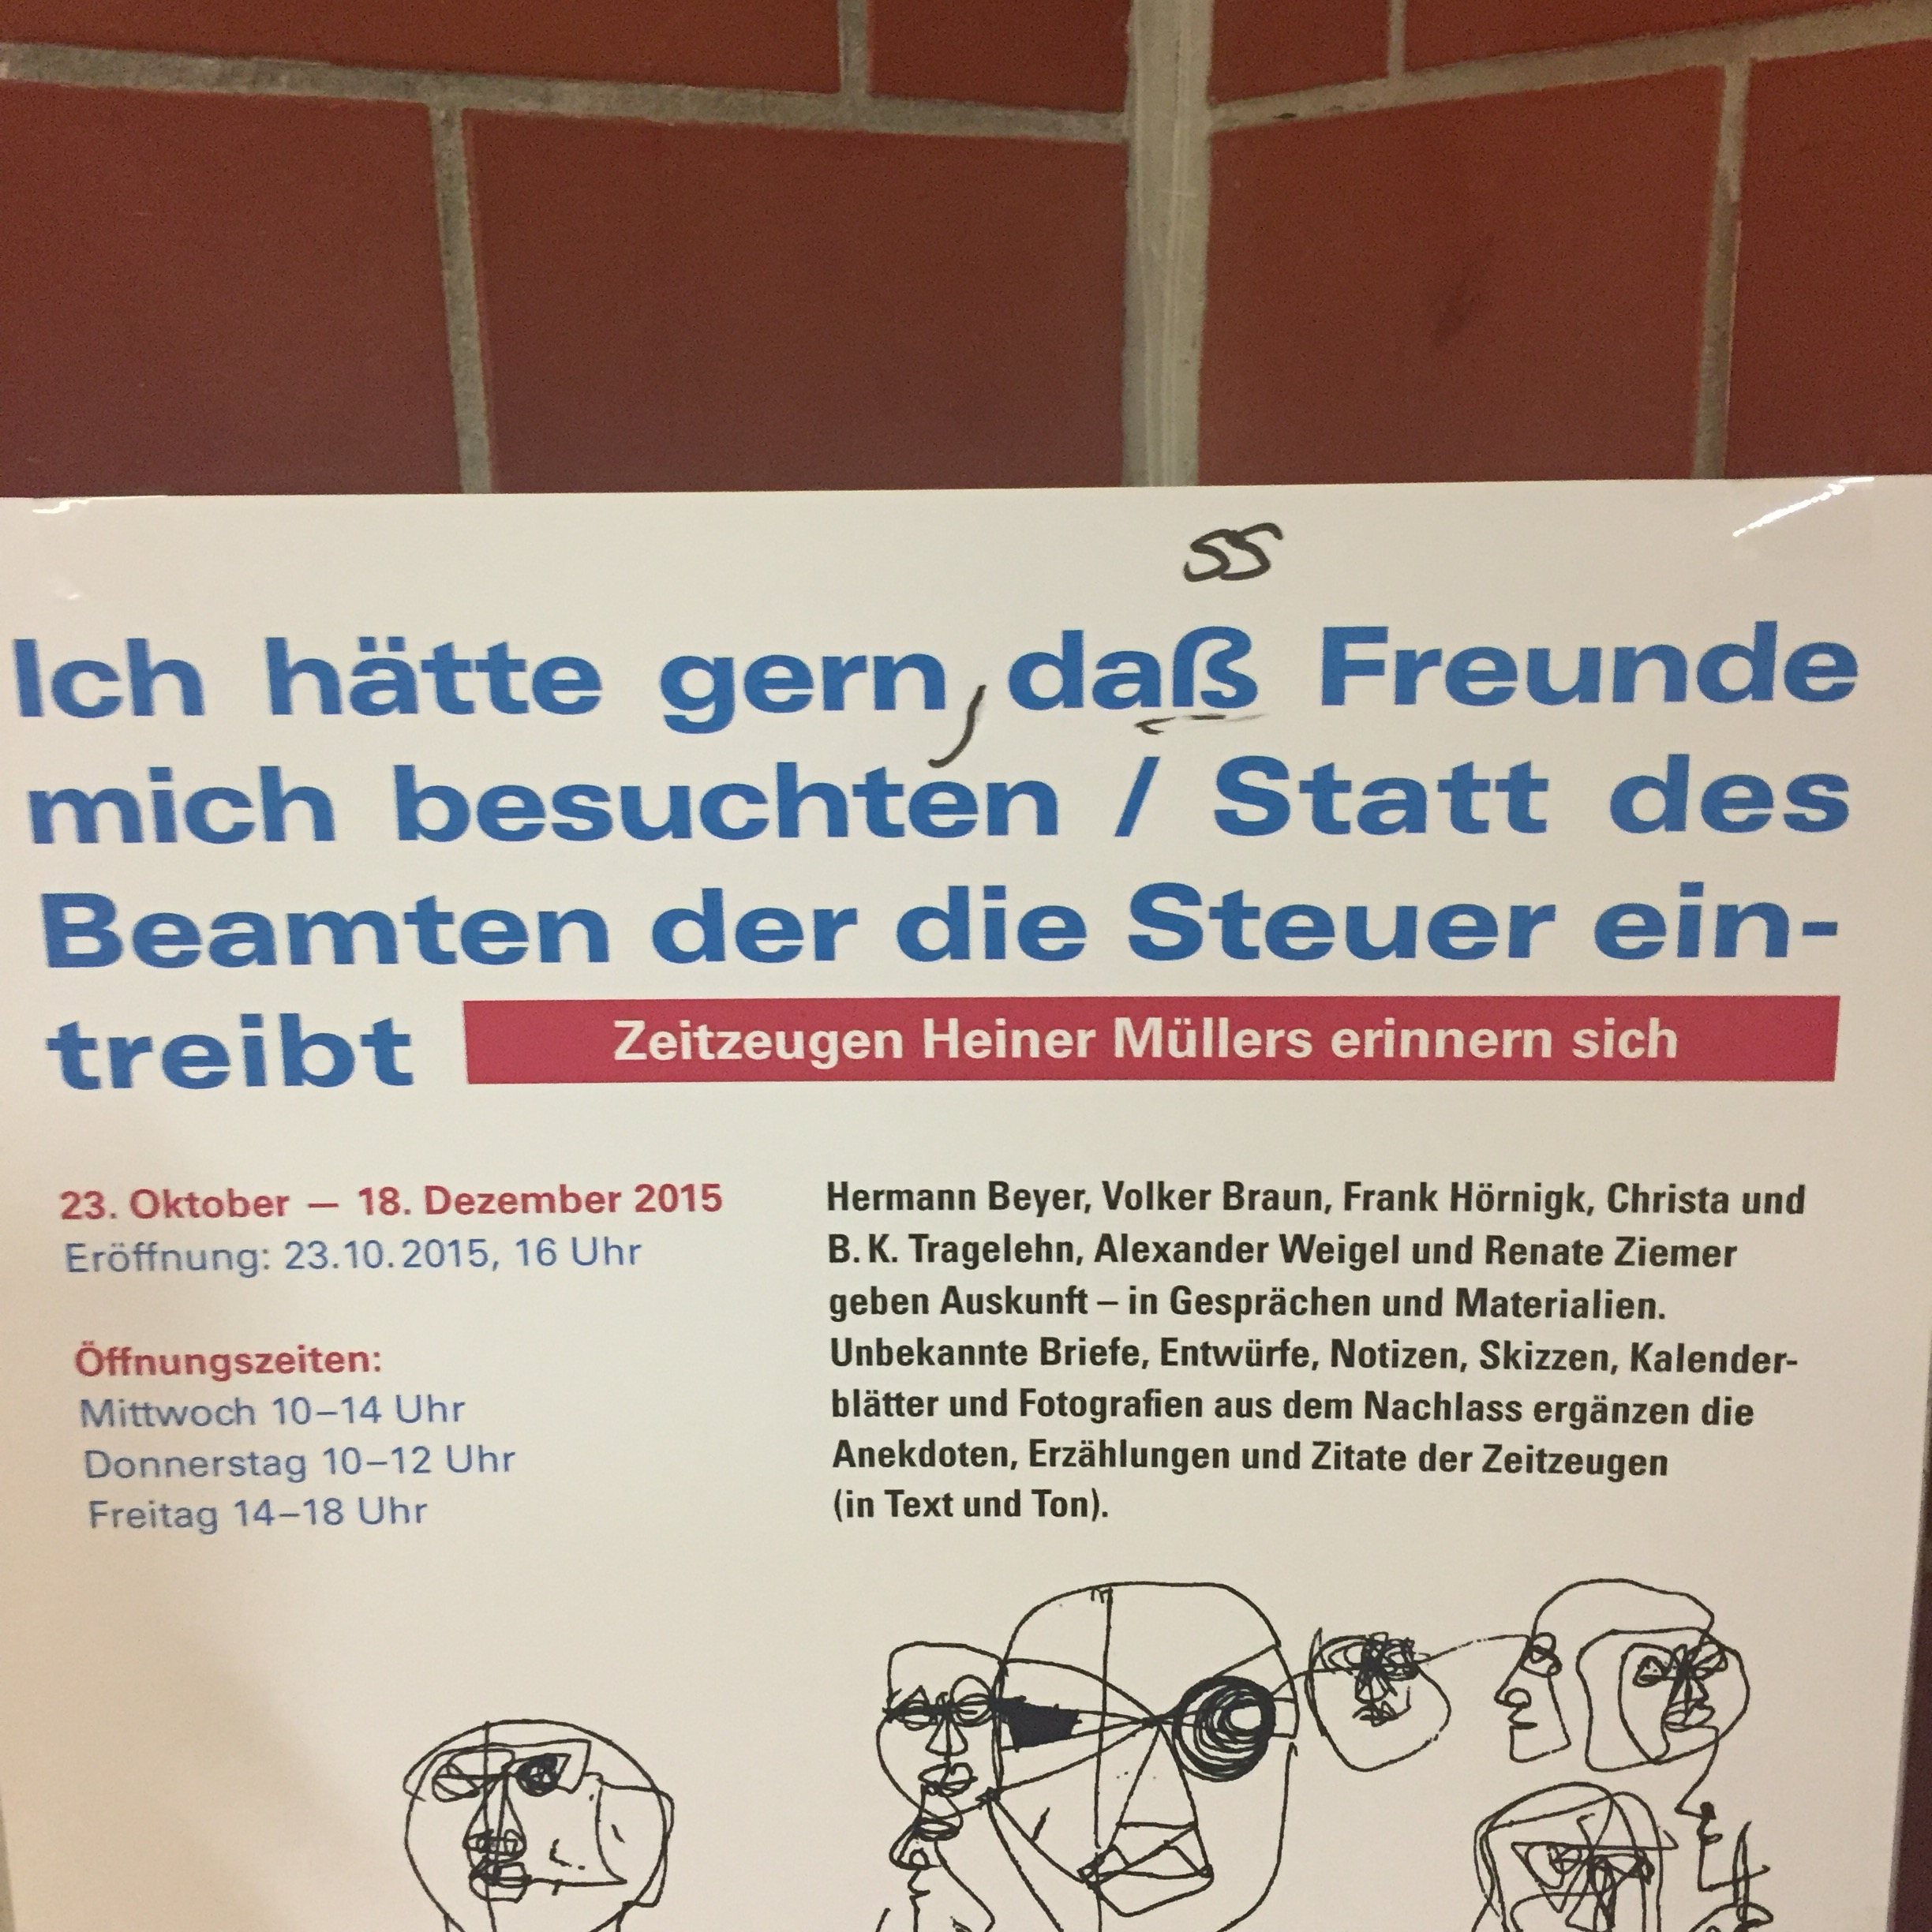
\includegraphics[scale=.065]{material/05praeskriptiv}
%	\caption{Das ist (unangemessen) präskriptiv.}\label{Abb2}
%\end{figure}
%
%\end{frame}


%%%%%%%%%%%%%%%%%%%%%%%%%%%%%%%%%%
\begin{frame}
\frametitle{Deskriptiv \vs Präskriptiv}

\begin{itemize}
	\item Arbeitsweise in der Linguistik \ras \textbf{Deskriptiv} (beschreibend)

	\item Ein Phänomen, das kompetente Sprecher produzieren, wird \textbf{beobachtet und beschrieben}. 	

\end{itemize}
	
	\ea \alertred{Gestern, ich} war im Kino und plötzlich hat es angefangen zu regnen.
	\z
	
	\ea Die theoretische Entwicklung und die praktische Programmierung solcher Betriebssysteme \alertred{hat} sich zu einem neuen Arbeitsgebiet innerhalb der Datenverarbeitung entwickelt. \hfill \citep{Goschler14a}
	\z
	


\end{frame}

%%%%%%%%%%%%%%%%%%%%%%%%%%%%%%%%%%%%%%%%%

%\begin{frame}
%	\frametitle{Deskriptiv \vs Präskriptiv}
	
%\begin{itemize}
%	\item Vorgehensweise von (einigen) Schulgrammatiken und Sprachakademien \ras \textbf{präskriptiv}

%	\item Es wird \textbf{vorgeschrieben}, wie die Strukturen der Sprache gebildet werden \gqq{müssen}.
%	\end{itemize}	
		
%	\ea Es heißt nicht \MyPobj{wegen dem Job}, sondern \MyPobj{wegen des Jobs}.	
%	\z
	
%\end{frame}


%%%%%%%%%%%%%%%%%%%%%%%%%%%%%%%%%%
\begin{frame}
	\frametitle{Deskriptiv \vs Präskriptiv}
\begin{columns}
%%
\begin{column}{.6\textwidth}

\begin{itemize}
	\item Vorgehensweise von (einigen) Schulgrammatiken und Sprachakademien \ras \textbf{präskriptiv}
	
	\medskip
	\item Es wird \textbf{vorgeschrieben}, wie die Strukturen der Sprache gebildet werden \gqq{müssen}.	

\ea Es heißt nicht \MyPobj{wegen dem Job}, sondern \MyPobj{wegen des Jobs}.	
\z

	\item präskriptive Regeln:
	
	\item[] \textbf{Stilistik} (\gqq{schöner} oder \gqq{weniger schön})\\
	oder\\
	
	\item[] Regeln für \gqq{\textbf{gutes/richtiges}} \textbf{Deutsch}
\end{itemize}


\end{column}
%%
\begin{column}{.4\textwidth}

\begin{figure}
	\centering
	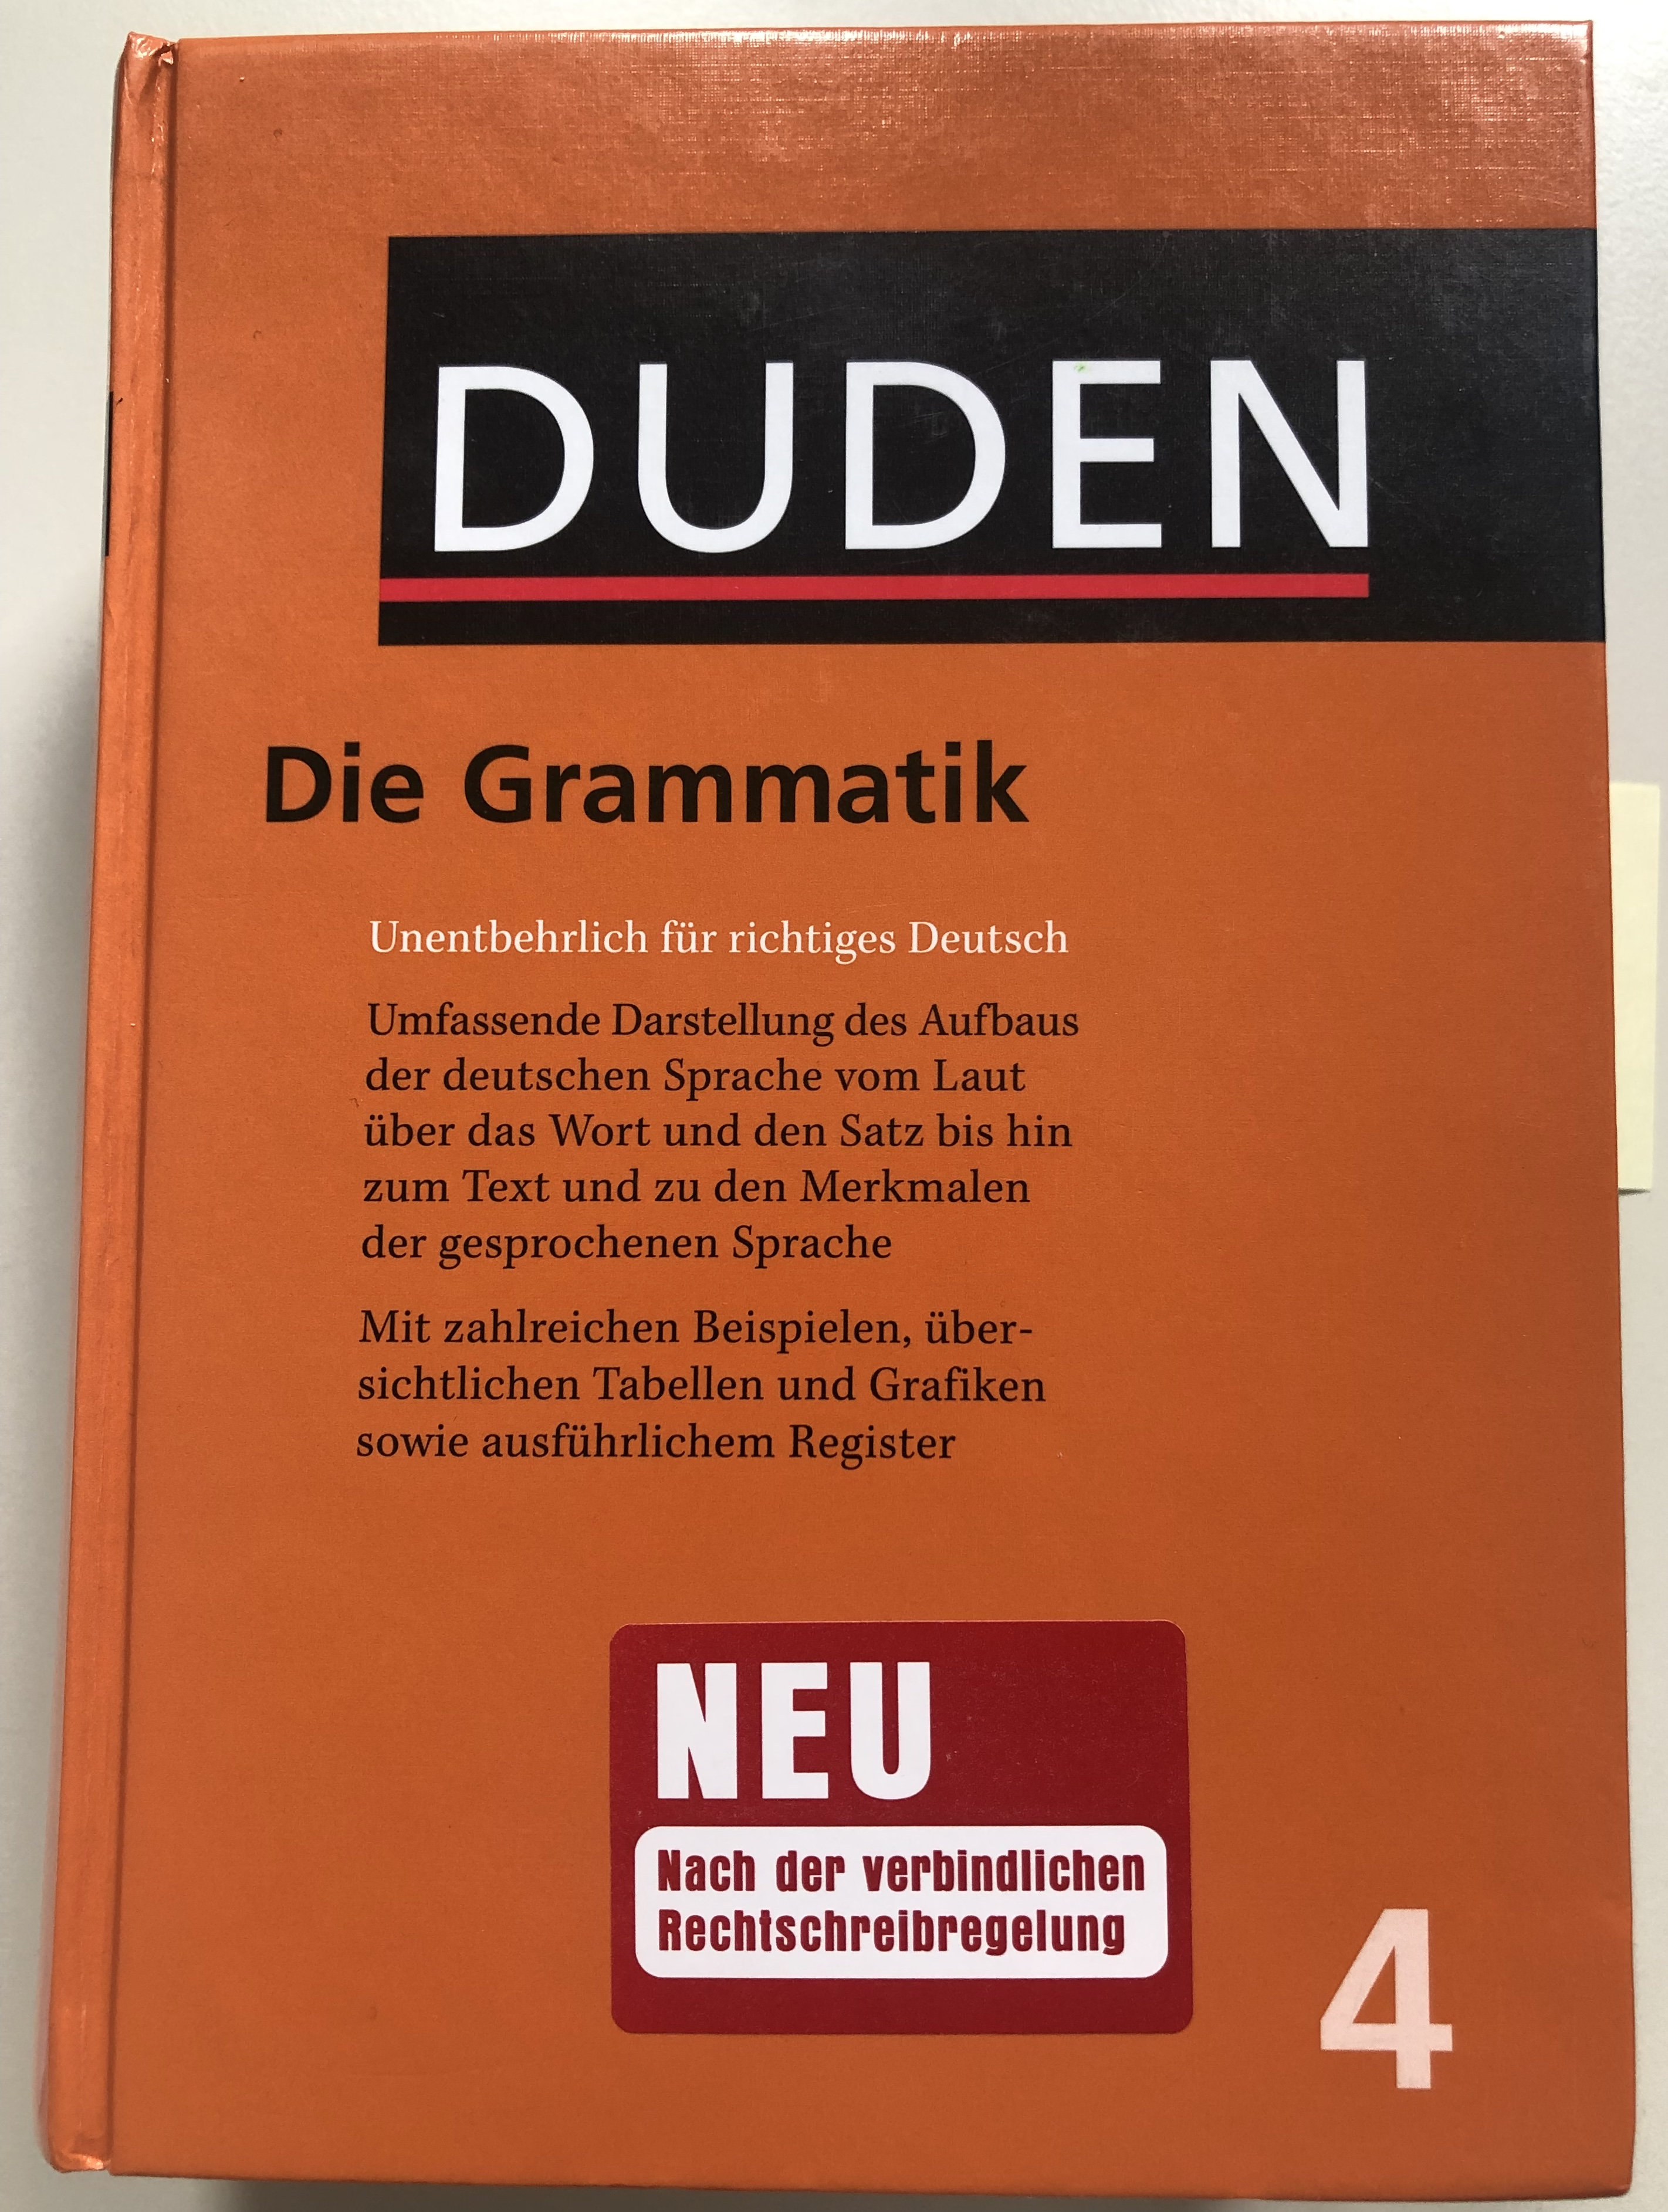
\includegraphics[scale=.045]{material/DudenRichtigesDeutsch}
	\caption{Duden \citep{DudenGramm09d}}\label{Abb3}
\end{figure}

\end{column}

\end{columns}
	
\end{frame}


%%%%%%%%%%%%%%%%%%%%%%%%%%%%%%%%%%
\begin{frame}

\begin{itemize}
%	\item Präskriptive Regeln \\
%	\ras Stilistik (\gqq{schöner} oder \gqq{weniger schön})\\
%	oder\\
%	\ras Regeln für \gqq{gutes/richtiges} Deutsch
%	\item[]
	
	\item In der Linguistik wird auf der Basis von \textbf{deskriptiven Beobachtungen} gearbeitet.
	
	\medskip
	
	\item Kompetente Sprecher verwenden ständig Formulierungen wie \MyPobj{wegen dem Job}, aber nie solche wie:
	
	\ea[*]{Ich bin \alertred{wegen der Job} gekommen.}
%	\z
	
	\ex[*]{Ich bin \alertred{dem wegen Job} gekommen.}
%	\z
	
	\ex[*]{Ich bin \alertred{wegen Job dem} gekommen.}
	\z
	
	\medskip
	\item Diese Formulierungen sind \textbf{ungrammatisch}, denn sie verletzen Regeln des deutschen \textbf{grammatischen Systems}:
	
	\begin{itemize}
		\item Präpositionen stehen \MyPobj{vor} Nominalphrasen
		\item Artikel stehen \MyPobj{vor} dem Nominalkomplex
	\end{itemize}	
	
\end{itemize}

\end{frame}


%%%%%%%%%%%%%%%%%%%%%%%%%%%%%%%%%%
%%%%%%%%%%%%%%%%%%%%%%%%%%%%%%%%%%
\subsection{Abbildungen}


%%%%%%%%%%%%%%%%%%%%%%%%%%%%%%%%%%
\begin{frame}{Abbildungen}
\small

\begin{itemize}
	%\item ABBILDUNG -- \gqq{Glowing blue binary code on screen with word error background concept} (Stock-Foto, Zugriff: 11.05.18)
	%\url{https://www.colourbox.de/bild/bild-26254540}

%	\item ABBILDUNG -- Machicao y Priemer, Antonio: \gqq{Deskriptiv vs. Präskriptiv} (Privatfoto)
	
	\item ABBILDUNG -- Machicao y Priemer, Antonio: \gqq{Duden} (Privatfoto)
\end{itemize}	

\end{frame}


%%%%%%%%%%%%%%%%%%%%%%%%%%%%%%%%%%%%%%%%%%%%%%%%
%% Compile the master file!
%% 		Slides: Antonio Machicao y Priemer
%% 		Course: GK Linguistik
%%%%%%%%%%%%%%%%%%%%%%%%%%%%%%%%%%%%%%%%%%%%%%%%

%%%%%%%%%%%%%%%%%%%%%%%%%%%%%%%%%%%%%%%%%%%%%%%%%%%%
%%%             Metadata                         
%%%%%%%%%%%%%%%%%%%%%%%%%%%%%%%%%%%%%%%%%%%%%%%%%%%%      

\title{Grundkurs Linguistik}

\subtitle{Syntax II: Einführung \& Terminologie}

\author[A. Machicao y Priemer]{
	{\small Antonio Machicao y Priemer}
	\\
	{\footnotesize \url{http://www.linguistik.hu-berlin.de/staff/amyp}}
%	\\
%	\href{mailto:mapriema@hu-berlin.de}{mapriema@hu-berlin.de}}
}

\institute{Institut für deutsche Sprache und Linguistik}

%\date{ }

%\publishers{\textbf{6. linguistischer Methodenworkshop \\ Humboldt-Universität zu Berlin}}

%\hyphenation{nobreak}


%%%%%%%%%%%%%%%%%%%%%%%%%%%%%%%%%%%%%%%%%%%%%%%%%%%%
%%%             Preamble's End                  
%%%%%%%%%%%%%%%%%%%%%%%%%%%%%%%%%%%%%%%%%%%%%%%%%%%%      


%%%%%%%%%%%%%%%%%%%%%%%%%      
\huberlintitlepage[22pt]

\iftoggle{toc}{
\frame{
\begin{multicols}{2}
	\frametitle{Inhaltsverzeichnis}\tableofcontents
	%[pausesections]
\end{multicols}
	}
	}


%%%%%%%%%%%%%%%%%%%%%%%%%%%%%%%%%%
%%%%%%%%%%%%%%%%%%%%%%%%%%%%%%%%%%
%%%%%LITERATURE:

%% Allgemein
\nocite{Glueck&Roedel16a}
\nocite{Grewendorf&Co91a} 
\nocite{Luedeling2009a} 
\nocite{Meibauer&Co07a} 
\nocite{Repp&Co15a} 

%% Morphologie
%\nocite{Eisenberg04}

%% Syntax
\nocite{Adger04a}
%\nocite{Altmann&Hofmann08a} % Satztypen & Satzmodi
%\nocite{Altmann93a} % Satztypen & Satzmodi
\nocite{Brandt&Co06a} 
\nocite{Fries&MyP16b} % Akzeptabilität
\nocite{Fries16a} % Grammatikalität
\nocite{Fries&MyP16d} % Kompetenz vs Performanz
\nocite{Fries&MyP16c} % GG
\nocite{Fries&MyP16a} % X-Bar-Theorie
%\nocite{Fries16e} % Satztyp
%\nocite{Fries16d} % Satzmodus 
\nocite{Grewendorf&Co91a} 
\nocite{MyP17b} % Kerngrammatik
\nocite{MyP18a} % Konstituententest
\nocite{MyP18b} % Kopf
\nocite{MyP18c} % Phrase
\nocite{MyP18g} %Entscheidungsfragesatz
\nocite{MyP18i} %Ergänzungsfragesatz
\nocite{MuellerS13f} 
\nocite{MuellerS15b}
\nocite{Stechow&Sternefeld88a}
%\nocite{Sternefeld06a}
%\nocite{Sternefeld06b}
%\nocite{Woellstein10a} % Topologisches Feldermodell

%%%%%%%%%%%%%%%%%%%%%%%%%%%%%%%%%%

\begin{frame}
	\frametitle{Begleitlektüre}
		\begin{itemize}
			\item \textbf{obligatorisch:}
				\begin{itemize}
					\item[] \citet{MyP18a}
				\end{itemize}
			\end{itemize}
		
			\begin{block}{Lektüre für die vorlesungsfreie Zeit}
			\begin{itemize}
				\item \textbf{obligatorisch:}	
				\begin{itemize}	
					\item[] \citet{Woellstein10a}: Kapitel 2 \& 3 (S. 20--53)
					\item[] \citet{MyP18c}
				\end{itemize}
				\item \textbf{optional:}
					\begin{itemize}
						\item[] \citet{Brandt&Co06a}: Kapitel 5--9 (S. 26--65)
					\end{itemize}	
				\end{itemize}
		\end{block}
	
\end{frame}

%%%%%%%%%%%%%%%%%%%%%%%%%%%%%%%%%%
\section{Syntax II: Einführung und Terminologie}

%%%%%%%%%%%%%%%%%%%%%%%%%%%%%%%%%%
\subsection{Was bisher geschah \dots }

\iftoggle{sectoc}{
	\frame{
		%\begin{multicols}{2}
		\frametitle{~}
		\tableofcontents[currentsubsection,subsubsectionstyle=hide]
		%\end{multicols}
	}
}


%%%%%%%%%%%%%%%%%%%%%%%%%%%%%%%%%%
\begin{frame}
\frametitle{Was bisher geschah \dots }

%\begin{itemize}
%	\item 
	Sie wissen bereits:
	
	\begin{itemize}
		\item \textbf{womit} sich die Syntax befasst,
		\item wie man Syntax \textbf{definieren} kann,
		\item dass man auch \textbf{Konstituenten} und \textbf{Kategorien} einbeziehen muss,
		\item dass \textbf{Linearität} $\neq$ \textbf{Struktur},
		\item was der Unterschied zwischen \textbf{Grammatikalität} und \textbf{Akzeptabilität} ist,
		\item was der Unterschied zwischen \textbf{deskriptiv} und \textbf{präskriptiv} ist.
	\end{itemize}
%\end{itemize}

\end{frame}


%%%%%%%%%%%%%%%%%%%%%%%%%%%%%%%%%%
%%%%%%%%%%%%%%%%%%%%%%%%%%%%%%%%%%
\subsection{Generative Grammatik}

\iftoggle{sectoc}{
	\frame{
		%\begin{multicols}{2}
		\frametitle{~}
		\tableofcontents[currentsubsection,subsubsectionstyle=hide]
		%\end{multicols}
	}
}


%%%%%%%%%%%%%%%%%%%%%%%%%%%%%%%%%%
\begin{frame}
\frametitle{Generative Grammatik}

\begin{minipage}[c]{0.57\textwidth}
\begin{itemize}
	\item<1-> Wie gelangen wir zu den deskriptiven Regeln, um die (Un-)Grammatikalität innerhalb eines Regelapparats zu modellieren?

%\pause

	\medskip
	\item<2->  \textbf{Sprachliche Intuition}: \textbf{Sprecher} haben ein \textbf{Gefühl} dafür, was sie in ihrer Muttersprache sagen können und was nicht.
	
	Durch \textbf{Introspektion} (Selbstbefragung) gelangen sie zu diesem Wissen. Dadurch befragen sie ihre sog.\ \textbf{muttersprachliche Kompetenz}.
	
%\pause
	
	\medskip 
	\item<3-> Sprachliche Intuition: wesentlich in den sog.\ generativen Syntaxtheorien seit \citet{Chomsky57x}
	

\end{itemize}
\end{minipage}
%%
%%
\begin{minipage}[c]{0.40\textwidth}

\begin{figure}
	\centering
\only<1->{	
	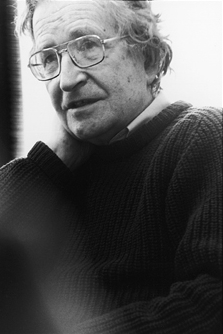
\includegraphics[scale=.5]{material/chomsky01}\label{Abb1}
}
\end{figure}

\end{minipage}

\end{frame}


%%%%%%%%%%%%%%%%%%%%%%%%%%%%%%%%%%
%\begin{frame}
%\frametitle{Generative Grammatik}
%
%\begin{itemize}
%
%	\item Sprachliche Intuition \ras wesentlich in den sog. generativen Syntaxtheorien seit \citet{Chomsky57x}
%
%\begin{figure}
%\centering
%	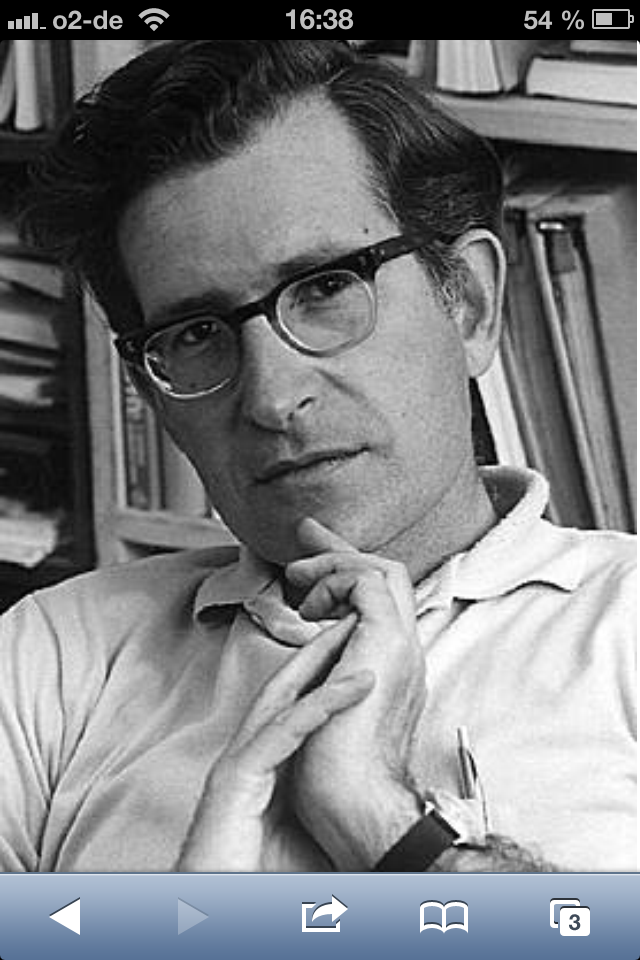
\includegraphics[scale=.17]{material/03chomsky}
%\end{figure}
%
%	
%\end{itemize}
%
%\end{frame}


%%%%%%%%%%%%%%%%%%%%%%%%%%%%%%%%%%
%\begin{frame}
%\frametitle{Generative Grammatik}


%\begin{itemize}
	
%	\item Sprachliche Intuition: wesentlich in den sog.\ generativen Syntaxtheorien seit \citet{Chomsky57x}
		
%\end{itemize}


%\begin{figure}
%	\centering
%	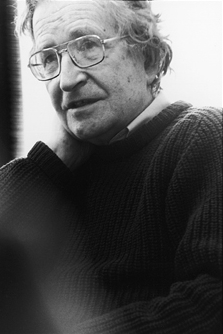
\includegraphics[scale=.5]{material/chomsky01}\label{Abb1}
%\end{figure}

%\end{frame}


%%%%%%%%%%%%%%%%%%%%%%%%%%%%%%%%%%
\begin{frame}
\frametitle{Generative Grammatik}

\begin{itemize}
	\item Was ist diese Generative Grammatik (GG)? 
	\medskip
	\item Seit \citet{Chomsky57x} und \citet{Chomsky65a}
	\medskip
	\item \textbf{dynamische Theorie} (vgl.\ statische Theorie \ras \zB Strukturalismus)
	\begin{itemize}
		\item Grammatik als dynamisches System: Regelsystem, das wohlgeformte Strukturen \emph{erzeugt}
		\medskip
		\item Strukturalistisches Konzept \gqq{Langue} setzt ein statisches Zeichensystem voraus. 
	\end{itemize}

\end{itemize}

\end{frame}


%%%%%%%%%%%%%%%%%%%%%%%%%%%%%%%%%%
\begin{frame}
\frametitle{Generative Grammatik}

\begin{itemize}
	\item Klare Definition des Untersuchungsgegenstandes \gqq{Sprache}:
	\begin{itemize}
		\item Keine Beschreibung mehr von \gqq{sprachlichen} Phänomenen, ohne davor den Begriff \gqq{Sprache} zu definieren / einzuschränken.
		\medskip
		\item \textbf{I-Language} \ras intrinsische Kompetenz des idealen Sprecher"=Hörers (Trennung zwischen Kompetenz und Performanz)
	\end{itemize}
	\medskip
	\item Linguistik als Wissenschaft \ras durch Formalisierung
	\medskip
	\item \textbf{Rationalistische} Vorgehensweise (Cartesianische Linguistik)
	\begin{itemize}
		\item Bruch mit behavioristischer Vorgehensweise (Empirismus)
		\item Rationalistische Sichtweise des Spracherwerbs
		\item Universalgrammatik \ras genetisch verankerte Grundlage der menschlichen Sprachfähigkeit
	\end{itemize}
\end{itemize}

\nocite{Fries&MyP16d}

\end{frame}


%%%%%%%%%%%%%%%%%%%%%%%%%%%%%%%%%%
\begin{frame}
\frametitle{Generative Grammatik}

\begin{itemize}
	\item Verwandtschaft zwischen Sätzen erkennen, beschreiben und erklären (Erklärungsadäquatheit) \ras Transformationen
	
	\eal 
	\ex Man kauft Bier.
	\ex Bier wird gekauft.
	\zl
	
	\medskip	
	\item Beschreibung von sprachlichen Phänomenen ist nicht das primäre Ziel.
\end{itemize}

\end{frame}


%%%%%%%%%%%%%%%%%%%%%%%%%%%%%%%%%%
\begin{frame}
\frametitle{Generative Grammatik}

\begin{block}{Ziel generativer Theorien}
Durch eine \textbf{deskriptive} Vorgehensweise wird ein Regelapparat erstellt, um \textbf{lineare} und \textbf{hierarchische} Gesetzmäßigkeiten des Satzbaus zu \textbf{beschreiben}. Daraus wird versucht, allgemeine (\textbf{universelle}) Gesetzmäßigkeiten der menschlichen Sprachfähigkeit abzuleiten, um somit die menschliche (Sprach)\textbf{Kompetenz zu erklären}.
\end{block}

\end{frame}


%%%%%%%%%%%%%%%%%%%%%%%%%%%%%%%%%%
%%%%%%%%%%%%%%%%%%%%%%%%%%%%%%%%%%
\subsubsection{Kompetenz \vs Performanz}

%\iftoggle{sectoc}{
%	\frame{
%		\begin{multicols}{2}
%		\frametitle{~}
%		\tableofcontents[currentsubsection,subsubsectionstyle=hide]
%		\end{multicols}
%	}
%}


%%%%%%%%%%%%%%%%%%%%%%%%%%%%%%%%%%
\begin{frame}
\frametitle{Kompetenz \vs Performanz}

\begin{block}{Kompetenz (Sprachfähigkeit)}
Ein mental (\gqq{im Geist}) verankertes \textbf{unbewusstes Wissenssystem von Regeln}, das der Produktion und Rezeption unendlich vieler Sätze zugrunde liegt (auch: I-Sprache für internalisierte Sprache) \citep[vgl.][]{Fries&MyP16d}.
\end{block}	


\end{frame}


%%%%%%%%%%%%%%%%%%%%%%%%%%%%%%%%%%
\begin{frame}
\frametitle{Kompetenz \vs Performanz {\footnotesize \citep[vgl.][16ff.]{Brandt&Co06a}}}

\begin{itemize}
	\item Die Kompetenz äußert sich in der Fähigkeit:

	\begin{itemize}
		\medskip
		\item Sätze einer Sprache als \textbf{grammatisch oder ungrammatisch} zu beurteilen,

\pause		
\only<2>{
		\ea \alertred{Peter$_i$} rasiert \{\alertred{*ihn$_i$/sich$_i$}\}.
		\z
		
		\ea \alertred{Peter$_i$} freut sich, dass man \{\alertred{ihn$_i$/*sich$_i$}\} gelobt hat.
		\z
		}

\pause	
		\medskip	
		\item \textbf{strukturell verwandte} Sätze zu erkennen,
\pause
\only<4>{
		\ea Man kauft ein Haus.
		\z
		
		\ea Ein Haus wird gekauft.
		\z
		}

\pause	
		\medskip	 
		\item \textbf{strukturelle und lexikalische Ambiguitäten} zu erkennen,
\pause
\only<6>{
		\ea Peter traf \alertred{die Frau mit dem roten Schuh}.
		\z
		
		\ea Peter liebt die \alertred{Schule}.
		\z
		}

\pause	
		\medskip	 
		\item \textbf{syntaktisch wohlgeformte Äußerungen} zu erkennen, auch wenn der Inhalt unsinnig ist.
\pause
\only<8>{
		\ea[]{Viele hartnäckig verheiratete Junggesellen stehen intensiv.}
		\z
		
		\ea[*]{Hartnäckig intensiv Junggesellen stehen verheiratete viele.}
		\z
		}
		
	\end{itemize}
\end{itemize}
\end{frame}


%%%%%%%%%%%%%%%%%%%%%%%%%%%%%%%%%%%
%\begin{frame}
%\frametitle{Kompetenz \vs Performanz (Ambiguität)}
%
%%\begin{figure}
%%\centering
%%	
\includegraphics[scale=.5]{material/08ambiguity}
%%	\caption{Ambiguität}
%%\end{figure}
%
%{\LARGE
%
%I'm a linguist.
%
%\vspace{2em}
%
%I love ambiguity more than most people.}
%
%
%\end{frame}


%%%%%%%%%%%%%%%%%%%%%%%%%%%%%%%%%%
\begin{frame}
\frametitle{Kompetenz \vs Performanz}

\begin{block}{Performanz (Sprachverwendung)}
Anwendung der Sprachfähigkeit in einer konkreten Sprechsituation \citep[vgl.][]{Fries&MyP16d}	
\end{block}

\end{frame}


%%%%%%%%%%%%%%%%%%%%%%%%%%%%%%%%%%
\begin{frame}

Die Performanz weicht oft von der Kompetenz ab: 
	\begin{itemize}
		\item Sprecher versprechen sich, 
		
\pause		
%\only<2>{
		\ea Ich hätte gerne einen \alertred{K}ilch\alertred{m}affee\dots\ Ähm! Ich meine einen \alertred{M}ILCH\alertred{K}affee.
		\z
%		}

\pause	
		\item brechen mitten im Satz ab,
\pause		
%\only<4>{
		\ea Ich wollte ja noch \alertred{\dots } Ach, nichts!
		\z
%		}

		\item wiederholen Wörter.
\pause		
%\only<6>{
		\ea \alertred{Ich hab ich hab ich hab} gestern noch den Film geguckt.
		\z
%		}

		\item[]	Aber niemand würde daraus schließen, dass sie ihre Muttersprache nicht beherrschen.
	\end{itemize}

\end{frame}


%%%%%%%%%%%%%%%%%%%%%%%%%%%%%%%%%%
\begin{frame}

\begin{itemize}

	\item Die Unterscheidung grammatisch"=ungrammatisch spiegelt die Kompetenz des \textbf{idealen Sprecher"=Hörers} wider.
	\begin{itemize}
		\item [\ras] \textbf{Idealer Sprecher"=Hörer:}\\
			Theoretisches (und nicht unumstrittenes) Konstrukt innerhalb der Generativen Grammatik, um die Sprachdaten, mit denen gearbeitet wird, von \gqq{Performanzeffekten zu bereinigen}. Notwendig für eine Abgrenzung des Untersuchungsgegenstandes der GG \citep[vgl.][]{Fries16b}.
	\end{itemize}
\item []
	\item Die verschiedenen Akzeptabilitätsgrade haben häufig mit Performanzeffekten zu tun.
	\item []
	\item Die Kompetenz"=Performanz"=Dichotomie wird in einigen (gebrauchsbasierten) Frameworks (\zB Construction Grammar) abgelehnt \citep[vgl.][]{MuellerS15b, Nolda&Co14a}. 
\end{itemize}

\end{frame}


%%%%%%%%%%%%%%%%%%%%%%%%%%%%%%%%%%
%%%%%%%%%%%%%%%%%%%%%%%%%%%%%%%%%%
\subsubsection{Universalgrammatik}

%\iftoggle{sectoc}{
%	\frame{
%		\begin{multicols}{2}
%		\frametitle{~}
%		\tableofcontents[currentsubsection,subsubsectionstyle=hide]
%		\end{multicols}
%	}
%}

%%%%%%%%%%%%%%%%%%%%%%%%%%%%%%%%%%%
\begin{frame}
\frametitle{Universalgrammatik (UG)}

\begin{itemize}

	\item Die (menschliche) natürliche Sprache unterscheidet sich von der Sprache anderer Tiere in vielerlei Hinsicht \citep[vgl. \zB][]{Hockett60a-removed, Pinker95a}.\\
	(Gegenargumente und Diskussion: \citealt{Evans&Levinson09a, MuellerS15b})
	\medskip
	\item Welche Merkmale unterscheiden eine \textbf{natürliche Sprache} von anderen Sprachen? 
	\begin{itemize}
		\item Produktivität, Bidirektionalität, Arbitrarität, Diskretheit, Rekursivität, \dots \\
		\citep[vgl.][]{Hockett60a-removed, Luedeling2009a}
	\end{itemize}

%	Syntax von Vögeln! 

	\medskip
	\item Andere Primaten können bspw. lexikalische Einträge erwerben (25--125 lexikalische Einträge), aber \textbf{keine abstrakten Regeln}.
\end{itemize}

\end{frame}


%%%%%%%%%%%%%%%%%%%%%%%%%%%%%%%%%%
\begin{frame}
%\frametitle{Universalgrammatik}

\begin{figure}
\centering
	\includegraphics[scale=.26]{material/schimpansen}
	\caption{Schimpansen}
\end{figure}

\begin{itemize}
	\item Siehe \textbf{Nim Chimpsky}: \url{https://en.wikipedia.org/wiki/Nim_Chimpsky}

	\ea Give orange me give eat orange me eat orange give me eat orange give me you. \hfill (Nim Chimpsky)
	\z
\end{itemize}


\end{frame}


%%%%%%%%%%%%%%%%%%%%%%%%%%%%%%%%%%
\begin{frame}

\begin{itemize}
	\item \textbf{Erwerbbarkeit} von Regeln 
	\begin{itemize}
		\item Dem Kind muss es möglich sein, \textbf{abstrakte Regeln} zu erwerben.
		\medskip
		\item Mit welcher Sprachausstattung kommt das Kind zur Welt? \ras UG
		\medskip
		\item Wie müssen Regeln aussehen, damit sie mit dieser angeborenen Sprachausstattung (UG) erworben werden können?
		\medskip
		\item \textbf{Mentalistischer Nativismus} in der \textbf{rationalistischen} Tradition von Descartes und Humboldt (vs. empiristische Tradition) \ras Große Bereiche kognitiver Strukturen sind \textbf{genetisch} vorgegeben (vgl.\ Biolinguistik \ras FOXP2) \citep[vgl.][]{Hornstein05a}.
		\medskip
		\item Angeborene Sprachausstattung \ras Set von Prinzipien \ras UG		
	\end{itemize}
\end{itemize}

\end{frame}


%%%%%%%%%%%%%%%%%%%%%%%%%%%%%%%%%%
\begin{frame}

\begin{itemize}
	\item \textbf{Argument vom defizienten Input} (Poverty-of-the-Stimulus Argument) beim Spracherwerb:
	
	\begin{itemize}
		\item Das Kind bekommt nur sog. positive Evidenz beim Erlernen \ras aber nur Performanzdaten!
		\medskip
		\item Vorkommen von Fehlern
		\medskip
		\item Korrekturen \ras nicht bei jeder falschen Äußerung
		\medskip
		\item Unterschiedliche Leute korrigieren unterschiedlich
		\medskip
		\item Trotzdem lernen alle Kinder ihre Muttersprache auf dieselbe Art und Weise in ungefähr der gleichen Zeit \citep[vgl.][18ff.]{Philippi&Tewes10a}.
		\medskip
		\item Das deutet daraufhin, dass das Kind schon mit einer gewissen Sprachkompetenz (Set sprachlicher Prinzipien oder UG) geboren wird.

	\end{itemize}

\end{itemize}

\end{frame}


%%%%%%%%%%%%%%%%%%%%%%%%%%%%%%%%%%
\begin{frame}

\begin{itemize}
	\item \textbf{Argument vom defizienten Input} (Poverty-of-the-Stimulus Argument) beim Spracherwerb (vgl. \citealt{Lasnik&Co02a} vs. \citealt{Pullum&Scholz02a}):
	\medskip
	\item Prinzip der \textbf{Strukturabhängigkeit:}
	\eal 
	\ex[]{Der Hund \alertred{ist} hungrig.}
\pause
	\ex[]{\alertred{Ist} der Hund hungrig?}
\pause
	\ex[]{Der Hund, der an der Ecke \alertred{ist}, \alertred{ist} hungrig.}
\pause	
	\ex[*]{\alertred{Ist}$_{i}$ der Hund, der an der Ecke \alertred{t}$_{i}$, \alertred{ist} hungrig?}
\pause
	\ex[]{\alertred{Ist}$_{i}$ der Hund, der an der Ecke \alertred{ist}, \alertred{t}$_{i}$ hungrig?}
	\zl

\pause	

	\eal 
	\ex \alertred{Er}$_{\neq 1, =2}$ hat gesagt, dass \alertred{Peter}$_1$ Maria mag.
\pause	
	\ex \alertred{Peter}$_1$ hat gesagt, dass \alertred{er}$_{=1, =2}$ Maria mag.
\pause	
	\ex Dass \alertred{er}$_{=1, =2}$ Maria mag, hat \alertred{Peter}$_1$ gesagt.
	\zl
	
	
\end{itemize}

\end{frame}


%%%%%%%%%%%%%%%%%%%%%%%%%%%%%%%%%%
\begin{frame}
\frametitle{Universalgrammatik}

\begin{itemize}
	\item \textbf{Kreativitätsargument}
	\medskip
	\item Mit einer \textbf{begrenzten Anzahl an Phonemen}, kann man eine \textbf{begrenzte Anzahl an Wörtern} generieren, mit denen man aber \textbf{eine unendliche Menge an Sätzen} produzieren und verstehen kann.

\pause	
	\ea Karl-Heinrich hat trotz seiner Seekrankheit genügend Argumente, um für die bessere Behandlung der Flüchtlinge in seinem Bezirk zu demonstrieren.
	\z

\end{itemize}

\end{frame}


%%%%%%%%%%%%%%%%%%%%%%%%%%%%%%%%%%
\begin{frame}
\frametitle{Universalgrammatik}

\begin{itemize}
	\item \textbf{Argument der Übergeneralisierung}
	\medskip
	\item Fehler von Kindern weisen auf die Anwendung von Regeln hin (Übergeneralisierung).

\pause	
	\eal 
	\ex geben
	\ex gegebt
	\zl
	
	\eal 
	\ex A: Schläfst du?
	\ex B: Ja, ich schläfe.
	\zl
	
	\eal 
	\ex das Schaf
	\ex die Schäfe (vgl. der Ball -- die Bälle)
	\zl

\end{itemize}

\end{frame}


%%%%%%%%%%%%%%%%%%%%%%%%%%%%%%%%%%
\begin{frame}

\begin{itemize}
	\item Unterschiedliche Sprachen auf der Welt aber nur \textbf{eine UG}? \ras \textbf{Prinzipien vs. Parameter}

	\begin{block}{Prinzipien}
	Universelle Regeln, nach denen mögliche Sprachen gebildet werden und unmögliche ausgeschlossen werden. 
	\end{block}
	
	\item \textbf{Kopfprinzip:} Jede Phrase hat einen und nur einen Kopf.

\pause
	\eal 
	\ex[]{[Kekse$_ {N}$ backen$_ {V}$]$_ {VP}$}
	\ex[*]{[Kekse$_ {N}$ backen$_ {V}$]$_ {NP}$}
	\ex[*]{[Kekse$_ {N}$ backen$_ {V}$]$_ {VP \& NP}$}
	\zl
	
\end{itemize}

\end{frame}


%%%%%%%%%%%%%%%%%%%%%%%%%%%%%%%%%%
\begin{frame}

\begin{itemize}

	\begin{block}{Parameter}
	Einzelsprachlich spezifische Regeln, die Möglichkeiten darstellen, die universalgrammatischen Prinzipien auszubuchstabieren.
	\end{block}
	
	\item Durch den Input der Zielsprache werden sog.\ \textbf{Parameter} gesetzt.
	\medskip
	\item \textbf{Kopfparameter:} Position des Kopfes einer Phrase (vgl. Prinzip der Rechtsköpfigkeit in der Morphologie)
	
	\eal
	\ex Dt.: das grüne \alertred{Haus}
	\ex
	\gll Sp.: la \alertred{casa} verde\\
		{} das Haus grün\\
	\zl
	
	\item Ein Adjektiv kann in einer Nominalphrase in Abhängigkeit von der jeweiligen Sprache links oder rechts vom Nomen stehen.


\end{itemize}

\end{frame}


%%%%%%%%%%%%%%%%%%%%%%%%%%%%%%%%%%
\begin{frame}

\begin{itemize}
	\item Inventar an Prinzipien und Parametern ist beschränkt (aus Ökonomiegründen).
	\item Prinzipien und Parameter sind Teil unserer grammatischen Kompetenz.
	\medskip
	\item \textbf{Kerngrammatik} $=$ UG $+$ sprachspezifische Parameter
	\item \textbf{Einzelgrammatik} $=$ Kerngrammatik $+$ Peripherie
	\medskip
	\item Peripherie: Entlehnungen, historische Residuen, Erfindungen, Ausnahmen \citep[vgl.][]{Nolda&Co14a}
	\eal
	\ex sterben -- starb -- gestorben
	\ex Forelle blau
	\ex sitt (\url{https://de.wikipedia.org/wiki/Sitt})
	\ex In den Müll damit! \citep[vgl.][]{MuellerG11a}
	\zl
	
\end{itemize}

\nocite{MyP17b}
\nocite{MyP&Co14b}

\end{frame}


%%%%%%%%%%%%%%%%%%%%%%%%%%%%%%%%%%
\begin{frame}
\frametitle{Universalgrammatik}

\begin{block}{Ziel generativer Theorien}
In einer \textbf{deskriptiven} Vorgehensweise werden Phänomene adäquat \textbf{beobachtet} und deren \textbf{lineare} und \textbf{hierarchische} Regelmäßigkeiten adäquat \textbf{beschrieben}, dabei werden die \textbf{Performanz}phänomene und die Elemente der \textbf{Peripherie} aus der Untersuchung ausgeschlossen. Aus den Phänomenen der \textbf{Kerngrammatik} wird versucht, allgemeine (\textbf{universelle}) Gesetzmäßigkeiten der menschlichen Sprachfähigkeit abzuleiten (\textbf{Prinzipien und Parameter \ras UG}), um somit die menschliche (Sprach)\textbf{Kompetenz} zu \textbf{erklären} \citep[vgl.][]{Fries16c}.
\end{block}

Schlagen Sie \gqq{Adäquatheit} in \citet{Glueck&Roedel16a} nach!

\end{frame}


%%%%%%%%%%%%%%%%%%%%%%%%%%%%%%%%%%
%%%%%%%%%%%%%%%%%%%%%%%%%%%%%%%%%%
\subsection{Wortarten}

\iftoggle{sectoc}{
	\frame{
%		\begin{multicols}{2}
		\frametitle{~}
		\tableofcontents[currentsubsection,subsubsectionstyle=hide]
%		\end{multicols}
	}
}

%%%%%%%%%%%%%%%%%%%%%%%%%%%%%%%%%%
\begin{frame}
\frametitle{Wortarten}

\begin{itemize}
	\item \textbf{Klassifikation} des Wortschatzes unter grammatischen Gesichtspunkten 
	\medskip

\pause	

	\ea Raustorf\visible<3->{\alertred{\MyPdown{N}}} ergt\visible<4->{\alertred{\MyPdown{V}}} schrubbenes\visible<5->{\alertred{\MyPdown{A}}} Klot\visible<6->{\alertred{\MyPdown{N}}}.
	\z

\medskip
\visible<7->{
	\item \textbf{Semantische Klassifikation}:
	\begin{itemize}
		\item Elemente, die auf \textbf{Entitäten} referieren \ras Substantive
		\item Elemente, die auf \textbf{Eigenschaften} referieren \ras Adjektive
		\item Elemente, die eine \textbf{Handlung} ausdrücken \ras Verben

	\end{itemize}
}

\medskip
\visible<8->{
\begin{itemize}	
	\item Kriterien für die Klassifikation \ras \textbf{morphologisch, syntaktisch, semantisch, (pragmatisch)}
	
\end{itemize}
}

\end{itemize}

\end{frame}


%%%%%%%%%%%%%%%%%%%%%%%%%%%%%%%%%%
\begin{frame}
\frametitle{Wortarten}

\begin{itemize}
	\item Klassifikation von Wörtern in Oberkategorien \ras bereits in der klassischen griechischen Grammatik
	\medskip
	\item Wortartenklassifikation von Dionysius Thrax (200--100 v.\ Chr.):
\pause
	\begin{itemize}
		\item Nomen,
		\item Verb, 
		\item Pronomen,
		\item Präposition,
		\item Adverb,
		\item Konjunktion,
		\item Partizip,
		\item Artikel,
	\end{itemize}
\pause
	\begin{itemize}
		\item Adjektiv,
		\item Partikeln,
		\item Interjektionen, \dots
	\end{itemize}
\end{itemize}

\nocite{Thrax74a}

\end{frame}


%%%%%%%%%%%%%%%%%%%%%%%%%%%%%%%%%%
\begin{frame}
\frametitle{Wortarten}

\begin{itemize}
	\item \textbf{Positionsbasierte Definition:}\\
	Position des Wortes im Satz in Relation zu anderen Wörtern
	\begin{itemize}
		\item Adjektive stehen zwischen einem Artikel und dem Nomen, auf das sie sich beziehen.
		\item Verben besetzen \idR die \gqq{zweite Position} in einem Aussagesatz oder die letzte Position in einem Nebensatz.
		\item Problem: attributive \vs prädikative Adjektive
	\end{itemize}

	\medskip
	\item \textbf{Merkmalbasierte Definition:}\\
	nach bestimmten \textbf{Flexionsmerkmalen} (Kasus und Numerus bei Nomina), nach \textbf{syntaktischer Funktion} (\idR können Nomina Subjekt oder Objekt eines Satzes sein), nach \textbf{semantischen Merkmalen} (Nomina sind eher Entitäten mit Referenz)


\end{itemize}

\end{frame}


%%%%%%%%%%%%%%%%%%%%%%%%%%%%%%%%%%
\begin{frame}
%\frametitle{Wortarten}

\begin{figure}
%\centering
%	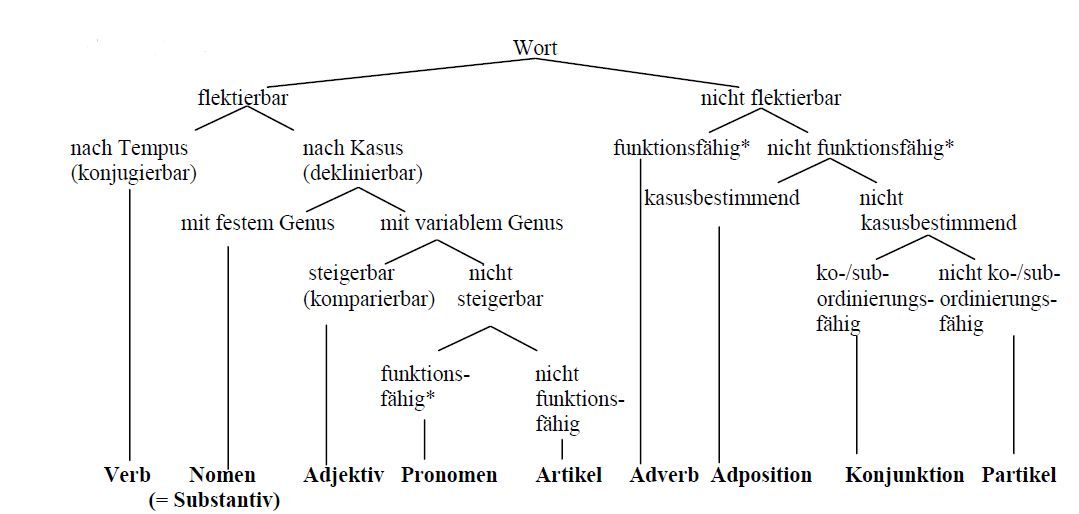
\includegraphics[scale=.4]{material/07wortartenklassifikation}

	
\scalebox{.55}{\begin{forest}MyP edges,
		[Wort
			[flektierbar
				[{nach Tempus\\(konjugierbar)}
				[\textbf{Verb}]
				]
				[{nach Kasus \\(deklinierbar)}
					[{mit festem \\ Genus}
					[{\textbf{Nomen}\\ (\textbf{Substantiv})}]
					]
					[{mit variablem \\Genus}
						[{steigerbar \\(komparierbar)} [\textbf{Adjektiv}] ]
						[{nicht \\steigerbar}
							[funktionsfähig [\textbf{Pronomen}] ]
							[{nicht \\ funktionsfähig} [\textbf{Artikel}] ]
						]
					]
				]
			]
			[{nicht \\flektierbar}
				[funktionsfähig [\textbf{Adverb}] ]
				[{nicht \\funktionsfähig }
					[kasusbestimmend [\textbf{Adposition}] ]
					[{nicht \\kasusbestimmend}
						[{ko-/ \\subordinierungs-\\fähig} [\textbf{Konjunktion}] ]
						[{nicht ko-/ \\ subordinierungs-\\fähig} [\textbf{Partikel}] ]
					]
				]
			]
		]
	\end{forest}}
	\caption{Wortartenklassifikation \citep{Repp&Co15a}}
\end{figure}

\end{frame}


%%%%%%%%%%%%%%%%%%%%%%%%%%%%%%%%%%
\begin{frame}
\frametitle{Wortarten}
\begin{itemize}
	\item \textbf{Schwierigkeiten} mit prototypischen Eigenschaften:

	\eal 
	\ex mithilfe 
	\ex mit Hilfe
	\zl
	
\pause 
Präposition oder Präposition $+$ Nomen ($+$ Nomen im Genitiv?)
\pause

	\ea bausparen 
	\z

\pause	
	nicht V2-fähig wie die \gqq{gewöhnlichen} Verben

\end{itemize}

\end{frame}

%%%%%%%%%%%%%%%%%%%%%%%%%%%%%%%%%%%%%%%

\begin{frame}
\frametitle{Wortarten}

	\begin{itemize}
			\item \textbf{Schwierigkeiten} mit prototypischen Eigenschaften:
				\ea Das \textbf{Schlafen}
			\z
			
			\pause
			Verb oder Nomen?
				\eal
			\ex Er \textbf{kauft} Brot. 
			\ex Er hat das Brot \textbf{gekauft}.
			\pause
			\ex Das \textbf{gekaufte} Brot
			\zl
			
			\pause
			Verb oder Adjektiv?
	\end{itemize}
\end{frame}


%%%%%%%%%%%%%%%%%%%%%%%%%%%%%%%%%%
\begin{frame}
\frametitle{Wortarten}

\begin{itemize}

	\item In unserem Kurs:

\end{itemize}

\begin{table}
\centering
\scalebox{0.9}{
\begin{tabular}{lll}
\textbf{Wortart} & \textbf{Abk.} & \textbf{Beispiel} \\ 
\hline
Nomen (Substantiv) & N & Tisch, Liebe, Maria \\ 
\hline
Determinierer (Artikel, Quantor, Pronomen) & D & der, dem, alle, ein, ich \\ 
\hline
Adjektiv & A & schön, syntaktisch \\ 
\hline
Adverb & Adv & heute, hier \\ 
\hline
Verb & V & rennen, malen \\ 
\hline
Adposition (Prä- \& Postposition) & P & vor, in, wegen, entlang \\ 
\hline
Komplementierer (Subjunktion) & C & ob, dass, weil \\ 
\hline
Konjunktion & K & und, aber, sondern \\ 
\hline
Partikel & Part & ja, wohl, leider \\ 
\hline
\end{tabular} 
}

\end{table}

\end{frame}


%%%%%%%%%%%%%%%%%%%%%%%%%%%%%%%%%%
%%%%%%%%%%%%%%%%%%%%%%%%%%%%%%%%%%
\subsection{Konstituenten}

\iftoggle{sectoc}{
	\frame{
%		\begin{multicols}{2}
		\frametitle{~}
		\tableofcontents[currentsubsection,subsubsectionstyle=hide]
%		\end{multicols}
	}
}


%%%%%%%%%%%%%%%%%%%%%%%%%%%%%%%%%%
\begin{frame}
\frametitle{Konstituenten}

\begin{itemize}
	\item Nicht nur Wörter, sondern auch größere Einheiten spielen in der Syntax eines Satzes eine wichtige Rolle.
	\item Pausen beim Vorlesen:
	\ea Eine 16 Jahre alte Französin starb nach dem Verzehr eines Döners an Lebensmittelvergiftung.\jambox{(Quelle: \url{www.frauenzimmer.de})}
	\z
	
\pause	
	\item Verschiebungen in einem Satz:
	\eal 
	\ex[]{Eine 16 Jahre alte Französin starb \alertred{[nach dem Verzehr]} eines Döners an Lebensmittelvergiftung.}
	\ex[]{\alertred{[Nach dem Verzehr eines Döners]} starb eine 16 Jahre alte Französin an Lebensmittelvergiftung.}
	\ex[*]{\alertred{[Nach dem Verzehr]} starb eine 16 Jahre alte Französin \alertred{[eines Döners]} an Lebensmittelvergiftung.}
	\zl


\end{itemize}

\end{frame}


%%%%%%%%%%%%%%%%%%%%%%%%%%%%%%%%%%
\begin{frame}
\frametitle{Konstituenten}

\begin{itemize}
	\item Wörter bilden (\textbf{konstituieren}) mit anderen Wörtern Konstituenten, die dann gemeinsam größere Konstituenten bilden (vgl.\ Morphologie).
	
	\eal
	\ex{\alertgreen{eines} $+$ [Döners] \pause $=$ \alertred{[eines Döners]}}
	
\pause	
	
	\ex{\alertgreen{Verzehr} $+$ [eines Döners] $=$ \alertred{[Verzehr eines Döners]}}
\pause
	
	\ex{\alertgreen{dem} $+$ [Verzehr eines Döners] $=$ \alertred{[dem Verzehr eines Döners]}}
\pause
	
	\ex{\alertgreen{nach} $+$ [dem Verzehr eines Döners] $=$ \alertred{[nach dem Verzehr eines Döners]}}
	\zl

\end{itemize}

\end{frame}


%%%%%%%%%%%%%%%%%%%%%%%%%%%%%%%%%%
\begin{frame}

\begin{itemize}
	\item Die Gehirnaktivität verdeutlicht die hierarchische Struktur des Satzes (s.\ \citealt{Devitt15a} (pro Chomsky) \vs \citealt{Boutonnet15a} (contra Chomsky)).	
\end{itemize}

\begin{figure}
\centering
%	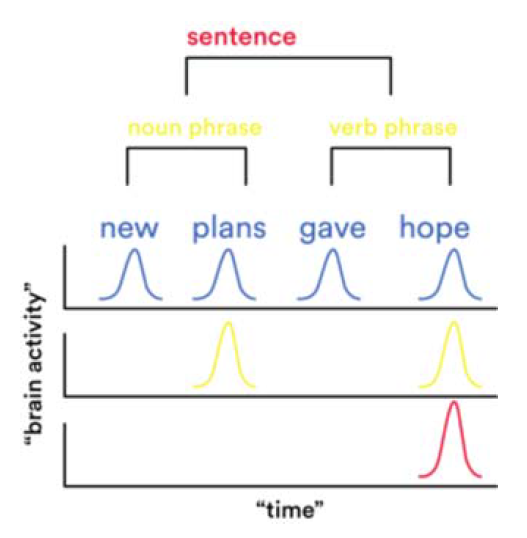
\includegraphics[scale=.33]{material/10gehirnaktivitaet}
	
\begin{tikzpicture}[scale=.48]
	\draw[black](9,0)--(0,0)--(0,1.5);
	\draw[black](9,2)--(0,2)--(0,3.5);
	\draw[black](9,4)--(0,4)--(0,5.5);
	\draw[black](1.5,6.5)--(1.5,7)--(3.5,7)--(3.5,6.5);
	\draw[black](6,6.5)--(6,7)--(8,7)--(8,6.5);
	\draw[black](2.5,8)--(2.5,8.5)--(7,8.5)--(7,8);	
	\node[rotate=90,right] (brain activity) at (-0.6,0) {\scriptsize Gehirnaktivität};
	\node[right] (time) at (2.5,-0.6) {\scriptsize Zeit};
	\node[above] (sentence) at (4.25,8.3) {\scriptsize \alertred{sentence}};
	\node[below] (noun) at (2.5,8) {\scriptsize \alertgreen{noun phrase}};
	\node[below] (verb) at (7,8) {\scriptsize \alertgreen{verbal phrase}};
	\node[below] (new) at (1.5,6.4) {\scriptsize \alertblue{new}};
	\node[below] (plans) at (3.5,6.5) {\scriptsize \alertblue{plans}};
	\node[below] (gave) at (6,6.4) {\scriptsize \alertblue{gave}};
	\node[below] (hope) at (8,6.5) {\scriptsize \alertblue{hope}};	
	\draw[HUblue] (0.75,4.4) sin (1,4.3) cos (1.25,5) sin (1.5,5.5) cos (1.75,5) sin (2,4.3) cos (2.25, 4.4);
	\draw[HUblue] (2.75,4.4) sin (3,4.3) cos (3.25,5) sin (3.5,5.5) cos (3.75,5) sin (4,4.3) cos (4.25, 4.4);
	\draw[HUblue] (5.25,4.4) sin (5.5,4.3) cos (5.75,5) sin (6,5.5) cos (6.25,5) sin (6.5,4.3) cos (6.75, 4.4);
	\draw[HUblue] (7.25,4.4) sin (7.5,4.3) cos (7.75,5) sin (8,5.5) cos (8.25,5) sin (8.5,4.3) cos (8.75,4.4);
	\draw[HUgreen] (7.25,2.4) sin (7.5,2.3) cos (7.75,3) sin (8,3.5) cos (8.25,3) sin (8.5,2.3) cos (8.75,2.4);
	\draw[HUgreen] (2.75,2.4) sin (3,2.3) cos (3.25,3) sin (3.5,3.5) cos (3.75,3) sin (4,2.3) cos (4.25, 2.4);
	\draw[HUred] (7.25,0.4) sin (7.5,0.3) cos (7.75,1) sin (8,1.5) cos (8.25,1) sin (8.5,0.3) cos (8.75,0.4);
\end{tikzpicture}
\caption{\citep[Nach:][]{Boutonnet15a}}
\end{figure}

\end{frame}


%%%%%%%%%%%%%%%%%%%%%%%%%%%%%%%%%%%
\begin{frame}
\frametitle{Konstituenten}

\begin{itemize}
	\item Konstituente: relational zu anderen Konstituenten und zum dem, was sie konstituieren (\ras einfach vs. komplex)
	\medskip
	\item Bei den Konstituenten ist es wichtig herauszufinden, welche sich in Sätzen wie eine \textbf{strukturelle Einheit} verhalten.
	\medskip
	\item In der traditionellen Grammatik \ras Satzglieder und Satzgliedteile

\end{itemize}

\end{frame}


%%%%%%%%%%%%%%%%%%%%%%%%%%%%%%%%%%%
\begin{frame}
\frametitle{Konstituenten}

\begin{itemize}

	\item \textbf{Konstituententests} \citep[vgl.][]{MyP18a}
	\begin{itemize}
		\item Ersetzungstest (oder Substitutionstest)
		\item Pronominalisierungstest
		\item Fragetest
		\item Verschiebetest (oder Permutationstest)
		\item Vorfeldtest (oder Voranstellungstest) 
		\item Weglasstest (oder Eliminierungstest)
		\item (Koordinationstest, Parenthesetest, \dots )
	\end{itemize}
	\medskip
	\item (Phrasale) Konstituenten sollten sich \textbf{in den meisten} dieser Tests \textbf{als syntaktische Einheit verhalten}.

\end{itemize}

\end{frame}


%%%%%%%%%%%%%%%%%%%%%%%%%%%%%%%%%%%
%%%%%%%%%%%%%%%%%%%%%%%%%%%%%%%%%%
\subsubsection{Ersetzungstest}

%\iftoggle{sectoc}{
%	\frame{
%		\begin{multicols}{2}
%		\frametitle{~}
%		\tableofcontents[currentsubsection,subsubsectionstyle=hide]
%		\end{multicols}
%	}
%}

%%%%%%%%%%%%%%%%%%%%%%%%%%%%%%%%%%%
\begin{frame}
\frametitle{Ersetzungstest (Substitutionstest)}

\begin{itemize}
	\item Was sich durch ein anderes Wort (/""eine andere Wortfolge) ersetzen lässt, so dass der Satz grammatisch bleibt, ist (vermutlich) eine (phrasale) Konstituente.

	\eal 
	\ex[]{\alertred{[Eine Frau]} starb nach dem Verzehr eines Döners.}
	\ex[]{\alertred{[Ein Mann]} starb nach dem Verzehr eines Döners.}
	\ex[*]{\alertred{[Ein Mann]} nach dem Verzehr eines Döners.}
	\zl

\pause	
	\eal 
	\ex Die Frau hat versucht, \alertred{[den Döner zu genießen]}.
	\ex Die Frau hat versucht, \alertred{[uns allen Weihnachtsgeschenke zu geben]}.
	\zl
	
\end{itemize}

\nocite{MyP18m}

\end{frame}


%%%%%%%%%%%%%%%%%%%%%%%%%%%%%%%%%%%
%%%%%%%%%%%%%%%%%%%%%%%%%%%%%%%%%%
\subsubsection{Pronominalisierungstest}

%\iftoggle{sectoc}{
%	\frame{
%		\begin{multicols}{2}
%		\frametitle{~}
%		\tableofcontents[currentsubsection,subsubsectionstyle=hide]
%		\end{multicols}
%	}
%}

%%%%%%%%%%%%%%%%%%%%%%%%%%%%%%%%%%%
\begin{frame}
\frametitle{Pronominalisierungstest}

\begin{itemize}
	\item Unterart des Ersetzungstests
	\medskip
	\item Was sich durch ein Pronomen ersetzen lässt, so dass der Satz grammatisch bleibt, ist (vermutlich) eine (phrasale) Konstituente.

	\eal 
	\ex[]{\alertred{[Eine Frau]} starb \alertred{[nach dem Verzehr eines Döners]}.}
	\ex[]{\alertred{[Sie]} starb \alertred{[dann]}.}
	\ex[*]{\alertred{[Sie]} nach dem Verzehr eines Döners.}
	\ex[*]{Eine Frau \alertred{[dann]}.}
	\zl

\pause	
	\eal 
	\ex Die Frau versucht, \alertred{[den Döner zu genießen]}.
	\ex Die Frau versucht \alertred{[das]}.
	\zl
	
\end{itemize}

\end{frame}


%%%%%%%%%%%%%%%%%%%%%%%%%%%%%%%%%%%
%%%%%%%%%%%%%%%%%%%%%%%%%%%%%%%%%%
\subsubsection{Fragetest}

%\iftoggle{sectoc}{
%	\frame{
%		\begin{multicols}{2}
%		\frametitle{~}
%		\tableofcontents[currentsubsection,subsubsectionstyle=hide]
%		\end{multicols}
%	}
%}

%%%%%%%%%%%%%%%%%%%%%%%%%%%%%%%%%%%
\begin{frame}
\frametitle{Fragetest}

\begin{itemize}
	\item Unterart des Ersetzungstests
	\medskip
	\item Was sich erfragen lässt (durch ein W-Wort ersetzen lässt), so dass der Satz grammatisch bleibt, ist (vermutlich) eine (phrasale) Konstituente.

	\eal 
	\ex[]{\alertred{[Eine Frau]} starb \alertred{[nach dem Verzehr eines Döners]}.}
	\ex[]{\alertred{[Wer]} starb nach dem Verzehr eines Döners?}
	\ex[]{\alertred{[Wann]} starb eine Frau?}
	\ex[*]{\alertred{[Wer]} nach dem Verzehr eines Döners?}
	\ex[*]{\alertred{[Wann]} eine Frau?}
	\zl

\pause	
	\eal 
	\ex Die Frau versucht, \alertred{[den Döner zu genießen]}.
	\ex \alertred{[Was]} versucht die Frau?
	\zl
	
\end{itemize}

\nocite{MyP18j}

\end{frame}


%%%%%%%%%%%%%%%%%%%%%%%%%%%%%%%%%%%
%%%%%%%%%%%%%%%%%%%%%%%%%%%%%%%%%%
\subsubsection{Verschiebetest}


%\iftoggle{sectoc}{
%	\frame{
%		\begin{multicols}{2}
%		\frametitle{~}
%		\tableofcontents[currentsubsection,subsubsectionstyle=hide]
%		\end{multicols}
%	}
%}

%%%%%%%%%%%%%%%%%%%%%%%%%%%%%%%%%%%
\begin{frame}
\frametitle{Verschiebetest (Permutationstest)}

\begin{itemize}
	\item Was sich innerhalb des Satzes verschieben lässt, so dass der Satz grammatisch bleibt, ist (vermutlich) eine (phrasale) Konstituente.

	\eal 
	\ex[]{Nach dem Verzehr eines Döners starb \alertred{[gestern]} \alertred{[eine Frau]}.}
	\ex[]{Nach dem Verzehr eines Döners starb \alertred{[eine Frau]} \alertred{[gestern]}.}
	\ex[*]{Nach dem Verzehr eines Döners starb \alertred{[eine]} [gestern] [Frau].}
	\zl

\pause	
	\eal 
	\ex Die Frau hat noch nicht versucht, \alertred{[den Döner zu genießen]}.
	\ex Die Frau hat \alertred{[den Döner zu genießen]} noch nicht versucht.
	\ex Die Frau hat noch nicht \alertred{[den Döner zu genießen]} versucht.
	\zl

\end{itemize}

\nocite{MyP18l}

\end{frame}


%%%%%%%%%%%%%%%%%%%%%%%%%%%%%%%%%%%
%%%%%%%%%%%%%%%%%%%%%%%%%%%%%%%%%%
\subsubsection{Vorfeldtest}

%\iftoggle{sectoc}{
%	\frame{
%		\begin{multicols}{2}
%		\frametitle{~}
%		\tableofcontents[currentsubsection,subsubsectionstyle=hide]
%		\end{multicols}
%	}
%}


%%%%%%%%%%%%%%%%%%%%%%%%%%%%%%%%%%%
\begin{frame}
\frametitle{Vorfeldtest (Voranstellungstest)}

\begin{itemize}
	\item Unterart des Verschiebetests
	\medskip
	\item Im Deutschen kann vor dem finiten Verb nur eine Konstituente stehen. 
	\medskip
	\item Was sich in einem Aussagesatz vor das finite Verb verschieben lässt, so dass der Satz grammatisch bleibt, ist (vermutlich) eine (phrasale) Konstituente.

\end{itemize}

\end{frame}


%%%%%%%%%%%%%%%%%%%%%%%%%%%%%%%%%%%
\begin{frame}
\frametitle{Vorfeldtest (Voranstellungstest)}

\begin{itemize}
	\item Was sich in einem Aussagesatz vor das finite Verb verschieben lässt, so dass der Satz grammatisch bleibt, ist (vermutlich) eine (phrasale) Konstituente.

	\eal
	\ex[]{\alertred{[Nach dem Verzehr eines Döners]} starb [gestern] [eine Frau].}
	\ex[]{\alertred{[Gestern]} starb [eine Frau] [nach dem Verzehr eines Döners].}
	\ex[]{\alertred{[Eine Frau]} starb [gestern] [nach dem Verzehr eines Döners].}
	\ex[*]{\alertred{[Nach]} starb [eine Frau] [gestern] \alertred{[dem Verzehr eines Döners]}.}
	\ex[*]{\alertred{[Eine]} starb \alertred{[Frau]} [gestern] [nach dem Verzehr eines Döners].}
	\ex[*]{\alertred{[Eines Döners]} starb [eine Frau] [gestern] [nach dem Verzehr].}
	\zl

\end{itemize}

\end{frame}


%%%%%%%%%%%%%%%%%%%%%%%%%%%%%%%%%%%
\begin{frame}
\frametitle{Vorfeldtest (Voranstellungstest)}

\begin{itemize}
	\item Was sich in einem Aussagesatz vor das finite Verb verschieben lässt, so dass der Satz grammatisch bleibt, ist (vermutlich) eine (phrasale) Konstituente.

	\eal 
	\ex[]{Die Frau hat noch nicht versucht, \alertred{[den Döner zu genießen]}.}
	\ex[]{\alertred{[Den Döner zu genießen]} hat die Frau noch nicht versucht.}
	\ex[]{\alertred{[Auf den Döner warten]} wollte er nicht mehr.}
	\ex[*]{\alertred{[den Döner]} wollte er nicht mehr auf warten.}
	\zl

\end{itemize}

\end{frame}


%%%%%%%%%%%%%%%%%%%%%%%%%%%%%%%%%%%
%%%%%%%%%%%%%%%%%%%%%%%%%%%%%%%%%%
\subsubsection{Weglasstest}

%\iftoggle{sectoc}{
%	\frame{
%		\begin{multicols}{2}
%		\frametitle{~}
%		\tableofcontents[currentsubsection,subsubsectionstyle=hide]
%		\end{multicols}
%	}
%}

%%%%%%%%%%%%%%%%%%%%%%%%%%%%%%%%%%%
\begin{frame}
\frametitle{Weglasstest (Eliminierungstest)}

\begin{itemize}
	\item Was sich in elliptischen Konstruktionen weglassen lässt, so dass der Satz grammatisch bleibt, ist (vermutlich) eine (phrasale) Konstituente.

	\eal 
	\ex[]{Maria liebt \sout{[Knoblauchsoße]} und Peter hasst \alertred{[Knoblauchsoße]}.}
	\ex[]{Maria chillt \sout{[an einem sonnigen Tag]} und schreibt Lieder \alertred{[an einem sonnigen Tag]}.}
	\ex[*]{Maria chillt \sout{[an einem]} \alertred{sonnigen Tag} und schreibt Lieder \alertred{[an einem sonnigen Tag]}.}
	\zl

\end{itemize}

\nocite{MyP18f}

\end{frame}


%%%%%%%%%%%%%%%%%%%%%%%%%%%%%%%%%%
%%%%%%%%%%%%%%%%%%%%%%%%%%%%%%%%%%
\subsection{Hausaufgabe}
%\frame{
%\frametitle{~}
%	\tableofcontents[currentsection]
%}
%%%%%%%%%%%%%%%%%%%%%%%%%%%%%%%%%%

%%%%%%%%%%%%%%%%%%%%


\begin{frame}
\frametitle{Hausaufgabe}

\begin{itemize}
	\item Geben Sie die Wortart der folgenden Einheiten an:
\end{itemize}

\begin{columns}
\column{.30\textwidth}
	\begin{enumerate}
	\item Maria
	\item Ach!
	\item kauft
	\item den
	\item an
	\item weil
	\item beachten
	\item obwohl
	\end{enumerate}

\column{.50\textwidth}

\end{columns}

\end{frame}


\iftoggle{ha-loesung}{


%%%%%%%%%%%%%%%%%%%%%%%%%%%%%%%%%%

} 
%%%%%%%%%%%%%%%%%%%%



%%%%%%%%%%%%%%%%%%%%%%%%%%%%%%%%%%
\begin{frame}
\frametitle{Hausaufgabe}

\begin{itemize}
	\item Testen Sie mithilfe von mindestens zwei Konstituententests, ob die fettgedruckten Wortfolgen eine oder mehrere Konstituenten sind.
\end{itemize}

	\ea Maria \textbf{stolperte über} den Stein.

	\ex Der Minister wird in \textbf{der nächsten Woche} die Aussage wiederholen.
	
	\ex Die Besucher beobachteten \textbf{in der Werkstatt bemaltes Porzellan}.
	
	\ex Die Besucher beobachteten \textbf{in der Werkstatt} bemaltes Porzellan.
		
	\ex Erika traf die \textbf{Lehrerin mit den roten Schuhen}.
	
	\ex Helmut hat sehr lange \textbf{auf Maria gewartet}.
	
	\ex Helmut hat sehr lange \textbf{auf Maria} gewartet.
	
	\ex \textbf{Maria wird} nach diesem Kurs Syntax lieben.
	\z
	
\end{frame}
	
%%%%%%%%%%%%%%%%%%%%
\iftoggle{ha-loesung}{
	
	%%%%%%%%%%%%%%%%%%%%%%%%%%%%%%%%
%06b Syntax ha-loesung
%%%%%%%%%%%%%%%%%%%%%%%%%%%%%%


\begin{frame}
\frametitle{Hausaufgabe -- Lösung}

\begin{itemize}
	\item Geben Sie die Wortart der folgenden Einheiten an:
\end{itemize}

\begin{columns}
	\column{.30\textwidth}
	\begin{enumerate}
		\item Maria
		\item Ach!
		\item kauft
		\item den
		\item an
		\item weil
		\item beachten
		\item obwohl
	\end{enumerate}
	
	\column{.50\textwidth}

\pause
	
	\begin{enumerate}
		\item[\ras] \alertgreen{Nomen (Substantiv)}
		\item[\ras] \alertgreen{Interjektion}
		\item[\ras] \alertgreen{Verb}
		\item[\ras] \alertgreen{Determinierer}
		\item[\ras] \alertgreen{Präposition}
		\item[\ras] \alertgreen{Complementizer/Subjunktion}
		\item[\ras] \alertgreen{Verb}
		\item[\ras] \alertgreen{Complementizer/Subjunktion}
	\end{enumerate}
\end{columns}

\end{frame}
	
	
	%%%%%%%%%%%%%%%%%%%%%%%%%%%%%%%%%%
	\begin{frame}
	\frametitle{Hausaufgabe -- Lösung}
	
	
	\begin{itemize}
		\item Testen Sie mithilfe von mindestens zwei Konstituententests, ob die fettgedruckten Wortfolgen eine oder mehrere Konstituenten sind.
		
		\vspace{.5cm}
		
		\item[] Maria \textbf{stolperte über} den Stein.
	\end{itemize}
	
	\pause 
	
	\ea Weglasstest \& Fragetest \ras \alertgreen{keine Konstituente}
	\ea[*]{Maria [stolperte über] den Stein und Peter [\sout{stolperte über}] den Ast.}
	\ex[*]{[Was] Maria den Stein?}
	\z 
	\z
	
\end{frame}


%%%%%%%%%%%%%%%%%%%%%%%%%%%%%%%%%%
\begin{frame}
\frametitle{Hausaufgabe -- Lösung}

\begin{itemize}
\item[] Der Minister wird in \textbf{der nächsten Woche} die Aussage wiederholen.
\end{itemize}

\pause 

\ea Ersetzungstest, Koordinationstest, Fragetest, Vorfeldtest \ras \alertgreen{keine Konstituente}

\ea[??]{Der Minister wird in [dieser] die Aussage wiederholen.}
\ex[?]{Der Minister wird in [der nächsten Woche] und [dem nächsten Treffen] die Aussage wiederholen.}
\ex[*]{[Wann] wird der Minister in die Aussage wiederholen?}
\ex[*]{[Der nächsten Woche] wird der Minister in die Aussage wiederholen.}
\z 
\z

\end{frame}


%%%%%%%%%%%%%%%%%%%%%%%%%%%%%%%%%%
\begin{frame}
\frametitle{Hausaufgabe -- Lösung}

\begin{itemize}
\item[] Die Besucher beobachteten \textbf{in der Werkstatt bemaltes Porzellan}.

\item[] Die Besucher beobachteten \textbf{in der Werkstatt} bemaltes Porzellan.
\end{itemize}

\pause 

\ea Vorfeldtest, Pronominalisierungstest \ras \alertgreen{1 Konstituente} 
\ea {[}In der Werkstatt bemaltes Porzellan{]} beobachteten die Besucher.
\ex Die Besucher beobachteten [es].
\z 

\pause 

\ex Verschiebetest, Pronominalisierungstest, Fragetests \ras \alertgreen{2 Konstituenten}
\ea Die Besucher beobachteten [bemaltes Porzellan] [in der Werkstatt]. 
\ex Die Besucher beobachteten [es] [dort].
\ex {[}Was{]} beobachteten die Besucher [in der Werkstatt]?
\ex {[}Wo{]} beobachteten die Besucher [bemaltes Porzellan]?
\z
\z

\end{frame}


%%%%%%%%%%%%%%%%%%%%%%%%%%%%%%%%%%%%%%%%%%%%%%%%%%%%%%%

\begin{frame}
\frametitle{Hausaufgabe -- Lösung}

\begin{itemize}
\item[] Erika traf die \textbf{Lehrerin mit den roten Schuhen}.
\end{itemize}

\pause 

\ea Weglasstest, Vorfeldtest, Fragetest \ras \alertgreen{keine Konstituente}
\ea[*]{Erika traf die und begrüßte die [Lehrerin mit den roten Schuhen].}
\ex[*]{[Lehrerin mit den roten Schuhen] traf Erika die.}
\ex[*]{[Wen] traf Erika die?}
\z 
\z
\end{frame}


%%%%%%%%%%%%%%%%%%%%%%%%%%%%%%%%%%%%%%%%%%%%%%%%%%%%%%%

\begin{frame}
\frametitle{Hausaufgabe -- Lösung}

\begin{itemize}
\item[] Helmut hat sehr lange \textbf{auf Maria gewartet}.

\item[] Helmut hat sehr lange \textbf{auf Maria} gewartet.
\end{itemize}

\pause 

\ea Vorfeldtest, Fragetest, Verschiebetest \ras \alertgreen{1 aber auch 2 Konstituenten}
\ea[]{[Auf Maria gewartet] hat Helmut sehr lange.}
\ex[]{[Was] hat Helmut sehr lange?}
\ex[??]{Helmut hat [auf Maria gewartet] sehr lange.}
\ex[]{Helmut hat [auf Maria] sehr lange [gewartet].}
\ex[]{[Auf Maria] hat Helmut sehr lange gewartet.} 
\z
\z 

\end{frame}


%%%%%%%%%%%%%%%%%%%%%%%%%%%%%%%%%%%%%%%%%%%%%%%%%%%%%%

\begin{frame}
\frametitle{Hausaufgabe -- Lösung}

\begin{itemize}
\item[] \textbf{Maria wird} nach diesem Kurs Syntax lieben.
\end{itemize}

\pause 

\ea Verschiebetest, Fragetest, Weglasstest \ras \alertgreen{keine Konstituente}
\ea[*]{Nach diesem Kurs [Maria wird] Syntax lieben.}
\ex[*]{[Wer] nach diesem Semester Syntax lieben?}
\ex[]{[Maria wird] nach diesem Kurs Syntax lieben und [\sout{Maria wird}] nur noch an Bäume denken.}
\z 
\z

\end{frame}
	
} 
%%%%%%%%%%%%%%%%%%%%


%%%%%%%%%%%%%%%%%%%%%%%%%%%%%%%%%%
\subsection{Sonstiges}
%\frame{
%\frametitle{~}
%	\tableofcontents[currentsection]
%}


%%%%%%%%%%%%%%%%%%%%%%%%%%%%%%%%%%
\begin{frame}
\frametitle{Was Sie sich zu Weihnachten wünschen können\dots}

\begin{itemize}
	\item \citet{Glueck&Roedel16a} (auch über die HU-Bibliothek herunterladbar)
	\item \citet{Luedeling2009a}
	\item \citet{Brandt&Co06a}
	\item \citet{Grewendorf&Co91a}
	\item \citet{Chomsky65a}
	\item \citet{MuellerS15b} (auch über die Webseite herunterladbar)
	\item \citet{MuellerS13f} (auch über die Webseite herunterladbar)
	\item \citet{Pinker95a}

\end{itemize}

\end{frame}


%%%%%%%%%%%%%%%%%%%%%%%%%%%%%%%%%%
\begin{frame}
\frametitle{Frohe Weihnachten!}

\begin{figure}
\centering
\scalebox{.7}{
	\begin{forest}MyP edges,
[TP
	[DP [\zerobar{D} [\textcolor{orange}{\textbf{this}} ] ] ]
	[\MyPxbar{T}
		[\zerobar{T} [\textcolor{violet}{\textbf{is\textsubscript{i}}}] ]
		[VP 
			[\zerobar{V} [\textcolor{blue}{\textbf{t\textsubscript{i}}}] ]
			[DP
				[\zerobar{D} [\textcolor{magenta}{\textbf{my}}] ]
				[NP
				[AP [\zerobar{A} [\textcolor{red}{\textbf{christmas}} ] ] ]
					[\zerobar{N} [\textcolor{green}{\textbf{tree}}] ]
				]
			]
		]
	]
]
\end{forest}
}
\caption{Weihnachtsbaum}
\end{figure}
%\begin{figure}
%\centering
%	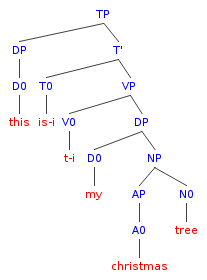
\includegraphics[scale=.57]{material/09xmastree}
%	\caption{Frohe Weihnachten!}
%\end{figure}

\end{frame}

%%%%%%%%%%%%%%%%%%%%%%%%%%%%%%%%%%

\subsection{Abbildungen}
\begin{frame}{Abbildungen}
\small

\begin{itemize}
	\item ABBILDUNG -- \gqq{Noam Chomsky. Aufgenommen von John Soares, 2005} (Stevertigo, Zugriff: 18.07.2018) \url{https://upload.wikimedia.org/wikipedia/commons/8/86/Noam_chomsky.jpg}
	\item ABBILDUNG -- \gqq{Schimpansenfamilie} (Stock-Foto, Zugriff: 18.07.2018) \url{https://www.colourbox.de/bild/familie-auf-der-oberseite-des-baumes-bild-2566359}
\end{itemize}	

\end{frame}

%%%%%%%%%%%%%%%%%%%%%%%%%%%%%%%%%%%%%%%%%%%%%%%%
%% Compile the master file!
%% 		Slides: Antonio Machicao y Priemer
%% 		Course: GK Linguistik
%%%%%%%%%%%%%%%%%%%%%%%%%%%%%%%%%%%%%%%%%%%%%%%%


%%%%%%%%%%%%%%%%%%%%%%%%%%%%%%%%%%%%%%%%%%%%%%%%%%%%
%%%             Metadata                         
%%%%%%%%%%%%%%%%%%%%%%%%%%%%%%%%%%%%%%%%%%%%%%%%%%%%      


\title{Grundkurs Linguistik}

\subtitle{Syntax III: Topologisches Feldermodell, Satztypen \& Satzmodi}

\author[A. Machicao y Priemer]{
	{\small Antonio Machicao y Priemer}
	\\
	{\footnotesize \url{http://www.linguistik.hu-berlin.de/staff/amyp}}\\
%	\href{mailto:mapriema@hu-berlin.de}{mapriema@hu-berlin.de}}
}

\institute{Institut für deutsche Sprache und Linguistik}

%\date{ }

%\publishers{\textbf{6. linguistischer Methodenworkshop \\ Humboldt-Universität zu Berlin}}

%\hyphenation{nobreak}


%%%%%%%%%%%%%%%%%%%%%%%%%%%%%%%%%%%%%%%%%%%%%%%%%%%%
%%%             Preamble's End                  
%%%%%%%%%%%%%%%%%%%%%%%%%%%%%%%%%%%%%%%%%%%%%%%%%%%%      


%%%%%%%%%%%%%%%%%%%%%%%%%      
\huberlintitlepage[22pt]
\iftoggle{toc}{
\frame{
\begin{multicols}{2}
	\frametitle{Inhaltsverzeichnis}\tableofcontents
	%[pausesections]
\end{multicols}
	}
	}


%%%%%%%%%%%%%%%%%%%%%%%%%%%%%%%%%%
%%%%%%%%%%%%%%%%%%%%%%%%%%%%%%%%%%
%%%%%LITERATURE:

%% Allgemein
\nocite{Glueck&Roedel16a}
\nocite{Luedeling2009a} 
\nocite{Meibauer&Co07a} 
\nocite{Repp&Co15a} 

%% Morphologie
%\nocite{Eisenberg04}

%% Syntax
%\nocite{Adger04a}
\nocite{Altmann&Hofmann08a} % Satztypen & Satzmodi
\nocite{Altmann93a} % Satztypen & Satzmodi
\nocite{Brandt&Co06a} 
%\nocite{Fries&MyP16b} % Akzeptabilität
%\nocite{Fries16a} % Grammatikalität
%\nocite{Fries&MyP16d} % Kompetenz vs Performanz
%\nocite{Fries&MyP16c} % GG
%\nocite{Fries&MyP16a} % X-Bar-Theorie
\nocite{Fries16e} % Satztyp
\nocite{Fries16d} % Satzmodus 
\nocite{Grewendorf&Co91a} 
%\nocite{MyP17b} % Kerngrammatik
%\nocite{MyP18a} % Konstituententest
%\nocite{MyP18b} % Kopf
\nocite{MyP18c} % Phrase
%\nocite{MuellerS13f} 
%\nocite{MuellerS15b}
%\nocite{Stechow&Sternefeld88a}
%\nocite{Sternefeld06a}
%\nocite{Sternefeld06b}
\nocite{Woellstein10a} % Topologisches Feldermodell

%%%%%%%%%%%%%%%%%%%%%%%%%%%%%%%%%%

\begin{frame}
	\frametitle{Begleitlektüre}
		\begin{itemize}
			\item \textbf{obligatorisch:}
				\begin{itemize}
					\item[] AM S.~69--79
					\item[] \citet{MyP18c}
				\end{itemize}
		\end{itemize}
\end{frame}


%%%%%%%%%%%%%%%%%%%%%%%%%%%%%%%%%%
\section{Syntax III}
%%%%%%%%%%%%%%%%%%%%%%%%%%%%%%%%%%

\subsection{Das topologische Modell}

\iftoggle{sectoc}{
	\frame{
		%\begin{multicols}{2}
		\frametitle{~}
		\tableofcontents[currentsubsection,subsubsectionstyle=hide]
		%\end{multicols}
	}
}


%%%%%%%%%%%%%%%%%%%%%%%%%%%%%%%%%%
\begin{frame}
\frametitle{Das topologische Modell}

\begin{block}{Topologie (Satztopologie, Feldgliederung)}
Zusammenfassende Bezeichnung für das Studium der Wortstellung und der Satzgliedstellung, d.\,h.\ der Anordnung der entsprechenden Elemente im Raum (Geschriebenes) oder der Zeit (Gesprochenes). \\ \hfill \citep[vgl.][]{Glueck16a, Staffeldt16a}
\end{block}

\pause 

\begin{itemize}

	\item Zweck: Wortstellung im deutschen Matrixsatz abzubilden (\textbf{Topologie})
%	\item[]
	\item Hilfreich für die \textbf{Beschreibung} und den \textbf{Vergleich} von Satzstrukturen
%	\item[]
	\item Es erfasst alle möglichen deutschen Satztypen und macht sie \textbf{vergleichbar}.
%	\item[]
	\item Syntaktische Strukturen können \textbf{topologisch} erfasst werden, d.\,h.\ ihre Elemente werden in ihren Positionen und Abfolgen \textbf{beschrieben}.

\end{itemize}

\end{frame}


%%%%%%%%%%%%%%%%%%%%%%%%%%%%%%%%%%%
\begin{frame}
\frametitle{Das topologische Modell}

\begin{itemize}
	\item Die toplogische Satzstrukturbetrachtung hat eine lange Tradition.
	
	\ras \citealt{Herling1821a-u}; \citealt{Erdmann1886a-Short}; \textbf{\citealt{Drach39a}}
	
	\item[]
	\item Die \textbf{Verfeinerung} des Modells wurde in den 1980ern vorgenommen. 
	
	\ras \citealt{Reis80a-link}; \citealt{Hoehle83a}; \citealt{Hoehle85a} \\
	\hfill \citep[vgl.][]{MRR2018a-ed}
	
	\item[]
	
	\item Topologisches Modell wird (für einige Fragesetllungen) immer noch verwendet.
	
	\ras \citealt{Ramers06a}; \citealt{Pafel09}; \citealt{Woellstein10a} 


\end{itemize}

\end{frame}


%%%%%%%%%%%%%%%%%%%%%%%%%%%%%%%%%%
%%%%%%%%%%%%%%%%%%%%%%%%%%%%%%%%%%
\subsubsection{Dreifeldermodell}

%\iftoggle{sectoc}{
%	\frame{
%		\begin{multicols}{2}
%		\frametitle{~}
%		\tableofcontents[currentsubsection,subsubsectionstyle=hide]
%		\end{multicols}
%	}
%}


%%%%%%%%%%%%%%%%%%%%%%%%%%%%%%%%%%
\begin{frame}
\frametitle{Dreifeldermodell (Drach 1937)}

\begin{itemize}
	\item Drachs Dreifeldermodell war ursprünglich für die Erfassung von \textbf{Aussagesätzen mit Verbzweitstellung} (V2-Sätze) gedacht.
	\item[]
	\item \textbf{Vorfeld (VF):} Abschnitt vor dem finiten Verb
	\item \textbf{Mitte:} Position für das finite Verb
	\item \textbf{Nachfeld (NF):} Abschnitt nach dem finiten Verb
\end{itemize}

\pause

\begin{table}
\centering

\begin{tabular}{l|l|l}
\textbf{Vorfeld} & \textbf{Mitte} & \textbf{Nachfeld} \\ 
\hline 
Sophia & \alertred{schreibt} & ihre Dissertation. \\ 
\hline
\pause
Sophia & \alertred{hat}  & ihre Dissertation geschrieben. \\ 
\hline 
\pause
Ihre Dissertation geschrieben & \alertred{hat} & Sophia längst!\\ 
\end{tabular} 

\end{table}

\end{frame}


%%%%%%%%%%%%%%%%%%%%%%%%%%%%%%%%%%
\begin{frame}
\frametitle{Dreifeldermodell (Drach 1937)}

\begin{itemize}
	\item \textbf{Probleme:}
	
	\begin{itemize}
		\item Modell erfasst nicht den komplexen Bereich nach dem finiten Verb.
		\item[]
		\item Modell nur für V2-Strukturen \ras zu beschränkt		
	\end{itemize}
\end{itemize}

\pause

\eal
\ex \alertred{Hat} [Sophia] [ihre Dissertation] \alertred{geschrieben}?
\ex \alertred{Schreib} endlich deine Diss!
\ex	\alertred{Ob} sie ihre Diss \alertred{schreibt}?
\zl


\end{frame}


%%%%%%%%%%%%%%%%%%%%%%%%%%%%%%%%%%
%%%%%%%%%%%%%%%%%%%%%%%%%%%%%%%%%%
\subsubsection{Uniformes Grundmodell}

%\iftoggle{sectoc}{
%	\frame{
%		\begin{multicols}{2}
%		\frametitle{~}
%		\tableofcontents[currentsubsection,subsubsectionstyle=hide]
%		\end{multicols}
%	}
%}


%%%%%%%%%%%%%%%%%%%%%%%%%%%%%%%%%
\begin{frame}
\frametitle{Uniformes Grundmodell (in unserem Kurs)}

\begin{itemize}
	\item Auch: Stellungsfeldermodell,  lineares Modell, Felderstrukturenmodell 
	\item 5-gliedriges Grundmodell
	\item Erfasst \textbf{mehr Daten} als das Dreifeldermodell (d.\,h. es ist beschreibungsadäquater) 
	
	\ras Alle Verbstellungs- bzw. Satztypen werden in einem \textbf{einheitlichen} Muster abgebildet.
\end{itemize}

\end{frame}

%%%%%%%%%%%%%%%%%%%%%%%%%%%%%%%%%%%%%%%%%%%%
\begin{frame}

\begin{itemize}
	\item Satz in topologische Abschnitte eingeteilt:
	\begin{itemize}
		\item []
		\item \textbf{Vorfeld (VF):} Feld vor dem finiten Verb
		\item[]
		\item \textbf{Linke Satzklammer (LSK):} Finites Verb oder Subjunktion
		\item[]
		\item \textbf{Mittelfeld (MF):} 0--$x$ Konstituente(n)
		\item[]		
		\item \textbf{Rechte Satzklammer (RSK):} Verb(komplex)
		\item[]		
		\item \textbf{Nachfeld (NF):} Satzartige oder \gqq{schwere} Konstituenten
	\end{itemize}
\pause
\end{itemize}

\begin{table}
\centering
\scalebox{0.85}{
\begin{tabular}{l|l|l|l|l}
\textbf{VF} & \textbf{LSK} & \textbf{MF} & \textbf{RSK} & \textbf{NF} \\ 
\hline 
Gestern & ist & Nathalie früh nach Hause & gegangen, & weil sie müde war. \\ 
\end{tabular} 
}
\end{table}
	
 \end{frame}


%%%%%%%%%%%%%%%%%%%%%%%%%%%%%%%%%%
\begin{frame}

\begin{itemize}
	\item Abschnitte bzw.\ Satzeinheiten resultieren aus der Stellung der finiten und/""oder infiniten Verbform ($\approx$ aus dem Verbkomplex).
\end{itemize}

\begin{table}
\centering
\scalebox{0.8}{
\begin{tabular}{l|l|l|l|l}
\textbf{VF} & \textbf{LSK} & \textbf{MF} & \textbf{RSK} & \textbf{NF} \\ 
\hline 
Nathalie & \alertred{ist} & zu Hause & \alertred{geblieben}, & weil sie krank ist. \\ 
\end{tabular} 
}
\end{table}

\end{frame}


%%%%%%%%%%%%%%%%%%%%%%%%%%%%%%%%%%
\begin{frame}

\begin{itemize}
	\item Analyse von \textbf{Haupt- und Nebensätzen} und \textbf{komplexen Satzstrukturen} möglich!
	\item[]
	\item Dieses Modell erfasst die \textbf{Verbklammer} (typisch für das Deutsche) und
	die \textbf{Komplementarität} zwischen \textbf{Verb und Complementizer} in der LSK.
\end{itemize}

\begin{table}
\centering
\scalebox{0.8}{
\begin{tabular}{l|l|l|l|l}
\textbf{VF} & \textbf{LSK} & \textbf{MF} & \textbf{RSK} & \textbf{NF} \\ 
\hline 
Nathalie & \alertred{ist} & zu Hause & \alertgreen{geblieben}, & weil sie krank ist. \\ 
\hline
$\emptyset$ & \alertred{weil} & sie krank & \alertgreen{ist} & $\emptyset$. \\ 
\end{tabular} 
}
\end{table}

\end{frame}


%%%%%%%%%%%%%%%%%%%%%%%%%%%%%%%%%%%
%%%%%%%%%%%%%%%%%%%%%%%%%%%%%%%%%%
\subsubsection{Eigenschaften der Felder}

%\iftoggle{sectoc}{
%	\frame{
%		\begin{multicols}{2}
%		\frametitle{~}
%		\tableofcontents[currentsubsection,subsubsectionstyle=hide]
%		\end{multicols}
%	}
%}


%%%%%%%%%%%%%%%%%%%%%%%%%%%%%%%%%%
\begin{frame}
\frametitle{Eigenschaften der Felder}

\begin{itemize}
	\item \textbf{VF:}

\begin{table}
\centering
\scalebox{0.8}{
\begin{tabular}{l|l|l|l|l}
\textbf{VF} & \textbf{LSK} & \textbf{MF} & \textbf{RSK} & \textbf{NF} \\ 
\hline 
\alertred{Marlijn} & ist & zu Hause. &  &  \\
\hline 
\alertred{Die Frau, die hier arbeitet,} & ist & sehr fleißig. & & \\  
\alertred{obwohl die Heizung ausgeschaltet ist,} & & & & \\
\hline
\alertred{$\emptyset$} & ist & Marlijn zu Hause ? &  &  \\
\hline
\alertred{$\emptyset$} & weil & sie krank & ist. &  \\ 
\end{tabular} 
}

\end{table}

\pause

\begin{itemize}
	\item \textbf{Fakultativ} besetzt
	\item Platz für \textbf{eine} (beliebig komplexe) Konstituente 
	\item \textbf{Leer} bei 
	
	\begin{itemize}
		\item sog. V1-Sätzen (Entscheidungsfragen, Imperativsätzen, \dots ),
		
		\item Sätzen mit nebensatzeinleitender Konjunktion ($\approx$ Complementizer): \MyPobj{dass}, \MyPobj{ob}, \MyPobj{weil}, \dots 
	
	\end{itemize}	
\end{itemize}


\end{itemize}

\end{frame}


%%%%%%%%%%%%%%%%%%%%%%%%%%%%%%%%%%
\begin{frame}
\frametitle{Eigenschaften der Felder}

\begin{itemize}
	\item \textbf{LSK:}

\begin{table}
\centering
\scalebox{0.8}{
\begin{tabular}{l|l|l|l|l|l}
& \textbf{VF} & \textbf{LSK} & \textbf{MF} & \textbf{RSK} & \textbf{NF} \\ 
\hline 
& Petra & \alertred{macht} & einen guten Kaffee. &  &  \\
\hline 
& & \alertred{dass} & Petra einen guten Kaffee & macht & \\  
\hline
Ich weiß, & wer & \alertred{$\emptyset$} & sie & ist. &  \\
\hline
Die Dame, & die & \alertred{$\emptyset$} & hier & arbeitet &  \\ 
\end{tabular} 
}
\end{table}

\pause 

\begin{itemize}
	\item Entweder finites Verb oder Complementizer
	\item \textbf{Leer} bei 
	
	\begin{itemize}
		\item eingebetteten Konstituentenfragen, 
		\item Relativsätzen, 
		\item Infinitivsätzen, \dots
	\end{itemize}
\end{itemize}

\end{itemize}

	
\end{frame}


%%%%%%%%%%%%%%%%%%%%%%%%%%%%%%%%%%
\begin{frame}
\frametitle{Eigenschaften der Felder}

\begin{itemize}
	\item \textbf{MF:}

\begin{table}
\centering
\scalebox{0.75}{
\begin{tabular}{l|l|l|l|l}
\textbf{VF} & \textbf{LSK} & \textbf{MF} & \textbf{RSK} & \textbf{NF} \\ 
\hline 
Sophie & hat & \alertred{gut} & geschlafen. & \\  
\hline 
Sophie & soll & \alertred{[trotz des Bahnchaos']} & bekommen haben. &  \\
& & \alertred{[nach ihrem Gespräch]} &  &  \\
& & \alertred{[in einer anderen Stadt]} &  &  \\
& & \alertred{[einen guten Job]} &  &  \\
\hline 
Sophie & hat & \alertred{$\emptyset$} & geschlafen. & \\  
\hline
Sie & hat & \alertred{die Frau} & eingestellt, & \alertred{die am qualifiziertesten} \\
 &  &  & & \alertred{war}. \\
\end{tabular} 
}
\end{table}

\pause 

\begin{itemize}
	\item Platz für \textbf{beliebig viele} Konstituenten
	\item Fakultativ auch leer
	\item Durch RSK können Konstituenten des MFs aufgebrochen werden.
\end{itemize}


\end{itemize}

\end{frame}


%%%%%%%%%%%%%%%%%%%%%%%%%%%%%%%%%%
\begin{frame}
\frametitle{Eigenschaften der Felder}

\begin{itemize}
	\item \textbf{RSK:}

\begin{table}
\centering
\scalebox{0.8}{
\begin{tabular}{l|l|l|l|l}
\textbf{VF} & \textbf{LSK} & \textbf{MF} & \textbf{RSK} & \textbf{NF} \\ 
\hline 
Monika & mag &  & \alertred{unterrichten}. & \\  
\hline 
 & Ob & Monika & \alertred{unterrichtet}? &  \\
\hline
mit dem & & Monika zur Arbeit & \alertred{fährt} &  \\
\hline
& weil & Monika & \alertred{angerufen haben will} &  \\
\hline
Monika & hat &  & \alertred{angerufen}. &  \\
\hline 
Monika & ruft &  & \alertred{an}.&  \\
\end{tabular} 
}
\end{table}

\pause 

\begin{itemize}
	\item Infinite Verben 
	\item Finites Verb (falls nicht in LSK) \ras \zB in Neben- oder Relativsätzen
	\item Fakultativ auch leer
\end{itemize}

\end{itemize}

\end{frame}


%%%%%%%%%%%%%%%%%%%%%%%%%%%%%%%%%%
\begin{frame}
\frametitle{Eigenschaften der Felder}

\begin{itemize}
	\item \textbf{NF:}

\begin{table}
\centering
\scalebox{0.8}{
\begin{tabular}{l|l|l|l|l}
\textbf{VF} & \textbf{LSK} & \textbf{MF} & \textbf{RSK} & \textbf{NF} \\ 
\hline 
Maria & hat &  & gesehen, & \alertred{dass Peter schläft}.\\  
\hline 
Maria & hat &  & gesehen, & \alertred{als sie in die Küche kam}\\  
 &  &  & & \alertgreen{dass Peter schlief}.\\  
\hline
Sie & hat & \alertred{die Frau} & eingestellt, & \alertred{die am qualifiziertesten} \\
 &  &  & & \alertred{war}. \\
\hline
Du & hast & uns alle & begeistert & \alertred{mit deiner großartigen Präsentation}. \\
\end{tabular} 
}
\end{table}

\pause 

\begin{itemize}
	\item Kann eine oder mehrere Konstituenten enthalten
	\item Fakultativ leer
	\item Hauptsächlich besetzt bei Subjekt-, Objekt-, Adverbial- oder Relativsätzen (Extraposition)
	\item Fakultativ auch bei \gqq{schweren} Konstituenten (PPs)
\end{itemize}


\end{itemize}

\end{frame}


%%%%%%%%%%%%%%%%%%%%%%%%%%%%%%%%%%
\begin{frame}

\begin{itemize}
	\item Im VF, MF, NF kann ein Satz enthalten sein (oder mehrere), der selbst wieder nach dem Feldermodell analysiert werden kann. 


\begin{table}
\centering
\scalebox{0.8}{
\begin{tabular}{l|l|l|l|l}
\textbf{VF} & \textbf{LSK} & \textbf{MF} & \textbf{RSK} & \textbf{NF} \\ 
\hline 
Maria & hat &  & gesehen, & \alertred{dass Peter schläft}.\\
\hline
 & dass & Peter & schläft & \\  
\hline
\hline 
Maria & hat &  & gemerkt, & \alertred{dass Peter denkt},\\  
 &  &  & & \alertred{dass sie schläft}.\\ 
\hline
   & dass & Peter & denkt, & \alertgreen{dass sie schläft}\\ 
\hline
   & dass & sie & schläft &  \\ 
\hline   
\hline
\alertred{Dass Peter denkt,} & hat & Maria sehr schnell & gemerkt. & \\
\alertgreen{dass sie schläft,} &  &  & & \\
\hline
\hline
Maria & hat, & \alertred{obwohl sie geschlafen hat}, & erwischt. &  \\
& & die Einbrecher & & \\
\end{tabular} 
}
\end{table}

\end{itemize}

\end{frame}


%%%%%%%%%%%%%%%%%%%%%%%%%%%%%%%%%%%
%%%%%%%%%%%%%%%%%%%%%%%%%%%%%%%%%%
\subsubsection{Fazit}

%\iftoggle{sectoc}{
%	\frame{
%		\begin{multicols}{2}
%		\frametitle{~}
%		\tableofcontents[currentsubsection,subsubsectionstyle=hide]
%		\end{multicols}
%	}
%}

%%%%%%%%%%%%%%%%%%%%%%%%%%%%%%%%%%
\begin{frame}
\frametitle{Fazit}

\begin{itemize}
	\item Das topologische Feldermodell eröffnet Möglichkeiten zur \textbf{Beschreibung} von \textbf{strukturellen (linearen) Gesetzmäßigkeiten} im Satzbau (\zB Satzklammer) und von grammatischen Konzepten (\zB Satztyp).
	\item[]
	\item Für eine intensive Beschäftigung mit der deutschen Syntax ist das Uniforme Modell allein allerdings \textbf{nicht ausreichend}. Die Unterteilung ist zu grob. Es sind Erweiterungen nötig. 
	
	vgl. Dreifeldermodell \ras Uniformes Modell \ras Differenzmodell
	\\ \hfill \citep[vgl.][]{Woellstein10a}

\end{itemize}

\end{frame}

%%%%%%%%%%%%%%%%%%%%%%%%%%%%%%%%%%
%%%%%%%%%%%%%%%%%%%%%%%%%%%%%%%%%%
\subsubsection{Übung}

%\iftoggle{sectoc}{
%	\frame{
%		\begin{multicols}{2}
%		\frametitle{~}
%		\tableofcontents[currentsubsection,subsubsectionstyle=hide]
%		\end{multicols}
%	}
%}


%%%%%%%%%%%%%%%%%%%%%%%%%%%%%%%%%%

%\iftoggle{uebung}{

\begin{frame}
\frametitle{Übung}

\begin{itemize}
	\item[1.] Ordnen Sie die folgenden \textbf{Matrixsätze} in das topologische Modell ein:


\eal
\ex Christiane schläft.
\ex Schläft Christiane?
\ex Ob Christiane schläft?
\ex Schlaf!
\ex Dass Christiane schläft, ist mir klar.
\ex Ich wusste, dass Christiane schläft.
\ex Er hat sich gedacht, dass Christiane wieder schläft.
%\ex Weil wir es uns nicht vorstellen konnten, haben wir uns gewundert, dass Christiane schläft.
\ex Weil wir es uns nicht vorstellen konnten, haben wir uns gewundert, als wir gemerkt haben, dass Christiane schläft.
\zl

\end{itemize}

\end{frame}

%}
%%%%%%%%%%%%%%%%%%%%%%%%%%%%%%

\iftoggle{ue-loesung}{

%%%%%%%%%%%%%%%%%%%%%%%%%%%%%%%%%%%%%%%%%%%%%%%%%%%
%06c Syntax ue-loesung01
%%%%%%%%%%%%%%%%%%%%%%%%%%%%%%%%%%%%%%%%%%%%%
	
\begin{frame}
\frametitle{Übung -- Lösung}

\begin{table}
\centering
\scalebox{0.75}{
\begin{tabular}{p{3.5cm}|p{1cm}|p{2.5cm}|p{1.5cm}|p{3.5cm}}
\textbf{VF} & \textbf{LSK} & \textbf{MF} & \textbf{RSK} & \textbf{NF} \\ 
\hline 
\alertgreen{Christiane} & \alertgreen{schläft.} & & & \\
\hline
& \alertgreen{Schläft} & \alertgreen{Christiane?} & & \\
\hline
& \alertgreen{Ob} & \alertgreen{Christiane} & \alertgreen{schläft?} & \\
\hline
& \alertgreen{Schlaf!} & & & \\
\hline
\alertgreen{Dass Christiane schläft,} & \alertgreen{ist} & \alertgreen{mir klar.} & & \\
\hline
\alertgreen{Ich} & \alertgreen{wusste,} & \alertgreen{dass Christiane schläft.} & & \\
\hline
\alertgreen{Er} & \alertgreen{hat} & \alertgreen{sich} & \alertgreen{gedacht,} & \alertgreen{dass Christiane wieder schläft.} \\
\hline
%\alertgreen{Weil wir es uns nicht vorstellen konnten,} & \alertgreen{haben} & \alertgreen{wir uns} & \alertgreen{gewundert,} & \alertgreen{dass Christiane schläft.} \\
%\hline
\alertgreen{Weil wir es uns nicht vorstellen konnten,} & \alertgreen{haben} & \alertgreen{wir uns} & \alertgreen{gewundert,} & \alertgreen{als wir gemerkt haben, dass Christiane schläft.} \\
\end{tabular}
}
\end{table}

\end{frame}

}

%%%%%%%%%%%%%%%%%%%%%%%%%%%%%%%%%%

%\iftoggle{uebung}{

\begin{frame}
\frametitle{Übung}

\begin{itemize}

	\item[2.] Ordnen Sie die folgenden \textbf{Sätze und ihre eingebetteten Nebensätze} in das topologische Modell ein:
\eal
\ex Dass Christiane schläft, ist mir klar.
\ex Ich wusste, dass Christiane schläft.
\ex Er hat sich gedacht, dass Christiane wieder schläft.
\ex Weil wir es uns nicht vorstellen konnten, haben wir uns gewundert, dass Christiane schläft.
\ex Weil wir es uns nicht vorstellen konnten, haben wir uns gewundert, als wir gemerkt haben, dass Christiane schläft.
\ex Die Frau, die die roten Schuhe trägt, schläft wieder.
%\ex Als Sophia in der Flüchtlingsunterkunft geholfen hat, hat sie dort den jungen Mann getroffen, mit dem sie sich ein Büro teilt.  	
\zl
	
\end{itemize}

\end{frame}

%}
%%%%%%%%%%%%%%%%%%%%%%%%%%%%%%%%%
\iftoggle{ue-loesung}{

%%%%%%%%%%%%%%%%%%%%%%%%%
%06c ue-loesung02
%%%%%%%%%%%%%%%%%%%%%%%%%

\begin{frame}
\frametitle{Übung -- Lösung}

\begin{table}
\centering
\scalebox{0.63}{
\begin{tabular}{p{5cm}|p{1cm}|p{4cm}|p{1.5cm}|p{4cm}}
\textbf{VF} & \textbf{LSK} & \textbf{MF} & \textbf{RSK} & \textbf{NF} \\ 
\hline
\alertgreen{Dass Christiane schläft,} & \alertgreen{ist} & \alertgreen{mir klar.} & & \\
\hline
& \alertgreen{Dass} & \alertgreen{Christiane} & \alertgreen{schläft} & \\
\hline
\alertgreen{Ich} & \alertgreen{wusste,} & \alertgreen{dass Christiane schläft.} & & \\
\hline
& \alertgreen{dass} & \alertgreen{Christiane} & \alertgreen{schläft.} & \\
\hline
\alertgreen{Er} & \alertgreen{hat} & \alertgreen{sich} & \alertgreen{gedacht,} & \alertgreen{dass Christiane wieder schläft.} \\
\hline
& \alertgreen{dass} & \alertgreen{Christiane wieder} & \alertgreen{schläft.} & \\
\hline
\alertgreen{Weil wir es uns nicht vorstellen konnten,} & \alertgreen{haben} & \alertgreen{wir uns} & \alertgreen{gewundert,} & \alertgreen{dass Christiane schläft.}\\
\hline
& \alertgreen{Weil} & \alertgreen{wir es uns nicht} & \alertgreen{vorstellen konnten} & \\
\hline
& \alertgreen{dass} & \alertgreen{Christiane} & \alertgreen{schläft.} & \\
\hline
\alertgreen{Die Frau, die die roten Schuhe trägt,} & \alertgreen{schläft} & \alertgreen{wieder.} & & \\
\hline
\alertgreen{Die Frau, die} & & \alertgreen{die roten Schuhe} & \alertgreen{trägt} & \\
%\hline
%\alertgreen{Als Sophia in der Flüchtlingsunterkunft geholfen hat,} & \alertgreen{hat} & \alertgreen{sie dort den jungen Mann} & \alertgreen{getroffen,} & \alertgreen{mit dem sie sich ein Büro teilt.} \\
%\hline
%& \alertgreen{Als} & \alertgreen{Sophia in der Flüchtlingsunterkunft} & \alertgreen{geholfen hat} & \\
%\hline
%\alertgreen{mit dem} & & \alertgreen{sie sich ein Büro} & \alertgreen{teilt.} & \\
\end{tabular}
}
\end{table}

\end{frame}



}

%%%%%%%%%%%%%%%%%%%%%%%%%%%%%%%%%%

\subsection{Satztypen \& Satzmodi}

\iftoggle{sectoc}{
	\frame{
%		\begin{multicols}{2}
		\frametitle{~}
		\tableofcontents[currentsubsection,subsubsectionstyle=hide]
%		\end{multicols}
	}
}


%%%%%%%%%%%%%%%%%%%%%%%%%%%%%%%%%%
\begin{frame}
\frametitle{Satztypen \& Satzmodi}

\begin{itemize}
	\item Sätze im Deutschen können verschiedene \textbf{Formen} annehmen:
	\begin{itemize}
		\item \textbf{Verberststellung (V1)}
		\eal 
		\ex \label{ex:Frage} \alertred{Schläft} Norbert?
		\ex \label{ex:Imperat} \alertred{Schlaf} endlich!
		\zl
		
		\item \textbf{Verbzweitstellung (V2)}
		\ea \label{ex:Dekl} Norbert \alertred{schläft} gerne nach dem Mittagessen.
		\z
		
		\item \textbf{Verbletztstellung (VL)}
		\ea \label{ObFrage} Ob Norbert \alertred{schnarcht}?
		\z
		
	\end{itemize}	

\pause

	\item Verschiedene Formen entsprechen unterschiedlichen \textbf{Funktionen:}
	\begin{itemize}
		\item etwas in der Welt als \textbf{wahr} zu postulieren (\ref{ex:Dekl}),
		\item Zweifel oder \textbf{Unwissen} auszudrücken (\ref{ex:Frage}), (\ref{ObFrage}),
		\item etwas auszudrücken, von dem man \textbf{will, dass es wahr ist} (/wird) (\ref{ex:Imperat}).		
	\end{itemize}
\end{itemize}

\end{frame}


%%%%%%%%%%%%%%%%%%%%%%%%%%%%%%%%%%
\begin{frame}
\frametitle{Satztypen \& Satzmodi}

\begin{block}{Satzmodus}
Klassifikation von komplexen Zeichen (Sätzen) \textbf{mit einer Form- und einer Funktionsseite}. Der Sprecher wählt also eine bestimmte Form aus, um eine bestimmte Funktion zu erfüllen \citep[vgl.][]{Altmann93a}.
\end{block}


\pause 


\begin{block}{Satztyp}
Bezeichnung für unterschiedliche \textbf{Formtypen} von Sätzen, insbesondere solcher Hauptsätze, die in Äußerungen divergierende Handlungszwecke erfüllen bzw.\ erfüllen können \citep[vgl.][]{Fries16d, Fries16e}.
\end{block}


\end{frame}


%%%%%%%%%%%%%%%%%%%%%%%%%%%%%%%%%%
\begin{frame}
\frametitle{Satztypen \& Satzmodi}

\begin{itemize}
	\item \textbf{Formtyp} (Satztyp) \ras Formseite
	\begin{itemize}
		\item morphologische, syntaktische, phonologische Merkmale
		\item satzförmige Struktur mit formellen Eigenschaften
		\item Wort-/Verbstellung
		\item Verbmorphologie
		\item Subkategorisierung
		\item Kategoriale Füllung
		\item Intonation, \dots
	\end{itemize}

	\item \textbf{Funktionstyp} \ras Funktionsseite
	\begin{itemize}
		\item Bedeutung zum Ausdruck einer Proposition oder zur Ausführung einer sprachlichen Handlung vom spezifischen Satztyp: etwas assertieren/""erfragen/""befehlen/""wünschen \dots\ 
	\end{itemize}
\end{itemize}

\end{frame}


%%%%%%%%%%%%%%%%%%%%%%%%%%%%%%%%%%
\begin{frame}
\frametitle{Satztypen \& Satzmodi}

Die wichtigsten Satzmodi des Deutschen ausgehend von (\ref{ex:TypModus}):

\ea\label{ex:TypModus} Proposition: \gqq{Uta ihr Auto verschenkt}
\z

\pause 

\begin{itemize}
	\item \textbf{Modus}: Deklarativ(-satz); Aussage(satz) 
	
	prototyp. \textbf{Satztyp}: Deklarativsatz
	\ea Uta verschenkt ihr Auto.
	\z

\pause 
	
	\item \textbf{Modus}: Interrogativ(-satz); Frage(satz)
	
	prototyp. \textbf{Satztyp}: Interrogativsatz
	
	\ea Verschenkt Uta ihr Auto?
	\ex Ob Uta ihr Auto verschenkt?
	\z
\end{itemize}

\end{frame}


%%%%%%%%%%%%%%%%%%%%%%%%%%%%%%%%%%
\begin{frame}
\frametitle{Satztypen \& Satzmodi}


\begin{itemize}
	\item \textbf{Modus}: Imperativ(-satz); Aufforderungs(satz) 
	
	prototyp. \textbf{Satztyp}: Imperativsatz
	\ea Verschenk dein Auto, Uta!
	\z

\pause 
	
	\item \textbf{Modus}: Exklamativ(-satz); Ausrufe(satz)
	
	prototyp. \textbf{Satztyp}: ?
	
	\ea Uta hat ihr Auto verschenkt!
	\z

\pause 
	
	\item \textbf{Modus}: Optativ(-satz); Wunsch(satz)
	
	prototyp. \textbf{Satztyp}: ?
	
	\ea Wenn Uta nur ihr Auto verschenken würde!
	\z
	
\end{itemize}

Exklamativ und Optativ gelten wegen \textbf{des fehlenden eigenen Satztypen im Deutschen} als marginal.


\end{frame}


%%%%%%%%%%%%%%%%%%%%%%%%%%%%%%%%%%
%%%%%%%%%%%%%%%%%%%%%%%%%%%%%%%%%%
\subsubsection{Deklarativ}

%\iftoggle{sectoc}{
%	\frame{
%		\begin{multicols}{2}
%		\frametitle{~}
%		\tableofcontents[currentsubsection,subsubsectionstyle=hide]
%		\end{multicols}
%	}
%}


%%%%%%%%%%%%%%%%%%%%%%%%%%%%%%%%%%
\begin{frame}
\frametitle{Deklarativ}

\begin{itemize}
	\item \textbf{Satztyp:} V2-Aussagesatz
	\begin{itemize}
		\item Subkategorisierung: Kein W-Fragewort
		\item Verbstellung: V2 (V in LSK)
		\item Verbmodus: Indikativ (oder Konjunktiv)
		\item Intonation: fallend
	\end{itemize}
	\item \textbf{Funktionstyp:}
	\begin{itemize}
		\item unmarkierter Satzmodus
		\item kann für unterschiedliche Sprechakte verwendet werden (Behauptung, Mitteilung, Vermutung, Aufforderung, \dots )
	\end{itemize}
	
	\ea Du machst heute deine Hausaufgaben.
	\z
	
\end{itemize}

\end{frame}


%%%%%%%%%%%%%%%%%%%%%%%%%%%%%%%%%%
%%%%%%%%%%%%%%%%%%%%%%%%%%%%%%%%%%
\subsubsection{Interrogativ: E-Interrogativ}

%\iftoggle{sectoc}{
%	\frame{
%		\begin{multicols}{2}
%		\frametitle{~}
%		\tableofcontents[currentsubsection,subsubsectionstyle=hide]
%		\end{multicols}
%	}
%}


%%%%%%%%%%%%%%%%%%%%%%%%%%%%%%%%%%
\begin{frame}
\frametitle{Interrogativ: E-Interrogativ}

\begin{itemize}
	\item Auch: Entscheidungsfrage(satz)
	\item \textbf{Satztyp:} V1-Fragesatz $|$ VL-Fragesatz $+$ \MyPobj{ob}
	\begin{itemize}
		\item Subkategorisierung: Kein W-Fragewort $|$ \MyPobj{ob} in LSK
		\item Verbstellung: V1 (V in LSK), VF leer $|$  VL (V in RSK)
		\item Verbmodus: Indikativ (oder Konjunktiv)
		\item Intonation: steigend
	\end{itemize}
	\item \textbf{Funktionstyp:}
	\begin{itemize}
		\item relativ unmarkierter Satzmodus
		\item kann für unterschiedliche Sprechakte verwendet werden: Fragen, Bitten, Aufforderung, \dots
		\item Eine Antwort wird verlangt.
	\end{itemize}
	
	\eal
	\ex Machst du heute deine Hausaufgaben?
	\ex Ob du heute deine Hausaufgaben machst?
	\zl
	
\end{itemize}

\end{frame}


%%%%%%%%%%%%%%%%%%%%%%%%%%%%%%%%%%
%%%%%%%%%%%%%%%%%%%%%%%%%%%%%%%%%%
\subsubsection{Interrogativ: K-Interrogativ}

%\iftoggle{sectoc}{
%	\frame{
%		\begin{multicols}{2}
%		\frametitle{~}
%		\tableofcontents[currentsubsection,subsubsectionstyle=hide]
%		\end{multicols}
%	}
%}

%%%%%%%%%%%%%%%%%%%%%%%%%%%%%%%%%%
\begin{frame}
\frametitle{Interrogativ: K-Interrogativ}

\begin{itemize}
	\item Auch: Konstituentenfrage(satz)
	\item \textbf{Satztyp:} V2-Fragesatz
	\begin{itemize}
		\item Subkategorisierung: W-Fragewort im VF
		\item Verbstellung: V2 (V in LSK)
		\item Verbmodus: Indikativ (oder Konjunktiv)
		\item Intonation: steigend
	\end{itemize}
	\item \textbf{Funktionstyp:}
	\begin{itemize}
		\item Eine Antwort wird dem Fragewort entsprechend verlangt.
	\end{itemize}
	
	\eal
	\ex Was machst du heute?
	\ex Wer macht heute seine Hausaufgaben?
	\zl
	
\end{itemize}

\nocite{MyP18e} \nocite{MyP18g} \nocite{MyP18i} \nocite{MyP18p}

\end{frame}


%%%%%%%%%%%%%%%%%%%%%%%%%%%%%%%%%%
%%%%%%%%%%%%%%%%%%%%%%%%%%%%%%%%%%
\subsubsection{Imperativ}

%\iftoggle{sectoc}{
%	\frame{
%		\begin{multicols}{2}
%		\frametitle{~}
%		\tableofcontents[currentsubsection,subsubsectionstyle=hide]
%		\end{multicols}
%	}
%}


%%%%%%%%%%%%%%%%%%%%%%%%%%%%%%%%%%
\begin{frame}
\frametitle{Imperativ}

\begin{itemize}
	\item \textbf{Satztyp:} V1-Imperativsatz (auch V2 möglich)
	\begin{itemize}
		\item Subkategorisierung: kein W-Fragewort, Subjekt in \textsc{2.sg} und \textsc{pl} wird getilgt
		\item Verbstellung: V1 oder V2 (V in LSK)
		\item Verbmodus: Imperativ
		\item Intonation: fallend
	\end{itemize}
	\item \textbf{Funktionstyp:}
	\begin{itemize}
		\item zum Ausdrücken von Aufforderungen, Bitten, Befehlen, Drohungen, \dots
	\end{itemize}
	
	\eal
	\ex Mach heute deine Hausaufgaben!
	\ex Machen Sie heute Ihre Hausaufgaben!
	\ex Jetzt macht doch eure Hausaufgaben!
	\zl
	
\end{itemize}

\end{frame}


%%%%%%%%%%%%%%%%%%%%%%%%%%%%%%%%%%
%%%%%%%%%%%%%%%%%%%%%%%%%%%%%%%%%%
\subsubsection{Exklamativ}

%\iftoggle{sectoc}{
%	\frame{
%		\begin{multicols}{2}
%		\frametitle{~}
%		\tableofcontents[currentsubsection,subsubsectionstyle=hide]
%		\end{multicols}
%	}
%}


%%%%%%%%%%%%%%%%%%%%%%%%%%%%%%%%%%
\begin{frame}
\frametitle{Exklamativ}

\begin{itemize}
	\item \textbf{Satztyp:} V1-Exklamativsatz (auch V2 möglich)
	\begin{itemize}
		\item Subkategorisierung: keine Negation, kann W-Wort enthalten, häufig Verwendung von Partikeln
		\item Verbstellung: V1, V2 oder VL
		\item Verbmodus: eher Indikativ
		\item Intonation: fallend
	\end{itemize}
	\item \textbf{Funktionstyp:}
	\begin{itemize}
		\item zum Ausdrücken von Überraschungen (nicht dialogisch!)
	\end{itemize}
	
	\eal
	\ex Hat er (aber auch) tolle Hausaufgaben abgegeben!
	\ex Er hat (aber auch) tolle Hausaufgaben abgegeben!
	\ex Was für tolle Hausaufgaben er abgegeben hat!
	\ex Was für tolle Hausaufgaben hat er abgegeben!
	\zl
		
\end{itemize}

\end{frame}


%%%%%%%%%%%%%%%%%%%%%%%%%%%%%%%%%%
%%%%%%%%%%%%%%%%%%%%%%%%%%%%%%%%%%
\subsubsection{Optativ}

%\iftoggle{sectoc}{
%	\frame{
%		\begin{multicols}{2}
%		\frametitle{~}
%		\tableofcontents[currentsubsection,subsubsectionstyle=hide]
%		\end{multicols}
%	}
%}


%%%%%%%%%%%%%%%%%%%%%%%%%%%%%%%%%%
\begin{frame}
\frametitle{Optativ}

\begin{itemize}
	\item \textbf{Satztyp:} V1-Optativsatz $|$ VL $+$ \MyPobj{wenn}
	\begin{itemize}
		\item Subkategorisierung: kein W-Fragewort, häufig Verwendung von \MyPobj{nur} oder \MyPobj{doch} $|$ \MyPobj{wenn} $+$ VL
		\item Verbstellung: V1 $|$ VL
		\item Verbmodus: Konjunktiv
		\item Intonation: fallend
	\end{itemize}
	\item \textbf{Funktionstyp:}
	\begin{itemize}
		\item zum Ausdrücken von irrealen Wünschen (nicht dialogisch!)
	\end{itemize}
	
	\eal
	\ex Hätte er (doch/""nur) tolle Hausaufgaben abgegeben! 
	\ex Wenn er (doch/""nur) tolle Hausaufgaben abgegeben hätte!
	\zl
		
\end{itemize}

\end{frame}


%%%%%%%%%%%%%%%%%%%%%%%%%%%%%%%%%%
%%%%%%%%%%%%%%%%%%%%%%%%%%%%%%%%%%
\subsection{Hausaufgabe}
%\frame{
%\frametitle{~}
%	\tableofcontents[currentsection]
%}
%%%%%%%%%%%%%%%%%%%%%%%%%%%%%%%%%%


\begin{frame}
\frametitle{Hausaufgabe}

\begin{itemize}
	\item Bestimmen Sie den Satzmodus der folgenden Sätze, geben Sie dabei die Merkmale zur Bestimmung des Satztyps, sowie den möglichen Funktionstyp an. 
\end{itemize}


\ea \label{ex:Rechnung} Wir haben unsere Rechnungen bezahlt. 
%\ex \label{ex:krank} Ob ich morgen noch krank bin? 
%\ex \label{ex:Wagen} Er hätte einen Wagen kaufen können. 
\ex \label{ex:Folien} Hast du endlich die Folien fertig?
\ex \label{ex:Iss} Iss!
\ex \label{ex:Geld} Wenn ich nur Geld hätte!
%\ex \label{ex:spät} Kannst du mir sagen, wie spät es ist?
%\ex \label{ex:Störung} Verzeihen Sie die Störung.
\ex \label{ex:geschlagen} Wen hast du geschlagen?
\ex \label{ex:gewonnen} Ich habe gewonnen!
%\ex \label{ex:Prüfung} Wenn ich doch die Prüfung bestehe, kaufe ich mir ein Auto.
%\ex \label{ex:Baum} Was für einen tollen Baum hat er gemalt? 
%\ex \label{ex:leise} Sie sind jetzt aber leise!
%\ex \label{ex:Verständnis} Wir bitten um Verständnis.
\z

\end{frame}


%%%%%%%%%%%%%%%%%%%%%%%%%%%%%%%%%%
	
\begin{frame}
\frametitle{Hausaufgabe}

\begin{itemize}
	\item Geben Sie eine Analyse der folgenden Sätze (\textbf{inkl. Nebensätze}) nach dem topologischen Feldermodell.
\end{itemize}

	\ea \label{ex:Top1} Wenn ich die Prüfung bestehe, werde ich mir ein Buch von Chomsky kaufen.
	\ex \label{ex:Top2} Werde ich mir das Buch kaufen, wenn ich bestehe?
	\z 		
	
\end{frame}

%%%%%%%%%%%%%%%%%%%%%%%%%%%%%%%%%%%	

\iftoggle{ha-loesung}{
	
	%%%%%%%%%%%%%%%%%%
%06c Syntax ha-loesung
%%%%%%%%%%%%%%%%%%

\begin{frame}
\frametitle{Hausaufgabe -- Lösung}

\begin{itemize}
	\item Bestimmen Sie den Satzmodus der folgenden Sätze, geben Sie dabei die Merkmale zur Bestimmung des Satztyps, sowie den möglichen Funktionstyp an. 
\end{itemize}

\begin{exe}
\exr{ex:Rechnung} Wir haben unsere Rechnungen bezahlt.

\pause 
	\begin{itemize}
		\item \alertgreen{Satzmodus: Deklarativsatz}
		\item \alertgreen{Satztyp: V2"=Aussagesatz (Kein W"=Fragewort, Indikativ, Intonation: fallend)}
		\item \alertgreen{Funktionstyp: unmarkierte Mitteilung}
	\end{itemize}
%
%\exr{ex:krank} Ob ich morgen noch krank bin? 
%
%\alertred{E-Interogativsatz (VL + ob), Frage, Antwort wird verlangt}
%
%\ex \label{ex:Wagen} Er hätte einen Wagen kaufen können. 
%	
%	\alertred{Deklarativsatz (V2), unmarkierte Vermutung}
%
\exr{ex:Folien} Hast du endlich die Folien fertig?

\pause	
\begin{itemize}
		\item \alertgreen{Satzmodus: E-Interrogativsatz}
		\item \alertgreen{Satztyp: V1"=Fragesatz (Kein Fragewort, Indikativ, Intonation: steigend)}
		\item \alertgreen{Funktionstyp: auffordernde Frage (\ras Beeil dich!), Antwort wird verlangt}
\end{itemize}

\end{exe}

\end{frame}


%%%%%%%%%%%%%%%%%%%%%%%%%%%%%%%%%%%%%%%
\begin{frame}
\frametitle{Hausaufgabe -- Lösung} 

\begin{exe}

\exr{ex:Iss} Iss!

\pause
\begin{itemize}
	\item \alertgreen{Satzmodus: Imperativsatz}
	\item \alertgreen{Satztyp: V1"=Imperativsatz (kein W"=Fragewort, Tilgung des Subjekts in 2.Sg., V1, Verbmodus: Imperativ, fallende Intonation)}
	\item \alertgreen{Funktionstyp: Aufforderung/Befehl}
\end{itemize}

\exr{ex:Geld} Wenn ich nur Geld hätte!

\pause
\begin{itemize}
	\item \alertgreen{Satzmodus: Optativ}
	\item \alertgreen{Satztyp: VL + wenn, kein W"=Fragewort, Verwendung von \emph{nur}, Konjunktiv, fallende Intonation}
	\item \alertgreen{Funktionstyp: irrealer Wunsch}
\end{itemize}
%
%\exr{ex:spät} Kannst du mir sagen, wie spät es ist? 
%
%\alertred{E-Interrogativ (V1) + K-Interrogativ (VL), wenn die erste Teilantwort \gqq{ja} ist, dann folgt eine Antwort auf das Fragewort (\gqq{Ja, es ist \dots\ Uhr.})}
%
%\ea \label{ex:Störung} Verzeihen Sie die Störung.
%
%\alertred{Imperativ (V1), Bitte}
%
\end{exe} 

\end{frame}


%%%%%%%%%%%%%%%%%%%%%%%%%%%%%%%%%%%%%%%
\begin{frame}
\frametitle{Hausaufgabe -- Lösung} 

\begin{exe}
	
\exr{ex:geschlagen} Wen hast du geschlagen?

\pause 
\begin{itemize}
	\item \alertgreen{Satzmodus: K"=Interrogativ}
	\item \alertgreen{Satztyp: V2"=Fragesatz, W"=Fragewort im VF, Indikativ, steigende Intonation}
	\item \alertgreen{Funktionstyp: Antwort auf Fragewort wird verlangt}
\end{itemize}


\exr{ex:gewonnen} Ich habe gewonnen!

\pause
\begin{itemize}
	\item \alertgreen{Satzmodus: Exklamativ}
	\item \alertgreen{Satztyp: V2, keine Negation, Indikativ, fallende Intonation}
	\item \alertgreen{Funktionstyp: Ausdruck einer Überraschung}
\end{itemize}
%
%\exr{ex:Prüfung} Wenn ich doch die Prüfung bestehe, kaufe ich mir ein Auto.
%
%\alertred{Deklarativ (V2), an Bedingung geknüpfte Mitteilung}
%
%\exr{ex:Baum} Was für einen tollen Baum hat er gemalt? 
%
%\alertred{K-Interrogativ, Verständnis-Nachfrage}
%
%\exr{ex:leise} Sie sind jetzt aber leise!
%
%\alertred{Imperativ (V2), Befehl/ Aufforderung}
%
%\exr{ex:Verständnis} Wir bitten um Verständnis.
%
%\alertred{Deklarativ (V2), Aufforderung}
%
\end{exe}

\end{frame}


%%%%%%%%%%%%%%%%%%%%%%%%%%%%%%%%%%%%%%%
\begin{frame}
	\frametitle{Hausaufgabe -- Lösung} 
	
\begin{itemize}
	\item Geben Sie eine Analyse der folgenden Sätze (\textbf{inkl. Nebensätze}) nach dem topologischen Feldermodell.
\end{itemize}
	
\begin{exe}
	\exr{ex:Top1} Wenn ich die Prüfung bestehe, werde ich mir ein Buch von Chomsky kaufen.
	\exr{ex:Top2} Werde ich mir das Buch kaufen, wenn ich bestehe?
\end{exe}
	
	
	
\begin{table}
	\centering
	\scalebox{0.8}{
		\alertgreen{\begin{tabular}{p{3.5cm}|l|p{4cm}|p{1.5cm}|p{3cm}}
				\textbf{VF} & \textbf{LSK} & \textbf{MF} & \textbf{RSK} & \textbf{NF} \\ 
				\hline
				Wenn ich die Prüfung bestehe, & werde & ich mir ein Buch von Chomsky & kaufen. &\\
				\hline
				&Wenn& ich die Prüfung 							& bestehe & \\
				\hline
				\hline 
				&Werde& ich mir das Buch						&kaufen,	& wenn ich bestehe? \\
				\hline 
				&wenn& ich												&bestehe	&\\
		\end{tabular}}
	}
\end{table}
	
	
\end{frame}
}

%%%%%%%%%%%%%%%%%%%%%%%%%%%%%%%%%%%		

%%%%%%%%%%%%%%%%%%%%%%%%%%%%%%%%%%%%%%%%%%%%%%%%
%% Compile the master file!
%% 		Slides: Antonio Machicao y Priemer
%% 		Course: GK Linguistik
%%%%%%%%%%%%%%%%%%%%%%%%%%%%%%%%%%%%%%%%%%%%%%%%


%%%%%%%%%%%%%%%%%%%%%%%%%%%%%%%%%%%%%%%%%%%%%%%%%%%%
%%%             Metadata                         
%%%%%%%%%%%%%%%%%%%%%%%%%%%%%%%%%%%%%%%%%%%%%%%%%%%%      

\title{Grundkurs Linguistik}

\subtitle{Syntax IV: X-Bar-Theorie -- Köpfe}

\author[A. Machicao y Priemer]{
	{\small Antonio Machicao y Priemer}
	\\
	{\footnotesize \url{http://www.linguistik.hu-berlin.de/staff/amyp}}\\
%	\href{mailto:mapriema@hu-berlin.de}{mapriema@hu-berlin.de}}
}

\institute{Institut für deutsche Sprache und Linguistik}

%\date{ }
%\publishers{\textbf{6. linguistischer Methodenworkshop \\ Humboldt-Universität zu Berlin}}


%%%%%%%%%%%%%%%%%%%%%%%%%%%%%%%%%%%%%%%%%%%%%%%%%%%%
%%%             Preamble's End                   %%%
%%%%%%%%%%%%%%%%%%%%%%%%%%%%%%%%%%%%%%%%%%%%%%%%%%%%      


%%%%%%%%%%%%%%%%%%%%%%%%%      
\huberlintitlepage[22pt]
\iftoggle{toc}{
\frame{
\begin{multicols}{2}
	\frametitle{Inhaltsverzeichnis}\tableofcontents
	%[pausesections]
\end{multicols}
	}
	}


%%%%%%%%%%%%%%%%%%%%%%%%%%%%%%%%%%
%%%%%%%%%%%%%%%%%%%%%%%%%%%%%%%%%%
%%%%%LITERATURE:

%% Allgemein
\nocite{Glueck&Roedel16a}
\nocite{Luedeling2009a}
%\nocite{Meibauer&Co07a} 
\nocite{Repp&Co15a} 

%% Morphologie
%\nocite{Eisenberg04}

%% Syntax
\nocite{Adger04a}
%\nocite{Altmann&Hofmann08a} % Satztypen & Satzmodi
%\nocite{Altmann93a} % Satztypen & Satzmodi
\nocite{Brandt&Co06a} 
%\nocite{Fries&MyP16b} % Akzeptabilität
%\nocite{Fries16a} % Grammatikalität
%\nocite{Fries&MyP16d} % Kompetenz vs Performanz
\nocite{Fries&MyP16c} % GG
\nocite{Fries&MyP16a} % X-Bar-Theorie
%\nocite{Fries16e} % Satztyp
%\nocite{Fries16d} % Satzmodus 
\nocite{Grewendorf&Co91a} 
\nocite{Luedeling2009a} 
%\nocite{Meibauer&Co07a}
%\nocite{MyP17b} % Kerngrammatik
\nocite{MyP18a} % Konstituententest
\nocite{MyP18b} % Kopf
\nocite{MyP18c} % Phrase
\nocite{MyP18s} % Funktionale Kategorie
\nocite{MyP18t} % Argumentstruktur
\nocite{MyP18f} %Eliminierungstest
\nocite{MyP18j} %Frageprobe
\nocite{MyP18l} %Permutationstest
\nocite{MyP18m} %Substitutionstest
\nocite{MuellerS13f} 
\nocite{MuellerS15b}
%\nocite{Stechow&Sternefeld88a}
\nocite{Sternefeld06a}
\nocite{Sternefeld06b}
%\nocite{Woellstein10a} % Topologisches Feldermodell
%%%%%%%%%%%%%%%%%%%%%%%%%%%%%%%%%%

\begin{frame}
\frametitle{Begleitlektüre}
	\begin{itemize}
		\item \textbf{obligatorisch:}
			\begin{itemize}
				\item[] AM S.~79--86
			\end{itemize}
	\end{itemize}	
\end{frame}

%%%%%%%%%%%%%%%%%%%%%%%%%%%%%%%%%%
\section{Syntax IV}

%%%%%%%%%%%%%%%%%%%%%%%%%%%%%%%%%%
\subsection{Einleitung}

\iftoggle{sectoc}{
	\frame{
		%\begin{multicols}{2}
		\frametitle{~}
		\tableofcontents[currentsubsection,subsubsectionstyle=hide]
		%\end{multicols}
	}
}

%%%%%%%%%%%%%%%%%%%%%%%%%%%%%%%%%%
\begin{frame}
\frametitle{Einleitung}

\begin{itemize}
	\item Topologisches Modell: nur grobe Gliederung des Satzes in 5 Felder
	\item[]	
	\item feingliedrigere Modellierung: X-Bar-Schema; X-Bar-Modell
	\item[]
	\item Nicht nur für Satzpositionen, sondern auch für Relationen zwischen syntaktischen Einheiten innerhalb von Konstituenten


\eal 
\ex[]{Peter hat gestern \alertred{[den Wagen]} gekauft.}
\ex[]{\alertred{[Den Wagen]} hat Peter gestern gekauft.}
\ex[]{\alertred{[Den Wagen gekauft]} hat Peter gestern.} \label{ex:KonstSatz}
\ex[*]{\alertred{[Den]} hat Peter gestern \alertred{[Wagen]} gekauft.}
\zl

	\item Konstituenten sind nicht immer mit Satzglied gleichzusetzen, vgl.\ (\ref{ex:KonstSatz})
	
\end{itemize}

\end{frame}


%%%%%%%%%%%%%%%%%%%%%%%%%%%%%%%%%%
\begin{frame}
%\frametitle{Einleitung}

\begin{itemize}

	\item \textbf{Intuitiv} können wir sagen, dass (\ref{ex:Klammer1}) grammatisch und (\ref{ex:Klammer2}) ungrammatisch ist.
	\item[]
	\eal
	\ex \label{ex:Klammer1}Klammerstruktur: [$_{VP}$ [$_{NP}$ [$_{Det}$Das] [$_{NP}$Brot]][$_{V}$gekauft]]
	\ex \label{ex:Klammer2}Klammerstruktur: [$_{??}$ [$_{Det}$Das] [$_{??}$ [$_{NP}$Brot][$_{V}$gekauft]]]
	\zl

\end{itemize}


\begin{figure}[b]
	\begin{minipage}[b]{0.05\textwidth}
	\end{minipage} 
	%
	\begin{minipage}[b]{0.40\textwidth}
	\centering
	\scriptsize{
		\begin{forest}
		MyP edges,
		[Das Brot gekauft [Das Brot [Das] [Brot]][gekauft]]
		\end{forest}
		}
		\caption{Baumstruktur (\ref{ex:Klammer1})}	
  	\end{minipage}  
  	%  
	\begin{minipage}[b]{0.05\textwidth}
  	\end{minipage}
  	%         
  	\begin{minipage}[b]{0.40\textwidth}
	\centering
	\scriptsize{
		\begin{forest}
		MyP edges,
		[*Das Brot gekauft [Das][Brot gekauft [Brot] [gekauft]]]
		\end{forest}
		}
		\caption{Baumstruktur (\ref{ex:Klammer2})}
  	\end{minipage}  
  	%              
	\begin{minipage}[b]{0.05\textwidth}
  	\end{minipage}
  	
\end{figure}

\begin{itemize}
	\item Syntax befasst sich \textbf{nicht nur mit der internen Struktur von Sätzen}, sondern \textbf{auch von Phrasen} (manchmal auch von Wörtern)
\end{itemize}
\end{frame}


%%%%%%%%%%%%%%%%%%%%%%%%%%%%%%%%%%
\begin{frame}

\begin{itemize}

	\item \textbf{X-Bar-Theorie}: Sub-Theorie der Generativen Grammatik (GG) seit den 1970er Jahren \citep{Chomsky70a, Jackendoff77x}
	\item[]	
	\item \textbf{GG:} Theoretische Richtung seit den 1950er Jahren \citep{Chomsky57x} (contra Strukturalismus)
	\item[]
\end{itemize}

\begin{columns}
	
\begin{column}{.5\textwidth}

\textbf{Strukturalismus:}
\begin{itemize}
	\item Empirismus (Behaviourismus)
	\item statische Theorie
	\item Beschreibungsadäquat: \textbf{Beschreibung} der in der Sprache vorkommenden Strukturen
\end{itemize}

\end{column}	
%%
%%
\begin{column}{.5\textwidth}

\textbf{GG:}
\begin{itemize}
	\item Rationalismus (UG)
	\item dynamische (generative) Theorie
	\item Erklärungsadäquat: \textbf{Explikation} der Kompetenz eines idealen Sprecher-Hörers
\end{itemize}

\end{column}

\end{columns}

\end{frame}


%%%%%%%%%%%%%%%%%%%%%%%%%%%%%%%%%%
\begin{frame}

\begin{itemize}
	\item Sehr starke Tradition und Verzweigung seit den 1950er Jahren
	
	\medskip

\settowidth\jamwidth{(vgl. Muller \& Machicao y Priemer 2019)}	
	\item Sehr verschiedene Richtungen (Mainstream Generative Grammatik):
	\begin{itemize}
		\item Phrasenstrukturgrammatiken \jambox{(PSG; \citealt{Chomsky57x})}
		\item Standardtheorie \jambox{(ST; Auch Aspekte-Modell, \citealt{Chomsky65a})}
		\item \alertred{Rektions-Bindungs-Theorie} \jambox{(GB; \citealt{Chomsky81x})}
		\item Minimalismus \jambox{(MP; \citealt{Chomsky95a})}
	\end{itemize}

\medskip

	\item Daraus entstanden andere \gqq{GGen}:
	
	\begin{itemize}
		\item Generative Semantik \jambox{\citep[vgl.][]{Harris93a}}
		\item Lexical-Functional Grammar (LFG) \jambox{\citep[vgl.][]{Dalrymple&Findlay19}}
		\item Head-driven phrase Structure Grammar (HPSG) 
		
		\jambox{\citep[vgl.][]{Mueller&MyP19}}
		
		\item Construction Grammar (CxG) \jambox{\citep[vgl.][]{Chaves19}}
		\item \dots
	\end{itemize}
\end{itemize}

\citep[vgl.][]{MuellerS15b, Kertész&Co19}

\end{frame}


%%%%%%%%%%%%%%%%%%%%%%%%%%%%%%%%%%
%%%%%%%%%%%%%%%%%%%%%%%%%%%%%%%%%%
\subsubsection{GG: Grundannahmen}

%\iftoggle{sectoc}{
%	\frame{
%		%\begin{multicols}{2}
%		\frametitle{~}
%		\tableofcontents[currentsubsection,subsubsectionstyle=hide]
%		%\end{multicols}
%	}
%}


%%%%%%%%%%%%%%%%%%%%%%%%%%%%%%%%%%
\begin{frame}
\frametitle{GG: Grundannahmen}

\begin{itemize}
	\item Angeborene Sprachfähigkeit (UG)
	\item Prinzipien \& Parameter
	\item Strenge Modularität des Sprachsystems 
\end{itemize}

\end{frame}

%%%%%%%%%%%%%%%%%%%%%%%%%%%%%%%%%%%%%%%%%%%%%%%%%%%%%

%\begin{frame}
%
%\begin{figure}
%\centering
%	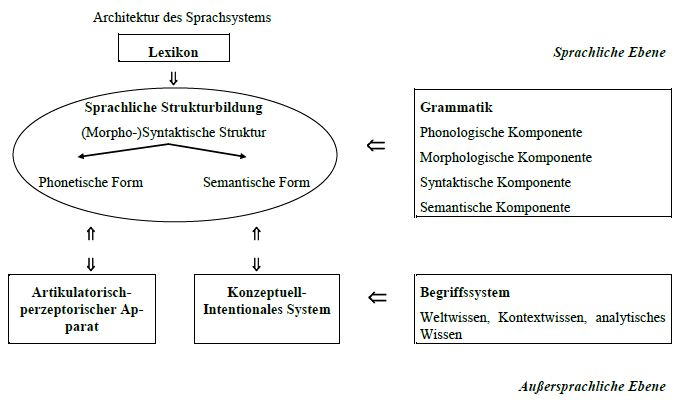
\includegraphics[scale=.3]{material/03ArchitekturSprachsystem}
%	\caption{Architektur des Sprachsystems}
%\end{figure}
%
%\end{frame}

\begin{frame}
\begin{figure}
	\centering
	
\scalebox{.72}{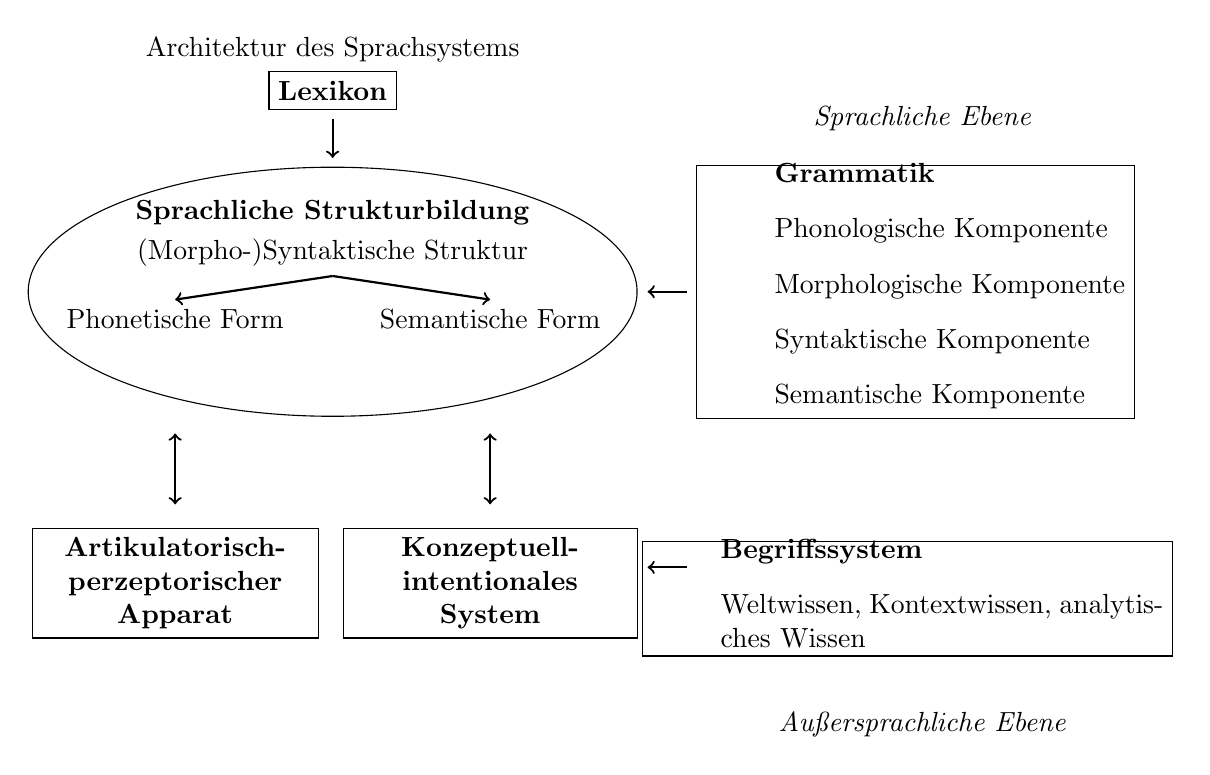
\begin{tikzpicture}
\node[above] at (0,0.3) {Architektur des Sprachsystems};
\node[below] at (0,0.3) [rectangle,draw]{\textbf{Lexikon}};
\node at (7.5,-0.3) {\textit{Sprachliche Ebene}};
\node at (7.5, -8) {\textit{Außersprachliche Ebene}};
\draw[->, thick] (0,-0.3)--(0,-0.8);
\draw (0,-2.5) ellipse (110pt and 45 pt);
\draw[->, thick] (0,-2.3)--(-2,-2.6);
\node[below] at (-2,-2.6) {Phonetische Form};
\draw[->, thick] (0,-2.3)--(2,-2.6);
\node[below] at (2,-2.6) {Semantische Form};
\node at (0,-1.5) {\textbf{Sprachliche Strukturbildung}};
\node at (0,-2) {(Morpho-)Syntaktische Struktur};
\draw[<->, thick] (-2,-4.3)--(-2,-5.2);
\draw[<->, thick] (2,-4.3)--(2,-5.2);
\draw[<-, thick] (4,-2.5)--(4.5,-2.5);
\draw[<-, thick] (4,-6)--(4.5,-6);
\node[below,text width=3.4 cm, align=center] (A) at (-2,-5.5) [rectangle, draw] {\textbf{Artikulatorisch-perzeptorischer Apparat}};
\node[below,text width=3.5 cm, align=center] (B) at (2,-5.5) [rectangle, draw] {\textbf{Konzeptuell-intentionales System}};
\node (C) at (7.4, -2.5) {\framebox
		{\begin{varwidth}{\linewidth}\begin{itemize}
			\item[] \textbf{Grammatik}
			\item[] Phonologische Komponente
			\item[] Morphologische Komponente
			\item[] Syntaktische Komponente
			\item[] Semantische Komponente
			\end{itemize}\end{varwidth}}
};
\node (D) at (7.3, -6.4) {\framebox
	{\begin{varwidth}{6.5cm}\begin{itemize}
		\item[] \textbf{Begriffssystem}
		\item[] Weltwissen, Kontextwissen, analytisches Wissen
		\end{itemize}\end{varwidth}}
};
\end{tikzpicture}}
	\caption{Architektur des Sprachsystems}
\end{figure}

\end{frame}


%%%%%%%%%%%%%%%%%%%%%%%%%%%%%%%%%%
%%%%%%%%%%%%%%%%%%%%%%%%%%%%%%%%%%
\subsubsection{Ziele der X-Bar-Theorie}

%\iftoggle{sectoc}{
%	\frame{
%		%\begin{multicols}{2}
%		\frametitle{~}
%		\tableofcontents[currentsubsection,subsubsectionstyle=hide]
%		%\end{multicols}
%	}
%}


%%%%%%%%%%%%%%%%%%%%%%%%%%%%%%%%%%
\begin{frame}
\frametitle{Ziele der X-Bar-Theorie}

\begin{itemize}
	\item Explikation der syntaktischen Beziehungen zwischen einem Kopf und seinen modifizierenden (\textbf{Adjunkten}), spezifizierenden (\textbf{Spezifikatoren}), und ergänzenden (\textbf{Argumenten}) Einheiten
	\item Explikation endozentrischer Konstruktionen
	\item Bis dahin wurden Sätze als exozentrische Konstruktionen behandelt!
\end{itemize}

\begin{figure}[b]
	\begin{minipage}[b]{0.05\textwidth}
	\end{minipage} 
	%
	\begin{minipage}[b]{0.50\textwidth}
	\centering
	\footnotesize{
		\begin{forest}
		sm edges,
		[S	[NP [Stefan,roof]]
			[VP [schreibt ein Buch,roof]]
		]
		\end{forest}
		}
		\caption{Satz vor X-Bar-Schema}	
  	\end{minipage}  
  	%  
	\begin{minipage}[b]{0.05\textwidth}
  	\end{minipage}
  	
\end{figure}

\end{frame}


%%%%%%%%%%%%%%%%%%%%%%%%%%%%%%%%%%
%%%%%%%%%%%%%%%%%%%%%%%%%%%%%%%%%%
\subsection{Strukturelle Annahmen}

\iftoggle{sectoc}{
	\frame{
		%\begin{multicols}{2}
		\frametitle{~}
		\tableofcontents[currentsubsection,subsubsectionstyle=hide]
		%\end{multicols}
	}
}

%%%%%%%%%%%%%%%%%%%%%%%%%%%%%%%%%%
\begin{frame}
\frametitle{X-Bar: Strukturelle Annahmen}

\citep[vgl.][]{Chomsky&Lasnik93a, Fries&MyP16a}

\begin{enumerate}
	\item[1.] Alle syntaktischen Phrasen haben \textbf{den gleichen syntaktischen Aufbau}.
\end{enumerate}


\begin{columns}

\begin{column}{.3\textwidth}
{\footnotesize	
\begin{itemize}
	\item XP: Phrase
	\item \MyPxbar{X}: Zwischenprojektion
	\item \zerobar{X}: Kopf
	\item YP: Spezifikator
	\item ZP: Komplement
\end{itemize}
}
\end{column}
%%
%%
\begin{column}{.7\textwidth}
\begin{figure}[b]
\centering
\begin{forest}
	MyP edges,
	[\alertred{XP} [\alertgreen{YP}]
	[\alertred{\MyPxbar{X}} [\alertred{\zerobar{X}}]
	[\alertgreen{ZP}]
	]
	]
\end{forest}
\caption{X-Bar-Schema}	
	
\end{figure}
\end{column}
	
\end{columns}

\end{frame}


%%%%%%%%%%%%%%%%%%%%%%%%%%%%%%%%%%
\begin{frame}
\frametitle{X-Bar: Strukturelle Annahmen}

	\begin{enumerate}
		\item[2.] Jede Phrase hat ein einziges, strukturell obligatorisches Element. 
		
		\ras \textbf{Kopf} der Phrase (Notation: \zerobar{X} oder X)
	\end{enumerate}

\begin{figure}[b]

\centering
\begin{forest}
	MyP edges,
	[XP [YP]
	[\MyPxbar{X} [\zerobar{X}, draw, HUred]
	[ZP]
	]
	]
\end{forest}
\caption{X-Bar-Schema}	
	
\end{figure}

\end{frame}


%%%%%%%%%%%%%%%%%%%%%%%%%%%%%%%%%%
\begin{frame}
\frametitle{X-Bar: Strukturelle Annahmen}

	\begin{enumerate}
		\item[3.] Zwischen Phrase und Kopf gibt es syntaktisch relevante Zwischenstufen 
		
		\ras \textbf{Zwischenprojektionen} (Notation: \MyPxbar{X} oder \ibar{X})
	\end{enumerate}


\begin{figure}[b]
\centering
\begin{forest}
MyP edges,
[XP 
	[YP]
	[\MyPxbar{X}, draw, HUred 
		[\zerobar{X}]
		[ZP]
	]
]
\end{forest}
\caption{X-Bar-Schema}	

\end{figure}

\end{frame}


%%%%%%%%%%%%%%%%%%%%%%%%%%%%%%%%%%
\begin{frame}
\frametitle{X-Bar: Strukturelle Annahmen}

	\begin{enumerate}
		\item[4.] Alle Nicht-Köpfe sind \textbf{maximale Projektionen} (bzw. Phrasen).
		
		\ras Notation: XP oder \xxbar{X} oder \iibar{X} oder \maxbar{X} oder  X$^2$
	\end{enumerate}

\begin{figure}[b]
\centering
\begin{forest}
	MyP edges,
	[XP [YP, draw, HUred]
	[\MyPxbar{X} [\zerobar{X}]
	[ZP, draw, HUred]
	]
	]
\end{forest}
\caption{X-Bar-Schema}	

\end{figure}

\end{frame}


%%%%%%%%%%%%%%%%%%%%%%%%%%%%%%%%%%
\begin{frame}
\frametitle{X-Bar: Strukturelle Annahmen}

	\begin{enumerate}
		\item[5.] Maximale Projektionen haben die gleiche Bar-Anzahl ($=2$).
		
		\ras Notation: XP oder \xxbar{X} oder \iibar{X} oder \maxbar{X} oder  X$^2$
	\end{enumerate}

\begin{figure}[b]
\centering
\begin{forest}
	MyP edges,
	[XP{$=$}X$^2$, draw, HUred
		[YP{$=$}Y$^2$, draw, HUred]
		[X$^1$ 
			[\zerobar{X}]
			[ZP{$=$}Z$^2$, draw, HUred]
		]
	]
\end{forest}
\caption{X-Bar-Schema}	

\end{figure}

\end{frame}



%%%%%%%%%%%%%%%%%%%%%%%%%%%%%%%%%%
\begin{frame}
\frametitle{X-Bar: Strukturelle Annahmen}

\begin{enumerate}
	\item[6.] Nur Nicht-Köpfe sind optional.
\end{enumerate}

\begin{columns}
	
\begin{column}{.5\textwidth}

\begin{figure}[b]
\centering
\begin{forest}
	MyP edges,
	[*XP [YP]
	[\MyPxbar{X} 
	[ZP]
	]
	]
\end{forest}
\caption{X-Bar-Schema}
\end{figure}
	
\end{column}
%%
%%
\begin{column}{.5\textwidth}

\begin{figure}[b]
	\centering
	\begin{forest}
		MyP edges,
		[XP 
		[\MyPxbar{X} [\zerobar{X}, draw, HUred]
		]
		]
	\end{forest}
	\caption{X-Bar-Schema}
\end{figure}
	
\end{column}

\end{columns}

\end{frame}


%%%%%%%%%%%%%%%%%%%%%%%%%%%%%%%%%%
%%%%%%%%%%%%%%%%%%%%%%%%%%%%%%%%%%
\subsection{Kopf}

\iftoggle{sectoc}{
	\frame{
		%\begin{multicols}{2}
		\frametitle{~}
		\tableofcontents[currentsubsection,subsubsectionstyle=hide]
		%\end{multicols}
	}
}


%%%%%%%%%%%%%%%%%%%%%%%%%%%%%%%%%%
\begin{frame}
\frametitle{Kopf}

\begin{itemize}
	\item Köpfe sind bereits aus der Morphologie bekannt.
\end{itemize}

\begin{figure}[b]
	\begin{minipage}[b]{0.05\textwidth}
	\end{minipage} 
	%
  	\begin{minipage}[b]{0.60\textwidth}
	\centering
	\small{
		\begin{forest}
		sm edges,
		[Auto\alertred{fahrer}
			[Auto] 
			[Fahrer]{\draw[<-,HUred] (.south east)--++(0em,-1.5ex)--++(+2em,0pt)
node[anchor=west,align=center]{Kopf};}
		]
		\end{forest}
		}
		\caption{Endozentrisches Kompositum}
  	\end{minipage}  
  	%              
	\begin{minipage}[b]{0.05\textwidth}
  	\end{minipage}
  	
\end{figure}

\begin{itemize}
	\item Der morphologische Kopf bestimmt die \textbf{morphosyntaktischen Eigenschaften} eines Wortes (Kasus, Numerus, Genus, Flexionsart, syntaktische Kategorie, auch semantische Aspekte, \dots ).
\end{itemize}

\end{frame}


%%%%%%%%%%%%%%%%%%%%%%%%%%%%%%%%%%
\begin{frame}
\frametitle{Kopf}

\begin{block}{}
Der Kopf einer Wortgruppe/""Konstituente/""Phrase/""Projektion ist dasjenige Element, das \textbf{die wichtigsten Eigenschaften} der Wortgruppe/""Konstituente/""Phrase/""Projektion bestimmt. 

Gleichzeitig steuert der Kopf den \textbf{Aufbau} der Phrase, d.\,h. der Kopf verlangt die Anwesenheit bestimmter anderer Elemente in seiner Phrase.

\citep[vgl.][]{Adger04a, MuellerS13f, MyP18b}
\end{block}

\pause

\begin{itemize}
	\item Was sind \gqq{die wichtigsten Eigenschaften}?
		\begin{itemize}
			\item Interpretation der Phrase
			\item Distribution der Phrase
			\item Morphosyntaktische Eigenschaften der Phrase
			\item Aufbau der Phrase	
		\end{itemize}
\end{itemize}

\end{frame}

%%%%%%%%%%%%%%%%%%%%%%%%%%%%%%%%%%
%%%%%%%%%%%%%%%%%%%%%%%%%%%%%%%%%%
\subsubsection{Interpretation}

%\iftoggle{sectoc}{
%	\frame{
%		%\begin{multicols}{2}
%		\frametitle{~}
%		\tableofcontents[currentsubsection,subsubsectionstyle=hide]
%		%\end{multicols}
%	}
%}

%%%%%%%%%%%%%%%%%%%%%%%%%%%%%%%%%%%
\begin{frame}
\frametitle{Interpretation}

\begin{itemize}
	\item Sehr intuitives (aber etwas unzuverlässiges) Kriterium, v.\,a. stark theorieabhängig
	\item Durch Konstituententests wissen wir, welche Wortfolgen \textbf{Konstituenten} sind.
\end{itemize}
\pause

\ea Peter kauft \alertred{[das erfrischende Wasser, das ich dir letztens empfohlen habe]}.

\pause

\settowidth\jamwidth{Vorfeldtest}
\ex \alertred{{[}Das erfrischende Wasser, das ich dir letztens empfohlen habe]} kauft Peter.  \jambox{ [\textbf{Vorfeldtest}]}

\pause

\ex \alertred{{[}Was]} kauft Peter? \ras \alertred{{[}Das erfrischende Wasser, das ich dir letztens empfohlen habe]} \jambox{ [\textbf{Fragetest}]}
\z

\pause
\begin{itemize}
	\item Aber welches Wort in einer Konstituente ist der \textbf{Kopf}?
\end{itemize} 

\end{frame}


%%%%%%%%%%%%%%%%%%%%%%%%%%%%%%%%%%
\begin{frame}
\frametitle{Interpretation}

\begin{itemize}
	\item Welches Element in den folgenden (markierten) Phrasen steuert die Interpretation?
\end{itemize}

\pause 
	
	\ea Peter kauft \alertred{[das erfrischende Wasser, das ich dir letztens empfohlen habe]}

\pause
	
	\ras \emph{Wasser} (Entität)

\pause
	\ex Peter wartet \alertred{[an der Ecke]}.

\pause
	\ras \emph{an} (Lokation)

\pause

	\ex Peter \alertred{[wartet an der Ecke]}.
	
 \pause

	\ras \emph{wartet} (Handlung)
	
	\z 
	
\end{frame}


%%%%%%%%%%%%%%%%%%%%%%%%%%%%%%%%%%
%%%%%%%%%%%%%%%%%%%%%%%%%%%%%%%%%%
\subsubsection{Distribution}

%\iftoggle{sectoc}{
%	\frame{
%		%\begin{multicols}{2}
%		\frametitle{~}
%		\tableofcontents[currentsubsection,subsubsectionstyle=hide]
%		%\end{multicols}
%	}
%}

%%%%%%%%%%%%%%%%%%%%%%%%%%%%%%%%%%%
\begin{frame}
\only<presentation>{\frametitle{Distribution}}

\begin{itemize}
	\item Der Kopf bestimmt, an welchen Positionen im Satz seine projizierte Phrase stehen kann:
	\begin{itemize}
		\item VPs: [\textbf{schläft}], [\textbf{kauft} den Wagen], [\textbf{schenkt} Maria die Blumen]
		\item NP: [\textbf{Peter}], [der \textbf{Wagen}], [der vermeintlich korrupte \textbf{Präsident} der FIFA]
		\item AP: [\textbf{nett}], [auf seinen Sohn \textbf{stolz}], [seiner Frau \textbf{treu}]
\end{itemize}
	\pause


\ea {S \ras NP $+$ VP}

\ea[]{Peter $+$ VP}
\ex[]{Peter $+$ [\textbf{schläft}].}
\ex[]{Peter $+$ [\textbf{kauft} den Wagen].}
\ex[]{Peter $+$ [\textbf{schenkt} Maria die Blumen].}
\ex[*]{Peter $+$ [der \textbf{Wagen}]}
\ex[*]{Peter $+$ [seiner Frau \textbf{treu}]}
\z

\z 
	
	
\end{itemize}

\end{frame}


%%%%%%%%%%%%%%%%%%%%%%%%%%%%%%%%%%%
\begin{frame}
\only<presentation>{\frametitle{Distribution}}

\begin{itemize}
	\item Der Kopf bestimmt, an welchen Positionen im Satz seine projizierte Phrase stehen kann:
	\begin{itemize}
		\item VPs: [\textbf{schläft}], [\textbf{kauft} den Wagen], [\textbf{schenkt} Maria die Blumen]
		\item NP: [\textbf{Peter}], [der \textbf{Wagen}], [der vermeintlich korrupte \textbf{Präsident} der FIFA]
		\item AP: [\textbf{nett}], [auf seinen Sohn \textbf{stolz}], [seiner Frau \textbf{treu}]
\end{itemize}
	\pause

\ea S \ras NP $+$ VP

\ea[]{NP $+$ parkt an der Ecke}
\ex[]{[\textbf{Peter}] $+$ parkt an der Ecke.}
\ex[]{[Der \textbf{Wagen}] $+$ parkt an der Ecke.}
\ex[]{[Der vermeintlich korrupte \textbf{Präsident} der FIFA] $+$ parkt an der Ecke.}
\ex[*]{[\textbf{Schläft}] $+$ parkt an der Ecke.}
\ex[*]{[\textbf{Nett}] $+$ parkt an der Ecke.}
\z

\z	
	
\end{itemize}

\end{frame}


%%%%%%%%%%%%%%%%%%%%%%%%%%%%%%%%%%%
\begin{frame}
\only<presentation>{\frametitle{Distribution}}

\begin{itemize}
	\item Der Kopf bestimmt, an welchen Positionen im Satz seine projizierte Phrase stehen kann:
	\begin{itemize}
		\item VPs: [\textbf{schläft}], [\textbf{kauft} den Wagen], [\textbf{schenkt} Maria die Blumen]
		\item NP: [\textbf{Peter}], [der \textbf{Wagen}], [der vermeintlich korrupte \textbf{Präsident} der FIFA]
		\item AP: [\textbf{nett}], [auf seinen Sohn \textbf{stolz}], [seiner Frau \textbf{treu}]
\end{itemize}
	\pause

\ea NP \ras Det $+$ (AP) $+$ N

\ea[]{Der $+$ AP $+$ N}
\ex[]{Der $+$ [\textbf{nette}] $+$ Onkel}
\ex[]{Der $+$ [auf seinen Sohn \textbf{stolze}] $+$ Onkel}
\ex[]{Der $+$ [seiner Frau \textbf{treue}] $+$ Onkel}
\ex[*]{Der $+$ [\textbf{schläft}] $+$ Onkel}
\ex[*]{Der $+$ [der \textbf{Wagen}] $+$ Onkel}
\z
	
\z	

\end{itemize}

\end{frame}

%%%%%%%%%%%%%%%%%%%%%%%%%%%%%%%%%%
%%%%%%%%%%%%%%%%%%%%%%%%%%%%%%%%%%
\subsubsection{Morphosyntaktische Eigenschaften}

%\iftoggle{sectoc}{
%	\frame{
%		%\begin{multicols}{2}
%		\frametitle{~}
%		\tableofcontents[currentsubsection,subsubsectionstyle=hide]
%		%\end{multicols}
%	}
%}

%%%%%%%%%%%%%%%%%%%%%%%%%%%%%%%%%%%
\begin{frame}
\only<presentation>{\frametitle{Morphosyntaktische Eigenschaften}}

\begin{itemize}
	\item \textbf{Kategorielle Zugehörigkeit} (Wortart \ras Phrasentyp)\\
	\ras Wenn der Kopf ein \textbf{Nomen} ist, ist die gesamte Phrase eine \textbf{NP}.\\
	\ras Wenn der Kopf ein \textbf{Verb} ist, ist die gesamte Phrase eine \textbf{VP}.
\end{itemize}

\begin{figure}[b]
%	\begin{minipage}[b]{0.05\textwidth}
%	\end{minipage} 
	%
	\begin{minipage}[b]{0.40\textwidth}
	\centering
	\scalebox{.68}{
	\hfill	\begin{forest}
		MyP edges,
		[VP [NP [Peter,roof]]
			[\MyPxbar{V} [NP [den Patienten,roof]]
				[V [behandelt]]		{\draw[<-,HUred] (.south east)--++(0em,-1.5ex)--++(+2em,0pt)
node[anchor=west,align=center]{Kopf};}
			]
		]
		\end{forest}
		}
		\caption{VP}	
  	\end{minipage}  
  	%  
  	\pause            
	\begin{minipage}[b]{0.05\textwidth}
		\hfill
  	\end{minipage}
  	%         
  	\begin{minipage}[b]{0.40\textwidth}
	\centering
	\scalebox{.68}{
	\hfill	\begin{forest}
		MyP edges,
		[NP [Det [Peters]]
			[\MyPxbar{N} [AP [sanfte,roof]]
				[\MyPxbar{N} [N [Behandlung]]{\draw[<-,HUred] (.south west)--++(0em,-1.5ex)--++(-2em,0pt)
node[anchor=east,align=center]{Kopf};}
					[NP [des Patienten,roof]]]]
		]
		\end{forest}
		}
		\caption{NP}
  	\end{minipage}  
  	%              
%	\begin{minipage}[b]{0.05\textwidth}
%  	\end{minipage}
  	
\end{figure}


\end{frame}


%%%%%%%%%%%%%%%%%%%%%%%%%%%%%%%%%%
\begin{frame}
\only<presentation>{\frametitle{Morphosyntaktische Eigenschaften}}

\begin{itemize}
	\item Der Kopf \textbf{projiziert} seine Merkmale auf die gesamte Phrase. 
\end{itemize}

\begin{tabular}{ll}
\textsc{Wortart} & \textsc{Merkmale}\\
\hline
\textbf{Verb}		& Wortart, Numerus-tragend, Person-tragend, Kasus-\\
					& determinierend, Verbform (Finitheitsmerkmale) \\
\hline
\textbf{Nomen}		& Wortart, Kasus-tragend, (Person), Numerus-tragend,\\
					& Genus-tragend, Genitiv-determinierend\\
\hline
\textbf{Adjektiv}	& Wortart, Kasus-tragend, Genus-tragend, Numerus-\\ 
					& tragend, Flexionsklasse, Kasus-determinierend\\
\hline
\textbf{Präposition}& Wortart, nicht-Kasus-tragend, nicht-Numerus-\\
					& tragend, nicht-Genus-tragend, Kasus-\\
					& determinierend\\					
\end{tabular}
\end{frame}


%%%%%%%%%%%%%%%%%%%%%%%%%%%%%%%%%%
%%%%%%%%%%%%%%%%%%%%%%%%%%%%%%%%%%
\subsubsection{Phrasenaufbau: Argumentstruktur}

%\iftoggle{sectoc}{
%	\frame{
%		%\begin{multicols}{2}
%		\frametitle{~}
%		\tableofcontents[currentsubsection,subsubsectionstyle=hide]
%		%\end{multicols}
%	}
%}

%%%%%%%%%%%%%%%%%%%%%%%%%%%%%%%%%%
\begin{frame}
\frametitle{Phrasenaufbau: Argumentstruktur}

\begin{itemize}
	\item Auch: Valenz, Subkategorisierung
	\item[]
	\item Es wird angenommen, dass Köpfe (lexikalische Einheiten) \ua mit ihrer Argumentstruktur im \textbf{mentalen Lexikon} gespeichert sind.
	\item[]
	\item Köpfe werden aus dem Lexikon genommen und in die \textbf{syntaktische Komponente} eingefügt, wo ihre Argumentstruktur verschiedene Ebenen im X-Bar-Schema projiziert.
\end{itemize}

\end{frame}


%%%%%%%%%%%%%%%%%%%%%%%%%%%%%%%%%%
\begin{frame}
\frametitle{Phrasenaufbau: Argumentstruktur}

\begin{block}{Argumente und Modifikatoren}
Argumente sind die von einem Kopf (Nomen, Verb, Präposition, \dots ) verlangten Einheiten, um eine wohlgeformte Phrase zu bilden. Der Kopf bestimmt dabei die \textbf{Anzahl}, die \textbf{Form} (\zB Kasus) und die \textbf{Art} (\zB Theta-Rolle) seiner Argumente. Nicht-Argumente in einer Struktur werden \textbf{Modifikatoren} genannt. Sie werden nicht verlangt, sondern können frei hinzugefügt werden und \textbf{modifizieren} die Aussage. 
\end{block}

\end{frame}


%%%%%%%%%%%%%%%%%%%%%%%%%%%%%%%%%%%
\begin{frame}
\frametitle{Phrasenaufbau: Argumentstruktur}

\begin{itemize}
	\item Der Kopf bestimmt, \textbf{welche und wieviele} Argumente \textbf{notwendig} sind, um eine wohlgeformte Phrase zu bilden.

\settowidth\jamwidth{(3 Argumente)}
\eal 
\ex {[Clara] schläft.} \jambox{(1 Argument)}
\ex {[Clara] küsst [Maria].} \jambox{(2 Argumente)}
\ex {[Maria] schenkt [Clara] [die Blumen].} \jambox{(3 Argumente)}
\zl

\pause

\eal
\ex[*]{[Clara] schläft [Maria].}
\ex[*]{[Maria] küsst [Clara] [die Blumen].}
\ex[*]{schenkt.}
\zl


\end{itemize}
\end{frame}


%%%%%%%%%%%%%%%%%%%%%%%%%%%%%%%%%%%
\begin{frame}
\only<presentation>{\frametitle{Phrasenaufbau: Argumentstruktur}}

\begin{itemize}
	\item Der Kopf bestimmt \textbf{die Form} seiner Argumente (\zB durch \textbf{Kasusrektion}).
\end{itemize}

\eal 
\ex {[Der Mann]$_{\textsc{nom}}$ schläft.}
\ex {[Der Mann]$_{\textsc{nom}}$ küsst [den Elefanten]$_{\textsc{akk}}$.}
\ex {[Der Mann]$_{\textsc{nom}}$ schenkt [dem Jungen]$_{\textsc{dat}}$ [den Elefanten]$_{\textsc{akk}}$.}
\ex {[Der Mann]$_{\textsc{nom}}$ gedenkt [des Opfers]$_{\textsc{gen}}$.}
\ex {[Der Mann]$_{\textsc{nom}}$ hilft [dem Opfer]$_{\textsc{dat}}$.}
\ex {[Der Mann]$_{\textsc{nom}}$ wartet [auf den Jungen]$_{auf}$.}
\zl

\pause

\eal
\ex[*]{[Der Mann]$_{\textsc{nom}}$ gedenkt [dem Opfer]$_{\textsc{dat}}$.}
\ex[*]{[Der Mann]$_{\textsc{nom}}$ hilft [des Opfers]$_{\textsc{gen}}$.}
\ex[*]{[Der Mann]$_{\textsc{nom}}$ wartet [den Jungen]$_{\textsc{akk}}$.}
\zl

\end{frame}


%%%%%%%%%%%%%%%%%%%%%%%%%%%%%%%%%%%
\begin{frame}
\only<presentation>{\frametitle{Phrasenaufbau: Argumentstruktur}}

\begin{itemize}
	\item Der Kopf bestimmt \textbf{die Form} seiner Argumente (\zB durch \textbf{Finitheitsrektion}).
\end{itemize}

\ea \textbf{Modalverb} verlangt Infinitiv\\
\dots dass er es \alertred{kaufen$_{\textsc{inf}}$ will}
\pause
\ex \textbf{\emph{haben}-Hilfsverb} verlangt Partizip II\\
\dots dass er es \alertred{gekauft$_{\textsc{part}}$ hat}
\pause
\ex \textbf{Modalverb} verlangt Infinitiv\\
\dots dass er es \alertred{[gekauft haben]$_{\textsc{inf}}$ will}
\pause
\ex \textbf{Modalverb} verlangt Infinitiv\\
\dots dass er es \alertred{[gekauft haben wollen]$_{\textsc{inf}}$ muss}
\pause
\ex \textbf{\emph{haben}-Hilfsverb} verlangt Partizip II\\
\dots dass er es \alertred{[gekauft haben wollen müssen/gemusst]$_{\textsc{inf}}$ hat}
\z

\end{frame}


%%%%%%%%%%%%%%%%%%%%%%%%%%%%%%%%%%%
\begin{frame}
\only<presentation>{\frametitle{Phrasenaufbau: Argumentstruktur}}

\begin{itemize}
	\item Der Kopf bestimmt \textbf{die Art}, wie seine Argumente interpretiert werden (Theta-Rollen, $\theta$-Rollen).

\eal 
\ex {[Der Elefant]$_{\textsc{agens}}$ tötet [den Mann]$_{\textsc{patiens}}$.}
\ex {[Der Elefant]$_{\textsc{thema}}$ interessierte [den Mann]$_{\textsc{experiencer}}$.}
\zl

\eal
\ex {[Peters]$_{\textsc{agens}}$ Behandlung [des Mannes]$_{\textsc{patiens}}$}
\ex {[Peters]$_{\textsc{patiens}}$ Ermordung}
\zl


	\item Einige Verben (\zB \MyPobj{regnen, schneien}) vergeben ihrem Subjekt keine Theta-Rolle. Sie sind semantisch gesehen \textbf{0-wertig}.

\end{itemize}

\end{frame}


%%%%%%%%%%%%%%%%%%%%%%%%%%%%%%%%%%
%%%%%%%%%%%%%%%%%%%%%%%%%%%%%%%%%%
\subsection{Theta-Rollen}

\iftoggle{sectoc}{
	\frame{
		%\begin{multicols}{2}
		\frametitle{~}
		\tableofcontents[currentsubsection,subsubsectionstyle=hide]
		%\end{multicols}
	}
}

%%%%%%%%%%%%%%%%%%%%%%%%%%%%%%%%%%
\begin{frame}
\frametitle{Theta-Rollen}

\begin{itemize}
	\item Auch: thematische/""semantische Rollen, Theta-Rollen, $\theta$-Rollen
\medskip	
	\item Semantische Rolle, die ein Argument von seinem Kopf erhält
\medskip	
	\item Anzahl und Definition der Theta-Rollen: theorieabhängig
\medskip

\begin{itemize}
	\item \textbf{AGENS:} jemand, der die Handlung, die durch das Prädikat bezeichnet wird, willentlich anstößt/""ausführt. \\
	\ea \alertred{[Peter]$_{\textsc{ag}}$ isst einen Kuchen.}
	\z
%	\medskip		
	\item \textbf{THEMA/""PATIENS:} jemand oder etwas, der oder das durch die vom Prädikat bezeichnete Handlung betroffen wird \\
	\ea \alertred{Peter schreibt [einen Brief]$_{\textsc{pat}}$.}
	\z
%	\medskip
	\item \textbf{EXPERIENCER:} jemand, der durch die (in der) vom Prädikat bezeichneten Handlung etwas psychisch oder physisch empfindet \\
	\ea \alertred{[Peter]$_{\textsc{exp}}$ friert.}
	\z
\end{itemize}
		

\end{itemize}

\end{frame}


%%%%%%%%%%%%%%%%%%%%%%%%%%%%%%%%%%
\begin{frame}
%\frametitle{Theta-Rollen}

\begin{itemize}
%	\item Anzahl und Definition der Theta-Rollen \ras theorieabhängig
		\item[]
	
\begin{itemize}
	
		\item \textbf{ZIEL (GOAL):} Entität, auf die die vom Prädikat ausgedrückte Handlung gerichtet ist \\
		\ea \alertred{Peter schiebt sein Auto [in die Garage]$_{\textsc{ziel}}$.}
		\z
%\medskip
		\item \textbf{ADRESSAT (SOURCE):} Entität, von der die vom Prädikat ausgedrückte Handlung ausgeht \\
		\ea \alertred{Peter fährt von [Berlin]$_{\textsc{adr}}$ nach Hamburg.}
		\z
%\medskip
		\item \textbf{ORT (LOCATION):} Ort, an dem die vom Prädikat ausgedrückte Handlung stattfindet \\
		\ea \alertred{Peter schläft [im Wohnzimmer]$_{\textsc{ort}}$.}
		\z
%\medskip
		\item \textbf{ZEIT (TIME):} Zeit(spanne), an der die vom Prädikat ausgedrückte Handlung stattfindet \\
		\ea \alertred{Peters Seminar dauerte [vier Stunden]$_{\textsc{zeit}}$.}
		\z
%\medskip
		\item \textbf{POSSESSOR:} Entität, die ein Objekt besitzt \\
		\ea \alertred{[Peter] $_{\textsc{poss}}$ hat eine Katze.}
		\z
		
\end{itemize}

\end{itemize}

\end{frame}


%%%%%%%%%%%%%%%%%%%%%%%%%%%%%%%%%%
%%%%%%%%%%%%%%%%%%%%%%%%%%%%%%%%%%
\subsection{Subkategorisierungsrahmen}

\iftoggle{sectoc}{
	\frame{
		%\begin{multicols}{2}
		\frametitle{~}
		\tableofcontents[currentsubsection,subsubsectionstyle=hide]
		%\end{multicols}
	}
}

%%%%%%%%%%%%%%%%%%%%%%%%%%%%%%%%%%
\begin{frame}
\frametitle{Subkategorisierungsrahmen}

\begin{itemize}
	\item Information im Subkategorisierungsrahmen einer Kategorie:
	\item[]
	\begin{enumerate}
		\item \textbf{Anzahl} der benötigten Argumente (syntaktische Information),
\medskip		
		\item ihre \textbf{syntaktische Kategorie} (DP, PP, CP, \dots )\\
		(syntaktische Information: c-selektionales Merkmal oder Subkategorisierungseigenschaft),
\medskip		
		\item ihre \textbf{morphosyntaktische Realisierung} (\zB Kasus) (morphologische Information),
\medskip		
		\item ihre \textbf{$\theta$-Rolle} (semantische Information),
\medskip
		\item \textbf{weitere semantische Eigenschaften}, \zB das Objekt vom Verb \MyPobj{trinken} muss \gqq{flüssig} sein (semantische Information: s-selektionales Merkmal oder 	Selektionsbeschränkung).
	\end{enumerate}
	
\end{itemize}

\end{frame}


%%%%%%%%%%%%%%%%%%%%%%%%%%%%%%%%%%
\begin{frame}
\frametitle{Subkategorisierungsrahmen}

\begin{itemize}

	\item Die Information der Argumentstruktur im Subkategorisierungsrahmen:
	
	\ea lesen: DP$_{\textsc{nom,ag}}$ (DP)$_{\textsc{akk,th}}$ $\underline{\qquad}$
	\z
	
	\item[] \textbf{$=$} \MyPobj{lesen} ist subkategorisiert für zwei Argumente, die beide syntaktisch NPn/DPn sind. Eine der NPn/DPn ist obligatorisch, wird im Nominativ realisiert und trägt die $\theta$-Rolle Agens, z.B. \MyPobj{Uta} in \MyPobj{Uta liest ein Buch}. Die andere NP/DP ist fakultativ, wird im Akkusativ realisiert und trägt die $\theta$-Rolle Thema (\zB \MyPobj{ein Buch} in \MyPobj{Uta liest ein Buch}).

	\ea schenken: DP$_{\textsc{nom,ag}}$ DP$_{\textsc{dat,ziel}}$  DP$_{\textsc{akk,th}}$ $\underline{\qquad}$ 
	\z
		
\end{itemize}

\end{frame}


%%%%%%%%%%%%%%%%%%%%%%%%%%%%%%%%%%
%%%%%%%%%%%%%%%%%%%%%%%%%%%%%%%%%%
\subsection{Modifikatoren (vs. Argumente)}

\iftoggle{sectoc}{
	\frame{
		%\begin{multicols}{2}
		\frametitle{~}
		\tableofcontents[currentsubsection,subsubsectionstyle=hide]
		%\end{multicols}
	}
}

%%%%%%%%%%%%%%%%%%%%%%%%%%%%%%%%%%
\begin{frame}

\textbf{Modifikatoren} sind vom Kopf weitgehend unabhängig in Bezug auf\dots

\begin{itemize}
	\item \textbf{Anzahl}

\eal 
\ex Maria schläft \alertred{[heute] [im Zimmer] [unruhig]}.
\ex Maria besucht Clara \alertred{[heute] [im Zimmer] [unruhig]}.
\ex Maria schenkt Clara die Blumen \alertred{[heute] [im Zimmer] [unruhig]}.
\zl

	\begin{itemize}
		\item Modifikatoren sind \textbf{immer fakultativ}!
		\item Argumente können \textbf{obligatorisch} oder \textbf{fakultativ} sein (sie werden dann \gqq{mitverstanden}: existentielle Interpretation).
		
		\eal 
		\ex Maria schläft \alertred{[heute] [im Zimmer]}.
		\ex Maria schläft \alertred{[im Zimmer]}. 
		\zl
		
		\eal 
		\ex Clara isst \alertred{[eine Schokolade]}.
		\ex Clara isst. 
		\zl
		
	\end{itemize}

\end{itemize}

\end{frame}


%%%%%%%%%%%%%%%%%%%%%%%%%%%%%%%%%%
\begin{frame}

\textbf{Modifikatoren} (syntaktisch: Adjunkte) sind vom Kopf weitgehend unabhängig in Bezug auf\dots

\begin{itemize}
	
	\item \textbf{Form}
\eal
\ex Maria schläft \alertred{[heute]$_{AdvP}$ [im Zimmer]$_{PP}$, [obwohl die Heizung nicht funktioniert]$_{CP}$}.
\ex Maria besucht Clara \alertred{[heute]$_{AdvP}$ [im Zimmer]$_{PP}$, [obwohl die Heizung nicht funktioniert]$_{CP}$}.
\ex Maria schenkt Clara die Blumen \alertred{[heute]$_{AdvP}$ [im Zimmer]$_{PP}$, [obwohl die Heizung nicht funktioniert]$_{CP}$}.
\zl

\end{itemize}

\end{frame}


%%%%%%%%%%%%%%%%%%%%%%%%%%%%%%%%%%
\begin{frame}

\textbf{Modifikatoren} (syntaktisch: Adjunkte) sind vom Kopf weitgehend unabhängig in Bezug auf\dots

\begin{itemize}
	\item \textbf{Art}

\eal 
\ex Der Ingenieur sprengte \alertred{[die Brücke]$_{\textsc{pat}}$ [heute]$_{\textsc{zeit}}$}. 
\ex Der Ingenieur sah \alertred{[die Brücke]$_{\textsc{th}}$ [heute]$_{\textsc{zeit}}$}. 
\ex Der Ingenieur verließ \alertred{[die Brücke]$_{\textsc{quelle}}$ [heute]$_{\textsc{zeit}}$}.
\zl

	\begin{itemize}
		\item Modifikatoren der gleichen Art sind \textbf{iterierbar}!
		\item Argumente der gleichen Art sind \textbf{nicht iterierbar}!
		
		\eal 
		\ex[]{Maria schläft \alertred{[heute]$_{\textsc{zeit}}$ [am frühen Morgen]$_{\textsc{zeit}}$}.}
		\ex[*]{Peter isst \alertred{[eine Schokolade]$_{\textsc{th}}$ [einen Kuchen]$_{\textsc{th}}$}.}
		\zl

		
	\end{itemize}

\end{itemize}

\end{frame}


%%%%%%%%%%%%%%%%%%%%%%%%%%%%%%%%%%
%%%%%%%%%%%%%%%%%%%%%%%%%%%%%%%%%%
\subsection{Hausaufgabe}


%%%%%%%%%%%%%%%%%%%%%%%%%%%%%%%%%%%	

	
\begin{frame}
\frametitle{Hausaufgabe}

\begin{itemize}

	\item Bestimmen Sie den Kopf der folgenden \textbf{markierten} Phrasen und begründen Sie Ihre Entscheidung:
	
	\ea\label{ex:KopfSchueler} Es geht um [\textbf{wirklich von dieser Sache überzeugte und engagierte junge Schüler, die sich dennoch über das übliche und akzeptable Ausmaß hinaus daneben benommen haben}].
	\z
	
	\ea Wir warteten auf [\textbf{den von sich sehr überzeugten Redner}].
	\z 
	
\end{itemize}

\end{frame}

%%%%%%%%%%%%%%%%%%%%%%%%%%%%%%%%%%%	

	
\begin{frame}
\frametitle{Hausaufgabe}

\begin{itemize}

	\item Geben Sie für die folgenden Wörter den Subkategorisierungsrahmen (in dem besprochenen Format) und ein(en) Beispiel(satz), der den von Ihnen angegebenen Subkategorisierungsrahmen illustriert, an:
	
	\ea übergeben
	\ex stolz
	\ex donnern
	\ex glauben
	\ex Frage
	\ex erschrecken
	\ex bemalen
	\z 
	
%	wissen, regnen, scheinen, mit, ängstigen, fürchten, Banane, Tatsache, warten, Angst, wohnen, bewohnen, auf, malen, krank, bemalen, fragen

\end{itemize}

\end{frame}

%%%%%%%%%%%%%%%%%%%%%%%%%%%%%%%%%%%	

	
\begin{frame}
\frametitle{Hausaufgabe}

\begin{itemize}
	
	\item Bestimmen Sie in den folgenden Sätzen, welche Phrasen Argumente und welche Modifikatoren des Verbs sind, und begründen Sie Ihre Entscheidung.

\end{itemize}

\ea Maria bearbeitete die Folien mit sehr viel Kreativität.

\ex Maria arbeitete an den Folien den ganzen Tag.

\ex Peter wirkte auf seinen Sohn stolz.
\z 

\end{frame}

%%%%%%%%%%%%%%%%%%%%%%%%%%%%%%%%%%%	

\iftoggle{ha-loesung}{

%%%%%%%%%%%%%%%%%%
%06d Syntax ha-loesung
%%%%%%%%%%%%%%%%%%

\begin{frame}
\frametitle{Hausaufgabe -- Lösung} 

\begin{itemize}
	\item Bestimmen Sie den Kopf der folgenden \textbf{markierten} Phrasen und begründen Sie Ihre Entscheidung:
\end{itemize}
	
	\ea Es geht um [\textbf{wirklich von dieser Sache überzeugte und engagierte junge Schüler, die sich dennoch über das übliche und akzeptable Ausmaß hinaus daneben benommen haben}].
	\z

\pause 

	
\begin{itemize}
	\item \alertgreen{Kopf: Schüler (vorläufig)}
	\item \alertgreen{Interpretation: Es geht um \emph{Schüler}}
	\item \alertgreen{Distribution: Innerhalb einer PP wird eine (DP/)NP selegiert. Der Kopf dieser NP ist das Nomen.}
	\item \alertgreen{Phrasenaufbau: Alle anderen Modifikatoren beziehen sich auf das Nomen. }
\end{itemize}

	
\end{frame}


\begin{frame}
\frametitle{Hausaufgabe -- Lösung} 

\begin{itemize}
	\item Bestimmen Sie den Kopf der folgenden Phrase und begründen Sie Ihre Entscheidung:
\end{itemize}

\ea Wir warteten auf [\textbf{den von sich sehr überzeugten Redner}].
\z 

\pause 

\begin{itemize}
	\item \alertgreen{Kopf: Redner (vorläufig)}
	\item \alertgreen{Interpretation: Es geht um \emph{Redner}}
	\item \alertgreen{Distribution: Innerhalb einer PP wird eine (DP/)NP selegiert. Der Kopf dieser NP ist das Nomen.}
	\item \alertgreen{Phrasenaufbau: Alle anderen Modifikatoren beziehen sich auf das Nomen.}
\end{itemize}
	
	
\end{frame}


\begin{frame}
\frametitle{Hausaufgabe -- Lösung} 

\begin{itemize}
	
	\item Geben Sie für die folgenden Wörter den Subkategorisierungsrahmen (in dem besprochenen Format) und ein(en) Beispiel(satz), der den von Ihnen angegebenen Subkategorisierungsrahmen illustriert, an:
	
	\settowidth \jamwidth{[Lesart 1]}
	
	\ea übergeben: \pause \alertgreen{DP$_{\textsc{nom,quelle}}$ (DP$_{\textsc{dat,ziel}}$) DP$_{\textsc{akk,th}}$ $\underline{\qquad}$} \jambox{\alertgreen{[Lesart 1]}}
	
	\alertgreen{(dass) ich Peter die Briefe \emph{übergebe}}
	\pause 
	
	\ex stolz: \pause \alertgreen{PP$_{auf+\textsc{akk,th}}$ $\underline{\qquad}$ (DP$_{\textsc{exp}}$)}
	
	\alertgreen{die auf ihre Tochter \emph{stolze} Mutter}
	\pause 
	
	\ex donnern: \pause \alertgreen{DP$_{(es),\textsc{nom}}$ $\underline{\qquad}$}
	
	\alertgreen{(dass) es \emph{donnert}}
	
	\ex glauben: \pause \alertgreen{DP$_{\textsc{nom, exp}}$ $\underline{\qquad}$ PP$_{an+\textsc{thema}}$}
	
	\alertgreen{Peter \emph{glaubt} an den Weltfrieden}
	
	\z 
	
	%	wissen, regnen, scheinen, mit, ängstigen, fürchten, Banane, Tatsache, warten, Angst, wohnen, bewohnen, auf, malen, krank, bemalen, fragen
	
\end{itemize}

\end{frame}


\begin{frame}
\frametitle{Hausaufgabe -- Lösung} 

\begin{itemize}

\item Geben Sie für die folgenden Wörter den Subkategorisierungsrahmen (in dem besprochenen Format) und ein(en) Beispiel(satz), der den von Ihnen angegebenen Subkategorisierungsrahmen illustriert, an:

\settowidth \jamwidth{[Lesart 1]}

\ea Frage: \pause \alertgreen{DP$_{\textsc{gen,ag}}$ $\underline{\qquad}$ PP$_{nach+\textsc{dat,th}}$}

\alertgreen{die Frage nach dem Schatz}
\pause 

\ex erschrecken: \pause \alertgreen{DP$_{\textsc{nom,causer}}$ DP$_{\textsc{akk,exp}}$ $\underline{\qquad}$} \jambox{\alertgreen{[Lesart 1]}}

\alertgreen{(dass) Maria Peter erschreckt}
\pause 

\ex bemalen: \pause \alertgreen{DP$_{\textsc{nom,ag}}$ DP$_{\textsc{akk,pat/th}}$ $\underline{\qquad}$}

\alertgreen{(dass) ich die Wand bemale}
\z 

%	wissen, regnen, scheinen, mit, ängstigen, fürchten, Banane, Tatsache, warten, Angst, wohnen, bewohnen, auf, malen, krank, bemalen, fragen

\end{itemize}

\end{frame}

\begin{frame}
\frametitle{Hausaufgabe -- Lösung} 

\begin{itemize}
	
	\item Bestimmen Sie in den folgenden Sätzen, welche Phrasen Argumente und welche Modifikatoren des Verbs sind, und begründen Sie Ihre Entscheidung.
	
\end{itemize}

\ea Maria bearbeitete die Folien mit sehr viel Kreativität.

\pause 
\alertgreen{Arg.: Maria, die Folien}

\alertgreen{Mod.: mit sehr viel Kreatitvität}

\alertgreen{Begründung: \dots }

\pause 


\ex Maria arbeitete an den Folien den ganzen Tag.

\pause 
\alertgreen{Arg.: Maria, an den Folien}

\alertgreen{Mod.: den ganzen Tag}

\alertgreen{Begründung: \dots }

\z 

\end{frame}


\begin{frame}
\frametitle{Hausaufgabe -- Lösung} 

\begin{itemize}

\item Bestimmen Sie in den folgenden Sätzen, welche Phrasen Argumente und welche Modifikatoren des Verbs sind, und begründen Sie Ihre Entscheidung.

\end{itemize}

\settowidth \jamwidth{[Lesart 2]}

\ea Peter wirkte auf seinen Sohn stolz. \jambox{\alertgreen{[Lesart 1]}}

\pause 
\alertgreen{Arg.: Peter, auf seinen Sohn stolz}

\alertgreen{Mod.: $\emptyset$}

\alertgreen{Begründung: \dots }

\pause 


\ex Peter wirkte auf seinen Sohn stolz. \jambox{\alertgreen{[Lesart 2]}}

\pause 
\alertgreen{Arg.: Peter, auf seinen Sohn, stolz}

\alertgreen{Mod.: $\emptyset$}

\alertgreen{Begründung: \dots }
\z 


\end{frame}
}

%%%%%%%%%%%%%%%%%%%%%%%%%%%%%%%%%%%	
 %corrupted 
%%%%%%%%%%%%%%%%%%%%%%%%%%%%%%%%%%%%%%%%%%%%%%%%
%% Compile the master file!
%% 		Slides: Antonio Machicao y Priemer
%% 		Course: GK Linguistik
%%%%%%%%%%%%%%%%%%%%%%%%%%%%%%%%%%%%%%%%%%%%%%%%


%%%%%%%%%%%%%%%%%%%%%%%%%%%%%%%%%%%%%%%%%%%%%%%%%%%%
%%%             Metadata                         
%%%%%%%%%%%%%%%%%%%%%%%%%%%%%%%%%%%%%%%%%%%%%%%%%%%%      

\title{Grundkurs Linguistik}

\subtitle{Syntax V: X-Bar-Theorie -- Lexikalische Phrasen}

\author[A. Machicao y Priemer]{
	{\small Antonio Machicao y Priemer}
	\\
	{\footnotesize \url{http://www.linguistik.hu-berlin.de/staff/amyp}}
%	\\
%	{\footnotesize \href{mailto:mapriema@hu-berlin.de}{mapriema@hu-berlin.de}}
}

\institute{Institut für deutsche Sprache und Linguistik}
  
\date{ }

%\publishers{\textbf{6. linguistischer Methodenworkshop \\ Humboldt-Universität zu Berlin}}

%\hyphenation{nobreak}


%%%%%%%%%%%%%%%%%%%%%%%%%%%%%%%%%%%%%%%%%%%%%%%%%%%%
%%%             Preamble's End                   
%%%%%%%%%%%%%%%%%%%%%%%%%%%%%%%%%%%%%%%%%%%%%%%%%%%%      


%%%%%%%%%%%%%%%%%%%%%%%%%      
\huberlintitlepage[22pt]
\iftoggle{toc}{
\frame{
\begin{multicols}{2}
	\frametitle{Inhaltsverzeichnis}\tableofcontents
	%[pausesections]
\end{multicols}
	}
	}


%%%%%%%%%%%%%%%%%%%%%%%%%%%%%%%%%%
%%%%%%%%%%%%%%%%%%%%%%%%%%%%%%%%%%
%%%%%LITERATURE:

%\nocite{Altmann&Hofmann08a}
%\nocite{Altmann93a}
\nocite{Brandt&Co06a}
\nocite{Glueck05a} 
\nocite{Grewendorf&Co91a} 
\nocite{Luedeling2009a}
\nocite{MyP18a}
\nocite{MyP18b}
\nocite{MyP18c} 
%\nocite{Meibauer&Co07a}
%\nocite{MuellerS13f}
%\nocite{MuellerS15b} 
%% Allgemein
\nocite{Glueck&Roedel16a}
\nocite{Luedeling2009a}
%\nocite{Meibauer&Co07a} 
\nocite{Repp&Co15a} 

%% Morphologie
%\nocite{Eisenberg04}

%% Syntax
\nocite{Adger04a}
%\nocite{Altmann&Hofmann08a} % Satztypen & Satzmodi
%\nocite{Altmann93a} % Satztypen & Satzmodi
\nocite{Brandt&Co06a} 
\nocite{Fanselow&Sascha87a}
\nocite{Fanselow&Sascha93a}
%\nocite{Fries&MyP16b} % Akzeptabilität
%\nocite{Fries16a} % Grammatikalität
%\nocite{Fries&MyP16d} % Kompetenz vs Performanz
\nocite{Fries&MyP16c} % GG
\nocite{Fries&MyP16a} % X-Bar-Theorie
%\nocite{Fries16e} % Satztyp
%\nocite{Fries16d} % Satzmodus 
\nocite{Grewendorf&Co91a} 
%\nocite{MyP17b} % Kerngrammatik
%\nocite{MyP18a} % Konstituententest
\nocite{MyP18b} % Kopf
\nocite{MyP18c} % Phrase
\nocite{MyP18s} % Funktionale Kategorie
\nocite{MyP18t} % Argumentstruktur
%\nocite{MuellerS13f} 
%\nocite{MuellerS15b}
\nocite{Stechow&Sternefeld88a}
\nocite{Sternefeld06a}
\nocite{Sternefeld06b}
%\nocite{Woellstein10a} % Topologisches Feldermodell
%%%%%%%%%%%%%%%%%%%%%%%%%%%%%%%%%%

\begin{frame}
\frametitle{Begleitlektüre}
	
	\begin{itemize}
		\item \textbf{obligatorisch:}
			\begin{itemize}
				\item[] AM S.~86--94
				\item[] \cite{Luedeling2009a}: Kapitel 12 \& 13 (S.~142--158)
			\end{itemize}
	\end{itemize}	
	
\end{frame}

%%%%%%%%%%%%%%%%%%%%%%%%%%%%%%%%%%
\section{Syntax V}

%%%%%%%%%%%%%%%%%%%%%%%%%%%%%%%%%%

\subsection{Einführendes}

\iftoggle{sectoc}{
	\frame{
		%\begin{multicols}{2}
		\frametitle{~}
		\tableofcontents[currentsubsection,subsubsectionstyle=hide]
		%\end{multicols}
	}
}

%%%%%%%%%%%%%%%%%%%%%%%%%%%%%%%%%%
\begin{frame}
\frametitle{Einführendes}

\begin{itemize}
	\item Organisation von natürlichen Sprachen auf:
	\begin{itemize}
		\item \textbf{lexikalischer Ebene} (Wortebene)\\
		und auf
		\item \textbf{phrasaler Ebene} (Wortgruppen, die enger zusammengehören)
\medskip		
	\end{itemize}
	\item Phrasale Organisation \ras \textbf{hierarchische} Organisation
\medskip	
	\item Alle in einem Satz auftretenden Elemente bilden Phrasen (in GG).
\medskip	
	\item Alle Phrasen haben den gleichen Aufbau (qua X-Bar-Schema)
\medskip	
	\item Unterscheidung von
	\begin{itemize}
		\item lexikalischen Phrasen \ras NP, VP, AP, (AdvP, PP)\\
		und
		\item funktionalen Phrasen \ras DP, IP, CP
	\end{itemize}
\end{itemize}

\end{frame}


%%%%%%%%%%%%%%%%%%%%%%%%%%%%%%%%%%
%%%%%%%%%%%%%%%%%%%%%%%%%%%%%%%%%%
\subsection{Lexikalische Phrasen}

\iftoggle{sectoc}{
	\frame{
		%\begin{multicols}{2}
		\frametitle{~}
		\tableofcontents[currentsubsection,subsubsectionstyle=hide]
		%\end{multicols}
	}
}

%%%%%%%%%%%%%%%%%%%%%%%%%%%%%%%%%%
\begin{frame}
\frametitle{Lexikalische Phrasen}

\begin{itemize}
	\item Maximale Projektionen, die eine \textbf{lexikalische Kategorie als Kopf} haben
\medskip	
	\item Lexikalische Kategorien haben eine konkrete \textbf{(lexikalische) Bedeutung}
\medskip	
	\item Sie sind durch produktive Wortbildungsregeln erweiterbar (\textbf{offene Klasse})
\medskip	
	\item Sie können \textbf{$\theta$-Rollen} zuweisen
\medskip	
	\item Sie können \textbf{mehrere Argumente} selegieren
\end{itemize}


\end{frame}


%%%%%%%%%%%%%%%%%%%%%%%%%%%%%%%%%%
%%%%%%%%%%%%%%%%%%%%%%%%%%%%%%%%%%
\subsubsection{Nominalphrase}
%\frame{
%\frametitle{~}
%	\tableofcontents[currentsection]
%}

%%%%%%%%%%%%%%%%%%%%%%%%%%%%%%%%%%
\begin{frame}
\frametitle{Nominalphrase}

\begin{itemize}
	\item Abk.: NP
	\item (Der Determinierer wird später analysiert.)
\end{itemize}

\begin{figure}[b]

	\begin{minipage}[b]{0.13\textwidth}
	\centering
	\scalebox{.8}{
		\begin{forest}
		MyP edges,
		[NP [\MyPxbar{N} [\zerobar{N} [Behandlung]]]]
		\end{forest}
		}
		%\caption{VP}	
  	\end{minipage}  
  	%  
  	\pause            
	\begin{minipage}[b]{0.02\textwidth}
	\hfill
  	\end{minipage}
  	%         
  	\begin{minipage}[b]{0.30\textwidth}
	\centering
	\scalebox{.8}{
		\begin{forest}
		MyP edges,
		[NP [\MyPxbar{N}	[\zerobar{N} [Behandlung]]
					 	[DP [des Patienten,roof]]
			]
		]			 
		\end{forest}
		}
		%\caption{NP}
  	\end{minipage}  
  	%              
	\begin{minipage}[b]{0.02\textwidth}
	\hfill
  	\end{minipage}
  	%  
  	\pause            
	\begin{minipage}[b]{0.41\textwidth}
	\centering
	\scalebox{.8}{
		\begin{forest}
		MyP edges,
		[NP [AP [effektive,roof]]
			[NP 
		    [\MyPxbar{N}	[\zerobar{N} [Behandlung]]
					 	[DP [des Patienten,roof]]
			]]
		]			 
		\end{forest}
		}
		%\caption{Adjunkt und Komplement}	
  	\end{minipage}
  	%         
\end{figure}
\end{frame}


%%%%%%%%%%%%%%%%%%%%%%%%%%%%%%%%%%
%%%%%%%%%%%%%%%%%%%%%%%%%%%%%%%%%%
\subsubsection{Adjektivphrase}
%\frame{
%\frametitle{~}
%	\tableofcontents[currentsection]
%}

%%%%%%%%%%%%%%%%%%%%%%%%%%%%%%%%%%
\begin{frame}
\frametitle{Adjektivphrase}

\begin{itemize}
	\item Abk.: AP
\end{itemize}

\begin{figure}[b]
%	\begin{minipage}[b]{0.05\textwidth}
%	\end{minipage} 
%	%
	\begin{minipage}[b]{0.18\textwidth}
	\centering
	\footnotesize{
		\begin{forest}
		MyP edges,
		[AP [\MyPxbar{A} [\zerobar{A} [stolz]]]]
		\end{forest}
		}
		%\caption{VP}	
  	\end{minipage}  
  	%  
  	\pause            
	\begin{minipage}[b]{0.03\textwidth}
	\hfill
  	\end{minipage}
  	%         
  	\begin{minipage}[b]{0.30\textwidth}
	\centering
	\footnotesize{
		\begin{forest}
		MyP edges,
		[AP [\MyPxbar{A}	[PP [auf seine Tochter,roof]]
						[\zerobar{A} [stolz]]
			]
		]			 
		\end{forest}
		}
		%\caption{NP}
  	\end{minipage}  
  	%              
	\begin{minipage}[b]{0.03\textwidth}
	\hfill
  	\end{minipage}
  	%  
  	\pause            
	\begin{minipage}[b]{0.41\textwidth}
	\centering
	\footnotesize{
		\begin{forest}
		MyP edges,
		[AP [AdvP [sehr,roof]]
			[AP 
		    [\MyPxbar{A}	[PP [auf seine Tochter,roof]]				
		    			[\zerobar{A} [stolz]]
			]]
		]			 
		\end{forest}
		}
		%\caption{Adjunkt und Komplement}	
  	\end{minipage}
  	%         
\end{figure}
\end{frame}


%%%%%%%%%%%%%%%%%%%%%%%%%%%%%%%%%%
%%%%%%%%%%%%%%%%%%%%%%%%%%%%%%%%%%
\subsubsection{Adverbialphrase}
%\frame{
%\frametitle{~}
%	\tableofcontents[currentsection]
%}

%%%%%%%%%%%%%%%%%%%%%%%%%%%%%%%%%%
\begin{frame}
\frametitle{Adverbialphrase}

\begin{itemize}
	\item Abk.: AdvP
\end{itemize}

\begin{figure}[b]
%	\begin{minipage}[b]{0.05\textwidth}
%	\end{minipage} 
%	%
	\begin{minipage}[b]{0.18\textwidth}
	\centering
	\footnotesize{
		\begin{forest}
		MyP edges,
		[AdvP [\MyPxbar{Adv} [\zerobar{Adv} [oft]]]]
		\end{forest}
		}
		%\caption{VP}	
  	\end{minipage}  
  	%  
  	\pause            
	\begin{minipage}[b]{0.03\textwidth}
	\hfill
  	\end{minipage}
  	%         
	\begin{minipage}[b]{0.41\textwidth}
	\centering
	\footnotesize{
		\begin{forest}
		MyP edges,
		[\alertgreen{AdvP} [AdvP [sehr,roof]]
			[\alertgreen{AdvP} 
		    [\alertgreen{\MyPxbar{Adv}}	[\alertgreen{\zerobar{Adv}} [oft]]
			]]
		]			 
		\end{forest}
		}
		%\caption{Adjunkt und Komplement}	
  	\end{minipage}
  	%         
\end{figure}
\end{frame}


%%%%%%%%%%%%%%%%%%%%%%%%%%%%%%%%%%
%%%%%%%%%%%%%%%%%%%%%%%%%%%%%%%%%%
\subsubsection{Prä- \& Postpositionalphrase}
%\frame{
%\frametitle{~}
%	\tableofcontents[currentsection]
%}

%%%%%%%%%%%%%%%%%%%%%%%%%%%%%%%%%%
\begin{frame}
\frametitle{Prä- \& Postpositionalphrase}

\begin{itemize}
	\item \textbf{Präpositionalphrase} \ras PP
	\item \textbf{Postpositionalphrase} \ras PostP
	\item In unserem Seminar: PP für beide
\end{itemize}

\begin{figure}[b]
%	\begin{minipage}[b]{0.05\textwidth}
%	\end{minipage} 
%	%
  	\begin{minipage}[b]{0.30\textwidth}
	\centering
	\footnotesize{
		\begin{forest}
		MyP edges,
		[PP [\MyPxbar{P}
				[\zerobar{P} [mit]]
				[DP [dem Finger,roof]]
			]
		]
		\end{forest}
		}
		%\caption{NP}
  	\end{minipage}  
  	%              
  	\pause            
	\begin{minipage}[b]{0.30\textwidth}
	\centering
	\footnotesize{
		\begin{forest}
		MyP edges,
		[PostP [\MyPxbar{Post} [DP [der Syntax,roof]]
							[\zerobar{Post} [wegen]]]
		]	 
		\end{forest}
		}
		%\caption{Adjunkt und Komplement}	
  	\end{minipage}
  	%
 	\pause            
	\begin{minipage}[b]{0.30\textwidth}
	\centering
	\footnotesize{
		\begin{forest}
		MyP edges,
		[PP
		[AdvP [kurz,roof]]
		[PP [\MyPxbar{P}
				[\zerobar{P} [vor]]
				[DP [dem Haus,roof]]
			]
		]]
		\end{forest}
		}
		%\caption{NP}
  	\end{minipage}  
  	%                       
\end{figure}
\end{frame}


%%%%%%%%%%%%%%%%%%%%%%%%%%%%%%%%%%
%%%%%%%%%%%%%%%%%%%%%%%%%%%%%%%%%%
\subsubsection{Verbalphrase}
%\frame{
%\frametitle{~}
%	\tableofcontents[currentsection]
%}

%%%%%%%%%%%%%%%%%%%%%%%%%%%%%%%%%%
\begin{frame}
\frametitle{Verbalphrase}

\begin{itemize}
	\item Abk.: VP
	\item \textbf{Kopf} der VP \ras rechtsperipher 
\end{itemize}

\begin{figure}[b]
%	\begin{minipage}[b]{0.05\textwidth}
%	\end{minipage} 
%	%
	\begin{minipage}[b]{0.18\textwidth}
	\centering
	\footnotesize{
		\begin{forest}
		MyP edges,
		[VP [\MyPxbar{V} [\zerobar{V} [schlafen]]]]
		\end{forest}
		}
		%\caption{VP}	
  	\end{minipage}  
  	%  
  	\pause            
	\begin{minipage}[b]{0.03\textwidth}
	\hfill
  	\end{minipage}
  	%         
  	\begin{minipage}[b]{0.30\textwidth}
	\centering
	\footnotesize{
		\begin{forest}
		MyP edges,
		[VP [\MyPxbar{V}	[DP [den Wagen,roof]]
						[\zerobar{V} [kaufen]]
			]
		]			 
		\end{forest}
		}
		%\caption{NP}
  	\end{minipage}  
  	%              
	\begin{minipage}[b]{0.03\textwidth}
	\hfill
  	\end{minipage}
  	%  
  	\pause            
	\begin{minipage}[b]{0.41\textwidth}
	\centering
	\footnotesize{
		\begin{forest}
		MyP edges,
		[VP [AdvP [schnell,roof]]
			[VP 
		    [\MyPxbar{V}	[DP [den Wagen,roof]]				
		    			[\zerobar{V} [kaufen]]
			]]
		]			 
		\end{forest}
		}
		%\caption{Adjunkt und Komplement}	
  	\end{minipage}
  	%         
\end{figure}

\end{frame}


%%%%%%%%%%%%%%%%%%%%%%%%%%%%%%%%%%
\begin{frame}
\frametitle{Verbalphrase}

\begin{itemize}
	\item \textbf{Transitive} und \textbf{ditransitive} Verbalphrase
	\item \textbf{Kopf} der VP \ras rechtsperipher 
\end{itemize}

\begin{figure}[b]
%	\begin{minipage}[b]{0.05\textwidth}
%	\end{minipage} 
%	%
	\begin{minipage}[b]{0.4\textwidth}
	\centering
	\scalebox{.8}{
		\begin{forest}
		sm edges,
		[VP [AdvP [schnell,roof]]
			[VP 
		    [\MyPxbar{V}	[DP [\alertblue{den Wagen},roof]]				
		    			[\zerobar{V} [kaufen]]
			]]
		]			 
		\end{forest}
		}
		\caption{Transitive VP}	
  	\end{minipage} 
%  	  %
%  	\pause            
%	\begin{minipage}[b]{0.01\textwidth}
%	\hfill
%  	\end{minipage}
%  	  %
	\begin{minipage}[b]{0.52\textwidth}
	\centering
	\scalebox{.8}{
		\begin{forest}
		sm edges,
		[VP [AdvP [schnell,roof]]
			[VP 
				[DP [\alertgreen{dem Jungen},roof]]
				[\MyPxbar{V}	
					[DP [\alertblue{den Wagen},roof]]				
		    		[\zerobar{V} [schenken]]
			]]
		]			 
		\end{forest}
		}
		\caption{Ditransitive VP}	
  	\end{minipage}
  	%         
\end{figure}

\end{frame}

%%%%%%%%%%%%%%%%%%%%%%%%%%%%%%%%%%%%%%%%%%%%%%%%%%%%%

\begin{frame}
\frametitle{Verbalphrase}

\begin{itemize}
	\item Die Position der Elemente in Phrasen ist \textbf{strukturell} bestimmt
	%	\item[]
	\item Position \ras \textbf{Funktion} 
	%	\item[]
	\item Die (Basis)Position wird von der Struktur bestimmt und ist im Subkategorisierungsrahmen kodiert:
	%	\item[]
	\item[] \textbf{schenken:} {\small DP$_{\textsc{nom,ag}}$ DP$_{\textsc{dat,ziel}}$  DP$_{\textsc{akk,th}}$ $\underline{\qquad}$ }
	\item[]
	\item Deutsch \ras SOV-Sprache (später mehr dazu!)
\end{itemize}

\end{frame}

%%%%%%%%%%%%%%%%%%%%%%%%%%%%%%%%%%
\begin{frame}
\frametitle{Verbalphrase}

\begin{figure}[b]

	\begin{minipage}[b]{0.50\textwidth}
	\begin{itemize}

		\item Position \ras \textbf{Funktion} 

		\item[] \textbf{schenken:}\\
		{\small \alertred{DP$_{\textsc{nom,ag}}$} DP$_{\textsc{dat,ziel}}$  DP$_{\textsc{akk,th}}$ $\underline{\qquad}$ }

	\end{itemize}
\end{minipage}  
  	%  
  	%  
	\begin{minipage}[b]{0.48\textwidth}
	\centering
	\footnotesize{
		\begin{forest}
		MyP edges,
		[?P [DP [Die Dame,roof]],tikz={\node [draw,HUred,fit=()] {};} 
			[\MyPxbar{?} 		
		[VP [AdvP [schnell,roof]]
			[VP [DP [dem Jungen,roof]]
		    [\MyPxbar{V}	[DP [den Wagen,roof]]				
		    			[\zerobar{V} [schenken]]
			]]
		]
			[\zerobar{?}]
		]]			 
		\end{forest}
		}
%		%\caption{Adjunkt und Komplement}	
  	\end{minipage}
%  	%         
\end{figure}

\end{frame}

%%%%%%%%%%%%%%%%%%%%%%%%%%%%%%%%%%
\begin{frame}
\frametitle{Verbalphrase}

\begin{figure}[b]

	\begin{minipage}[b]{0.50\textwidth}
	\begin{itemize}

	\item Position \ras \textbf{Funktion} 

	\item[] \textbf{schenken:}\\
	{\small DP$_{\textsc{nom,ag}}$ \alertred{DP$_{\textsc{dat,ziel}}$}  DP$_{\textsc{akk,th}}$ $\underline{\qquad}$ }
	\item[]

	\end{itemize}
  	\end{minipage}  
  	%  
  	%  
	\begin{minipage}[b]{0.48\textwidth}
	\centering
	\footnotesize{
		\begin{forest}
		MyP edges,
		[?P [DP [Die Dame,roof]]
			[\MyPxbar{?} 		
		[VP [AdvP [schnell,roof]]
			[VP [DP [dem Jungen,roof]],tikz={\node [draw,HUred,fit=()] {};}
		    [\MyPxbar{V}	[DP [den Wagen,roof]]				
		    			[\zerobar{V} [schenken]]
			]]
		]
			[\zerobar{?}]
		]]			 
		\end{forest}
		}
		%\caption{Adjunkt und Komplement}	
  	\end{minipage}
  	%         
\end{figure}

\end{frame}


%%%%%%%%%%%%%%%%%%%%%%%%%%%%%%%%%%
\begin{frame}
\frametitle{Verbalphrase}

\begin{figure}[b]

	\begin{minipage}[b]{0.50\textwidth}
	\begin{itemize}

	\item Position \ras \textbf{Funktion} 

	\item[] \textbf{schenken:}\\
	{\small DP$_{\textsc{nom,ag}}$ DP$_{\textsc{dat,ziel}}$ \alertred{DP$_{\textsc{akk,th}}$} $\underline{\qquad}$ }

	\end{itemize}
  	\end{minipage}  
  	%  
  	%  
	\begin{minipage}[b]{0.48\textwidth}
	\centering
	\footnotesize{
		\begin{forest}
		MyP edges,
		[?P [DP [Die Dame,roof]]
			[\MyPxbar{?} 		
		[VP [AdvP [schnell,roof]]
			[VP [DP [dem Jungen,roof]]
		    [\MyPxbar{V}	[DP [den Wagen,roof]],tikz={\node [draw,HUred,fit=()] {};}				
		    			[\zerobar{V} [schenken]]
			]]
		]
			[\zerobar{?}]
		]]			 
		\end{forest}
		}
		%\caption{Adjunkt und Komplement}	
  	\end{minipage}
  	%         
\end{figure}

\end{frame}


%%%%%%%%%%%%%%%%%%%%%%%%%%%%%%%%%%
\begin{frame}
\frametitle{Verbalphrase}

\begin{figure}[b]

	\begin{minipage}[b]{0.50\textwidth}
	\begin{itemize}

	\item Position \ras \textbf{Funktion} 

	\item[] \textbf{schenken:}\\
	{\footnotesize DP$_{\textsc{nom,ag}}$ DP$_{\textsc{dat,ziel}}$ DP$_{\textsc{akk,th}}$ \alertred{$\underline{schenken}$} }

	\end{itemize}
  	\end{minipage}  
  	%  
  	%  
	\begin{minipage}[b]{0.48\textwidth}
	\centering
	\footnotesize{
		\begin{forest}
		MyP edges,
		[?P [DP [Die Dame,roof]]
			[\MyPxbar{?} 		
		[VP [AdvP [schnell,roof]]
			[VP [DP [dem Jungen,roof]]
		    [\MyPxbar{V}	[DP [den Wagen,roof]]				
		    			[\zerobar{V} [schenken]],tikz={\node [draw,HUred,fit=()] {};}
			]]
		]
			[\zerobar{?}]
		]]			 
		\end{forest}
		}
		%\caption{Adjunkt und Komplement}	
  	\end{minipage}
  	%         
\end{figure}

\end{frame}


%%%%%%%%%%%%%%%%%%%%%%%%%%%%%%%%%%
%%%%%%%%%%%%%%%%%%%%%%%%%%%%%%%%%%
\subsection{Hausaufgabe}
%\frame{
%\frametitle{~}
%	\tableofcontents[currentsection]
%}

%%%%%%%%%%%%%%%%%%%%%%%%%%%%%%%%%%
\begin{frame}
\frametitle{Hausaufgabe}

\begin{itemize}
	\item Analysieren Sie die folgende Phrase nach dem X-Bar-Schema. Verwenden Sie dabei \textbf{keine Abkürzungen}!
\end{itemize}

\ea kurz vor Weihnachten Otto schöne Blumen schenken
\z

\end{frame}

%%%%%%%%%%%%%%%%%%%%%%%%%%%%%%%%%%%%%%%%%%%%%%%%%%%

\iftoggle{ha-loesung}{
	
%%%%%%%%%%%%%%%%%%%%%%%%%
%06e syntax ha-loesung
%%%%%%%%%%%%%%%%%%%%%%%%%

\begin{frame}
\frametitle{Hausaufgabe -- Lösung}

\begin{figure}[b]
	\centering
	\scalebox{.65}{
		\begin{forest}
		MyP edges,
		[\alertgreen{VP} [\alertgreen{PP} [\alertgreen{AdvP} [\alertgreen{\MyPxbar{Adv}} [\alertgreen{\zerobar{Adv}} [\alertgreen{kurz}]]]]
				[\alertgreen{PP} [\alertgreen{\MyPxbar{P}} 	[\alertgreen{\zerobar{P}} [\alertgreen{vor}]]
								[\alertgreen{NP} [\alertgreen{\MyPxbar{N}}[\alertgreen{\zerobar{N}}[\alertgreen{Weihnachten}]]]]]]]
			[\alertgreen{VP} [\alertgreen{NP} [\alertgreen{\MyPxbar{N}}[\alertgreen{\zerobar{N}} [\alertgreen{Otto}]]] ]
				[\alertgreen{\MyPxbar{V}} 	[\alertgreen{NP} [\alertgreen{AP} [\alertgreen{\MyPxbar{A}} [\alertgreen{\zerobar{A}} [\alertgreen{schöne}]]]]
								[\alertgreen{NP} [\alertgreen{\MyPxbar{N}} [\alertgreen{\zerobar{N}} [\alertgreen{Blumen}]]]]]
							[\alertgreen{\zerobar{V}} [\alertgreen{schenken}]]]
			]
		]			 
		\end{forest}
		}
		\caption{Vorläufige Struktur!}	
  
\end{figure}

\end{frame}

}


%%%%%%%%%%%%%%%%%%%%%%%%%%%%%%%%%%
%%%%%%%%%%%%%%%%%%%%%%%%%%%%%%%%%%
\subsection{Schlusswort}
%\frame{
%\frametitle{~}
%	\tableofcontents[currentsection]
%}

%%%%%%%%%%%%%%%%%%%%%%%%%%%%%%%%%%%
\begin{frame}
\frametitle{Schlusswort: The Awful German Language}

\begin{scriptsize}

%\begin{quote}
There are ten parts of speech, and they are all troublesome. An average sentence, in a German newspaper, is a sublime and impressive curiosity; it occupies a quarter of a column; it contains all the ten parts of speech -- not in regular order, but mixed; it is built mainly of compound words constructed by the writer on the spot, and not to be found in any dictionary -- six or seven words compacted into one, without joint or seam -- that is, without hyphens; it treats of fourteen or fifteen different subjects, each enclosed in a parenthesis of its own, with here and there extra parentheses, which re-enclose three or four of the minor parentheses, making pens with pens; finally, all the parentheses and re-parentheses are massed together between a couple of king-parentheses, one of which is placed in the first line of the majestic sentence and the other in the middle of the last line of it -- \emph{after which comes the verb}, and you find out for the first time what the man has been talking about; and after the verb -- merely by way of ornament, as far as I can make out, -- the writer shovels in ``\emph{haben sind gewesen gehabt haben geworden sein},'' or words to that effect, and the monument is finished. I suppose that this closing hurrah is in the nature of the flourish to a man's signature -- not necessary, but pretty. German books are easy enough to read when you hold them before the looking-glass or stand on your head,-- so as to reverse the construction, -- but I think that to learn to read and understand a German newspaper is a thing which must always remain an impossibility to a foreigner.
%\end{quote}

\hfill \citep{Twain10b}
\end{scriptsize}

\end{frame}

%%%%%%%%%%%%%%%%%%%%%%%%%%%%%%%%%%%%%%%%%%%%%%%%
%% Compile the master file!
%% 		Slides: Antonio Machicao y Priemer
%% 		Course: GK Linguistik
%%%%%%%%%%%%%%%%%%%%%%%%%%%%%%%%%%%%%%%%%%%%%%%%


%%%%%%%%%%%%%%%%%%%%%%%%%%%%%%%%%%%%%%%%%%%%%%%%%%%%
%%%             Metadata                         
%%%%%%%%%%%%%%%%%%%%%%%%%%%%%%%%%%%%%%%%%%%%%%%%%%%%      

\title{Grundkurs Linguistik}

\subtitle{Syntax VI: X-Bar-Theorie -- Funktionale Phrasen I}

\author[A. Machicao y Priemer]{
	{\small Antonio Machicao y Priemer}
	\\
	{\footnotesize \url{http://www.linguistik.hu-berlin.de/staff/amyp}}
%	\\
%	{\footnotesize \href{mailto:mapriema@hu-berlin.de}{mapriema@hu-berlin.de}}
}

\institute{Institut für deutsche Sprache und Linguistik}

\date{ }

%\publishers{\textbf{6. linguistischer Methodenworkshop \\ Humboldt-Universität zu Berlin}}

%\hyphenation{nobreak}


%%%%%%%%%%%%%%%%%%%%%%%%%%%%%%%%%%%%%%%%%%%%%%%%%%%%
%%%             Preamble's End                   %%%
%%%%%%%%%%%%%%%%%%%%%%%%%%%%%%%%%%%%%%%%%%%%%%%%%%%%      


%%%%%%%%%%%%%%%%%%%%%%%%%      
\huberlintitlepage[22pt]
\iftoggle{toc}{
\frame{
\begin{multicols}{2}
	\frametitle{Inhaltsverzeichnis}\tableofcontents
	%[pausesections]
\end{multicols}
	}
	}


%%%%%%%%%%%%%%%%%%%%%%%%%%%%%%%%%%
%%%%%%%%%%%%%%%%%%%%%%%%%%%%%%%%%%
%%%%%LITERATURE:

%\nocite{Altmann&Hofmann08a}
%\nocite{Altmann93a}
\nocite{Brandt&Co06a}
\nocite{Glueck05a} 
\nocite{Grewendorf&Co91a} 
\nocite{Luedeling2009a} 
%\nocite{Meibauer&Co07a}
\nocite{MuellerS13f} 
\nocite{MuellerS15b}
%% Allgemein
\nocite{Glueck&Roedel16a}
%\nocite{Meibauer&Co07a} 
\nocite{Repp&Co15a} 

%% Morphologie
%\nocite{Eisenberg04}

%% Syntax
\nocite{Adger04a}
%\nocite{Altmann&Hofmann08a} % Satztypen & Satzmodi
%\nocite{Altmann93a} % Satztypen & Satzmodi
\nocite{Brandt&Co06a} 
\nocite{Fanselow&Sascha87a}
\nocite{Fanselow&Sascha93a}
%\nocite{Fries&MyP16b} % Akzeptabilität
%\nocite{Fries16a} % Grammatikalität
%\nocite{Fries&MyP16d} % Kompetenz vs Performanz
\nocite{Fries&MyP16c} % GG
\nocite{Fries&MyP16a} % X-Bar-Theorie
%\nocite{Fries16e} % Satztyp
%\nocite{Fries16d} % Satzmodus 
\nocite{Grewendorf&Co91a} 
%\nocite{MyP17b} % Kerngrammatik
%\nocite{MyP18a} % Konstituententest
\nocite{MyP18b} % Kopf
\nocite{MyP18c} % Phrase
\nocite{MyP18s} % Funktionale Kategorie
\nocite{MyP18t} % Argumentstruktur
%\nocite{MuellerS13f} 
%\nocite{MuellerS15b}
\nocite{Stechow&Sternefeld88a}
\nocite{Sternefeld06a}
\nocite{Sternefeld06b}
%\nocite{Woellstein10a} % Topologisches Feldermodell
%%%%%%%%%%%%%%%%%%%%%%%%%%%%%%%%%

\begin{frame}
\frametitle{Begleitlektüre}

	\begin{itemize}
		\item \textbf{obligatorisch:}
			\begin{itemize}
				\item[] AM S.~86--94
				\item[] \cite{Luedeling2009a}: Kapitel 12 \& 13 (S.~142--158)
			\end{itemize}
	\end{itemize}

\end{frame}

%%%%%%%%%%%%%%%%%%%%%%%%%%%%%%%%%
\section{Syntax VI}
%%%%%%%%%%%%%%%%%%%%%%%%%%%%%%%%%

\subsection{Begriffe: GG vs. Traditionell}

\iftoggle{sectoc}{
	\frame{
		%\begin{multicols}{2}
		\frametitle{~}
		\tableofcontents[currentsubsection,subsubsectionstyle=hide]
		%\end{multicols}
	}
}


%%%%%%%%%%%%%%%%%%%%%%%%%%%%%%%%%%%
\begin{frame}
\frametitle{Begriffe: GG \vs Traditionell}

\begin{itemize}
	\item Die Begriffe in der \textbf{traditionellen Grammatik} (UE) und in anderen syntaktischen Theorien (Valenz, \textbf{GG}, \dots ) sind nicht vollkommen gleichzusetzen, weil sie auch nicht die gleichen \textbf{Kategorien} bezeichnen!
\medskip	
	\item Es gibt Bereiche, in denen die Begriffe Ähnliches bezeichnen, aber \idR  haben sie verschiedene Reichweiten.
\medskip	
	\item Kurze Gegenüberstellung zur begrifflichen Klärung \dots
\medskip	
	\item $\approx$ \ras ungefähr
\end{itemize}

\end{frame}


%%%%%%%%%%%%%%%%%%%%%%%%%%%%%%%%%%
\begin{frame}
\frametitle{Begriffe: GG \vs Traditionell}

\begin{minipage}[b]{0.47\textwidth}

	\textbf{GG:}

	\begin{itemize}
		\item \alertred{\textbf{Argumente:}}
		\begin{itemize}
			\item (aus der Semantik entlehnter Begriff)
			
			\item Leerstellen einer Kategorie \zerobar{X}
			
			\item \textbf{Externes Argument + Komplemente}
		\end{itemize}
\medskip
		\item \textbf{Komplemente:}
		\begin{itemize}
			\item interne Argumente
		\end{itemize}

	\end{itemize}	
\end{minipage}  
  	  %
  	  %
\begin{minipage}[b]{0.5\textwidth}
	\begin{figure}
	\centering
	\scalebox{.55}{
		\begin{forest}
		sm edges,
		[?P [DP [Die Dame,roof]],tikz={\node [draw,HUred,fit=()] {};} 
			[\MyPxbar{?} 		
		[VP [AdvP [schnell,roof]]
			[VP [DP [dem Jungen,roof]],tikz={\node [draw,HUred,fit=()] {};}
		    [\MyPxbar{V}	[DP [den Wagen,roof]],tikz={\node [draw,HUred,fit=()] {};}				
		    			[\zerobar{V} [schenken]]
			]]
		]
			[\zerobar{?} [~]]
		]]			 
		\end{forest}
		}         
	\end{figure}
\end{minipage}

\end{frame}


%%%%%%%%%%%%%%%%%%%%%%%%%%%%%%%%%%
\begin{frame}
\frametitle{Begriffe: GG \vs Traditionell}

\begin{minipage}[b]{0.47\textwidth}

	\textbf{GG:}

	\begin{itemize}
		\item \textbf{Argumente:}
		\begin{itemize}
			\item (aus der Semantik entlehnter Begriff)
			
			\item Leerstellen einer Kategorie \zerobar{X}
			
			\item \textbf{Externes Argument + Komplemente}
		\end{itemize}	
\medskip		
		\item \alertred{\textbf{Komplemente:}}
		\begin{itemize}
			\item interne Argumente
		\end{itemize}
		
	\end{itemize}	
\end{minipage}  
  	%  
  	%  
\begin{minipage}[b]{0.48\textwidth}
	\begin{figure}
	\centering
	\scalebox{.55}{
		\begin{forest}
		sm edges,
		[?P [DP [Die Dame,roof]]
			[\MyPxbar{?} 		
		[VP [AdvP [schnell,roof]]
			[\alertred{VP} [DP [dem Jungen,roof]],tikz={\node [draw,HUred,fit=()] {};}
		    [\MyPxbar{V}	[DP [den Wagen,roof]],tikz={\node [draw,HUred,fit=()] {};}				
		    			[\zerobar{V} [schenken]]
			]]
		]
			[\zerobar{?} [~]]
		]]			 
		\end{forest}
		}

	\end{figure}
\end{minipage}

\end{frame}


%%%%%%%%%%%%%%%%%%%%%%%%%%%%%%%%%%
\begin{frame}
\frametitle{Begriffe: GG \vs Traditionell}

\begin{minipage}[b]{0.47\textwidth}

	\textbf{GG:}

	\begin{itemize}
		\item \alertred{\textbf{Externes Argument:}}\\
		Argument von \zerobar{X}, dessen Basisposition \textbf{außerhalb} der XP liegt
\medskip
		\item \textbf{Internes Argument:}\\
		Argument von \zerobar{X}, dessen Basisposition \textbf{innerhalb} der XP liegt
	\end{itemize}	
\end{minipage}  
  	%  
  	%  
\begin{minipage}[b]{0.48\textwidth}
	\begin{figure}
	\centering
	\scalebox{.55}{
		\begin{forest}
		sm edges,
		[\alertred{?P} [DP [Die Dame,roof]],tikz={\node [draw,HUred,fit=()] {};}
			[\MyPxbar{?} 		
		[VP [AdvP [schnell,roof]]
			[\alertgreen{VP} [DP [dem Jungen,roof]]
		    [\MyPxbar{V}	[DP [den Wagen,roof]]
		    			[\zerobar{V} [schenken]]
			]]
		]
			[\zerobar{?} [~]]
		]]			 
		\end{forest}
		}
	\end{figure}
\end{minipage}    

\end{frame}


%%%%%%%%%%%%%%%%%%%%%%%%%%%%%%%%%%
\begin{frame}
\frametitle{Begriffe: GG \vs Traditionell}

\begin{minipage}[b]{0.47\textwidth}

	\textbf{GG:}
	\begin{itemize}
		\item \textbf{Externes Argument:}\\
		Argument von \zerobar{X}, dessen Basisposition \textbf{außerhalb} der XP liegt
\medskip
		\item \textbf{Internes Argument:}\\
		Argument von \zerobar{X}, dessen Basisposition \textbf{innerhalb} der XP liegt
	\end{itemize}	
\end{minipage}  
  	%  
  	%  
\begin{minipage}[b]{0.48\textwidth}
	\begin{figure}
	\centering
	\scalebox{.55}{
		\begin{forest}
		sm edges,
		[?P [DP [Die Dame,roof]]
			[\MyPxbar{?} 		
		[VP [AdvP [schnell,roof]]
			[\alertred{VP} [DP [dem Jungen,roof]],tikz={\node [draw,HUred,fit=()] {};}
		    [\MyPxbar{V}	[DP [den Wagen,roof]],tikz={\node [draw,HUred,fit=()] {};}
		    			[\zerobar{V} [schenken]]
			]]
		]
			[\zerobar{?} [~]]
		]]			 
		\end{forest}
		}
	\end{figure}	
\end{minipage}

\end{frame}


%%%%%%%%%%%%%%%%%%%%%%%%%%%%%%%%%%
\begin{frame}
\frametitle{Begriffe: GG \vs Traditionell}

\begin{minipage}[b]{0.4\textwidth}

	\textbf{Traditionell (UE):}
		\begin{itemize}
		\item \alertred{\textbf{Subjekt}}\\
		$\approx$ Externes Argument in GG
\medskip
		\item \textbf{Objekte}\\
		$\approx$ Komplemente oder interne Argumente in GG
		\end{itemize}	
\end{minipage}  
  	%  
  	%  
\begin{minipage}[b]{0.55\textwidth}
	\begin{figure}
	\centering
	\scalebox{.6}{
		\begin{forest}
		sm edges,
		[\alertred{?P} [DP [Die Dame,roof]],tikz={\node [draw,HUred,fit=()] {};}
			[\MyPxbar{?} 		
		[VP [AdvP [schnell,roof]]
			[\alertgreen{VP} [DP [dem Jungen,roof]]
		    [\MyPxbar{V}	[DP [den Wagen,roof]]
		    			[\zerobar{V} [schenken]]
			]]
		]
			[\zerobar{?} [~]]
		]]			 
		\end{forest}
		}
	\end{figure}	
\end{minipage}

\end{frame}


%%%%%%%%%%%%%%%%%%%%%%%%%%%%%%%%%%
\begin{frame}
\frametitle{Begriffe: GG \vs Traditionell}

\begin{minipage}[b]{0.4\textwidth}
	\footnotesize
	\textbf{Traditionell (UE):}
		\begin{itemize}
		\item \textbf{Subjekt}\\
		$\approx$ Externes Argument in GG
\medskip
		\item \alertred{\textbf{Objekte}}\\
		$\approx$ Komplemente oder interne Argumente in GG
		\end{itemize}	
  	\end{minipage}  
  	%  
  	%  
	\begin{minipage}[b]{0.55\textwidth}
		\begin{figure}
	\centering
	\scalebox{.6}{
		\begin{forest}
		sm edges,
		[?P [DP [Die Dame,roof]]
			[\MyPxbar{?} 		
		[VP [AdvP [schnell,roof]]
			[\alertred{VP} [DP [dem Jungen,roof]],tikz={\node [draw,HUred,fit=()] {};}
		    [\MyPxbar{V}	[DP [den Wagen,roof]],tikz={\node [draw,HUred,fit=()] {};}
		    			[\zerobar{V} [schenken]]
			]]
		]
			[\zerobar{?} [~]]
		]]			 
		\end{forest}
		}
	
	\end{figure}
\end{minipage}

\end{frame}


%%%%%%%%%%%%%%%%%%%%%%%%%%%%%%%%%%
\begin{frame}
\frametitle{Begriffe: GG \vs Traditionell}

\begin{minipage}[b]{0.49\textwidth}
	\textbf{ABER!!}	\\
	\textbf{GG vs. Traditionell}
		\begin{itemize}
		\item \textbf{Externes Argument}\\
		$\neq$ Subjekt (in trad. Terminologie)
		\item<2>[\ra] \alertred{\textbf{Genitivattribut}}
\medskip
		\item \textbf{Komplement}\\
		$\neq$ Objekt (in trad. Terminologie)
		\item<2>[\ra] \alertred{\textbf{Genitivattribut}}
		\item[]
		\end{itemize}	
  	\end{minipage}  
  	%  
	\begin{minipage}[b]{0.46\textwidth}
	\centering
	\footnotesize{
		\begin{forest}
		MyP edges,
		[?P
		[DP [Peters,roof]]	,tikz={\node [draw,HUred,fit=()] {};}	
		[\MyPxbar{?} [\zerobar{?}]
			[\alertred{NP} 
		    [\MyPxbar{N}	[\zerobar{N} [Behandlung]]
					 	[DP [des Patienten,roof]],tikz={\node [draw,HUred,fit=()] {};}
			]]
		]
		]			 
		\end{forest}
		}

\end{minipage}

\end{frame}


%%%%%%%%%%%%%%%%%%%%%%%%%%%%%%%%%%
\begin{frame}
\frametitle{Begriffe: GG \vs Traditionell}

\begin{minipage}[b]{0.49\textwidth}
	\textbf{ABER!!}	\\
	\textbf{GG vs. Traditionell}
		\begin{itemize}
		\item \textbf{Traditionell:} Die Begriffe \gqq{Subjekt} und \gqq{Objekt} sind \textbf{nur für Satzglieder} definiert, nicht für Satzgliedteile (Attribute).
\medskip
		\item \textbf{GG:} Die Begriffe \gqq{Argument} und \gqq{Komplement} sind für \textbf{Relationen zwischen Phrasen} in allen Phrasentypen definiert.
		\end{itemize}	
  	\end{minipage}  
  	%  
	\begin{minipage}[b]{0.46\textwidth}
	\centering
	\footnotesize{
		\begin{forest}
		MyP edges,
		[?P
		[DP [Peters,roof]]	,tikz={\node [draw,HUred,fit=()] {};}	
		[\MyPxbar{?} [\zerobar{?}]
			[\alertred{NP} 
		    [\MyPxbar{N}	[\zerobar{N} [Behandlung]]
					 	[DP [des Patienten,roof]],tikz={\node [draw,HUred,fit=()] {};}
			]]
		]
		]			 
		\end{forest}
		}
\end{minipage}

\end{frame}


%%%%%%%%%%%%%%%%%%%%%%%%%%%%%%%%%%
\begin{frame}
\frametitle{Begriffe: GG \vs Traditionell}

\begin{minipage}[b]{0.45\textwidth}
%	\footnotesize
	\textbf{GG:}
		\begin{itemize}
		\item \textbf{Modifikator}
		
		\begin{itemize}
			\item (aus der Semantik entlehnter Begriff)
			
			\item Synt. Begriff: \textbf{Adjunkt}
		\end{itemize}

\medskip
		\item Adjunkte werden \textbf{traditionell}\\
		\alertred{\textbf{Adverbiale}} (Adjunkte, die Satzglieder sind)\\
		oder\\
		\textbf{Attribute} (Adjunkte, die Satzgliedteile sind)\\
		genannt.
		\end{itemize}	
  	\end{minipage}  
  	%  
  	%  
\begin{minipage}[b]{0.5\textwidth}
	\centering
	\scalebox{.55}{
		\begin{forest}
		sm edges,
		[?P [DP [Die Dame,roof]]
			[\MyPxbar{?} 		
		[VP [AdvP [schnell,roof]],tikz={\node [draw,HUred,fit=()] {};}
			[\alertgreen{VP} [DP [dem Jungen,roof]]
		    [\MyPxbar{V}	[DP [den Wagen,roof]]
		    			[\zerobar{V} [schenken]]
			]]
		]
			[\zerobar{?} [~]]
		]]			 
		\end{forest}
		}
\end{minipage}
  
\end{frame}


%%%%%%%%%%%%%%%%%%%%%%%%%%%%%%%%%%
\begin{frame}
\frametitle{Begriffe: GG \vs Traditionell}

\begin{minipage}[b]{0.45\textwidth}
%	\footnotesize
	\textbf{GG:}
		\begin{itemize}
		\item \textbf{Modifikator}\\
		(aus der Semantik entlehnter Begriff)\\
		Syntaktischer Begriff: \textbf{Adjunkt}
\medskip
		\item Adjunkte werden \textbf{traditionell}\\
		\textbf{Adverbiale}	(Adjunkte, die Satzglieder sind)\\
		oder\\
		\alertred{\textbf{Attribute}} (Adjunkte, die Satzgliedteile sind)\\
		genannt.
		\end{itemize}	
\end{minipage}  
  	%  
  	%  
\begin{minipage}[b]{0.5\textwidth}
	\begin{figure}
	\centering
	\scalebox{.65}{
		\begin{forest}
		MyP edges,
		[?P
		[DP [Peters,roof]]	
		[\MyPxbar{?} [\zerobar{?}]
			[NP [AP [schnelle,roof]],tikz={\node [draw,HUred,fit=()] {};}	 
			[\alertred{NP} 
		    [\MyPxbar{N}	[\zerobar{N} [Behandlung]]
					 	[DP [des Patienten,roof]]
			]]]
		]
		]			 
		\end{forest}
		}

	\end{figure}	
\end{minipage}

\end{frame}


%%%%%%%%%%%%%%%%%%%%%%%%%%%%%%%%%
%%%%%%%%%%%%%%%%%%%%%%%%%%%%%%%%%
\subsection{Weiteres zum X-Bar-Schema}

\iftoggle{sectoc}{
	\frame{
		%\begin{multicols}{2}
		\frametitle{~}
		\tableofcontents[currentsubsection,subsubsectionstyle=hide]
		%\end{multicols}
	}
}


%%%%%%%%%%%%%%%%%%%%%%%%%%%%%%%%%%%%
\begin{frame}
\frametitle{Weiteres zum X-Bar-Schema}


\begin{minipage}[b]{0.45\textwidth}
	\begin{itemize}
		\item \textbf{Mutter}
		\item \textbf{Tochter}
		\item Schwester
	\end{itemize}
\end{minipage}  
%
%
	\begin{minipage}[b]{0.45\textwidth}
	\centering
	\footnotesize{
		\begin{forest}
		MyP edges,
		[\alertgreen{XP} [\alertgreen{YP}]{\draw[<-,HUred] (.north west)--++(0em,+3ex)--++(-2.5em,0pt)
node[anchor=east,align=center]{Tochter};}
			[\alertgreen{\MyPxbar{X}}
				[\zerobar{X}]
				[ZP]
			]{\draw[<-,HUred] (.north east)--++(-0em,+2ex)--++(+2.5em,0pt)
node[anchor=west,align=center]{Tochter};} 
		]{\draw[<-,HUred] (.north east)--++(-0em,+2ex)--++(+2.5em,0pt)
node[anchor=west,align=center]{Mutter};} 
		\end{forest}
		}

\end{minipage}  

\end{frame}


%%%%%%%%%%%%%%%%%%%%%%%%%%%%%%%%%%%%
\begin{frame}
\frametitle{Weiteres zum X-Bar-Schema}


\begin{minipage}[b]{0.45\textwidth}
	\begin{itemize}
		\item Mutter
		\item Tochter
		\item \textbf{Schwester}
		\item[]
		\item Präferierte Position für \textbf{Komplemente} \ras Schwesterkonstituente des Kopfes (s.\ ZP)
		
	\end{itemize}
\end{minipage}  
%
% 
\begin{minipage}[b]{0.5\textwidth}
	\centering
	\footnotesize{
		\begin{forest}
		MyP edges,
		[XP [\alertgreen{YP}]{\draw[<-,HUred] (.north west)--++(0em,+3ex)--++(-2.5em,0pt)
node[anchor=east,align=center]{Schwester};}
			[\alertgreen{\MyPxbar{X}}
				[\zerobar{X}]
				[ZP]
			]{\draw[<-,HUred] (.north east)--++(-0em,+2ex)--++(+2.5em,0pt)
node[anchor=west,align=center]{Schwester};} 
		]
		\end{forest}
		}
\end{minipage}  

\nocite{MyP17d}

\end{frame}


%%%%%%%%%%%%%%%%%%%%%%%%%%%%%%%%%%%%
\begin{frame}
\frametitle{Weiteres zum X-Bar-Schema}

\begin{itemize}
	\item Die \textbf{Position des Kopfes} (rechts oder links) ist sprach- und phrasenabhängig,
	\begin{itemize}
		\item VP im Deutschen \ras \alertred{rechts}köpfig
		\item VP im Englischen \ras \alertred{links}köpfig			
	\end{itemize}
\end{itemize}
	
\begin{minipage}[b]{0.45\textwidth}
\begin{figure}	
	\centering
	\footnotesize{
		\begin{forest}
		sm edges,
		[VP	[\MyPxbar{V}
					[\alertred{\zerobar{V}} [(to) buy]]
					[DP [a car,roof]]
			]
		]
		\end{forest}
		}
		\caption{VP Englisch}
\end{figure}	
\end{minipage}  
%
%           
\begin{minipage}[b]{0.45\textwidth}
\begin{figure}
	\centering
	\footnotesize{
		\begin{forest}
		sm edges,
		[VP	[\MyPxbar{V}
					[DP [einen Wagen,roof]]
					[\alertred{\zerobar{V}} [(zu) kaufen]]					
			]
		]
		\end{forest}
		}
		\caption{VP Deutsch}
\end{figure}	
\end{minipage}  
                     
\end{frame}


%%%%%%%%%%%%%%%%%%%%%%%%%%%%%%%%%%%%
\begin{frame}
\frametitle{Weiteres zum X-Bar-Schema}

\begin{minipage}[b]{0.5\textwidth}
Die Hinzufügung von \textbf{Argumenten}\\ \alertred{erhöht die Projektionsstufe}.

\begin{enumerate}
	\item X$^2$ \ras YP $+$ X$^1$
	\item X$^1$ \ras X$^0$ $+$ ZP
	\item[]
	\item[] X$^2$ $=$ XP
\end{enumerate}
	
\end{minipage}  
%
%    
\begin{minipage}[b]{0.45\textwidth}
	\centering
	\footnotesize{
		\begin{forest}
		MyP edges,
		[\alertred{XP} [YP [Argument-\\position,roof]]
			[\alertred{\MyPxbar{X}}
				[\alertred{\zerobar{X}} [Kopf]]
				[ZP [Argument-\\position,roof]]
			]
		]
		\end{forest}
		}
\end{minipage}  
  
\end{frame}


%%%%%%%%%%%%%%%%%%%%%%%%%%%%%%%%%%%%
\begin{frame}
\frametitle{Weiteres zum X-Bar-Schema}

\begin{minipage}[b]{0.5\textwidth}
%\footnotesize
Die Hinzufügung von \textbf{Adjunkten} erhöht die Projektionsstufe nicht, sie \alertred{verdoppelt die Projektionsstufe}.

	\begin{enumerate}
		\item X$^2$ \ras BP $+$ X$^2$
		\item X$^2$ \ras YP $+$ X$^1$
		\item X$^1$ \ras WP $+$ X$^1$
		\item X$^1$ \ras X$^0$ $+$ ZP
		\item[]
		\item[] X$^2$ $=$ XP
	\end{enumerate}
	
\end{minipage}  
%
%
\begin{minipage}[b]{0.45\textwidth}
	\centering
	\scalebox{.65}{
		\begin{forest}
		MyP edges,
		[\alertred{XP}	[BP [Adjunkt,roof]]
			[XP	[YP [Argument,roof]]
				[\alertred{\MyPxbar{X}} 	[WP [Adjunkt,roof]]
							[\MyPxbar{X} 	[\zerobar{X} [Kopf]]
										[ZP [Argument,roof]]
							]
				]
			]
		]
		\end{forest}
		}
  	\end{minipage}  

\end{frame}


%%%%%%%%%%%%%%%%%%%%%%%%%%%%%%%%%%%
\begin{frame}
\frametitle{Weiteres zum X-Bar-Schema}


\textbf{Projektion:}\\
 Weitergabe der morphosyntaktischen Merkmale vom Kopf zur maximalen Projektion (Phrase), \zB Kategorie \\

\medskip
	\centering
	\footnotesize{

		\begin{forest}
		MyP edges,
		[XP [YP [Arg.pos.,roof]]
			[\MyPxbar{X}
				[\alertred{\zerobar{X}} [Kopf]]{\draw[<-,HUred] (.south west)--++(0em,-3ex)--++(-2.5em,0pt)
node[anchor=east,align=center]{Kat: X};} 
				[ZP [Arg.pos.,roof]]
			]
		]
		\end{forest}
		}

\end{frame}


%%%%%%%%%%%%%%%%%%%%%%%%%%%%%%%%%%%
\begin{frame}
\frametitle{Weiteres zum X-Bar-Schema}


\textbf{Projektion:}\\
 Weitergabe der morphosyntaktischen Merkmale vom Kopf zur maximalen Projektion (Phrase), \zB Kategorie\\
	 
\medskip
	\centering
	\footnotesize{
		\begin{forest}
		MyP edges,
		[XP [YP [Arg.pos.,roof]]
			[\alertred{\MyPxbar{X}}
				[\alertred{\zerobar{X}} [Kopf]]{\draw[<-,HUred] (.south west)--++(0em,-3ex)--++(-2.5em,0pt)
node[anchor=east,align=center]{Kat: X};} 
				[ZP [Arg.pos.,roof]]
			]{\draw[<-,HUred] (.north east)--++(-0em,+2ex)--++(+2.5em,0pt)
node[anchor=west,align=center]{Kat: X};} 
		]
		\end{forest}
		}

\end{frame}


%%%%%%%%%%%%%%%%%%%%%%%%%%%%%%%%%%%%
\begin{frame}
\frametitle{Weiteres zum X-Bar-Schema}


\textbf{Projektion:}\\
 Weitergabe der morphosyntaktischen Merkmale vom Kopf zur maximalen Projektion (Phrase), \zB Kategorie\\

\medskip
	\centering
	\footnotesize{
		\begin{forest}
		MyP edges,
		[\alertred{XP} [YP [Arg.pos.,roof]]
			[\alertred{\MyPxbar{X}}
				[\alertred{\zerobar{X}} [Kopf]]{\draw[<-,HUred] (.south west)--++(0em,-3ex)--++(-2.5em,0pt)
node[anchor=east,align=center]{Kat: X};} 
				[ZP [Arg.pos.,roof]]
			]{\draw[<-,HUred] (.north east)--++(-0em,+2ex)--++(+2.5em,0pt)
node[anchor=west,align=center]{Kat: X};} 
		]{\draw[<-,HUred] (.north east)--++(-0em,+2ex)--++(+2.5em,0pt)
node[anchor=west,align=center]{Kat: X};} 
		\end{forest}
		} 

\end{frame}


%%%%%%%%%%%%%%%%%%%%%%%%%%%%%%%%%%%%
\begin{frame}
\frametitle{Weiteres zum X-Bar-Schema}

\begin{minipage}[b]{0.5\textwidth}
	\textbf{Perkolation:}\\
	 Weitergabe von Merkmalen von der maximalen Projektion (Phrase) zum Kopf, \zB Kasus
	 \begin{itemize}
	 	\item \MyPobj{trinken} vergibt Akk. zum Komplement
	 	\item Kasus perkoliert von der maximalen Projektion zu seinen Tochterkonstituenten
	 \end{itemize}
\end{minipage}  
%
%
\begin{minipage}[b]{0.45\textwidth}
	\centering
	\scalebox{.75}{
		\begin{forest}
		MyP edges,
		[VP 
			[\MyPxbar{V} 
				[NP 
					[AP [erfrischenden,roof]]
					[NP
						[\MyPxbar{N} 
							[\zerobar{N} [Saft]]
						]
					]
				]
				[\alertred{\zerobar{V}} \\\alertred{{[}Akk{]}} [trinken]]
			]
		]
		\end{forest}
		}
\end{minipage}  

\end{frame}


%%%%%%%%%%%%%%%%%%%%%%%%%%%%%%%%%%%
\begin{frame}
\frametitle{Weiteres zum X-Bar-Schema}

\begin{minipage}[b]{0.5\textwidth}
	\textbf{Perkolation:}\\
	 Weitergabe von Merkmalen von der maximalen Projektion (Phrase) zum Kopf, \zB Kasus
	 \begin{itemize}
	 	\item \MyPobj{trinken} vergibt Akk. zum Komplement
	 	\item Kasus perkoliert von der maximalen Projektion zum Kopf
	 \end{itemize}

\end{minipage}  
%
%         
\begin{minipage}[b]{0.45\textwidth}
	\centering
	\scalebox{.75}{
		\begin{forest}
		MyP edges,
		[VP 
			[\MyPxbar{V} 
				[\alertred{NP}
					[\alertred{AP} [\alertred{erfrischenden},roof]]
					[\alertred{NP}
						[\alertred{\MyPxbar{N}}
							[\alertred{\zerobar{N}} [\alertred{Saft}]]
						]
					]
				]{\draw[<-,HUred] (.north west)--++(0em,+3ex)--++(-2.5em,0pt)
node[anchor=east,align=center]{Akk};} 
					[\alertred{\zerobar{V}} \\ \alertred{{[}Akk{]}} [trinken]]
			]
		]
		\end{forest}
		}
\end{minipage}  

\end{frame}


%%%%%%%%%%%%%%%%%%%%%%%%%%%%%%%%%%
%%%%%%%%%%%%%%%%%%%%%%%%%%%%%%%%%%
\subsection{Funktionale Phrasen I}

\iftoggle{sectoc}{
	\frame{
		%\begin{multicols}{2}
		\frametitle{~}
		\tableofcontents[currentsubsection,subsubsectionstyle=hide]
		%\end{multicols}
	}
}

%%%%%%%%%%%%%%%%%%%%%%%%%%%%%%%%%%
\begin{frame}
\frametitle{Funktionale Phrasen I}

\begin{itemize}
	\item Maximale Projektionen, die eine \textbf{funktionale Kategorie als Kopf} haben
	\item[]
	\item Funktionale Kategorien haben eine abstrakte \textbf{(grammatische) Bedeutung} (d.~h.~Funktion).
	\begin{itemize}
		\item Tempus,
		\item Modus,
		\item Definitheit,
		\item Kongruenz,
		\item \dots
	\end{itemize}
		
\end{itemize}

\end{frame}


%%%%%%%%%%%%%%%%%%%%%%%%%%%%%%%%%%
\begin{frame}
\frametitle{Funktionale Phrasen I}

\begin{itemize}
	
	\item Die Klasse ist \textbf{nicht durch produktive Wortbildungsregeln} erweiterbar (\textbf{geschlossense Klasse}).
\medskip	]
	\item Ihre \textbf{phonologische Struktur} ist stark reduziert. 
	(\ras auch viele leere Elemente)
\medskip	
	\item Funktionale Kategorien weisen keine \textbf{$\theta$-Rollen} zu.
\medskip		
	\item Sie selegieren nur ein \textbf{festgelegtes Argument}.
\medskip	
	\item \alertred{IP, DP, CP} (, PolP, ForceP, TopP, FocP, vP, AgrP, AgrOP, NegP \dots )
	
\end{itemize}

\end{frame}


%%%%%%%%%%%%%%%%%%%%%%%%%%%%%%%%%%
\begin{frame}
\frametitle{Funktionale Phrasen I}

\begin{itemize}
	\item Generative Ziele \citep[vgl.][]{Haegeman94a}:
	\begin{itemize}
\medskip
		\item Nicht (nur) die \textbf{Beschreibung} von Phänomenen in einer spezifischen Sprache
\medskip
		\item Formulieren von \textbf{zugrunde liegenden Prinzipien}, die die Grammatik natürlicher Sprachen bestimmen \ras \textbf{Erklärungsadäquatheit}
\medskip
		\item Unterscheidung von für eine bestimmte Sprache spezifischen Regeln (\textbf{Parametern}) und \textbf{universellen Prinzipien} \ras Sprachvergleich!
	\end{itemize}
	
\end{itemize}

\end{frame}


%%%%%%%%%%%%%%%%%%%%%%%%%%%%%%%%%%
%%%%%%%%%%%%%%%%%%%%%%%%%%%%%%%%%%
\subsubsection{Inflection Phrase}
%\frame{
%\frametitle{~}
%	\tableofcontents[currentsection]
%}

%%%%%%%%%%%%%%%%%%%%%%%%%%%%%%%%%%
\begin{frame}
\frametitle{Inflection Phrase}

Abk.: \textbf{IP} (Flexionsphrase)

\begin{itemize}
	\item VP \ras Komplemente + Verb

	\item Die VP bildet eine \textbf{semantische Einheit} \ras Proposition (s.\ (\ref{ex:Prop})).

	\item Die VP bildet eine \textbf{syntaktische Einheit} \ras Konstituente (s.\ (\ref{ex:VPKonst})).

	\eal
	\ex\label{ex:Prop} $\lsem$ den Wagen kaufen $\rsem$
	\ex\label{ex:VPKonst} {[}$_{VP}$\alertred{Den Wagen kaufen}{]}$_{i}$ musste Peter gestern $t_i$. 
	\zl
	
\end{itemize}

\nocite{Fries&MyP16h}

\end{frame}



%%%%%%%%%%%%%%%%%%%%%%%%%%%%%%%%%%
\begin{frame}
\frametitle{Inflection Phrase}

\begin{itemize}
		\item Subjekt \ras \textbf{externes Argument} (VP-extern)

		\item Das Subjekt bildet \textbf{keine Einheit mit der VP}.	

		\ea[*]{\alertred{Peter kaufen} musste gestern den Wagen.}
		\z

\pause

		\item \textbf{Flexion} wird nur dann benötigt, wenn man ein \textbf{Subjekt} hat	(s. (\ref{ex:SubjKong1}) \vs (\ref{ex:SubjKong2})).	

		\ea[]{[Peter]\alertred{$_{\textsc{3.sg}}$} schläft\alertred{$_{\textsc{3.sg}}$}}\label{ex:SubjKong1}
			
		\ex[*]{[Peter]\alertred{$_{\textsc{3.sg}}$} schlafen\alertred{$_{\textsc{inf}}$}}\label{ex:SubjKong2}
		\z
		
		\item Es gibt verbale Elemente, die keine lexikalische, sondern nur funktionale Bedeutung haben, vgl.~Hilfsverben.

\end{itemize}

\end{frame}


%%%%%%%%%%%%%%%%%%%%%%%%%%%%%%%%%%
\begin{frame}
\frametitle{Inflection Phrase}


	\begin{itemize}
		\item IP ist zuständig für:
		\begin{enumerate}
			\item Referentielle Verankerung der VP in Tempus und Modus
			\item Basisgenerierung des Subjekts (in SpecIP)
			\item Kasus- (Nominativ) und $\theta$-Rollenvergabe (Agens) zum Subjekt
			\item Kongruenz zwischen Verb und Subjekt (durch Kopf-Spezifizierer-Relation)
		\end{enumerate}				
	\end{itemize}


\begin{minipage}[b]{0.48\textwidth}
	\centering
	\scalebox{.8}{
		\begin{forest}
		sm edges,
		[\alertred{IP} [SpecIP [ext. Arg.,roof]],tikz={\node [draw,HUred,fit=()] {};} 
					[\alertred{\MyPxbar{I}} [\alertgreen{VP} [Komp. $+$ Verb,roof]][\alertred{\zerobar{I}} [Flexion]],tikz={\node [draw,HUred,fit=()] {};} 
		]]
		\end{forest}
		}
		%\caption{NP}
\end{minipage}  
%
\pause            
\begin{minipage}[b]{0.48\textwidth}
	\centering
	\scalebox{.8}{
		\begin{forest}
		sm edges,
		[IP [DP [Maria,roof]]
					[\MyPxbar{I} [VP [Peter geschlagen,roof]][\zerobar{I} [hat]]]]
		\end{forest}
		}
		%\caption{NP}
\end{minipage}  

\end{frame}


%%%%%%%%%%%%%%%%%%%%%%%%%%%%%%%%%%
\begin{frame}
\frametitle{Inflection Phrase}

	\begin{itemize}
		\item \zerobar{V} \ras Position nur für Infinitive (reiner Infinitiv, Partizip)
		\item \zerobar{I} \ras Position für flektierte Verben
		\item IP und VP im Deutschen \ras rechtsköpfig!		
	\end{itemize}


\begin{minipage}[b]{0.48\textwidth}
	\centering
	\scalebox{.8}{
		\begin{forest}
		sm edges,
		[IP [SpecIP [Subjekt Position,roof]]
					[\MyPxbar{I} [VP [Objekte $+$ Verb,roof]][\zerobar{I} [Flexion]]]]
		\end{forest}
		}
		%\caption{NP}
\end{minipage}  
%
%          
\begin{minipage}[b]{0.48\textwidth}
	\centering
	\scalebox{.8}{
		\begin{forest}
		sm edges,
		[IP [DP [Maria,roof]]
					[\MyPxbar{I} [VP [Peter geschlagen,roof]][\zerobar{I} [hat]]]]
		\end{forest}
		}
		%\caption{NP}
 \end{minipage}  

\end{frame}


%%%%%%%%%%%%%%%%%%%%%%%%%%%%%%%%%%
%%%%%%%%%%%%%%%%%%%%%%%%%%%%%%%%%%
\subsubsection{Determinierer Phrase}
%\frame{
%\frametitle{~}
%	\tableofcontents[currentsection]
%}

%%%%%%%%%%%%%%%%%%%%%%%%%%%%%%%%%%
\begin{frame}
\frametitle{Determinierer Phrase}

Abk.: \textbf{DP} 

\begin{itemize}
\settowidth\jamwidth{(Argument)}
	\item \zerobar{N} mit seinen Komplementen und Adjunkten bildet eine \textbf{semantische Einheit} \ras NP als (logisches) Prädikat.
	\item NP kann nicht als (logisches) Argument aber als (logisches) Prädikat fungieren.
	\eal 
	\ex[]{$\lsem$roter Wagen$\rsem$}
	\ex[*]{Ich fahre \alertred{[roten Wagen]}.}
	\ex[]{Hans ist \alertred{[Lehrer]}. \jambox{(Prädikat)}}
	\ex[]{Hans ist \alertred{[nett]}.}
	\ex[]{Hans ist \alertred{[der/ein Lehrer]}. \jambox{(Argument)}}
	\zl

\end{itemize}	

\nocite{MyP16b} \nocite{MyP16c}

\end{frame}

%%%%%%%%%%%%%%%%%%%%%%%%%%%%%%%%%%%%%%%%%%%%%%%

\begin{frame}
\frametitle{Determinierer Phrase}

\textbf{DP-Hypothese} (vgl. \citealt{Abney87x}, \citealt{Brame82a}):
		\begin{itemize}
			\item \textbf{Paralleler Aufbau} von Nominalkomplexen und Sätzen
			\item Satz \ras IP, NP \ras DP
			\eal
			\ex Peter behandelt den Patienten.
			\ex Peters Behandlung des Patienten
			\zl
			
		\end{itemize}

\end{frame}


%%%%%%%%%%%%%%%%%%%%%%%%%%%%%%%%%%
\begin{frame}
\frametitle{Determinierer Phrase}

\begin{itemize}
	\item Aufbau der DP
	\begin{itemize}
		\item \zerobar{D} nimmt eine NP als Komplement
	\end{itemize}
\end{itemize}


\begin{minipage}[b]{0.48\textwidth}
	\centering
	\footnotesize{
		\begin{forest}
		MyP edges,
		[DP [SpecDP]
			[\MyPxbar{D} 	[\alertred{\zerobar{D}} [Determinierer]]
						[\alertred{NP} [Nomen $+$ Kompl.,roof]]]]
		\end{forest}
		}
		%\caption{NP}
\end{minipage}  
%
%            
\begin{minipage}[b]{0.48\textwidth}
	\centering
	\footnotesize{
		\begin{forest}
		MyP edges,
		[DP [\MyPxbar{D} 	[\zerobar{D} [die]]
						[NP [Behandlung des Patienten,roof]]]]
		\end{forest}
		}
		%\caption{NP}
\end{minipage}  
 
\end{frame}


%%%%%%%%%%%%%%%%%%%%%%%%%%%%%%%%%%
\begin{frame}
\frametitle{Determinierer Phrase}

	\begin{itemize}
		\item \textbf{DP-Hypothese:} Paralleler Aufbau von Nominalkomplexen und Sätzen
		\item Position \ras Funktion		
	\end{itemize}


\begin{figure}[b]
%	\begin{minipage}[b]{0.05\textwidth}
%	\end{minipage} 
%	%
  	\begin{minipage}[b]{0.45\textwidth}
	\centering
	\scalebox{.75}{
		\begin{forest}
		sm edges,
		[DP [DP [Peter,roof]],tikz={\node [draw,HUred,fit=()] {};}
			[\MyPxbar{D} 	[\zerobar{D} [-s]]
						[\alertgreen{NP} [\MyPxbar{N} 
									[\zerobar{N} [Behandlung]]
									[DP [des Patienten,roof]],tikz={\node [draw,HUred,fit=()] {};}
									]
						]]]
		\end{forest}
		}
		%\caption{NP}
  	\end{minipage}  
  	%
% 	\pause            
	\begin{minipage}[b]{0.45\textwidth}
	\centering
	\scalebox{.75}{
		\begin{forest}
		sm edges,
		[IP [DP [Peter,roof]],tikz={\node [draw,HUred,fit=()] {};}
			[\MyPxbar{I}
					[\alertgreen{VP}	[\MyPxbar{V}
								[DP [den Patienten,roof]],tikz={\node [draw,HUred,fit=()] {};}
								[\zerobar{V} [behandelt]]
								]]
					[\zerobar{I} [hat]]
			]]
		\end{forest}
		}
		%\caption{NP}
  	\end{minipage}  
  	%                       
\end{figure}

\end{frame}


%%%%%%%%%%%%%%%%%%%%%%%%%%%%%%%%%%
\begin{frame}
\frametitle{Determinierer Phrase}

	\begin{itemize}
		\item DP ist zuständig für:
		\begin{enumerate}
			\item Referentielle Verankerung der NP in \textbf{Definitheit} und \textbf{Referenz}
			\item \textbf{Kongruenz} zwischen Determinierer, Adjunkten und Nomen
		\end{enumerate}				
	\end{itemize}



\begin{minipage}[b]{0.6\textwidth}
	\centering
	\footnotesize{
		\begin{forest}
		MyP edges,
		[DP [SpecDP]
			[\MyPxbar{D} 	[\zerobar{D} [Determinierer]]
						[NP [Nomen $+$ Komplemente,roof]]]]
		\end{forest}
		}
		%\caption{NP}
\end{minipage}  
  	%
\pause            
\begin{minipage}[b]{0.35\textwidth}
	\centering
	\footnotesize{
		\begin{forest}
		sm edges,
		[DP [\MyPxbar{D} 	[\zerobar{D} [die]]
						[NP [Behandlung des Patienten,roof]]]]
		\end{forest}
		}
		%\caption{NP}
\end{minipage}  

\end{frame}


%%%%%%%%%%%%%%%%%%%%%%%%%%%%%%%%%%
\begin{frame}

\begin{itemize}
\item DP ist zuständig für:

	\begin{enumerate}
		\item NP \ras (log.) Prädikat, DP \ras (log.) Argument 
		\eal 
		\ex[*]{Ich kaufe \alertred{[\MyPdown{NP} Tisch]}.}
		\ex[]{Ich kaufe \alertred{[\MyPdown{DP} \emph{einen} Tisch]}.}
		\zl

\pause
	
		\item Referentielle Verankerung der NP in Definitheit und Referenz
		\eal
		\ex \alertred{[\MyPdown{DP} \emph{Der} Idiot]} braucht noch Geld.
		\ex \alertred{[\MyPdown{DP} \emph{Ein} Idiot]} braucht noch Geld.
		\ex \alertred{[\MyPdown{DP} \emph{Ich} Idiot]} brauche noch Geld.
		\zl

\pause

		\item Kongruenz zwischen Determinierer, Adjunkten und Nomen (Kopf bestimmt Form des Komplements)
		\eal 
		\ex {[}\MyPdown{DP} Der [\MyPdown{NP} \alertred{nette Nachbar}]{]} steht an der Ecke.
		\ex Ich erschrecke [\MyPdown{DP} den [\MyPdown{NP} \alertred{netten Nachbarn}]].
		\ex {[}\MyPdown{DP} \alertred{Ein} [\MyPdown{NP} \alertred{netter} Nachbar]{]} steht an der Ecke.
		\zl

	\end{enumerate}		

\end{itemize}			

\end{frame}


%%%%%%%%%%%%%%%%%%%%%%%%%%%%%%%%%%
\begin{frame}
\frametitle{Determinierer Phrase}

\begin{itemize}
	\item Verschiedene Belegungen von \zerobar{D}:
	\begin{itemize}
		\item Definite, indefinite Determinierer
		\eal
		\ex {[}\MyPdown{DP} \alertred{Der} Mann] braucht noch Geld.
		\ex {[}\MyPdown{DP} \alertred{Ein} Mann] braucht noch Geld.
		\zl

\pause		
		\item Null-Determinierer 
		\eal 
		\ex Ich habe \alertred{den} Apfel gegessen.
		\ex Ich habe \alertred{die} Äpfel gegessen.
		\zl			

\pause		
		\eal
		\ex Ich habe \alertred{einen} Apfel gegessen.
		\ex Ich habe \alertred{$\emptyset$} Äpfel gegessen.
		\zl			
		
	\end{itemize}
\end{itemize}

\end{frame}


%%%%%%%%%%%%%%%%%%%%%%%%%%%%%%%%%%
\begin{frame}
%\frametitle{Determinierer Phrase}

\begin{itemize}
	\item Verschiedene Belegungen von \zerobar{D}:
	\begin{itemize}
		
		\item Pronomina
		\eal
		\ex {[}\alertred{Die} netten Kinder der Nachbarin{]} schlafen endlich.
		\ex {[}\alertred{Sie}{]} schlafen endlich.
		\ex {[}\alertred{Wir} Linguisten{]} lieben Syntax.
		\zl

\pause
		\item Pränominale Genitive
		\eal 
		\ex[]{\alertred{Die} Behandlung des Patienten}
		\ex[]{\alertred{Peters} Behandlung des Patienten}
		\ex[*]{\alertred{Die Peters} Behandlung des Patienten}
		\zl
		
	\end{itemize}
\end{itemize}

\end{frame}


%%%%%%%%%%%%%%%%%%%%%%%%%%%%%%%%%%
%%%%%%%%%%%%%%%%%%%%%%%%%%%%%%%%%%%
%\subsection{Move $\alpha$}
%
%\iftoggle{sectoc}{
%	\frame{
%		%\begin{multicols}{2}
%		\frametitle{~}
%		\tableofcontents[currentsubsection,subsubsectionstyle=hide]
%		%\end{multicols}
%	}
%}
%
%
%%%%%%%%%%%%%%%%%%%%%%%%%%%%%%%%%%%
%\begin{frame}
%\frametitle{Move $\alpha$}
%
%\begin{itemize}
%	\item Lexikalische Einheiten werden aus dem Lexikon entnommen und in die \textbf{syntaktische Struktur} eingesetzt.
%	\item[]
%	\item Abhängig von der \textbf{Position}, die die lexikalischen Einheiten in der syntaktischen Struktur belegen, erfüllen sie eine \textbf{Funktion} (Position \ras Funktion).
%\end{itemize}
%
%\begin{block}{Basisposition}
%Syntaktische Position, an der eine Phrase basisgeneriert wird, d.\,h. an die sie in der syntaktischen Struktur eingefügt wird\\
%%Die Basisposition wird von der Struktur bestimmt und ist im Subkategorisierungsrahmen kodiert:\\
%%\textbf{schenken:}\\
%%DP$_{\textsc{nom,ag}}$ DP$_{\textsc{dat,ziel}}$  DP$_{\textsc{akk,th}}$ $\underline{\qquad}$ 
%\end{block}
%
%\nocite{Fries16h}
%
%\end{frame}
%
%
%%%%%%%%%%%%%%%%%%%%%%%%%%%%%%%%%%%
%\begin{frame}
%
%\begin{itemize}
%	\item Die Basisposition wird von der Struktur bestimmt und ist im Subkategorisierungsrahmen kodiert:\\
%\textbf{schenken:} DP$_{\textsc{nom,ag}}$ DP$_{\textsc{dat,ziel}}$  DP$_{\textsc{akk,th}}$ $\underline{\qquad}$
%\end{itemize} 
%
%	\begin{figure}
%	\centering
%	\scalebox{.7}{
%		\begin{forest}
%		sm edges,
%		[IP [\alertgreen{DP} [Die Dame,roof]]{\draw[<-,HUred] (.south west)--++(0em,-1.3ex)--++(-5em,0pt)
%node[anchor=east,align=center]{\textsc{nom}\\ \textsc{agens}};}
%			[\MyPxbar{I} 		
%		[VP [AdvP [schnell,roof]]
%			[VP [\alertgreen{DP} [dem Jungen,roof]]{\draw[<-,HUred] (.south west)--++(0em,-1.3ex)--++(-15.5em,0pt)
%node[anchor=east,align=center]{\textsc{dat}\\ \textsc{ziel}};}
%		    [\MyPxbar{V}	[\alertgreen{DP} [den Wagen,roof]]{\draw[<-,HUred] (.south west)--++(0em,-1.3ex)--++(-21em,0pt)
%node[anchor=east,align=center]{\textsc{akk}\\ \textsc{thema}};}				
%		    			[\zerobar{V} [geschenkt]]
%			]]
%		]
%			[\zerobar{I} [hat]]
%		]]			 
%		\end{forest}
%		}
%		%\caption{Adjunkt und Komplement}     
%\end{figure}
%
%\end{frame}
%
%
%%%%%%%%%%%%%%%%%%%%%%%%%%%%%%%%%%%
%\begin{frame}
%\frametitle{Move $\alpha$}
%
%\begin{itemize}
%	\item Nach der \textbf{Insertion} der lexikalischen Einheiten generiert die syntaktische Komponente eine \textbf{Tiefenstruktur} (Deep Structure, Abk. DS)
%\end{itemize}
%
%\begin{block}{Tiefenstruktur}
%Zugrunde liegende Struktur, die die (gesamte) für den Satz/""die Phrase benötigte Information enthält
%\end{block}
%
%\end{frame}
%
%
%%%%%%%%%%%%%%%%%%%%%%%%%%%%%%%%%%%
%\begin{frame}
%
%
%\begin{minipage}[b]{.45\textwidth}
%	Aus der DS können unterschiedliche \textbf{tatsächliche Realisierungen} generiert werden (vgl.\ Phonem -- Phon).
%\end{minipage}
%%%
%%%
%\begin{minipage}[b]{0.5\textwidth}
%\centering
%\scalebox{.8}{
%	\begin{forest}
%	sm edges,
%	[IP [DP [Maria,roof]]
%		[\MyPxbar{I} 
%			[VP 
%				[\MyPxbar{V} 
%					[DP [Peter,roof]]
%					[\zerobar{V} [geschlagen]]
%				]
%			]
%			[\zerobar{I} [hat]]
%		]
%	]
%	\end{forest}
%	}
%	%\caption{DS}
%\end{minipage}  
%
%
%\eal
%\ex Maria Peter geschlagen hat
%\ex Maria hat Peter geschlagen.
%\ex (Den) Peter hat (die) Maria geschlagen.
%\zl
%
%\end{frame}
%
%
%%%%%%%%%%%%%%%%%%%%%%%%%%%%%%%%%%%
%\begin{frame}
%\frametitle{Move $\alpha$}
%
%\begin{itemize}
%	\item Von der Tiefenstruktur gelangt man mithilfe von \textbf{Transformationen}/""\textbf{Bewegungen} zur \textbf{tatsächlichen Realisierung} des Satzes, genannt: \textbf{Oberflächenstruktur} (Surface Structure, Abk. SS).
%	\item[]
%	\item Regel der Bewegung \ras \textbf{Move} $\alpha$
%\end{itemize}
%
%\end{frame}
%
%
%%%%%%%%%%%%%%%%%%%%%%%%%%%%%%%%%%%
%\begin{frame}
%
%\begin{block}{Move $\alpha$}
%Bewege irgendetwas irgendwohin.
%\end{block}
%
%\begin{itemize}
%	\item \textbf{Beschränkungen für Move} $\alpha$
%	\begin{enumerate}
%		\item \textbf{Köpfe} können nur in Kopfpositionen bewegt werden;
%		\item \textbf{Phrasen} können nur in Phrasenpositionen bewegt werden;
%		\item wenn ein Element von \emph{A} nach \emph{B} bewegt wurde, hinterlässt es in \emph{A} eine mit dem Element koindizierte \textbf{Spur} (\emph{t}, von \gqq{trace}), sodass die Basisposition besetzt ist;
%		\item die Spur muss von seinem Antezedens \textbf{c-kommandiert} werden; \dots
%	\end{enumerate}
%	\item[]
%	\item Die \textbf{Spuren} sind wichtig, damit die Relation zwischen einem Kopf und seinen Argumenten auf allen Ebenen der Repräsentation zugänglich ist.
%
%\end{itemize}
%
%\end{frame}
%
%
%%%%%%%%%%%%%%%%%%%%%%%%%%%%%%%%%%%
%\begin{frame}
%\frametitle{Move $\alpha$}
%\begin{itemize}
%	\item Beispiel \textbf{Kopfbewegung}: \zerobar{V}-zu-\zerobar{I}-Bewegung
%\end{itemize}
%
%\begin{figure}[b]
%%	\begin{minipage}[b]{0.05\textwidth}
%%	\hfill
%%	\end{minipage} 
%	%
%	\begin{minipage}[b]{0.45\textwidth}
%	\centering
%	\footnotesize{
%		\begin{forest}
%		sm edges,
%		[IP [DP [Peter,roof]]
%			[\MyPxbar{I} [VP
%					[\MyPxbar{V} [DP [den Wagen,roof]]
%						[\zerobar{V} [\alertgreen{kaufen}]]{\draw[<-,HUred] (.south east)--++(0em,-1.5ex)--++(+2.5em,0pt)
%node[anchor=west,align=center]{infinit};}
%						]]
%				[\zerobar{I} [$\emptyset$]]
%				]
%		]
%		\end{forest}
%		}
%		\caption{Noch ungrammatisch}	
%  	\end{minipage}  
%	%
%\pause 
%  	%  
%  	\begin{minipage}[b]{0.05\textwidth}
%	\hfill
%	\end{minipage}  
%	%
%	\begin{minipage}[b]{0.45\textwidth}
%	\centering
%	\footnotesize{
%		\begin{forest}
%		sm edges,
%		[IP [DP [Peter,roof]]
%			[\MyPxbar{I} [VP 
%					[\MyPxbar{V} [DP [den Wagen,roof]]
%						[\zerobar{V} [t$_{i}$,draw]{
%\draw[->,dotted] () to[out=south east,in=south] (IHead);}]
%						]]
%				[\zerobar{I} [\alertgreen{kauft}$_{i}$,name=IHead]]{\draw[<-,HUred] (.south east)--++(0em,-1.5ex)--++(+1.5em,0pt)
%node[anchor=west,align=center]{finit};}
%				]
%		]
%		\end{forest}
%		}
%		\caption{Kopfbewegung}	
%  	\end{minipage}  
%  	%         
%%  	\begin{minipage}[b]{0.05\textwidth}
%%	\hfill
%%	\end{minipage}  
%\end{figure}
%
%\end{frame}
%
%
%%%%%%%%%%%%%%%%%%%%%%%%%%%%%%%%%%%
%%%%%%%%%%%%%%%%%%%%%%%%%%%%%%%%%%%
%\subsection{T-Modell}
%
%\iftoggle{sectoc}{
%	\frame{
%		%\begin{multicols}{2}
%		\frametitle{~}
%		\tableofcontents[currentsubsection,subsubsectionstyle=hide]
%		%\end{multicols}
%	}
%}
%
%%%%%%%%%%%%%%%%%%%%%%%%%%%%%%%%%%%
%%\begin{frame}
%%%\frametitle{T-Modell}
%%
%%\begin{figure}
%%	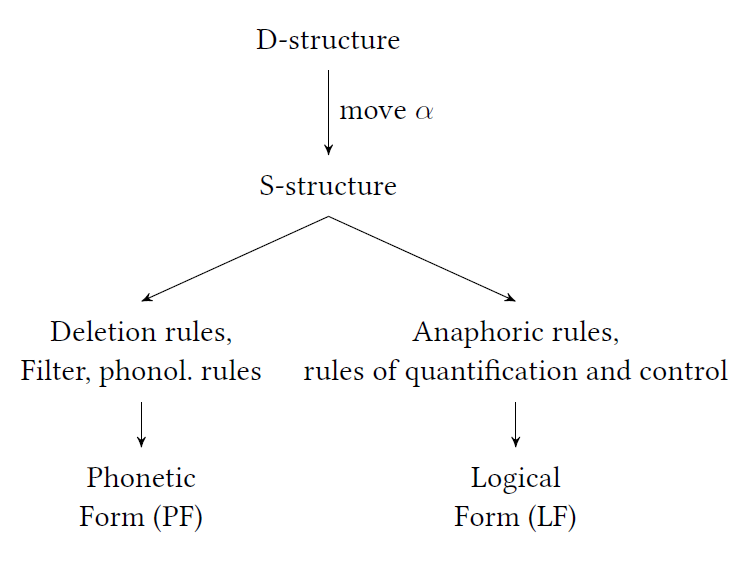
\includegraphics[scale=.43]{material/11tmodell}
%%	\caption{T-Modell \citep[vgl.][]{MuellerS15b}}
%%\end{figure}
%%	
%%\end{frame}
%
%\begin{frame}
%%\frametitle{T-Modell}
%
%\begin{figure}
%%\begin{tikzpicture}
%%\node at (0,0) {D-structure};
%%\draw[->] (0,-0.3)--(0,-1.5);
%%\node[right] at (0,-0.9) {move $\alpha$};
%%\node at (0,-1.8) {S-structure};
%%\draw[->] (0,-2.1)--(-1.5-3);
%%\draw[->] (0,-2.1)--(1.5,-3);
%%\end{tikzpicture}
%\begin{forest}
%	sm edges,
%	[D-structure, [S-structure,edge label={node[midway,right]{move $\alpha$} }
%		[{Deletion rules,}\\{Filter, phonol. rules} [Phonetic Form (PF)], align=center]
%		[{Anaphoric rules,}\\{rules of quantification and control}, align=center [Logical Form (LF)] ]
%	]]
%\end{forest}
%	\caption{T-Modell \citep[vgl.][]{MuellerS15b}}
%\end{figure}
%
%\end{frame}
%
%
%%%%%%%%%%%%%%%%%%%%%%%%%%%%%%%%%%%
%%%%%%%%%%%%%%%%%%%%%%%%%%%%%%%%%%%
%\subsection{Funktionale Phrasen II}
%
%\iftoggle{sectoc}{
%	\frame{
%		%\begin{multicols}{2}
%		\frametitle{~}
%		\tableofcontents[currentsubsection,subsubsectionstyle=hide]
%		%\end{multicols}
%	}
%}
%
%%%%%%%%%%%%%%%%%%%%%%%%%%%%%%%%%%%
%\begin{frame}
%\frametitle{Funktionale Phrasen II}
%
%\begin{itemize}
%	\item Bisher \ras Nebensatzstellung im Deutschen
%	\item Wann kommt die NS-Stellung vor? \ras Complementizer!
%	
%	\eal
%	\ex[]{(Ich denke,) \alertred{dass} Syntax Spaß machen sollte.}
%	\ex[]{Syntax \alertred{sollte} Spaß machen.}
%	\ex[]{(Ich frage mich,) \alertred{ob} der Winter jemals enden wird.}
%	\ex[]{Der Winter \alertred{wird} niemals enden.}
%	\ex[*]{Der Winter \alertred{ob wird} niemals enden.}
%	\zl
%	
%	\item Complementizer und finite Verben (in V2- und V1-Sätzen) sind \textbf{komplementär}!
%	
%\end{itemize}
%
%\end{frame}
%
%
%%%%%%%%%%%%%%%%%%%%%%%%%%%%%%%%%%%
%%%%%%%%%%%%%%%%%%%%%%%%%%%%%%%%%%%
%\subsubsection{Complementizer Phrase}
%%\frame{
%%\frametitle{~}
%%	\tableofcontents[currentsection]
%%}
%
%%%%%%%%%%%%%%%%%%%%%%%%%%%%%%%%%%%
%\begin{frame}
%\frametitle{Complementizer Phrase (CP)}
%
%\begin{itemize}
%	\item C nimmt eine IP als Komplement
%\end{itemize}
%
%\begin{minipage}[b]{0.45\textwidth}
%\begin{figure}
%	\centering
%	\scalebox{.6}{
%		\begin{forest}
%		sm edges,
%		[IP [DP [Peter,roof]]
%			[\MyPxbar{I} [VP 
%					[\MyPxbar{V} [DP [den Wagen,roof]]
%						[\zerobar{V} [gekauft]]
%						]]
%				[I [hat]]
%				]
%		]
%		\end{forest}
%		}
%		\caption{NS als IP}	
%\end{figure}		
%\end{minipage}  
%  	%  
%\pause
%	%
%\begin{minipage}[b]{0.45\textwidth}
%\begin{figure}
%	\centering
%	\scalebox{.6}{
%		\begin{forest}
%		sm edges,
%[CP	[\MyPxbar{C}	[\zerobar{C} [\alertred{dass}\\ \alertred{ob}\\ \alertred{weil}]]	
%		[IP [DP [Peter,roof]]
%			[\MyPxbar{I} [VP
%					[\MyPxbar{V} [DP [den Wagen,roof]]
%						[\zerobar{V} [gekauft]]
%						]]
%				[\zerobar{I} [\alertgreen{hat}]]
%				]
%		]
%	]
%]
%		\end{forest}
%		}
%		\caption{NS als CP}	
%\end{figure}		
%\end{minipage}  
%
%\nocite{Fries&MyP16i}
%
%\end{frame}
%
%
%%%%%%%%%%%%%%%%%%%%%%%%%%%%%%%%%%%
%\begin{frame}
%\frametitle{Complementizer Phrase}
%
%\begin{itemize}
%	\item Die CP ist für den Satzmodus zuständig.
%	\begin{itemize}
%		\item Eingebetteter Satz
%		\item Eingebetteter Fragesatz
%		\item Deklarativsatz
%		\item E- oder K-Fragesatz
%		\item Imperativsatz
%	\end{itemize}
%\end{itemize}
%\end{frame}
%
%
%%%%%%%%%%%%%%%%%%%%%%%%%%%%%%%%%%%
%\begin{frame}
%%\frametitle{Complementizer Phrase}
%
%\begin{itemize}
%	\item Die CP bestimmt die \textbf{Form} der IP. \ras Finit
%\end{itemize}
%
%\begin{figure}[b]
%
%	\begin{minipage}[b]{0.45\textwidth}
%	\centering
%	\tiny{
%		\begin{forest}
%		sm edges,
%[*CP	[\MyPxbar{C}	[\zerobar{C} [dass]]
%		[IP [DP [Peter,roof]]
%			[\MyPxbar{I} [VP 
%					[\MyPxbar{V} [DP [den Wagen,roof]]
%						[\zerobar{V} [\alertgreen{kaufen}]]{\draw[<-,HUred] (.south east)--++(0em,-1.5ex)--++(+3em,0pt)
%node[anchor=west,align=center]{infinit};}
%						]]
%				[\zerobar{I} [$\emptyset$]]
%				]
%		]
%	]
%]		
%		\end{forest}
%		}
%		\caption{Ungrammatisch}	
%  	\end{minipage}  
%  	%  
%	%
%	\begin{minipage}[b]{0.45\textwidth}
%	\centering
%	\tiny{
%		\begin{forest}
%		sm edges,
%[CP	[\MyPxbar{C}	[\zerobar{C} [dass]]	
%		[IP [DP [Peter,roof]]
%			[\MyPxbar{I} [VP 
%					[\MyPxbar{V} [DP [den Wagen,roof]]
%						[\zerobar{V} [t$_{i}$]]
%						]]
%				[\zerobar{I} [\alertgreen{kauft}$_{i}$]]{\draw[<-,HUred] (.south east)--++(0em,-1.5ex)--++(+2em,0pt)
%node[anchor=west,align=center]{finit};}
%				]
%		]
%	]
%]
%		\end{forest}
%		}
%		\caption{Grammatisch}	
%  	\end{minipage}  
%
%\end{figure}
%
%\end{frame}
%
%
%%%%%%%%%%%%%%%%%%%%%%%%%%%%%%%%%%%
%\begin{frame}
%%\frametitle{Complementizer Phrase}
%
%\begin{itemize}
%	\item Korrelation zwischen \textbf{Verbzweit- und Verbletztstruktur}
%	\item Kopfbewegung
%\end{itemize}
%
%
%\begin{minipage}[b]{0.49\textwidth}
%\begin{figure}
%	\centering
%	\tiny{
%		\begin{forest}
%		sm edges,
%[CP	[\MyPxbar{C}	[\zerobar{C} [\alertgreen{dass}]]{\draw[<-,HUred] (.south west)--++(0em,-2.5ex)--++(-1.5em,0pt)
%node[anchor=east,align=center]{besetzt! \ras \\ keine I-C-Bewegung};}
%		[IP [DP [Peter,roof]]
%			[\MyPxbar{I} [VP 
%					[\MyPxbar{V} [DP [den Wagen,roof]]
%						[\zerobar{V} [t$_{i}$]]
%						]]
%				[\zerobar{I} [\alertgreen{kauft$_{i}$}]]
%				]
%		]
%	]
%]		
%		\end{forest}
%		}
%		\caption{V-I-Bewegung}	
%\end{figure}		
%\end{minipage}  
%%  
%%
%\begin{minipage}[b]{0.49\textwidth}
%\begin{figure}
%	\centering
%	\tiny{
%		\begin{forest}
%		sm edges,
%[CP	[\MyPxbar{C}	[\zerobar{C} [\alertgreen{kauft$_{i}$}]]{\draw[<-,HUred] (.south west)--++(0em,-2.5ex)--++(-1.5em,0pt)
%node[anchor=east,align=center]{frei! \ras \\ I-C-Bewegung};}
%		[IP [DP [Peter,roof]]
%			[\MyPxbar{I} [VP 
%					[\MyPxbar{V} [DP [den Wagen,roof]]
%						[\zerobar{V} [t$_{i}$]]
%						]]
%				[\zerobar{I} [\alertgreen{t$_{i}$}]]
%				]
%		]
%	]
%]
%		\end{forest}
%		}
%		\caption{V-I-C-Bewegung}
%\end{figure}			
%\end{minipage}  
%
%\end{frame}
%
%
%%%%%%%%%%%%%%%%%%%%%%%%%%%%%%%%%%%
%\begin{frame}
%
%\begin{itemize}
%	\item \textbf{Weitere Position} für Verbzweitsätze \ras aber \textbf{nur eine} Phrasenposition
%\ea[*]{[Den Wagen] [Peter] kauft gestern.}
%\z
%
%\end{itemize}
%
%\begin{figure}[b]
%
%	\begin{minipage}[b]{0.49\textwidth}
%	\centering
%	\scalebox{.55}{
%		\begin{forest}
%		sm edges,
%[CP	[\alertgreen{DP$_{i}$} [Peter,roof]]{\draw[<-,HUred] (.south west)--++(0em,-1.5ex)--++(-2em,0pt)
%node[anchor=east,align=center]{Phrase};}
%	[\MyPxbar{C} [\zerobar{C} [kauft$_{ii}$]]
%		[IP 
%			[,empty nodes [\alertgreen{t$_{i}$}]]
%			[\MyPxbar{I} [VP 
%					[\MyPxbar{V} [DP [den Wagen,roof]]
%						[\zerobar{V} [t$_{ii}$]]
%						]]
%				[\zerobar{I} [t$_{ii}$]]
%				]
%		]
%	]
%]		
%		\end{forest}
%		}
%		\caption{Subjektbewegung}	
%  	\end{minipage}  
%%%
%\pause
%%%
%	\begin{minipage}[b]{0.49\textwidth}
%	\centering
%	\scalebox{.55}{
%		\begin{forest}
%		sm edges,
%[CP	[\alertgreen{DP$_{ii}$} [den Wagen,roof]]{\draw[<-,HUred] (.south west)--++(0em,-1.5ex)--++(-2em,0pt)
%node[anchor=east,align=center]{Phrase};}
%	[\MyPxbar{C}	[\zerobar{C} [kauft$_{i}$]]
%		[IP [DP [Peter,roof]]
%			[\MyPxbar{I} [VP 
%					[\MyPxbar{V} 
%						[,empty nodes [\alertgreen{t$_{ii}$}]]
%						[\zerobar{V} [t$_{i}$]]
%						]]
%				[\zerobar{I} [t$_{i}$]]
%				]
%		]
%	]
%]
%		\end{forest}
%		}
%		\caption{Objektbewegung}	
%  	\end{minipage}  
%    
%\end{figure}
%
%\end{frame}
%
%
%%%%%%%%%%%%%%%%%%%%%%%%%%%%%%%%%%%
%\begin{frame}
%\frametitle{Complementizer Phrase}
%
%\begin{itemize}
%	\item Die CP ist für den \textbf{Satzmodus} und die \textbf{illokutionäre Kraft} zuständig.
%\end{itemize}
%
%\begin{figure}[b]
%
%	\begin{minipage}[b]{0.45\textwidth}
%	\centering
%	\scriptsize{
%		\begin{forest}
%		MyP edges,
%		[CP [$\emptyset$]{\draw[<-,HUred] (.south west)--++(0em,-1.5ex)--++(-2em,0pt)
%node[anchor=east,align=center]{leer};}
%			[C' [C [dass]]{\draw[<-,HUred] (.south west)--++(0em,-1.5ex)--++(-2em,0pt)
%node[anchor=east,align=center]{Subjunktion};}
%				[IP [Peter den Wagen kauft,roof]]]]
%		\end{forest}
%		}
%		\caption{Eingebetteter Satz}	
%  	\end{minipage}  
%%  
%\pause            
%%         
%  	\begin{minipage}[b]{0.45\textwidth}
%	\centering
%	\scriptsize{
%		\begin{forest}
%		MyP edges,
%		[CP [$\emptyset$]{\draw[<-,HUred] (.south west)--++(0em,-1.5ex)--++(-2em,0pt)
%node[anchor=east,align=center]{leer};}
%			[C' [C [kauft$_{i}$]]{\draw[<-,HUred] (.south west)--++(0em,-1.5ex)--++(-2em,0pt)
%node[anchor=east,align=center]{Verb};}
%				[IP [Peter den Wagen t$_{i}$,roof]]]]
%		\end{forest}
%		}
%		\caption{Entscheidungsfrage}
%  	\end{minipage}  
%  	
%\end{figure}
%
%\end{frame}
%
%
%%%%%%%%%%%%%%%%%%%%%%%%%%%%%%%%%%%
%\begin{frame}
%\frametitle{Complementizer Phrase}
%
%\begin{itemize}
%	\item Die CP ist für den \textbf{Satzmodus} und die \textbf{illokutionäre Kraft} zuständig.
%\end{itemize}
%
%\begin{figure}[b]
%
%	\begin{minipage}[b]{0.45\textwidth}
%	\centering
%	\scriptsize{
%		\begin{forest}
%		MyP edges,
%		[CP [DP$_{ii}$ [was,roof]]{\draw[<-,HUred] (.south west)--++(0em,-1.5ex)--++(-2em,0pt)
%node[anchor=east,align=center]{W-Wort};}
%			[C' [C [kauft$_{i}$]]{\draw[<-,HUred] (.south west)--++(0em,-1.5ex)--++(-2em,0pt)
%node[anchor=east,align=center]{Verb};}
%				[IP [Peter t$_{ii}$ t$_{i}$,roof]]]]
%		\end{forest}
%		}
%		\caption{Konstituentenfrage}	
%  	\end{minipage}  
%  	%  
%  	\pause            
%  	%         
%  	\begin{minipage}[b]{0.49\textwidth}
%	\centering
%	\scriptsize{
%		\begin{forest}
%		MyP edges,
%		[CP [DP$_{ii}$ [Den Wagen,roof]]{\draw[<-,HUred] (.south west)--++(0em,-1.5ex)--++(-2em,0pt)
%node[anchor=east,align=center]{Konstituente};}
%			[C' [C [kauft$_{i}$]]{\draw[<-,HUred] (.south west)--++(0em,-1.5ex)--++(-2em,0pt)
%node[anchor=east,align=center]{Verb};}
%				[IP [Peter t$_{ii}$ t$_{i}$,roof]]]]
%		\end{forest}
%		}
%		\caption{Aussagesatz}
%  	\end{minipage}  
%  
%\end{figure}
%
%\end{frame}
%
%
%%%%%%%%%%%%%%%%%%%%%%%%%%%%%%%%%%%
%%%%%%%%%%%%%%%%%%%%%%%%%%%%%%%%%%%
%\subsection{Erklärungspotential}
%
%\iftoggle{sectoc}{
%	\frame{
%		%\begin{multicols}{2}
%		\frametitle{~}
%		\tableofcontents[currentsubsection,subsubsectionstyle=hide]
%		%\end{multicols}
%	}
%}
%
%%%%%%%%%%%%%%%%%%%%%%%%%%%%%%%%%%%%
%\begin{frame}
%\frametitle{Erklärungspotential}
%
%\begin{itemize}
%	\item Warum ist eine \textbf{VP mit Subjekt} nicht möglich?
%	\eal 
%	\ex[]{\dots\ (dass) [Peter den Wagen \alertred{kauft}]$_{IP}$.}
%	\ex[*]{\dots\ (dass) [Peter den Wagen \alertred{kaufen}]$_{VP}$.}
%	\zl
%
%\pause
%	\begin{itemize}
%		\item \textbf{Kasus} und \textbf{$\theta$-Rolle} werden \textbf{strukturell} vergeben.
%		\item[]
%		\item Erst durch die \textbf{Subjekt-Verb-Kongruenz} erhält das Subjekt \textsc{nom}-Kasus.
%		\item[]
%		\item Subjekt-Verb-Kongruenz geschieht durch die \textbf{SpecIP-I$^{0}$-Relation} (strukturelle/lokale Relation).
%	\end{itemize}
%\end{itemize}		
%
%\end{frame}
%
%
%%%%%%%%%%%%%%%%%%%%%%%%%%%%%%%%%%%%
%\begin{frame}
%
%\begin{itemize}
%	\item Warum ist eine \textbf{VP mit Subjekt} nicht möglich?
%	\eal 
%	\ex[]{\dots\ (dass) [Peter den Wagen \alertred{kauft}]$_{IP}$.}
%	\ex[*]{\dots\ (dass) [Peter den Wagen \alertred{kaufen}]$_{VP}$.}
%	\zl
%
%\end{itemize}
%
%\begin{figure}[b]
%%	\begin{minipage}[b]{0.80\textwidth}
%	\centering
%	\scriptsize{
%		\begin{forest}
%		MyP edges,
%		[IP 
%			[DP [Peter,roof]]{\draw[<-,HUred] (.north west)--++(0em,+1.5ex)--++(-2em,0pt)
%node[anchor=east,align=center]{\textsc{agens}- \& \\ \textsc{akk}-Vergabe};}
%			[\MyPxbar{I} 
%				[VP 					
%					[\MyPxbar{V} 
%						[DP [den Wagen,roof]]{\draw[<-,HUred] (.north west)--++(0em,+1.5ex)--++(-2em,0pt)
%node[anchor=east,align=center]{\textsc{patiens}- \& \\ \textsc{akk}-Vergabe};}
%						[\zerobar{V} [gekauft]]
%					]
%				]
%				[\zerobar{I} [hat]]
%			]
%		]
%		\end{forest}
%		}
%	\caption{Position und Funktion im X-Bar-Schema} 
%%  	\end{minipage}  
% 
%\end{figure}
%
%\end{frame}
%
%
%%%%%%%%%%%%%%%%%%%%%%%%%%%%%%%%%%%%
%\begin{frame}
%\frametitle{Erklärungspotential}
%
%
%\begin{itemize}
%	\item Warum ist die \textbf{Vorfeldbesetzung durch VP mit Subjekt} nicht möglich?
%	\eal 
%	\ex[]{[Den Wagen \alertred{gekauft}]$_{VP}$ hat Peter gestern.}
%	\ex[*]{[Peter den Wagen \alertred{gekauft}]$_{VP}$ hat gestern.}
%	\zl
%
%\pause
%	\item Damit das Subjekt sichtbar (overt realisiert) wird, muss es \textbf{in SpecIP} \textsc{nom} \textbf{erhalten} \ras Es ist nicht (mehr) in der VP!
%
%\end{itemize}		
%
%\pause
%\begin{itemize}
%	\item \textbf{Gewinn} \ras Elegante und restriktive Theorie \nocite{Haspelmath94a}
%
%	\begin{itemize}
%		\item Keine \textbf{Köpfe} ohne Phrasen
%		\item Keine \textbf{Phrasen} ohne Köpfe (exozentrische Phrasen)
%		\item Strukturelle \textbf{Position} bestimmt Funktion
%		\item \textbf{Einheitlichkeit} der X-Bar-Struktur
%	\end{itemize}		
%
%\end{itemize}
%
%\end{frame}
%
%
%%%%%%%%%%%%%%%%%%%%%%%%%%%%%%%%%%%%
%\begin{frame}
%
%\begin{itemize}
%	\item \textbf{Grammatikalisierung} \ras ein seltenes Argument \citep{Haspelmath94a}
%	\item Hilfsverben, Tempus- und Aspektaffixe werden \textbf{aus Vollverben} grammatikalisiert \ras \textbf{Unterschied zwischen Wort oder Affix} ist nicht von Bedeutung.
%	\item Die \textbf{Kopf-Dependent-Relation} bleibt bei der Grammatikalisierung immer erhalten \ras Hilfsverben und weitere Affixe sind Köpfe.
%\end{itemize}
%
%
%\begin{figure}[b]
%
%	\begin{minipage}[b]{0.40\textwidth}
%	\centering
%	\scalebox{.8}{
%		\begin{forest}
%		MyP edges,
%		[VP [DP [Julia,roof]]
%			[\MyPxbar{V} [VP [cantare,roof]]
%				[\zerobar{V} [\alertgreen{habet}]]		{\draw[<-,HUred] (.south east)--++(0em,-1.5ex)--++(+2em,0pt)
%node[anchor=west,align=center]{Kopf};}
%			]
%		]
%		\end{forest}
%		}
%		\caption{Latein}	
%  	\end{minipage}  
%  	%  
%  	\pause            
%  	%         
%  	\begin{minipage}[b]{0.40\textwidth}
%	\centering
%	\scalebox{.8}{
%		\begin{forest}
%		MyP edges,
%		[IP [DP [Julia,roof]]
%			[\MyPxbar{I} [VP [cant-,roof]]
%				[\zerobar{I} [\alertgreen{-ará}]]{\draw[<-,HUred] (.south east)--++(0em,-1.5ex)--++(+2em,0pt)
%node[anchor=west,align=center]{Kopf};}
%			]
%		]
%		\end{forest}
%		}
%		\caption{Spanisch}
%  	\end{minipage}  
%  	
%\end{figure}
%
%
%\end{frame}
%
%
%%%%%%%%%%%%%%%%%%%%%%%%%%%%%%%%%%%
%%%%%%%%%%%%%%%%%%%%%%%%%%%%%%%%%%%
%\subsection{Mehr funktionale Kategorien}
%
%\iftoggle{sectoc}{
%	\frame{
%		%\begin{multicols}{2}
%		\frametitle{~}
%		\tableofcontents[currentsubsection,subsubsectionstyle=hide]
%		%\end{multicols}
%	}
%}
%
%
%%%%%%%%%%%%%%%%%%%%%%%%%%%%%%%%%%%%
%%\begin{frame}
%%\frametitle{Mehr funktionale Kategorien}
%%\nocite{Lenerz93a}
%%
%%\begin{figure}[b]
%%	\begin{minipage}[b]{0.48\textwidth}
%%		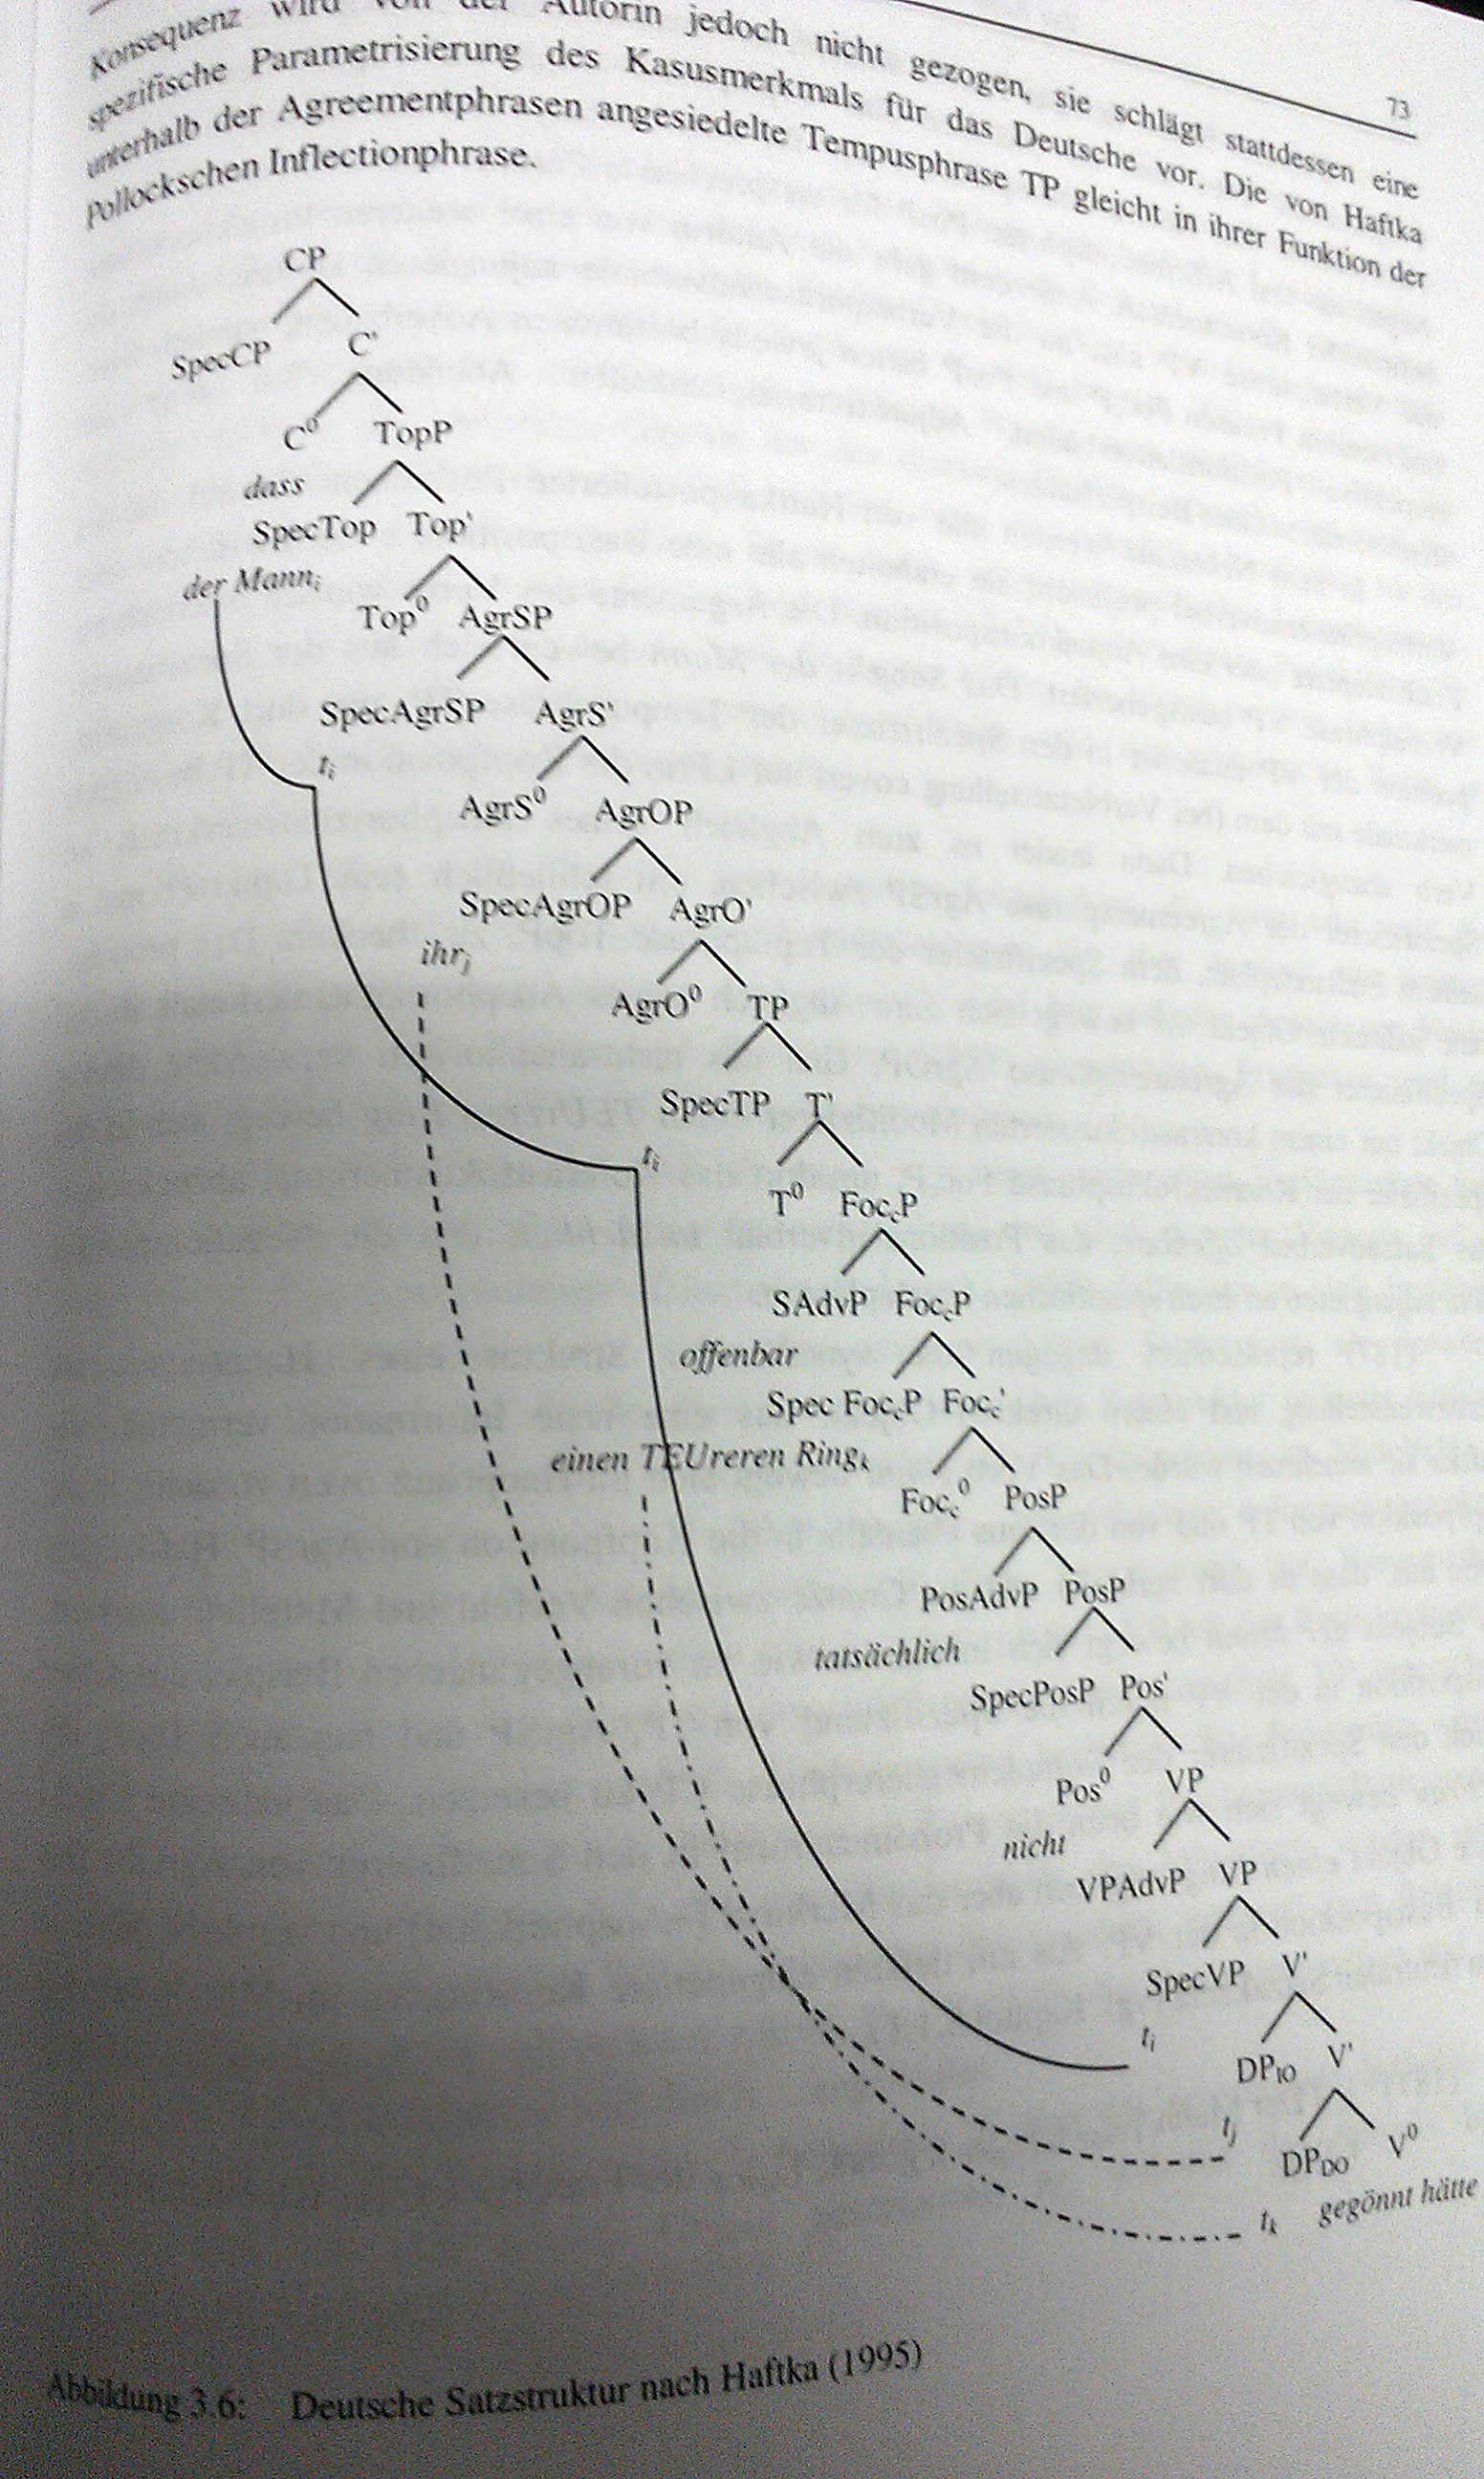
\includegraphics[scale=0.06]{material/Haftka95CP}
%%		\caption{CP-Struktur (Haftka 1995)}
%%		%\label{Zeichen1}
%%	\end{minipage}
%%	%
%%	%				
%%	\begin{minipage}[b]{0.48\textwidth}
%%		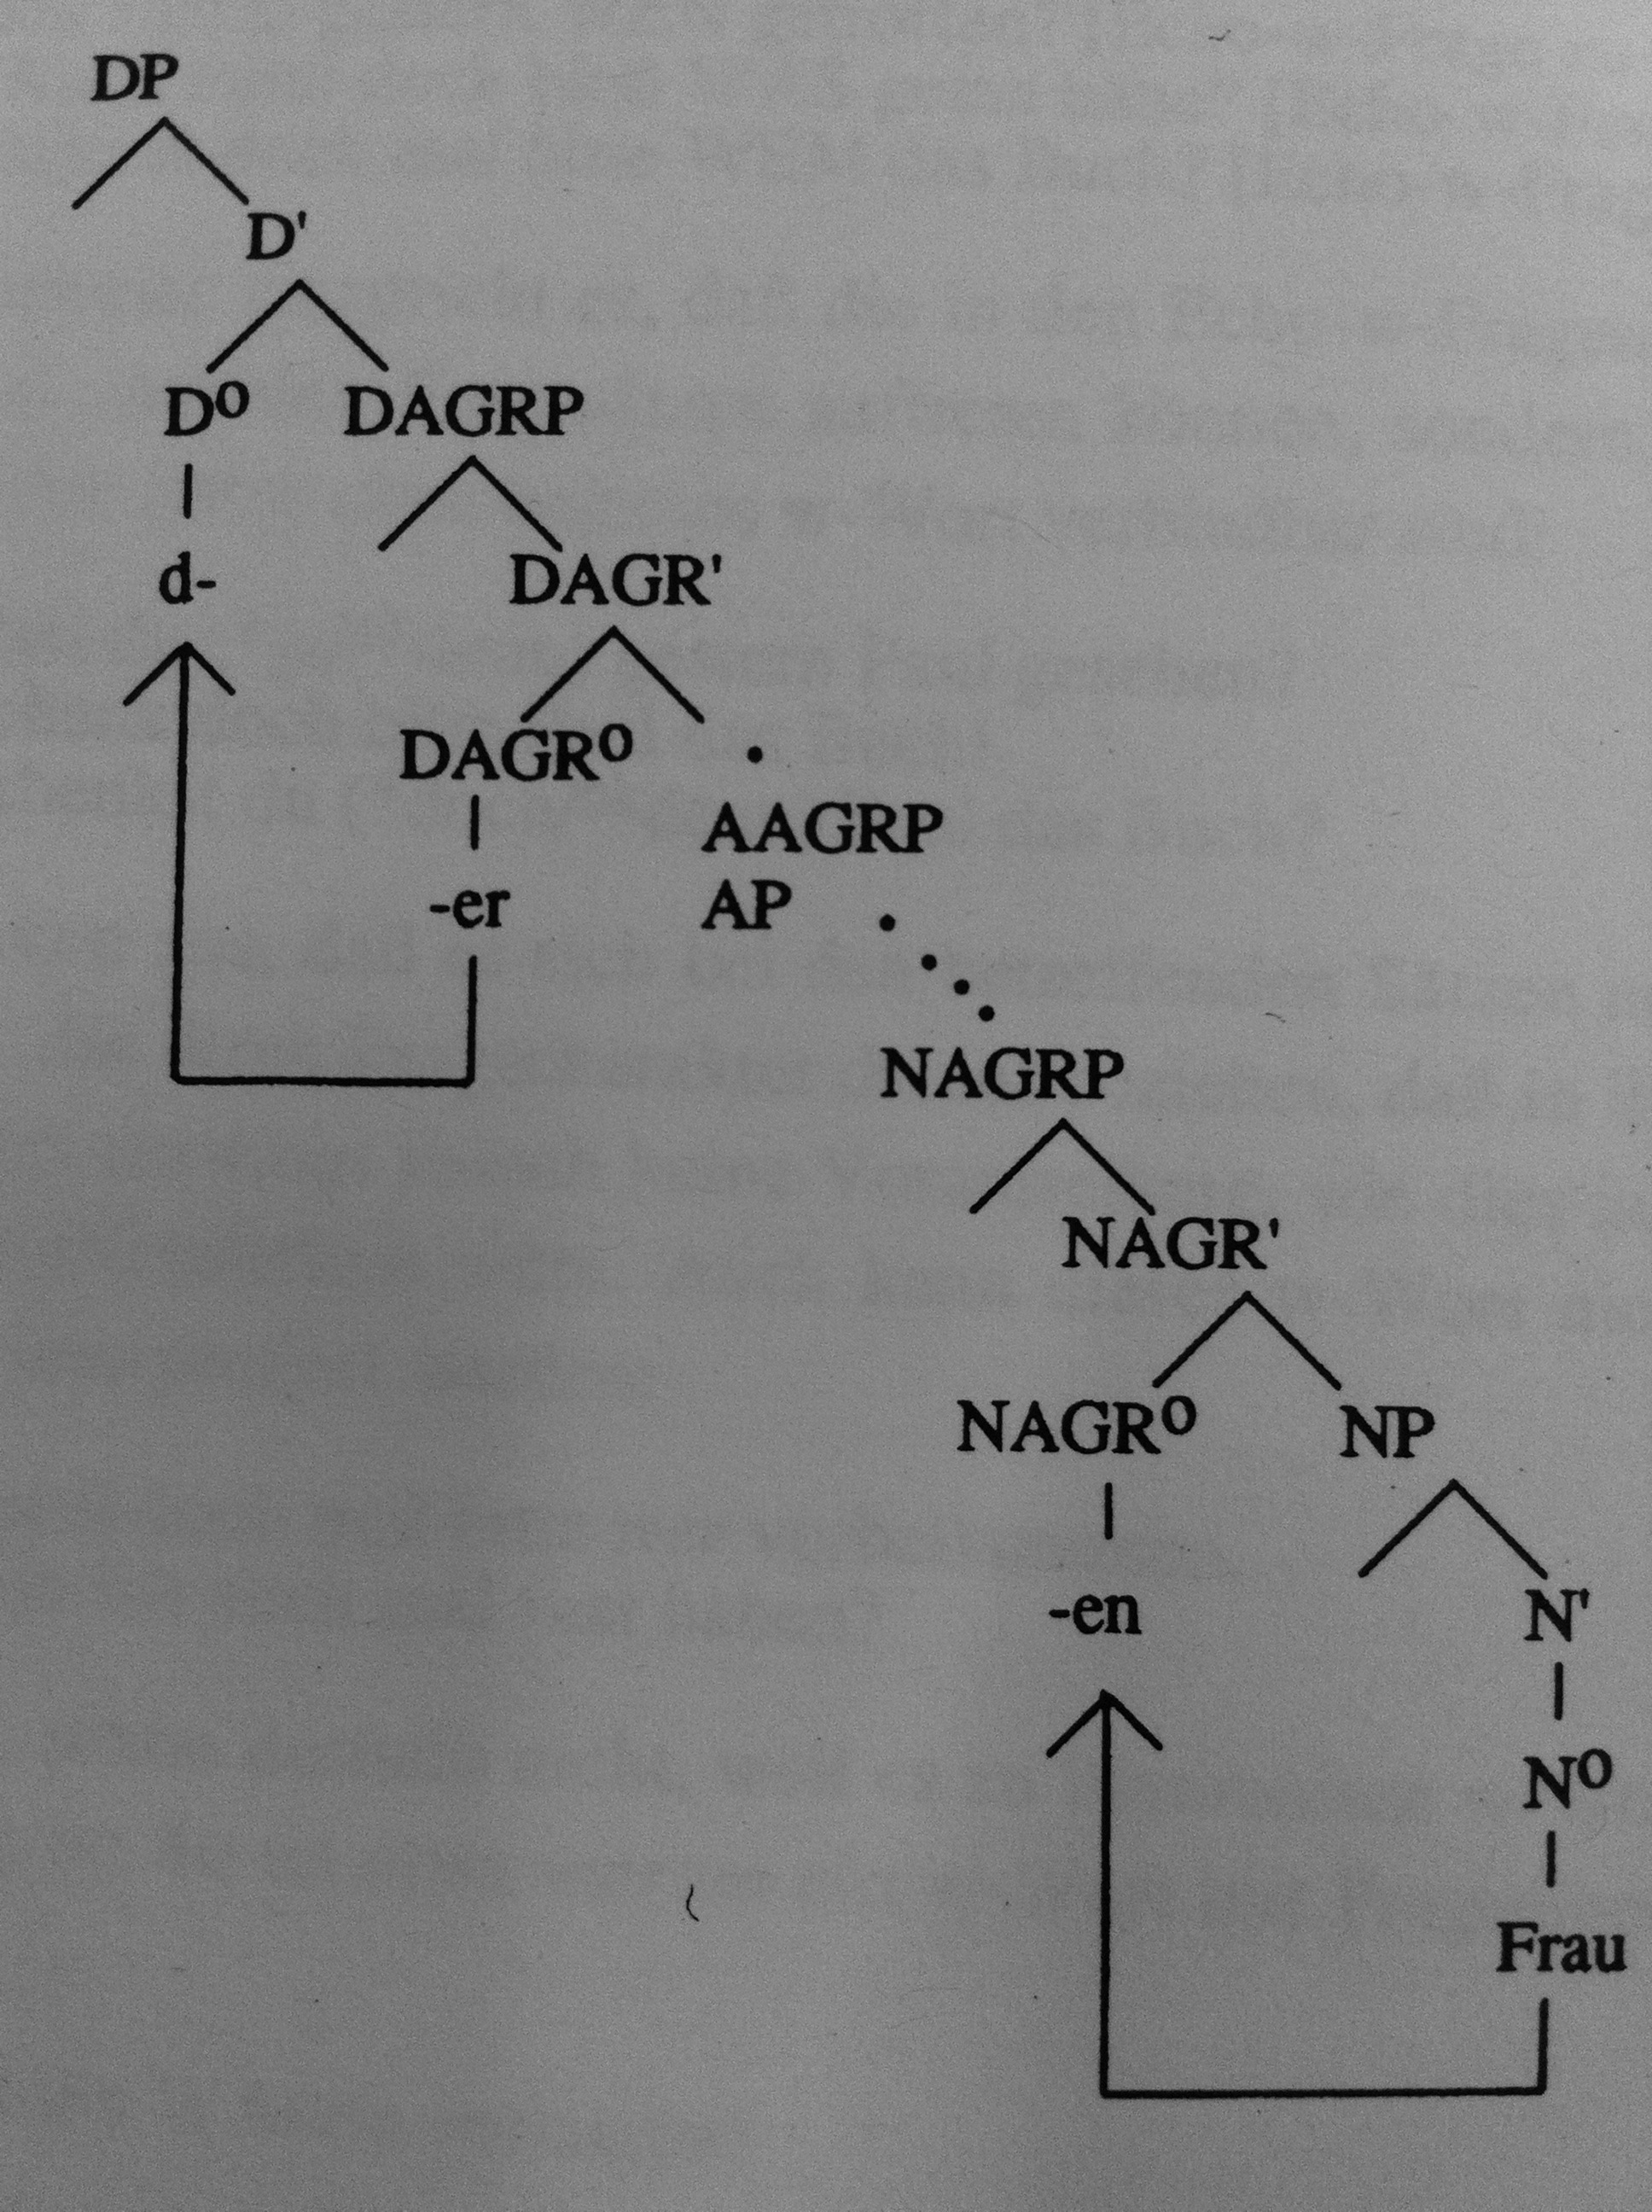
\includegraphics[scale=0.06]{material/Lenerz93DP}
%%		\caption{DP-Struktur \citep{Lenerz93a}}
%%		%\label{Zeichen2}
%%	\end{minipage}                        
%%\end{figure}
%%
%%\end{frame}
%
%
%\begin{frame}
%\nocite{Lenerz93a}
%
%	\begin{minipage}[c]{0.48\textwidth}
%\begin{figure}
%	\centering
%	\scalebox{.45}{\begin{forest}MyP edges,
%			[DP
%			[]
%			[D'
%				[\zerobar{D} [d-, name=d] ]
%				[DAGRP
%					[]
%					[DAGRP'
%						[\zerobar{DAGRP} [-er, name=er] ]
%						[{AAGRP}\\{AP}, align=center [NAGRP, edge=dotted
%						[]
%						[NAGR'
%							[\zerobar{NAGR} [-en, name=en] ]
%							[NP
%								[]
%								[N' [\zerobar{N} [Frau, name=Frau] ] ]
%							]
%						]
%						] ]
%					]
%			]
%			] ]{
%			\draw[->] (Frau) to [out=south west, in=south] (en.south);
%			\draw[->] (er) to [out=south west, in=south] (d.south);}
%		\end{forest}}
%	\caption{DP-Struktur \citep{Lenerz93a}}
%\end{figure}
%	\end{minipage}
%	%
%	%				
%	\begin{minipage}[c]{0.48\textwidth}
%\begin{figure}
%			\centering 
%			\scalebox{.19}{	\begin{forest}
%				[CP
%					[SpecCP]
%					[C'
%						[{\zerobar{C}}\\{dass}, align=center]
%						[TopP
%							[SpecTop \\ \textit{der Mann\textsubscript{i}}, align=center, name=Mann]
%							[Top'
%								[\zerobar{Top}]
%								[AgrSP
%									[SpecAgrSP \\ t\textsubscript{i}, align=center, name=Agr]
%									[AgrS'
%										[\zerobar{AgrS}]
%										[AgrOP
%											[SpecAgrOP \\ \textit{ihr\textsubscript{j}}, align=center, name=ihr]
%											[AgrO'
%												[\zerobar{AgrO}]
%												[TP
%													[SpecTP \\ t\textsubscript{i}, align=center, name=i1]
%													[T'
%														[\zerobar{T}]
%														[Foc\textsubscript{c}P
%															[SAdvP\\ \textit{offenbar}, align=center]
%															[Foc\textsubscript{c}P
%															[SpecFoc\textsubscript{c}P \\ \textit{einen TEUeren Ring\textsubscript{k}}, align=center, name=ring]
%															[Foc\textsubscript{c}'
%																[\zerobar{Foc\textsubscript{c}}]
%																[PosP
%																	[PosAdvP \\ \textit{tatsächlich}, align=center]
%																	[PosP
%																		[SpecPosP]
%																		[Pos'
%																			[\zerobar{Pos}\\nicht, align=center]
%																			[VP	
%																				[VPAdvP]
%																				[VP
%																					[SpecVP\\ t\textsubscript{i}, align=center, name=i2]
%																					[V'
%																						[DP\textsubscript{IO} \\ t\textsubscript{j}, align=center, name=j]
%																						[V'
%																							[DP\textsubscript{DO} \\ t\textsubscript{k}, align=center, name=k]
%																							[\zerobar{V}\\\textit{gegönnt hätte}, align=center]
%																						]
%																					]
%																				]
%																			]
%																		]
%																	]
%																]
%																]
%															]	
%															]
%														]
%													]			
%												]
%											]
%										]
%									]
%								]
%							]
%						]
%					]
%					{\draw (i2) to [out=south west, in=south] (i1) to [out=south west, in=south] (Agr) to [out=south west, in=south] (Mann);
%				\draw[dashed, thick] (j) to [out=south west, in=south] (ihr);
%					\draw[dotted, thick] (k) to [out=south west, in=south] (ring);
%				}
%			\end{forest}}
%		\caption{CP-Struktur (Haftka 1995)}
%		\end{figure}
%	\end{minipage}                        
%
%\end{frame}
%
%%%%%%%%%%%%%%%%%%%%%%%%%%%%%%%%%%%
%%%%%%%%%%%%%%%%%%%%%%%%%%%%%%%%%%%
%\subsection{Übung}
%
%\iftoggle{sectoc}{
%	\frame{
%		%\begin{multicols}{2}
%		\frametitle{~}
%		\tableofcontents[currentsubsection,subsubsectionstyle=hide]
%		%\end{multicols}
%	}
%}
%
%
%%%%%%%%%%%%%%%%%%%%%%%%%%%%%%%%%%%%
%%%%%%%%%%%%%%%%%%%%%%%%%%%%%%%%%%%%
%
%%%%%%%%%%%%%%%%%%%%%%%%%%%%%%%%%%%%
%\begin{frame}
%\frametitle{Übung}
%
%\begin{itemize}
%		\item Erklären Sie mithilfe des X-Bar-Schemas die \textbf{Ambiguität} im folgenden Satz:
%	
%		\ea Das Kind küsst die Mama.
%		\z
%
%\end{itemize}
%\end{frame}
%
%
%%%%%%%%%%%%%%%%%%%%%%%%%%%%%%%%%%%%
%
%\iftoggle{ue-loesung}{
%
%\input{loesungen/06f-ue-loesung01-include}
%
%}
%
%%%%%%%%%%%%%%%%%%%%%%%%%%%%%%%%%%%%
%
%\begin{frame}
%\frametitle{Übung}
%
%\begin{itemize}
%
%	\item Erklären Sie mithilfe des X-Bar-Schemas, warum der folgende Satz \textbf{ungrammatisch} ist:
%	
%	\ea Im Auto ich habe heute geschlafen.
%	\z
%	
%\end{itemize}
%\end{frame}
%
%
%
%%%%%%%%%%%%%%%%%%%%%%%%%%%%%%%%%%%%
%
%\iftoggle{ue-loesung}{
%
%\input{loesungen/06f-ue-loesung02-include}
%}
%
%%%%%%%%%%%%%%%%%%%%%%%%%%%%%%%%%%%%
%
%%%%%%%%%%%%%%%%%%%%%%%%%%%%%%%%%%%%
%\begin{frame}
%\frametitle{Übung}
%
%\begin{itemize}
%	\item Was ist an dieser Struktur misslungen? Beziehen Sie sich in Ihrer Antwort \ua auf die in der Sitzung behandelten Köpfigkeitsmerkmale und Strukturaufbaugesetzmäßigkeiten.
%\end{itemize}
%
%\begin{figure}
%\scalebox{.75}{\begin{forest} sm edges,
%		[S
%			[VP [V [Tea] ] ]
%			[NP
%				[P [with]]
%				[Det [some]]
%				[N [lemon]]
%			]
%			[PP
%				[P [tastes]]
%				[NP [Adj [really] ] [N [nice]] ]
%			]
%		]
%	\end{forest}}
%%	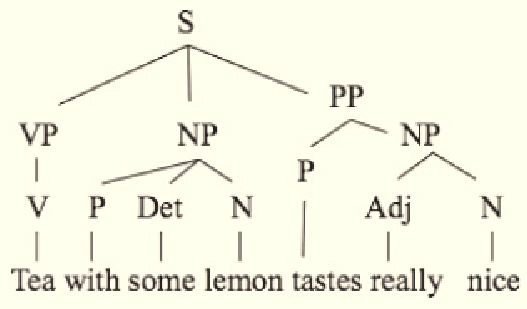
\includegraphics[scale=.45]{material/wrongtree}
%	\caption{vgl.\ \url{http://specgram.com/CLXV.1/05.cruz-ferreira.know22.html}}
%\end{figure}
%	
%\end{frame}
%
%
%
%%%%%%%%%%%%%%%%%%%%%%%%%%%%%%%%%%%%
%
%\iftoggle{ue-loesung}{
%	
%\input{loesungen/06f-ue-loesung03-include}
%
%}
%
%
%%%%%%%%%%%%%%%%%%%%%%%%%%%%%%%%%%%
%%%%%%%%%%%%%%%%%%%%%%%%%%%%%%%%%%%
%
%\subsection{Hausaufgabe}
%
%%%%%%%%%%%%%%%%%%%%%%%%%%%%%%%%%%%%
%%%%%%%%%%%%%%%%%%%%%%%%%%%%%%%%%%%%
%
%%%%%%%%%%%%%%%%%%%%%%%%%%%%%%%%%%%
%\begin{frame}
%\frametitle{Hausaufgabe}
%
%\begin{itemize}
%	\item Geben Sie an, um welchen \textbf{Phrasentyp} es sich bei den folgenden Phrasen handelt, und \textbf{welches Wort} sich in der \textbf{Kopfposition} der Phrasen befindet.
%	
%	\eal
%	\ex viele besorgte Mütter
%	\ex den Menschen in Not helfen
%	\ex Wasser ohne Kohlensäure
%	\ex auf Maria warten
%	\ex ob sie heute kommen werden
%	\ex Peter seine Traumfrau gefunden hat
%	\zl
%	
%\end{itemize}
%
%\end{frame}
%
%%%%%%%%%%%%%%%%%%%%%%%%%%%%%%%%%%%%
%
%%%%%%%%%%%%%%%%%%%%%%%%%%%%%%%%%%%
%\begin{frame}
%\frametitle{Hausaufgabe}
%
%\begin{itemize}
%	\item Analysieren Sie die folgenden Phrasen nach dem X-Bar-Schema (ohne Abkürzungen).
%
%	\ea Peter schläft.
%	\ex Wer schläft?
%	\ex Hat sie dir die schwierige Frage nach den Spuren gestellt?
%	\ex die fast vor dem Mittagessen erstellte Speisekarte
%	\ex weil der Präsident kommt, hat die Polizei die Sicherung des Geländes übernommen
%	\z
%
%\end{itemize}
%\end{frame}
%
%
%%%%%%%%%%%%%%%%%%%%%%%%%%%%%%%%%%%%%%%%%%%%%
%
%\iftoggle{ha-loesung}{
%
%\input{loesungen/06f-ha-loesung-include}
%
%}
%
%
%
%%%%%%%%%%%%%%%%%%%%%%%%%%%%%%%%%%%%
%%%%%%%%%%%%%%%%%%%%%%%%%%%%%%%%%%%%
%\begin{frame}
%\frametitle{Schluss!}
%
%\begin{figure}
%	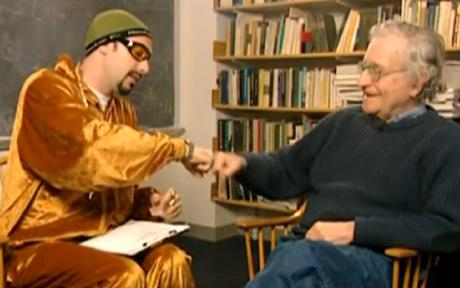
\includegraphics[scale=.5]{material/11chomksy}
%	\caption{Geschafft!}
%\end{figure}
%	
%\end{frame}

 %corrupted
%%%%%%%%%%%%%%%%%%%%%%%%%%%%%%%%%%%%%%%%%%%%%%%%
%% Compile the master file!
%% 		Slides: Antonio Machicao y Priemer
%% 		Course: GK Linguistik
%%%%%%%%%%%%%%%%%%%%%%%%%%%%%%%%%%%%%%%%%%%%%%%%


%%%%%%%%%%%%%%%%%%%%%%%%%%%%%%%%%%%%%%%%%%%%%%%%%%%%
%%%             Metadata                         
%%%%%%%%%%%%%%%%%%%%%%%%%%%%%%%%%%%%%%%%%%%%%%%%%%%%      

\title{Grundkurs Linguistik}

\subtitle{Syntax VII: X-Bar-Theorie - Funktionale Phrasen II}

\author[A. Machicao y Priemer]{
	{\small Antonio Machicao y Priemer}
	\\
	{\footnotesize \url{http://www.linguistik.hu-berlin.de/staff/amyp}}
%	\\
%	{\footnotesize \href{mailto:mapriema@hu-berlin.de}{mapriema@hu-berlin.de}}
}

\institute{Institut für deutsche Sprache und Linguistik}

\date{ }

%\publishers{\textbf{6. linguistischer Methodenworkshop \\ Humboldt-Universität zu Berlin}}

%\hyphenation{nobreak}


%%%%%%%%%%%%%%%%%%%%%%%%%%%%%%%%%%%%%%%%%%%%%%%%%%%%
%%%             Preamble's End                   %%%
%%%%%%%%%%%%%%%%%%%%%%%%%%%%%%%%%%%%%%%%%%%%%%%%%%%%      


%%%%%%%%%%%%%%%%%%%%%%%%%      
\huberlintitlepage[22pt]
\iftoggle{toc}{
\frame{
\begin{multicols}{2}
	\frametitle{Inhaltsverzeichnis}\tableofcontents
	%[pausesections]
\end{multicols}
	}
	}


%%%%%%%%%%%%%%%%%%%%%%%%%%%%%%%%%%
%%%%%%%%%%%%%%%%%%%%%%%%%%%%%%%%%%
%%%%%LITERATURE:

%\nocite{Altmann&Hofmann08a}
%\nocite{Altmann93a}
\nocite{Brandt&Co06a}
\nocite{Glueck05a} 
\nocite{Grewendorf&Co91a} 
\nocite{Luedeling2009a} 
%\nocite{Meibauer&Co07a}
\nocite{MuellerS13f} 
\nocite{MuellerS15b}
%% Allgemein
\nocite{Glueck&Roedel16a}
%\nocite{Meibauer&Co07a} 
\nocite{Repp&Co15a} 

%% Morphologie
%\nocite{Eisenberg04}

%% Syntax
\nocite{Adger04a}
%\nocite{Altmann&Hofmann08a} % Satztypen & Satzmodi
%\nocite{Altmann93a} % Satztypen & Satzmodi
\nocite{Brandt&Co06a} 
\nocite{Fanselow&Sascha87a}
\nocite{Fanselow&Sascha93a}
%\nocite{Fries&MyP16b} % Akzeptabilität
%\nocite{Fries16a} % Grammatikalität
%\nocite{Fries&MyP16d} % Kompetenz vs Performanz
\nocite{Fries&MyP16c} % GG
\nocite{Fries&MyP16a} % X-Bar-Theorie
%\nocite{Fries16e} % Satztyp
%\nocite{Fries16d} % Satzmodus 
\nocite{Grewendorf&Co91a} 
%\nocite{MyP17b} % Kerngrammatik
%\nocite{MyP18a} % Konstituententest
\nocite{MyP18b} % Kopf
\nocite{MyP18c} % Phrase
\nocite{MyP18s} % Funktionale Kategorie
\nocite{MyP18t} % Argumentstruktur
%\nocite{MuellerS13f} 
%\nocite{MuellerS15b}
\nocite{Stechow&Sternefeld88a}
\nocite{Sternefeld06a}
\nocite{Sternefeld06b}
%\nocite{Woellstein10a} % Topologisches Feldermodell
%%%%%%%%%%%%%%%%%%%%%%%%%%%%%%%%%

\begin{frame}
\frametitle{Begleitlektüre}

	\begin{itemize}
		\item \textbf{obligatorisch:}
			\begin{itemize}
				\item[] AM S.~86--94
				\item[] \cite{Luedeling2009a}: Kapitel 12 \& 13 (S.~142--158)
			\end{itemize}
	\end{itemize}

\end{frame}

%%%%%%%%%%%%%%%%%%%%%%%%%%%%%%%%%

%%%%%%%%%%%%%%%%%%%%%%%%%%%%%%%%%
\section{Syntax VII}
%%%%%%%%%%%%%%%%%%%%%%%%%%%%%%%%%

%%%%%%%%%%%%%%%%%%%%%%%%%%%%%%%%%%
\subsection{Move $\alpha$}

\iftoggle{sectoc}{
	\frame{
		%\begin{multicols}{2}
		\frametitle{~}
		\tableofcontents[currentsubsection,subsubsectionstyle=hide]
		%\end{multicols}
	}
}


%%%%%%%%%%%%%%%%%%%%%%%%%%%%%%%%%%
\begin{frame}
	\frametitle{Move $\alpha$}
	
	\begin{itemize}
		\item Lexikalische Einheiten werden aus dem Lexikon entnommen und in die \textbf{syntaktische Struktur} eingesetzt.
		\item[]
		\item Abhängig von der \textbf{Position}, die die lexikalischen Einheiten in der syntaktischen Struktur belegen, erfüllen sie eine \textbf{Funktion} (Position \ras Funktion).
	\end{itemize}
	
	\begin{block}{Basisposition}
		Syntaktische Position, an der eine Phrase basisgeneriert wird, d.\,h. an die sie in der syntaktischen Struktur eingefügt wird\\
		%Die Basisposition wird von der Struktur bestimmt und ist im Subkategorisierungsrahmen kodiert:\\
		%\textbf{schenken:}\\
		%DP$_{\textsc{nom,ag}}$ DP$_{\textsc{dat,ziel}}$  DP$_{\textsc{akk,th}}$ $\underline{\qquad}$ 
	\end{block}
	
	\nocite{Fries16h}
	
\end{frame}


%%%%%%%%%%%%%%%%%%%%%%%%%%%%%%%%%%
\begin{frame}
	
	\begin{itemize}
		\item Die Basisposition wird von der Struktur bestimmt und ist im Subkategorisierungsrahmen kodiert:\\
		\textbf{schenken:} DP$_{\textsc{nom,ag}}$ DP$_{\textsc{dat,ziel}}$  DP$_{\textsc{akk,th}}$ $\underline{\qquad}$
	\end{itemize} 
	
	\begin{figure}
		\centering
		\scalebox{.7}{
			\begin{forest}
				sm edges,
				[IP [\alertgreen{DP} [Die Dame,roof]]{\draw[<-,HUred] (.south west)--++(0em,-1.3ex)--++(-5em,0pt)
					node[anchor=east,align=center]{\textsc{nom}\\ \textsc{agens}};}
				[\MyPxbar{I} 		
				[VP [AdvP [schnell,roof]]
				[VP [\alertgreen{DP} [dem Jungen,roof]]{\draw[<-,HUred] (.south west)--++(0em,-1.3ex)--++(-15.5em,0pt)
					node[anchor=east,align=center]{\textsc{dat}\\ \textsc{ziel}};}
				[\MyPxbar{V}	[\alertgreen{DP} [den Wagen,roof]]{\draw[<-,HUred] (.south west)--++(0em,-1.3ex)--++(-21em,0pt)
					node[anchor=east,align=center]{\textsc{akk}\\ \textsc{thema}};}				
				[\zerobar{V} [geschenkt]]
				]]
				]
				[\zerobar{I} [hat]]
				]]			 
			\end{forest}
		}
		%\caption{Adjunkt und Komplement}     
	\end{figure}
	
\end{frame}


%%%%%%%%%%%%%%%%%%%%%%%%%%%%%%%%%%
\begin{frame}
	\frametitle{Move $\alpha$}
	
	\begin{itemize}
		\item Nach der \textbf{Insertion} der lexikalischen Einheiten generiert die syntaktische Komponente eine \textbf{Tiefenstruktur} (Deep Structure, Abk. DS)
	\end{itemize}
	
	\begin{block}{Tiefenstruktur}
		Zugrunde liegende Struktur, die die (gesamte) für den Satz/""die Phrase benötigte Information enthält
	\end{block}
	
\end{frame}


%%%%%%%%%%%%%%%%%%%%%%%%%%%%%%%%%%
\begin{frame}
	
	
	\begin{minipage}[b]{.45\textwidth}
		Aus der DS können unterschiedliche \textbf{tatsächliche Realisierungen} generiert werden (vgl.\ Phonem -- Phon).
	\end{minipage}
	%%
	%%
	\begin{minipage}[b]{0.5\textwidth}
		\centering
		\scalebox{.8}{
			\begin{forest}
				sm edges,
				[IP [DP [Maria,roof]]
				[\MyPxbar{I} 
				[VP 
				[\MyPxbar{V} 
				[DP [Peter,roof]]
				[\zerobar{V} [geschlagen]]
				]
				]
				[\zerobar{I} [hat]]
				]
				]
			\end{forest}
		}
		%\caption{DS}
	\end{minipage}  
	
	
	\eal
	\ex Maria Peter geschlagen hat
	\ex Maria hat Peter geschlagen.
	\ex (Den) Peter hat (die) Maria geschlagen.
	\zl
	
\end{frame}


%%%%%%%%%%%%%%%%%%%%%%%%%%%%%%%%%%
\begin{frame}
	\frametitle{Move $\alpha$}
	
	\begin{itemize}
		\item Von der Tiefenstruktur gelangt man mithilfe von \textbf{Transformationen}/""\textbf{Bewegungen} zur \textbf{tatsächlichen Realisierung} des Satzes, genannt: \textbf{Oberflächenstruktur} (Surface Structure, Abk. SS).
		\item[]
		\item Regel der Bewegung \ras \textbf{Move} $\alpha$
	\end{itemize}
	
\end{frame}


%%%%%%%%%%%%%%%%%%%%%%%%%%%%%%%%%%
\begin{frame}
	
	\begin{block}{Move $\alpha$}
		Bewege irgendetwas irgendwohin.
	\end{block}
	
	\begin{itemize}
		\item \textbf{Beschränkungen für Move} $\alpha$
		\begin{enumerate}
			\item \textbf{Köpfe} können nur in Kopfpositionen bewegt werden;
			\item \textbf{Phrasen} können nur in Phrasenpositionen bewegt werden;
			\item wenn ein Element von \emph{A} nach \emph{B} bewegt wurde, hinterlässt es in \emph{A} eine mit dem Element koindizierte \textbf{Spur} (\emph{t}, von \gqq{trace}), sodass die Basisposition besetzt ist;
			\item die Spur muss von seinem Antezedens \textbf{c-kommandiert} werden; \dots
		\end{enumerate}
		\item[]
		\item Die \textbf{Spuren} sind wichtig, damit die Relation zwischen einem Kopf und seinen Argumenten auf allen Ebenen der Repräsentation zugänglich ist.
		
	\end{itemize}
	
\end{frame}


%%%%%%%%%%%%%%%%%%%%%%%%%%%%%%%%%%
\begin{frame}
	\frametitle{Move $\alpha$}
	\begin{itemize}
		\item Beispiel \textbf{Kopfbewegung}: \zerobar{V}-zu-\zerobar{I}-Bewegung
	\end{itemize}
	
	\begin{figure}[b]
		%	\begin{minipage}[b]{0.05\textwidth}
		%	\hfill
		%	\end{minipage} 
		%
		\begin{minipage}[b]{0.45\textwidth}
			\centering
			\footnotesize{
				\begin{forest}
					sm edges,
					[IP [DP [Peter,roof]]
					[\MyPxbar{I} [VP
					[\MyPxbar{V} [DP [den Wagen,roof]]
					[\zerobar{V} [\alertgreen{kaufen}]]{\draw[<-,HUred] (.south east)--++(0em,-1.5ex)--++(+2.5em,0pt)
						node[anchor=west,align=center]{infinit};}
					]]
					[\zerobar{I} [$\emptyset$]]
					]
					]
				\end{forest}
			}
			\caption{Noch ungrammatisch}	
		\end{minipage}  
		%
		\pause 
		%  
		\begin{minipage}[b]{0.05\textwidth}
			\hfill
		\end{minipage}  
		%
		\begin{minipage}[b]{0.45\textwidth}
			\centering
			\footnotesize{
				\begin{forest}
					sm edges,
					[IP [DP [Peter,roof]]
					[\MyPxbar{I} [VP 
					[\MyPxbar{V} [DP [den Wagen,roof]]
					[\zerobar{V} [t$_{i}$,draw]{
						\draw[->,dotted] () to[out=south east,in=south] (IHead);}]
					]]
					[\zerobar{I} [\alertgreen{kauft}$_{i}$,name=IHead]]{\draw[<-,HUred] (.south east)--++(0em,-1.5ex)--++(+1.5em,0pt)
						node[anchor=west,align=center]{finit};}
					]
					]
				\end{forest}
			}
			\caption{Kopfbewegung}	
		\end{minipage}  
		%         
		%  	\begin{minipage}[b]{0.05\textwidth}
		%	\hfill
		%	\end{minipage}  
	\end{figure}
	
\end{frame}


%%%%%%%%%%%%%%%%%%%%%%%%%%%%%%%%%%
%%%%%%%%%%%%%%%%%%%%%%%%%%%%%%%%%%
\subsection{T-Modell}

\iftoggle{sectoc}{
	\frame{
		%\begin{multicols}{2}
		\frametitle{~}
		\tableofcontents[currentsubsection,subsubsectionstyle=hide]
		%\end{multicols}
	}
}

%%%%%%%%%%%%%%%%%%%%%%%%%%%%%%%%%%
%\begin{frame}
%%\frametitle{T-Modell}
%
%\begin{figure}
%	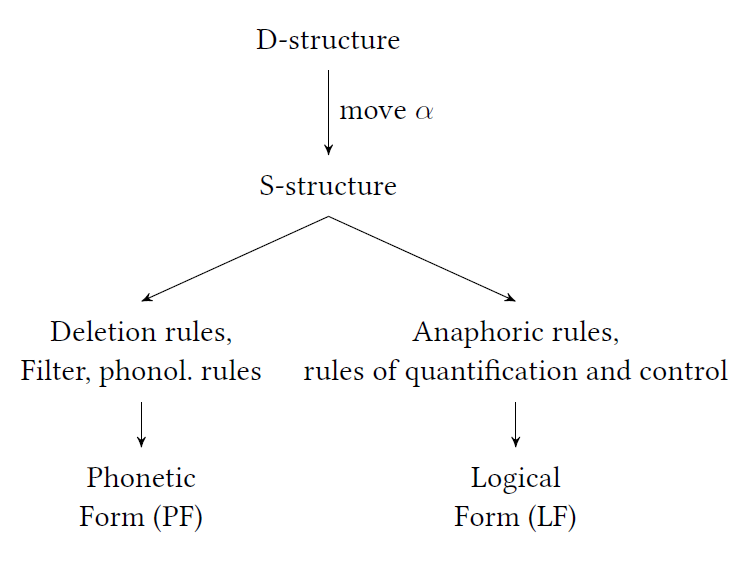
\includegraphics[scale=.43]{material/11tmodell}
%	\caption{T-Modell \citep[vgl.][]{MuellerS15b}}
%\end{figure}
%	
%\end{frame}

\begin{frame}
	%\frametitle{T-Modell}
	
	\begin{figure}
		%\begin{tikzpicture}
		%\node at (0,0) {D-structure};
		%\draw[->] (0,-0.3)--(0,-1.5);
		%\node[right] at (0,-0.9) {move $\alpha$};
		%\node at (0,-1.8) {S-structure};
		%\draw[->] (0,-2.1)--(-1.5-3);
		%\draw[->] (0,-2.1)--(1.5,-3);
		%\end{tikzpicture}
		\begin{forest}
			sm edges,
			[D-structure, [S-structure,edge label={node[midway,right]{move $\alpha$} }
			[{Deletion rules,}\\{Filter, phonol. rules} [Phonetic Form (PF)], align=center]
			[{Anaphoric rules,}\\{rules of quantification and control}, align=center [Logical Form (LF)] ]
			]]
		\end{forest}
		\caption{T-Modell \citep[vgl.][]{MuellerS15b}}
	\end{figure}
	
\end{frame}


%%%%%%%%%%%%%%%%%%%%%%%%%%%%%%%%%%
%%%%%%%%%%%%%%%%%%%%%%%%%%%%%%%%%%
\subsection{Funktionale Phrasen II}

\iftoggle{sectoc}{
	\frame{
		%\begin{multicols}{2}
		\frametitle{~}
		\tableofcontents[currentsubsection,subsubsectionstyle=hide]
		%\end{multicols}
	}
}

%%%%%%%%%%%%%%%%%%%%%%%%%%%%%%%%%%
\begin{frame}
	\frametitle{Funktionale Phrasen II}
	
	\begin{itemize}
		\item Bisher \ras Nebensatzstellung im Deutschen
		\item Wann kommt die NS-Stellung vor? \ras Complementizer!
		
		\eal
		\ex[]{(Ich denke,) \alertred{dass} Syntax Spaß machen sollte.}
		\ex[]{Syntax \alertred{sollte} Spaß machen.}
		\ex[]{(Ich frage mich,) \alertred{ob} der Winter jemals enden wird.}
		\ex[]{Der Winter \alertred{wird} niemals enden.}
		\ex[*]{Der Winter \alertred{ob wird} niemals enden.}
		\zl
		
		\item Complementizer und finite Verben (in V2- und V1-Sätzen) sind \textbf{komplementär}!
		
	\end{itemize}
	
\end{frame}


%%%%%%%%%%%%%%%%%%%%%%%%%%%%%%%%%%
%%%%%%%%%%%%%%%%%%%%%%%%%%%%%%%%%%
\subsubsection{Complementizer Phrase}
%\frame{
%\frametitle{~}
%	\tableofcontents[currentsection]
%}

%%%%%%%%%%%%%%%%%%%%%%%%%%%%%%%%%%
\begin{frame}
	\frametitle{Complementizer Phrase (CP)}
	
	\begin{itemize}
		\item C nimmt eine IP als Komplement
	\end{itemize}
	
	\begin{minipage}[b]{0.45\textwidth}
		\begin{figure}
			\centering
			\scalebox{.6}{
				\begin{forest}
					sm edges,
					[IP [DP [Peter,roof]]
					[\MyPxbar{I} [VP 
					[\MyPxbar{V} [DP [den Wagen,roof]]
					[\zerobar{V} [gekauft]]
					]]
					[I [hat]]
					]
					]
				\end{forest}
			}
			\caption{NS als IP}	
		\end{figure}		
	\end{minipage}  
	%  
	\pause
	%
	\begin{minipage}[b]{0.45\textwidth}
		\begin{figure}
			\centering
			\scalebox{.6}{
				\begin{forest}
					sm edges,
					[CP	[\MyPxbar{C}	[\zerobar{C} [\alertred{dass}\\ \alertred{ob}\\ \alertred{weil}]]	
					[IP [DP [Peter,roof]]
					[\MyPxbar{I} [VP
					[\MyPxbar{V} [DP [den Wagen,roof]]
					[\zerobar{V} [gekauft]]
					]]
					[\zerobar{I} [\alertgreen{hat}]]
					]
					]
					]
					]
				\end{forest}
			}
			\caption{NS als CP}	
		\end{figure}		
	\end{minipage}  
	
	\nocite{Fries&MyP16i}
	
\end{frame}


%%%%%%%%%%%%%%%%%%%%%%%%%%%%%%%%%%
\begin{frame}
	\frametitle{Complementizer Phrase}
	
	\begin{itemize}
		\item Die CP ist für den Satzmodus zuständig.
		\begin{itemize}
			\item Eingebetteter Satz
			\item Eingebetteter Fragesatz
			\item Deklarativsatz
			\item E- oder K-Fragesatz
			\item Imperativsatz
		\end{itemize}
	\end{itemize}
\end{frame}


%%%%%%%%%%%%%%%%%%%%%%%%%%%%%%%%%%
\begin{frame}
	%\frametitle{Complementizer Phrase}
	
	\begin{itemize}
		\item Die CP bestimmt die \textbf{Form} der IP. \ras Finit
	\end{itemize}
	
	\begin{figure}[b]
		
		\begin{minipage}[b]{0.45\textwidth}
			\centering
			\tiny{
				\begin{forest}
					sm edges,
					[*CP	[\MyPxbar{C}	[\zerobar{C} [dass]]
					[IP [DP [Peter,roof]]
					[\MyPxbar{I} [VP 
					[\MyPxbar{V} [DP [den Wagen,roof]]
					[\zerobar{V} [\alertgreen{kaufen}]]{\draw[<-,HUred] (.south east)--++(0em,-1.5ex)--++(+3em,0pt)
						node[anchor=west,align=center]{infinit};}
					]]
					[\zerobar{I} [$\emptyset$]]
					]
					]
					]
					]		
				\end{forest}
			}
			\caption{Ungrammatisch}	
		\end{minipage}  
		%  
		%
		\begin{minipage}[b]{0.45\textwidth}
			\centering
			\tiny{
				\begin{forest}
					sm edges,
					[CP	[\MyPxbar{C}	[\zerobar{C} [dass]]	
					[IP [DP [Peter,roof]]
					[\MyPxbar{I} [VP 
					[\MyPxbar{V} [DP [den Wagen,roof]]
					[\zerobar{V} [t$_{i}$]]
					]]
					[\zerobar{I} [\alertgreen{kauft}$_{i}$]]{\draw[<-,HUred] (.south east)--++(0em,-1.5ex)--++(+2em,0pt)
						node[anchor=west,align=center]{finit};}
					]
					]
					]
					]
				\end{forest}
			}
			\caption{Grammatisch}	
		\end{minipage}  
		
	\end{figure}
	
\end{frame}


%%%%%%%%%%%%%%%%%%%%%%%%%%%%%%%%%%
\begin{frame}
	%\frametitle{Complementizer Phrase}
	
	\begin{itemize}
		\item Korrelation zwischen \textbf{Verbzweit- und Verbletztstruktur}
		\item Kopfbewegung
	\end{itemize}
	
	
	\begin{minipage}[b]{0.49\textwidth}
		\begin{figure}
			\centering
			\tiny{
				\begin{forest}
					sm edges,
					[CP	[\MyPxbar{C}	[\zerobar{C} [\alertgreen{dass}]]{\draw[<-,HUred] (.south west)--++(0em,-2.5ex)--++(-1.5em,0pt)
						node[anchor=east,align=center]{besetzt! \ras \\ keine I-C-Bewegung};}
					[IP [DP [Peter,roof]]
					[\MyPxbar{I} [VP 
					[\MyPxbar{V} [DP [den Wagen,roof]]
					[\zerobar{V} [t$_{i}$]]
					]]
					[\zerobar{I} [\alertgreen{kauft$_{i}$}]]
					]
					]
					]
					]		
				\end{forest}
			}
			\caption{V-I-Bewegung}	
		\end{figure}		
	\end{minipage}  
	%  
	%
	\begin{minipage}[b]{0.49\textwidth}
		\begin{figure}
			\centering
			\tiny{
				\begin{forest}
					sm edges,
					[CP	[\MyPxbar{C}	[\zerobar{C} [\alertgreen{kauft$_{i}$}]]{\draw[<-,HUred] (.south west)--++(0em,-2.5ex)--++(-1.5em,0pt)
						node[anchor=east,align=center]{frei! \ras \\ I-C-Bewegung};}
					[IP [DP [Peter,roof]]
					[\MyPxbar{I} [VP 
					[\MyPxbar{V} [DP [den Wagen,roof]]
					[\zerobar{V} [t$_{i}$]]
					]]
					[\zerobar{I} [\alertgreen{t$_{i}$}]]
					]
					]
					]
					]
				\end{forest}
			}
			\caption{V-I-C-Bewegung}
		\end{figure}			
	\end{minipage}  
	
\end{frame}


%%%%%%%%%%%%%%%%%%%%%%%%%%%%%%%%%%
\begin{frame}
	
	\begin{itemize}
		\item \textbf{Weitere Position} für Verbzweitsätze \ras aber \textbf{nur eine} Phrasenposition
		\ea[*]{[Den Wagen] [Peter] kauft gestern.}
		\z
		
	\end{itemize}
	
	\begin{figure}[b]
		
		\begin{minipage}[b]{0.49\textwidth}
			\centering
			\scalebox{.55}{
				\begin{forest}
					sm edges,
					[CP	[\alertgreen{DP$_{i}$} [Peter,roof]]{\draw[<-,HUred] (.south west)--++(0em,-1.5ex)--++(-2em,0pt)
						node[anchor=east,align=center]{Phrase};}
					[\MyPxbar{C} [\zerobar{C} [kauft$_{ii}$]]
					[IP 
					[,empty nodes [\alertgreen{t$_{i}$}]]
					[\MyPxbar{I} [VP 
					[\MyPxbar{V} [DP [den Wagen,roof]]
					[\zerobar{V} [t$_{ii}$]]
					]]
					[\zerobar{I} [t$_{ii}$]]
					]
					]
					]
					]		
				\end{forest}
			}
			\caption{Subjektbewegung}	
		\end{minipage}  
		%%
		\pause
		%%
		\begin{minipage}[b]{0.49\textwidth}
			\centering
			\scalebox{.55}{
				\begin{forest}
					sm edges,
					[CP	[\alertgreen{DP$_{ii}$} [den Wagen,roof]]{\draw[<-,HUred] (.south west)--++(0em,-1.5ex)--++(-2em,0pt)
						node[anchor=east,align=center]{Phrase};}
					[\MyPxbar{C}	[\zerobar{C} [kauft$_{i}$]]
					[IP [DP [Peter,roof]]
					[\MyPxbar{I} [VP 
					[\MyPxbar{V} 
					[,empty nodes [\alertgreen{t$_{ii}$}]]
					[\zerobar{V} [t$_{i}$]]
					]]
					[\zerobar{I} [t$_{i}$]]
					]
					]
					]
					]
				\end{forest}
			}
			\caption{Objektbewegung}	
		\end{minipage}  
		
	\end{figure}
	
\end{frame}


%%%%%%%%%%%%%%%%%%%%%%%%%%%%%%%%%%
\begin{frame}
	\frametitle{Complementizer Phrase}
	
	\begin{itemize}
		\item Die CP ist für den \textbf{Satzmodus} und die \textbf{illokutionäre Kraft} zuständig.
	\end{itemize}
	
	\begin{figure}[b]
		
		\begin{minipage}[b]{0.45\textwidth}
			\centering
			\scriptsize{
				\begin{forest}
					MyP edges,
					[CP [$\emptyset$]{\draw[<-,HUred] (.south west)--++(0em,-1.5ex)--++(-2em,0pt)
						node[anchor=east,align=center]{leer};}
					[C' [C [dass]]{\draw[<-,HUred] (.south west)--++(0em,-1.5ex)--++(-2em,0pt)
						node[anchor=east,align=center]{Subjunktion};}
					[IP [Peter den Wagen kauft,roof]]]]
				\end{forest}
			}
			\caption{Eingebetteter Satz}	
		\end{minipage}  
		%  
		\pause            
		%         
		\begin{minipage}[b]{0.45\textwidth}
			\centering
			\scriptsize{
				\begin{forest}
					MyP edges,
					[CP [$\emptyset$]{\draw[<-,HUred] (.south west)--++(0em,-1.5ex)--++(-2em,0pt)
						node[anchor=east,align=center]{leer};}
					[C' [C [kauft$_{i}$]]{\draw[<-,HUred] (.south west)--++(0em,-1.5ex)--++(-2em,0pt)
						node[anchor=east,align=center]{Verb};}
					[IP [Peter den Wagen t$_{i}$,roof]]]]
				\end{forest}
			}
			\caption{Entscheidungsfrage}
		\end{minipage}  
		
	\end{figure}
	
\end{frame}


%%%%%%%%%%%%%%%%%%%%%%%%%%%%%%%%%%
\begin{frame}
	\frametitle{Complementizer Phrase}
	
	\begin{itemize}
		\item Die CP ist für den \textbf{Satzmodus} und die \textbf{illokutionäre Kraft} zuständig.
	\end{itemize}
	
	\begin{figure}[b]
		
		\begin{minipage}[b]{0.45\textwidth}
			\centering
			\scriptsize{
				\begin{forest}
					MyP edges,
					[CP [DP$_{ii}$ [was,roof]]{\draw[<-,HUred] (.south west)--++(0em,-1.5ex)--++(-2em,0pt)
						node[anchor=east,align=center]{W-Wort};}
					[C' [C [kauft$_{i}$]]{\draw[<-,HUred] (.south west)--++(0em,-1.5ex)--++(-2em,0pt)
						node[anchor=east,align=center]{Verb};}
					[IP [Peter t$_{ii}$ t$_{i}$,roof]]]]
				\end{forest}
			}
			\caption{Konstituentenfrage}	
		\end{minipage}  
		%  
		\pause            
		%         
		\begin{minipage}[b]{0.49\textwidth}
			\centering
			\scriptsize{
				\begin{forest}
					MyP edges,
					[CP [DP$_{ii}$ [Den Wagen,roof]]{\draw[<-,HUred] (.south west)--++(0em,-1.5ex)--++(-2em,0pt)
						node[anchor=east,align=center]{Konstituente};}
					[C' [C [kauft$_{i}$]]{\draw[<-,HUred] (.south west)--++(0em,-1.5ex)--++(-2em,0pt)
						node[anchor=east,align=center]{Verb};}
					[IP [Peter t$_{ii}$ t$_{i}$,roof]]]]
				\end{forest}
			}
			\caption{Aussagesatz}
		\end{minipage}  
		
	\end{figure}
	
\end{frame}


%%%%%%%%%%%%%%%%%%%%%%%%%%%%%%%%%%
%%%%%%%%%%%%%%%%%%%%%%%%%%%%%%%%%%
\subsection{Erklärungspotential}

\iftoggle{sectoc}{
	\frame{
		%\begin{multicols}{2}
		\frametitle{~}
		\tableofcontents[currentsubsection,subsubsectionstyle=hide]
		%\end{multicols}
	}
}

%%%%%%%%%%%%%%%%%%%%%%%%%%%%%%%%%%%
\begin{frame}
	\frametitle{Erklärungspotential}
	
	\begin{itemize}
		\item Warum ist eine \textbf{VP mit Subjekt} nicht möglich?
		\eal 
		\ex[]{\dots\ (dass) [Peter den Wagen \alertred{kauft}]$_{IP}$.}
		\ex[*]{\dots\ (dass) [Peter den Wagen \alertred{kaufen}]$_{VP}$.}
		\zl
		
		\pause
		\begin{itemize}
			\item \textbf{Kasus} und \textbf{$\theta$-Rolle} werden \textbf{strukturell} vergeben.
			\item[]
			\item Erst durch die \textbf{Subjekt-Verb-Kongruenz} erhält das Subjekt \textsc{nom}-Kasus.
			\item[]
			\item Subjekt-Verb-Kongruenz geschieht durch die \textbf{SpecIP-I$^{0}$-Relation} (strukturelle/lokale Relation).
		\end{itemize}
	\end{itemize}		
	
\end{frame}


%%%%%%%%%%%%%%%%%%%%%%%%%%%%%%%%%%%
\begin{frame}
	
	\begin{itemize}
		\item Warum ist eine \textbf{VP mit Subjekt} nicht möglich?
		\eal 
		\ex[]{\dots\ (dass) [Peter den Wagen \alertred{kauft}]$_{IP}$.}
		\ex[*]{\dots\ (dass) [Peter den Wagen \alertred{kaufen}]$_{VP}$.}
		\zl
		
	\end{itemize}
	
	\begin{figure}[b]
		%	\begin{minipage}[b]{0.80\textwidth}
		\centering
		\scriptsize{
			\begin{forest}
				MyP edges,
				[IP 
				[DP [Peter,roof]]{\draw[<-,HUred] (.north west)--++(0em,+1.5ex)--++(-2em,0pt)
					node[anchor=east,align=center]{\textsc{agens}- \& \\ \textsc{akk}-Vergabe};}
				[\MyPxbar{I} 
				[VP 					
				[\MyPxbar{V} 
				[DP [den Wagen,roof]]{\draw[<-,HUred] (.north west)--++(0em,+1.5ex)--++(-2em,0pt)
					node[anchor=east,align=center]{\textsc{patiens}- \& \\ \textsc{akk}-Vergabe};}
				[\zerobar{V} [gekauft]]
				]
				]
				[\zerobar{I} [hat]]
				]
				]
			\end{forest}
		}
		\caption{Position und Funktion im X-Bar-Schema} 
		%  	\end{minipage}  
		
	\end{figure}
	
\end{frame}


%%%%%%%%%%%%%%%%%%%%%%%%%%%%%%%%%%%
\begin{frame}
	\frametitle{Erklärungspotential}
	
	
	\begin{itemize}
		\item Warum ist die \textbf{Vorfeldbesetzung durch VP mit Subjekt} nicht möglich?
		\eal 
		\ex[]{[Den Wagen \alertred{gekauft}]$_{VP}$ hat Peter gestern.}
		\ex[*]{[Peter den Wagen \alertred{gekauft}]$_{VP}$ hat gestern.}
		\zl
		
		\pause
		\item Damit das Subjekt sichtbar (overt realisiert) wird, muss es \textbf{in SpecIP} \textsc{nom} \textbf{erhalten} \ras Es ist nicht (mehr) in der VP!
		
	\end{itemize}		
	
	\pause
	\begin{itemize}
		\item \textbf{Gewinn} \ras Elegante und restriktive Theorie \nocite{Haspelmath94a}
		
		\begin{itemize}
			\item Keine \textbf{Köpfe} ohne Phrasen
			\item Keine \textbf{Phrasen} ohne Köpfe (exozentrische Phrasen)
			\item Strukturelle \textbf{Position} bestimmt Funktion
			\item \textbf{Einheitlichkeit} der X-Bar-Struktur
		\end{itemize}		
		
	\end{itemize}
	
\end{frame}


%%%%%%%%%%%%%%%%%%%%%%%%%%%%%%%%%%%
\begin{frame}
	
	\begin{itemize}
		\item \textbf{Grammatikalisierung} \ras ein seltenes Argument \citep{Haspelmath94a}
		\item Hilfsverben, Tempus- und Aspektaffixe werden \textbf{aus Vollverben} grammatikalisiert \ras \textbf{Unterschied zwischen Wort oder Affix} ist nicht von Bedeutung.
		\item Die \textbf{Kopf-Dependent-Relation} bleibt bei der Grammatikalisierung immer erhalten \ras Hilfsverben und weitere Affixe sind Köpfe.
	\end{itemize}
	
	
	\begin{figure}[b]
		
		\begin{minipage}[b]{0.40\textwidth}
			\centering
			\scalebox{.8}{
				\begin{forest}
					MyP edges,
					[VP [DP [Julia,roof]]
					[\MyPxbar{V} [VP [cantare,roof]]
					[\zerobar{V} [\alertgreen{habet}]]		{\draw[<-,HUred] (.south east)--++(0em,-1.5ex)--++(+2em,0pt)
						node[anchor=west,align=center]{Kopf};}
					]
					]
				\end{forest}
			}
			\caption{Latein}	
		\end{minipage}  
		%  
		\pause            
		%         
		\begin{minipage}[b]{0.40\textwidth}
			\centering
			\scalebox{.8}{
				\begin{forest}
					MyP edges,
					[IP [DP [Julia,roof]]
					[\MyPxbar{I} [VP [cant-,roof]]
					[\zerobar{I} [\alertgreen{-ará}]]{\draw[<-,HUred] (.south east)--++(0em,-1.5ex)--++(+2em,0pt)
						node[anchor=west,align=center]{Kopf};}
					]
					]
				\end{forest}
			}
			\caption{Spanisch}
		\end{minipage}  
		
	\end{figure}
	
	
\end{frame}


%%%%%%%%%%%%%%%%%%%%%%%%%%%%%%%%%%
%%%%%%%%%%%%%%%%%%%%%%%%%%%%%%%%%%
\subsection{Mehr funktionale Kategorien}

\iftoggle{sectoc}{
	\frame{
		%\begin{multicols}{2}
		\frametitle{~}
		\tableofcontents[currentsubsection,subsubsectionstyle=hide]
		%\end{multicols}
	}
}


%%%%%%%%%%%%%%%%%%%%%%%%%%%%%%%%%%%
%\begin{frame}
%\frametitle{Mehr funktionale Kategorien}
%\nocite{Lenerz93a}
%
%\begin{figure}[b]
%	\begin{minipage}[b]{0.48\textwidth}
%		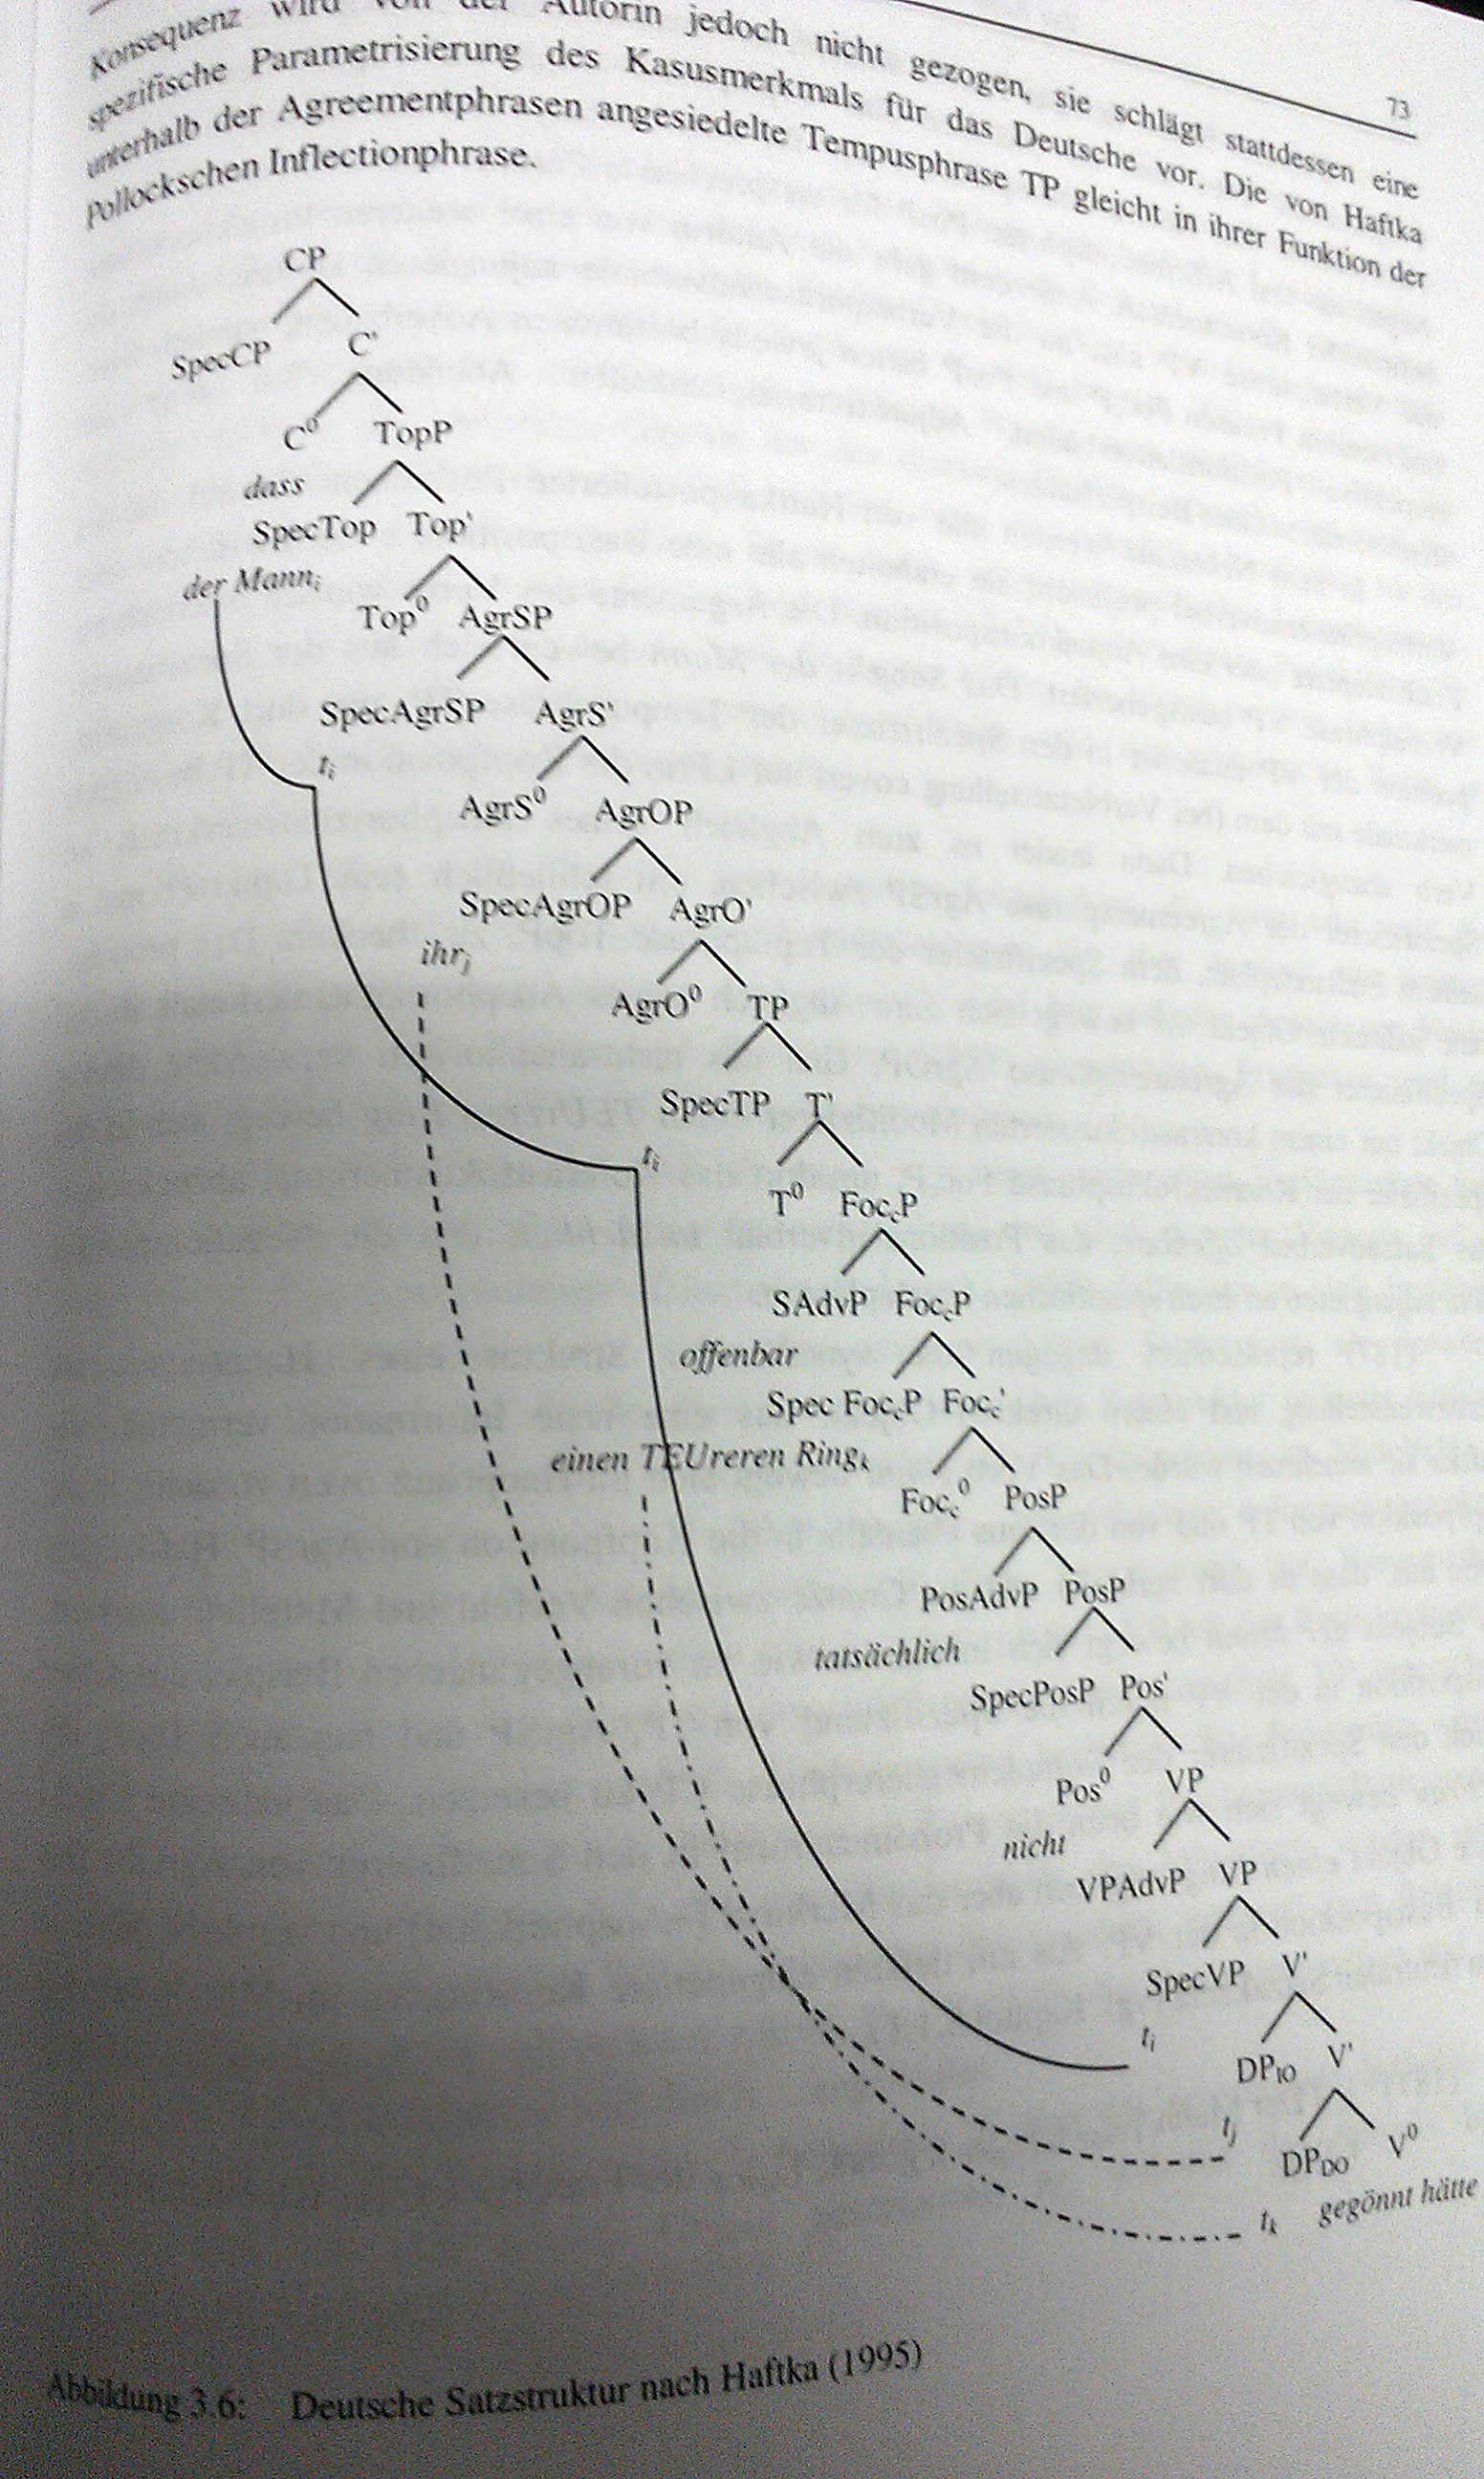
\includegraphics[scale=0.06]{material/Haftka95CP}
%		\caption{CP-Struktur (Haftka 1995)}
%		%\label{Zeichen1}
%	\end{minipage}
%	%
%	%				
%	\begin{minipage}[b]{0.48\textwidth}
%		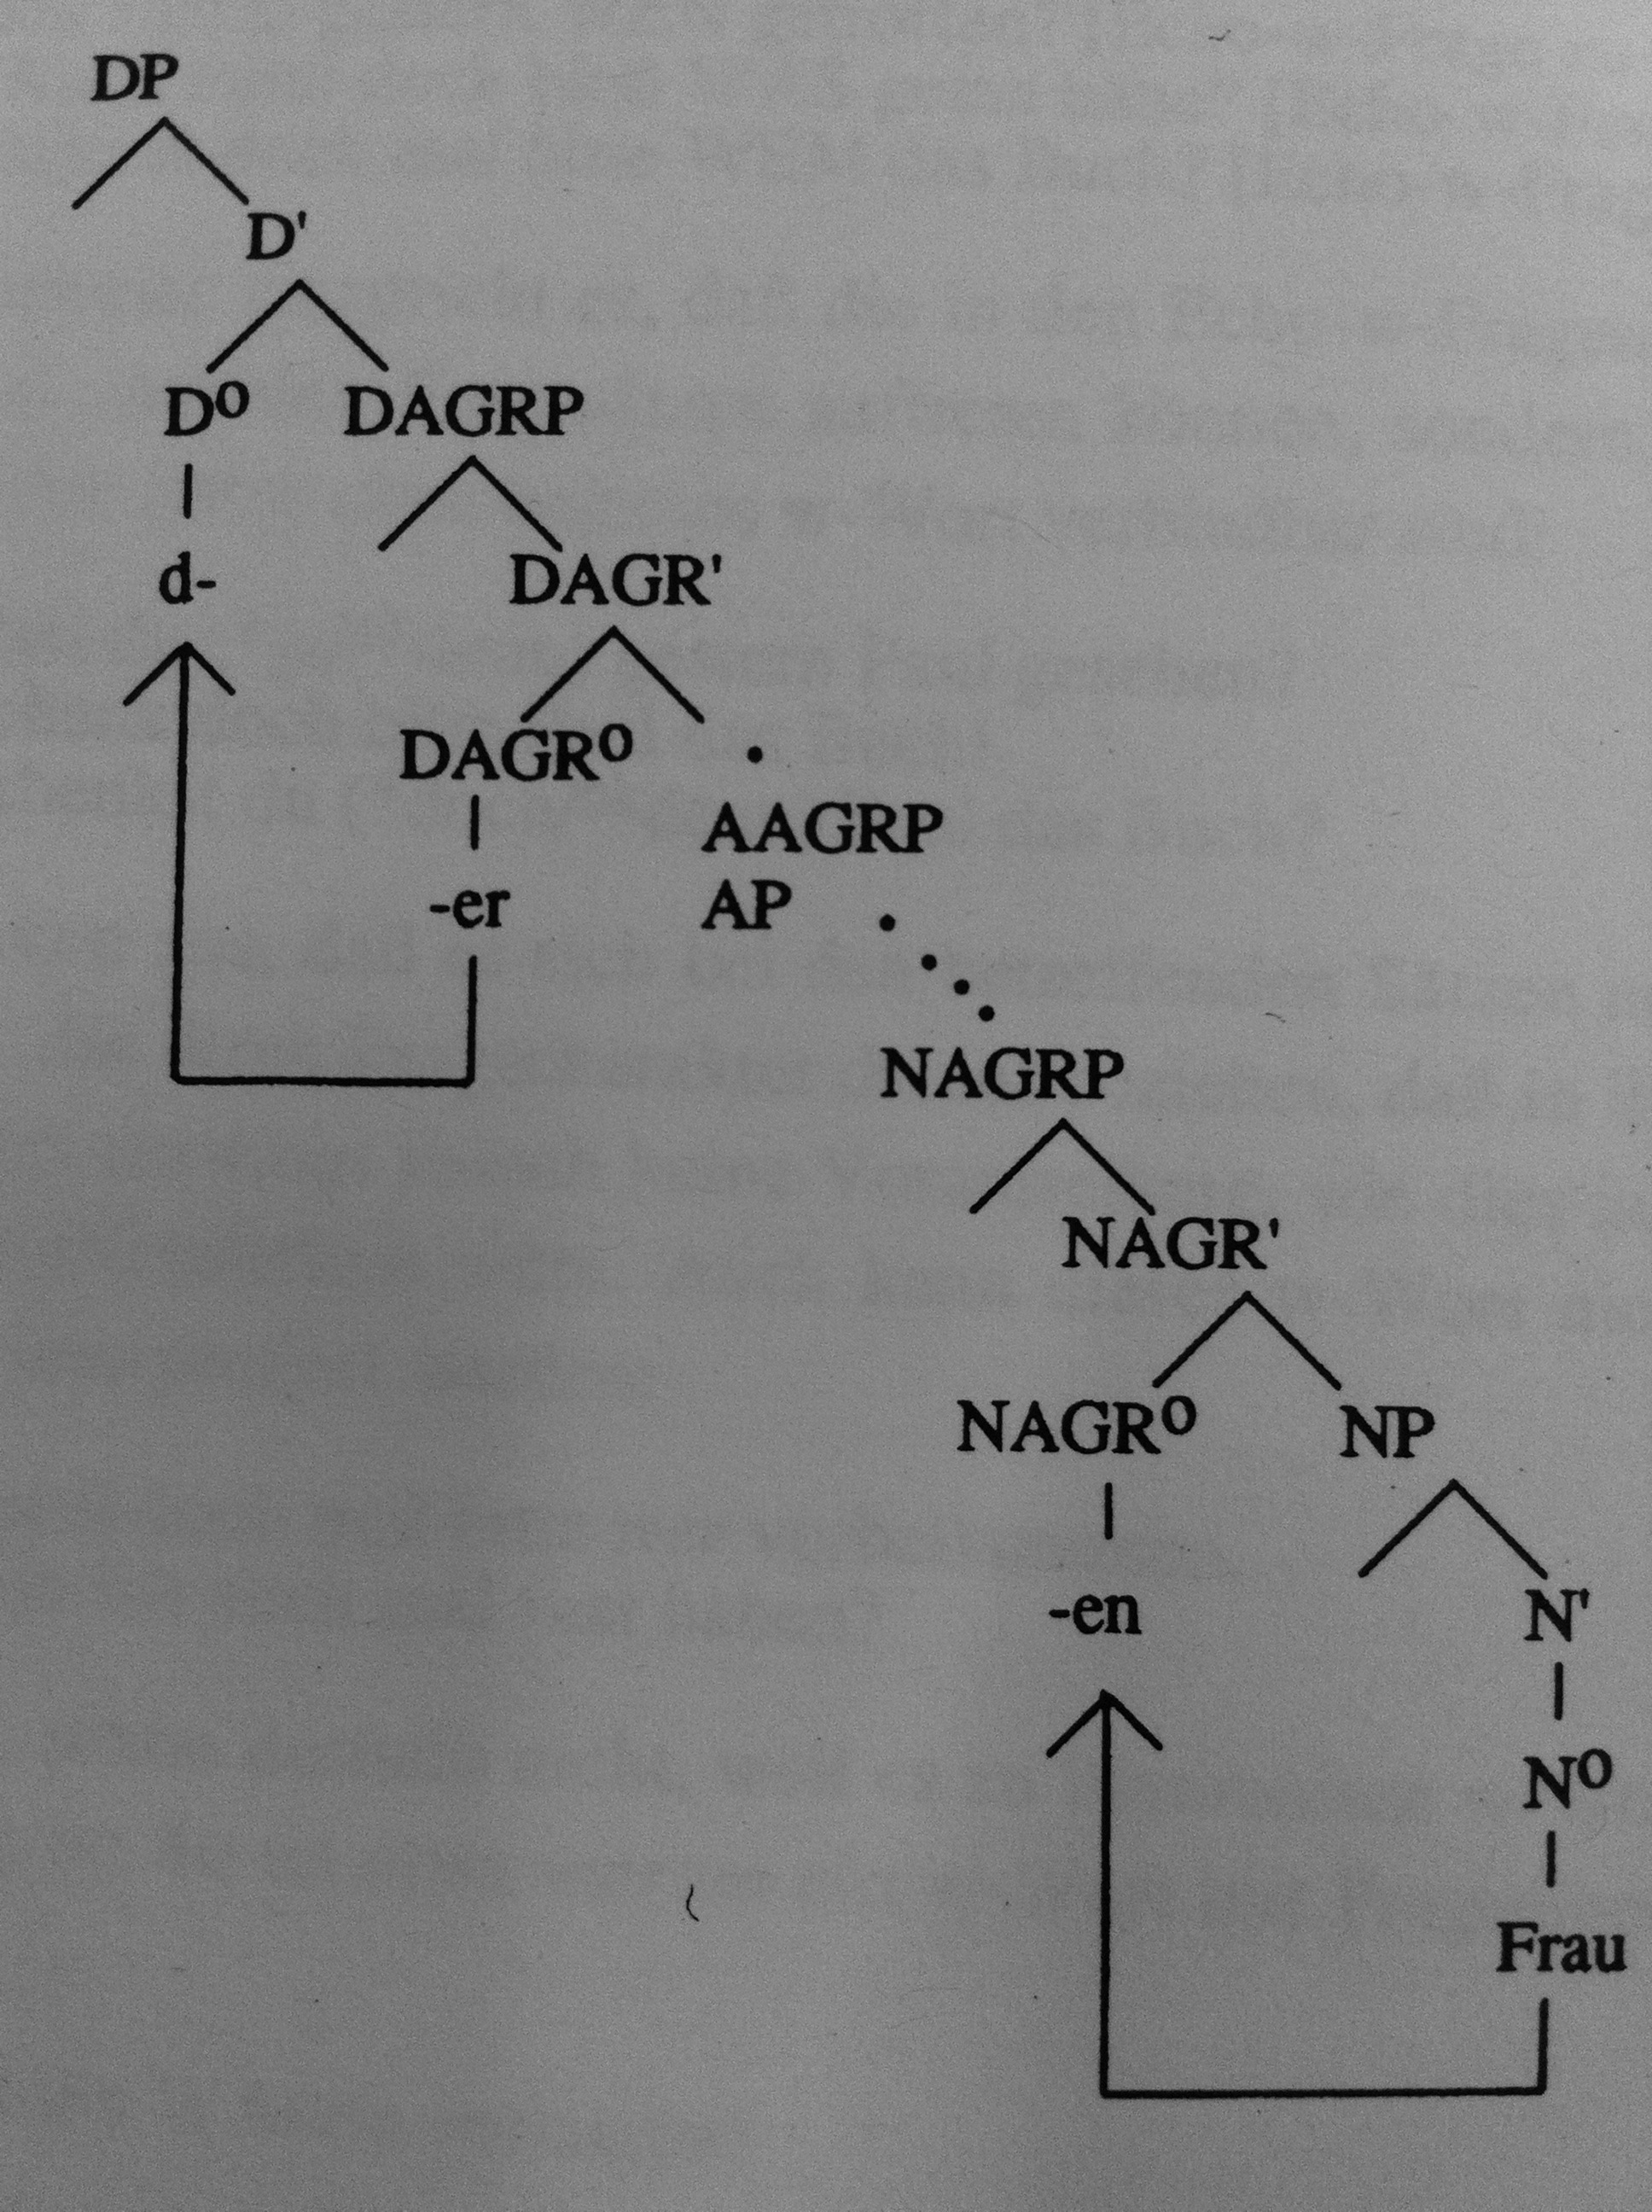
\includegraphics[scale=0.06]{material/Lenerz93DP}
%		\caption{DP-Struktur \citep{Lenerz93a}}
%		%\label{Zeichen2}
%	\end{minipage}                        
%\end{figure}
%
%\end{frame}


\begin{frame}
	\nocite{Lenerz93a}
	
	\begin{minipage}[c]{0.48\textwidth}
		\begin{figure}
			\centering
			\scalebox{.45}{\begin{forest}MyP edges,
					[DP
					[]
					[D'
					[\zerobar{D} [d-, name=d] ]
					[DAGRP
					[]
					[DAGRP'
					[\zerobar{DAGRP} [-er, name=er] ]
					[{AAGRP}\\{AP}, align=center [NAGRP, edge=dotted
					[]
					[NAGR'
					[\zerobar{NAGR} [-en, name=en] ]
					[NP
					[]
					[N' [\zerobar{N} [Frau, name=Frau] ] ]
					]
					]
					] ]
					]
					]
					] ]{
						\draw[->] (Frau) to [out=south west, in=south] (en.south);
						\draw[->] (er) to [out=south west, in=south] (d.south);}
			\end{forest}}
			\caption{DP-Struktur \citep{Lenerz93a}}
		\end{figure}
	\end{minipage}
	%
	%				
	\begin{minipage}[c]{0.48\textwidth}
		\begin{figure}
			\centering 
			\scalebox{.19}{	\begin{forest}
					[CP
					[SpecCP]
					[C'
					[{\zerobar{C}}\\{dass}, align=center]
					[TopP
					[SpecTop \\ \textit{der Mann\textsubscript{i}}, align=center, name=Mann]
					[Top'
					[\zerobar{Top}]
					[AgrSP
					[SpecAgrSP \\ t\textsubscript{i}, align=center, name=Agr]
					[AgrS'
					[\zerobar{AgrS}]
					[AgrOP
					[SpecAgrOP \\ \textit{ihr\textsubscript{j}}, align=center, name=ihr]
					[AgrO'
					[\zerobar{AgrO}]
					[TP
					[SpecTP \\ t\textsubscript{i}, align=center, name=i1]
					[T'
					[\zerobar{T}]
					[Foc\textsubscript{c}P
					[SAdvP\\ \textit{offenbar}, align=center]
					[Foc\textsubscript{c}P
					[SpecFoc\textsubscript{c}P \\ \textit{einen TEUeren Ring\textsubscript{k}}, align=center, name=ring]
					[Foc\textsubscript{c}'
					[\zerobar{Foc\textsubscript{c}}]
					[PosP
					[PosAdvP \\ \textit{tatsächlich}, align=center]
					[PosP
					[SpecPosP]
					[Pos'
					[\zerobar{Pos}\\nicht, align=center]
					[VP	
					[VPAdvP]
					[VP
					[SpecVP\\ t\textsubscript{i}, align=center, name=i2]
					[V'
					[DP\textsubscript{IO} \\ t\textsubscript{j}, align=center, name=j]
					[V'
					[DP\textsubscript{DO} \\ t\textsubscript{k}, align=center, name=k]
					[\zerobar{V}\\\textit{gegönnt hätte}, align=center]
					]
					]
					]
					]
					]
					]
					]
					]
					]	
					]
					]
					]			
					]
					]
					]
					]
					]
					]
					]
					]
					{\draw (i2) to [out=south west, in=south] (i1) to [out=south west, in=south] (Agr) to [out=south west, in=south] (Mann);
						\draw[dashed, thick] (j) to [out=south west, in=south] (ihr);
						\draw[dotted, thick] (k) to [out=south west, in=south] (ring);
					}
			\end{forest}}
			\caption{CP-Struktur (Haftka 1995)}
		\end{figure}
	\end{minipage}                        
	
\end{frame}

%%%%%%%%%%%%%%%%%%%%%%%%%%%%%%%%%%
%%%%%%%%%%%%%%%%%%%%%%%%%%%%%%%%%%
\subsection{Übung}

\iftoggle{sectoc}{
	\frame{
		%\begin{multicols}{2}
		\frametitle{~}
		\tableofcontents[currentsubsection,subsubsectionstyle=hide]
		%\end{multicols}
	}
}


%%%%%%%%%%%%%%%%%%%%%%%%%%%%%%%%%%%
%%%%%%%%%%%%%%%%%%%%%%%%%%%%%%%%%%%

%%%%%%%%%%%%%%%%%%%%%%%%%%%%%%%%%%%
\begin{frame}
	\frametitle{Übung}
	
	\begin{itemize}
		\item Erklären Sie mithilfe des X-Bar-Schemas die \textbf{Ambiguität} im folgenden Satz:
		
		\ea Das Kind küsst die Mama.
		\z
		
	\end{itemize}
\end{frame}


%%%%%%%%%%%%%%%%%%%%%%%%%%%%%%%%%%%

\iftoggle{ue-loesung}{
	
	%%%%%%%%%%%%%%%%%%%%%%%%%%%%%%%%%%%
%06g Syntax ue-loesung01
%%%%%%%%%%%%%%%%%%%%%%%%%%%%%%%%%

\begin{frame}
\frametitle{Übung -- Lösung}


\begin{minipage}[b]{0.29\textwidth}
	\centering
	\scalebox{0.55}{
		\begin{forest}
			MyP edges,
			[CP
			[DP$ _{k} $[Das Kind, roof]]
			[\MyPxbar{C} 
			[\zerobar{C}[küsst$ _{i} $]]
			[IP
			[\alertgreen{t$_{k}$}]
			[\MyPxbar{I}
			[VP [\MyPxbar{V}
			[DP[die Mama, roof]]
			[\zerobar{V}[t$ _{i} $]]
			]
			]
			[\zerobar{I}[t$ _{i} $]]
			]
			]
			]
			]
		\end{forest}
		}
\end{minipage}
%
%
\begin{minipage}[b]{0.31\textwidth}
	\centering
	\scalebox{0.55}{
		\begin{forest}
			MyP edges,
			[CP
			[DP$ _{k} $[Das Kind, roof]]
			[\MyPxbar{C} 
			[\zerobar{C}[küsst$ _{i} $]]
			[IP
			[DP[die Mama, roof]]
			[\MyPxbar{I}
			[VP [\MyPxbar{V}
			[\alertgreen{t$_{k}$}]
			[\zerobar{V}[t$ _{i} $]]
			]
			]
			[\zerobar{I}[t$ _{i} $]]
			]
			]
			]
			]
		\end{forest}
		}
\end{minipage}
%%
%%
\begin{minipage}[b]{.38\textwidth}


\begin{itemize*}
	\alertgreen{\item {\small \MyPobj{das Kind} und \MyPobj{die Mama} sind im Akkusativ und im Nominativ formgleich (Synkretismus).}}
	\alertgreen{\item {\small Im Dt. kann eine Phrase in die SpecCP-Position bewegt werden.}}
	\alertgreen{\item {\small Wegen des Synkretismus' ist nicht ersichtlich, ob \MyPobj{das Kind} sich aus der SpecIP- oder aus der Schwesterposition von V\MyPup{0} bewegt hat. }}
\end{itemize*}

\end{minipage}
\end{frame}

	
}

%%%%%%%%%%%%%%%%%%%%%%%%%%%%%%%%%%%

\begin{frame}
	\frametitle{Übung}
	
	\begin{itemize}
		
		\item Erklären Sie mithilfe des X-Bar-Schemas, warum der folgende Satz \textbf{ungrammatisch} ist:
		
		\ea Im Auto ich habe heute geschlafen.
		\z
		
	\end{itemize}
\end{frame}



%%%%%%%%%%%%%%%%%%%%%%%%%%%%%%%%%%%

\iftoggle{ue-loesung}{
	
	%%%%%%%%%%%%%%%%%%%%%%%%%%%%%%%%%%%
%06g Syntax ue-loesung02
%%%%%%%%%%%%%%%%%%%%%%%%%%%%%%%%%

\begin{frame}
\frametitle{Übung -- Lösung}

\begin{minipage}[b]{0.45\textwidth}
	\centering
	\scalebox{0.6}{
		\begin{forest}
			MyP edges,
			[CP
			[DP$_{k}$ [Ich,roof]]
			[\MyPxbar{C} [\zerobar{C} [habe$_{i}$]]
			[IP [t$_{k}$]
			[\MyPxbar{I}
			[VP	[AdVP [heute,roof]]
			[VP [PP	[im Auto,roof]]{\draw[->,HUgreen] (.south west)--++(-7em,0em)--++(0em,14em)
				node[anchor=east,align=center]{PP kann nicht \\ bewegt werden};}
			[\MyPxbar{V} [\zerobar{V} [geschlafen t$_{i}$]]]
			]
			]
			[\zerobar{I} [t$_{i}$]]
			]
			]
			]	
			]
		\end{forest}
	}
\end{minipage}  
%            
%         
\begin{minipage}[b]{0.45\textwidth}
\alertgreen{{\small 
	Nur eine Phrase, d.\,h.\ entweder die DP \MyPobj{ich} oder die PP \MyPobj{im Auto}, kann die SpecCP-Position belegen. Da die DP und die PP zusammen nicht eine Phrase bilden, können nicht \textbf{beide} Phrasen in diese Position bewegt werden.
}}
\end{minipage}  

\end{frame}
}

%%%%%%%%%%%%%%%%%%%%%%%%%%%%%%%%%%%

%%%%%%%%%%%%%%%%%%%%%%%%%%%%%%%%%%%
\begin{frame}
	\frametitle{Übung}
	
	\begin{itemize}
		\item Was ist an dieser Struktur misslungen? Beziehen Sie sich in Ihrer Antwort \ua auf die in der Sitzung behandelten Köpfigkeitsmerkmale und Strukturaufbaugesetzmäßigkeiten.
	\end{itemize}
	
	\begin{figure}
		\scalebox{.75}{\begin{forest} sm edges,
				[S
				[VP [V [Tea] ] ]
				[NP
				[P [with]]
				[Det [some]]
				[N [lemon]]
				]
				[PP
				[P [tastes]]
				[NP [Adj [really] ] [N [nice]] ]
				]
				]
		\end{forest}}
		%	\includegraphics[scale=.45]{material/wrongtree}
		\caption{vgl.\ \url{http://specgram.com/CLXV.1/05.cruz-ferreira.know22.html}}
	\end{figure}
	
\end{frame}



%%%%%%%%%%%%%%%%%%%%%%%%%%%%%%%%%%%

\iftoggle{ue-loesung}{
	
	%%%%%%%%%%%%%%%%%%%%%%%%%%%%%%%%%%%
%06g Syntax ue-loesung03
%%%%%%%%%%%%%%%%%%%%%%%%%%%%%%%%%%%
	
\begin{frame}
\frametitle{Übung -- Lösung}


\begin{columns}

\begin{column}{.45\textwidth}
\begin{figure}
	\scalebox{.6}{\begin{forest} sm edges,
			[S
			[VP [V [Tea] ] ]
			[NP
			[P [with]]
			[Det [some]]
			[N [lemon]]
			]
			[PP
			[P [tastes]]
			[NP [Adj [really] ] [N [nice]] ]
			]
			]
	\end{forest}}
	%	\includegraphics[scale=.45]{material/wrongtree}
	\caption{vgl.\ \url{http://specgram.com/CLXV.1/05.cruz-ferreira.know22.html}}
\end{figure}
\end{column}
%%
%%
\begin{column}{.55\textwidth}

\begin{itemize}
	\alertgreen{\item keine binäre Struktur (mehr als zwei Töchter)}
	\alertgreen{\item falsche Kategorien bestimmt (\zB \MyPobj{Tea}: V?)}
	\alertgreen{\item Es gibt Köpfe ohne Phrasen}
	\alertgreen{\item keine Zwischen Projektionen}
	\alertgreen{\item Satz ist exozentrisch}
	\alertgreen{\item \dots}
\end{itemize}

\end{column}
\end{columns}

\end{frame}

	
}


%%%%%%%%%%%%%%%%%%%%%%%%%%%%%%%%%%
%%%%%%%%%%%%%%%%%%%%%%%%%%%%%%%%%%

\subsection{Hausaufgabe}

%%%%%%%%%%%%%%%%%%%%%%%%%%%%%%%%%%%
%%%%%%%%%%%%%%%%%%%%%%%%%%%%%%%%%%%

%%%%%%%%%%%%%%%%%%%%%%%%%%%%%%%%%%
\begin{frame}
	\frametitle{Hausaufgabe}
	
	\begin{itemize}
		\item Geben Sie an, um welchen \textbf{Phrasentyp} es sich bei den folgenden Phrasen handelt, und \textbf{welches Wort} sich in der \textbf{Kopfposition} der Phrasen befindet.
		
		\eal
		\ex viele besorgte Mütter
		\ex den Menschen in Not helfen
		\ex Wasser ohne Kohlensäure
		\ex auf Maria warten
		\ex ob sie heute kommen werden
		\ex Peter seine Traumfrau gefunden hat
		\zl
		
	\end{itemize}
	
\end{frame}

%%%%%%%%%%%%%%%%%%%%%%%%%%%%%%%%%%%

%%%%%%%%%%%%%%%%%%%%%%%%%%%%%%%%%%
\begin{frame}
	\frametitle{Hausaufgabe}
	
	\begin{itemize}
		\item Analysieren Sie die folgenden Phrasen nach dem X-Bar-Schema (ohne Abkürzungen).
		
		\ea Peter schläft.
		\ex Wer schläft?
		\ex Hat sie dir die schwierige Frage nach den Spuren gestellt?
		\ex die fast vor dem Mittagessen erstellte Speisekarte
		\ex weil der Präsident kommt, hat die Polizei die Sicherung des Geländes übernommen
		\z
		
	\end{itemize}
\end{frame}


%%%%%%%%%%%%%%%%%%%%%%%%%%%%%%%%%%%%%%%%%%%%

\iftoggle{ha-loesung}{
	
	%%%%%%%%%%%%%%%
%06g Syntax ha-loesung
%%%%%%%%%%%%%%%%


\begin{frame}
\frametitle{Hausaufgabe -- Lösung}

\begin{itemize}
	\item Geben Sie an, um welchen \textbf{Phrasentyp} es sich bei den folgenden Phrasen handelt, und \textbf{welches Wort} sich in der \textbf{Kopfposition} der Phrasen befindet:
\end{itemize}	

\eal
	\ex viele besorgte Mütter  \pause \hfill \alertgreen{Mütter} \& \alertgreen{NP} oder \alertgreen{viele} \& \alertgreen{DP} \pause 

	\ex den Menschen in Not helfen \pause \hfill \alertgreen{helfen} \& \alertgreen{VP} \pause 
	
	\ex Wasser ohne Kohlensäure \pause \hfill \alertgreen{Wasser} \& \alertgreen{NP} oder \alertgreen{$\emptyset$} \& \alertgreen{DP} \pause 
	
	\ex auf Maria warten \pause \hfill \alertgreen{warten} \& \alertgreen{VP} \pause 
	
	\ex ob sie heute kommen werden \pause \hfill \alertgreen{ob} \& \alertgreen{CP} \pause 
	
	\ex Peter seine Traumfrau gefunden hat \pause \hfill \alertgreen{hat} \& \alertgreen{IP}
\zl

\end{frame}

%%%%%%%%%%%%%%%%%%%%%%%%%%%%%%%%%%%%%%

\begin{frame}
\frametitle{Hausaufgabe -- Lösung}

\begin{minipage}[b]{0.45\textwidth}
	
	{\small Peter schläft.}
	
	\pause
	
	\centering
	\scalebox{0.6}{
		\begin{forest}
		MyP edges,
		[\alertgreen{CP} 
			[\alertgreen{DP$_{k}$} 
				[\alertgreen{Peter},roof]
			]
			[\alertgreen{\MyPxbar{C}}
				[\alertgreen{\zerobar{C}} 
					[\alertgreen{schläft$_{i}$}]
				]
				[\alertgreen{IP} 
					[\alertgreen{t$_{k}$}]
					[\alertgreen{\MyPxbar{I}}
						[\alertgreen{VP} 
							[\alertgreen{\MyPxbar{V}} 
								[\alertgreen{\zerobar{V}} 
									[\alertgreen{t$_{i}$}]
								]
							]
						]
						[\alertgreen{\zerobar{I}} 
							[\alertgreen{t$_{i}$}]
						]
					]
				]
			]
		]
		\end{forest}
	}
\end{minipage}  
%            
%         
\begin{minipage}[b]{0.45\textwidth}
	
	\pause 
	
	{\small Wer schläft?}	
	
	\pause 
	
	\centering
	\scalebox{0.6}{
		\begin{forest}
			MyP edges,
			[\alertgreen{CP} 
			[\alertgreen{DP$_{k}$} [\alertgreen{Wer},roof]
			]
			[\alertgreen{\MyPxbar{C}}
			[\alertgreen{\zerobar{C}} [\alertgreen{schläft$_{i}$}]
			]
			[\alertgreen{IP} [\alertgreen{t$_{k}$}]
			[\alertgreen{\MyPxbar{I}}
			[\alertgreen{VP} [\alertgreen{\MyPxbar{V}} [\alertgreen{\zerobar{V}} [\alertgreen{t$_{i}$}	]]]]
			[\alertgreen{\zerobar{I}} [\alertgreen{t$_{i}$}]]
			]
			]
			]
			]
		\end{forest}
	}
\end{minipage}  

\end{frame}


%%%%%%%%%%%%%%%%%%%%%%%%%%%%%%%%%%
\begin{frame}
\frametitle{Hausaufgabe -- Lösung}

{\small Hat sie dir die schwierige Frage nach den Spuren gestellt?}

\pause

\begin{minipage}[b]{0.45\textwidth}

\centering
\scalebox{0.6}{
	\begin{forest}
		MyP edges,
		[\alertgreen{CP} 
		[\alertgreen{\MyPxbar{C}}
		[\alertgreen{\zerobar{C}} [\alertgreen{Hat$_{i}$}]
		]
		[\alertgreen{IP} [\alertgreen{DP} [\alertgreen{\MyPxbar{D}} [\alertgreen{\zerobar{D}} [\alertgreen{sie}]]]
		]
		[\alertgreen{\MyPxbar{I}}
		[\alertgreen{VP} 
		[\alertgreen{DP} [\alertgreen{\MyPxbar{D}} [\alertgreen{\zerobar{D}} [\alertgreen{dir}]]]]
		[\alertgreen{\MyPxbar{V}} 								
		[\alertgreen{DP}, draw, HUgreen 
		[\alertgreen{die} \dots\ \alertgreen{Spuren},roof]
		]		
		[\alertgreen{\zerobar{V}} [\alertgreen{gestellt}]]
		]
		]
		[\alertgreen{\zerobar{I}} [\alertgreen{t$_{i}$}]]
		]
		]
		]
		]
	\end{forest}
}
\end{minipage}  
%      
\pause  	      
%         
\begin{minipage}[b]{0.45\textwidth}

\centering
\scalebox{0.4}{
	\begin{forest}
		MyP edges,
		[\alertgreen{DP}
		[\alertgreen{\MyPxbar{D}}
		[\alertgreen{\zerobar{D}}[\alertgreen{die}]]
		[\alertgreen{NP}
		[\alertgreen{AP} [\alertgreen{\MyPxbar{A}} [\alertgreen{\zerobar{A}} [\alertgreen{schwierige}]]]]
		[\alertgreen{NP} 
		[\alertgreen{\MyPxbar{N}} 
		[\alertgreen{\zerobar{N}} [\alertgreen{Frage}]]
		[\alertgreen{PP}
		[\alertgreen{\MyPxbar{P}} 
		[\alertgreen{\zerobar{P}} [\alertgreen{nach}]]
		[\alertgreen{DP}
		[\alertgreen{\MyPxbar{D}}
		[\alertgreen{\zerobar{D}} [\alertgreen{den}]]
		[\alertgreen{NP} [\alertgreen{\MyPxbar{N}} [\alertgreen{\zerobar{N}} [\alertgreen{Spuren}]]]]
		]
		]
		]
		]
		]
		]
		]
		]
		]
	\end{forest}
}
\end{minipage}  

\end{frame}


%%%%%%%%%%%%%%%%%%%%%%%%%%%%%%%%%%
\begin{frame}
\frametitle{Hausaufgabe -- Lösung}

{\small die fast vor dem Mittagessen erstellte Speisekarte}

\pause 

\begin{minipage}[b]{0.45\textwidth}

\centering
\scalebox{0.6}{
\begin{forest}
	MyP edges,
	[\alertgreen{DP}
	[\alertgreen{\MyPxbar{D}}
	[\alertgreen{\zerobar{D}}[\alertgreen{die}]]
	[\alertgreen{NP}
	[\alertgreen{AP}
	[\alertgreen{PP}, draw, HUgreen 
	[\alertgreen{fast vor dem Mittagessen},roof]
	%							[AdvP [\MyPxbar{Adv} [\zerobar{Adv} [kurz]]]]
	%							[PP [\MyPxbar{P}
	%									[\zerobar{Adv} [vor]]
	%									[DP [\MyPxbar{D} [\zerobar{D} [dem]]
	%										[NP [\MyPxbar{N} [\zerobar{N} [Mittagessen]]]]
	%										]
	%									]				
	%								]							
	%							]
	]	
	[\alertgreen{AP} [\alertgreen{\MyPxbar{A}} [\alertgreen{\zerobar{A}} [\alertgreen{erstellte}]]]]
	]
	[\alertgreen{NP} [\alertgreen{\MyPxbar{N}} [\alertgreen{\zerobar{N}} [\alertgreen{Speisekarte}]]]
	]
	]
	]
	]
\end{forest}
}
\end{minipage}  
%  
\pause          
%         
\begin{minipage}[b]{0.45\textwidth}

\centering
\scalebox{0.6}{
\begin{forest}
	MyP edges,
	[\alertgreen{PP}
	[\alertgreen{AdvP} [\alertgreen{\MyPxbar{Adv}} [\alertgreen{\zerobar{Adv}} [\alertgreen{fast}]]]]
	[\alertgreen{PP} 
	[\alertgreen{\MyPxbar{P}}
	[\alertgreen{\zerobar{P}} [\alertgreen{vor}]]
	[\alertgreen{DP} [\alertgreen{\MyPxbar{D}} [\alertgreen{\zerobar{D}} [\alertgreen{dem}]]
	[\alertgreen{NP} [\alertgreen{\MyPxbar{N}} [\alertgreen{\zerobar{N}} [\alertgreen{Mittagessen}]]]]
	]
	]				
	]							
	]
	]	
\end{forest}
}
\end{minipage}  

\end{frame}

%%%%%%%%%%%%%%%%%%%%%%%%%%%%%%%%%%
\begin{frame}
	\frametitle{Hausaufgabe -- Lösung}
	
	{\small weil der Präsident kommt, hat die Polizei die Sicherung des Geländes übernommen}

\pause
	
	\centering
	\scalebox{0.35}{
	\begin{forest}
%			sm edges
			[\alertgreen{CP}
			  [\alertgreen{CP$_i$}
			    [\alertgreen{C$'$}
				  [\alertgreen{C} [\alertgreen{weil}]]
				  [\alertgreen{IP}
					[\alertgreen{DP}
					  [\alertgreen{D$'$} 
						[\alertgreen{D} [\alertgreen{der}]]
						[\alertgreen{NP} 
						[\alertgreen{N$'$}
						  [\alertgreen{N} [\alertgreen{Präsident}]]]]]]
					[\alertgreen{I$'$}
					  [\alertgreen{VP} [\alertgreen{V$'$} [\alertgreen{V} [\alertgreen{$t_j$}]]]]
					  [\alertgreen{I} [\alertgreen{kommt$_j$}]]]]]]
			  [\alertgreen{C$'$}
			    [\alertgreen{C} [\alertgreen{hat$_k$}]]
				  [\alertgreen{IP}
					[\alertgreen{DP}
					  [\alertgreen{D$'$} 
						[\alertgreen{D} [\alertgreen{die}]]
						[\alertgreen{NP} 
						[\alertgreen{N$'$}
						  [\alertgreen{N} [\alertgreen{Polizei}]]]]]]
					[\alertgreen{I$'$}
					  [\alertgreen{VP}
%						[\alertgreen{CP} 
						[\alertgreen{$t_i$}]
%						]
%						[\alertgreen{VP}
%						  [\alertgreen{V$'$}
						    [\alertgreen{VP} 
							  [\alertgreen{V$'$} 
								[\alertgreen{DP}
								  [\alertgreen{D$'$} 
									[\alertgreen{D} [\alertgreen{die}]]
									[\alertgreen{NP} 
									  [\alertgreen{N$'$}
										[\alertgreen{N} [\alertgreen{Sicherung}]]
										[\alertgreen{DP}
										  [\alertgreen{D$'$} 
											[\alertgreen{D} [\alertgreen{des}]]
											[\alertgreen{NP} 
											  [\alertgreen{N$'$}
												[\alertgreen{N} [\alertgreen{Geländes}]]]]]]
								]]]]
								[\alertgreen{V} [\alertgreen{übernommen}]]]]
%							[\alertgreen{V} [\alertgreen{$t_k$}]]
%							]
%						]
					]
					  [\alertgreen{I} [\alertgreen{$t_k$}]]]]]]
	\end{forest}}

\end{frame}

	
}



%%%%%%%%%%%%%%%%%%%%%%%%%%%%%%%%%%%
%%%%%%%%%%%%%%%%%%%%%%%%%%%%%%%%%%%
\begin{frame}
	\frametitle{Schluss!}
	
	\begin{figure}
		\includegraphics[scale=.5]{material/11chomksy}
		\caption{Geschafft!}
	\end{figure}
	
\end{frame}

%%%%%%%%%%%%%%%%%%%%%%%%%%%%%%%%%%%%%%%%%%%%%%%%
%% Compile the master file!
%% 		Slides: Antonio Machicao y Priemer
%% 		Course: GK Linguistik
%%%%%%%%%%%%%%%%%%%%%%%%%%%%%%%%%%%%%%%%%%%%%%%%


%%%%%%%%%%%%%%%%%%%%%%%%%%%%%%%%%%%%%%%%%%%%%%%%%%%%
%%%             Metadata                         
%%%%%%%%%%%%%%%%%%%%%%%%%%%%%%%%%%%%%%%%%%%%%%%%%%%%      

\title{Grundkurs Linguistik}

\subtitle{Semantik I}

\author[A. Machicao y Priemer]{
	{\small Antonio Machicao y Priemer}
	\\
	{\footnotesize \url{http://www.linguistik.hu-berlin.de/staff/amyp}}
%	\\
%	\href{mailto:mapriema@hu-berlin.de}{mapriema@hu-berlin.de}}
}

\institute{Institut für deutsche Sprache und Linguistik}

\date{ }

%\publishers{\textbf{6. linguistischer Methodenworkshop \\ Humboldt-Universität zu Berlin}}

%\hyphenation{nobreak}


%%%%%%%%%%%%%%%%%%%%%%%%%%%%%%%%%%%%%%%%%%%%%%%%%%%%
%%%             Preamble's End                   
%%%%%%%%%%%%%%%%%%%%%%%%%%%%%%%%%%%%%%%%%%%%%%%%%%%%      


%%%%%%%%%%%%%%%%%%%%%%%%%      
\huberlintitlepage[22pt]

\iftoggle{toc}{
\frame{
\begin{multicols}{2}
	\frametitle{Inhaltsverzeichnis}\tableofcontents
	%[pausesections]
\end{multicols}
}
}


%%%%%%%%%%%%%%%%%%%%%%%%%%%%%%%%%%
%%%%%%%%%%%%%%%%%%%%%%%%%%%%%%%%%%
%%%%%LITERATURE:

%% Allgemein
\nocite{Glueck&Roedel16a}
\nocite{Luedeling2009a}
\nocite{Meibauer&Co07a} 
\nocite{Repp&Co15a} 

%% Morphologie
%\nocite{Eisenberg04}

%% Syntax
%\nocite{Adger04a}
%\nocite{Altmann&Hofmann08a} % Satztypen & Satzmodi
%\nocite{Altmann93a} % Satztypen & Satzmodi
%\nocite{Brandt&Co06a} 
%\nocite{Fanselow&Sascha87a}
%\nocite{Fanselow&Sascha93a}
%\nocite{Fries&MyP16b} % Akzeptabilität
%\nocite{Fries16a} % Grammatikalität
%\nocite{Fries&MyP16d} % Kompetenz vs Performanz
%\nocite{Fries&MyP16c} % GG
%\nocite{Fries&MyP16a} % X-Bar-Theorie
%\nocite{Fries16e} % Satztyp
%\nocite{Fries16d} % Satzmodus 
\nocite{Grewendorf&Co91a} 
%\nocite{MyP17b} % Kerngrammatik
%\nocite{MyP18a} % Konstituententest
\nocite{MyP18b} % Kopf
%\nocite{MyP18c} % Phrase
%\nocite{MyP18s} % Funktionale Kategorie
\nocite{MyP18t} % Argumentstruktur
%\nocite{MuellerS13f} 
%\nocite{MuellerS15b}
%\nocite{Stechow&Sternefeld88a}
%\nocite{Sternefeld06a}
%\nocite{Sternefeld06b}
%\nocite{Woellstein10a} % Topologisches Feldermodell

%% Semantik & Pragmatik
\nocite{Cresswell91a} %% Basic concepts of semantics
\nocite{Loebner15a} %% Semantics
\nocite{Loebner15b} %% Semantics
\nocite{Lohnstein11} %% Semantics
\nocite{MyP16a} %% Bikonditional
\nocite{MyP16h} %% Merkmalsemantik
\nocite{Fries&MyP16k} %Ambiguität
\nocite{Partee19a} %% History Semantics
\nocite{Partee&Co93a} %% Semantics
\nocite{Schwarz&Chur93} %% Wortrelationen
\nocite{ZimmermannT&Sternefeld13a} %% Semantics


%%%%%%%%%%%%%%%%%%%%%%%%%%%%%%%%%%
%%%%%%%%%%%%%%%%%%%%%%%%%%%%%%%%%%
\begin{frame}
\frametitle{Begleitlektüre}

\begin{itemize}
\item \textbf{obligatorisch:}
	\begin{itemize}
	\item[] AM S.~95--106
	\item[] \citet{Lohnstein11}: Kapitel 4 (S.~34--49)
	\end{itemize}
\end{itemize}
\end{frame}


%%%%%%%%%%%%%%%%%%%%%%%%%%%%%%%%%%%
\section{Semantik I}
%%%%%%%%%%%%%%%%%%%%%%%%%%%%%%%%%%%
%
\subsection{Einführung}

\iftoggle{sectoc}{
	\frame{
		%\begin{multicols}{2}
		\frametitle{~}
		\tableofcontents[currentsubsection,subsubsectionstyle=hide]
		%\end{multicols}
	}
}
%%%%%%%%%%%%%%%%%%%%%%%%%%%%%%%%%%%

\begin{frame}
\frametitle{Einführung}

\begin{itemize}
	\item Semantik: Bedeutungslehre
	\medskip
	\item Teildisziplin der \textbf{Linguistik} 
	\medskip
	\item Aufgabe: \\ Erfassen der \textbf{Bedeutung} von einfachen und zusammengesetzten \textbf{natürlichsprachlichen Ausdrücken} 

\end{itemize}

\end{frame}


%%%%%%%%%%%%%%%%%%%%%%%%%%%%%%%%%%%%%%%%
\begin{frame}
	\frametitle{Einführung}

\begin{itemize}
	\item Durch morphologische und syntaktische Kompetenz \ras System, das eine unendliche Menge von Wörtern und Sätzen repräsentiert
	\medskip
	\item Aufgabe der Semantik: 
	
	\begin{itemize}
		\item Welche Kenntnisse besitzen wir, um diese unendlich vielen sprachlichen (einfachen oder komplexen) Ausdrücke zu \textbf{verstehen} (oder zu \textbf{produzieren})?
		\medskip
		\item Wie muss unsere \textbf{semantische Kompetenz} aussehen? (Welche Restriktionen besitzt sie?)
		\medskip
		\item Welche sind die \textbf{zugrunde liegenden Fähigkeiten}?
	\end{itemize}

\end{itemize}

\end{frame}
	
	
%%%%%%%%%%%%%%%%%%%%%%%%%%%%%%%%%%%%%%%%
\begin{frame}
\frametitle{Einführung}

\begin{itemize}
	\item Gegenstandsbereiche anderer Teilbereiche der Linguistik sind \gqq{leichter} zu erfassen
		
		\begin{itemize}
			\item Phonologie, Morphologie und Syntax \ras Datensammlungen (Korpora oder in Tonaufnahmen)
		\end{itemize}
	
	\medskip	
	\item Bedeutung lässt sich schwer messen oder erfassen
		
		\begin{itemize}
			\item Methoden: muttersprachliche Intuition, psycholinguistische Experimente
		\end{itemize}
		
	\medskip
	\item Semantik als Teildisziplin der \textbf{Semiotik}:
	
	\begin{itemize}
		\item Semiotik: Lehre der Zeichen
		
		\item \textbf{Semantik}: Disziplin, die sich mit der Bedeutung von \textbf{Zeichen im Allgemeinen} (vgl.\ Symbol, Ikone, Index) und mit der \textbf{Beziehung} zwischen der Form und der \textbf{Bedeutung} eines Zeichens befasst
	\end{itemize} 
	
\end{itemize}

\end{frame}


%%%%%%%%%%%%%%%%%%%%%%%%%%%%%%%%%%%%%
%
\subsection{Zeichen}
%
\iftoggle{sectoc}{
	\frame{
		%\begin{multicols}{2}
		\frametitle{~}
		\tableofcontents[currentsubsection,subsubsectionstyle=hide]
		%\end{multicols}
	}
}
%%%%%%%%%%%%%%%%%%%%%%%%%%%%%%%%%%%%%%%%

\begin{frame} \frametitle{Zeichen}

\begin{columns}
	
\begin{column}{.5\textwidth}

\begin{itemize}
	\item Zeichen nach \citet{Saussure16x} bestehen aus zwei Komponenten:
	
	\begin{itemize}
		\item \textbf{Inhaltsseite}
		\item \textbf{Ausdrucksseite}
	\end{itemize}
	
	\medskip
	
	\item Untersuchung der Beziehung zwischen Inhalts- und Ausdrucksseite u.\,a. durch Ferdinand de Saussure und Karl Bühler (Organonmodell, \citet{Buehler34a}) zu Beginn des XX. Jhs.
	
\end{itemize}

\end{column}
%%
%%
\begin{column}{.5\textwidth}

\begin{figure}
	\begin{center}
		\includegraphics[scale=.3]{material/Ferdinand_de_Saussure}	
	\end{center}
	
	\caption{Ferdinand de Saussure}	
\end{figure}
	
\end{column}

\end{columns}

\end{frame}


%%%%%%%%%%%%%%%%%%%%%%%%%%%%%%%%%%%%%%%%
\begin{frame} \frametitle{Zeichen}

\begin{itemize}
	\item \citet{Saussure16x}: Ein linguistisches Zeichen ist nicht eine Verbindung zwischen einem Ding und einem Namen, sondern zwischen einem \textbf{Konzept} (frz.~\ signifié/""dt.\ Signifikat) und einem \textbf{Lautmuster} (frz.\ signifiant/""dt.\ Signifikant).
\end{itemize}	

%\begin{center}
%	\includegraphics[scale=.2]{material/01SSZeichenKatze}	
%\end{center}

\begin{figure}
	\centering
\scalebox{.75}{\begin{tikzpicture}
\draw[black] (-1,-0.5)--(6,-0.5);	
\draw[black] (-1,0)--(6,0);
\draw[black](-1,0.5)--(6,0.5);
\draw[black](-1,4.5)--(6,4.5);
\draw[black](4,2.5)--(6,2.5);
\node at (1,2.5){\includegraphics[scale=0.12]{material/gelbe-katze2}};
\node[align=center] at (5,3.5){/\textipa{ka\t{ts}@}/ \\ (lautlich)};
\node[align=center] at (5,1.5){\abe{Katze} \\ (graphisch)};
\node[above] at (1,-0.1){Bedeutungsseite};
\node[above] at (5,0){Formseite};
\node[above] at (1,-0.6){signifié};
\node[above] at (5,-0.6){signifiant};
\node at (3,2.5){{\huge $\leftrightarrow$}};
\end{tikzpicture}}
\caption{Zeichenmodell nach Saussure (1916/1967)}
\end{figure}

\end{frame}	


%%%%%%%%%%%%%%%%%%%%%%%%%%%%%%%%%%%%%%%%
\begin{frame} \frametitle{Zeichen}

\begin{itemize}
	\item \textbf{Bilaterale Zeichenkonzeption} von de Saussure wurde ergänzt: \\ Mit sprachlichen Zeichen beziehen wir uns \textbf{nicht auf Begriffe}, sondern \textbf{auf Referenten} in der Welt, auf \gqq{Gegenstände}.
\end{itemize}

	\begin{figure}
	\centering
	\small
	\scalebox{.74}{\begin{tikzpicture}
		\draw[dashed] (-4,0)--(4,0);
		\draw[black] (4,0)--(0,3)--(-4,0);
		\node[above, align=center] at (-4.5,0){/\textipa{ka\t{ts}@}/ \\ \abe{Katze}}; 
		\node[below, align=center] at (-4.5,0){\textbf{AUSDRUCK} \\Signifiant (Saussure), Zeichen (Peirce), \\ Symbol (Odgen/Richards)};
		\node[below] at (0,0){\emph{steht für}};
		\node[left] at (-1.9,1.8){\emph{geknüpft an}};
		\node[right] at (1.9,1.8){\emph{bezieht sich auf}};
		\node[above, align=center] at (0,3){\textbf{BEGRIFF} \\ Signifié (Saussure), Sinn (Frege), Interpretant (Peirce),\\ Intension (Carnap), Idee, Gedanke \ldots \\ {[KATZE]}};
		\node[above] at (4.8,0){\includegraphics[scale=0.04]{material/gelbe-katze2}};
		\node[below, align=center] at (4.5,0){ \textbf{REFERENT}\\ Gegenstand (Frege, Peirce) \\ Extension (Carnap), Denotation (Russell)};
		\end{tikzpicture}}
	\caption{Das Semiotische Dreieck nach \citet{Ogden&Richards23a} }
\end{figure}


	
\end{frame}	


%%%%%%%%%%%%%%%%%%%%%%%%%%%%%%%%%

\begin{frame}
\frametitle{Zeichen}

\begin{itemize}
	\item Ein sprachlicher Ausdruck (Formseite des Zeichens) hat \textbf{keinen direkten Bezug} auf einen Referenten.
	
	\medskip	
	
	\item Der Bezug zwischen dem Ausdruck und dem Referenten erfolgt \textbf{durch den Begriff} (in der aktuellen sprachlichen Welt).
	
	\medskip
	
	\item Ein \textbf{Ausdruck} ist an einen \textbf{Begriff} (oder Konzept) gekoppelt, der schließlich die \textbf{Referenz} ermöglicht.
		
\end{itemize}
	
\end{frame}


%%%%%%%%%%%%%%%%%%%%%%%%%%%%%%%%%%%
\begin{frame}
\frametitle{Zeichen}

Wichtige Eigenschaften von Zeichen \citep[vgl.][]{Saussure16x}:

\begin{itemize}
			
	\item \textbf{Arbitrarität:} Die Verbindung zwischen Zeichenform und Zeicheninhalt ist willkürlich.
	
	\begin{itemize}
		\item Derselbe Inhalt wird in unterschiedlichen Sprachen durch verschiedene (lautliche) Formen realisiert.
		
		\ea \gq{Katze}: Dt.: Katze, Sp.: gato, Frz.: chat
		\z 
		
		\item Von der Form eines sprachlichen Zeichens kann man nicht auf seinen Inhalt/Referenten schließen (Ausnahme: onomatopoetische Ausdrücke).
	\end{itemize}	
		
		\pause
		
		\item Wichtige Eigenschaften von Zeichen \citep[vgl.][]{Saussure16x}:
		
		\medskip
		
		\item \textbf{Konventionalität:} Die Verbindung zwischen Zeichenform und Zeicheninhalt muss in einer Sprachgemeinschaft \textbf{festgelegt} sein, d.\,h. welche Form mit welchem Inhalt verknüpft ist. Dies muss so \textbf{gelernt} werden und kann \textbf{nicht beliebig verändert} werden.	
		
\end{itemize}

\end{frame}


%%%%%%%%%%%%%%%%%%%%%%%%%%%%%%%%%%%
\begin{frame}
\frametitle{Zeichen}

\begin{itemize}
	\item Bsp. Gebärdensprachen:
	
	\begin{itemize}
		\item \textbf{Konventionalität} als grundlegendere Eigenschaft
		\item[]
		\item Viele verwendete Zeichen in Gebärdensprachen haben ikonische oder semi-ikonische Eigenschaften.\\
\ras Verbindung zwischen einer Gebärde (Form) und ihrem Inhalt ist nicht immer völlig arbiträr!
		\item[]		
		\item Eine Gebärde kann aber nicht einfach durch eine andere ersetzt werden. \\ \ras \textbf{Konventionalität}
		\item[]
		\item Der ikonische (oder semi-ikonische) Charakter von Gebärden geht mit der Zeit auch verloren, und somit werden diese Zeichen auch \textbf{arbiträr}.
	\end{itemize}
	
\end{itemize}

\end{frame}


%%%%%%%%%%%%%%%%%%%%%%%%%%%%%%%%%%%
%
\subsection{Bedeutung}
%
\iftoggle{sectoc}{
	\frame{
		%\begin{multicols}{2}
		\frametitle{~}
		\tableofcontents[currentsubsection,subsubsectionstyle=hide]
		%\end{multicols}
	}
}
%%%%%%%%%%%%%%%%%%%%%%%%%%%%%%%%%%%%%%

\begin{frame}
\frametitle{Bedeutung}

\begin{itemize}
	\item Bedeutungsbegriff \ras vielschichtig
	\medskip
	\item Bedeutung ist Untersuchungsgegenstand der
	
	\begin{itemize}
		\item Semantik\\ \&
		\item Pragmatik\\ 
		\hfill \dots\  keine klare Trennung!
	\end{itemize}

\medskip 
	
	\item Semantik: Untersuchung der kontext\textbf{unabhängigen} Bedeutungsaspekte natürlichsprachlicher Ausdrücke
	\medskip
	\item Pragmatik: Untersuchung der kontext\textbf{abhängigen} Bedeutungsaspekte  natürlichsprachlicher Ausdrücke

\medskip
	
	\item Drei Ebenen der Bedeutung:
	
	\begin{itemize}
		\item Ausdrucksbedeutung (auch Wort-/Satzbedeutung)
		\item Äußerungsbedeutung
		\item Sprecherbedeutung (Kommunikativer Sinn)
	\end{itemize}
\end{itemize}

\end{frame}


%%%%%%%%%%%%%%%%%%%%%%%%%%%%%%%%%%%
%
\subsubsection{Ausdrucksbedeutung}
%
%\iftoggle{sectoc}{
%	\frame{
%		%\begin{multicols}{2}
%		\frametitle{~}
%		\tableofcontents[currentsubsection,subsubsectionstyle=hide]
%		%\end{multicols}
%	}
%}
%%%%%%%%%%%%%%%%%%%%%%%%%%%%%%%%%%%%%%%

\begin{frame}
	\frametitle{Ausdrucksbedeutung}


	\begin{itemize}
		\item \textbf{wörtliche Bedeutung}, die sich systematisch aus der Bedeutung der Elemente und der Art der Verknüpfung ableiten lässt
		\medskip
		\item unabhängig vom Äußerungskontext
	\end{itemize} 

\pause 
	\ea \label{ex1}Peter hat das ganze Brot aufgegessen.
	\z
	
\begin{itemize}
	\item Der Satz in (\ref{ex1}) hat demnach in etwa die Satzbedeutung:\\
	Es gibt ein Individuum, das \textbf{Peter} genannt wird,
	und für dieses Individuum trifft die Eigenschaft zu (\textbf{Deklarativsatz}),
	\textbf{das Brot gänzlich} aufgegessen zu haben (\textbf{Vergangenheitsform}).
\end{itemize}

\end{frame}


%%%%%%%%%%%%%%%%%%%%%%%%%%%%%%%%%%%
%
\subsubsection{Äußerungsbedeutung}
%
%\frame{
%\begin{multicols}{2}
%\frametitle{~}
%	\tableofcontents[currentsection]
%\end{multicols}
%}
%%%%%%%%%%%%%%%%%%%%%%%%%%%%%%%%%%%%%%%

\begin{frame}
\frametitle{Äußerungsbedeutung}

\begin{itemize}
	\item Sie bezieht sich (im Vgl.\ zur Ausdrucksbedeutung) auf die \textbf{in einem bestimmten, situativen Kontext} weiter spezifizierte Bedeutung eines Ausdrucks.

\pause 
	
	\ea \label{ex1b}Peter hat das ganze Brot aufgegessen.
	\z

	\item In (\ref{ex1b}): Wenn Peter an seinem 20.\ Geburtstag am 20.\ Oktober 2010 um 10 Uhr morgens das Brot aufgegessen hat, ist die Äußerung des Satzes um 11 Uhr morgens desselben Tages immer noch wahr.
	\item[]
	\item In diesem Fall redet man auch vom \textbf{Äußerungskontext}, der notwendig ist, um den Satz zu \textbf{disambiguieren} und seine Referenz zu bestimmen (vgl. auch deiktische Ausdrücke).
	
	\ea \label{ex1c} \hured{Ich} habe \hured{gestern} das Brot aufgegessen.
	\z
	
\end{itemize}

\end{frame}


%%%%%%%%%%%%%%%%%%%%%%%%%%%%%%%%%%%
%
\subsubsection{Sprecherbedeutung}
%
%\frame{
%\begin{multicols}{2}
%\frametitle{~}
%	\tableofcontents[currentsection]
%\end{multicols}
%}
%%%%%%%%%%%%%%%%%%%%%%%%%%%%%%%%%%%%%%%

\begin{frame}
\frametitle{Sprecherbedeutung}

\begin{itemize}
	\item Die Sprecherbedeutung meint hingegen die \textbf{Sprecherintention}.
	\medskip
	\item Was meint der Sprecher eigentlich mit der Äußerung des Satzes?

	\ea \label{ex1c}Peter hat das ganze Brot aufgegessen.
	\z

\pause 

	\begin{itemize}
		\item jemanden auffordern, Brot für das Frühstück zu kaufen, weil Peter alles aufgegessen hat
	\end{itemize}
	
	\medskip
	
	\item In einigen Äußerungskontexten kann die Satzbedeutung eines Ausdrucks stark von seiner Sprecherbedeutung abweichen.
\end{itemize}

\end{frame}


%%%%%%%%%%%%%%%%%%%%%%%%%%%%%%%%%%%

\begin{frame}
\frametitle{Sprecherbedeutung}


	\ea \label{ex2} Da ist die Tür!
	\z
	\pause
\begin{itemize}
		\item  Aufforderung, den Raum zu verlassen
%(\ref{ex2}):

\end{itemize}	

\pause
	
	\ea \label{ex3}Das hast du aber toll gemacht!
	\z
	\pause
\begin{itemize}
		\item  ironischer Kommentar zu jemandem, der etwas falsch gemacht hat	
%		(\ref{ex3}):
\end{itemize}
	
\end{frame}


%%%%%%%%%%%%%%%%%%%%%%%%%%%%%%%%%%%
%
\subsubsection{Bedeutung: Semantik vs.\ Pragmatik}
%
%\frame{
%\begin{multicols}{2}
%\frametitle{~}
%	\tableofcontents[currentsection]
%\end{multicols}
%}
%%%%%%%%%%%%%%%%%%%%%%%%%%%%%%%%%%%%%%%

\begin{frame}
\frametitle{Bedeutung: Semantik vs.\ Pragmatik}

\begin{itemize}
	\item Ausdrucksbedeutung: Gegenstand der Semantik
	\medskip
	\item Sprecherbedeutung: Gegenstand der Pragmatik
	\medskip
	\item Äußerungsbedeutung: sowohl in der Semantik (deiktische Elemente, Pronomina) als auch in der Pragmatik (Kontext, Ironie) berücksichtigt
\end{itemize}

\end{frame}


%%%%%%%%%%%%%%%%%%%%%%%%%%%%%%%%%%%
%
\subsection{Lexikalische Semantik}
%
\iftoggle{sectoc}{
	\frame{
		%\begin{multicols}{2}
		\frametitle{~}
		\tableofcontents[currentsubsection,subsubsectionstyle=hide]
		%\end{multicols}
	}
}
%%%%%%%%%%%%%%%%%%%%%%%%%%%%%%%%%%%%%%%

\begin{frame}
\frametitle{Lexikalische Semantik (Wortbedeutung)}

\begin{itemize}
	\item Wortbedeutung: \textbf{konventionalisierter} und \textbf{kontextunabhängiger} Inhalt eines Ausdrucks
	\medskip
	\item Lexikalische Semantik:
	
	\begin{itemize}
		\item Erfassung des invariablen Inhalts eines Wortes
		\item Repräsentation und Organisation des Inhalts
		\item Relation zwischen den Bedeutungen verschiedener Ausdrücke
	\end{itemize}
	
	\medskip
	\item Vgl.: Merkmalshypothese, Prototypentheorie, Wortfeldrelationen, etc.
\end{itemize}

\hfill \citep[vgl.][]{Kleiber93, Schwarz&Chur93}

\end{frame}


%%%%%%%%%%%%%%%%%%%%%%%%%%%%%%%%%%%
%
\subsubsection{Sinnrelationen}
%
%\frame{
%\begin{multicols}{2}
%\frametitle{~}
%	\tableofcontents[currentsection]
%\end{multicols}
%}
%%%%%%%%%%%%%%%%%%%%%%%%%%%%%%%%%%%%%%%

\begin{frame}
\frametitle{Sinnrelationen}

\begin{itemize}
	\item Zusammenhang zwischen den Bedeutungen von Ausdrücken
	\medskip
	\item systematisch erfassbare Relationen:
	
\vspace{5mm}
	
	\begin{itemize}
		\item Synonymie
		\medskip
		\item Hyponymie/""Hyperonymie (und Kohyponymie)
		\medskip	
		\item Meronymie
		\medskip
 		\item Antonymie
	\end{itemize}
	
\end{itemize}

\end{frame}


%%%%%%%%%%%%%%%%%%%%%%%%%%%%%%%%%%%

\begin{frame}
%\frametitle{Sinnrelationen}

\begin{block}{Synonymie}
Zwei Ausdrücke $X$ und $Y$ sind \textbf{Synonyme}, wenn der Austausch von $X$ durch $Y$ und umgekehrt in allen Kontexten bei Wahrung der Wahrheit (\emph{salva veritate}) erfolgt.
\end{block}

\begin{itemize}
	\item $X$ ist ein $Y$ und $Y$ ist ein $X$
	\item logische Äquivalenz: $\Leftrightarrow$
	
	\eal
		\ex Apfelsine $\Leftrightarrow$ Orange
		\ex anfangen $\Leftrightarrow$ beginnen
		\ex sterben $\Leftrightarrow$ abkratzen
		\ex Treppe $\Leftrightarrow$ Stiege
		\ex Brötchen $\Leftrightarrow$ Schrippe $\Leftrightarrow$ Semmel
	\zl
	
	\item In der Regel gibt es konnotative, regionale und registerabhängige Unterschiede. Daher spricht man meistens von \textbf{partieller Synonymie}.
\end{itemize}

\end{frame}


%%%%%%%%%%%%%%%%%%%%%%%%%%%%%%%%%%%

\begin{frame}
%\frametitle{Sinnrelationen}

\begin{block}{Hyperonymie/Hyponymie}
Ein Ausdruck $X$ ist ein \textbf{Hyperonym} von $Y$, wenn die Bedeutung von $Y$ in der Bedeutung von $X$ enthalten ist. 

Ein Ausdruck $Y$ ist ein \textbf{Hyponym} von $X$, wenn die Bedeutung von $Y$ in der Bedeutung von X enthalten ist.
\end{block}


\begin{itemize}
	\item $Y$ ist ein $X$, aber $X$ ist nicht (notwendigerweise) ein $Y$.
	\item transitive Relation
%	\item[]
	\item logische Folgerung: $\Rightarrow$
	
	\eal 
		\ex Küchenstuhl $\Rightarrow$ Stuhl $\Rightarrow$ Sitzgelegenheit
		\ex erschie\ss{}en $\Rightarrow$ töten
	\zl
		
\end{itemize}

\end{frame}


%%%%%%%%%%%%%%%%%%%%%%%%%%%%%%%%%%%
\begin{frame}
%\frametitle{Sinnrelationen}

\begin{block}{Kohyponymie}
Ein Ausdruck $X$ ist ein \textbf{Kohyponym} von $Z$ (und umgekehrt), wenn die Bedeutungen von $X$ und $Z$ in der Bedeutung von $Y$ enthalten sind. Kohyponyme schließen einander aus (\textbf{Inkompatibilität}).
\end{block}

\ea $$ \footnotesize
\left\{
\begin{aligned}
\text{Drehstuhl}\\
\text{Küchenstuhl}\\
\dots
\end{aligned} 
\right\} 
\quad \Rightarrow \quad
\left\{
\begin{aligned}
\text{Stuhl}\\
\end{aligned} 
\right\} 
\quad \Rightarrow \quad
\left\{
\begin{aligned}
\text{Sitzgelegenheit}\\
\end{aligned} 
\right\} \hspace{4cm}
$$

\ex $$ \footnotesize
\left\{
\begin{aligned}
\text{erschießen}\\
\text{erwürgen}\\
\text{erdrosseln}\\
\dots
\end{aligned}
\right\}
\quad \Rightarrow \quad
\left\{
\begin{aligned}
\text{töten}\\
\end{aligned}
\right\} \hspace{7.5cm}
$$

\z

\begin{itemize}
	\item Hyperonymie/Hyponymie bilden die Basis für Taxonomien.
\end{itemize}

\end{frame}


%%%%%%%%%%%%%%%%%%%%%%%%%%%%%%%%%%
\begin{frame}
%\frametitle{Sinnrelationen}

\begin{block}{Meronymie}
Ein Ausdruck $X$ ist ein \textbf{Meronym} von $Y$, wenn $X$ ein Teil von $Y$ ist.
Ein Ausdruck $Y$ ist ein \textbf{Holonym} von $X$, wenn $X$ ein Teil von $Y$ ist.
\end{block}

	\eal
	\ex Finger > Hand > Arm > Oberkörper > Körper
	\ex Rad > Auto
	\zl

%\begin{itemize}	
%	\item transitiv: 
%	
%	\ea	Radkappe > Autorad > Auto
%	\z
%	\eal 
%	\ex Radkappe > Autorad
%	\ex Autorad > Auto
%	\ex Radkappe > Auto
%	\zl
%
%	\item intransitiv: 
%		
%	\ea der Griff der Tür, die Tür des Hauses \ras \# der Griff des Hauses
%	\z
%	\eal
%	\ex Griff > Tür
%	\ex Tür > Haus
%	\ex ? Griff > Haus
%	\zl	
%		
%\end{itemize}

\end{frame}


%%%%%%%%%%%%%%%%%%%%%%%%%%%%%%%%%%%
\begin{frame}
%\frametitle{Sinnrelationen}

\begin{block}{Meronymie}
\end{block}

\begin{itemize}	
	\item transitiv: 
	
\ea	Radkappe > Autorad > Auto
	
	\ea Radkappe > Autorad
	\ex Autorad > Auto
	\ex Radkappe > Auto
	\z
\z 
	
	\item intransitiv: 
	
\ea der Griff der Tür, die Tür des Hauses \ras \# der Griff des Hauses
	
	\ea[ ]{Griff > Tür}
	\ex[ ]{Tür > Haus}
	\ex[?]{Griff > Haus}
	\z
\z	
	
\end{itemize}

\end{frame}

%%%%%%%%%%%%%%%%%%%%%%%%%%%%%%%%%%%
\begin{frame}
%\frametitle{Sinnrelationen}

\begin{block}{Antonymie}
Ein Ausdruck $X$ ist ein \textbf{Antonym} von $Y$, wenn $X$ (in irgendeinem Sinne) das Gegenteil von $Y$ ist.
\end{block}

\begin{itemize}
	\item $X$ $\Rightarrow$ $\lnot$ $Y$
	
	\eal 
		\ex fleißig -- faul
		\ex klug -- dumm
	\zl
	
\end{itemize}

\end{frame}


%%%%%%%%%%%%%%%%%%%%%%%%%%%%%%%%%%%

\begin{frame}
%\frametitle{Sinnrelationen}

\begin{block}{Kontradiktorische Antonymie}
Ein Ausdruck $X$ ist ein \textbf{kontradiktorisches Antonym} von $Y$, wenn die Negation von $X$ die Bedeutung von $Y$ ergibt und umgekehrt. Eine drittes $Z$ ist ausgeschlossen.
\end{block}

\begin{itemize}
	\item Komplementarität: $(X \Rightarrow \lnot Y) \& (\lnot X  \Rightarrow Y)$
	\item binär: Antonymie ohne Zwischenstufen
	\item Beide Aussagen können \textbf{nicht gleichzeitig wahr} sein und auch \textbf{nicht gleichzeitig falsch} sein.
	
	\eal
		\ex krank -- gesund
		\ex lebendig -- tot
		\ex anwesend -- abwesend
	\zl
	
\end{itemize}

\end{frame}


%%%%%%%%%%%%%%%%%%%%%%%%%%%%%%%%%%%

\begin{frame}
%\frametitle{Sinnrelationen}

\begin{block}{Konträre Antonymie}
Ein Ausdruck $X$ ist ein \textbf{konträres Antonym} von $Y$, wenn $X$ und $Y$ nicht zugleich wahr sein können, aber beide können zugleich nicht zutreffen.
\end{block}

\begin{itemize}
	\item skalar: Antonymie mit Zwischenstufen
	\item[]
	\item Beide Aussagen können \textbf{nicht gleichzeitig wahr} sein, aber sie können \textbf{gleichzeitig falsch} sein.
	\item[]
	\item $(X \Rightarrow \lnot Y) \& (Y \Rightarrow \lnot X)$
	
	\eal
		\ex reich -- arm
		\ex kalt -- (kühl -- lau -- warm) -- heiß
	\zl
	
\end{itemize}

\end{frame}


%%%%%%%%%%%%%%%%%%%%%%%%%%%%%%%%%%%
%
\subsubsection{Ambiguität}
%
%\frame{
%\begin{multicols}{2}
%\frametitle{~}
%	\tableofcontents[currentsection]
%\end{multicols}
%}
%%%%%%%%%%%%%%%%%%%%%%%%%%%%%%%%%%%%%%%

\begin{frame}
\frametitle{Ambiguität}

\begin{itemize}
	\item \textbf{Ambiguität}: (lexikalische) Mehrdeutigkeit \citep[vgl.][]{Kennedy11a}
\end{itemize}	

	
\begin{block}{Homonymie}
Ein Ausdruck $X$ und ein Ausdruck $Y$ sind \textbf{gleich} in deren \textbf{Form} (phonetische oder graphische) aber \textbf{unterschiedlich} in deren \textbf{Bedeutung}, wobei $X$ und $Y$ unterschiedliche Ursprünge haben.
\end{block}

\nocite{MyP18n} % Skopus

\end{frame}


%%%%%%%%%%%%%%%%%%%%%%%%%%%%%%%%%%%
\begin{frame}
\frametitle{Ambiguität}


\begin{itemize}
	\item \textbf{Homophonie:}
	Die Ambiguität kann lautlich oder graphisch (oder lautlich und graphisch) begründet sein.
	\eal
	\ex mahlen vs.\ malen 
	\ex sieben (7) vs.\ sieben
	\ex sein (Verb) vs.\ sein (Possessivpronomen)
	\ex das vs.\ dass
	\zl
	
	\item \textbf{Homographie:}
			
	\eal 
	\ex 'modern vs.\ mo'dern
	\ex Montage vs. Montage
	\ex (das) Rentier vs.\ (der) Rentier 

\pause 
	
	\ex Die Therapie des gebrochenen Beines beinhaltet das Fixieren in einer Beinhalterung.
	\zl
	
\end{itemize}
	
\end{frame}


%%%%%%%%%%%%%%%%%%%%%%%%%%%%%%%%%%%
\begin{frame}
\frametitle{Ambiguität}

\begin{block}{Polysemie}
Ein Ausdruck $X$ und ein Ausdruck $Y$ sind gleich in deren Form (phonetische und graphische) können aber unterschiedliche Bedeutungsvarianten voneinander sein. $X$ und $Y$ stehen in einem etymologischen Zusammenhang zueinander.
\end{block}

\settowidth \jamwidth{(Wir hatten das Gegenteil erwartet.)}
\ea Schule, Oper, Grammatik
\ex 
	\ea Er ist doch krank. \jambox{(\dots\ wie wir wissen)} 
	\ex Er ist DOCH krank. \jambox{(Wir hatten das Gegenteil erwartet.)}
	\z 
\z
\hfill \citep[vgl.][]{Enders17a}
%\nocite{Enders17a}

\end{frame}


%%%%%%%%%%%%%%%%%%%%%%%%%%%%%%%%%%%
%
\subsubsection{Übung}
%
%\frame{
%\begin{multicols}{2}
%\frametitle{~}
%	\tableofcontents[currentsection]
%\end{multicols}
%}
%%%%%%%%%%%%%%%%%%%%%%%%%%%%%%%%%%%%%%%

\begin{frame}
\frametitle{Übung}

\begin{itemize}
	\item Bestimmen Sie die Sinnrelationen bzw.\ die Ambiguitätsarten in den folgenden Wortpaaren.
\end{itemize}
	
\eal
	\ex\small{\label{ex:Rel1} Ballkleid -- Kleid}
	\ex\small{\label{ex:Rel2} Bank -- Bank}
	\ex\small{\label{ex:Rel3} Schraubenzieher -- Zange}
	\ex\small{\label{ex:Rel4} gro\ss{} -- klein}
	\ex\small{\label{ex:Rel5} Henkel -- Tasse}
	\ex\small{\label{ex:Rel6} Ahorn -- Baum}
	\ex\small{\label{ex:Rel7} essen -- verzehren}
	\ex\small{\label{ex:Rel8} gerade -- ungerade}
	\ex\small{\label{ex:Rel9} Stimme -- Stimme}
	\ex\small{\label{ex:Rel10} Wände -- Wende}
	\ex\small{\label{ex:Rel11} Lache -- Lache}
\zl

\end{frame}


%%%%%%%%%%%%%%%%%%%%%%%%%%%%%%%%%%%%%%%

\iftoggle{ue-loesung}{
	
	%%%%%%%%%%%%%%%%%%
%07 Semantik ue-loesung01
%%%%%%%%%%%%%%%%

	
	\begin{frame}
		\frametitle{Übung -- Lösung}

Bestimmen Sie die Sinnrelationen bzw.\ die Ambiguitätsarten in den folgenden Wortpaaren.

\settowidth\jamwidth{Homonymie (Homographie und -phonie)}
\begin{exe}	
	\exr{ex:Rel1} Ballkleid -- Kleid \pause \jambox{\alertgreen{Hyponym/ Hyperonym}}
	\exr{ex:Rel2} Bank -- Bank \pause \jambox{\alertgreen{Homonymie (Homographie und -phonie)}}
	\exr{ex:Rel3} Schraubenzieher -- Zange \pause \jambox{\alertgreen{Kohyponymie}}
	\exr{ex:Rel4} gro\ss{} -- klein \pause \jambox{\alertgreen{Konträre Antonymie}}
	\exr{ex:Rel5} Henkel -- Tasse \pause \jambox{\alertgreen{Meronymie}}
	\exr{ex:Rel6} Ahorn -- Baum \pause \jambox{\alertgreen{Hyponym/ Hyperonym}}
\end{exe}

\end{frame}

%%%%%%%%%%%%%%%%%%%%%%%%%%%%%%%%%%%%%%%

\begin{frame}
	\frametitle{Übung -- Lösung}
	
Bestimmen Sie die Sinnrelationen bzw.\ die Ambiguitätsarten in den folgenden Wortpaaren.
	
\settowidth\jamwidth{Homonymie (Homographie und -phonie)}
\begin{exe}
	\exr{ex:Rel7} essen -- verzehren \pause \jambox{\alertgreen{Synonymie}}

	\exr{ex:Rel8} gerade natürliche Zahl -- ungerade  natürliche Zahl 
	
	\pause \jambox{\alertgreen{Kontradiktorische Antonymie}}

	\exr{ex:Rel9} Stimme (Votum) -- Stimme (Sprachfähigkeit) \pause \jambox{\alertgreen{Homonymie (Homographie und -phonie)}}

	\exr{ex:Rel10} Wände -- Wende \pause \jambox{\alertgreen{Homonymie (Homophonie)}}

	\exr{ex:Rel11} Lache -- Lache \pause \jambox{\alertgreen{Homonymie (Homographie)}}
\end{exe}

\end{frame}
	
}

%%%%%%%%%%%%%%%%%%%%%%%%%%%%%%%%%%%%%%%%%%%


\subsection{Satzsemantik (Satzbedeutung)}
%
\iftoggle{sectoc}{
	\frame{
		%\begin{multicols}{2}
		\frametitle{~}
		\tableofcontents[currentsubsection,subsubsectionstyle=hide]
		%\end{multicols}
	}
}
%%%%%%%%%%%%%%%%%%%%%%%%%%%%%%%%%%%%%%%%%%

\begin{frame}
\frametitle{Satzsemantik (Satzbedeutung)}

\begin{itemize}
	\item \textbf{Wahrheitsbedingungssemantik} (truth-conditional semantics)
	
\end{itemize}

\begin{minipage}{.3\textwidth}
	
	\begin{figure}
		\begin{center}
			\includegraphics[scale=1.2]{material/Ludwig_Wittgenstein}
		\end{center}	
		\caption{Ludwig Wittgenstein (1930)}
	\end{figure}
	
\end{minipage}
~
\begin{minipage}{.65\textwidth}
	
	\begin{quote}
		4.025 Einen Satz verstehen, heißt, wissen \textbf{was der Fall ist}, wenn er wahr ist. (Man kann ihn also verstehen, \textbf{ohne zu wissen, ob er wahr ist}.) Man versteht ihn, wenn man seine \textbf{Bestandteile} versteht. 
	\end{quote}
	\hfill \citep{Wittgenstein72a}
	
\end{minipage}


\end{frame}


%%%%%%%%%%%%%%%%%%%%%%%%%%%%%%%%%%%%%%%%%%

\begin{frame}
\frametitle{Satzsemantik (Satzbedeutung)}

\begin{itemize}
	\item Die Bedeutung eines Satzes zu kennen, heißt also, \textbf{notwendige} und \textbf{hinreichende} Bedingungen für die Wahrheit bzw.\ Falschheit des Satzes ($=$ seine Wahrheitsbedingungen) zu kennen.
	\medskip
	\item Bedingungen in der aktuellen Welt (verschiedene Welten)
\end{itemize}

\pause 
	
	\ea Martin kauft Brötchen.
	\z
	
\begin{itemize}	
	\item Wahr oder falsch (1 oder 0) \ras abhängig von der Welt
\end{itemize}

\pause 	
	
	\ea Verdaustig war's und glasse Wieben rotterten gorkicht im Gemank [\dots] \citep{SySt06a}.
	\z 
	


\end{frame}

%%%%%%%%%%%%%%%%%%%%%%%%%%%%%%%%%%%%%%%%%%

\begin{frame}
\frametitle{Satzsemantik (Satzbedeutung)}

\begin{block}{Kompositionalitätsprinzip (auch Fregeprinzip)}
Die Bedeutung eines komplexen Ausdrucks ergibt sich aus der \textbf{Bedeutung seiner unmittelbaren syntaktischen Teile} und der \textbf{Art und Weise}, wie sie sich syntaktisch \textbf{zusammensetzen}.
\end{block}

\hfill \citep[vgl.][]{Partee19a}

\end{frame}


%%%%%%%%%%%%%%%%%%%%%%%%%%%%%%%%%%%%%%%%%%
%%%%%%%%%%%%%%%%%%%%%%%%%%%%%%%%%%%%%%%%%%
%
\subsubsection{Aussagenlogik}
%\frame{
%\begin{multicols}{2}
%\frametitle{~}
%	\tableofcontents[currentsection]
%\end{multicols}
%}
%%%%%%%%%%%%%%%%%%%%%%%%%%%%%%%%%%%%%%%%%%
\begin{frame}
\frametitle{Aussagenlogik}

\begin{itemize}
	\item basierend auf dem Kompositionalitätsprinzip
	\medskip
	\item Teilgebiet der formalen Logik
	\medskip
	\item Wie lässt sich der \textbf{Wahrheitswert einer komplexen Aussage} (\ref{ex:WH1}) aus den Wahrheitswerten der in ihr enthaltenen \textbf{einfachen Aussagen} (\ref{ex:WH1a}) \& (\ref{ex:WH1b}) in Abhängigkeit der \textbf{Verknüpfung} (und) errechnen?
	
\ea \label{ex:WH1} Luise tanzt und Jacob schläft.
	\ea \label{ex:WH1a} Luise tanzt.
	\ex \label{ex:WH1b} Jabob schläft.
	\z
\z

\end{itemize}

\end{frame}


%%%%%%%%%%%%%%%%%%%%%%%%%%%%%%%%%%%%%%%%%%
\begin{frame}
\begin{minipage}{.67\textwidth}
	
	\begin{itemize}
		\item \textbf{Aussagenlogik:} Teil der formalen Logik, die sich mit der Bedeutung von Sätzen/Aussagen und ihrer Kombinatorik befasst
		\medskip
		\item nach Aristoteles: Eine \textbf{Aussage} ist etwas, von dem man sagen kann, dass es \textbf{wahr} oder \textbf{falsch} ist.
		
	\end{itemize}	
	
	\begin{block}{Logik (Schlussfolgerungslehre)}
		Sie untersucht die \textbf{Struktur von Argumenten} im Hinblick auf ihre Gültigkeit anhand einer \textbf{künstlichen Sprache}, die im Vgl. zur natürlichen Sprache \textbf{weder ambig noch vage} ist.
	\end{block}
	
\end{minipage}
%%
\begin{minipage}{.30\textwidth}
	\begin{figure}
		\begin{center}
			\includegraphics[scale=.45]{material/Aristotle_Altemps}
		\end{center}	
		\caption{Aristoteles}
	\end{figure}
\end{minipage}

\end{frame}

%%%%%%%%%%%%%%%%%%%%%%%%%%%%%%%%%%%%%%%%%%

\begin{frame}
\frametitle{Aussagenlogik}

\begin{itemize}
	\item Aussagen: p, q, r, s, \dots
	\medskip
	\item Konnektoren:
	
	\begin{itemize}
		\item Negation (NICHT): $\lnot$
		\medskip
		\item Konjunktion (UND): $\land$
		\medskip
		\item Disjunktion (UND/ODER): $\lor$
		\medskip
		\item Konditional (materiale Implikation) (WENN, DANN): \ras
		\medskip
		\item Bikonditional (GENAU DANN WENN): $\leftrightarrow$
	\end{itemize}
	
\end{itemize}

\end{frame}


%%%%%%%%%%%%%%%%%%%%%%%%%%%%%%%%%%%%%%%%%%

\begin{frame}
\frametitle{Aussagenlogik}

\begin{itemize}
	\item Negation (NICHT): $\lnot$
	
	\eal
		\ex $p$: Es regnet.
		\ex $\lnot p$: Es regnet nicht.
	\zl
	
\end{itemize}

\begin{table}
\centering
\begin{tabular}{p{3cm}|p{3cm}}
\textbf{p} & \textbf{$\lnot$p}\\
\hline
1 & 0\\
\hline
0 & 1\\
\end{tabular}
\end{table}

\end{frame}


%%%%%%%%%%%%%%%%%%%%%%%%%%%%%%%%%%%%%%%%%%

\begin{frame}
\frametitle{Aussagenlogik}

\begin{itemize}
	\item Konjunktion (UND): $\land$
	
	\eal
		\ex $p$: Es regnet.
		\ex $q$: Es donnert.
		\ex $p \land q$: Es regnet und es donnert.
	\zl

\end{itemize}
	

\begin{table}
\centering

\begin{tabular}{p{2cm}|p{2cm}|p{2cm}}
\textbf{p} & \textbf{q} & \textbf{p} $\land$ \textbf{q}\\
\hline
1 & 1 & 1\\
\hline
1 & 0 & 0\\
\hline
0 & 1 & 0\\
\hline 
0 & 0 & 0\\
\end{tabular}

\end{table}	

\end{frame}


%%%%%%%%%%%%%%%%%%%%%%%%%%%%%%%%%%%%%%%%%%

\begin{frame}
\frametitle{Aussagenlogik}

\begin{itemize}
	\item Disjunktion (UND/ODER): $\lor$

	\eal
		\ex $p$: Es regnet.
		\ex $q$: Es schneit.
		\ex $p \lor q$: Es regnet oder es schneit.
	\zl

\end{itemize}


\begin{table}
\centering

\begin{tabular}{p{2cm}|p{2cm}|p{2cm}}
\textbf{p} & \textbf{q} & \textbf{p} $\lor$ \textbf{q}\\
\hline
1 & 1 & 1\\
\hline
1 & 0 & 1\\
\hline
0 & 1 & 1\\
\hline 
0 & 0 & 0\\
\end{tabular}

\end{table}		

\end{frame}


%%%%%%%%%%%%%%%%%%%%%%%%%%%%%%%%%%%

\begin{frame}
\frametitle{Aussagenlogik}

\begin{itemize}
	\item Konditional (materiale Implikation) (WENN, DANN): \ras
	
	\eal
		\ex $p$: Es regnet.
		\ex $q$: Die Stra\ss{}e ist nass.
		\ex $p \rightarrow q$ : Wenn es regnet, dann ist die Stra\ss{}e nass.
	\zl

\end{itemize}

\begin{table}
\centering
\begin{tabular}{p{2cm}|p{2cm}|p{2cm}}
\textbf{p} & \textbf{q} & \textbf{p} \ras \textbf{q}\\
\hline
1 & 1 & 1\\
\hline
1 & 0 & 0\\
\hline
0 & 1 & 1\\
\hline 
0 & 0 & 1\\
\end{tabular}
\end{table}	


\end{frame}


%%%%%%%%%%%%%%%%%%%%%%%%%%%%%%%%%%%

\begin{frame}
\frametitle{Aussagenlogik}

\begin{itemize}
	\item Bikonditional (GENAU DANN WENN): $\leftrightarrow$
	
	\eal
		\ex $p$: Peter raucht.
		\ex $q$: Maria trinkt.
		\ex $p \leftrightarrow q$: Genau dann wenn Peter raucht, trinkt Maria.
	\zl

\end{itemize}


\begin{table}
\centering

\begin{tabular}{p{2cm}|p{2cm}|p{2cm}}
\textbf{p} & \textbf{q} & \textbf{p} $\leftrightarrow$ \textbf{q}\\
\hline
1 & 1 & 1\\
\hline
1 & 0 & 0\\
\hline
0 & 1 & 0\\
\hline 
0 & 0 & 1\\
\end{tabular}

\end{table}

\end{frame}


%%%%%%%%%%%%%%%%%%%%%%%%%%%%%%%%%%%%%%%%%%
%%%%%%%%%%%%%%%%%%%%%%%%%%%%%%%%%%%%%%%%%%
%
\subsubsection{Übung}
%\frame{
%\begin{multicols}{2}
%\frametitle{~}
%	\tableofcontents[currentsection]
%\end{multicols}
%}
%%%%%%%%%%%%%%%%%%%%%%%%%%%%%%%%%%%%%%%%%%

%%%%%%%%%%%%%%%%%%%%%%%%%%%%%%%%%%%%
%%%%%%%%%%%%%%%%%%%%%%%%%%%%%%%%%%%%
%\iftoggle{uebung}{
%%%%%%%%%%%%%%%%%%%%%%%%%%%%%%%%%%%%%
%\begin{frame}
%\frametitle{Aussagenlogik -- Übung}
%
%\begin{itemize}
%	\item Geben Sie die folgenden Aussagen in aussagenlogischer Notation an:
%\end{itemize}
%
%\ea Christiane schläft.
%\ex Norbert raucht nicht.
%\ex Norbert raucht und Christiane schläft nicht.
%\ex Wenn Norbert nicht raucht, schläft Christiane nicht.
%\ex Wenn ich schlafe, träume ich.
%\ex Ich schlafe nicht oder ich träume.
%\z 
%
%\end{frame}
%
%} 
%%% END uebung true = Q
%%% BEGIN uebung false = A
%{
%%%%%%%%%%%%%%%%%%%%%%%%%%%%%%%%%%%%
\begin{frame}
\frametitle{Übung}

\begin{itemize}
	\item Geben Sie die folgenden Aussagen in aussagenlogischer Notation an.
\end{itemize}

\ea\label{ex:Form1} Christiane schläft. 
\ex\label{ex:Form2} Norbert raucht nicht. 
\ex\label{ex:Form3} Norbert raucht und Christiane schläft nicht. 
\ex\label{ex:Form4} Wenn Norbert nicht raucht, schläft Christiane nicht. 
\ex\label{ex:Form5} Wenn ich schlafe, träume ich. 
\ex\label{ex:Form6} Ich schlafe nicht oder ich träume.
\z 

\end{frame}

%%%%%%%%%%%%%%%%%%%%%%%%%%%%%%%%%%%%
\iftoggle{ue-loesung}{

	%%%%%%%%%%%%%%%%%%
%07 Semantik ue-loesung02
%%%%%%%%%%%%%%%%%%


\begin{frame}
\frametitle{Übung -- Lösung}

\begin{itemize}
	\item Geben Sie die folgenden Aussagen in aussagenlogischer Notation an:
\end{itemize}

\begin{exe}
	\exr{ex:Form1} Christiane schläft. \hfill \alertgreen{$p$}
	\exr{ex:Form2} Norbert raucht nicht. \hfill \alertgreen{$\lnot p$}
	\exr{ex:Form3} Norbert raucht und Christiane schläft nicht. \hfill \alertgreen{$(p \land \lnot q)$}
	\exr{ex:Form4} Wenn Norbert nicht raucht, schläft Christiane nicht. \hfill \alertgreen{$(\lnot p \rightarrow \lnot q)$}
	\exr{ex:Form5} Wenn ich schlafe, träume ich. \hfill \alertgreen{$(p \rightarrow q)$}
	\exr{ex:Form6} Ich schlafe nicht oder ich träume. \hfill \alertgreen{$(\lnot p \lor q)$}
\end{exe}

\end{frame}

	
}
%%%%%%%%%%%%%%%%%%%%%%%%%%%%%%%%%%%%
%\iftoggle{uebung}{
%%%%%%%%%%%%%%%%%%%%%%%%%%%%%%%%%%%%	
%\begin{frame}
%\frametitle{Aussagenlogik -- Übung}
%
%\begin{itemize}
%	\item Geben Sie die Wahrheitswertetabellen für die folgenden Aussagen an:
%\end{itemize}
%
%\ea Christiane schläft.
%\ex Norbert raucht nicht.
%\ex Norbert raucht und Christiane schläft nicht.
%\ex Wenn Norbert nicht raucht, schläft Christiane nicht.
%\ex Wenn ich schlafe, träume ich.
%\ex Ich schlafe nicht oder ich träume.
%\z 
%
%\end{frame}
%} 
%%% END uebung true = Q
%%% BEGIN uebung false = A
%{
%%%%%%%%%%%%%%%%%%%%%%%%%%%%%%%%%%%%	

\begin{frame}
\frametitle{Übung}

\begin{itemize}
	\item Geben Sie die Wahrheitswertetabellen für die folgenden Aussagen an:
\end{itemize}

\ea\label{ex:AL1} Christiane schläft.
\ex\label{ex:AL2} Norbert raucht nicht.
\ex\label{ex:AL3} Norbert raucht und Christiane schläft nicht.
\ex\label{ex:AL4} Wenn Norbert nicht raucht, schläft Christiane nicht.
\ex\label{ex:AL5} Wenn ich schlafe, träume ich.
\ex\label{ex:AL6} Ich schlafe nicht oder ich träume.
\z 

\end{frame}


%%%%%%%%%%%%%%%%%%%%%%%%%%%%%%%%%%%%%%%%%%
\iftoggle{ue-loesung}{

%%%%%%%%%%%%%%%%%%%%%%%
%Semantik 07 ue-loesung03
%%%%%%%%%%%%%%%%%%%%%%%


\begin{frame}
\frametitle{Übung -- Lösung}

\begin{exe}
\exr{ex:AL1} Christiane schläft.
\exr{ex:AL2} Norbert raucht nicht.
\end{exe}

\begin{minipage}{0.4\textwidth}
	\centering
	\begin{itemize}
		\item[] \small{p: Christiane schläft.}
	\end{itemize}
	\scalebox{0.8}{
		\begin{tabular}{l}
			p\\
			\hline
			1\\
			\hline
			0\\
		\end{tabular}
	}
\end{minipage}
%	
\begin{minipage}{0.5\textwidth}
	\centering
	\begin{itemize}
		\item[] \small{p: Norbert raucht.}
	\end{itemize}
	\scalebox{0.8}{
		\begin{tabular}[b]{l|l}
			p & $ \lnot $p \\
			\hline
			0 & 1 \\
			\hline
			1 & 0 \\
	\end{tabular}
	}

\end{minipage}
\end{frame}


%%%%%%%%%%%%%%%%%%%%%%%%%%%%%%%%%%%	
\begin{frame}
\frametitle{Übung -- Lösung}

\begin{exe}
	\exr{ex:AL3} Norbert raucht und Christiane schläft nicht.
	\exr{ex:AL4} Wenn Norbert nicht raucht, schläft Christiane nicht.
\end{exe}

\begin{minipage}{0.45\textwidth}
	\centering
	\begin{itemize}
		\item[] \small{p: Norbert raucht.\\
			q: Christiane schläft.}
	\end{itemize}
	\scalebox{0.8}{
		\begin{tabular}{l|l|l|c}
			p & q & $\lnot$ q & p $\land \lnot $q\\
			\hline
			1 & 1 & 0 & 0\\
			\hline
			1 & 0 & 1 & 1\\
			\hline
			0 & 1 & 0 & 0 \\
			\hline
			0 & 0 & 1 & 0 \\
		\end{tabular}
	}
\end{minipage}
%%
%%
\begin{minipage}{0.5\textwidth}
	\centering
	\begin{itemize}
		\item[] \small{p: Norbert raucht.\\
			q: Christiane schläft.}
	\end{itemize}
	\scalebox{0.8}{
		\begin{tabular}{l|l|c|c|c}
			p & q & $ \lnot $p& $ \lnot $q &$ \lnot $p \ras $ \lnot $q\\
			\hline
			1 & 1 & 0 & 0 & 1 \\
			\hline
			1 & 0 & 0 & 1 & 1\\
			\hline
			0 & 1 & 1 & 0 & 0 \\
			\hline
			0 & 0 & 1 & 1 & 1 \\
	\end{tabular}
	}
\end{minipage}

\end{frame}


%%%%%%%%%%%%%%%%%%%%%%%%%%%%%%%%%%%	
\begin{frame}
\frametitle{Übung -- Lösung}

\begin{exe}
	\exr{ex:AL5} Wenn ich schlafe, träume ich.
	\exr{ex:AL6} Ich schlafe nicht oder ich träume.
\end{exe}


\begin{minipage}{0.48\textwidth}
\centering
\begin{itemize}
	\item[] \small{$p$: Ich schlafe.\\
	$q$: Ich träume.}
\end{itemize}

\scalebox{0.8}{
\begin{tabular}[b]{c|c|c}
	$p$ & $q$ & $p \ras q$ \\
	\hline
	1 & 1 & 1 \\
	\hline
	1 & 0 & 0 \\
	\hline
	0 & 1 & 1 \\
	\hline
	0 & 0 & 1 \\
\end{tabular}}
\end{minipage}
%%
%%
\begin{minipage}{0.48\textwidth}
\centering
\begin{itemize}
	\item[] \small{p: Ich schlafe.\\
	q: Ich träume.}
\end{itemize}

\scalebox{0.8}{
\begin{tabular}{c|c|c|c}
	$p$ & $q$ & $\lnot p$ & $ \lnot p \lor q$\\
	\hline
	1 & 1 & 0 & 1 \\
	\hline
	1 & 0 & 0 & 0 \\
	\hline
	0 & 1 & 1 & 1 \\
	\hline
	0 & 0 & 1& 1 \\
\end{tabular}}
\end{minipage}

\end{frame}

}


%%%%%%%%%%%%%%%%%%%%%%%%%%%%%%%%%%%%%%%%%%
%
\subsubsection{Tautologien, Kontradiktionen, Kontingenzen}
%\frame{
%\begin{multicols}{2}
%\frametitle{~}
%	\tableofcontents[currentsection]
%\end{multicols}
%}
%%%%%%%%%%%%%%%%%%%%%%%%%%%%%%%%%%%%%%%%%%

\begin{frame}{Tautologien, Kontradiktionen, Kontingenzen}

\begin{block}{Tautologien und Kontradiktionen}
	Einfache oder komplexe Aussagen, deren Wahrheitswert  \textbf{nicht vom Wahrheitswert der Teilaussagen abhängig} ist.
\end{block}

%\begin{itemize}
%	\item (komplexe) Aussagen, deren Wahrheitswert  \textbf{nicht vom Wahrheitswert der Teilaussagen abhängig} ist.
%\end{itemize}	

\begin{block}{Kontingenzen}
	Einfache oder komplexe Aussagen, deren Wahrheitswert \textbf{vom Wahrheitswert der Teilaussagen abhängig} ist.
\end{block}

%\begin{itemize}
%	\item (komplexe) Aussagen, deren Wahrheitswert \textbf{vom Wahrheitswert der Teilaussagen abhängig} ist.
%\end{itemize}

\end{frame}


%%%%%%%%%%%%%%%%%%%%%%%%%%%%%%%%%%%
\begin{frame}{Tautologie}

\begin{itemize}
	\item \textbf{logische Wahrheit} (aufgrund der Ausdrucksbedeutung)
\end{itemize}

\begin{block}{Tautologie}
	Von Wittgenstein in die formale Logik eingeführter Terminus für Aussagen, die aufgrund ihrer semantischen Form analytisch und darum \textbf{in allen möglichen Welten wahr} sind \citep{Rehbock16a}.
\end{block}

\ea Frösche sind Amphibien. 
\ex Wir verstehen Semantik oder wir verstehen Semantik nicht.
\z 

\pause 

\begin{table}
	\centering	
	%	\scalebox{0.8}{
	\begin{tabular}{c|c|c}
		\textbf{p}& \textbf{$\lnot$p} &\textbf{(p$\lor \lnot$p)} \\ 
		\hline 
		1 & 0 & \alertred{1}\\ 
		\hline 
		0 & 1 & \alertred{1}		
		
	\end{tabular} 
	%	}
\end{table}

\end{frame}


%%%%%%%%%%%%%%%%%%%%%%%%%%%%%%%%%%%
\begin{frame}{Kontradiktion}

\begin{itemize}
	\item \textbf{logische Falschheit} (aufgrund der Ausdrucksbedeutung)
\end{itemize}

\begin{block}{Kontradiktion}
	Logischer Terminus für Aussagen, die aufgrund ihrer semantischen Form \textbf{in allen möglichen Welten falsch} sind \citep{Rehbock16b}.
\end{block}

\ea Frösche sind Reptilien. 
\ex Die Sonne scheint, aber sie scheint nicht.
\z 

\pause

\begin{table}
	\centering	
	%	\scalebox{0.8}{
	\begin{tabular}{c|c|c}
		\textbf{p}& \textbf{$\lnot$p} &\textbf{(p$\land \lnot$p)} \\ 
		\hline 
		1 & 0 & \alertred{0}\\ 
		\hline 
		0 & 1 & \alertred{0}		
		
	\end{tabular} 
	%	}
\end{table}

\begin{itemize}
	\item Beide Teilaussagen können nicht gleichzeitig wahr sein.
\end{itemize}

\end{frame}


%%%%%%%%%%%%%%%%%%%%%%%%%%%%%%%%%%%
\begin{frame}{Kontingenz}

\begin{block}{(logische) Kontingenz}
	Eine Aussage ist logisch kontingent, \textbf{wenn deren gegenteilige Aussage keinen Widerspruch einschließt}; ein Satz ist logisch kontingent, wenn er weder in seiner positiven noch in seiner negativen Bestimmung notwendig logisch wahr ist. Ein kontingenter Satz ist \textbf{logisch wahr in einigen, nicht aber in allen  möglichen Welten} (semantische Deutung) [\dots] \citep{Prechtl16b}.
\end{block}

\ea Wir lieben Semantik und wir hassen Pragmatik.
\z 

\pause 

\begin{table}
	\centering	
	\scalebox{0.95}{
		\begin{tabular}{c|c|c}
			\textbf{p}& \textbf{q} &\textbf{(p$\land$q)} \\ 
			\hline 
			1 & 1 & \alertred{1}\\ 
			\hline 
			1 & 0 & \alertred{0}\\ 
			\hline 
			0 & 1 & \alertred{0}\\ 
			\hline 
			0 & 0 & \alertred{0}				
			
		\end{tabular} 
	}
\end{table} 

\end{frame}


%%%%%%%%%%%%%%%%%%%%%%%%%%%%%%%%%%%%
%\begin{frame}
%\frametitle{Aussagenlogik}
%
%\begin{itemize}
%	\item \textbf{Tautologie}
%	
%	\begin{itemize}
%		\item Aussage, die stets wahr ist (unabhängig von den
%Ausgangswerten der beteiligten Aussagen)
%		
%		\ea Es regnet oder es regnet nicht.
%		\z
%		
%	\end{itemize}
%	
%	\item \textbf{Kontradiktion}
%	
%	\begin{itemize}
%		\item  Aussage, die stets falsch ist (unabhängig von den
%Ausgangswerten der beteiligten Aussagen)
%
%		\ea Es regnet und es regnet nicht.
%		\z
%		
%	\end{itemize}
%	
%	\item \textbf{Kontigenz}
%	
%	\begin{itemize}
%		\item Aussage, die abhängig von den Ausgangswerten der beteiligten Aussage sowohl wahr als auch falsch sein kann.
%
%		\ea Es regnet oder es schneit.
%		\z
%
%	\end{itemize}
%	
%\end{itemize}
%
%\end{frame}


%%%%%%%%%%%%%%%%%%%%%%%%%%%%%%%%%%%
%%%%%%%%%%%%%%%%%%%%%%%%%%%%%%%%%%%

%%%%%%%%%%%%%%%%%%%%%%%%%%%%%%%%%%%
\begin{frame}
\frametitle{Übung}

\begin{itemize}
	\item Überprüfen Sie die Richtigkeit der folgenden Aussagen.
	
	\vspace{1em}
	
	\begin{itemize}
		\item Die komplexen Aussagen (\ref{ex:Tau1}) und (\ref{ex:Tau2}) sind \textbf{Tautologien}.
	
		\ea
			\ea\label{ex:Tau1} (p $\lor \lnot$ p)
			\ex\label{ex:Tau2} (p $\rightarrow$ p)
			\z 
		\z
			
		\item Die komplexe Aussagen (\ref{ex:Kon1}) ist eine \textbf{Kontradiktion}.
		
		\ea
			\ea\label{ex:Kon1} $\lnot$ (p $\lor \lnot$ p)
			\z 
		\z

		\item Die komplexe Aussage (\ref{ex:Con1}) ist eine \textbf{Kontingenz}.
		
		\ea
			\ea\label{ex:Con1} ((p $\lor$ q) $\rightarrow$ q)
			\z
		\z
			
	\end{itemize}	
	
\end{itemize}

\end{frame}



%%%%%%%%%%%%%%%%%%%%%%%%%%%%%%%%%
\iftoggle{ue-loesung}{

%%%%%%%%%%%%%%%%%%%%%%%%
%Semantik 07-ue-loesung04
%%%%%%%%%%%%%%%%%%%%%%%%%


\begin{frame}
\frametitle{Übung -- Lösung}

\begin{itemize}
	\item Überprüfen Sie die Richtigkeit der folgenden Aussagen.
	
	\begin{itemize}
		\item Die komplexen Aussagen (\ref{ex:Tau1}) und (\ref{ex:Tau2}) sind \textbf{Tautologien}.
		
		\begin{exe}
		\exr{ex:Tau1} (p $\lor \lnot$ p)
		\exr{ex:Tau2} (p $\rightarrow$ p)
		\end{exe}
		
	\end{itemize}
\end{itemize}

\begin{table}
	\centering	
	%	\scalebox{0.8}{
	\begin{tabular}{c|c|c}
		\textbf{p}& \textbf{$\lnot$p} &\textbf{(p $\lor \lnot$p)} \\ 
		\hline 
		1 & 0 & \alertgreen{1}\\ 
		\hline 
		0 & 1 & \alertgreen{1} \\
	\end{tabular} 
	%	}
\end{table}
\begin{itemize}
	\item[]  \alertgreen{Der Satz ist eine Tautologie, weil die Aussage immer wahr ist (immer Wahrheitswert 1).}
\end{itemize}

\end{frame}


%%%%%%%%%%%%%%%%%%%%%%%%%%%%%%%%%%
\begin{frame}
\frametitle{Übung -- Lösung}

\begin{itemize}
	\item Überprüfen Sie die Richtigkeit der folgenden Aussagen.
	
	\begin{itemize}
		\item Die komplexe Aussagen (\ref{ex:Kon1}) ist eine \textbf{Kontradiktion}.
		
		\begin{exe}
		\exr{ex:Kon1} $\lnot$ (p $\lor \lnot$ p)
		\end{exe}
		
	\end{itemize}	
	
\end{itemize}

\begin{table}
	\centering	
	%	\scalebox{0.8}{
	\begin{tabular}{c|c|c|c}
		\textbf{p}& \textbf{$\lnot$p} &\textbf{(p $\lor \lnot$p)} & $\lnot$ \textbf{(p $\lor \lnot$p)}\\ 
		\hline 
		1 & 0 & 1& \alertgreen{0} \\ 
		\hline 
		0 & 1 & 1 & \alertgreen{0} \\
	\end{tabular} 
	%	}
\end{table}
\begin{itemize}
	\item[] \alertgreen{Der Satz ist ein Kontradiktion, weil der Wahrheitswert immer 0 ist. Die Aussage ist immer falsch.}
\end{itemize}

\end{frame}


%%%%%%%%%%%%%%%%%%%%%%%%%%%%%%%%%%
\begin{frame}
\frametitle{Übung -- Lösung}

\begin{itemize}
	\item Überprüfen Sie die Richtigkeit der folgenden Aussagen.
	
	\begin{itemize}
		\item Die komplexe Aussage (\ref{ex:Con1}) ist eine \textbf{Kontingenz}.
		
		\begin{exe}
		\exr{ex:Con1} ((p $\lor$ q) $\rightarrow$ q)
		\end{exe}
		
	\end{itemize}	
	
\end{itemize}

\begin{table}
	\centering	
	%	\scalebox{0.8}{
	\begin{tabular}{c|c|c|c}
		\textbf{p}& \textbf{q} & \textbf{(p $\lor$ q)} & \textbf{(p $\lor$ q) \ras q}\\ 
		\hline 
		1 & 0 & 1& \alertgreen{0} \\ 
		\hline 
		1 & 1 & 1 & \alertgreen{1} \\
		\hline 
		0 & 0 & 0 & \alertgreen{1}\\
		\hline 
		0 & 1 &  1 &  \alertgreen{1}\\
	\end{tabular} 
	%	}
\end{table}

\begin{itemize}
\item \alertgreen{Der Satz ist kontingent, d.\,h., dass sich unterschiedliche Wahrheitwerte ergeben können, die von der Welt abhängig sind. }
\end{itemize}

\end{frame}

}
%%%%%%%%%%%%%%%%%%%%%%%%%%%%%%%%%%%


%%%%%%%%%%%%%%%%%%%%%%%%%%%%%%%%%%%
%%%%%%%%%%%%%%%%%%%%%%%%%%%%%%%%%%%
\subsubsection{Exkurs: (Einige) Äquivalenzen}
%\frame{
%\begin{multicols}{2}
%\frametitle{~}
%	\tableofcontents[currentsection]
%\end{multicols}
%}
%%%%%%%%%%%%%%%%%%%%%%%%%%%%%%%%%%%

\begin{frame}
\frametitle{Exkurs: (Einige) Äquivalenzen}

\begin{itemize}
	\item Einige komplexe aussagenlogische Formeln sind formal unterschiedlich, zeigen jedoch die gleichen Wahrheitswerte unter den gleichen Wahrheitsbedingungen (d.\,h. in den gleichen Welten). 
\medskip
	\item Solche Formeln nennt man \textbf{logisch äquivalent}. 
\medskip	
	\item Es gibt mehrere komplexe aussagenlogische Formeln, die äquivalent sind. Man kennt sie unter dem Namen \alertred{aussagenlogische Gesetze} (\textit{Laws of statement logic})  \citep[vgl.][]{Partee&Co93a}.
\medskip	
	\item Genau dann wenn zwei komplexe Aussagen äquivalent sind, ist deren Verbindung mittels eines Bikonditionalen eine \textbf{Tautologie}.

\end{itemize}


\end{frame}


%%%%%%%%%%%%%%%%%%%%%%%%%%%%%%%%%%%
\begin{frame}
%\frametitle{Bikonditional}

Geben Sie die Wahrheitswerte für die folgenden komplexen Aussagen an und vergleichen Sie die Ergebnisse beider Tabellen.

\ea\label{ex:Equi1} Genau dann wenn ich Durst habe, trinke ich Wasser.

\ex\label{ex:Equi2} Es ist nicht der Fall, dass ich Durst habe, und es ist nicht der Fall, dass ich Wasser trinke -- oder -- es ist der Fall, dass ich Durst habe und es ist der Fall, dass ich Wasser trinke.
\z 

\pause

{\small $p$: Ich habe Durst.\\
	$q$: Ich trinke Wasser.}

\pause 

\begin{minipage}{0.35\textwidth}
	\centering
	
	\scalebox{0.85}{
		\begin{tabular}{c|c|c}
			$p$ & $q$ & $p \leftrightarrow q$\\
			\hline
			1 & 1 & \alertred{1}\\
			\hline
			1 & 0 & \alertred{0}\\
			\hline
			0 & 1 & \alertred{0}\\
			\hline
			0 & 0 & \alertred{1}\\
		\end{tabular}
	}
\end{minipage}
%%
\pause
%%	
\begin{minipage}{0.55\textwidth}
	\centering
	
	\scalebox{0.85}{
		\begin{tabular}{c|c|c|c|c}
			$p$ & $q$ & $\lnot p \land \lnot q$ & $p \land q$ & $( \lnot p \land \lnot q) \lor (p \land q)$\\
			\hline
			1 & 1 & 0 & 1 & \alertred{1}\\
			\hline
			1 & 0 & 0 & 0 & \alertred{0}\\
			\hline
			0 & 1 & 0 & 0 & \alertred{0}\\
			\hline
			0 & 0 & 1 & 0 & \alertred{1}\\
	\end{tabular}}
\end{minipage}

\end{frame}


%%%%%%%%%%%%%%%%%%%%%%%%%%%%%%%%%%%
%\begin{frame}
%%\frametitle{Bikonditional}
%
%\begin{exe}
%\exr{ex:Equi1} Genau dann wenn ich Durst habe, trinke ich Wasser.
%
%\exr{ex:Equi2} Es ist nicht der Fall, dass ich Durst habe, und es ist nicht der Fall, dass ich Wasser trinke -- oder -- es ist der Fall, dass ich Durst habe und es ist der Fall, dass ich Wasser trinke.
%\end{exe}
%
%
%{\small $p$: Ich habe Durst.\\
%$q$: Ich trinke Wasser.}
%
%\pause 
%
%\begin{minipage}{0.35\textwidth}
%	\centering
%
%	\scalebox{0.7}{
%		\begin{tabular}{c|c|c}
%			$p$ & $q$ & $p \leftrightarrow q$\\
%			\hline
%			1 & 1 & \alertred{1}\\
%			\hline
%			1 & 0 & \alertred{0}\\
%			\hline
%			0 & 1 & \alertred{0}\\
%			\hline
%			0 & 0 & \alertred{1}\\
%		\end{tabular}
%	}
%\end{minipage}
%%%
%\pause
%%%	
%\begin{minipage}{0.55\textwidth}
%	\centering
%
%	\scalebox{0.7}{
%		\begin{tabular}{c|c|c|c|c}
%			$p$ & $q$ & $\lnot p \land \lnot q$ & $p \land q$ & $( \lnot p \land \lnot q) \lor (p \land q)$\\
%			\hline
%			1 & 1 & 0 & 1 & \alertred{1}\\
%			\hline
%			1 & 0 & 0 & 0 & \alertred{0}\\
%			\hline
%			0 & 1 & 0 & 0 & \alertred{0}\\
%			\hline
%			0 & 0 & 1 & 0 & \alertred{1}\\
%	\end{tabular}}
%\end{minipage}
%
%\end{frame}


%%%%%%%%%%%%%%%%%%%%%%%%%%%%%%%%%%%
\begin{frame}
%\frametitle{Bikonditional}

Die komplexen Formeln $P$ und $Q$ sind \textbf{logisch äquivalent} ($P \Leftrightarrow Q$), denn $P \leftrightarrow Q$ ist eine Tautologie. (Testen Sie dies!)

\begin{exe}

	\exr{ex:Equi1} $P := p \leftrightarrow q$
	
	Genau dann wenn ich Durst habe, trinke ich Wasser.
	
	\exr{ex:Equi2} $Q := ( \lnot p \land \lnot q) \lor (p \land q)$
	
	Es ist nicht der Fall, dass ich Durst habe, und es ist nicht der Fall, dass ich Wasser trinke -- oder -- es ist der Fall, dass ich Durst habe und es ist der Fall, dass ich Wasser trinke.
\end{exe}
	
Diese Äquivalenz ist eines der \alertred{Gesetze des Bikonditionals} in der Aussagenlogik.

\end{frame}


%%%%%%%%%%%%%%%%%%%%%%%%%%%%%%%%%%%
\begin{frame}
%\frametitle{Distributivität}

Geben Sie die Wahrheitswerte für die folgenden komplexen Aussagen an und vergleichen Sie die Ergebnisse beider Tabellen.

	
	\ea\label{ex:Equi3} Es regnet -- oder -- es scheint die Sonne und ich bin froh.
	\ex\label{ex:Equi4} Es regnet oder es scheint die Sonne -- und -- es regnet oder ich bin froh.
	\z 
	
	\pause
	
	{\small 
		$p$: Es regnet.\\
		$q$: Es scheint die Sonne.\\
		$s$: Ich bin froh.}
	
	\pause
	
	\begin{minipage}{0.45\textwidth}
		\centering
		
		\scalebox{0.8}{
			\begin{tabular}{c|c|c|c|c}
				$p$ & $q$ & $s$ & $q \land s$ & $p \lor (q \land s)$ \\
				\hline
				1 & 1 & 1 & 1 & \alertred{1}\\
				\hline
				1 & 1 & 0 & 0 & \alertred{1}\\
				\hline
				1 & 0 & 1 & 0 & \alertred{1}\\
				\hline
				1 & 0 & 0 & 0 & \alertred{1}\\
				\hline
				0 & 1 & 1 & 1 & \alertred{1}\\
				\hline
				0 & 1 & 0 & 0 & \alertred{0}\\
				\hline
				0 & 0 & 1 & 0 & \alertred{0}\\
				\hline
				0 & 0 & 0 & 0 & \alertred{0}\\
			\end{tabular}
		}
	\end{minipage}
	%%
	\pause
	%%
	\begin{minipage}{0.5\textwidth}
		\centering
		
		\scalebox{0.8}{
			\begin{tabular}[b]{c|c|c|c|c|c}
				$p$ & $q$ & $s$ & $p \lor q$ & $p \lor s$ & $(p \lor q) \land (p \lor s)$ \\
				\hline
				1 & 1 & 1 & 1 & 1 & \alertred{1}\\
				\hline
				1 & 1 & 0 & 1 & 1 & \alertred{1}\\
				\hline
				1 & 0 & 1 & 1 & 1 & \alertred{1}\\
				\hline
				1 & 0 & 0 & 1 & 1 & \alertred{1}\\
				\hline
				0 & 1 & 1 & 1 & 1 & \alertred{1}\\
				\hline
				0 & 1 & 0 & 1 & 0 & \alertred{0}\\
				\hline
				0 & 0 & 1 & 0 & 1 & \alertred{0}\\
				\hline
				0 & 0 & 0 & 0 & 0 & \alertred{0}\\
				
		\end{tabular}}
	\end{minipage}
	 	
\end{frame}


%%%%%%%%%%%%%%%%%%%%%%%%%%
%\begin{frame}%[shrink=20]
%%\frametitle{Distributivität}
%
%\begin{exe}
%\exr{ex:Equi3} Es regnet -- oder -- es scheint die Sonne und ich bin froh.
%\exr{ex:Equi4} Es regnet oder es scheint die Sonne -- und -- es regnet oder ich bin froh.
%\end{exe}

%{\small 
%	$p$: Es regnet.\\
%	$q$: Es scheint die Sonne.\\
%	$s$: Ich bin froh.}
%
%\pause
%
%\begin{minipage}{0.45\textwidth}
%	\centering
%
%	\scalebox{0.7}{
%		\begin{tabular}{c|c|c|c|c}
%			$p$ & $q$ & $s$ & $q \land s$ & $p \lor (q \land s)$ \\
%			\hline
%			1 & 1 & 1 & 1 & \alertred{1}\\
%			\hline
%			1 & 1 & 0 & 0 & \alertred{1}\\
%			\hline
%			1 & 0 & 1 & 0 & \alertred{1}\\
%			\hline
%			1 & 0 & 0 & 0 & \alertred{1}\\
%			\hline
%			0 & 1 & 1 & 1 & \alertred{1}\\
%			\hline
%			0 & 1 & 0 & 0 & \alertred{0}\\
%			\hline
%			0 & 0 & 1 & 0 & \alertred{0}\\
%			\hline
%			0 & 0 & 0 & 0 & \alertred{0}\\
%		\end{tabular}
%	}
%\end{minipage}
%%%
%\pause
%%%
%\begin{minipage}{0.5\textwidth}
%	\centering
%
%	\scalebox{0.7}{
%		\begin{tabular}[b]{c|c|c|c|c|c}
%			$p$ & $q$ & $s$ & $p \lor q$ & $p \lor s$ & $(p \lor q) \land (p \lor s)$ \\
%			\hline
%			1 & 1 & 1 & 1 & 1 & \alertred{1}\\
%			\hline
%			1 & 1 & 0 & 1 & 1 & \alertred{1}\\
%			\hline
%			1 & 0 & 1 & 1 & 1 & \alertred{1}\\
%			\hline
%			1 & 0 & 0 & 1 & 1 & \alertred{1}\\
%			\hline
%			0 & 1 & 1 & 1 & 1 & \alertred{1}\\
%			\hline
%			0 & 1 & 0 & 1 & 0 & \alertred{0}\\
%			\hline
%			0 & 0 & 1 & 0 & 1 & \alertred{0}\\
%			\hline
%			0 & 0 & 0 & 0 & 0 & \alertred{0}\\
%			
%	\end{tabular}}
%\end{minipage}

%\end{frame}


%%%%%%%%%%%%%%%%%%%%%%%%%%%%%%%%%%%
\begin{frame}
%\frametitle{Distributivität}

Die komplexen Formeln $P$ und $Q$ sind \textbf{logisch äquivalent} ($P \Leftrightarrow Q$), denn $P \leftrightarrow Q$ ist eine Tautologie. (Testen Sie dies!)

\begin{exe}
	
	\exr{ex:Equi3} $P := p \lor (q \land s)$
	
	Es regnet -- oder -- es scheint die Sonne und ich bin froh.
	
	\exr{ex:Equi4} $Q := (p \lor q) \land (p \lor s)$
	
	Es regnet oder es scheint die Sonne -- und -- es regnet oder ich bin froh.
\end{exe}

Diese Äquivalenz ist eines der \alertred{Distributivitätsgesetze} in der Aussagenlogik.

\end{frame}


%%%%%%%%%%%%%%%%%%%%%%%%%%%%%%%%%%%
\begin{frame}
%\frametitle{DeMorgan}

Geben Sie die Wahrheitswerte für die folgenden komplexen Aussagen an und vergleichen Sie die Ergebnisse beider Tabellen.

\ea\label{ex:Equi5} Es ist nicht der Fall, dass Norbert raucht oder Christiane schläft.
\ex\label{ex:Equi6} Es ist nicht der Fall, dass Norbert raucht -- und -- es ist nicht der Fall dass Christiane schläft.
\z 	

\pause

{\small 
	$p$: Norbert raucht.\\
	$q$: Christiane schläft.
}

\pause 

\begin{minipage}{0.48\textwidth}
	\centering
	
	\scalebox{0.85}{
		\begin{tabular}{c|c|c|c}
			$p$ & $q$ & $p \lor q$ & $ \lnot  (p  \lor q)$\\
			\hline
			1 & 1 & 1 & \alertred{0} \\
			\hline
			1 & 0 & 1 & \alertred{0} \\
			\hline
			0 & 1 & 1 & \alertred{0} \\
			\hline
			0 & 0 & 0 & \alertred{1} \\
	\end{tabular}}
\end{minipage}
%%
\pause
%%
\begin{minipage}{0.48\textwidth}
	\centering
	
	\scalebox{0.85}{
		\begin{tabular}{c|c|c|c|c}
			$p$ & $q$ & $\lnot p$ & $\lnot q$ & $(\lnot p \land \lnot q)$\\
			\hline
			1 & 1 & 0 & 0 & \alertred{0}\\
			\hline
			1 & 0 & 0 & 1 & \alertred{0}\\
			\hline
			0 & 1 & 1 & 0 & \alertred{0}\\
			\hline
			0 & 0 & 1 & 1 & \alertred{1}\\
	\end{tabular}}
	
\end{minipage}

\end{frame}


%%%%%%%%%%%%%%%%%%%%%%%%%%%%%%%%%%%
%\begin{frame}
%%\frametitle{DeMorgan}
%
%\begin{exe}
%	\exr{ex:Equi5} Es ist nicht der Fall, dass Norbert raucht oder Christiane schläft.
%	\exr{ex:Equi6} Es ist nicht der Fall, dass Norbert raucht -- und -- es ist nicht der Fall dass Christiane schläft.
%\end{exe} 
%
%{\small 
%	$p$: Norbert raucht.\\
%	$q$: Christiane schläft.
%}
%
%\pause 
%
%\begin{minipage}{0.48\textwidth}
%	\centering
%	
%	\scalebox{0.8}{
%		\begin{tabular}{c|c|c|c}
%			$p$ & $q$ & $p \lor q$ & $ \lnot  (p  \lor q)$\\
%			\hline
%			1 & 1 & 1 & \alertred{0} \\
%			\hline
%			1 & 0 & 1 & \alertred{0} \\
%			\hline
%			0 & 1 & 1 & \alertred{0} \\
%			\hline
%			0 & 0 & 0 & \alertred{1} \\
%	\end{tabular}}
%\end{minipage}
%%%
%\pause
%%%
%\begin{minipage}{0.48\textwidth}
%	\centering
%	
%	\scalebox{0.8}{
%	\begin{tabular}{c|c|c|c|c}
%		$p$ & $q$ & $\lnot p$ & $\lnot q$ & $(\lnot p \land \lnot q)$\\
%		\hline
%		1 & 1 & 0 & 0 & \alertred{0}\\
%		\hline
%		1 & 0 & 0 & 1 & \alertred{0}\\
%		\hline
%		0 & 1 & 1 & 0 & \alertred{0}\\
%		\hline
%		0 & 0 & 1 & 1 & \alertred{1}\\
%	\end{tabular}}
%
%\end{minipage}
%
%\end{frame}
%

%%%%%%%%%%%%%%%%%%%%%%%%%%%%%%%%%%%
\begin{frame}
%\frametitle{DeMorgan}

Die komplexen Formeln $P$ und $Q$ sind \textbf{logisch äquivalent} ($P \Leftrightarrow Q$), denn $P \leftrightarrow Q$ ist eine Tautologie. (Testen Sie dies!)

\begin{exe}
	
	\exr{ex:Equi5} $P := \lnot (p \lor q)$

	Es ist nicht der Fall, dass Norbert raucht oder Christiane schläft.
	
	\exr{ex:Equi6} $Q := (\lnot p \land \lnot q)$
	
	Es ist nicht der Fall, dass Norbert raucht -- und -- es ist nicht der Fall dass Christiane schläft.	

\end{exe}

Diese Äquivalenz ist eines der \alertred{DeMorgans Gesetze} in der Aussagenlogik.

\end{frame}


%%%%%%%%%%%%%%%%%%%%%%%%%%%%%%%%%%%
\begin{frame}
%\frametitle{Konditional}

Geben Sie die Wahrheitswerte für die folgenden komplexen Aussagen an und vergleichen Sie die Ergebnisse beider Tabellen:

\ea\label{ex:Equi7} Wenn ich schlafe, träume ich.
\ex\label{ex:Equi8} Ich schlafe nicht oder ich träume.
\z 	

\pause

{\small 
	$p$: Ich schlafe.\\
	$q$: Ich träume.
}

\pause 

\begin{minipage}{0.48\textwidth}
	\centering
	
	\scalebox{0.85}{
		\begin{tabular}{c|c|c}
			$p$ & $q$ & $p \rightarrow q$\\
			\hline
			1 & 1 & \alertred{1} \\
			\hline
			1 & 0 & \alertred{0} \\
			\hline
			0 & 1 & \alertred{1} \\
			\hline
			0 & 0 & \alertred{1} \\
	\end{tabular}}
\end{minipage}
%%
\pause
%%
\begin{minipage}{0.48\textwidth}
	\centering
	
	\scalebox{0.85}{
		\begin{tabular}{c|c|c|c}
			$p$ & $q$ & $\lnot p$ & $ \lnot p \lor q$\\
			\hline
			1 & 1 & 0 & \alertred{1}\\
			\hline
			1 & 0 & 0 & \alertred{0}\\
			\hline
			0 & 1 & 1 & \alertred{1}\\
			\hline
			0 & 0 & 1 & \alertred{1}\\
	\end{tabular}}
	
\end{minipage}

\end{frame}

%%%%%%%%%%%%%%%%%%%%%%%%%
%\begin{frame}
%%\frametitle{Konditional}
%
%\begin{exe}
%	\exr{ex:Equi7} Wenn ich schlafe, träume ich.
%	\exr{ex:Equi8} Ich schlafe nicht oder ich träume.
%\end{exe}
%
%{\small 
%	$p$: Ich schlafe.\\
%	$q$: Ich träume.
%}
%
%\pause 
%
%\begin{minipage}{0.48\textwidth}
%\centering
%
%\scalebox{0.8}{
%	\begin{tabular}{c|c|c}
%		$p$ & $q$ & $p \rightarrow q$\\
%		\hline
%		1 & 1 & \alertred{1} \\
%		\hline
%		1 & 0 & \alertred{0} \\
%		\hline
%		0 & 1 & \alertred{1} \\
%		\hline
%		0 & 0 & \alertred{1} \\
%\end{tabular}}
%\end{minipage}
%%%
%\pause
%%%
%\begin{minipage}{0.48\textwidth}
%\centering
%
%\scalebox{0.8}{
%\begin{tabular}{c|c|c|c}
%	$p$ & $q$ & $\lnot p$ & $ \lnot p \lor q$\\
%	\hline
%	1 & 1 & 0 & \alertred{1}\\
%	\hline
%	1 & 0 & 0 & \alertred{0}\\
%	\hline
%	0 & 1 & 1 & \alertred{1}\\
%	\hline
%	0 & 0 & 1 & \alertred{1}\\
%\end{tabular}}
%
%\end{minipage}
%
%\end{frame}


%%%%%%%%%%%%%%%%%%%%%%%%%%%%%%%%%%%
\begin{frame}
%\frametitle{Konditional}

Die komplexen Formeln $P$ und $Q$ sind \textbf{logisch äquivalent} ($P \Leftrightarrow Q$), denn $P \leftrightarrow Q$ ist eine Tautologie. (Testen Sie dies!)

\begin{exe}
	
	\exr{ex:Equi7} $P := p \rightarrow q$
	
	Wenn ich schlafe, träume ich.
	
	\exr{ex:Equi8} $Q := \lnot p \lor q$
	
	Ich schlafe nicht oder ich träume.
		
\end{exe}

Diese Äquivalenz ist eines der \alertred{Gesetze des Konditionals} in der Aussagenlogik.

\end{frame}


%%%%%%%%%%%%%%%%%%%%%%%%%%%%%%%%%%%
%%%%%%%%%%%%%%%%%%%%%%%%%%%%%%%%%%%
\subsubsection{Sinnrelationen zwischen Sätzen}
%\frame{
%\begin{multicols}{2}
%\frametitle{~}
%	\tableofcontents[currentsection]
%\end{multicols}
%}
%%%%%%%%%%%%%%%%%%%%%%%%%%%%%%%%%%%

\begin{frame}
\frametitle{Sinnrelationen zwischen Sätzen}

\begin{itemize}
	\item Sinnrelationen zwischen Sätzen bestehen unabhängig davon, ob die Sätze (in der realen aktuellen Welt) wahr oder falsch sind.
\end{itemize}

\end{frame}


%%%%%%%%%%%%%%%%%%%%%%%%%%%%%%%%%%%
\begin{frame}
\frametitle{Sinnrelationen zwischen Sätzen}

\begin{block}{Paraphrase (\gqq{Synonymie})}
In allen Welten, in denen $p$ wahr ist, ist $q$ auch wahr und umgekehrt.
\end{block}


	\ea Man hat ein Fahrrad gekauft. -- Ein Fahrrad wurde gekauft.
	\ex Alle Fahrräder wurden gekauft. -- Kein Fahrrad wurde nicht gekauft.
	\ex Die Schrippe kostet 25 Cent. -- Die Semmel kostet 25 Cent.
	\z
		
\end{frame}


%%%%%%%%%%%%%%%%%%%%%%%%%%%%%%%%%%%
\begin{frame}
\frametitle{Sinnrelationen zwischen Sätzen}

\begin{block}{Implikation (\gqq{Inklusion})}
\textit{p} impliziert \textit{q}, wenn in allen Welten, in denen \textit{p} wahr ist, \textit{q} auch wahr ist (aber nicht unbedingt umgekehrt!).
\end{block}
		
\ea Ich habe Grippe. -- Ich bin krank.
\ex Hans isst Gemüse. -- Hans isst.
\ex Ein Kind schläft. -- Zwei Kinder schlafen.
\z

\end{frame}


%%%%%%%%%%%%%%%%%%%%%%%%%%%%%%%%%%%
\begin{frame}
\frametitle{Sinnrelationen zwischen Sätzen}

\begin{block}{Kompatibilität}
$p$ und $q$ sind miteinander kompatibel, wenn $p$ und $q$ miteinander vereinbar sind und keine Widersprüche erzeugen.
\end{block}

	\ea Chomsky ist klug. -- Chomsky ist Linguist.
	\ex Syntax ist toll. -- Semantik macht Spa\ss{}.
	\z
		
\end{frame}


%%%%%%%%%%%%%%%%%%%%%%%%%%%%%%%%%%%
\begin{frame}
\frametitle{Sinnrelationen zwischen Sätzen}
	
\begin{block}{Inkompatibilität (\gqq{Kontrarität})}
$p$ und $q$ sind miteinander inkompatibel (bzw. zueinander konträr), wenn $p$ und $q$ Widersprüche erzeugen (vgl.\ Kohyponymie).

\textit{p} und \textit{q} sind also imkompatibel (konträr), wenn \textbf{beide gleichzeitig nicht wahr} sein können, aber beide gleichzeitig falsch sein können.
\end{block}

	\ea Das ist eine Rose. -- Das ist eine Nelke.
	\ex Er wurde erstochen. -- Er wurde erschossen.
	\ex Syntaktiker sind klüger als Morphologen. -- Morphologen sind klüger als Syntaktiker.		
	\ex Das Wetter ist schön. -- Das Wetter ist mies.
	\z
\end{frame}


%%%%%%%%%%%%%%%%%%%%%%%%%%%%%%%%%%%
\begin{frame}
\frametitle{Sinnrelationen zwischen Sätzen}

\begin{block}{Kontradiktion}
\textit{p} und \textit{q} sind kontradiktorisch zueinander, wenn in allen Welten, in denen \textit{p} wahr ist, \textit{q} falsch ist, und in denen \textit{p} falsch ist, \textit{q} wahr ist.
\end{block}
	
\ea Alle Menschen sind sterblich. -- Manche Menschen sind unsterblich.

\ex $X$ ist eine gerade Zahl (aus der Menge der natürlichen Zahlen). -- 

$X$ ist eine ungerade Zahl (aus der Menge der natürlichen Zahlen).

\ex Maria ist ledig. -- Maria ist verheiratet.
\z

\end{frame}



%%%%%%%%%%%%%%%%%%%%%%%%%%%%%%%%%%%%%%%%%%%
%
\subsection{Hausaufgabe}
%

%%%%%%%%%%%%%%%%%%%%%%%%%%%%%%%%%%%%%%%%%%


\begin{frame}
\frametitle{Hausaufgabe}

\begin{itemize}
	\item Welche semantischen Relationen bzw. Ambiguitätsarten bestehen zwischen den folgenden Ausdrücken? Nennen Sie diese.
\end{itemize}

\ea 
\ea \label{ex:07HA1} betrunken -- nüchtern
\ex \label{ex:07HA2} Orange -- Apfelsine
\ex \label{ex:07HA3} Vogel -- Feder
\ex \label{ex:07HA4} volljährig -- minderjährig
\ex \label{ex:07HA5} mehr -- Meer
\ex \label{ex:07HA12} Er studiert an der Universität. -- Unsere Universität steht unter Denkmalschutz.
\ex \label{ex:07HA13} umfahren -- umfahren
\z 	
\z 
\end{frame}


%%%%%%%%%%%%%%%%%%%%%%%%%%%%%%%%%%%

%%%%%%%%%%%%%%%%%%%%%%%%%%%%%%%%%%
\begin{frame}
\frametitle{Hausaufgabe}

\begin{itemize}
	\item Welche semantischen Relationen bestehen zwischen den folgenden Sätzen? Nennen Sie diese.
\end{itemize}

\ea
	\ea \label{ex:07HA6} Auf dem Tisch liegt eine Rose.
	\ex \label{ex:07HA7} Auf dem Tisch liegt eine Blume.
\z

\ex
	\ea \label{ex:07HA8} Alle Vögel können fliegen.
	\ex \label{ex:07HA9} Kein Vogel kann nicht fliegen.
\z

\ex
	\ea \label{ex:07HA10} Einige Tiere haben Federn.
	\ex \label{ex:07HA11} Alle Tiere haben Federn.
\z

\ex
	\ea \label{ex:07HA14} Die Wand ist blau.
	\ex \label{ex:07HA15} Die Wand ist rot.
\z

\ex
	\ea \label{ex:07HA16} Der Mann ist ledig.
	\ex \label{ex:07HA17} Der Mann ist verheiratet.
\z
\z 
\end{frame}


%%%%%%%%%%%%%%%%%%%%%%%%%%%%%%%%%%
\begin{frame}
\frametitle{Hausaufgabe}
\begin{itemize}
	\item Überprüfen Sie die Richtigkeit der folgenden Aussagen.
	
	\vspace{1em}
	
	\begin{itemize}
		\item Die komplexe Aussage (\ref{ex:Tau3}) ist \textbf{tautologisch}.
		
		\ea\label{ex:Tau3} $\lnot (p \land \lnot p)$
		\z
		
		\item Die komplexe Aussage (\ref{ex:Kon2}) ist \textbf{kontradiktorisch}.
		
		\ea\label{ex:Kon2} $\lnot ((p \lor q) \leftrightarrow (q \lor p))$
		\z
		
		\item Die komplexe Aussage (\ref{ex:Con2}) ist \textbf{kontingent}.
		
		\ea\label{ex:Con2} $((p \rightarrow q) \leftrightarrow (q \rightarrow p))$
		\z
		
	\end{itemize}	
	
\end{itemize}

\end{frame}

%%%%%%%%%%%%%%%%%%%%%%%%%%%%%%%%%%

\begin{frame}
\frametitle{Hausaufgabe}

\begin{itemize}
	\item Geben Sie den Wahrheitswert der folgenden Formeln in einer Welt/Situation an, in der $p=0$ und $q=1$ sind.
\end{itemize}

\ea\label{ex:Wert1} $(p \land q)$
\ex\label{ex:Wert2} $(p \rightarrow (q \lor p))$
\ex\label{ex:Wert3} $((q \land q) \lor (p \land q))$
\z 

\end{frame}

%%%%%%%%%%%%%%%%%%%%%%%%%%%%%%%%%%

\iftoggle{ha-loesung}{

%%%%%%%%%%%%%%%%%%
%07 Syntax ha-loesung
%%%%%%%%%%%%%%%%%%

\begin{frame}
\frametitle{Hausaufgabe -- Lösung}

\begin{itemize}
\item Welche Bedeutungsrelationen bzw.\ Ambiguitätsarten bestehen zwischen den folgenden Ausdrücken? Nennen Sie diese.
\end{itemize}

\settowidth\jamwidth{Meronymie (\textit{Feder} ist ein Meronym zu \textit{Vogel})}
\ea 
	\ea betrunken -- nüchtern \pause 
	\jambox{\alertgreen{konträre Antonymie}}
	
	\ex Orange -- Apfelsine \pause 
	\jambox{\alertgreen{Synonymie}}
	
	\ex Vogel -- Feder \pause 
	\jambox{\alertgreen{Meronymie (\textit{Feder} ist ein Meronym zu \textit{Vogel})}}
	
	
	\ex volljährig -- minderjährig \pause 
	\jambox{\alertgreen{kontradiktorische Antonymie}}
	
	\ex mehr -- Meer \pause 
	\jambox{\alertgreen{Homonymie (genauer: Homophonie)}}
	
	\ex Er studiert an der Universität -- Unsere Univesität steht unter Denkmalschutz \pause
	\jambox{\alertgreen{Polysemie}}
	
	\ex umfahren -- umfahren \pause
	\jambox{\alertgreen{Homonymie (genauer: Homographie)}}
	\z
\z 

\end{frame}

%%%%%%%%%%%%%%%%%%%%%%%%%%%%%%%%%%%%%%%%%%%%%

\begin{frame}
\frametitle{Hausaufgabe -- Lösung}

\begin{itemize}
	\item Welche semantischen Relationen bestehen zwischen den folgenden Sätzen? Nennen Sie diese.
\end{itemize}

\settowidth\jamwidth{Paraphrase (synonyme Sätze)}
\ea 
\ea Auf dem Tisch liegt eine Rose.
\ex Auf dem Tisch liegt eine Blume.
\pause 
\jambox{\alertgreen{a impliziert b}}
\z 

\pause 
\medskip

\ex 	
\ea Alle Vögel können fliegen.
\ex Kein Vogel kann nicht fliegen.
\pause 
\jambox{\alertgreen{Paraphrase (synonyme Sätze)}}
\z 

\pause 
\medskip

\ex 	
\ea Einige Tiere haben Federn.
\ex Alle Tiere haben Federn.
\pause 
\jambox{\alertgreen{b impliziert a}}
\z

\pause
\medskip

\ex
\ea Die Wand ist blau.
\ex Die Wand ist rot.
\pause
\jambox{\alertgreen{Inkompatibilität}}
\z

\pause
\medskip

\ex
\ea Der Mann ist ledig.
\ex Der Mann ist verheiratet.
\pause
\jambox{\alertgreen{Kontradiktion}}
\z

\z 

\end{frame}

%%%%%%%%%%%%%%%%%%%%%%%%%%%%%%%%%%%%%%%%

\begin{frame}
\frametitle{Hausaufgabe -- Lösung}

\begin{itemize}
	\item Überprüfen Sie die Richtigkeit der folgenden Aussagen.
	
	\vspace{1em}
	
	\begin{itemize}
		\item Die komplexe Aussage (\ref{ex:Tau3}) ist \textbf{tautologisch}.
		
		\begin{exe}
			\exr{ex:Tau3} $\lnot (p \land \lnot p)$
		\end{exe}
	\end{itemize}	
	
\end{itemize}

\begin{table}
	\centering	
	\begin{tabular}{c|c|c|c}
		$p$& $\lnot p$ & $p \land \lnot p$ & $\lnot (p \land \lnot p)$ \\ 
		\hline 
		0 & 1 & 0& \alertgreen{1}\\ 
		\hline 
		1 & 0 & 0& \alertgreen{1}\\
	\end{tabular} 
\end{table} 

\alertgreen{Die komplexe Aussage ist tautologisch (Wahrheitswert immer 1).}

\end{frame}

%%%%%%%%%%%%%%%%%%%%%%%%%%%%%%%%%%
\begin{frame}
\frametitle{Hausaufgabe -- Lösung}

\begin{itemize}
\item Überprüfen Sie die Richtigkeit der folgenden Aussagen.

\vspace{1em}

\begin{itemize}	
	\item Die komplexe Aussage (\ref{ex:Kon2}) ist \textbf{kontradiktorisch}.
	
	\begin{exe}
		\exr{ex:Kon2} $\lnot ((p \lor q) \leftrightarrow (q \lor p))$
	\end{exe}		
\end{itemize}	

\end{itemize}

\begin{table}
\centering	
\scalebox{.9}{\begin{tabular}{c|c|c|c|c|c}
		$p$ & $q$ & $p \lor q$ & $q \lor p$ & $(p \lor q) \leftrightarrow (q \lor p)$ & $\lnot ((p \lor q) \leftrightarrow (q \lor p))$ \\ 
		\hline 
		1 & 1 & 1 & 1 & 1 & \alertgreen{0}\\ 
		\hline 
		1 & 0 & 1 & 1 & 1 & \alertgreen{0} \\
		\hline
		0 & 1 & 1 & 1 & 1 & \alertgreen{0} \\
		\hline
		0 & 0 & 0 & 0 & 1 & \alertgreen{0} \\
\end{tabular} }
\end{table} 

\alertgreen{Die komplexe Aussage ist kontradiktorisch (Wahrheitswert immer 0).}

\end{frame}

%%%%%%%%%%%%%%%%%%%%%%%%%%%%%%%%%%
\begin{frame}
\frametitle{Hausaufgabe -- Lösung}

\begin{itemize}
\item Überprüfen Sie die Richtigkeit der folgenden Aussagen.

\vspace{1em}

\begin{itemize}
\item Die komplexe Aussage (\ref{ex:Con2}) ist \textbf{kontingent}.

\begin{exe}
	\exr{ex:Con2} $((p \rightarrow q) \leftrightarrow (q \rightarrow p))$
\end{exe}

\end{itemize}	

\end{itemize}

\begin{table}
\centering	
\begin{tabular}{c|c|c|c|c}
$p$ & $q$ & $p \ras q$ & $q \ras p$ & $(p \ras q) \leftrightarrow (q \ras p)$ \\ 
\hline 
1 & 1 & 1 & 1 & \alertgreen{1} \\ 
\hline 
1 & 0 & 0 & 1 & \alertgreen{0} \\
\hline
0 & 1 & 1 & 0 & \alertgreen{0} \\
\hline
0 & 0 & 1 & 1 & \alertgreen{1} \\
\end{tabular} 
\end{table} 

\alertgreen{Die komplexe Aussage ist kontigent (Wahrheitswert von der Welt abhängig).}

\end{frame}

%%%%%%%%%%%%%%%%%%%%%%%%%%%%%%%%%%%%%%%%%%

\begin{frame}
\frametitle{Hausaufgabe -- Lösung}

\begin{itemize}
	\item Geben Sie den Wahrheitswert der folgenden Formeln in einer Welt/Situation an, in der $p=0$ und $q=1$ sind.
\end{itemize}

\begin{exe}
	\exr{ex:Wert1} $(p \land q)$ \pause  \alertgreen{= 0}
	\pause
	\exr{ex:Wert2} $(p \rightarrow (q \lor p))$ \pause \alertgreen{= 1}
	\pause
	\exr{ex:Wert3} $((q \land q) \lor (p \land q))$ \pause \alertgreen{= 1}
\end{exe}
\end{frame}


}%% END LOESUNG

%%%%%%%%%%%%%%%%%%%%%%%%%%%%%%%%%%%

\begin{frame}[allowframebreaks]{Elektronische Quellen}
\small

\begin{itemize}
	\item ABBILDUNG -- \gqq{Gelbe Katze} (\url{www.colourbox.de})
	\item ABBILDUNG -- \gqq{Ferdinand de Saussure} (Zugriff: 03.08.2018) \url{https://commons.wikimedia.org/wiki/File:Ferdinand_de_Saussure.jpg}
	\item ABBILDUNG -- \gqq{Aristoteles} (Zugriff: 03.08.2018) \url{https://commons.wikimedia.org/wiki/File:Aristotle_Altemps_Inv8575.jpg}
	\item ABBILDUNG -- \gqq{Ludwig Wittgenstein, 1930} (Zugriff: 03.08.2018), \url{https://commons.wikimedia.org/wiki/File:Ludwig_Wittgenstein.jpg}
\end{itemize}

\end{frame}



%%%%%%%%%%%%%%%%%%%%%%%%%%%%%%%%%%%%%%%%%%%%%%%%
%% Compile the master file!
%% 		Slides: Antonio Machicao y Priemer
%% 		Course: GK Linguistik
%%%%%%%%%%%%%%%%%%%%%%%%%%%%%%%%%%%%%%%%%%%%%%%%


%%%%%%%%%%%%%%%%%%%%%%%%%%%%%%%%%%%%%%%%%%%%%%%%%%%%
%%%             Metadata                         
%%%%%%%%%%%%%%%%%%%%%%%%%%%%%%%%%%%%%%%%%%%%%%%%%%%%      

\title{Grundkurs Linguistik}

\subtitle{Semantik II \& Pragmatik I}

\author[A. Machicao y Priemer]{
	{\small Antonio Machicao y Priemer}
	\\
	{\footnotesize \url{http://www.linguistik.hu-berlin.de/staff/amyp}}
	%	\\
	%	\href{mailto:mapriema@hu-berlin.de}{mapriema@hu-berlin.de}}
}

\institute{Institut für deutsche Sprache und Linguistik}

\date{ }

%\publishers{\textbf{6. linguistischer Methodenworkshop \\ Humboldt-Universität zu Berlin}}

%\hyphenation{nobreak}


%%%%%%%%%%%%%%%%%%%%%%%%%%%%%%%%%%%%%%%%%%%%%%%%%%%%
%%%             Preamble's End                   
%%%%%%%%%%%%%%%%%%%%%%%%%%%%%%%%%%%%%%%%%%%%%%%%%%%%      


%%%%%%%%%%%%%%%%%%%%%%%%%    
\huberlintitlepage[22pt]
\iftoggle{toc}{
\frame{
\begin{multicols}{2}
	\frametitle{Inhaltsverzeichnis}\tableofcontents
	%[pausesections]
\end{multicols}
}
}


%%%%%%%%%%%%%%%%%%%%%%%%%%%%%%%%%%
%%%%%%%%%%%%%%%%%%%%%%%%%%%%%%%%%%
%%%%%LITERATURE:

\nocite{Brandt&Co06a} 
\nocite{Glueck05a} 
\nocite{Grewendorf&Co91a} 
\nocite{Luedeling2009a} 

%% Allgemein
\nocite{Glueck&Roedel16a}
\nocite{Luedeling2009a}
\nocite{Meibauer&Co07a} 
\nocite{Repp&Co15a} 

%% Morphologie
%\nocite{Eisenberg04}

%% Syntax
%\nocite{Adger04a}
%\nocite{Altmann&Hofmann08a} % Satztypen & Satzmodi
%\nocite{Altmann93a} % Satztypen & Satzmodi
%\nocite{Brandt&Co06a} 
%\nocite{Fanselow&Sascha87a}
%\nocite{Fanselow&Sascha93a}
%\nocite{Fries&MyP16b} % Akzeptabilität
%\nocite{Fries16a} % Grammatikalität
%\nocite{Fries&MyP16d} % Kompetenz vs Performanz
%\nocite{Fries&MyP16c} % GG
%\nocite{Fries&MyP16a} % X-Bar-Theorie
%\nocite{Fries16e} % Satztyp
%\nocite{Fries16d} % Satzmodus 
\nocite{Grewendorf&Co91a} 
%\nocite{MyP17b} % Kerngrammatik
%\nocite{MyP18a} % Konstituententest
%\nocite{MyP18b} % Kopf
%\nocite{MyP18c} % Phrase
%\nocite{MyP18s} % Funktionale Kategorie
%\nocite{MyP18t} % Argumentstruktur
%\nocite{MuellerS13f} 
%\nocite{MuellerS15b}
%\nocite{Stechow&Sternefeld88a}
%\nocite{Sternefeld06a}
%\nocite{Sternefeld06b}
%\nocite{Woellstein10a} % Topologisches Feldermodell

%% Semantik & Pragmatik
\nocite{Loebner15a} %% Semantics
\nocite{Loebner15b} %% Semantics
\nocite{Lohnstein11} %% Semantics
%\nocite{MyP16a} %% Bikonditional
\nocite{Partee&Co93a} %% Semantics
\nocite{ZimmermannT&Sternefeld13a} %% Semantics


%%%%%%%%%%%%%%%%%%%%%%%%%%%%%%%%%%%
\section{Pragmatik}
%%%%%%%%%%%%%%%%%%%%%%%%%%%%%%%%%%

\begin{frame}
\frametitle{Begleitlektüre}

\begin{itemize}
	
	\item \textbf{obligatorisch:}
		\begin{itemize}
		\item AM S.~107--116
		\end{itemize}
	
	\item \textbf{optional:}
		\begin{itemize}
		\item \citet{Meibauer&Co07a}: Kapitel 6 (S.~210--240)
		\end{itemize}

\end{itemize}	

\end{frame}


%%%%%%%%%%%%%%%%%%%%%%%%%%%%%%%%%%%
%%%%%%%%%%%%%%%%%%%%%%%%%%%%%%%%%%%
%
\subsection{Einführung}

%% MyP: Contents
\iftoggle{sectoc}{
	\frame{
		%\begin{multicols}{2}
		\frametitle{~}
		\tableofcontents[currentsubsection,subsubsectionstyle=hide]
		%\end{multicols}
	}
}
%%%%%%%%%%%%%%%%%%%%%%%%%%%%%%%%%%%%%

\begin{frame}
\frametitle{Einführung}

\begin{itemize}
	\item Pragmatik: jüngste sprachwissenschaftliche Disziplin
	\item Schnittstellen zur Philosophie, Soziologie, Psychologie
	\item Gegenstand: \textbf{Gebrauch} sprachlicher Ausdrücke in einer bestimmten Situation (Kontext)
	\medskip
	\item Semantik \vs Pragmatik (grob):
	
	\begin{itemize}
		\item Semantik:\\
kontextunabhängige (und durch Wahrheitsbedingungen erfassbare) Bedeutung
		\item Pragmatik: \\
kontextabhängige  (und durch Wahrheitsbedingungen nicht erfassbare) Bedeutung
	\end{itemize}
	
\end{itemize}

\end{frame}


%%%%%%%%%%%%%%%%%%%%%%%%%%%%%%%%%%%%%%%

\begin{frame}
\frametitle{Einführung}

\begin{itemize}
	\item Semantik: Bedeutung aus Wörtern $+$ Strukturen
	\medskip
	\item Pragmatik: kontextuell relevante Interpretation
	
	\begin{itemize}
		\item Ich habe zwei Flaschen Wein.
		
		\begin{itemize}
			\item Semantik: Der Sprecher besitzt zwei Flaschen, die mit Wein gefüllt sind.
			\item Pragmatik: Der Sprecher besitzt nicht mehr als zwei Flaschen. (Nutzung: Zollerklärung, Angebot, Mitteilung, \dots)
		\end{itemize}
	\end{itemize}
\end{itemize}

\end{frame}


%%%%%%%%%%%%%%%%%%%%%%%%%%%%%%%%%%%%%%%
%%%%%%%%%%%%%%%%%%%%%%%%%%%%%%%%%%%%%%
%
\subsection{Kontext}
%
%%%%%%%%%%%%%%%%%%%%%%%%%%%%%%%%%%%%%%%%
%% MyP: Contents
\iftoggle{sectoc}{
	\frame{
		%\begin{multicols}{2}
		\frametitle{~}
		\tableofcontents[currentsubsection,subsubsectionstyle=hide]
		%\end{multicols}
	}
}
%%%%%%%%%%%%%%%%%%%%%%%%%%%%%%%%%%%%%

\begin{frame}
\frametitle{Kontext}

\begin{itemize}
	\item Kontextuell relevante Aspekte von Bedeutung:
	
\vspace{5mm}
	
	\begin{itemize}
		\item \textbf{Äu\ss{}erungssituation} \\
Zeitpunkt, Sprecher, Hörer, \dots
		\medskip
		
		\item \textbf{Sprachlicher Kontext}\\
Vorhergehende Äu\ss{}erungen, Diskurs-Thema, \dots
		\medskip
		
		\item \textbf{Informationeller Kontext} \\
Was wei\ss{} der Sprecher, was nimmt der Sprecher über den Hörer an, Weltwissen, \dots
		\medskip
		
		\item \textbf{Intentionaler Kontext} \\
Was sind die Ziele/""Wünsche/""Pläne des Sprechers?
	\end{itemize}
	
\end{itemize}

\end{frame}


%%%%%%%%%%%%%%%%%%%%%%%%%%%%%%%%%%%%%%%%%%%%%
%%%%%%%%%%%%%%%%%%%%%%%%%%%%%%%%%%%%%%%%%%%%%%
%
\subsubsection{Deixis}
%
%%%%%%%%%%%%%%%%%%%%%%%%%%%%%%%%%%%%%%%%%%%%
%\iftoggle{sectoc}{
%\frame{
%\frametitle{~}
%	\tableofcontents[currentsubsection,subsubsectionstyle=hide]
%}
%}
%%%%%%%%%%%%%%%%%%%%%%%%%%%%%%%%%%%%%%%%%%%%

\begin{frame}
\frametitle{Deixis}

\begin{itemize}
	\item Deixis: Vorgang des Zeigens
\end{itemize}

	\begin{block}{Deiktische Ausdrücke}
	\textbf{Deiktische} (oder indexikalische) \textbf{Ausdrücke} bezeichnen sprachliche Ausdrücke, die sich auf die Aspekte der Äu\ss{}erungssituation beziehen (Person-, Raum- und Zeitstruktur).
	\end{block}

\begin{itemize}

		\item Referenz: Aspekte der Äu\ss{}erungssituation
		\medskip
		\item Referenz von deiktischen Ausdrücken ist anders als bei referierenden Ausdrücken.
\end{itemize}

\end{frame}


%%%%%%%%%%%%%%%%%%%%%%%%%%%%%%%%%%%%%%%

\begin{frame}
\frametitle{Deixis}

\begin{columns}

\begin{column}[t]{0.5\textwidth}		
\begin{itemize}
	\item \textbf{Personaldeixis} 
	
	\begin{itemize}
		\item Aktuelle Gesprächsrollen
		\item Sprecher/Adressat: \emph{ich, du, wir, \dots}
	\end{itemize}
	
	\item \textbf{Sozialdeixis}
	
	\begin{itemize}
		\item Distanzform für Adressaten: \emph{Sie} (\vs \emph{du})
	\end{itemize}
	
	\item \textbf{Objektdeixis}
	
	\begin{itemize}
		\item Situativ-deiktisch verwendete Pronomina
		\item Referenz auf 3. Pers./Obj.: \emph{dieser, jener, der, er, \dots}
	\end{itemize}
	
\end{itemize}
\end{column}
	
\begin{column}[t]{0.5\textwidth}
	\begin{itemize}
			\item \textbf{Lokaldeixis}
				
		\begin{itemize}
			\item Referenz auf Ort: \emph{hier, dort, \dots}
		\end{itemize}
			
		\item \textbf{Temporaldeixis}
				
		\begin{itemize}
			\item Referenz auf Zeit: \emph{gestern, heute, \dots}
		\end{itemize}
				
			\end{itemize}
\end{column}
	
\end{columns}

\end{frame}


%%%%%%%%%%%%%%%%%%%%%%%%%%%%%%%%%%%%%
%%%%%%%%%%%%%%%%%%%%%%%%%%%%%%%%%%%%%
%
\subsubsection{Anaphorik}
%
%%%%%%%%%%%%%%%%%%%%%%%%%%%%%%%%%%%%%%
%\iftoggle{sectoc}{
%	\begin{frame
%\frametitle{~}
%	\tableofcontents[currentsubsection,subsubsectionstyle=hide]
%}
%}
%%%%%%%%%%%%%%%%%%%%%%%%%%%%%%%%%%%%%%%

\begin{frame}
\frametitle{Anaphorik}

\begin{block}{Anaphorische Ausdrücke (Anapher)}
	Sprachliche Ausdrücke, die sich auf sprachliche Einheiten im vorhergehenden sprachlichen Kontext beziehen.
\end{block}

\begin{itemize}
	\item Anaphorik \vs Deixis \ras Art des Kontextes
	\medskip
	\item \textbf{Textdeixis}
	
	\eal 
	\ex Peter hat \alertred{sich} rasiert.
	\ex Die Hausaufgabe war so einfach, dass alle \alertred{sie} sehr schnell lösen konnten.
	\zl
	
\end{itemize}
	
\end{frame}


%%%%%%%%%%%%%%%%%%%%%%%%%%%%%%%%%%%%%%%

\begin{frame}
\frametitle{Anaphorik}

\begin{block}{Koreferenz}
	Bezug zweier (oder mehrerer) Ausdrücke auf den gleichen Referenten in einem Text (oder Satz).
\end{block}

\begin{block}{Antezedens}
	Erstgenannter referentieller Ausdruck in einer anaphorischen Kette.
\end{block}


	
		\eal 
		\ex \alertred{Peter} hat sich rasiert. (Syntaktische Anapher $=$ Reflexivpron.)
		\ex \alertred{Die Hausaufgabe} war so einfach, dass alle sie sehr schnell lösen konnten.
		\zl
		
		\begin{itemize}
			\item Antezedens: \gqq{Peter} von \gqq{sich} und \gqq{die Hausaufgabe} von \gqq{sie}
		\end{itemize}
	


\end{frame}


%%%%%%%%%%%%%%%%%%%%%%%%%%%%%%%%%%%%%%%

\begin{frame}
\frametitle{Anaphorik}

%\begin{itemize}
%	\item \textbf{Anapher}
	\begin{block}{Anapher}
		\ea Wie viel an \textbf{Grice} auch immer auszusetzen ist, selbst die schärfsten Kritiker sehen \textbf{ihn} als einen der wichtigsten Pragmatiker an.
		\z
	\end{block}
	
%	\item \textbf{Katapher}

	\begin{block}{Katapher}
		\ea Wie viel an \textbf{ihm} auch immer auszusetzen ist, selbst die schärfsten Kritiker sehen \textbf{Grice} als einen der wichtigsten Pragmatiker an.
		\z
	\end{block}
	
%\end{itemize}

\end{frame}


%%%%%%%%%%%%%%%%%%%%%%%%%%%%%%%%%%%%%%%
%%%%%%%%%%%%%%%%%%%%%%%%%%%%%%%%%%%%%%
%
\subsubsection{Übung}
%
%%%%%%%%%%%%%%%%%%%%%%%%%%%%%%%%%%%%%%%%
%%%%%%%%%%%%%%%%%%%%%%%%%%%%%%%%%%%%%%%
%\iftoggle{sectoc}{
%\begin{frame
%\frametitle{~}
%	\tableofcontents[currentsubsection,subsubsectionstyle=hide]
%}
%}
%%%%%%%%%%%%%%%%%%%%%%%%%%%%%%%%%%%%%%%

\begin{frame}
\frametitle{Übung}

%\begin{itemize}
%	\item 
	Markieren und bestimmen Sie die deiktischen und anaphorischen Ausdrücke.
	
%	\begin{enumerate}
	\ea \label{ex:08ue8} Morgen werde ich sie besuchen, obwohl es mir zeitlich nicht passt.
	\ex \label{ex:08ue9} Gestern regnete es vor dem Supermarkt.
	\ex \label{ex:08ue10}Am 10.02.2014 hat Peter einen Sack Kartoffeln gekauft.
	\ex \label{ex:08ue11}Ich treffe Sie in Ihrem Büro.
	\ex \label{ex:08ue12}Der Dozent wei\ss{}, dass es gut für Sie ist, das zu lernen.
	\ex \label{ex:08ue13}Karl hat nicht hingeschaut und dann hat er mich angefahren.
	\ex \label{ex:08ue14}Mario hat ihn rasiert und Peter hat sich gewaschen.
	\z
%	\end{enumerate}
	
%\end{itemize}

\end{frame}


%%%%%%%%%%%%%%%%%%%%%%%%%%%%%%%%%%%%%%%

\iftoggle{ue-loesung}{
	
	%%%%%%%%%%%%%%%%%%%%%%%%%%%%%%%%%%
%% UE 1 - 08 Pragmatik
%%%%%%%%%%%%%%%%%%%%%%%%%%%%%%%%%%

\begin{frame}
\frametitle{Übung -- Lösung}

Markieren und bestimmen Sie die deiktischen und anaphorischen Ausdrücke.
	
		\ea \alertgreen{Morgen} $_{\alertgreen{(Temporaldeixis)}}$ werde \alertgreen{ich} $_{ \alertgreen{(Personaldeixis)}}$ \alertgreen{sie} $_{\alertgreen{(Personaldeixis)}}$ besuchen, obwohl es \alertgreen{mir} $_{\alertgreen{(Personaldeixis)}}$ zeitlich nicht passt.
		\ex \alertgreen{Gestern} $_{\alertgreen{(Temporaldeixis)}}$ regnete es \alertgreen{vor dem Supermarkt} $_{\alertgreen{(Lokaldeixis)}}$.
		\ex Am 10.02.2014 hat Peter einen Sack Kartoffeln gekauft.
		\ex \alertgreen{Ich} $_{\alertgreen{(Personaldeixis)}}$ treffe \alertgreen{Sie} $_{\alertgreen{(Sozialdeixis)}}$ in \alertgreen{Ihrem} $_{\alertgreen{(Sozialdeixis)}}$ Büro.
		\ex Der Dozent wei\ss{}, dass es gut für \alertgreen{Sie} $_{\alertgreen{(Sozialdeixis)}}$ ist, \alertgreen{das} $_{\alertgreen{(Objektdeixis)}}$ zu lernen.
		\ex Karl hat nicht hingeschaut und dann hat \alertgreen{er} $_{\alertgreen{(Anapher)}}$ \alertgreen{mich} $_{\alertgreen{(Personaldeixis)}}$ angefahren.
		\ex Mario hat \alertgreen {ihn} $_{\alertgreen{(Katapher)}}$ rasiert und Peter hat \alertgreen{sich} $_{\alertgreen{(Anapher)}}$ gewaschen.
		\z

\end{frame}
	
}

%%%%%%%%%%%%%%%%%%%%%%%%%%%%%%%%%%%%%%%
%%%%%%%%%%%%%%%%%%%%%%%%%%%%%%%%%%%%%%
%
\subsection{Typen von Folgerungen}
%
%%%%%%%%%%%%%%%%%%%%%%%%%%%%%%%%%%%%%%%%
%%%%%%%%%%%%%%%%%%%%%%%%%%%%%%%%%%%%%%%
%% MyP: Contents
\iftoggle{sectoc}{
	\frame{
		%\begin{multicols}{2}
		\frametitle{~}
		\tableofcontents[currentsubsection,subsubsectionstyle=hide]
		%\end{multicols}
	}
}
%%%%%%%%%%%%%%%%%%%%%%%%%%%%%%%%%%%%%%%

\begin{frame}
\frametitle{Typen von Folgerungen}

\begin{itemize}
	\item Arten von Schlüssen, die aus einer Äu\ss{}erung gezogen werden können
	\item Unterschiede: Logische Eigenschaften und Bedingungen für die Gültigkeit

\vspace{1ex}
	\item \textbf{Semantische Implikation (Entailment)}
	
%	\ea Ge\ss{}ler tötete Ge\ss{}ler.\\ 
%	 $\vDash$ Ge\ss{}ler ist gestorben.
%	\z
	
	\ea Susanne ist älter als Peter.\\
	\ent\  Peter ist jünger als Susanne.
	\z
	
	\item \textbf{Präsupposition}
	
%	\ea Maria hat aufgehört zu rauchen.\\ 
%	\prspp\  Maria hat geraucht.
%	\z

	\ea Maria weiß, dass heute ein Feiertag ist.\\
	\prspp\ Heute ist ein Feiertag.
	\z
	
	\item \textbf{Implikatur}
	
	\ea Ich habe zwei Kinder.\\
	 \implc\  Ich habe NUR zwei Kinder.
	\z

\end{itemize}

\end{frame}


%%%%%%%%%%%%%%%%%%%%%%%%%%%%%%%%%%%%%%%
%
\subsubsection{Semantische Implikation}
%
%%%%%%%%%%%%%%%%%%%%%%%%%%%%%%%%%%%%%%%
%\iftoggle{sectoc}{
%	\begin{frame
%		\frametitle{~}
%		\tableofcontents[currentsubsection,subsubsectionstyle=hide]
%	}
%}
%%%%%%%%%%%%%%%%%%%%%%%%%%%%%%%%%%%%%%%

\begin{frame}
\frametitle{Semantische Implikation}

\begin{block}{Semantische Implikation  $=$ Entailment (\ent)}
 p impliziert q semantisch, gdw. in allen Welten, in denen p wahr ist, auch q wahr ist (aber nicht notwendigerweise umgekehrt).
\end{block}


\begin{itemize}

	\item Logik der Teilaussagen steht in einer inhaltlichen Beziehung zueinander (anders als \textbf{materiale Implikation}).

%	\eal
%		\ex Die Frau wurde erstochen.
%		\ex Die Frau ist tot.
%	\zl

\eal
	\ex Die Frau beginnt Schwedisch zu lernen.
	\ex Die Frau spricht bisher kein Schwedisch.
\zl

\end{itemize}

\end{frame}


%%%%%%%%%%%%%%%%%%%%%%%%%%%%%%%%%%%%%%%

\begin{frame}
\frametitle{Semantische Implikation}

\begin{itemize}
	\item p impliziert q, gdw. in allen Welten, in denen p wahr ist, auch q wahr ist (aber nicht notwendigerweise umgekehrt).
	\medskip
	\item \textbf{Gegenseitige} semantische Implikation (\ras Synonymie)
	
	\eal
		\ex Die Katze befindet sich auf der Matte.
		\ex Die Matte befindet sich unter der Katze.
	\zl
	
	\item \textbf{Einseitige} semantische Implikation (\ras Hyponymie)
	
%	\eal
%		\ex Die Frau wurde erstochen.
%		\ex Die Frau wurde umgebracht.
%	\zl
	
	\eal
		\ex Die Frau besitzt einen Hund.
		\ex Die Frau besitzt ein Tier.
	\zl
	
	\begin{itemize}
		\item p impliziert/folgert semantisch/entails q:
		\item p \ent  q
	\end{itemize}
	
\end{itemize}

\end{frame}


%%%%%%%%%%%%%%%%%%%%%%%%%%%%%%%%%%%%%%%

%\begin{frame}
%\frametitle{Semantische Implikation}
%
%\begin{figure}
%	\centering
%	\LARGE
%	
%\textbf{	Der untere Satz ist eine Lüge.}
%
%\vspace{2cm}
%
%\textbf{Der obere Satz ist wahr.}
%
%\end{figure}
%%\begin{figure}
%%\centering
%%
%%%\includegraphics[scale=0.3]{material/13Pragv}
%%
%%\end{figure}
%
%\end{frame}


%%%%%%%%%%%%%%%%%%%%%%%%%%%%%%%%%%%%%%%
%%%%%%%%%%%%%%%%%%%%%%%%%%%%%%%%%%%%%%%
%
\subsubsection{Präsupposition}
%
%%%%%%%%%%%%%%%%%%%%%%%%%%%%%%%%%%%%%%%
%\iftoggle{sectoc}{
%	\begin{frame
%		\frametitle{~}
%		\tableofcontents[currentsubsection,subsubsectionstyle=hide]
%	}
%}
%%%%%%%%%%%%%%%%%%%%%%%%%%%%%%%%%%%%%%%

\begin{frame}
\frametitle{Präsupposition}

\begin{itemize}
	\item Implizite Voraussetzung ($\gg$)
	\item Präsuppositionen werden nicht vom Wahrheitsgehalt eines Satzes erfasst.
	\item Präsuppositionen müssen erfüllt sein, damit der Satz einen Wahrheitswert haben kann!

\vspace{1ex}

		\ea \label{ex11} Die aktuelle Präsidentin der USA ist erkältet.
		\z
		
		\begin{itemize}
			\item (\ref{ex11}) ist wahr, wenn es eine erkältete Präsidentin der USA gibt.
			\item (\ref{ex11}) ist falsch, wenn es keine erkältete Präsidentin der USA gibt.
			\item (\ref{ex11}) kann kein Wahrheitswert zugeordnet werden, wenn \gqq{es keine Präsidentin der USA gibt}.
		\end{itemize}
	
\end{itemize}

\end{frame}



%%%%%%%%%%%%%%%%%%%%%%%%%%%%%%%%%%%%%%%%%%%%%%%%%%%%%%%%%%%%%%%%

\begin{frame}
\frametitle{Präsupposition}

\begin{itemize}
	\item \textbf{Semantische} Präsupposition  (Bedingung für Wahrheit)
		
		p präsupponiert semantisch q, gdw.

		\begin{itemize}
			\item in allen Welten, in denen p wahr ist, auch q wahr ist,
			\item in allen Welten, in denen p falsch ist, q wahr ist.
			
			\ea Lauras Freundin ist blond. \hfill 
			\prspp\ Laura hat eine Freundin.
			\z
			
			\ea Lauras Freundin ist nicht blond. \hfill 
			\prspp\ Laura hat eine Freundin.
			\z
			
		\end{itemize}
	
	\item \textbf{Pragmatische} Präsupposition (Sprachgebrauch)

		Ein Sprecher S präsupponiert (pragmatisch) q mit der Äu\ss{}erung von p, wenn er davon ausgeht, dass q gemeinsames Sprecher-Hörer-Wissen ist.
			
		\ea A: Wer ist das Kind da drüben? \\
			   B: Der Sohn der Frau. \\
			   \ent\ A und B kennen \gqq{die Frau} und können daher die Phrase ohne Einführung verwenden.
		\z
	
\end{itemize}

\end{frame}


%%%%%%%%%%%%%%%%%%%%%%%%%%%%%%%%%%%%%%%%%%%%%%%%%%%%%%%%%%%%%%%%%%%

\begin{frame}
\frametitle{Präsuppositionstests}

\begin{itemize}
	\item Zur Unterscheidung von Präsuppositionen und Assertionen (wahrheitsfunktionaler Gehalt einer Äu\ss{}erung)
	\medskip
	\item \textbf{Negationstest}
	
	\begin{itemize}
		\item Präsupposition bleibt erhalten (vgl. semantische Implikation)		
		
		\ea Maria hat aufgehört zu rauchen.\\ $\gg$ Maria hat geraucht.
		\z
		
		\ea Es ist nicht der Fall, dass Maria aufgehört hat zu rauchen.\\ $\gg$ Maria hat geraucht.
		\z
		
	\end{itemize}	

\end{itemize}	



\end{frame}


%%%%%%%%%%%%%%%%%%%%%%%%%%%%%%%%%%%%%%%

\begin{frame}
\frametitle{Präsuppositionstests}

\begin{itemize}
	\item \textbf{Modalisierungstest}
	
	\begin{itemize}
		\item Präsupposition bleibt erhalten (vgl. semantische Implikation)

		\ea Peters Freundin ist krank.\\ $\gg$ Peter hat eine Freundin.
		\z
		
		\ea Peters Freundin ist wahrscheinlich/vielleicht krank.\\ $\gg$ Peter hat eine Freundin.
		\z
	
	\end{itemize}
	
\end{itemize}

\end{frame}


%%%%%%%%%%%%%%%%%%%%%%%%%%%%%%%%%%%%%%%%%%%%%%%%%%%%

\begin{frame}
\frametitle{Präsuppositionstest}

\begin{itemize}
	\item \textbf{Frage- und Aufforderungstest}
	
	\begin{itemize}
		\item Präsupposition bleibt erhalten (vgl. semantische Implikation)
		
		\ea Peter geht immer noch zum Sport.\\ \prspp\ Peter ging zum Sport.
		\z
		
		\ea Geht Peter immer noch zum Sport?\\ \prspp\ Peter ging zum Sport.
		\z
		
		\ea Geh (immer noch) zum Sport!\\ \prspp\ Peter ging zum Sport.
		\z
		
		
%		\ea Peter schlägt immer noch seine Frau.\\ $\gg$ Peter hat seine Frau geschlagen.
%		\z
%		
%		\ea Schlägt Peter immer noch seine Frau?\\ $\gg$ Peter hat seine Frau geschlagen.
%		\z
%		
%		\ea Schlag (immer) noch deine Frau!\\ $\gg$ Peter hat seine Frau geschlagen.
%		\z
		
		\end{itemize}

\end{itemize}

\end{frame}


%%%%%%%%%%%%%%%%%%%%%%%%%%%%%%%%%%%%%%% 

\begin{frame}
\frametitle{Präsuppositionstests}

\begin{itemize}
\item \textbf{Konditionalisierungstest}

\vspace{5mm}

	\begin{itemize}
		\item Präsupposition bleibt erhalten (vgl. semantische Implikation)
		
		\ea Auch Andrea spielt Tennis.\\ \prspp\ Eine weitere Person spielt Tennis.
		\z
		
		\ea Wenn auch Andrea Tennis spielt, hat sie dieses Wochenende ein Tunier.\\ \prspp\ Eine weitere Person spielt Tennis.
		\z
		
%		\ea Auch Andrea studiert noch.\\
%			$\gg$ Andrea studierte bisher.\\
%			$\gg$ Andere studieren auch.
%		\z
%
%			\ea Wenn auch Andrea noch studiert, dann bekommt sie kein Bafög mehr. \\
%			$\gg$ Andrea studierte bisher.\\
%			$\gg$ Andere studieren auch.
%		\z

	\end{itemize}
	
\end{itemize}

\end{frame}


%%%%%%%%%%%%%%%%%%%%%%%%%%%%%%%%%%%%%%%%%%%%%%%

%\begin{frame}
%\frametitle{Präsuppositionstests}
%
%\begin{itemize}
%	\item Präsuppositionen werden nicht durch Wahrheitsbedingungen erfasst.
%	
%	\begin{itemize}
%		\item negierbar, erfragbar, modalisierbar
%	\end{itemize}
%	
%	\item Präsupposition muss erfüllt sein, damit der Satz einen Wahrheitswert haben kann!
%	
%	\ea \label{ex21} Der gegenwärtige König von Frankreich ist kahlköpfig.
%	\z
%		
%		\begin{itemize}
%			\item (\ref{ex21}) ist wahr, wenn es einen König von Frankreich gibt, der kahlköpfig ist.
%			\item (\ref{ex21}) ist falsch, wenn es einen König von Frankreich gibt, der aber nicht kahlköpfig ist.
%			\item (\ref{ex21}) kann kein Wahrheitswert zugeordnet werden, wenn \gqq{es keinen König von Frankreich gibt}!
%		\end{itemize}
%
%\end{itemize}
%
%\end{frame}


%%%%%%%%%%%%%%%%%%%%%%%%%%%%%%%%%%%%%%%%%%%%%%%

\begin{frame}
\frametitle{Präsuppositionsauslöser}

\begin{itemize}
	\item \textbf{Eigennamen \& Definite DPs} (\zB \MyPobj{Jakob}, \MyPobj{der Präsident, der Tisch}, usw.)
	
	\ea Jakob isst gerne Pasta. \\ $\gg$ Es gibt ein Individuum namens Jakob.
	\z
	
	\ea Der Präsident von Amerika trägt einen Anzug.\\ $\gg$ Es gibt (genau) einen Präsident von Amerika.
	\z
	

%	\item \textbf{Definite DPs}
%	
%	\ea Der König von Frankreich ist kahlköpfig.\\ 
%	$\gg$ Es gibt (genau) einen König von Frankreich.
%	\z
	
	\item \textbf{Verben der Zustandsveränderung} (\zB \MyPobj{aufhören, anfangen}, usw.)

	\ea Es hat begonnen zu regnen.\\
			$\gg$ Es hat (davor) nicht geregnet.
	\z
	
	\item \textbf{Gradpartikeln} (\zB \MyPobj{nur, auch, sogar}, usw.)
	
	\ea Nur Luise ist weggefahren. \\
			$\gg$ Luise ist weggefahren.
	\z		

\end{itemize}

\end{frame}


%%%%%%%%%%%%%%%%%%%%%%%%%%%%%%%%%%%%%%%%%%%%%%%

\begin{frame}
\frametitle{Präsuppositionsauslöser}

\begin{itemize}
	\item \textbf{Temporalsätze} (\zB \MyPobj{bevor} \dots, \MyPobj{nachdem} \dots, \MyPobj{während} \dots, usw.)
	
	\ea Bevor Sie die Klausur geschrieben haben, hatten Sie Ihre Hausaufgaben zurückbekommen. \\ $\gg$ Sie haben die Klausur geschrieben.
	\z
	
	\item \textbf{Temporaladverbien} (\zB \MyPobj{noch, immer noch}, usw.)
	
	\ea Peter ist noch krank.\\ $\gg$ Peter war krank.
	\z
	
	\item \textbf{Faktive Verben} (\zB \MyPobj{wissen, vergessen dass, bedauern}, usw.)
	
	\ea Sie wissen, dass Sie abgehört werden.\\ $\gg$ Sie werden abgehört.
	\z

\end{itemize}

\end{frame}
%%%%%%%%%%%%%%%%%%%%%%%%%%%%%%%%%%%%%%%%%%%%%%%

%\begin{frame}
%\frametitle{Präsuppositionsaufhebung}
%
%\begin{itemize}
%	\item Aufhebbarkeit durch
%	
%\vspace{5mm}
%
%	\begin{itemize}
%		\item unmittelbaren Kontext:
%		
%		\ea Maria hat Peter nicht verlassen.\\
%			$\gg$ Maria war mit Peter zusammen.
%		\z
%		
%		\item Maria hat Peter nicht verlassen, denn sie waren nie zusammen.
%		
%\vspace{5mm}
%
%		\item Diskurskontext:
%		
%		\ea Peter bedauert, den Wagen gekauft zu haben.\\ 
%			$\gg$ Peter hat den Wagen gekauft.
%		\z
%			
%		\item Peter wird nicht bedauern (müssen), den Wagen gekauft zu haben \\(auch möglich, wenn Peter den Wagen nicht gekauft hat).
%				
%	\end{itemize}
%					
%\end{itemize}
%
%
%\end{frame}


%%%%%%%%%%%%%%%%%%%%%%%%%%%%%%%%%%%%%%%%%%%%%%%
%
\subsubsection{Implikatur}
%
%%%%%%%%%%%%%%%%%%%%%%%%%%%%%%%%%%%%%%%%%%%%%%%
%\iftoggle{sectoc}{
%	\begin{frame
%		\frametitle{~}
%		\tableofcontents[currentsubsection,subsubsectionstyle=hide]
%	}
%}
%%%%%%%%%%%%%%%%%%%%%%%%%%%%%%%%%%%%%%%%%%%%%%%


\begin{frame}
\frametitle{Implikatur}

\begin{itemize}
	\item vom englischen Philosophen \citet{Grice89a} geprägter Terminus
	\medskip
\begin{block}{Implikaturen}
	Bedeutungsaspekte einer Äu\ss{}erung, die nicht explizit erwähnt wurden. Sie sind nicht durch die Wahrheitsbedingungen eines Satzes erfassbar.
\end{block}	
%	\item Implikaturen:\\


	\begin{itemize}
		\item explizit Gesagtes \ras semantisch beschreibbar
		\item nicht explizit Gesagtes \ras implikatiert
	\end{itemize}


	\item Implikation \ras implizieren/folgern
	\item Implikatur \ras implikatieren
	\medskip
	\item konventionelle Implikaturen (umstritten)
	\item konversationelle Implikaturen
\end{itemize}

\end{frame}


%%%%%%%%%%%%%%%%%%%%%%%%%%%%%%%%%%%%%%%%%%%%%%%

\begin{frame}
\frametitle{Konventionelle Implikatur}

\begin{itemize}
	\item konventionelle Implikaturen: umstritten
	\medskip
	\item \textbf{konventionell} \ras mit der (konventionellen) Bedeutung eines Ausdrucks verbunden
	\medskip
	\item keinen Einfluss auf die Wahrheitsbedingung des Satzes
	
	\begin{itemize}
	\item Die konventionelle Implikatur gehört zu einem Ausdruck dazu, bestimmt aber nicht die Bedingungen, unter denen er wahr ist.
	\end{itemize}
	
\end{itemize}

\end{frame}


%%%%%%%%%%%%%%%%%%%%%%%%%%%%%%%%%%%%%%%%%%%%%%%

\begin{frame}
\frametitle{Konventionelle Implikatur}

\begin{columns}
\begin{column}[t]{0.6\textwidth}
	\begin{itemize}
		
		\item \textit{und} vs. \textit{aber}:
		
		\begin{itemize}
			\item gleiche Wahrheitsbedingungen
			\item \textit{aber}: Kontrast zu einer Erwartung
		\end{itemize}
	
		\eal 
		\ex Maria ist Italienerin aber liebt spanischen Wein.
		\ex Maria ist Italienerin und liebt spanischen Wein.
		\zl
	
		\item \textit{sogar}:
		
		\begin{itemize}
			\item Überraschung
		\end{itemize}
	
		\eal 
		\ex Sogar Jakob hat die Klausur bestanden.	
		\ex Jakob hat die Klausur bestanden.
		\zl
	
	\end{itemize}
	
\end{column}
\begin{column}[t]{0.4\textwidth}
	
\begin{itemize}

	\item \textit{du} vs. \textit{Sie}:
	
	\begin{itemize}
		\item gleiche Wahrheitsbedingungen
		\item soziale Distanz zwischen Sprecher und Hörer
	\end{itemize}

		\eal
		\ex Du bist Professor.
		\ex Sie sind Professor.
		\zl
	
\end{itemize}

\end{column}
\end{columns}


%
%	\eal 
%	\ex Maria ist schwanger aber fährt Fahrrad.
%	\ex Maria ist schwanger und fährt Fahrrad.
%	\zl
%
%\begin{itemize}	
%	\item \textit{und} vs. \textit{aber}:
%		
%	\begin{itemize}
%		\item Gleiche Wahrheitsbedingungen
%		\item \textit{aber} \ras Kontrast zu einer Erwartung
%	\end{itemize}
%
%
%	\eal 
%	\ex Sogar Maria hat die Klausur bestanden.	
%	\ex Maria hat die Klausur bestanden.
%	\zl
%
%	\item \textit{sogar}:
%		
%	\begin{itemize}
%		\item Überraschung
%	\end{itemize}
%
%	\eal
%	\ex Du bist Professor.
%	\ex Sie sind Professor.
%	\zl
%	
%	\item \textit{du} vs. \textit{Sie}:
%	
%	\begin{itemize}
%		\item gleiche Wahrheitsbedingungen
%		\item soziale Distanz zwischen Sprecher und Hörer
%	\end{itemize}
%		
%\end{itemize}

\end{frame}


%%%%%%%%%%%%%%%%%%%%%%%%%%%%%%%%%%%%%%%%%%%%%%%

%\begin{frame}
%\frametitle{Konventionelle Implikatur}
%
%\begin{itemize}
%	\item Du bist Professor. vs. Sie sind Professor.
%	
%	\begin{itemize}
%		\item \textit{du} vs. \textit{Sie}:
%		
%		\begin{itemize}
%			\item Gleiche Wahrheitsbedingung
%			\item \gqq{Gesellschaftliches Gefälle}
%		\end{itemize}
%		
%	\end{itemize}
%	
%	\item Nicht aufhebbar \ras ohne sich selbst zu widersprechen
%	\medskip
%	\item Ablösbar/abtrennbar
%	
%	\eal
%	\ex Sogar Maria ist schwanger.
%	\ex Maria ist schwanger.
%	\zl
%	
%	\end{itemize}
%
%\end{frame}


%%%%%%%%%%%%%%%%%%%%%%%%%%%%%%%%%%%%%%%%%%%%%%%

\begin{frame}
\frametitle{Konversationelle Implikatur}

\begin{itemize}
	\item konventionelle Implikatur: per Konvention mit einem Ausdruck verbunden
	\medskip
	\item konversationelle Implikatur (\implc ):
Folgerungen, die nur in bestimmten Äu\ss{}erungssituationen (d.\,h. in Abhängigkeit vom Kontext) entstehen

\vspace{5mm}

	\begin{itemize}
		\item Kontext: Nach einem Fussballspiel
		
		\ea A: Wie hat dir das Spiel gefallen?\\ B: Also, das Wetter war sehr gut!\\
		\item[] \implc Das Spiel hat B nicht gefallen.
		\z
	\end{itemize}
	
\end{itemize}

\end{frame}


%%%%%%%%%%%%%%%%%%%%%%%%%%%%%%%%%%%%%%%%%%%%%%%

\begin{frame}
\frametitle{Konversationelle Implikatur}

\begin{itemize}
	\item Basis für konversationelle Implikatur: Kooperationsprinzip
	\medskip
	\item Sprecher und Hörer befolgen (\idR) das Kooperationsprinzip.
	\item Das Kooperationsprinzip steuert die Konversation.
	
	\medskip
	
	\begin{block}{Kooperationsprinzip}
		Gestalte deinen Beitrag zur Konversation so, wie es dem Zweck und der Richtung des Gesprächs angemessen ist.
		
		\begin{itemize}
			\item Maxime der Qualität
			\item Maxime der Quantität
			\item Maxime der Relevanz
			\item Maxime der Modalität
		\end{itemize}
	
	\end{block}
	
\end{itemize}

\end{frame}


%%%%%%%%%%%%%%%%%%%%%%%%%%%%%%%%%%%%%%%%%%%%%%%

\begin{frame}
\frametitle{Konversationelle Implikatur}

\begin{block}{Maxime der Qualität}
	Versuche deinen Beitrag so zu gestalten, dass er wahr ist (sage nichts, was du für falsch hältst oder wofür du keine Anhaltspunkte hast).
	
	\ea A: Klaus hat einen Masterabschluss.\\
			\implc A ist sich sicher, dass Klaus einen Masterabschluss hat.
	\z
\end{block}

\begin{block}{Maxime der Quantität}
	Gestalte deinen Beitrag so informativ wie erforderlich (nicht mehr und nicht weniger Information als nötig).
	
	\ea Die Tasche ist schwarz.\\
			\implc Die Tasche ist vollständig schwarz.
	\z
\end{block}

\end{frame}

%%%%%%%%%%%%%%%%%%%%%%%%%%%%%%%%%%%%%%%%%%%%%%%
\begin{frame}
\frametitle{Konversationelle Implikatur}

\begin{block}{Maxime der Relevanz}
	Sage nur Relevantes.
	
	\ea A: Ich habe Hunger.\\
		   B: Ich kenne einen guten neuen Laden.\\
		   \implc In diesem Laden kann A etwas zum Essen kaufen.
	\z
\end{block}

\begin{block}{Maxime der Modalität}
	Rede klar und unzweideutig, kurz und bündig, geordnet.
	
	\ea Der blaue kuboide Block steht auf der Pyramide.\\
		   \implc Der blaue Block ist kein Würfel.
	\z
\end{block}

\end{frame}


%%%%%%%%%%%%%%%%%%%%%%%%%%%%%%%%%%%%%%%%%%%%%%%

\begin{frame}
\frametitle{Konversationelle Implikatur}

\begin{itemize}
	\item Konversationelle Implikaturen
	
\vspace{5mm}
	
	\begin{itemize}
		\item Durch Befolgung von Maximen
		\medskip
		\item Durch scheinbare Verletzung von Maximen
		\medskip
		\item Durch offensichtliche Hinwegsetzung über eine Maxime
	\end{itemize}
	
\end{itemize}

\end{frame}



%%%%%%%%%%%%%%%%%%%%%%%%%%%%%%%%%%%%%%%

\begin{frame}
\frametitle{Konversationelle Implikatur}

\begin{itemize}

	\item Verletzung der Qualitätsmaxime (Ironie)

	\ea Syntax war heute mal wieder spannend!\\
	\implc Syntax war langweilig.
	\z

\medskip

	\item Verletzung der Qualitätsmaxime (Ironie)
	
	\item[] \textbf{Kontext A}: Es regnet.
	
	\ea Schönes Wetter heute.\\
	\implc Das Wetter ist scheu\ss{}lich.
	\z
	
\medskip	
	
	\item (scheinbare) Verletzung der Relevanzmaxime
	
	\item[] \textbf{Kontext B}: Peter redet laut über Frau Müller, sieht aber nicht, dass diese hinter ihm steht. In dieser Situation äu\ss{}ert Maria den Satz:
	
	\ea Schönes Wetter heute.\\
	\implc Wechsle schnell das Thema! 
	\z	
		
	\end{itemize}

\end{frame}


%%%%%%%%%%%%%%%%%%%%%%%%%%%%%%%%%%%%%%%

\begin{frame}
\frametitle{Konversationelle Implikatur}

\begin{itemize}

	\item Befolgung der Quantitätsmaxime

	\ea Einige Schüler haben die Hausaufgabe gemacht.\\
	\implc nicht alle Schüler haben die Hausaufgabe gemacht.
	\z
	
\medskip
	
	\item Verletzung der Quantitäts- und/oder Relevanzmaxime
	
	\item[] \textbf{Kontext}: Empfehlungsschreiben für einen Kandidaten für einen Lehrstuhl der Philosophie

	\ea Sehr geehrte Damen und Herren, Herr X spricht ein gutes Deutsch, seine Handschrift ist leserlich und sein Besuch der Übungen war regelmä\ss{}ig. Mit freundlichen Grü\ss{}en \dots \\
	\implc Herr X eignet sich nicht für diese Position.
	\z
	
\end{itemize}

\end{frame}


%%%%%%%%%%%%%%%%%%%%%%%%%%%%%%%%%%%%%%%

\begin{frame}
\frametitle{Konversationelle Implikatur}

\begin{itemize}
	
	\item Verletzung der Maxime der Modalität (Fasse dich kurz!)
	
	\ea Gehen Sie zur Tür, drücken Sie den Griff im Uhrzeigersinn so weit hinunter wie möglich und ziehen Sie die Tür dann zu sich heran. \\
	\implc Verwenden Sie besondere Sorgfalt darauf, die Tür zu öffnen!\\
	\implc Ihnen beschreib ich's lieber ganz genau, bevor Sie wieder was falsch machen. (Spott)
	\z

\medskip
	
	\item Befolgung der Modalitätsmaxime
	
	\ea Karo ging in den Laden und kaufte sich eine Hose.\\
	\implc Karo ging zuerst in den Laden und kaufte dort eine Hose.
	\z
	
\end{itemize}

\end{frame}


%%%%%%%%%%%%%%%%%%%%%%%%%%%%%%%%%%%%%%%

%\begin{frame}
%\frametitle{Konversationelle Implikatur}
%
%\begin{itemize}
%	\item Konversationelle Implikaturen sind aufhebbar (vgl. konventionelle Implikatur).
%	
%		\ea Einige sind zur Klausur zugelassen. Sogar alle sind zur Klausur zugelassen!
%		\z
%	
%	\item Konversationelle Implikaturen sind nicht durch eine Paraphrase ablösbar (vgl. konventionelle Implikatur).
%	
%	\ea Peter trifft eine Frau.\\
%	\implc Peter trifft sich nicht mit seiner Frau.\\
%Peter begegnet einem Menschen weiblichen Geschlechts.
%	\z
%	
%\end{itemize}
%
%\end{frame}


%%%%%%%%%%%%%%%%%%%%%%%%%%%%%%%%%%%%%%% 

\begin{frame}
\frametitle{Konversationelle Implikatur}

\begin{figure}
\centering

%\begin{minipage}[t]{0.45\textwidth}
%\includegraphics[width=\textwidth]{material/14Prag2}
%\end{minipage}
%
\begin{minipage}[t]{0.40\textwidth}
\includegraphics[width=\textwidth]{material/15Prag3}
\end{minipage}

\end{figure}

\end{frame}

%%%%%%%%%%%%%%%%%%%%%%%%%%%%%%%%%%%%%%%%%%%
\subsection{Übungen}
%%%%%%%%%%%%%%%%%%%%%%%%%%%%%%%%%%%%%%%%%%%
%% MyP: Contents
\iftoggle{sectoc}{
	\frame{
		%\begin{multicols}{2}
		\frametitle{~}
		\tableofcontents[currentsubsection,subsubsectionstyle=hide]
		%\end{multicols}
	}
}
%%%%%%%%%%%%%%%%%%%%%%%%%%%%%%%%%%%%%%%%%%%

\begin{frame}
%	[shrink]
\frametitle{Übungen}

	\begin{enumerate}
		\item Gegeben sei der Satz unter (\ref{ex:08ue1}):
		
			\ea\label{ex:08ue1}
			Einige der US-amerikanischen Beamten wissen, wer Richard erdrosselt hat.
			\z
			
			Geben Sie bei jedem der Sätze unter (\ref{ex:08ue2})--(\ref{ex:08ue5}) an, ob es sich um eine Implikatur, oder ob es sich um eine Präsupposition zu (\ref{ex:08ue1}) handelt. Schreiben Sie die richtige Antwort hinter den jeweiligen Satz. Wenn es sich um eine Präsupposition handelt, testen Sie dies anhand eines der Präsuppositionstests. \\
		\textbf{NB:} Vorsicht, zuweilen wird keine der Relationen wiedergegeben!
		\ea 
		\ea\label{ex:08ue2} Es existieren US-amerikanische Beamte.
		\ex\label{ex:08ue3} Richard war ein Semantiker.
		\ex\label{ex:08ue4} Nicht alle US"=amerikanischen Beamten wissen, wer den Mord begangen hat.
		\ex\label{ex:08ue5} Richard wurde erdrosselt.
		\z	
		\z 
	\end{enumerate}

\end{frame}

%%%%%%%%%%%%%%%%%%%%%%%%%%%%%%%%%%%%%%%%%%%

\begin{frame}
	\begin{enumerate}
		\item[2.] Bestimmen und kennzeichnen Sie zwei deiktische Ausdrücke im Satz (\ref{ex:08ue6}). Geben Sie zudem eine Anapher mit ihrem Antezendens an.
		\ea\label{ex:08ue6} Angelika hat gestern erwähnt, dass Irene sich dort mit den Formeln amüsiert hat.
		\z 
		\item[3.] Kreuzen Sie für Satz (\ref{ex:08ue7}) alle Sätze in der unten stehenden Liste an, die (konversationelle) Implikaturen dieses Satzes darstellen.
		\ea \label{ex:08ue7} Gottfried hat einige Nachbarn beleidigt.
		\z 
		\begin{itemize}
			\item[$\circ$] Gottfried hat einen Nachbarn.
			\item[$\circ$] Gottfried hat nicht alle Nachbarn beleidigt.
			\item[$\circ$] Gottfried ist ein unbeliebter Mensch.
			\item[$\circ$] Gottfried hat etwas Unhöfliches gesagt.
			\item[$\circ$] Gottfried hat einige Nachbarn nicht beleidigt.
		\end{itemize}
	\end{enumerate}
\end{frame}

%%%%%%%%%%%%%%%%%%%%%%%%%%%%%%%%%%%%%%%

\iftoggle{ue-loesung}{
	
	%%%%%%%%%%%%%%%%%%%%%%%%%%%%%%%%%%
%% UE 2 - 08 Pragmatik
%%%%%%%%%%%%%%%%%%%%%%%%%%%%%%%%%%

\begin{frame}
\frametitle{Übung -- Lösung}
	
	\begin{enumerate}
		\item Gegeben sei der Satz unter (\ref{ex:08ue1}):
		
	\begin{exe}
		\exr{ex:08ue1} Einige der US-amerikanischen Beamten wissen, wer Richard erdrosselt hat.
	\end{exe}

		\item [] Geben Sie bei jedem der Sätze unter (\ref{ex:08ue2})--(\ref{ex:08ue5}) an, ob es sich um eine Implikatur, oder ob es sich um eine Präsupposition zu (\ref{ex:08ue1}) handelt. Schreiben Sie die richtige Antwort hinter den jeweiligen Satz. Wenn es sich um eine Präsupposition handelt, testen Sie dies anhand eines der Präsuppositionstests. \\
		\textbf{NB:} Vorsicht, zuweilen wird keine der Relationen wiedergegeben!
	\begin{exe}
		\exr{ex:08ue2} Es existieren US-amerikanische Beamte. \alertgreen{\ras Präsupposition}
		\exr{ex:08ue3} Richard war ein Semantiker. \alertgreen{\ras keine Relation}
		\exr{ex:08ue4} Nicht alle US"=amerikanischen Beamten wissen, wer den Mord begangen hat. \alertgreen{\ras Implikatur}
		\exr{ex:08ue5} Richard wurde erdrosselt. \alertgreen{\ras Präsupposition}
	\end{exe}

	\end{enumerate}
	
\end{frame}

%%%%%%%%%%%%%%%%%%%%%%%%%%%%%%%%%%%%%%%%%%%

\begin{frame}
	\frametitle{Übung -- Lösung}
	
	\begin{enumerate}
		\item[2.] Bestimmen und kennzeichnen Sie zwei deiktische Ausdrücke im Satz (\ref{ex:08ue6}). Geben Sie zudem eine Anapher mit ihrem Antezendens an.
	
	\begin{exe}
		\exr{ex:08ue6} Angelika hat gestern erwähnt, dass Irene sich dort mit den Formeln amüsiert hat.
	\end{exe}
		
		\begin{itemize}
			\item[] \alertgreen{Ausdruck: \emph{gestern}, Art: Temporaldeixis}
			\item[] \alertgreen{Ausdruck: \emph{dort}, Art: Lokaldeixis}
			\item[] \alertgreen{Anapher: \emph{sich}, Antezedens: \emph{Irene}}
			\item[] \alertgreen{Auch möglich: \emph{den Formeln} \ras Objektdeixis}
		\end{itemize}
		
	\end{enumerate}
	
\end{frame}

%%%%%%%%%%%%%%%%%%%%%%%%%%%%%%%%%%%%%%%%%%%%

\begin{frame}
	\frametitle{Übung -- Lösung}
	
	\begin{enumerate}
		\item[3.] Kreuzen Sie für Satz (\ref{ex:08ue7}) alle Sätze in der unten stehenden Liste an, die (konversationelle) Implikaturen dieses Satzes darstellen.
		
	\begin{exe}
		\exr{ex:08ue7} Gottfried hat einige Nachbarn beleidigt.
	\end{exe}

		\begin{itemize}
			\item[$\circ$] Gottfried hat einen Nachbarn.
			\item[\alertgreen{$\checkmark$}] \alertgreen{Gottfried hat nicht alle Nachbarn beleidigt.}
			\item[$\circ$] Gottfried ist ein unbeliebter Mensch.
			\item[\alertgreen{$\checkmark$}] \alertgreen{Gottfried hat etwas Unhöfliches gesagt.}
			\item[\alertgreen{$\checkmark$}] \alertgreen{Gottfried hat einige Nachbarn nicht beleidigt.}
		\end{itemize}
		
	\end{enumerate}


\end{frame}
	
}

%%%%%%%%%%%%%%%%%%%%%%%%%%%%%%%%%%%%%%%



%%%%%%%%%%%%%%%%%%%%%%%%%%%%%%%%%%%%%%%%%%%%%%%%
%% Compile the master file!
%% 		Slides: Antonio Machicao y Priemer
%% 		Course: GK Linguistik
%%%%%%%%%%%%%%%%%%%%%%%%%%%%%%%%%%%%%%%%%%%%%%%%


%%%%%%%%%%%%%%%%%%%%%%%%%%%%%%%%%%%%%%%%%%%%%%%%%%%%
%%%             Metadata                         
%%%%%%%%%%%%%%%%%%%%%%%%%%%%%%%%%%%%%%%%%%%%%%%%%%%%      

\title{Grundkurs Linguistik}

\subtitle{Übungen}

\author[A. Machicao y Priemer]{
	{\small Antonio Machicao y Priemer}
	\\
	{\footnotesize \url{http://www.linguistik.hu-berlin.de/staff/amyp}}\\
	%	\href{mailto:mapriema@hu-berlin.de}{mapriema@hu-berlin.de}}
}

\institute{Institut für deutsche Sprache und Linguistik}
  
%\date{ }
%\publishers{\textbf{6. linguistischer Methodenworkshop \\ Humboldt-Universität zu Berlin}}


%%%%%%%%%%%%%%%%%%%%%%%%%%%%%%%%%%%%%%%%%%%%%%%%%%%%
%%%             Preamble's End                   %%%
%%%%%%%%%%%%%%%%%%%%%%%%%%%%%%%%%%%%%%%%%%%%%%%%%%%%      


%%%%%%%%%%%%%%%%%%%%%%%%%      
\huberlintitlepage[22pt]
\iftoggle{toc}{
	\frame{
%		\begin{multicols}{2}
			\frametitle{Inhaltsverzeichnis}\tableofcontents
			%[pausesections]
%		\end{multicols}
	}
}



%%%%%%%%%%%%%%%%%%%%%%%%%%%%%%%%%%
%%%%%%%%%%%%%%%%%%%%%%%%%%%%%%%%%%
%%%%%LITERATURE:

\nocite{Altmann&Hofmann08a}
\nocite{Altmann93a}
\nocite{Brandt&Co06a}
%\nocite{Glueck05a} 
\nocite{Glueck&Roedel16a}
\nocite{Grewendorf&Co91a} 
\nocite{Luedeling2009a} 
\nocite{MyP18a} %Konstituententests
\nocite{MyP18c} %Phrase
\nocite{MyP18b} %Kopf
\nocite{Meibauer&Co07a}
%\nocite{MuellerS13f} 
%\nocite{MuellerS15b}
\nocite{Repp&Co15a} 
%\nocite{Stechow&Sternefeld88a}
\nocite{Woellstein10a}


%%%%%%%%%%%%%%%%%%%%%%%%%%%%%%%%%%
%%%%%%%%%%%%%%%%%%%%%%%%%%%%%%%%%%
\section{Wiederholungsstunde}

%%%%%%%%%%%%%%%%%%%%%%%%%%%%%%%%%%
\begin{frame}
	\frametitle{Begleitlektüre}
	
	\begin{itemize}
		
		\item \textbf{obligatorisch:}
			
			\begin{itemize}
				\item  \citet{Meibauer&Co07a}: Kapitel 6 (S.~210--240)
			\end{itemize}
			
	\end{itemize}

\end{frame}


%%%%%%%%%%%%%%%%%%%%%%%%%%%%%%%%%%
%%%%%%%%%%%%%%%%%%%%%%%%%%%%%%%%%%
\subsection{Anmerkungen zur Klausur}
\iftoggle{sectoc}{
	\frame{
		%\begin{multicols}{2}
		\frametitle{~}
		\tableofcontents[currentsubsection,subsubsectionstyle=hide]
		%\end{multicols}
	}
}
%%%%%%%%%%%%%%%%%%%%%%%%%%%%%%%%%%

\begin{frame}
\frametitle{Anmerkungen zur Klausur}

\begin{itemize}
	\item \textbf{Termin:} Mo. 17.02.2020, 12--14 Uhr
	\medskip 
	
	\item \textbf{Raum:} DOR 24, 1.101
	\medskip 

	\item \textbf{Punkte:} 70
	\begin{itemize}
		\item GK: 50, UE: 20
		\item Bestanden: ab 35
	\end{itemize}
	\medskip 

	\item \textbf{Zeit:} \MyPxbar{90}
	\begin{itemize}
		\item Empfehlung GK: \MyPxbar{60}
		\item Empfehlung UE: \MyPxbar{25}
		\item Empfehlung Reserve: \MyPxbar{5}
	\end{itemize}		
\end{itemize}

\end{frame}


%%%%%%%%%%%%%%%%%%%%%%%%%%%%%%%%%
\begin{frame}
%\frametitle{Anmerkungen zur Klausur}

\begin{itemize}

	\item \textbf{Sitzanordnung}
	\begin{itemize}
		\item Bitte lassen Sie immer einen Platz frei zwischen Ihnen und Ihrem Nachbarn.
		\item Nehmen Sie so Platz, dass jemand direkt vor Ihnen sitzt.
	\end{itemize}
%	\medskip   

	\item \textbf{Personal-} und \textbf{Studentenausweis} mitbringen.
%	\medskip 

	\item \textbf{Lehrveranstaltungs-/Arbeitsnachweise} werden mit der Klausur ausgegeben.
%	\begin{itemize}
%	 	\item \dots werden mit der Klausur abgegeben, sofern die Angaben und die Unterschrift des Dozenten der UE deutsche Grammatik vorhanden ist.

%	 	\item Die Scheine werden bei der Korrektur unterschrieben.
	 	
%	 	\item Wenn Sie den Schein vergessen haben, bzw. eine Unterschrift fehlt, können Sie den Schein direkt ins Prüfungsbüro bringen.
	
%	\end{itemize}
	
%\end{itemize}
%
%\end{frame}
%
%
%%%%%%%%%%%%%%%%%%%%%%%%%%%%%%%%%%%
%\begin{frame}
%\frametitle{Anmerkungen zur Klausur}
%
%\begin{itemize}
	\item Sie erhalten die Klausur in einem Umschlag. Beschädigen Sie den Umschlag bitte nicht. Denken Sie an die Umwelt!

	\item Benutzen Sie \textbf{keinen Bleistift}. Antworten mit Bleistift werden nicht berücksichtigt.
	
	\item \textbf{Handys} sind auszuschalten. 

	\item \textbf{Toilettengang} einzeln

	\item Sofortige Abgabe der Klausur bei Täuschungsversuch $+$ Meldung im Prüfungsbüro

	\item \textbf{Hilfsmittel}: DaF-Wörterbuch wird bereitgestellt, andere Hilfsmittel sind nicht erlaubt!

	\item Alle \textbf{Schmierblätter} sind ebenfalls abzugeben.
	
\end{itemize}

\end{frame}


%%%%%%%%%%%%%%%%%%%%%%%%%%%%%%%%%%
%%%%%%%%%%%%%%%%%%%%%%%%%%%%%%%%%%
\subsection{Übungen: Phonetik/Phonologie}
\iftoggle{sectoc}{
	\frame{
		%\begin{multicols}{2}
		\frametitle{~}
		\tableofcontents[currentsubsection,subsubsectionstyle=hide]
		%\end{multicols}
	}
}
%%%%%%%%%%%%%%%%%%%%%%%%%%%%%%%%%%

\begin{frame}
\frametitle{Übungen: Phonetik/Phonologie}

\begin{itemize}
	\item[1.] Erläutern Sie den Unterschied zwischen Phon, Phonem und Allophon.
	\item[]	
	\item[2.] Geben sie die artikulatorischen Eigenschaften der folgenden Laute an.
	
	\eal \label{ex:01}
	\ex \textipa{[r]}
	\ex \textipa{[P]}
	\ex \textipa{[b]}
	\ex \textipa{[f]}
	\ex \textipa{[I]}
	\ex \textipa{[u:]}
	\zl

\end{itemize}

\end{frame}


%%%%%%%%%%%%%%%%%%%%%%%%%%%%%%%%%%
\begin{frame}
%\frametitle{Übungen: Phonetik/Phonologie}

\begin{itemize}
	\item[3.] Geben Sie die phonologische Repräsentation und die phonetische standarddeutsche Transkription der folgenden Wörter mit Silbenstruktur und X-Skelettschicht an.
	
	\eal \label{ex:02}
	\ex Näherinnen
	\ex Zwischendinger
	\ex königlich
	\zl

	\item[4.] Benennen Sie die phonetisch/phonologischen Prozesse, die stattfinden, bei der Aussprache der folgenden Wörter:
	
	\eal \label{ex:03}
	\ex mild
	\ex ungelenkig
	\ex süchtig
	\ex Kraken
	\zl


\end{itemize}

\end{frame}


%%%%%%%%%%%%%%%%%%%%%%%%%%%%%%%%%%
\begin{frame}
%\frametitle{Übungen: Phonetik/Phonologie}

\begin{itemize}
	\item[5.] Sind die folgenden Segmentfolgen mögliche phonetische Wörter des Standarddeutschen?
	\ea \label{ex:04} \textipa{[p@:kl.\textprimstress Ipl]}	
	\ex \label{ex:05} \textipa{[\textprimstress Na:h.i:ltd]}
	\z 
	
\end{itemize}

\end{frame}

%%%%%%%%%%%%%%%%%%%%%%%%%%%%%%%%%%

\iftoggle{ue-loesung}{
%%%%%%%%%%%%%%%%%%%%%%%%%%%%%%%%%%
%% UE 1 - 09 Übungen
%%%%%%%%%%%%%%%%%%%%%%%%%%%%%%%%%%

\begin{frame}
\frametitle{Übung: Phonetik/Phonologie -- Lösung}

\begin{itemize}
	\item[1.] Erläutern Sie den Unterschied zwischen Phon, Phonem und Allophon.
	
	\item Phon:
		
		\only<2->{
		\begin{itemize}
			\item \alertgreen{Minimaleinheit der Phonetik}
			\item \alertgreen{physikalisch messbare lautliche Einheit einer Sprache} \pause
		\end{itemize}
	}
		
	\item Phonem:
		
		\only<3->{
		\begin{itemize}
			\item \alertgreen{Minimaleinheit der Phonologie}
			\item \alertgreen{abstraktes Konstrukt, steht für eine Menge von möglichen Phonen}
			\item \alertgreen{ermittelbar durch Minimalpaarbildung (strukturalistisches Kriterium)} \pause
		\end{itemize}
	}
		
	\item Allophon:
		
		\only<4->{
		\begin{itemize}
			\item \alertgreen{phonetische Realisierungsvariante eines Phonems}
			\item \alertgreen{Untertypen: komplementäre und freie Allophonie, regionale und soziale Variation}
		\end{itemize}
		}

\end{itemize}

\end{frame}

%%%%%%%%%%%%%%%%%%%%%%%%%%%%%%%%%%%

\begin{frame}
	
\begin{itemize}
	\item[2.] Geben sie die artikulatorischen Eigenschaften der folgenden Laute an.
	
	\begin{exe}
		\exr{ex:01}
	\settowidth \jamwidth{\alertgreen{halbhoher fast vorderer ungerundeter ungespannter Vokal}}
	
		\begin{xlist}
			\ex \textipa{[r]}	\only<2->{\jambox{\alertgreen{alveolarer stimmhafter Vibrant}}}
			\ex \textipa{[P]}	\only<3->{\jambox{\alertgreen{glottaler stimmloser Plosiv}}}
			\ex \textipa{[b]}	\only<4->{\jambox{\alertgreen{bilabialer stimmhafter Plosiv}}}
			\ex \textipa{[f]}	 \only<5->{\jambox{\alertgreen{labiodentaler stimmloser Frikativ}}}
			\ex \textipa{[I]}	 \only<6->{\jambox{\alertgreen{halbhoher fast vorderer ungerundeter ungespannter Vokal}}}
			\ex \textipa{[u:]}	\only<7->{\jambox{\alertgreen{hoher hinterer gerundeter gespannter (langer) Vokal}}}
		\end{xlist}
	
	\end{exe}

\end{itemize}

\end{frame}

%%%%%%%%%%%%%%%%%%%%%%%%%%%%%%%%%%%

\begin{frame}
	
\begin{itemize}
	\item[3.] Geben Sie die phonologische Repräsentation und die phonetische standarddeutsche Transkription der folgenden Wörter mit Silbenstruktur und X-Skelettschicht an.
		
	\begin{exe}
		\exr{ex:02}
		
		\begin{xlist}
			\ex Näherinnen
			\ex Zwischendinger
			\ex königlich
		\end{xlist}
	
	\end{exe}

\end{itemize}

\end{frame}

%%%%%%%%%%%%%%%%%%%%%%%%%%%%%%%%%%%	
	
\begin{frame}

(2a): Näherinnen \\

\medskip

	\alertgreen{\textipa{/ne:.@.KI\d{n}@n/} \ras \textipa{[\textprimstress ne:.@.KI\d{n}@n]} }
	
	\centering
	\alertgreen{
	\scalebox{1}{
	\begin{forest} MyP edges, [,phantom
		[$\sigma$
		[O
			[x, tier=word[\textipa{n}]]
		]
		[R
			[N
				[x, tier=word[\textipa{E:}]]
			]
			[K]
		]
		]
		[$\sigma$
		[O]
		[R
			[N
				[x, tier=word[\textipa{@}]]
			]
			[K]
		]
		]
		[$\sigma$
		[O
			[x, tier=word[\textipa{K}]]+
		]
		[R
			[N
				[x, tier=word[\textipa{I}]]
			]
			[K
				[x, tier=word, name=x[\textipa{n}]]
			]
		]
		]
		[$\sigma$
		[O, name=O]
		[R
			[N
				[x, tier=word[\textipa{@}]]
			]
			[K
				[x, tier=word[\textipa{n}]]
			]
		]
		]
	]
	\draw[HUgreen] (O.south)--(x.north);
	\end{forest}
	}}

\end{frame}

%%%%%%%%%%%%%%%%%%%%%%%%%%%%%%%%%%%

\begin{frame}

(2b): Zwischendinger	\\

\medskip

	\alertgreen{\textipa{/\t{ts}vI\d{S}@n.dIn.g@\textscr/} \ras \textipa{[\textprimstress \t{ts}vI\d{S}@n.dI\d{N}5]}}
	
	\centering
	\alertgreen{
	\scalebox{1}{
	\begin{forest} MyP edges, [,phantom
		[$\sigma$
		[O
			[x, tier=word[\textipa{\t{ts}}] ]
			[x, tier=word[\textipa{v}] ]
		]
		[R
			[N
				[x, tier=word[\textipa{I}]]
			]
			[K
				[x, tier=word, name=x[\textipa{S}]]
			]
		]
		]
		[$\sigma$
		[O, name=O]
		[R
			[N
				[x, tier=word[\textipa{@}] ]
			]
			[K
				[x, tier=word[\textipa{n}]]
			]
		]
		]
		[$\sigma$
		[O
			[x, tier=word[\textipa{d}]]
		]
		[R
			[N
				[x, tier=word[\textipa{I}]]
			]
			[K
				[x, tier=word, name=x2[\textipa{N}]]
			]
		]
		]
		[$\sigma$
		[O, name=O2]
		[R
			[N
				[x, tier=word[\textipa{5}]]
			]
			[K]	
		]
		]
	]
	\draw[HUgreen] (O.south)--(x.north);
	\draw[HUgreen] (O2.south)--(x2.north);
	\end{forest}
	} }

\end{frame}

%%%%%%%%%%%%%%%%%%%%%%%%%%%%%%%%%%%

\begin{frame}

(2c): königlich \\

\medskip

	\alertgreen{\textipa{/k\o:.nIg.lI\c{c}/} \ras \textipa{[\textprimstress k\o:.nIk.lI\c{c}]}} ~\\
	
	\centering
	\alertgreen{
	\scalebox{1}{
	\begin{forest} MyP edges, [,phantom
		[$\sigma$
		[O
			[x, tier=word[\textipa{k}]]
		]
		[R
			[N
				[x, tier=word[\textipa{\o:}, name=o]]
				[x, tier=word, name=x]		
			]
			[K]
		]
		]
		[$\sigma$
		[O
			[x, tier=word[\textipa{n}]]
		]
		[R
			[N
				[x, tier=word[\textipa{I}]]
			]
			[K
				[x, tier=word[\textipa{k}]]
			]
		]
		]
		[$\sigma$
		[O
			[x, tier=word[\textipa{l}]]
		]
		[R
			[N
				[x, tier=word[\textipa{I}]]
			]
			[K
				[x, tier=word[\textipa{\c{c}}]]
			]
		]
		]
	]
	\draw[HUgreen] (x.south)--(o.north);		
	\end{forest}
	} }

\end{frame}

%%%%%%%%%%%%%%%%%%%%%%%%%%%%%%%%%%%
\begin{frame}

\begin{itemize}
	\item[4.] Benennen Sie die phonetisch/phonologischen Prozesse, die stattfinden, bei der Aussprache der folgenden Wörter:
	
	\begin{exe}
		\exr{ex:03}
	\settowidth \jamwidth{\alertgreen{regressive velare Nasalassimilation: \textipa{/n/} \ras \textipa{[N]}},}
	
		\begin{xlist}
			\ex mild	\only<2->{\jambox{\alertgreen{Auslautverhärtung: \textipa{/d/} \ras \textipa{[t]}}}}
\medskip
			\ex ungelenkig	\only<3->{\jambox{\alertgreen{Knacklauteinsetzung: $\emptyset$ \ras \textipa{[P]}},}}
			\only<3->{\jambox{\alertgreen{regressive velare Nasalassimilation: \textipa{/n/} \ras \textipa{[N]}},}} 
			\only<3->{\jambox{\alertgreen{g-Spirantisierung: \textipa{/g/} \ras \textipa{[\c{c}]}}}}
\medskip
			\ex süchtig	\only<4->{\jambox{\alertgreen{g-Spirantisierung: \textipa{/g/} \ras \textipa{[\c{c}]}}}}
\medskip
			\ex Kraken	\only<5->{\jambox{\alertgreen{Schwa-Tilgung: \textipa{/@/} \ras $\emptyset$},}}
			\only<5->{\jambox{\alertgreen{progressive Ortsassimilation: \textipa{/kn/} \ras \textipa{[kN]}}}}
		\end{xlist}
	
	\end{exe}

\end{itemize}

\end{frame}

%%%%%%%%%%%%%%%%%%%%%%%%%%%%%%%%%%%
\begin{frame}

\begin{itemize}
	\item[5.] Sind die folgenden Segmentfolgen mögliche phonetische Wörter des Standarddeutschen?
	
	\begin{exe}
		\exr{ex:04} \textipa{[p@:kl.\textprimstress Ipl]}
		\exr{ex:05} \textipa{[\textprimstress Na:h.i:ltd]}
	
	\end{exe}
	
	\only<2->{\item \alertgreen{Beispiel (\ref{ex:04}) kann kein phonetisches Wort des Standarddeutschen sein, denn: gespanntes \textipa{[@]}, Verletzung der Sonoritätshierarchie in der Koda oder Onset-Maximierung in der folgenden Silbe \textipa{[kl]}, keine Knacklauteinsetzung in betonter Silbe, Verletzung der Sonoritätshierarchie \textipa{[pl]}}}
	
	\only<3->{\item \alertgreen{Beispiel (\ref{ex:05}) kann kein phonetisches Wort des Standarddeutschen sein, denn: \textipa{[N]} am Wortanfang, \textipa{[h]} wird wortintern nicht realisiert, \textipa{[i:]} muss mit daraffolgendem Konsonanten kurz sein, fehlende Auslautverhärtung \textipa{[d]}, anschließende fehlende Geminatenreduktion \textipa{[tt]} }}
\end{itemize}

\end{frame}
%%%%%%%%%%%%%%%%%%%%%%%%%%%%%%%%%%%
}

%%%%%%%%%%%%%%%%%%%%%%%%%%%%%%%%%%
%%%%%%%%%%%%%%%%%%%%%%%%%%%%%%%%%%
\subsection{Übungen: Graphematik}
\iftoggle{sectoc}{
	\frame{
		%\begin{multicols}{2}
		\frametitle{~}
		\tableofcontents[currentsubsection,subsubsectionstyle=hide]
		%\end{multicols}
	}
}
%%%%%%%%%%%%%%%%%%%%%%%%%%%%%%%%%%

\begin{frame}
\frametitle{Übungen: Graphematik}

\begin{itemize}
	\item[6.] Geben Sie Beispiele für die Anwendung der folgenden graphematischen Prinzipien an:
	
	\eal \label{ex:06}
	\ex Prinzip der Morphemkonstanz
	\ex Homonymieprinzip
	\ex Silbisches Prinzip
	\zl
	
	\item[7.] Geben Sie die rein phonographische Schreibung der folgenden Wörter an:
	\eal \label{ex:07}
	\ex sprachbegabt
	\ex Sträuchersee
	\zl
	
\end{itemize}

\end{frame}

%%%%%%%%%%%%%%%%%%%%%%%%%%%%%%%%%%

\iftoggle{ue-loesung}{
	%%%%%%%%%%%%%%%%%%%%%%%%%%%%%%%%%%
%% UE 2 - 09 Übungen
%%%%%%%%%%%%%%%%%%%%%%%%%%%%%%%%%%

\begin{frame}
\frametitle{Übung: Graphematik -- Lösung}

\begin{itemize}
	\item[6.] Geben Sie Beispiele für die Anwendung der folgenden graphematischen Prinzipien an:
	
	\begin{exe}
		\exr{ex:06}
		
		\begin{xlist}
			\ex \only<1->{Prinzip der Morphemkonstanz} \\
			\alertgreen{\only<2->{\item[-] Silbengelenke, wegen zugehöriger Pluralformen: \zB \textit{Ba\underline{ll}},}}
			\alertgreen{\only<2->{\item[-] Dehnungs-h, wegen zugehöriger Flexionsformen: \zB \textit{de\underline{h}nen, weil du dehnst}}}
	
			\ex \only<1->{Homonymieprinzip} \\
			\alertgreen{\only<3->{\item[-] Differenzierung homophoner Formen: \zB \textit{L\underline{ee}re vs. L\underline{eh}re}}}
	
			\ex \only<1->{Silbisches Prinzip} \\
			\alertgreen{\only<4->{\item[-] Silbengelenk: \zB \textit{Wa\underline{ss}er},}}
			\alertgreen{\only<4->{\item[-] Silbentrennendes h: \zB S\textit{chu\underline{h}e},}}
			\alertgreen{\only<4->{\item[-] Dehnungs-h: \zB \textit{Sa\underline{h}ne},}}
			\alertgreen{\only<4->{\item[-] Gespanntheit: \zB \textit{M\underline{oo}s},}}
		\end{xlist}
	
	\end{exe}
		
\end{itemize}

\end{frame}

%%%%%%%%%%%%%%%%%%%%%%%%%%%%%%%%%%

\begin{frame}
	
\begin{itemize}
	\item[7.] Geben Sie die rein phonographische Schreibung der folgenden Wörter an:	
	
	\begin{exe}
		\exr{ex:07}
	
		\begin{xlist}		
			\ex sprachbegabt \loesung{2}{\ab{schprachbegabt}}
	
			\ex Sträuchersee  \loesung{3}{\ab{schtreucherse}}
		\end{xlist}
	
	\end{exe}
\end{itemize}

\end{frame}
%%%%%%%%%%%%%%%%%%%%%%%%%%%%%%%%%%
}

%%%%%%%%%%%%%%%%%%%%%%%%%%%%%%%%%%
%%%%%%%%%%%%%%%%%%%%%%%%%%%%%%%%%%
\subsection{Übungen: Morphologie}
\iftoggle{sectoc}{
	\frame{
		%\begin{multicols}{2}
		\frametitle{~}
		\tableofcontents[currentsubsection,subsubsectionstyle=hide]
		%\end{multicols}
	}
}
%%%%%%%%%%%%%%%%%%%%%%%%%%%%%%%%%%

\begin{frame}
\frametitle{Übungen: Morphologie}

\begin{itemize}
	\item[8.] Welche Wortbildungsprozesse haben hier stattgefunden?

	\eal \label{ex:08}
	\ex übersetz(-en)
	\ex bleifrei
	\ex Tanz
	\ex Bearbeitung
	\zl
	
	\item[9.] Geben Sie die Konstituentenstruktur der folgenden Wörter an und bestimmen Sie die Wortbildungstypen an jedem Knoten des Baumes so genau wie möglich.

	\eal \label{ex:09}
	\ex Unbeweisbarkeitsannahmen
	\ex (mit den) Blickbewegungsmessern
	\zl

\end{itemize}

\end{frame}


%%%%%%%%%%%%%%%%%%%%%%%%%%%%%%%%%%

\begin{frame}
%	\frametitle{Übungen: Morphologie}
	
\begin{itemize}	
	\item[10.] Geben Sie Beispiele für die folgenden Kompositionsarten an:
	
	\eal \label{ex:10}
	\ex Determinativkomposition
	\ex Rektionskomposition
	\ex Possessivkomposition
	\ex Kopulativkomposition 
	\zl

	\item[11.] Geben Sie je ein Beispiel für einen Stamm, für eine Wurzel, für eine Basis und für ein unikales Morphem an.
	
	\eal \label{ex:11}
	\ex Stamm:
	\ex Wurzel:
	\ex Basis:
	\ex unikales Morphem:
	\zl
	
\end{itemize}

\end{frame}

%%%%%%%%%%%%%%%%%%%%%%%%%%%%%%%%%%

\iftoggle{ue-loesung}{
	%%%%%%%%%%%%%%%%%%%%%%%%%%%%%%%%%%
%% UE 3 - 09 Übungen
%%%%%%%%%%%%%%%%%%%%%%%%%%%%%%%%%%

\begin{frame}
\frametitle{Übung: Morphologie -- Lösung}

\begin{itemize}
	\item[8.] Welche Wortbildungsprozesse haben hier stattgefunden?
	
	\begin{exe}
		\exr{ex:08}
	\settowidth \jamwidth{\alertgreen{\only<2->{Derivation (Präfigierung) oder Partikelverbbildung}}}
	
		\begin{xlist}
			\ex übersetz(-en)  \jambox{\alertgreen{\only<2->{Derivation (Präfigierung) oder Partikelverbbildung}}}
			\ex bleifrei \jambox{\alertgreen{\only<3->{Rektionskompositum}}}
			\ex Tanz \jambox{\alertgreen{\only<4->{Konversion}}}
			\ex Bearbeitung \jambox{\alertgreen{\only<5->{1. Derivation (Präfigierung),}}}
			\jambox{\alertgreen{\only<5->{2. Derivation (Suffigierung)}}}
		\end{xlist}
	
	\end{exe}

\end{itemize}

\end{frame}

%%%%%%%%%%%%%%%%%%%%%%%%%%%%%%%%%%
\begin{frame}
	
\begin{itemize}
	\item[9.] Geben Sie die Konstituentenstruktur der folgenden Wörter an und bestimmen Sie die Wortbildungstypen an jedem Knoten des Baumes so genau wie möglich.
	
	\begin{exe}
		\exr{ex:09}
		
		\begin{xlist}
			\ex Unbeweisbarkeitsannahmen
			\ex (mit den) Blickbewegungsmessern
		\end{xlist}

	\end{exe}

\end{itemize}

\end{frame}

%%%%%%%%%%%%%%%%%%%%%%%%%%%%%%%%%%

\begin{frame}

\begin{itemize}
	\item Analyse mit Fugenelement \\
	(9a): Unbeweisbarkeitsannahmen

	\scalebox{.68}{
	\alertgreen{
	\begin{forest} MyP edges,
		[N, name=N1
			[N, name=N2
				[N
					[N, name=N3
						[A, name=A1
							[A\MyPup{af} [un-, tier=word]]
							[A, name=A2
								[V, name=V3
									[A\MyPup{af} [be-, tier=word]]
									[V [weis, tier=word]]
								]
								[A\MyPup{af} [-bar, tier=word]]
							]
						]
						[N\MyPup{af} [-keit, tier=word]]
					]
					[FE [-s, tier=word]]
				]
				[N, name=N4
					[V, name=V1
						[V\MyPup{af} [an-, tier=word]]
						[V, name=V2 [nahm/nehm, tier=word]]
					]
					[N [-e, tier=word]]
				]
			]
			[FI [-n, tier=word]]
		]
	\draw[<-, HUgreen] (N1.west)--++(-12.5em,0pt)
	node[anchor=east,align=center]{Flexion (KEIN Wortbildungsprozess)};
	\draw[<-, HUgreen] (N2.west)--++(-13.5em,0pt)
	node[anchor=east,align=center]{Rektionskompositum};
	\draw[<-, HUgreen] (N3.west)--++(-9em,0pt)
	node[anchor=east,align=center]{Derivation};
	\draw[<-, HUgreen] (A1.west)--++(-4.7em,0pt)
	node[anchor=east,align=center]{Derivation};
	\draw[<-, HUgreen] (A2.east)--++(2.5em,0pt)--++(0pt,-22.5ex)
	node[anchor=north,align=center]{Derivation};
	\draw[<-, HUgreen](N4.east)--++(3.5em,0pt)--++(0pt,-43.5ex)
	node[anchor=north,align=center]{Derivation};
	\draw[<-, HUgreen](V1.west)--++(-2.5em,0pt)--++(0pt,-36.7ex)
	node[anchor=north,align=center]{Derivation};
	\draw[<-, HUgreen](V2.west)--++(-2em,0pt)--++(0pt,-32ex)
	node[anchor=north,align=center]{implizite Derivation};
	\draw[<-, HUgreen](V3.west)--++(-2em,0pt)--++(0pt,-15.5ex)
	node[anchor=north,align=center]{Derivation};
	\end{forest} 
	} }
	
\end{itemize}

\end{frame}

%%%%%%%%%%%%%%%%%%%%%%%%%%%%%%%%%%

\begin{frame}

\begin{itemize}
	\item Analyse mit Kompositionsstammform \\
	(9a): Unbeweisbarkeitsannahmen
	
	\scalebox{.75}{
	\alertgreen{
	\begin{forest} MyP edges,
		[N, name=N1
			[N, name=N2
				[N, name=N3
					[A, name=A1
						[A\MyPup{af} [un-, tier=word]]
						[A, name=A2
							[V, name=V3
								[A\MyPup{af} [be-, tier=word]]
								[V [weis, tier=word]]
							]
							[A\MyPup{af} [-bar, tier=word]]
						]
					]
					[N\MyPup{af} [-keit(-s), tier=word]]
				]
				[N, name=N4
					[V, name=V1
						[V\MyPup{af} [an-, tier=word]]
						[V, name=V2 [nahm/nehm, tier=word]]
					]
					[N [-e, tier=word]]
				]
			]
			[FI [-n, tier=word]]
		]
	\draw[<-, HUgreen] (N1.west)--++(-13em,0pt)
	node[anchor=east,align=center]{Flexion (KEIN Wortbildungsprozess)};
	\draw[<-, HUgreen] (N2.west)--++(-13.5em,0pt)
	node[anchor=east,align=center]{Rektionskompositum};
	\draw[<-, HUgreen] (N3.west)--++(-11em,0pt)
	node[anchor=east,align=center]{Derivation};
	\draw[<-, HUgreen] (A1.west)--++(-6.5em,0pt)
	node[anchor=east,align=center]{Derivation};
	\draw[<-, HUgreen] (A2.east)--++(2.5em,0pt)--++(0pt,-22.5ex)
	node[anchor=north,align=center]{Derivation};
	\draw[<-, HUgreen](N4.east)--++(3.5em,0pt)--++(0pt,-36.5ex)
	node[anchor=north,align=center]{Derivation};
	\draw[<-, HUgreen](V1.west)--++(-2.5em,0pt)--++(0pt,-29.7ex)
	node[anchor=north,align=center]{Derivation};
	\draw[<-, HUgreen](V2.west)--++(-2em,0pt)--++(0pt,-25ex)
	node[anchor=north,align=center]{implizite Derivation};
	\draw[<-,HUgreen](V3.west)--++(-2em,0pt)--++(0pt,-15.5ex)
	node[anchor=north,align=center]{Derivation};
	\end{forest} 
	} }

\end{itemize}

\end{frame}

%%%%%%%%%%%%%%%%%%%%%%%%%%%%%%%%%%

\begin{frame}

\begin{itemize}
	\item Analyse mit Fugenelement \\
	(9b): (mit den) Blickbewegungsmessern
			
	\scalebox{.85}{
	\alertgreen{
	\begin{forest} MyP edges,
		[N, name=N1
			[N, name=N2
				[N
					[N, name=N3
						[N [blick, tier=word]]
						[N, name=N4
							[V [beweg, tier=word]]
							[N\MyPup{af} [-ung, tier=word]]
						]
					]
					[FE [-s, tier=word]]
				]
				[N, name=N5
					[V [mess, tier=word]]
					[N\MyPup{af} [-er, tier=word]]
				]
			]
			[FI [-n, tier=word]]
		]
	\draw[<-, HUgreen](N1.west)--++(-11.8em,0pt)
	node[anchor=east,align=center]{Flexion (KEIN Wortbildungsprozess)};
	\draw[<-, HUgreen](N2.west)--++(-14.5em,0pt)
	node[anchor=east,align=center]{Rektionskompositum};
	\draw[<-, HUgreen](N3.west)--++(-7em,0pt)
	node[anchor=east,align=center]{Rektionskompositum};
	\draw[<-, HUgreen](N4.east)--++(2.5em,0pt)--++(0pt,-16.2ex)
	node[anchor=north,align=center]{Derivation};
	\draw[<-, HUgreen](N5.east)--++(2em,0pt)--++(0pt,-30ex)
	node[anchor=north,align=center]{Derivation};
	\end{forest}
	} }

\end{itemize}

\end{frame}	

%%%%%%%%%%%%%%%%%%%%%%%%%%%%%%%%%%

\begin{frame}

\begin{itemize}
	\item Analyse mit Kompositionsstammform \\
	(9b): (mit den) Blickbewegungsmessern
	
	\scalebox{.9}{
	\alertgreen{
	\begin{forest} MyP edges,
		[N, name=N1
			[N, name=N2
				[N, name=N3
					[N [blick, tier=word]]
					[N, name=N4
						[V [beweg, tier=word]]
						[N\MyPup{af} [-ung(-s), tier=word]]
					]
				]
				[N, name=N5
					[V [mess, tier=word]]
					[N\MyPup{af} [-er, tier=word]]
				]
			]
			[FI [-n, tier=word]]
		]
	\draw[<-, HUgreen](N1.west)--++(-11em,0pt)
	node[anchor=east,align=center]{Flexion (KEIN Wortbildungsprozess)};
	\draw[<-, HUgreen](N2.west)--++(-13em,0pt)
	node[anchor=east,align=center]{Rektionskompositum};
	\draw[<-, HUgreen](N3.west)--++(-7.7em,0pt)
	node[anchor=east,align=center]{Rektionskompositum};
	\draw[<-, HUgreen](N4.east)--++(3.5em,0pt)--++(0pt,-16.2ex)
	node[anchor=north,align=center]{Derivation};
	\draw[<-, HUgreen](N5.east)--++(2em,0pt)--++(0pt,-23ex)
	node[anchor=north,align=center]{Derivation};
	\end{forest}
	} }
	
\end{itemize}

\end{frame}
%%%%%%%%%%%%%%%%%%%%%%%%%%%%%%%%%%

\begin{frame}
	
\begin{itemize}
	\item[10.] Geben Sie Beispiele für die folgenden Kompositionsarten an:
	
	\begin{exe}
		\exr{ex:10}
	\settowidth \jamwidth{\alertgreen{Romanleser, Tierkennerin, Konfliktbewältigung, \dots}}
	
		\begin{xlist}
			\ex Determinativkomposition \\ 
			\only<2->{\jambox{\alertgreen{Apfelsaft, Taschenlampe, Hundeleine, \dots}}}
\medskip	
			\ex Rektionskomposition \\ 
			\only<3->{\jambox{\alertgreen{Romanleser, Tierkennerin, Konfliktbewältigung, \dots}}}
\medskip	
			\ex Possessivkomposition \\ 
			\only<4->{\jambox{\alertgreen{Dickkopf, Grünschnabel, Milchgesicht, \dots}}}
\medskip	
			\ex Kopulativkomposition \\ 
			\only<5->{\jambox{\alertgreen{nordost, Berlin-Brandenburg, blaugrau, \dots}}}
		\end{xlist}

	\end{exe}

\end{itemize}

\end{frame}
%%%%%%%%%%%%%%%%%%%%%%%%%%%%%%%%%%

\begin{frame}

\begin{itemize}
	\item[11.] Geben Sie je ein Beispiel für einen Stamm, für eine Wurzel, für eine Basis und für ein unikales Morphem an.
	
	\begin{exe}
		\exr{ex:11}	
	\settowidth \jamwidth{Handyvertrags-laufzeit [hinsichtl. Komposition]X}
	
		\begin{xlist}	
			\ex Stamm: \jambox{\only<2->{\alertgreen{Handyvertrags}-\alertgreen{laufzeit} [hinsichtl. Komposition]}} 
			\jambox{\only<2->{\alertgreen{Handyvertragslaufzeit}-en [hinsichtl. Flexion]}}
	
			\ex Wurzel: \jambox{\only<3->{un-be-\alertgreen{weis}-bar-es}}
	
			\ex Basis: \jambox{\only<4->{un-\alertgreen{beweisbar}}}
	
			\ex unikales Morphem: \jambox{\only<5->{ver-\alertgreen{letz}-en}}
		\end{xlist}
	
	\end{exe}
	
\end{itemize}

\end{frame}
%%%%%%%%%%%%%%%%%%%%%%%%%%%%%%%%%%
}

%%%%%%%%%%%%%%%%%%%%%%%%%%%%%%%%%%
%%%%%%%%%%%%%%%%%%%%%%%%%%%%%%%%%%
\subsection{Übungen: Syntax}
\iftoggle{sectoc}{
	\frame{
		%\begin{multicols}{2}
		\frametitle{~}
		\tableofcontents[currentsubsection,subsubsectionstyle=hide]
		%\end{multicols}
	}
}
%%%%%%%%%%%%%%%%%%%%%%%%%%%%%%%%%%

\begin{frame}
\frametitle{Übungen: Syntax}

\begin{itemize}
	\item[12.] Ordnen Sie die folgenden Matrixsätze und ihre Nebensätze in das topologische Feldermodell ein.
	
	\eal \label{ex:12}
	\ex Petra wirkt müde, obwohl sie nicht viel getanzt hat.
	\ex Wenn ich im Konzert bin, höre ich der Musik zu.
	\ex Die Frau, die hier arbeitet, obwohl die Heizung ausgeschaltet ist, ist leider krank geworden.
	\ex Anke hat gemerkt, dass Maria trotz der Erkältung arbeiten gegangen ist.
	\zl
	
\end{itemize}

\end{frame}


%%%%%%%%%%%%%%%%%%%%%%%%%%%%%%%%%%
\begin{frame}
%\frametitle{Übungen: Syntax}

\begin{itemize}
	\item[13.] Testen Sie anhand von jeweils zwei Konstituententests, ob die kursiv gesetzte Wortfolge eine Konstituente des Satzes bildet.
	
	\eal \label{ex:13}
	\ex Am Ende bekam Jakob das \emph{für Luise vorbereitete} Kostüm.
	\ex Er hatte sich das überlegt, \emph{weil Jakob wieder krank war}.
	\zl
	
	\item[14.] Analysieren Sie die folgenden Sätze nach dem X-Bar-Schema.
	\eal \label{ex:14}
	\ex Maria sieht Peter.
%	\ex Maria schlug gestern Peter.
	\ex Weil der nette Nachbar konzentriert gearbeitet hat, hat er erst an dem Abend Peter getroffen.
	\ex Über die Behandlung der zwei Patienten haben bis gestern die Ärzte diskutiert.
	\ex Luise hat gefragt, ob Jakob kommt.
	\zl
	
\end{itemize}

\end{frame}

%%%%%%%%%%%%%%%%%%%%%%%%%%%%%%%%%%

\iftoggle{ue-loesung}{
	%%%%%%%%%%%%%%%%%%%%%%%%%%%%%%%%%%
%% UE 4 - 09 Übungen
%%%%%%%%%%%%%%%%%%%%%%%%%%%%%%%%%%

\begin{frame}
\frametitle{Übung: Syntax -- Lösung}

\begin{itemize}
	\item[12.] Ordnen Sie die folgenden Matrixsätze und ihre Nebensätze in das topologische Feldermodell ein.
	
	\begin{exe}
		\exr{ex:12}
		
		\begin{xlist}
			\ex Petra wirkt müde, obwohl sie nicht viel getanzt hat.
			\ex Wenn ich im Konzert bin, höre ich der Musik zu.
			\ex Die Frau, die hier arbeitet, obwohl die Heizung ausgeschaltet ist, ist leider krank geworden.
			\ex Anke hat gemerkt, dass Maria trotz der Erkältung arbeiten gegangen ist.
		\end{xlist}

	\end{exe}
	
\end{itemize}

\end{frame}
%%%%%%%%%%%%%%%%%%%%%%%%%%%%%%%%%%
\begin{frame}
	
	\begin{table}
		\centering
		\scalebox{.75}{
		\alertgreen{
		\begin{tabular}{p{3.5cm}|l|p{4cm}|p{2cm}|p{3cm}}
			\textbf{VF} & \textbf{LSK} & \textbf{MF} & \textbf{RSK} & \textbf{NF} \\
			\hline
			Petra & wirkt & müde, & & obwohl sie nicht viel getanzt hat.\\
			\hline
			& obwohl & sie nicht viel & getanzt hat. & \\
			\hline
			\hline
			Wenn ich im Konzert bin, & höre & ich der Musik & zu. & \\
			\hline
			& Wenn & ich im Konzert & bin, & \\
			\hline
			\hline
			Die Frau, die hier arbeitet, obwohl die Heizung ausgeschaltet ist, & ist & leider krank & geworden. & \\
			\hline
			die & & hier & arbeitet, & obwohl die Heizung ausgeschaltet ist, \\
			\hline
			& obwohl & die Heizung & ausgeschaltet ist, & \\
			\hline
			\hline
			Anke & hat & & gemerkt, & dass Maria trotz der Erkältung arbeiten gegangen ist. \\
			\hline
			& dass & Maria trotz der Erkältung & arbeiten gegangen ist. & \\
		\end{tabular}
		} }
	\end{table}

\end{frame}
%%%%%%%%%%%%%%%%%%%%%%%%%%%%%%%%%%

\begin{frame}

\begin{itemize}
	
	\item[13.] Testen Sie anhand von jeweils zwei Konstituententests, ob die kursiv gesetzte Wortfolge eine Konstituente des Satzes bildet.
	
	\begin{exe}
		\exr{ex:13}
		
		\begin{xlist}
			\ex Am Ende bekam Jakob das \emph{für Luise vorbereitete} Kostüm.

			\only<2->{
				\begin{itemize}
					\item \alertgreen{Vorfeldtest: *Für Luise vorbereitete bekam am Ende Jakob das Kostüm.}
					\item \alertgreen{Fragetest: Was bekam Jakob am Ende? \textit{*Für Luise vorbereitete.}}
				\end{itemize}
				}
	
			\alertgreen{\only<2->{$\rightarrow$ [für Luise vorbereitete] ist keine Konstituente}}
	
\medskip
	
			\ex Er hatte sich das überlegt, \emph{weil Jakob wieder krank war}.

			\only<3->{
				\begin{itemize}
					\item \alertgreen{Vorfeldtest: Weil Jakob wieder krank war, hatte er sich das überlegt.}
					\item \alertgreen{Fragetest: Warum hatte er sich das überlegt? \textit{Weil Jakob wieder krank war.}}
				\end{itemize}
				}
	
			\alertgreen{\only<3->{$\rightarrow$ [weil Jakob wieder krank war] ist eine Konstituente}}
		\end{xlist}
	
	\end{exe}
		
\end{itemize}

\end{frame}
%%%%%%%%%%%%%%%%%%%%%%%%%%%%%%%%%%

\begin{frame}
	
\begin{itemize}
	\item[14.] Analysieren Sie die folgenden Sätze nach dem X-Bar-Schema.
		
	\begin{exe}
		\exr{ex:14}
			
		\begin{xlist}		
			\ex Maria sieht Peter.
			\ex Weil der nette Nachbar konzentriert gearbeitet hat, hat er erst an dem Abend Peter getroffen.
			\ex Über die Behandlung der zwei Patienten haben bis gestern die Ärzte diskutiert.
			\ex Luise hat gefragt, ob Jakob kommt.
		\end{xlist}
	
	\end{exe}
		
	\end{itemize}

\end{frame}
%%%%%%%%%%%%%%%%%%%%%%%%%%%%%%%%%%

\begin{frame}
	
(14a): Maria sieht Peter.
		
	\centering
	\scalebox{.56}{
			\alertgreen{
					
				\begin{forest}
					sm edges, empty nodes
					[CP
						[DP$_{i}$
							[\MyPxbar{D}
								[\zerobar{D} [$\emptyset$]]
								[NP
									[\MyPxbar{N}
										[\zerobar{N} [Maria]]
									]
								]
							]
						]
						[\MyPxbar{C}
							[\zerobar{C} [sieht$_{ii}$]]
							[IP
								[[t$_{i}$]]
								[\MyPxbar{I}
									[VP
										[\MyPxbar{V}
											[DP
												[\MyPxbar{D}
													[\zerobar{D} [$\emptyset$]]
													[NP
														[\MyPxbar{N}
															[\zerobar{N} [Peter]]
														]
													]
												]
											]
											[\zerobar{V} [t$_{ii}$]]
										]
									]
									[\zerobar{I} [t$_{ii}$]]
								]
							]
						]
					]
				\end{forest}
				}}

\end{frame}

%%%%%%%%%%%%%%%%%%%%%%%%%%%%%%%%%%

\begin{frame}

(14b): Weil der nette Nachbar konzentriert gearbeitet hat, hat er erst an dem Abend Peter getroffen.
			
	\centering
	\scalebox{.45}{
			\alertgreen{
				\begin{forest}
					sm edges, empty nodes
					[CP
						[CP$_{i}$
							[\MyPxbar{C}
								[\zerobar{C} [weil]]
								[IP
									[DP
										[\MyPxbar{D}
											[\zerobar{D} [der]]
											[NP
												[AP
													[\MyPxbar{A}
														[\zerobar{A} [nette]]
													]
												]
												[NP
													[\MyPxbar{N}
														[\zerobar{N} [Nachbar]]
													]
												]
											]
										]
									]
									[\MyPxbar{I}
										[VP
											[AdvP
												[\MyPxbar{Adv}
													[\zerobar{Adv} [konzentriert]]
												]
											]
											[VP
												[\MyPxbar{V}
													[\zerobar{V} [gearbeitet]]
												]
											]
										]
										[\zerobar{I} [hat]]
									]
								]
							]
						]
						[\MyPxbar{C}
							[\zerobar{C} [hat$_{ii}$]]
							[IP
								[DP
									[\MyPxbar{D}
										[\zerobar{D} [er]]
									]
								]
								[\MyPxbar{I}
									[VP
										[PP
											[AdvP
												[\MyPxbar{Adv}
													[\zerobar{Adv} [erst]]
												]
											]
											[PP
												[\MyPxbar{P}
													[\zerobar{P} [an]]
													[DP
														[\MyPxbar{D}
															[\zerobar{D} [dem]]
															[NP
																[\MyPxbar{N}
																	[\zerobar{N} [Abend]]
																]
															]
														]
													]
												]
											]
										]
										[VP
											[[t$_{i}$]]
											[VP
												[\MyPxbar{V}
													[DP
														[\MyPxbar{D}
															[\zerobar{D} [$\emptyset$]]
															[NP
																[\MyPxbar{N}
																	[\zerobar{N} [Peter]]
																]
															]		
														]
													]
												[\zerobar{V} [getroffen]]
												]
											]
										]
									]
									[\zerobar{I} [t$_{ii}$]]
								]
							]
						]
					]			
				\end{forest}
				}}
			
\end{frame}	

%%%%%%%%%%%%%%%%%%%%%%%%%%%%%%%%%%

\begin{frame}

(14c): Über die Behandlung der zwei Patienten haben bis gestern die Ärzte diskutiert.

	\centering
	\scalebox{.47}{
			\alertgreen{
				\begin{forest}
					sm edges, empty nodes
					[CP
						[PP$_{ii}$
							[\MyPxbar{P}
								[\zerobar{P} [über]]
								[DP
									[\MyPxbar{D}
										[\zerobar{D} [die]]
										[NP
											[\MyPxbar{N}
												[\zerobar{N} [Behandlung]]
												[DP
													[\MyPxbar{D}
														[\zerobar{D} [der]]
														[NP
															[AP
																[\MyPxbar{A}
																	[\zerobar{A} [zwei]]
																]
															]
															[NP
																[\MyPxbar{N}
																	[\zerobar{N} [Patienten]]
																]
															]
														]
													]
												]
											]
										]
									]
								]
							]
						]
						[\MyPxbar{C}
							[\zerobar{C} [haben$_{i}$]]
							[IP
								[PP
									[\MyPxbar{P}
										[\zerobar{P} [bis]]
									[AdvP
										[\MyPxbar{Adv}
											[\zerobar{Adv} [gestern]]
										]
									]
									]
								]
								[IP
									[DP
										[\MyPxbar{D}
											[\zerobar{D} [die]]
											[NP
												[\MyPxbar{N}
													[\zerobar{N} [Ärzte]]
												]
											]
										]
									]
									[\MyPxbar{I}
										[VP
											[\MyPxbar{V}
												[[t$_{ii}$]]
												[\zerobar{V} [diskutiert]]
											]
										]
										[\zerobar{I} [t$_{i}$]]
									]
								]
							]
						]
					]
				\end{forest}
				}}
			
\end{frame}

%%%%%%%%%%%%%%%%%%%%%%%%%%%%%%%%%%

\begin{frame}

(14d): Luise hat gefragt, ob Jakob kommt.
			
	\centering
	\scalebox{.63}{
			\alertgreen{
				\begin{forest}
					sm edges, empty nodes
					[CP
						[DP$_{i}$
							[\MyPxbar{D}
								[\zerobar{D} [$\emptyset$]]
								[NP
									[\MyPxbar{N}
										[\zerobar{N} [Luise]]
									]
								]
							]
						]
						[\MyPxbar{C}
							[\zerobar{C} [hat$_{ii}$]]
							[IP
								[IP
									[[t$_{i}$]]
									[\MyPxbar{I}
										[VP
											[\MyPxbar{V}
												[[t$_{iii}$]]
												[\zerobar{V} [gefragt]]
											]
										]
										[\zerobar{I} [t$_{ii}$]]
									]
								]
								[CP$_{iii}$
									[\MyPxbar{C}
										[\zerobar{C} [ob]]
										[IP
											[DP
												[\MyPxbar{D}
													[\zerobar{D} [er]]
												]
											]
											[\MyPxbar{I}
												[VP
													[\MyPxbar{V}
														[\zerobar{V} [t$_{iv}$]]
													]
												]
												[\zerobar{I} [kommt$_{iv}$]]
											]
										]
									]
								]
							]
						]
					]
				\end{forest}
				}}			

\end{frame}

%%%%%%%%%%%%%%%%%%%%%%%%%%%%%%%%%%
}

%%%%%%%%%%%%%%%%%%%%%%%%%%%%%%%%%%
%%%%%%%%%%%%%%%%%%%%%%%%%%%%%%%%%%
\subsection{Übungen: Semantik/Pragmatik}
\iftoggle{sectoc}{
	\frame{
		%\begin{multicols}{2}
		\frametitle{~}
		\tableofcontents[currentsubsection,subsubsectionstyle=hide]
		%\end{multicols}
	}
}
%%%%%%%%%%%%%%%%%%%%%%%%%%%%%%%%%%

\begin{frame}
\frametitle{Übungen: Semantik/Pragmatik}

\begin{itemize}
	\item[15.] Geben Sie die Bedeutungsrelationen (so genau wie möglich) zwischen den folgenden Wörtern an.
	\eal \label{ex:15}
	\ex satt -- hungrig
	\ex erwerben -- kaufen
	\ex Haare -- Kopf
	\ex schuldig -- nicht schuldig
	\ex heute -- Häute
	\ex Tiger -- Katze
	\ex fruchtbar -- unfruchtbar
	\zl
	
	\item[16.] Illustrieren Sie die Begriffe Satzbedeutung, Äußerungsbedeutung und Sprecherbedeutung mithilfe des folgenden Satzes.
	
	\ea \label{ex:16} Ich glaube, du gehst jetzt! \\
	\ras Peter zu Klaus am 25. August 2020 um 20:30 Uhr.
	\z
	
\end{itemize}

\end{frame}


%%%%%%%%%%%%%%%%%%%%%%%%%%%%%%%%%%
\begin{frame}
%\frametitle{Übungen: Semantik/Pragmatik}

\begin{itemize}
	\item[17.] Geben Sie die Bedeutungsrelationen zwischen den folgenden Sätzen an.
	
	\eal \label{ex:17}
	\ex Hinter dem Baum steht ein Bär.
	\ex Hinter dem Baum steht ein Tier.
	\zl
	
	\eal \label{ex:18}
	\ex Peter fängt an zu arbeiten.
	\ex Peter nimmt die Arbeit auf.
	\zl
	
	\eal \label{ex:19}
	\ex Sandra ist groß.
	\ex Sandra ist nicht-groß.
	\zl
	
	\eal \label{ex:20}
	\ex Ich habe alle Studenten gesehen.
	\ex Ich habe nicht einen Studenten nicht gesehen.
	\zl
	
	\eal \label{ex:21}
	\ex Maria geht wandern.
	\ex Maria macht eine Kreuzfahrt.
	\zl
	
	\eal \label{ex:22}
	\ex Gert ist verletzt.
	\ex Gert hat ein gebrochenes Bein.
	\zl
	
\end{itemize}

\end{frame}


%%%%%%%%%%%%%%%%%%%%%%%%%%%%%%%%%%
\begin{frame}
%\frametitle{Übungen: Semantik/Pragmatik}

\begin{itemize}
	
	\item[18.] Geben Sie eine Wahrheitswerttabelle für den folgenden aussagenlogischen Ausdruck an und bestimmen Sie, ob es sich dabei um eine tautologische, eine kontradiktorische oder eine kontingente Aussage handelt.
	\ea \label{ex:23} $((p \rightarrow q) \lor q)$
	\z 
	
	\item[19.] Markieren Sie alle deiktischen und anaphorischen Elemente in den folgenden Sätzen und spezifizieren Sie diese.
	
	\eal \label{ex:24}
	\ex Sie haben diese Tür nicht geschlossen.
	\ex Gestern war mir das Wetter echt zu kalt!
	\ex Peter wusste, dass er es sich dort gemütlich machen würde. 
%	\ex \gqq{Ich bin sehr glücklich, mich wieder für das WTA-Finale qualifiziert zu haben. Ich freue mich darauf, dort anzutreten und gegen die Besten der Welt zu spielen}, sagte die 27-Jährige, die im vergangenen Jahr nur als Ersatzspielerin mitfahren durfte.
	\zl
	
\end{itemize}

\end{frame}


%%%%%%%%%%%%%%%%%%%%%%%%%%%%%%%%%%
\begin{frame}
%\frametitle{Übungen: Semantik/Pragmatik}

\begin{itemize}
	\item[20.] Bestimmen Sie die Art von Folgerung (Implikation, Präsupposition, Implikatur), die zwischen dem ersten und den folgenden Sätzen besteht:
	
	\ea \label{ex:25} Sogar Peter hat zwei Kinder. 
	\ea Peter hat nicht mehr als zwei Kinder.
	\ex Es gibt ein Individuum namens Peter.
	\ex Peter ist Vater.
	\ex Peter hat vier Kinder.
	\ex Überraschenderweise hat Peter Kinder.
	\z
	\z 
	
	\item[21.] Bestimmen Sie jeweils eine semantische Implikation aus den folgenden Sätzen:
	
	\eal \label{ex:26}
	\ex In einem Schuhkarton gibt es Platz für zwei Schuhe.
	\ex Saskia hat eine Schwedin geheiratet.
	\zl
		
\end{itemize}

\end{frame}


%%%%%%%%%%%%%%%%%%%%%%%%%%%%%%%%%%
\begin{frame}
%\frametitle{Übungen: Semantik/Pragmatik}

\begin{itemize}
	
	\item[22.] Bestimmen Sie jeweils eine Präsupposition aus den folgenden Sätzen:
	\eal \label{ex:27}
	\ex Ich freue mich darüber, dass wir die Klausur bestanden haben.
	\ex Auch Maria ist schwanger.
	\ex Alle Geiseln wurden gerettet.
	\ex Sie mögen immer noch Syntax.
	\zl

	\item[23.] Geben Sie an, ob eine Maxime (scheinbar) verletzt oder befolgt wurde und um welche es sich handelt, um die angegebene Implikatur zu erhalten.
	
	\ea \label{ex:28} Wir haben einige Personen entlassen.\\
	$+>$ Es wurden nicht alle entlassen.
	\z
	
	\ea \label{ex:29} A: Wie war das Bewerbungsgespräch?\\
	B: Das Wetter ist ja super heute!\\
	$+>$ Es war furchtbar!
	\z
		
\end{itemize}

\end{frame}

%%%%%%%%%%%%%%%%%%%%%%%%%%%%%%%%%%

\iftoggle{ue-loesung}{
	%%%%%%%%%%%%%%%%%%%%%%%%%%%%%%%%%%
%% UE 5 - 09 Übungen
%%%%%%%%%%%%%%%%%%%%%%%%%%%%%%%%%%

\begin{frame}
\frametitle{Übung: Semantik/Pragmatik -- Lösung}

\begin{itemize}
	\item[15.] Geben Sie die Bedeutungsrelationen (so genau wie möglich) zwischen den folgenden Wörtern an.
	
	\begin{exe}
		\exr{ex:15}
	\settowidth \jamwidth{\alertgreen{kontradiktorische Antonymie}}
	
		\begin{xlist}
			\ex satt -- hungrig \only<2->{\jambox{\alertgreen{konträre Antonymie}}}
			\ex erwerben -- kaufen \only<3->{\jambox{\alertgreen{(partielle) Synonymie}}}
			\ex Haare -- Kopf \only<4->{\jambox{\alertgreen{Meronymie}}}
			\ex schuldig -- nicht schuldig \only<5->{\jambox{\alertgreen{kontradiktorische Antonymie}}}
			\ex heute -- Häute \only<6->{\jambox{\alertgreen{Homophonie}}}
			\ex Tiger -- Katze \only<7->{\jambox{\alertgreen{Hyponymie}}}
			\ex fruchtbar -- unfruchtbar \only<8->{\jambox{\alertgreen{kontradiktorische Antonymie}}}
		\end{xlist}
	
	\end{exe}
	
\end{itemize}

\end{frame}

%%%%%%%%%%%%%%%%%%%%%%%%%%%%%%%%%%

\begin{frame}
	
\begin{itemize}
	\item[16.] Illustrieren Sie die Begriffe Satzbedeutung, Äußerungsbedeutung und Sprecherbedeutung mithilfe des folgenden Satzes.
	
	\begin{exe}
		\exr{ex:16} Ich glaube, du gehst jetzt! \\
		\ras Peter zu Klaus am 25. August 2020 um 20:30 Uhr.
	\end{exe}
	
	\item Satzbedeutung: \\ \only<2->{\alertgreen{Der Sprecher des Satzes glaubt (zum Zeitpunkt der Äußerung), dass der Adressat der Äußerung geht.}}
	\item Äußerungsbedeutung: \\ \only<3->{\alertgreen{Klaus glaubt, dass Peter am 25. August 2020 um 20:30 Uhr geht.}}
	\item Sprecherbedeutung: \\ \only<4->{\alertgreen{Peter fordert Klaus bestimmt auf (\zB nach einer Auseinandersetzung) sofort zu gehen.}}
	
\end{itemize}

\end{frame}

%%%%%%%%%%%%%%%%%%%%%%%%%%%%%%%%%%

\begin{frame}

\begin{itemize}
	\item[17.] Geben Sie die Bedeutungsrelationen zwischen den folgenden Sätzen an.
	
	\begin{exe}
		\exr{ex:17}
	\settowidth \jamwidth{\only<2->{\alertgreen{\ras a impliziert b}}}
	
		\begin{xlist}
			\ex Hinter dem Baum steht ein Bär. \jambox{\only<2->{\alertgreen{Implikation}}}
			\ex Hinter dem Baum steht ein Tier. \jambox{\only<2->{\alertgreen{\ras a impliziert b}}}
		\end{xlist}
	
		\exr{ex:18}
		
		\begin{xlist}
			\ex Peter fängt an zu arbeiten. \jambox{\only<3->{\alertgreen{Paraphrase}}}
			\ex Peter nimmt die Arbeit auf.
		\end{xlist}
		
		\exr{ex:19}
		
		\begin{xlist}
			\ex Sandra ist groß. \jambox{\only<4->{\alertgreen{Kontradiktion}}}
			\ex Sandra ist nicht-groß.
		\end{xlist}
		
		\exr{ex:20}
		
		\begin{xlist}
			\ex Ich habe alle Studenten gesehen. \jambox{\only<5->{\alertgreen{Paraphrase}}}
			\ex Ich habe nicht einen Studenten nicht gesehen.
		\end{xlist}
	
		\exr{ex:21}
		
		\begin{xlist}
			\ex Maria geht wandern. \jambox{\only<6->{\alertgreen{Inkompatibilität}}}
			\ex Maria macht eine Kreuzfahrt.
		\end{xlist}
		
		\exr{ex:22}
		
		\begin{xlist}
			\ex Gert ist verletzt. \jambox{\only<7->{\alertgreen{Implikation}}}
			\ex Gert hat ein gebrochenes Bein. \jambox{\only<6->{\alertgreen{\ras b impliziert a}}}
		\end{xlist}
		
	\end{exe}

\end{itemize}
	
\end{frame}

%%%%%%%%%%%%%%%%%%%%%%%%%%%%%%%%%%

\begin{frame}
	
\begin{itemize}
		
	\item[18.] Geben Sie eine Wahrheitswerttabelle für den folgenden aussagenlogischen Ausdruck an und bestimmen Sie, ob es sich dabei um eine tautologische, eine kontradiktorische oder eine kontingente Aussage handelt.
	
	\begin{exe}
		\exr{ex:23} $((p \rightarrow q) \lor q)$
	\end{exe}
		
		\begin{table}
			\centering
			\scalebox{.95}{
				\only<2->{\alertgreen{
					\begin{tabular}{c|c|c|c}
					p & q & $(p \rightarrow q)$ & $((p \rightarrow q) \lor q)$ \\
					\hline
					1 & 1 & 1 & 1 \\
					\hline
					1 & 0 & 0 & 0 \\
					\hline
					0 & 1 & 1 & 1 \\
					\hline
					0 & 0 & 1 & 1 \\
					\end{tabular}
					}}}
		\end{table}

\medskip
	
	\only<2->{\item \alertgreen{Bei dem vorangehenden aussagenlogischen Ausdruck handelt es sich um eine kontingente Aussage.}}
				
\end{itemize}
	
\end{frame}

%%%%%%%%%%%%%%%%%%%%%%%%%%%%%%%%%%

\begin{frame}

\begin{itemize}
	\item[19.] Markieren Sie alle deiktischen und anaphorischen Elemente in den folgenden Sätzen und spezifizieren Sie diese.
		
	\begin{exe}
		\exr{ex:24}
		
		\begin{xlist}
			\ex Sie haben diese Tür nicht geschlossen.
			\ex Gestern war mir das Wetter echt zu kalt!
			\ex Peter wusste, dass er es sich dort gemütlich machen würde.
		\end{xlist}
	
	\end{exe}

\end{itemize}

\end{frame}

%%%%%%%%%%%%%%%%%%%%%%%%%%%%%%%%%%

\begin{frame}

\begin{itemize}
	\item[19.] Markieren Sie alle deiktischen und anaphorischen Elemente in den folgenden Sätzen und spezifizieren Sie diese.
	
	\begin{exe}
		\exr{ex:24}
		
		\begin{xlist}
			\ex \alertgreen{Sie} haben \alertgreen{diese} Tür nicht geschlossen.
			\ex \alertgreen{Gestern} war \alertgreen{mir} das Wetter echt zu kalt!
			\ex Peter wusste, dass \alertblue{er} es \alertblue{sich} \alertgreen{dort} gemütlich machen würde. 
			%	\ex \gqq{Ich bin sehr glücklich, mich wieder für das WTA-Finale qualifiziert zu haben. Ich freue mich darauf, dort anzutreten und gegen die Besten der Welt zu spielen}, sagte die 27-Jährige, die im vergangenen Jahr nur als Ersatzspielerin mitfahren durfte.
		\end{xlist}
	
	\end{exe}

\end{itemize}	
	
	\begin{minipage}[t]{0.35\textwidth}

	\begin{itemize}
		\item \alertgreen{Deiktische Elemente:}
		\only<2->{
		
			\begin{itemize}
				 \item \only<2->{\alertgreen{Sie: Sozialdeixis}}
				 \item \only<2->{\alertgreen{diese: Objektdeixis}}
				 \item \only<2->{\alertgreen{gestern: Temporaldeixis}}
				 \item \only<2->{\alertgreen{mir: Personaldeixis}}
				 \item \only<2->{\alertgreen{dort: Lokaldeixis}} 
			\end{itemize}		
			}

	\end{itemize}
	
	\end{minipage}
	\begin{minipage}[t]{0.60\textwidth}
	
	\begin{itemize}
		\item \alertblue{Anaphorische Elemente:}
		\only<2->{
		
			\begin{itemize}
				\item \only<2->{\alertblue{er: anaphorischer Ausdruck; Antezedens: \textit{Peter}}}
				\item \only<2->{\alertblue{sich: anaphorischer Ausdruck; Antezedens: \textit{er}}}
			\end{itemize}
			}
		
	\end{itemize}

	\end{minipage}


\end{frame}

%%%%%%%%%%%%%%%%%%%%%%%%%%%%%%%%%%

\begin{frame}
	
\begin{itemize}
	\item[20.] Bestimmen Sie die Art von Folgerung (Implikation, Präsupposition, Implikatur), die zwischen dem ersten und den folgenden Sätzen besteht:
	
	\begin{exe}
		\exr{ex:25} Sogar Peter hat zwei Kinder.
	\settowidth \jamwidth{\only<2->{\alertgreen{konversationalle Implikatur}}}
		
		\begin{xlist}
			\ex Peter hat nicht mehr als zwei Kinder. \jambox{\only<2->{\alertgreen{konversationalle Implikatur}}}
			\ex Es gibt ein Individuum namens Peter. \jambox{\only<3->{\alertgreen{Präsupposition}}}
			\ex Peter ist Vater. \jambox{\only<4->{\alertgreen{semantische Implikation}}}
			\ex Peter hat vier Kinder. \jambox{\only<5->{\alertgreen{keine Folgerung}}}
			\ex Überraschenderweise hat Peter Kinder. \jambox{\only<6->{\alertgreen{konventionelle Implikatur}}}
		\end{xlist} 
		
	\end{exe}

\end{itemize}
	
\end{frame}

%%%%%%%%%%%%%%%%%%%%%%%%%%%%%%%%%%

\begin{frame}

\begin{itemize}
	\item[21.] Bestimmen Sie jeweils eine semantische Implikation aus den folgenden Sätzen:
	
	\begin{exe}
		\exr{ex:26}
		
		\begin{xlist}
			\ex In einem Schuhkarton gibt es Platz für zwei Schuhe.
			\ex Saskia hat eine Schwedin geheiratet.
		\end{xlist}

	\end{exe}
	
\end{itemize}
	
	\only<2->{\alertgreen{(26a): $\vDash$ In einem Schuhkarton gibt es Platz für einen Schuh.}} ~\\
\medskip
	\only<3->{\alertgreen{(26b): $\vDash$ Saskia hat eine Nordeuropäerin geheiratet.}}
	

\end{frame}

%%%%%%%%%%%%%%%%%%%%%%%%%%%%%%%%%%

\begin{frame}
	
\begin{itemize}
		
	\item[22.] Bestimmen Sie jeweils eine Präsupposition aus den folgenden Sätzen:
	
	\begin{exe}
		\exr{ex:27}
		
		\begin{xlist}
			\ex Ich freue mich darüber, dass wir die Klausur bestanden haben.
			\ex Auch Maria ist schwanger.
			\ex Alle Geiseln wurden gerettet.
			\ex Sie mögen immer noch Syntax.
		\end{xlist}

	\end{exe}
		
\end{itemize}

	\only<2->{\alertgreen{(27a): \prspp Wir haben die Klausur bestanden.}} ~\\
\medskip
	\only<3->{\alertgreen{(27b): \prspp Mindestens eine weitere Entität neben Maria ist schwanger.}} ~\\
\medskip
	\only<4->{\alertgreen{(27c): \prspp Die Geiseln waren in Gefahr.}} ~\\
\medskip
	\only<5->{\alertgreen{(27d): \prspp Sie mochten bisher Syntax.}}
	
\end{frame}

%%%%%%%%%%%%%%%%%%%%%%%%%%%%%%%%%%

\begin{frame}
	
\begin{itemize}
	\item[23.] Geben Sie an, ob eine Maxime (scheinbar) verletzt oder befolgt wurde und um welche es sich handelt, um die angegebene Implikatur zu erhalten.
	
	\begin{exe}
		\exr{ex:28} Wir haben einige Personen entlassen.\\
		$+>$ Es wurden nicht alle entlassen.
	\end{exe}
	
	\begin{exe}
		\exr{ex:29} A: Wie war das Bewerbungsgespräch?\\
		B: Das Wetter ist ja super heute!\\
		$+>$ Es war furchtbar!
	\end{exe}
	
\end{itemize}

	\only<2->{\alertgreen{(\ref{ex:28}): Befolgung der Quantitätsmaxime}} ~\\
\medskip
	\only<3->{\alertgreen{(\ref{ex:29}): (scheinbare) Verletzung der Relevanzmaxime}}

\end{frame}

%%%%%%%%%%%%%%%%%%%%%%%%%%%%%%%%%%
}

%%%%%%%%%%%%%%%%%%%%%%%%%%%%%%%%%%
%%%%%%%%%%%%%%%%%%%%%%%%%%%%%%%%%%



%% -*- coding:utf-8 -*-

%%%%%%%%%%%%%%%%%%%%%%%%%%%%%%%%%%%%%%%%%%%%%%%%%%%%%%%%%


\def\insertsectionhead{\refname}
\def\insertsubsectionhead{}

\huberlinjustbarfootline


\ifpdf
\else
\ifxetex
\else
\let\url=\burl
\fi
\fi
\begin{multicols}{2}
{\tiny
%\beamertemplatearticlebibitems

\bibliography{gkbib,bib-abbr,biblio}
\bibliographystyle{unified}
}
\end{multicols}





%% \section{Literatur}
%% \begin{frame}[allowframebreaks]
%% \frametitle{Literatur}
%% 	\footnotesize

%% \bibliographystyle{unified}

%% 	%German
%% %	\bibliographystyle{deChicagoMyP}

%% %	%English
%% %	\bibliographystyle{chicago} 

%% 	\bibliography{gkbib,bib-abbr,biblio}
	
%% \end{frame}


\end{document}




